%------------------------------------------------------------------------------%
% Skript zu:                                                                   %
% "Optimierung f�r Studierende der Informatik"                                 %
% ============================================                                 %
%                                                                              %
% in LaTeX gesetzt von:                                                        %
% Steven K�hler                                                                %
%                                                                              %
% Version:                                                                     %
% 2017-01-31                                                                   %
%------------------------------------------------------------------------------%

\documentclass[a4paper,11pt]{scrreprt}

% ben�tigte Pakete
\usepackage{amsmath}
\usepackage{amsfonts}
\usepackage{amssymb}
\usepackage[latin1]{inputenc}
\usepackage[T1]{fontenc}
\usepackage[english,ngerman]{babel}
\usepackage[babel,german=quotes]{csquotes}
\usepackage{fancybox}
\usepackage{fullpage}
\usepackage[dvips]{graphicx}
\usepackage{makeidx}
\usepackage{paralist}
\usepackage{pst-all} 
\usepackage{pst-bezier}
\usepackage{pst-3dplot}
\usepackage{pstricks-add, pst-eucl}
\usepackage{mathtools}
\usepackage{float}
\usepackage{longtable}
\usepackage{tikz}
\usepackage{caption}
\usepackage{tabularx}
\usepackage{ulem}
%\usepackage[light, outline]{draftcopy}

% Meta Information festlegen
\usepackage{color}
\definecolor{blueish}{rgb}{0.255,0.412,0.882}
\definecolor{light-gray}{gray}{0.90}
\usepackage{hyperref}
\hypersetup{
  pdftitle={Optimierung Skript (Wintersemester 2020/21)},
  pdfauthor={Thomas Andreae},
  pdfcreator={LaTeX2e},
	hyperfootnotes=false,
	breaklinks=true,
	colorlinks=true,
	allcolors={blueish}}

% eigene Kommandos
\newcommand{\R}{\mathbb{R}}
\newcommand{\N}{\mathbb{N}}
\newcommand{\Z}{\mathbb{Z}}
\newcommand{\C}{\mathbb{C}}
\renewcommand{\O}{\mathcal{O}}
\newcommand{\Q}{\mathbb{Q}}
\newcommand{\grad}{\operatorname{grad}}
\newcommand{\Hom}{\operatorname{Hom}}
\newcommand{\Id}{\operatorname{Id}}
\newcommand{\Lin}{\operatorname{Lin}}
\newcommand{\Kern}{\operatorname{Kern}}
\newcommand{\Bild}{\operatorname{Bild}}
\newcommand{\rg}{\operatorname{rg}}
\newcommand{\sign}{\operatorname{sign}}
\newcommand{\arccot}{\operatorname{arccot}}
\newcommand{\opt}{\operatorname{OPT}}
\newcommand{\copt}{\operatorname{Compute-OPT}}
\newcommand{\icopt}{\operatorname{Iterative-Compute-OPT}}
\newcommand{\ssum}{\operatorname{Subset-Sum}}
\newcommand{\opfind}{\operatorname{Find}}
\newcommand{\opunion}{\operatorname{Union}}
\newcommand{\opmakeunionfind}{\operatorname{MakeUnionFind}}
\newcommand{\component}{\operatorname{Component}}
\newcommand{\vol}{\operatorname{vol}}
\newcommand{\conv}{\operatorname{conv}}
\newcommand{\cone}{\operatorname{cone}}

%\newcommand{\OptionalSection}[1]{\section[($\star$) #1]{($\star$) #1}}

\newcommand*\circled[1]{\tikz[baseline=(char.base)]{
            \node[shape=circle,draw,inner sep=1.5pt] (char) {#1};}}

% environment: Satz 15.48cm
\newenvironment{Satz}[1][]
{\smallskip\begin{Sbox}\begin{minipage}{15.49cm}\textbf{#1}.\par\smallskip}
{\end{minipage}\end{Sbox}\doublebox{\TheSbox}\smallskip}

% environment: Definition
\newenvironment{Definition}[1][]
{\smallskip\begin{Sbox}\begin{minipage}{15.6cm}\textbf{#1}.\par\smallskip}
{\end{minipage}\end{Sbox}\framebox{\TheSbox}\smallskip}

% environment: Box
\newenvironment{SKBox}
{\smallskip\begin{Sbox}\begin{minipage}{15.60cm}\smallskip}
{\end{minipage}\end{Sbox}\framebox{\TheSbox}\smallskip}

% Einstellungen
\setlength{\parindent}{0em}
\setlength{\parskip}{0.85ex}


% Titel
\title{\LARGE{Optimierung f�r Studierende der Informatik}}
\author{THOMAS ANDREAE}
\date{\small{Wintersemester 2020/21} \\ \vspace{13.5cm} \small{(Stand: 31. Januar 2018)}}

\makeindex

\begin{document}



%\maketitle

\thispagestyle{empty}

\vspace*{2cm}

\begin{center}
\LARGE



\textbf{Optimierung f�r Studierende der Informatik}

\Large

\vspace{2cm}

Dieses Dokument wurde entworfen und erstellt von \\

THOMAS ANDREAE

\normalsize

\vspace{1.5cm}
Vorlesung gehalten von Matthias Voigt \\
Universit\"at Hamburg \\
Wintersemester 2020/21

\vspace{14cm}

(Stand: 31. Januar 2018)

\end{center}

\newpage

\small
\setcounter{page}{1}

%------------------------------------------------------------------------------%
% Skript zu:                                                                   %
% "Optimierung f�r Studierende der Informatik"                                 %
% ============================================                                 %
%                                                                              %
% Kapitel 00:                                                                  %
% "Vorwort"                                                                    %
%                                                                              %
% in LaTeX gesetzt von:                                                        %
% Steven K�hler                                                                %
%                                                                              %
% Version:                                                                     %
% 2017-01-31                                                                   %
%------------------------------------------------------------------------------%


\thispagestyle{empty}

\textbf{Vorwort}

\bigskip

Das vorliegende Skript umfasst im Wesentlichen den Stoff der 2-st�ndigen Vorlesung \enquote{Optimierung f�r Studierende der Informatik} an der Universit�t Hamburg im Wintersemester 2017/18.

Ich bedanke mich an dieser Stelle recht herzlich bei Steven K�hler, der -- wie schon bei der Erstellung fr�herer Skripte -- mit viel Engagement f�r das Setzen des Skripts in \LaTeX{} gesorgt hat.

\bigskip

\noindent
\begin{tabularx}{\textwidth}{@{}Xr@{}}
Hamburg, Januar 2018 & Thomas Andreae 
\end{tabularx}

\tableofcontents
%------------------------------------------------------------------------------%
% Skript zu:                                                                   %
% "Optimierung f�r Studierende der Informatik"                                 %
% ============================================                                 %
%                                                                              %
% Kapitel 01:                                                                  %
% "Einf�hrung"                                                                 %
%                                                                              %
% in LaTeX gesetzt von:                                                        %
% Steven K�hler                                                                %
%                                                                              %
% Version:                                                                     %
% 2017-01-31                                                                   %
%------------------------------------------------------------------------------%


\chapter{Einf�hrung}\label{chapter:1}


Wir gehen zun�chst haupts�chlich nach folgendem Lehrbuch vor: 
\begin{itemize}
\item V. Chv�tal: \textit{Linear Programming}. W. H. Freeman and Company. New York (2002, 16. Auflage).
\end{itemize}

Sp�ter wird weitere Literatur hinzugezogen werden, beispielsweise:
\begin{itemize}
\item Th. Cormen, Ch. Leiserson, R. Rivest, C. Stein: \textit{Algorithmen - Eine Einf�hrung}. Oldenburg Verlag. (2010, 3. Auflage).
\item J. Matou\v{s}ek, B. G�rtner: \textit{Understanding and Using Linear Programming}. Springer-Verlag. Berlin, Heidelberg, New York (2007).
\item J. Kleinberg, �. Tardos: \textit{Algorithm Design}. Pearson. Boston (2006).
\item D. Jungnickel: \textit{Graphs, Networks and Algorithms}. Springer-Verlag (2013, 4. Auflage).
\end{itemize}

%------------------------------------------------------------------------------%
% Abschnitt:                                                                   %
% "Ein Di�tproblem"                                                            %
%------------------------------------------------------------------------------%


\section{Ein Di�tproblem}
\index{Di�tproblem}\index{Problem!Di�t-}

Paul m�chte sich m�glichst preiswert ern�hren, allerdings so, dass er pro Tag mindestens 2000kcal, 55g Proteine und 800mg Kalzium erh�lt. Er w�hlt sechs Lebensmittel aus, die g�nstig zu erstehen sind:

\begin{enumerate}[1.]
\item	\textit{Haferflocken}: Eine 28g Packung liefert 110kcal, 4g Protein, 2mg Kalzium und kostet 25 Cent.
\item	\textit{Huhn}: 100g liefern 205kcal, 32g Protein und 12mg Kalzium; Preis: 130 Cent.
\item	\textit{Eier}: Eine Doppelpackung liefert 160kcal, 13g Protein und 54mg Kalzium; bezahlen muss man 85 Cent pro Doppelpack.
\item	\textit{Milch}: Eine kleine Packung liefert 160kcal, 8g Protein und 285mg Kalzium; Preis: 70 Cent.
\item	\textit{Kirschkuchen}: Ein St�ck (170g) liefert 420kcal, 4g Protein und 22mg Kalzium; Preis: 95 Cent.
\item \textit{Bohnen}: Eine Packung (260g) liefert 260kcal, 14g Protein und 80mg Kalzium; Preis: 98 Cent.
\end{enumerate}

Dasselbe in der �bersicht (Angaben pro Portion des jeweiligen Lebensmittels; 1 Portion Haferflocken $\mathrel{\widehat=}$ 28g, 1 Portion Huhn $\mathrel{\widehat=}$ 100g, 1 Portion Eier $\mathrel{\widehat=}$ 1 Doppelpackung, etc.):

\begin{center}
\begin{tabular}{l||c|c|c|c}
 & Energie (kcal) & Protein (g) & Kalzium (mg) & Preis (Cent) \\ \hline\hline
Haferflocken & 110 & 4 & 2 & 25 \\
Huhn & 205 & 32 & 12 & 130 \\
Eier & 160 & 13 & 54 & 85 \\
Milch & 160 & 8 & 285 & 70 \\
Kirschkuchen & 420 & 4 & 22 & 95 \\
Bohnen & 260 & 14 & 80 & 98
\end{tabular}
\end{center}


Paul denkt �ber seine Mahlzeiten nach: Beispielsweise w�rden 10 Portionen Bohnen alles Erforderliche an Energie, Protein und Kalzium liefern -- zu einem Preis von nur (?) 980 Cent pro Tag. Mehr als 2 Portionen Bohnen pro Tag ist aber zu viel; er legt Obergrenzen fest:

\begin{itemize}
\item Haferflocken: h�chstens 4 Portionen pro Tag;
\item Huhn: h�chstens 3 Portionen pro Tag;
\item Eier: h�chstens 2 Portionen pro Tag;
\item Milch: h�chstens 8 Portionen pro Tag;
\item Kirschkuchen: h�chstens 2 Portionen pro Tag;
\item Bohnen: h�chstens 2 Portionen pro Tag.
\end{itemize}

Ein Blick auf die Daten l�sst erkennen: 8 Portionen Milch und 2 Portionen Kirschkuchen pro Tag liefern alles N�tige f�r nur 750 Cent. Man k�nnte auch etwas weniger Kuchen nehmen oder etwas weniger Milch -- oder eine andere Kombination ausprobieren: \textit{trial and error}\index{trial and error} nennt man das. Hilft das weiter?

\textit{Um systematisch vorzugehen, f�hren wir f�r jedes Lebensmittel eine Variable ein}: $x_1$ bezeichnet die Anzahl der Portionen von Haferflocken pro Tag, $x_2$ die Anzahl der Huhn-Portionen pro Tag, $x_3$ die Anzahl der Ei-Portionen etc. Beispielsweise bedeutet
\[
x_6 = 1.5,
\]
dass Paul $1.5$ Portionen Bohnen pro Tag zu sich nimmt.


Wir formulieren das vorgestellte Problem -- man spricht von einem \textit{Di�tproblem}\index{Di�tproblem}\index{Problem!Di�t-} -- auf die folgende Art:
\begin{align*}
\begin{alignedat}{8}
& \text{minimiere } & 25x_1 &\ + &\ 130x_2 &\ + &\ 85x_3 &\ + &\ 70x_4 &\ + &\ 95x_5 &\ + &\ 98x_6 & & \\
& \rlap{unter den Nebenbedingungen} & & & & & & & & & & & & & \\
&& 110x_1 &\ + &\ 205x_2 &\ + &\ 160x_3 &\ + &\ 160x_4 &\ + &\ 420x_5 &\ + &\ 260x_6 &\ \geq &\  2000\ \\
&&   4x_1 &\ + &\ 32x_2 &\ + &\ 13x_3 &\ + &\ 8x_4 &\ + &\ 4x_5 &\ + &\ 14x_6 &\ \geq &\  55\ \\
&&   2x_1 &\ + &\ 12x_2 &\ + &\ 54x_3 &\ + &\ 285x_4 &\ + &\ 22x_5 &\ + &\ 80x_6 &\ \geq &\  800\ \\
&& & & & & & & & & & & \llap{$0\ \leq\ x_1$} &\ \leq &\ 4\ \\
&& & & & & & & & & & & \llap{$0\ \leq\ x_2$} &\ \leq &\ 3\ \\
&& & & & & & & & & & & \llap{$0\ \leq\ x_3$} &\ \leq &\ 2\ \\
&& & & & & & & & & & & \llap{$0\ \leq\ x_4$} &\ \leq &\ 8\ \\
&& & & & & & & & & & & \llap{$0\ \leq\ x_5$} &\ \leq &\ 2\ \\
&& & & & & & & & & & & \llap{$0\ \leq\ x_6$} &\ \leq &\ 2. 
\end{alignedat}
\end{align*}

Probleme dieser Art werden \textit{lineare Programmierungsprobleme}\footnote{Kurz: \textit{LP-Probleme}.} genannt. Hier sind zwei weitere \textbf{Beispiele}:
\index{lineares Programmierungsproblem}\index{Programmierungsproblem, lineares}\index{Problem!lineares Programmierungs-}
\index{LP-Problem}\index{Problem!LP-}


\begin{align}
\begin{alignedat}{5}
\label{eq:1:1}
& \text{maximiere } & 5x_1 &\ + &\ 4x_2 &\ + &\ 3x_3 & & \\
& \rlap{unter den Nebenbedingungen\footnotemark} & & & & & & & \\
&& 2x_1 &\ + &\ 3x_2 &\ + &\  x_3 &\ \leq &\  5 \\
&& 4x_1 &\ + &\  x_2 &\ + &\ 2x_3 &\ \leq &\ 11 \\
&& 3x_1 &\ + &\ 4x_2 &\ + &\ 2x_3 &\ \leq &\  8 \\
&& & & & & \llap{$x_1, x_2, x_3$} &\ \geq &\  0
\end{alignedat}
\end{align}
\footnotetext{Die Schreibweise $x_1,x_2,x_3 \geq 0$ ist eine Abk�rzung f�r $x_1 \geq 0$, $x_2 \geq 0$, $x_3 \geq 0$.}

\begin{align}
\begin{alignedat}{6}
\label{eq:1:2}
& \text{minimiere } & 3x_1 &\ - &\ x_2 & & & & & & \\
& \rlap{unter den Nebenbedingungen} & & & & & & & &  \\
&& -x_1 &\ + &\ 6x_2 &\ - &\  x_3 &\ + &\  x_4 &\ \geq &\ -3 \\
&&      &\   &\ 7x_2 &\   &\      &\ + &\ 2x_4 &\ =    &\  5 \\
&&  x_1 &\ + &\  x_2 &\ + &\  x_3 &\   &\      &\ =    &\  1 \\
&&      &\   &\      &\   &\  x_3 &\ + &\  x_4 &\ \leq &\  2 \\
&& & & & & & & \llap{$x_2, x_3$} &\ \geq &\  0
\end{alignedat}
\end{align}

\begin{Definition}[Definition]
Eine Funktion $f: \R^n \rightarrow \R$ wird \textit{lineare Funktion}\index{lineare Funktion}\index{Funktion!lineare} genannt, falls
\begin{equation}
\label{eq:1:3}
f \bigl( x_1,\ldots,x_n \bigr) = c_1x_1 + \ldots + c_nx_n
\end{equation}

f�r reelle Zahlen $c_1, \ldots, c_n$ gilt. 
\end{Definition}

Mit dem Summenzeichen geschrieben lautet die Gleichung (\ref{eq:1:3}):
\begin{equation}
\label{eq:1:3'}
\tag{\ref*{eq:1:3}'}
f\bigl(x_1,\ldots,x_n\bigr) = \sum\limits_{j=1}^{n}{c_jx_j}.
\end{equation}

Ist $b$ eine reelle Zahl, so nennt man 
\begin{equation}
\label{eq:1:4}
c_1x_1 + \ldots + c_nx_n = b
\end{equation}

bekanntlich eine \textit{lineare Gleichung}\index{lineare Gleichung}\index{Gleichung!lineare}. Neben linearen Gleichungen betrachten wir \textit{lineare Ungleichungen}\index{lineare Ungleichung}\index{Ungleichung!lineare}:
\begin{align}
\label{eq:1:5}
c_1x_1 + \ldots + c_nx_n &\leq b \\
\label{eq:1:6}
c_1x_1 + \ldots + c_nx_n &\geq b.
\end{align}

Gleichungen bzw. Ungleichungen der Arten (\ref{eq:1:4}), (\ref{eq:1:5}) und (\ref{eq:1:6}) werden von uns \textit{lineare Nebenbedingungen}\index{Nebenbedingungen}\index{lineare Nebenbedingung}\index{Nebenbedingungen!lineare} oder einfach nur \textit{Nebenbedingungen}\footnote{Strikte Ungleichungen ($<$ bzw. $>$ statt $\leq$ bzw. $\geq$) kommen nicht vor und fallen nicht unter den Begriff \enquote{Nebenbedingung}.} genannt.

Unter einem \textit{linearen Programmierungsproblem}\footnote{Statt \enquote{lineares Programmierungsproblem}
\index{lineares Programmierungsproblem}\index{Programmierungsproblem, lineares}\index{Problem!lineares Programmierungs-}
sagt man auch \textit{lineares Optimierungsproblem}\index{lineares Optimierungsproblem}\index{Optimierungsproblem, lineares}\index{Problem!lineares Optimierungs-} oder (wie bereits erw�hnt) \textit{LP-Problem}.} verstehen wir das Problem, eine lineare Funktion unter einer endlichen Anzahl von linearen Nebenbedingungen zu minimieren oder zu maximieren.

Wir beschr�nken uns bis auf Weiteres auf lineare Programmierungsprobleme vom folgenden Typ:
\begin{align*}
\begin{alignedat}{5}
& \text{maximiere } & c_1x_1 &\ + &\ \ldots &\ + &\ c_nx_n & & \\
& \rlap{unter den Nebenbedingungen} & & & & & & & \\
&& a_{11}x_1 &\ + &\ \ldots &\ + &\ a_{1n}x_n &\ \leq &\ b_1\ \\
&& & & & \ \ \vdots & & &  \\
&& a_{m1}x_1 &\ + &\ \ldots &\ + &\ a_{mn}x_n &\ \leq &\ b_m\ \\
&& & & & & \llap{$x_1, \ldots, x_n$} &\ \geq &\ 0. 
\end{alignedat}
\end{align*}

\begin{SKBox}
Dasselbe in knapper Form mit dem Summenzeichen geschrieben:
\begin{equation}
\begin{alignedat}{3}
\label{eq:1:7}
& \text{maximiere } & \sum\limits_{j=1}^{n}{c_jx_j} & & \\
& \rlap{unter den Nebenbedingungen} & & & \\
&& \sum\limits_{j=1}^{n}{a_{ij}x_j} &\leq &\ b_j \quad (i=1,\ldots,m)\ \\
&& x_j &\geq &\ 0 \quad (j=1,\ldots,n).
\end{alignedat}
\end{equation}
\end{SKBox}

Wir nennen (\ref{eq:1:7}) ein LP-Problem in \textit{Standardform}\index{Standardform}. (Warnung: Die Bezeichnung \enquote{Standardform} wird in der Literatur nicht einheitlich verwendet; andere Autoren sagen stattdessen beispielsweise \enquote{Normalform} und benutzen den Begriff \enquote{Standardform} �berhaupt nicht oder in anderer Bedeutung. Wir folgen hier der Bezeichnung von V. Chv�tal: \textit{Linear Programming}.)

In der Standardform (\ref{eq:1:7}) gibt es also $m+n$ Nebenbedingungen, von denen die letzten $n$ recht speziell sind: Man nennt sie \textit{Nichtnegativit�tsbedingungen}\index{Nichtnegativit�tsbedingungen}.

Die lineare Funktion eines LP-Problems, die zu minimieren bzw. zu maximieren ist, wird die \textit{Zielfunktion}\index{Zielfunktion}\index{Funktion!Ziel-} des Problems genannt. In (\ref{eq:1:1}) ist also
\[
5x_1 + 4x_2 + 3x_3
\]
die Zielfunktion, w�hrend in (\ref{eq:1:2}) die Zielfunktion $3x_1-x_2$ lautet.

Eine Belegung der Variablen $x_1, \ldots, x_n$, die die Nebenbedingungen eines LP-Problems erf�llt, nennt man eine \textit{zul�ssige L�sung}\index{zul�ssige L�sung}\index{L�sung!zul�ssige}. Zul�ssige L�sungen des LP-Problems (\ref{eq:1:1}) sind beispielsweise:
\begin{itemize}
\item $x_1 = 1$, $x_2 = 0$, $x_3 = 2$;
\item $x_1 = 1$, $x_2 = \frac{1}{2}$, $x_3 = 1$;
\item $x_1 = x_2 = x_3 = 0$.
\end{itemize}

Keine zul�ssigen L�sungen von (\ref{eq:1:1}) sind dagegen beispielsweise:
\begin{itemize}
\item $x_1 = 1$, $x_2 = 0$, $x_3 = 3$;
\item $x_1 = 1$, $x_2 = 2$, $x_3 = -2$.
\end{itemize}

Eine zul�ssige L�sung, f�r die die Zielfunktion maximal bzw. minimal ist (je nach Art des LP-Problems), nennt man eine \textit{optimale L�sung}\index{optimale L�sung}\index{L�sung!optimale}. Den zu einer optimalen L�sung $x_1,\ldots,x_n$ geh�rigen Zielfunktionswert nennt man den \textit{optimalen Zielfunktionswert}\index{optimaler Zielfunktionswert}\index{Zielfunktionswert, optimaler}.

Es gibt LP-Probleme, die keine zul�ssige L�sung besitzen; solche LP-Probleme nennt man \textit{unl�sbar}\index{unl�sbar}. Hier ein \textbf{Beispiel}:
\begin{align*}
\begin{alignedat}{4}
& \text{maximiere } & 3x_1 &\ - &\ x_2 & & \\
& \rlap{unter den Nebenbedingungen} & & & & & \\
&&   x_1 &\ + &\  x_2 &\ \leq &\   2\ \\
&& -2x_1 &\ - &\ 2x_2 &\ \leq &\ -10\ \\
&& & & \llap{$x_1, x_2$} &\ \geq &\ 0. 
\end{alignedat}
\end{align*}

Es gibt auch LP-Probleme, die zwar zul�ssige L�sungen besitzen, aber keine ihrer zul�ssigen L�sungen ist optimal. Hier ein \textbf{Beispiel}:
\begin{align*}
\begin{alignedat}{4}
& \text{maximiere } & x_1 &\ - &\ x_2 & & \\
& \rlap{unter den Nebenbedingungen} & & & & & \\
&& -2x_1 &\ + &\  x_2 &\ \leq &\ -1\ \\
&&  -x_1 &\ - &\ 2x_2 &\ \leq &\ -2\ \\
&& & & \llap{$x_1, x_2$} &\ \geq &\ 0. 
\end{alignedat}
\end{align*}

In diesem Beispiel gibt es zu jeder Zahl $M$ eine zul�ssige L�sung $x_1,x_2$ mit $x_1-x_2 > M$. Derartige Probleme nennt man \textit{unbeschr�nkt}\index{unbeschr�nkt}.

\begin{SKBox}
In Matrixschreibweise\index{Matrixschreibweise} l�sst sich (\ref{eq:1:7}) besonders kompakt darstellen:
\begin{align}
\tag{\ref*{eq:1:7}'}
\begin{alignedat}{3}
\label{eq:1:7'}
& \text{maximiere } & c^Tx & & \\
& \rlap{unter den Nebenbedingungen} & & & \\
&& Ax &\ \leq &\ b\ \\
&&  x &\ \geq &\ 0.
\end{alignedat}
\end{align}
\end{SKBox}

Hierin ist
\[
c^T = (c_1, \ldots, c_n), \qquad 
x= \begin{pmatrix} x_1 \\ \vdots \\ x_n \end{pmatrix}, \qquad 
A = \begin{pmatrix} a_{11} & \ldots & a_{1n} \\ \vdots & \ddots & \vdots \\ a_{m1} & \ldots & a_{mn} \end{pmatrix}, \qquad
b = \begin{pmatrix} b_1 \\ \vdots \\ b_m \end{pmatrix}
\]
und $0$ bezeichnet den Nullvektor der L�nge $n$; die beiden Ungleichungen sind komponentenweise zu verstehen.

Illustration von (\ref{eq:1:7'}) anhand von Beispiel (\ref{eq:1:1}):
\[
c^T = (5,4,3), \quad 
x= \begin{pmatrix} x_1 \\ x_2 \\ x_3 \end{pmatrix} \quad 
A = \begin{pmatrix} 2 & 3 & 1 \\ 4 & 1 & 2 \\ 3 & 4 & 2 \end{pmatrix}, \quad
b = \begin{pmatrix} 5 \\ 11 \\ 8 \end{pmatrix}, \quad
0 = \begin{pmatrix} 0 \\ 0 \\ 0 \end{pmatrix}.
\]

Das LP-Problem (\ref{eq:1:1}) l�sst sich mit diesen Bezeichnungen schreiben als:
\begin{align*}
\begin{alignedat}{3}
& \text{maximiere } & c^Tx & & \\
& \rlap{unter den Nebenbedingungen} & & & \\
&& Ax &\ \leq &\ b\ \\
&&  x &\ \geq &\ 0.
\end{alignedat}
\end{align*}

\textbf{Einige Sprechweisen}: 
\begin{itemize}
\item H�ufig wird auch einfach \enquote{lineares Programm}\index{lineares Programm}\index{Programm, lineares} anstelle von \enquote{lineares Programmierungsproblem} (\enquote{LP-Problem}) gesagt.
\item Die Menge aller zul�ssigen L�sungen eines LP-Problems nennt man auch den \textit{zul�ssigen Bereich}\index{zul�ssiger Bereich}\index{Bereich, zul�ssiger}.
\item Kommt eine Variable bei den Nichtnegativit�tsbedingungen nicht vor, so spricht man von einer \textit{freien Variablen}\index{freie Variable}\index{Variable!freie}. Beispielsweise sind in (\ref{eq:1:2}) $x_1$ und $x_4$ freie Variablen.
\end{itemize}

\textit{Nat�rlich sollen Sie auch die englische Terminologie\index{englische Terminologie}\index{Terminologie, englische} kennen}. Hier sind die drei wichtigsten Vokabeln dieses Abschnitts:

\begin{center}
\begin{tabular}{ccc}
constraint\index{constraint} & -- & Nebenbedingung \\
objective function\index{objective function}\index{function, objective} & -- & Zielfunktion \\
feasible solution\index{feasible solution}\index{solution!feasible} & -- & zul�ssige L�sung
\end{tabular}
\end{center}

Einfache Dinge wie 

\begin{center}
\begin{tabular}{ccc}
linear function & -- & lineare Funktion
\end{tabular}
\end{center}

brauchen nicht erkl�rt zu werden, ebenso wenig wie die Bedeutungen von

\begin{center}
\begin{tabular}{c}
linear constraints \\
nonnegativity constraints \\
standard form \\
optimal solution \\
optimal value \\
infeasible problem \\
unbounded problem \\
feasible region \\
free variable.
\end{tabular}
\end{center}


Ein weiteres \textbf{Beispiel}: \textbf{�lraffinerie}\footnote{Dieses Beispiel ist u.a. im Skript zur Vorlesung \textit{Algorithmen und Datenstrukturen} (Prof. Dr. Petra Mutzel, Universit�t Dortmund, WS 08/09) zu finden. Dort wird erw�hnt, dass derartige Probleme in der �lindustrie mithilfe von Linearer Programmierung gel�st werden -- nat�rlich in ganz anderen Dimensionen. Im Skript von Gr�tschel (siehe Literaturverzeichnis) dient das Beispiel als Einstiegsbeispiel in die Lineare Optimierung; es wird dort noch wesentlich ausf�hrlicher besprochen.}.\index{�lraffinerie} Angeliefertes Roh�l wird in �lraffinerien durch Anwendung von chemischen und physikalischen Verfahren in gewisse gew�nschte Komponenten zerlegt. Die Ausbeute an verschiedenen Komponenten h�ngt vom eingesetzten Verfahren (Crackprozess) ab. Wir nehmen an, dass eine Raffinerie aus Roh�l drei Komponenten herstellen will:
\begin{itemize}
\item schweres �l: $S$;
\item mittelschweres �l: $M$;
\item leichtes �l: $L$.
\end{itemize}

Es stehen zwei Crackverfahren zur Verf�gung, die die folgenden Einheiten an Ausbeute liefern, aber auch Kosten verursachen (alles bezogen auf eine Einheit Roh�l):
\begin{itemize}
\item Crackprozess 1: $2S$, $2M$, $1L$; Kosten: 3 Euro;
\item Crackprozess 2: $1S$, $2M$, $4L$; Kosten: 5 Euro.
\end{itemize}

Aufgrund von Lieferbedingungen muss die Raffinerie die folgende Mindestproduktion erreichen:
\[
3S,\quad 5M\quad \text{und} \quad 4L.
\]

\textbf{Aufgabe}: Die Mengen sollen so kosteng�nstig wie m�glich hergestellt werden.

Das hieraus resultierende LP-Problem erhalten wir nach Einf�hrung von Variablen $x_1$ und $x_2$, die das \textit{Produktionsniveau} der beiden Prozesse beschreiben: $x_1 = 2.5$ bedeutet beispielsweise, dass der Crackprozess 1 mit 2.5 Einheiten Roh�l beschickt wird. Man erh�lt das folgende LP-Problem:
\begin{align*}
\begin{alignedat}{4}
& \text{minimiere } & 3x_1 &\ + &\ 5x_2 & & \\
& \rlap{unter den Nebenbedingungen} & & & & & \\
&& 2x_1 &\ + &\  x_2 &\ \geq &\ 3\ \\
&& 2x_1 &\ + &\ 2x_2 &\ \geq &\ 5\ \\
&&  x_1 &\ + &\ 4x_2 &\ \geq &\ 4\ \\
&& & & \llap{$x_1, x_2$} &\ \geq &\ 0. 
\end{alignedat}
\end{align*}

\textbf{Zur �bung}: �berf�hren Sie dieses Problem in Standardform.

\textit{Man kann -- nebenbei gesagt -- jedes LP-Problem durch sehr einfache, kleine \enquote{Tricks} in Standardform �berf�hren}\index{�berf�hrung in Standardform}\index{Standardform!�berf�hrung in}:
\begin{itemize}
\item Haben wir es beispielsweise mit einem Minimierungsproblem zu tun, lautet das Ziel etwa
\[
\text{minimiere } 3x_1-4x_2+5x_3,
\]
so kann man dies ersetzen durch die �quivalente Formulierung
\[
\text{maximiere } -3x_1+4x_2-5x_3.
\]

\item Eine Nebenbedingung der Form
\[
a_1x_1 + \ldots + a_nx_n \geq b
\]
kann gleichwertig ersetzt werden durch
\[
-a_1x_1 - \ldots - a_nx_n \leq -b.
\]

\item Eine Nebenbedingung der Form
\[
a_1x_1 + \ldots + a_nx_n = b
\]
kann gleichwertig ersetzt werden durch die folgenden beiden Nebenbedingungen
\begin{align*}
\begin{alignedat}{4}
 a_1x_1 &\ + &\ \ldots &\ + &\ a_nx_n &\ \leq &\  b\ \\
-a_1x_1 &\ - &\ \ldots &\ - &\ a_nx_n &\ \leq &\ -b.
\end{alignedat}
\end{align*}
\end{itemize}

Und was kann man machen, wenn man es mit einer \textit{freien Variablen} zu tun hat? \textbf{Antwort}: Man kann anstelle von $x_1$ zwei neue Variablen einf�hren, etwa $x_1'$ und $x_1''$, f�r die man $x_1' \geq 0$ und $x_1'' \geq 0$ fordert; anschlie�end ersetzt man �berall $x_1$ durch $x_1' - x_1''$. Der Trick besteht also in diesem Fall darin, $x_1$ als Differenz zweier nichtnegativer Variablen darzustellen. Das funktioniert, da man (klarerweise) jede reelle Zahl als Differenz zweier nichtnegativer Zahlen schreiben kann.




\section{Bemerkungen zur Grafischen Methode}
\index{grafische Methode}\index{Methode!grafische}

Hat man es mit nur zwei Variablen $x_1$ und $x_2$ zu tun, so kann man LP-Probleme in Standardform mit der sogenannten \textit{Grafischen Methode} l�sen. Da es in der Praxis allerdings nicht nur um zwei, sondern meist um viele Tausend Variablen geht, wollen wir nur kurz anhand von Beispielen darauf eingehen.

Gegeben: $a_1, a_2, b \in \R$. Sind $a_1$ und $a_2$ nicht beide Null, so wird durch die Gleichung
\begin{equation}
\label{eq:1:8}
a_1x_1 + a_2x_2 = b
\end{equation}

bekanntlich eine \textit{Gerade} im $\R^2$\index{Gerade!im $\R^2$} dargestellt. Die Menge aller Paare $(x_1,x_2) \in \R^2$, f�r die
\[
a_1x_1 + a_2x_2 \leq b
\]
gilt, bilden eine \textit{Halbebene}\index{Halbebene}\index{Ebene!Halb-}, die durch die Gerade (\ref{eq:1:8}) begrenzt wird.

Beispielsweise wird durch die Gleichung 
\[
2x_1+x_2=4
\]
die Gerade durch die Punkte $(0,4)$ und $(2,0)$ beschrieben; die Menge aller Punkte $(x_1, x_2)$, f�r die 
\[
2x_1+x_2 \leq 4
\]
gilt, bilden die durch Schraffur gekennzeichnete Halbebene:

\begin{center}
\psset{linewidth=0.8pt,unit=0.8cm}
\begin{pspicture*}(-4.5,-1.5)(4.5,5.5)
\footnotesize

\psaxes[tickstyle=top,labels=none,linewidth=0.5pt]{->}(0,0)(-4.5,-1.5)(4.5,5.5)
\psline[linewidth=1.0pt](-0.75,5.5)(2.75,-1.5)
\pscircle*(0,4){0.075}
\pscircle*(2,0){0.075}
\pspolygon[fillstyle=hlines,linewidth=0pt,hatchwidth=0.1pt](-1,6)(3,-2)(-6,-2)(-6,6)
\uput{0.25}[0](0,4){$(0,4)$}
\uput{0.10}[45](2,0){$(2,0)$}

\uput{0.15}[270](4.25, 0){$x_1$}
\uput{0.15}[  0](0, 5.25){$x_2$}

\small
\end{pspicture*}
\end{center}

Hat man es nun mit zwei oder mehr Ungleichungen zu tun, so besteht die Menge aller Punkte $(x_1,x_2)$, die alle diese Ungleichungen erf�llen, aus dem \textit{Durchschnitt der entsprechenden Halbebenen}.

Betrachten wir beispielsweise das LP-Problem
\begin{align}
\begin{alignedat}{4}
\label{eq:1:9}
& \text{maximiere } & x_1 &\ + &\ x_2 & & \\
& \rlap{unter den Nebenbedingungen} & & & & & \\
&& -x_1 &\ + &\ 2x_2 &\ \leq &\  8\ \\
&& 2x_1 &\ - &\  x_2 &\ \leq &\ 10\ \\
&& 2x_1 &\ + &\  x_2 &\ \leq &\ 14\ \\
&& & & \llap{$x_1, x_2$} &\ \geq &\ 0, 
\end{alignedat}
\end{align}

so haben wir es bei den Nebenbedingungen mit 5 Ungleichungen zu tun. Die Menge aller $(x_1,x_2)$, die all diese Ungleichungen erf�llen, besteht also aus dem Durchschnitt von f�nf Halbebenen:

\begin{center}
\psset{linewidth=0.8pt,unit=0.8cm}
\begin{pspicture*}(-1.5,-0.5)(8,6.5)
\footnotesize

\psaxes[tickstyle=top,labels=none,linewidth=0.5pt]{->}(0,0)(-0.5,-0.5)(6.5,6.5)
\pspolygon[fillstyle=hlines,linewidth=1pt,hatchwidth=0.1pt](0,0)(5,0)(6,2)(4,6)(0,4)
\uput{0.25}[225](0,0){$(0,0)$}
\uput{0.15}[270](5,0){$(5,0)$}
\uput{0.15}[0](6,2){$(6,2)$}
\uput{0.15}[90](4,6){$(4,6)$}
\uput{0.15}[180](0,4){$(0,4)$}
\uput{0.15}[270](6.25, 0){$x_1$}
\uput{0.15}[  0](0, 6.25){$x_2$}
\small
\end{pspicture*}
\end{center}

Wir haben somit den zul�ssigen Bereich, d.h. die Menge der zul�ssigen L�sungen von (\ref{eq:1:9}), grafisch dargestellt. Es soll noch einmal genauer beschrieben werden, wie diese grafische Darstellung zustande kommt. Zu diesem Zweck betrachten wir zun�chst einmal nur die erste Nebenbedingung; diese lautet
\begin{equation}
\label{eq:1:10}
-x_1 + 2x_2 \leq 8.
\end{equation}

Wir formen die Ungleichung (\ref{eq:1:10}) �quivalent um, so dass auf der linken Seite nur noch die Variable $x_2$ steht; man erh�lt
\begin{equation}
\label{eq:1:11}
x_2 \leq \frac{1}{2} x_1 + 4.
\end{equation}

Durch (\ref{eq:1:10}) bzw. (\ref{eq:1:11}) wird eine \textit{Halbebene} beschrieben; anhand von (\ref{eq:1:11}) erkennt man, dass diese Halbebene durch die \textit{Gerade}
\begin{equation}
\label{eq:1:12}
x_2 = \frac{1}{2}x_1 + 4
\end{equation}
berandet wird und dass die Punkte der Halbebene \textit{unterhalb bzw. auf} der Geraden (\ref{eq:1:12}) liegen. Wir setzen das Gesagte um, indem wir die Gerade (\ref{eq:1:12}) darstellen und die Halbebene durch Schraffur andeuten:

\begin{center}
\psset{linewidth=0.8pt,unit=0.8cm}
\begin{pspicture*}(-4.5,-0.5)(4.5,6.5)
\footnotesize

\psaxes[tickstyle=top,labels=none,linewidth=0.5pt]{->}(0,0)(-4.5,-0.5)(4.5,6.5)
\psline[linewidth=1.0pt](-6,1)(6,7)
\pscircle*(0,4){0.075}
\pspolygon[fillstyle=hlines,linewidth=0pt,hatchwidth=0.1pt](-6,1)(6,7)(6,-1)(-6,-1)
\uput{0.15}[135](0,4){$(0,4)$}
\uput{0.0}[180](-2,3.5){$x_2=\frac{1}{2}x_1+4$}

\uput{0.15}[270](4.25, 0){$x_1$}
\uput{0.15}[  0](0, 6.25){$x_2$}

\small
\end{pspicture*}
\end{center}

Im n�chsten Schritt betrachten wir nun die zweite Nebenbedingung:
\begin{equation}
\label{eq:1:13}
2x_1 - x_2 \leq 10.
\end{equation}

Wir formen auch diese Ungleichung �quivalent um, so dass nur $x_2$ auf der linken Seite steht; man erh�lt
\begin{equation}
\label{eq:1:14}
x_2 \geq 2x_1 - 10.
\end{equation}

\pagebreak
Diesmal gelangen wir zur folgenden Zeichnung:

\begin{center}
\psset{linewidth=0.8pt,unit=0.8cm}
\begin{pspicture*}(-0.5,-0.5)(8.5,6.5)
\footnotesize

\psaxes[tickstyle=top,labels=none,linewidth=0.5pt]{->}(0,0)(-0.5,-0.5)(6.5,6.5)
\psline[linewidth=1.0pt](3,-4)(9,8)
\pscircle*(5,0){0.075}
\pspolygon[fillstyle=hlines,linewidth=0pt,hatchwidth=0.1pt](3,-4)(9,8)(-1,8)(-1,-4)
\uput{0.1}[310](5,0){$(5,0)$}
\uput{0.0}[0](6,1){$x_2=2x_1-10$}

\uput{0.15}[270](6.25, 0){$x_1$}
\uput{0.15}[  0](0, 6.25){$x_2$}

\small
\end{pspicture*}
\end{center}

\textbf{Man beachte}: Aufgrund der Ungleichung (\ref{eq:1:14}) liegt die von der Geraden $x_2=2x_1-10$ berandete Halbebene diesmal \textit{oberhalb bzw. auf} dieser Geraden.

In �hnlicher Weise f�hren auch die �brigen Nebenbedingungen $2x_1+x_2 \leq 14$, $x_1 \geq 0$ und $x_2 \geq 0$ zu Geraden und dazugeh�rigen Halbebenen.

Fasst man alles in einer einzigen Zeichnung zusammen, \textit{wobei man auch einige \textit{Schnittpunkte} von Geraden zu berechnen hat}, so gelangt man zur obigen Zeichnung, die den zul�ssigen Bereich von (\ref{eq:1:9}) darstellt.

 \textit{Nun betrachten wir zus�tzlich die Zielfunktion}. Genauer: Wir betrachten diejenigen Punkte $(x_1,x_2)$, f�r die die Zielfunktion den Wert 0 annimmt, f�r die also gilt:
\[
x_1+x_2 = 0.
\]

Diese Punkte bilden eine Gerade $g$, die mit dem zul�ssigen Bereich von (\ref{eq:1:9}) zumindest einen Punkt gemeinsam hat. Wir sagen, dass die Gerade $g$ den zul�ssigen Bereich \textit{trifft} oder \textit{schneidet}. Wir nehmen die Gerade $g$ in unsere Zeichnung auf:

\begin{center}
\psset{linewidth=0.8pt,unit=0.8cm}
\begin{pspicture*}(-1.5,-1.5)(8,6.5)
\footnotesize

\psaxes[tickstyle=top,labels=none,linewidth=0.5pt]{->}(0,0)(-0.5,-0.5)(6.5,6.5)
\pspolygon[fillstyle=hlines,linewidth=1pt,hatchwidth=0.1pt](0,0)(5,0)(6,2)(4,6)(0,4)
\uput{0.25}[225](0,0){$(0,0)$}
\uput{0.15}[270](5,0){$(5,0)$}
\uput{0.15}[0](6,2){$(6,2)$}
\uput{0.15}[90](4,6){$(4,6)$}
\uput{0.15}[180](0,4){$(0,4)$}
\psline[linewidth=1pt](-2,2)(2,-2)
\uput{0.15}[0](1.25,-1){$x_1+x_2=0$}
\uput{0.5}[180](1.25,-1){$g$}
\uput{0.15}[270](6.25, 0){$x_1$}
\uput{0.15}[  0](0, 6.25){$x_2$}
\small
\end{pspicture*}
\end{center}

Betrachten wir f�r $d \in \R$ die Gleichung
\[
x_1 + x_2 = d,
\]
so wird hierdurch eine zu $g$ parallele Gerade beschrieben. W�hlen wir beispielsweise $d=3$, so schneidet diese Gerade den zul�ssigen Bereich; auch wenn wir $d$ etwas gr��er w�hlen, sagen wir $d=4$ oder $d=6.5$, so trifft die dazugeh�rige Gerade immer noch den zul�ssigen Bereich. Nach diesen Beobachtungen sollte das weitere Vorgehen klar sein: Man verschiebt die Gerade $g$ parallel und achtet darauf, dass die entstehende Gerade $x_1+x_2=d$ die Menge der zul�ssigen L�sungen immer noch schneidet, und bem�ht sich au�erdem, $d$ m�glichst gro� werden zu lassen.

In unserem Beispiel ergibt sich, dass $d=10$ der gr��tm�gliche Wert ist und dass der Maximalwert $d=10$ im Eckpunkt $(4,6)$ angenommen wird; siehe nachfolgende Zeichnung:

\begin{center}
\psset{linewidth=0.8pt,unit=0.8cm}
\begin{pspicture*}(-1.5,-0.5)(8,7)
\footnotesize

\psaxes[tickstyle=top,labels=none,linewidth=0.5pt]{->}(0,0)(-0.5,-0.5)(6.5,6.5)
\pspolygon[fillstyle=hlines,linewidth=1pt,hatchwidth=0.1pt](0,0)(5,0)(6,2)(4,6)(0,4)
\uput{0.25}[225](0,0){$(0,0)$}
\uput{0.15}[270](5,0){$(5,0)$}
\uput{0.15}[0](6,2){$(6,2)$}
\uput{0.15}[60](4,6){$(4,6)$}
\uput{0.15}[180](0,4){$(0,4)$}
\psline[linewidth=1pt](-2,12)(10,0)
\uput{0.25}[0](5,5){$x_1+x_2=10$}
\uput{0.15}[270](6.25, 0){$x_1$}
\uput{0.15}[  0](0, 6.25){$x_2$}
\small
\end{pspicture*}
\end{center}

Wir f�gen noch eine Bemerkung zur Richtung an, in der die Gerade $g$ verschoben wird. \textit{Diese Richtung kann man leicht an der Zielfunktion ablesen}: In unserem Beispiel lautet die Zielfunktion $c_1x_1 + c_2x_2$ (mit $c_1=c_2=1$) und die Verschiebung der Geraden $g$ erfolgte senkrecht zu $g$ in Richtung des Vektors $(1,1)$. Allgemein gilt Folgendes, wobei wir voraussetzen, dass $c_1,c_2$ nicht beide gleich Null sind.

\begin{Definition}[Feststellung]
Liegt ein Maximierungsproblem vor und lautet die Zielfunktion $c_1x_1 + c_2x_2$, so wird bei Ausf�hrung der grafischen Methode eine Gerade der Form $c_1x_1+c_2x_2=d$, die den zul�ssigen Bereich\index{zul�ssiger Bereich}\index{Bereich!zul�ssiger} trifft, in Richtung des Vektors $c^T = (c_1, c_2)$ parallel verschoben.
\end{Definition}

Im Zusammenhang mit dieser Feststellung sei darauf hingewiesen, \textit{dass der Vektor $c^T = (c_1,c_2)$ senkrecht auf der Ursprungsgeraden steht, die durch $c_1x_1+c_2x_2=0$ gegeben ist}.

Wir illustrieren das Gesagte anhand des folgenden Beispiels:
\begin{align}
\begin{alignedat}{4}
\label{eq:1:15}
& \text{maximiere } & 4x_1 &\ + &\ x_2 & & \\
& \rlap{unter den Nebenbedingungen} & & & & & \\
&& -x_1 &\ + &\ 2x_2 &\ \leq &\  8\ \\
&& 2x_1 &\ - &\  x_2 &\ \leq &\ 10\ \\
&& 2x_1 &\ + &\  x_2 &\ \leq &\ 14\ \\
&& & & \llap{$x_1, x_2$} &\ \geq &\ 0, 
\end{alignedat}
\end{align}

Der zul�ssige Bereich ist in diesem Beispiel derselbe wie in (\ref{eq:1:9}), nur die Zielfunktion hat sich ge�ndert. 

\pagebreak
F�r Beispiel (\ref{eq:1:15}) gelangt man zur folgenden Zeichnung:

\begin{center}
\psset{linewidth=0.8pt,unit=0.8cm}
\begin{pspicture*}(-4,-0.75)(9,6.75)
\footnotesize

\psaxes[tickstyle=top,labels=none,linewidth=0.5pt]{->}(0,0)(-0.5,-0.5)(7.5,6.5)
\pspolygon[fillstyle=hlines,linewidth=1pt,hatchwidth=0.1pt](0,0)(5,0)(6,2)(4,6)(0,4)
\uput{0.25}[225](0,0){$(0,0)$}
\uput{0.15}[270](5,0){$(5,0)$}
\uput{0.15}[0](6,2){$(6,2)$}
\uput{0.05}[50](4,6){$(4,6)$}
\uput{0.05}[180](0,4){$(0,4)$}
\psline[linewidth=1pt](-2,8)(1,-4)
\psline[linewidth=1pt](1,8)(4,-4)
\psline[linewidth=1pt](3,10)(6,-2)
\psline[linewidth=1pt](4,10)(7,-2)
\psline[linewidth=1pt]{->}(0,0)(4,1)
\uput{0.25}[180](-0.5,2){$g: 4x_1+x_2=0$}
\uput{0.25}[0](5.5,4){$4x_1+x_2=26$}
\uput{0.15}[90](4,1){$c=(4,1)$}
\uput{0.15}[270](7.25, 0){$x_1$}
\uput{0.15}[  0](0, 6.25){$x_2$}
\small
\end{pspicture*}
\end{center}

\textit{Ergebnis}: Die Gerade $4x_1+x_2=0$ wird in Richtung des Vektors $c=(4,1)$ verschoben und das Maximum wird im Punkt $(x_1,x_2) = (6,2)$ angenommen (mit Zielfunktionswert $z=26$).

\text{Frage}: Wie lautet das Ergebnis, wenn in (\ref{eq:1:15}) anstelle von $4x_1+x_2$ die Zielfunktion $2x_1+x_2$ betrachtet wird?

\textbf{Weitere Beispiele:}
\begin{enumerate}[\bfseries 1.]
\item Was ergibt die grafische Methode im folgenden Beispiel?
\begin{align*}
\begin{alignedat}{4}
& \text{maximiere } & x_1 &\ + &\ x_2 & & \\
& \rlap{unter den Nebenbedingungen} & & & & & \\
&& -x_1 &\ + &\  x_2 &\ \leq &\ 3 \\
&&  x_1 &\ - &\ 2x_2 &\ \leq &\ 2 \\
&& & & \llap{$x_1, x_2$} &\ \geq &\ 0 
\end{alignedat}
\end{align*}

\item Was ergibt sich in 1., wenn man anstelle der Zielfunktion $x_1+x_2$ die folgende Zielfunktion w�hlt?
\[
-2x_1+x_2
\]

\item Was ergibt sich im folgenden Beispiel?
\begin{align*}
\begin{alignedat}{4}
& \text{maximiere } & 3x_1 &\ - &\ x_2 & & \\
& \rlap{unter den Nebenbedingungen} & & & & & \\
&&  x_1 &\ + &\  x_2 &\ \leq &\  2 \\
&& -x_1 &\ + &\  x_2 &\ \leq &\ -3 \\
&& & & \llap{$x_1, x_2$} &\ \geq &\ 0 
\end{alignedat}
\end{align*}

\end{enumerate}

Im n�chsten Abschnitt werden wir nun die Methode kennenlernen, die in der Praxis die wichtigste Methode zum L�sen von LP-Problemen ist: das \textit{Simplexverfahren} (auch \textit{Simplexalgorithmus} oder \textit{Simplexmethode} genannt).
\index{Simplexverfahren}\index{Verfahren!Simplex-}
\index{Simplexmethode}\index{Methode!Simplex-}
\index{Simplexalgorithmus}\index{Algorithmus!Simplex-}

Das Simplexverfahren wurde von G. B. Dantzig\index{G. B. Dantzig}\index{Dantzig, G. B.} im Jahre 1947 entwickelt.
\bigskip

\begin{figure}[H]
\centering

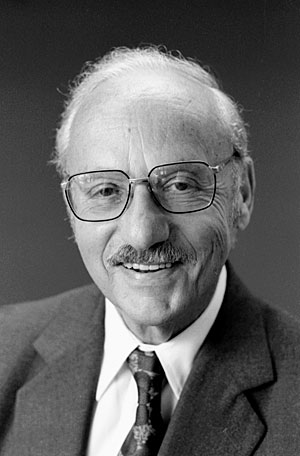
\includegraphics[width=300pt, height=455pt]{Dantzig}
          
\caption*{\textbf{George B. Dantzig} \\ 
Geb. 1914 in Portland, Oregon \\ 
Gest. 2005 in Stanford, Kalifornien}
\end{figure}

%------------------------------------------------------------------------------%
% Skript zu:                                                                   %
% "Optimierung f�r Studierende der Informatik"                                 %
% ============================================                                 %
%                                                                              %
% Kapitel 02:                                                                  %
% "Wie das Simplexverfahren funktioniert"                                      %
%                                                                              %
% in LaTeX gesetzt von:                                                        %
% Steven K�hler                                                                %
%                                                                              %
% Version:                                                                     %
% 2017-01-31                                                                   %
%------------------------------------------------------------------------------%


\chapter{Wie das Simplexverfahren funktioniert}\label{chapter:2}
\index{Simplexverfahren}\index{Verfahren!Simplex-}


%------------------------------------------------------------------------------%
% Abschnitt:                                                                   %
% "Die Axiome der reellen Zahlen"                                              %
%------------------------------------------------------------------------------%


Wir besprechen anhand des folgenden Beispiels, wie das Simplexverfahren verwendet wird, um LP-Probleme zu l�sen, die \textit{in Standardform}\index{Standardform} vorliegen:
\begin{align}
\begin{alignedat}{5}
\label{eq:2:1}
& \text{maximiere } & 5x_1 &\ + &\ 4x_2 &\ + &\ 3x_3 & & \\
& \rlap{unter den Nebenbedingungen} & & & & & & & \\
&& 2x_1 &\ + &\ 3x_2 &\ + &\  x_3 &\ \leq &\  5\ \\
&& 4x_1 &\ + &\  x_2 &\ + &\ 2x_3 &\ \leq &\ 11\ \\
&& 3x_1 &\ + &\ 4x_2 &\ + &\ 2x_3 &\ \leq &\  8\ \\
&& & & & & \llap{$x_1, x_2, x_3$} &\ \geq &\  0.
\end{alignedat}
\end{align}

Wir f�hren sogenannte \textit{Schlupfvariablen}\index{Schlupfvariable}\index{Variable!Schlupf-} (engl. \textit{slack variables}\index{slack variable}\index{Variable!slack}) ein. Worum es dabei geht, erkl�ren wir anhand der ersten Nebenbedingung:
\begin{equation}
\label{eq:2:2}
2x_1 + 3x_2 + x_3 \leq 5.
\end{equation}

Ist $x_1,x_2,x_3$ eine zul�ssige L�sung des LP-Problems (\ref{eq:2:1}), so erf�llen die Zahlen $x_1, x_2, x_3$ insbesondere die Ungleichung (\ref{eq:2:2}), wobei es m�glich ist, dass $2x_1+3x_2+x_3 < 5$ gilt, aber es k�nnte auch $2x_1+3x_2+x_3 = 5$ gelten. Die Differenz der rechten und der linken Seite von (\ref{eq:2:2}) bezeichnet man als \textit{Schlupf} (engl. \textit{slack}). Der Schlupf gibt also an, um wie viel die rechte Seite die linke Seite �bertrifft. Die Differenz zwischen der rechten und der linken Seite von (\ref{eq:2:2}) wollen wir $x_4$ nennen; wir \textit{definieren} also:
\[
x_4 = 5 - 2x_1 - 3x_2 - x_3.
\]

Mit dieser neuen Bezeichnung k�nnen wir die Ungleichung (\ref{eq:2:2}) kurz und knapp wie folgt ausdr�cken:
\[
x_4 \geq 0.
\]

In �hnlicher Weise definieren wir:
\begin{align*}
\begin{alignedat}{5}
x_5 &\ = &\ 11 &\ - &\ 4x_1 &\ - &\  x_2 &\ - &\ 2x_3\ \\
x_6 &\ = &\  8 &\ - &\ 3x_1 &\ - &\ 4x_2 &\ - &\ 2x_3.
\end{alignedat}
\end{align*}

Die neuen Variablen $x_4, x_5, x_6$ werden \textit{Schlupfvariablen} (bzw. \textit{slack variables}) genannt.

Dar�ber hinaus ist es �blich, noch eine weitere Variable einzuf�hren, die man mit $z$ bezeichnet und die den Wert der Zielfunktion angibt; in unserem Beispiel:
\[
z = 5x_1 + 4x_2 + 3x_3.
\]

Unsere �berlegungen lassen sich wie folgt zusammenfassen: Zu jeder Wahl der Zahlen $x_1,x_2,x_3$ definieren wir die Zahlen $x_4,x_5,x_6$ und $z$, indem wir festlegen:
\begin{align}
\begin{alignedat}{5}
\label{eq:2:3}
x_4 &\ = &\  5 &\ - &\ 2x_1 &\ - &\ 3x_2 &\ - &\  x_3\ \\
x_5 &\ = &\ 11 &\ - &\ 4x_1 &\ - &\  x_2 &\ - &\ 2x_3\ \\
x_6 &\ = &\  8 &\ - &\ 3x_1 &\ - &\ 4x_2 &\ - &\ 2x_3\ \\
z   &\ = &     &    &\ 5x_1 &\ + &\ 4x_2 &\ + &\ 3x_3.
\end{alignedat}
\end{align}

\textit{Unter Verwendung der Bezeichnungen $x_4,x_5,x_6$ und $z$ aus (\ref{eq:2:3}) k�nnen wir unser LP-Problem (\ref{eq:2:1}) auch wie folgt formulieren}:
\begin{align}
\begin{alignedat}{3}
\label{eq:2:4}
& \text{maximiere $z$} & & & \\
& \rlap{unter den Nebenbedingungen} & & &\\
&& x_1,x_2,x_3,x_4,x_5,x_6 &\ \geq &\ 0.
\end{alignedat}
\end{align}

Wir betonen noch einmal: Bei (\ref{eq:2:4}) handelt es sich nur um eine \textit{Umformulierung} von (\ref{eq:2:1}), wobei die Bezeichnungen $x_4$, $x_5$, $x_6$ und $z$ aus (\ref{eq:2:3}) verwendet werden. Es gilt:
\begin{enumerate}[(i)]
\item Jede zul�ssige L�sung $x_1,x_2,x_3$ von (\ref{eq:2:1}) kann auf eindeutige Art zu einer zul�ssigen L�sung von (\ref{eq:2:4}) erweitert werden, indem man $x_1$, $x_2$ und $x_3$ in (\ref{eq:2:3}) einsetzt.
\item Ist umgekehrt $x_1,x_2,x_3,x_4,x_5,x_6$ eine zul�ssige L�sung von (\ref{eq:2:4}), wobei $x_4$, $x_5$ und $x_6$ die in (\ref{eq:2:3}) angegebene Bedeutung haben, so kann man auf eine sehr einfache Art eine zul�ssige L�sung $x_1,x_2,x_3$ von (\ref{eq:2:1}) erhalten: Man braucht die Schlupfvariablen $x_4,x_5,x_6$ nur wegzulassen.
\end{enumerate}

\textit{Aufgrund von (i) und (ii) entsprechen sich die zul�ssigen L�sungen von (\ref{eq:2:1}) und (\ref{eq:2:4}) also umkehrbar eindeutig, wobei auch jeder optimalen L�sung von (\ref{eq:2:1}) eine optimale L�sung von (\ref{eq:2:4}) entspricht; und umgekehrt}. Man beachte, dass die Zielfunktion in beiden F�llen dieselbe ist.

Wir f�hren nun vor, wie man mithilfe des Simplexverfahrens eine optimale L�sung von (\ref{eq:2:1}) bzw. (\ref{eq:2:4}) findet. Die \textbf{Grundidee} ist einfach: Man versucht zul�ssige L�sungen schrittweise zu verbessern, wobei man anstrebt, nach endlich vielen Schritten bei einer optimalen L�sung anzukommen.

\textit{Mit anderen Worten}: Wenn wir eine zul�ssige L�sung $x_1,\ldots,x_6$ von (\ref{eq:2:4}) haben, so versuchen wir eine zul�ssige L�sung $x_1',\ldots,x_6'$ von (\ref{eq:2:4}) zu finden, f�r die gilt:
\[
5 x_1' + 4x_2' + 3 x_3' > 5x_1 + 4x_2 + 3x_3.
\]

Damit dieser Prozess in Gang kommt, braucht man nat�rlich eine zul�ssige \textbf{Startl�sung}\index{Startl�sung}\index{L�sung!Start-}. \textit{In unserem Beispiel ist es leicht, eine solche zu finden}: Wir w�hlen $x_1=x_2=x_3=0$.

Mithilfe von (\ref{eq:2:3}) erh�lt man dann dazugeh�rige Werte f�r $x_4$, $x_5$ und $x_6$:
\[
x_4 = 5, \qquad x_5 = 11, \qquad x_6 = 8.
\]

\textit{Unsere Startl�sung lautet also}:
\begin{equation}
\label{eq:2:5}
x_1=0, \qquad x_2=0, \qquad x_3=0, \qquad x_4 = 5, \qquad x_5 = 11, \qquad x_6 = 8.
\end{equation}

Hierbei handelt es sich in der Tat um eine zul�ssige L�sung von (\ref{eq:2:4}), da $x_1, \ldots, x_6$ so gew�hlt wurden, dass (\ref{eq:2:3}) gilt, und da au�erdem die Bedingungen $x_1,\ldots, x_6 \geq 0$ erf�llt sind.

Den zu dieser L�sung dazugeh�rigen \textit{Zielfunktionswert} $z$ erhalten wir ebenso, wie wir $x_4,x_5,x_6$ erhalten haben: Wir setzen in (\ref{eq:2:3}) f�r $x_1,x_2,x_3$ den Wert $0$ sein. Man erh�lt
\[
z=0.
\]

\textit{Dies gilt es nun zu verbessern, indem wir eine zul�ssige L�sung mit einem h�heren Zielfunktionswert $z$ finden}. \textbf{Das ist nicht schwer}: Lassen wir beispielsweise die Werte f�r $x_2$ und $x_3$ unver�ndert bei $x_2=x_3=0$ und vergr��ern $x_1$, so erhalten wir
\[
z = 5x_1 > 0.
\]
Beispielsweise k�nnten wir $x_2=x_3=0$ und $x_1=1$ w�hlen und erhielten die zul�ssige L�sung
\[
x_1=1, \qquad x_2=0, \qquad x_3=0, \qquad x_4=3, \qquad x_5=7, \qquad x_6=5 \quad \text{mit} \quad z=5.
\]

W�hlen wir $x_1=2$ und nach wie vor $x_2=x_3=0$, so erhalten wir einen noch besseren Zielfunktionswert: $z=10$. Au�erdem gilt $x_4=1$, $x_5=3$, $x_6=2$.

Versuchen wir dasselbe mit $x_1=3$ und $x_2=x_3=0$, so erhalten wir $z=15$, was ein noch besserer Zielfunktionswert w�re. Aber gleichzeitig erhalten wir auch $x_4 = -1$. \textit{Das bedeutet, dass wir den Bereich der zul�ssigen L�sungen verlassen haben}: Es muss ja immer $x_4 \geq 0$, $x_5 \geq 0$ und $x_6 \geq 0$ gelten. \textit{Wir haben $x_1$ also zu stark erh�ht}.

\textit{Frage}: Um wie viel k�nnen wir $x_1$ maximal erh�hen (unter Beibehaltung von $x_2=x_3=0$), ohne dass einer der Werte $x_4, x_5, x_6$ negativ wird?

\textit{Die Antwort auf diese Frage l�sst sich leicht an den ersten drei Zeilen von (\ref{eq:2:3}) ablesen}: Da $x_2=x_3=0$ gelten soll, haben wir
\begin{align*}
\begin{alignedat}{3}
x_4 &\ = &\  5 &\ - &\ 2x_1\ \\
x_5 &\ = &\ 11 &\ - &\ 4x_1\ \\
x_6 &\ = &\  8 &\ - &\ 3x_1.
\end{alignedat}
\end{align*}

Die Bedingung $x_4 \geq 0$ ist also gleichbedeutend mit $5 - 2x_1 \geq 0$, d.h., als Bedingung f�r $x_1$ erhalten wir $x_1 \leq \frac{5}{2}$. Entsprechend erh�lt man aus $x_5 \geq 0$ die Bedingung $x_1 \leq \frac{11}{4}$ und $x_6 \geq 0$ f�hrt zu $x_1 \leq \frac{8}{3}$. Die erste Bedingung schr�nkt $x_1$ am st�rksten ein; wir w�hlen also $x_1 = \frac{5}{2}$ und erhalten somit die zul�ssige L�sung
\begin{equation}
\label{eq:2:6}
x_1=\frac{5}{2}, \qquad x_2=0, \qquad x_3=0, \qquad x_4=0, \qquad  x_5=1, \qquad x_6=\frac{1}{2}.
\end{equation}

Als verbesserten Zielfunktionswert erhalten wir $z = \frac{25}{2}$.

\textit{Wir fassen das bisher Erreichte zusammen}: \textit{Unsere Startl�sung lautete}
\[
x_1=0, \qquad x_2=0, \qquad x_3=0, \qquad x_4=5, \qquad x_5=11, \qquad x_6=8 \quad \text{mit} \quad z=0,
\]

\textit{und in der 1. Iteration haben wir die verbesserte zul�ssige L�sung (\ref{eq:2:6}) mit $z = \frac{25}{2}$} erhalten.

Dies gilt es nun weiter zu verbessern. Die entscheidende Rolle in der 1. Iteration spielte das Gleichungssystem (\ref{eq:2:3}): \textit{Dort wurden die vier Variablen $x_4,x_5,x_6$ und $z$ durch die drei �brigen Variablen (n�mlich durch $x_1,x_2,x_3$) dargestellt und diese drei Variablen besa�en alle den Wert Null in unserer Startl�sung}.

Diesen Zustand wollen wir nun (bezogen auf die verbesserte L�sung (\ref{eq:2:6})) wiederherstellen. In (\ref{eq:2:6}) sind $x_2, x_3$ und $x_4$ diejenigen Variablen, die den Wert Null annehmen. Diese Variablen sollen nun die Rolle spielen, die zuvor von $x_1$, $x_2$ und $x_3$ gespielt wurde. Hierzu formen wir (\ref{eq:2:3}) so um, dass auf der linken Seite nun $x_1$, $x_5$, $x_6$ und $z$ stehen, w�hrend rechts nur noch die Variablen $x_2$, $x_3$ und $x_4$ auftauchen.

Anders gesagt: \textit{$x_1$ und $x_4$ sollen ihre Rollen tauschen; $x_1$ soll von rechts nach links wandern; $x_4$ umgekehrt von links nach rechts}.

Hierzu formen wir zun�chst diejenige Zeile von (\ref{eq:2:3}) um, in der $x_4$ auf der linken Seite steht. In (\ref{eq:2:3}) ist das die erste Zeile; wir erhalten
\begin{equation}
\label{eq:2:7}
x_1 = \frac{5}{2} - \frac{3}{2}x_2 - \frac{1}{2}x_3 - \frac{1}{2}x_4.
\end{equation}

Einsetzen von (\ref{eq:2:7}) in die �brigen Zeilen von (\ref{eq:2:3}) ergibt:
\begin{align*}
x_5 &= 11 - 4 \cdot \left( \frac{5}{2} - \frac{3}{2}x_2 - \frac{1}{2}x_3 - \frac{1}{2}x_4 \right) - x_2 - 2x_3 \\
    &= 1 + 5x_2 + 2x_4 \\
x_6 &= 8 - 3 \cdot \left( \frac{5}{2} - \frac{3}{2}x_2 - \frac{1}{2}x_3 - \frac{1}{2}x_4 \right) -4x_2 - 2x_3 \\
    &= \frac{1}{2} + \frac{1}{2}x_2 - \frac{1}{2}x_3 + \frac{3}{2}x_4 \\
z   &= 5 \cdot \left( \frac{5}{2} - \frac{3}{2}x_2 - \frac{1}{2}x_3 - \frac{1}{2}x_4 \right) + 4x_2 + 3x_3 \\
    &= \frac{25}{2} - \frac{7}{2}x_2 + \frac{1}{2}x_3 - \frac{5}{2}x_4.
\end{align*}

Also lautet unser neues, durch Umformung von (\ref{eq:2:3}) entstandenes Gleichungssystem:
\begin{align}
\begin{alignedat}{5}
\label{eq:2:8}
x_1 &\ = &\  \frac{5}{2} &\ - &\ \frac{3}{2}x_2 &\ - &\ \frac{1}{2}x_3 &\ - &\ \frac{1}{2}x_4\ \\
x_5 &\ = &\            1 &\ + &\           5x_2 &    &                 &\ + &\           2x_4\ \\
x_6 &\ = &\  \frac{1}{2} &\ + &\ \frac{1}{2}x_2 &\ - &\ \frac{1}{2}x_3 &\ + &\ \frac{3}{2}x_4\ \\
z   &\ = &\ \frac{25}{2} &\ - &\ \frac{7}{2}x_2 &\ + &\ \frac{1}{2}x_3 &\ - &\ \frac{5}{2}x_4.
\end{alignedat}
\end{align}

Analog zur 1. Iteration\index{Iteration} versuchen wir nun, den aktuellen Wert von $z$ zu vergr��ern, indem wir den Wert einer der drei Variablen auf der rechten Seite von (\ref{eq:2:8}) anheben, w�hrend wir gleichzeitig die beiden anderen Variablen der rechten Seite bei Null lassen. \textit{Wir haben drei M�glichkeiten zur Auswahl}:
\begin{enumerate}[(i)]
\item $x_2$ wird angehoben, $x_3=x_4=0$;
\item $x_3$ wird angehoben, $x_2=x_4=0$;
\item $x_4$ wird angehoben, $x_2=x_3=0$.
\end{enumerate}

Die \enquote{M�glichkeiten} (i) und (iii) scheiden sofort aus: Sie f�hren zu einer Verkleinerung von $z$ -- sehr entgegen unserer Absichten.

\text{Es bleibt nur eine Wahl}: Wir setzen $x_2=x_4=0$ und versuchen durch Anheben von $x_3$ zu einem m�glichst gro�en Zuwachs von $z$ zu gelangen, wobei wir allerdings darauf achten m�ssen, dass weiterhin $x_1 \geq 0$, $x_5 \geq 0$ und $x_6 \geq 0$ gilt.

\textit{Wie stark k�nnen wir $x_3$ anheben}? Die Antwort k�nnen wir direkt an unserem Gleichungssystem (\ref{eq:2:8}) ablesen: Wegen $x_2=x_4=0$ ist die Bedingung $x_1 \geq 0$ �quivalent zu $\frac{5}{2} - \frac{1}{2}x_3 \geq 0$, woraus man $x_3 \leq 5$ erh�lt. Aus $x_6 \geq 0$ erh�lt man auf �hnliche Art $x_3 \leq 1$, w�hrend die Bedingung $x_5 \geq 0$ die Wahl von $x_3$ nicht beschr�nkt. \textbf{Also}: \textit{$x_3=1$ ist das Beste, was wir erreichen k�nnen, und unsere neue L�sung ist dementsprechend}:
\begin{equation}
\label{eq:2:9}
x_1=2, \qquad x_2=0, \qquad x_3=1, \qquad x_4=0, \qquad x_5=1, \qquad x_6=0.
\end{equation}

Wir wissen bereits: \textit{Damit das Verfahren weitergeht, brauchen wir nicht nur eine verbesserte L�sung, sondern auch eine neue Darstellung unseres Gleichungssystems (\ref{eq:2:8}), die zu (\ref{eq:2:9}) passt}. In (\ref{eq:2:9}) gibt es drei Variablen, die den Wert Null annehmen: $x_2=x_4=x_6=0$. Diese drei Variablen sollen nun auf der rechten Seite stehen, die �brigen Variablen ($x_1,x_3,x_5$ sowie $z$) sollen links auftauchen: \textit{�hnlich wie in der ersten Iteration ist also ein \textbf{Austausch}\index{Austausch} vorzunehmen; diesmal haben $x_3$ und $x_6$ die Seiten zu wechseln}. Dementsprechend stellen wir die dritte Gleichung von (\ref{eq:2:8}) um und erhalten
\[
x_3 = 1 + x_2 + 3x_4 - 2x_6.
\]

Setzt man dies f�r $x_3$ in die �brigen Gleichungen von (\ref{eq:2:8}) ein, so erh�lt man
\begin{align}
\begin{alignedat}{5}
\label{eq:2:10}
x_3 &\ = &\  1 &\ + &\  x_2 &\ + &\ 3x_4 &\ - &\ 2x_6\ \\
x_1 &\ = &\  2 &\ - &\ 2x_2 &\ - &\ 2x_4 &\ + &\  x_6\ \\
x_5 &\ = &\  1 &\ + &\ 5x_2 &\ + &\ 2x_4 &    &        \\
z   &\ = &\ 13 &\ - &\ 3x_2 &\ - &\  x_4 &\ - &\  x_6.
\end{alignedat}
\end{align}

Einsetzen von $x_2=x_4=x_6=0$ in die letzten Zeile von (\ref{eq:2:10}) ergibt $z=13$.

\textit{W�hrend sich in der ersten Iteration eine Steigerung des Zielfunktionswerts von $z=0$ zu $z=12.5$ ergeben hat, hat die zweite Iteration nur zu einem bescheidenen Zuwachs gef�hrt: $z=13$}.

Nun sollen Sie sich aber auch daran gew�hnen, dass das Lesen von englischen Lehrb�chern in der Regel sehr einfach ist. Darum gibt es den Rest auf Englisch (Originaltext von Va\v{s}ek Chv�tal).

\medskip

Now it's time for the third iteration. First of all, from the right-hand side of (\ref{eq:2:10}) we have to choose a variable whose increase brings about an increase of the objective function. However, there is no such variable: indeed, if we increase any of the right-hand side variables $x_2$, $x_4$, $x_6$, we will make the value of $z$ \textit{decrease}. Thus, it seems that we have come to a standstill. In fact, the very presence of this standstill indicates that we are done; we have solved our problem; the solution described by the last table is optimal. Why? The answer lies hidden in the last row of (\ref{eq:2:10}):
\begin{equation}
\label{eq:2:11}
z = 13 - 3x_2 - x_4 - x_6.
\end{equation}

Our last solution (\ref{eq:2:9}) yields $z=13$; proving that this solution is optimal amounts to proving that every feasible solution satisfies the inequality $z \leq 13$. Since every feasible solution $x_1,\ldots,x_6$ satisfies, among other relations, the inequalities $x_2 \geq 0$, $x_4 \geq 0$, and $x_6 \geq 0$, the desired inequality $z \leq 13$ follows directly from (\ref{eq:2:11}).

\medskip

Auf Deutsch (etwas frei �bersetzt):

\textit{Bei der dritten Iteration stecken wir fest}. Was nun zun�chst wie eine Schwierigkeit aussieht, entpuppt sich als Erfolg: \textit{Die L�sung (\ref{eq:2:9}) ist optimal, der Zielfunktionswert $z=13$ ist bestm�glich. Weshalb ist das so?} \textbf{Die Antwort findet sich in der letzten Zeile von (\ref{eq:2:10})}:
\begin{equation}
\tag{\ref*{eq:2:11}}
z = 13 - 3x_2 - x_4 - x_6.
\end{equation}

Unsere letzte L�sung (\ref{eq:2:9}) hat zu $z=13$ gef�hrt. \textit{Wir wollen uns davon �berzeugen, dass f�r jede zul�ssige L�sung $z \leq 13$ gilt}. Aufgrund von (\ref{eq:2:11}) ist dies aber klar: Ist $x_1,x_2,x_3,x_4,x_5,x_6$ eine beliebige zul�ssige L�sung, so gilt insbesondere $x_2 \geq 0$, $x_4 \geq 0$ und $x_6 \geq 0$, woraus sich (aufgrund von (\ref{eq:2:11})) $z \leq 13$ ergibt.

\bigskip

Nachdem wir das Simplexverfahren anhand eines Beispiels studiert haben, schauen wir uns nun den allgemeinen Fall an. Gegeben sei ein LP-Problem in Standardform.

\begin{SKBox}
\textbf{LP-Problem in Standardform}.
\begin{align}
\begin{alignedat}{3}
\label{eq:2:12}
& \text{maximiere } & \sum\limits_{j=1}^{n}{c_jx_j} & & \\
& \rlap{unter den Nebenbedingungen} & & & \\
&& \sum\limits_{j=1}^{n}{a_{ij}x_j} &\ \leq &\ b_i \qquad (i=1,\ldots, m)\ \\
&& x_j &\ \geq &\ 0 \qquad (j=1,\ldots,n).
\end{alignedat}
\end{align}
\end{SKBox}

Wollen wir das LP-Problem (\ref{eq:2:12}) mit dem Simplexverfahren l�sen, so f�hren wir zun�chst \textit{Schlupfvariablen}\index{Schlupfvariable}\index{Variable!Schlupf-} $x_{n+1}, \ldots, x_{n+m}$ sowie eine Variable $z$ ein, die den Wert der \textit{Zielfunktion} angibt. \textit{Mit anderen Worten: Wir definieren}
\begin{align}
\begin{alignedat}{3}
\label{eq:2:13}
x_{n+i} &\ = &\ b_i &\ - &\ \sum\limits_{j=1}^{n}{a_{ij}x_j} & \qquad (i = 1,\ldots, m) \\
      z &\ = &\     &    &\ \sum\limits_{j=1}^{n}{c_jx_j}. &
\end{alignedat}
\end{align}

Unter Verwendung der Bezeichnungen aus (\ref{eq:2:13}) kann man das LP-Problem (\ref{eq:2:12}) auch wie folgt schreiben:
\begin{align}
\label{eq:2:12'}
\tag{\ref*{eq:2:12}'}
\begin{alignedat}{3}
& \text{maximiere $z$} & & & \\
& \rlap{unter den Nebenbedingungen} & & & \\
&& x_1,\ldots,x_{n+m} &\ \geq &\ 0.
\end{alignedat}
\end{align}

Die folgende h�ufig verwendete M�glichkeit, das LP-Problem (\ref{eq:2:12}) zu formulieren, ergibt sich direkt aus der Definition der Schlupfvariablen:

\begin{SKBox}
\begin{align}
\label{eq:2:12''}
\tag{\ref*{eq:2:12}''}
\begin{alignedat}{4}
& \text{maximiere } & \sum\limits_{j=1}^{n}{c_jx_j} & & & & \\
& \rlap{unter den Nebenbedingungen} & & & & & \\
&& \sum\limits_{j=1}^{n}{a_{ij}x_j} &\ + &\ x_{n+i} &\ = &\ b_i & \qquad (i=1,\ldots,m)\ \\
&& & & x_j &\ \geq &\ 0 & \qquad (j=1,\ldots,n+m).
\end{alignedat}
\end{align}
\end{SKBox}

Im Verlauf des Simplexverfahrens ersetzt man in jeder Iteration eine zul�ssige L�sung $x_1, \ldots, x_{n+m}$ von (\ref{eq:2:12''}) durch eine zul�ssige L�sung $\overline{x}_1, \ldots, \overline{x}_{n+m}$; dabei strebt man an, dass die neue L�sung besser als die alte ist, d.h., man m�chte erhalten, dass
\[
\sum\limits_{j=1}^{n}{c_j\overline{x}_j} > \sum\limits_{j=1}^{n}{c_jx_j}
\]

gilt. In unserem obigen Beispiel wurde dies in jeder Iteration erreicht; \textit{wir werden jedoch (sp�ter) noch sehen, dass es auch n�tig sein kann, Iterationen zuzulassen, in denen $\sum\limits_{j=1}^{n}{c_j\overline{x}_j} = \sum\limits_{j=1}^{n}{c_jx_j}$ gilt}.

In unserem obigen Beispiel haben wir gesehen, dass in jeder Iteration nicht nur eine zul�ssige L�sung $x_1, \ldots, x_{n+m}$ ermittelt wird, sondern dass in jeder Iteration auch ein lineares Gleichungssystem mit $m+1$ Gleichungen vorkommt. In unserem Beispiel waren dies die Gleichungssysteme (\ref{eq:2:3}), (\ref{eq:2:8}) und (\ref{eq:2:10}). Die Variablen dieser Gleichungssysteme waren $x_1,\ldots,x_6$ und $z$, \textit{und diese Gleichungssysteme hatten eine besondere Form}: Links traten immer drei der Variablen $x_1,\ldots,x_6$ auf sowie (in der letzten Zeile) $z$, w�hrend rechts immer nur die drei �brigen der Variablen $x_1, \ldots, x_6$ vorkamen.

Au�erdem sind (wie man sich unschwer �berlegt) die drei Gleichungssysteme (\ref{eq:2:3}), (\ref{eq:2:8}) und (\ref{eq:2:10}) �quivalent in dem Sinne, dass sie \textit{dieselbe L�sungsmenge} besitzen. Anders gesagt: F�r jede Wahl der Zahlen $x_1, \ldots, x_6$ und $z$ sind die folgenden drei Aussagen �quivalent:
\begin{itemize}
\item $x_1,\ldots,x_6$ und $z$ bilden eine L�sung von (\ref{eq:2:3});
\item $x_1,\ldots,x_6$ und $z$ bilden eine L�sung von (\ref{eq:2:8});
\item $x_1,\ldots,x_6$ und $z$ bilden eine L�sung von (\ref{eq:2:10}).
\end{itemize}

F�r Gleichungssysteme wie (\ref{eq:2:3}), (\ref{eq:2:8}) und (\ref{eq:2:10}) gibt es \textbf{unterschiedliche Bezeichnungen}:
\begin{itemize}
\item Chv�tal benutzt beispielsweise die Bezeichnung \textit{dictionary};
\item im Buch von Cormen et al wird die Bezeichnung \textit{Schlupfform}\index{Schlupfform} benutzt;
\item im Buch von Matou\v{s}ek und G�rtner werden derartige Gleichungssysteme \textit{Tableaus} genannt.
\end{itemize}

Wir schlie�en uns der Sprechweise von Matou\v{s}ek und G�rtner an und verwenden ebenfalls den Begriff \textit{Tableau} als unsere Bezeichnung f�r Gleichungssysteme wie (\ref{eq:2:3}), (\ref{eq:2:8}) und (\ref{eq:2:10}). Wenn wir von einem Tableau sprechen, so ist damit also kein \enquote{Zahlenschema} oder \enquote{Koeffizientenschema} gemeint, sondern ein lineares Gleichungssystem einer bestimmten Art. Diejenigen Variablen $x_j$, die in einem Tableau auf der linken Seite stehen, nennt man \textit{Basisvariablen}, die �brigen Variablen $x_j$, also diejenigen, die auf der rechten Seite stehen, nennt man \textit{Nichtbasisvariablen}. Die Menge der Basisvariablen nennt man eine \textit{Basis}\index{Basis}; wir bezeichnen die Menge der zu den Basisvariablen $x_j$ geh�renden Indizes $j$ mit $B$; die Menge der Indizes $j$, die bei den Nichtbasisvariablen vorkommen, bezeichnen wir mit $N$.

Im Verlauf des Simplexalgorithmus �ndern sich $B$ und $N$; wir erl�utern dies anhand unseres Beispiels.

F�r das Tableau (\ref{eq:2:3}) gilt $B = \bigl\{ 4,5,6 \bigr\}$ und $N = \bigl\{ 1,2,3 \bigr\}$. Beim �bergang von (\ref{eq:2:3}) zum Tableau (\ref{eq:2:8}) verl�sst $x_4$ die Basis und $x_1$ wird neu in die Basis aufgenommen; f�r das Tableau (\ref{eq:2:8}) gilt also $B = \bigl\{ 1,5,6 \bigr\}$ und $N = \bigl\{ 2,3,4 \bigr\}$.

Einen �bergang von einem Tableau zum n�chsten (wie von (\ref{eq:2:3}) zu (\ref{eq:2:8})) nennt man \textit{Pivotschritt}\index{Pivotschritt}, \textit{Basisaustauschschritt}\index{Basisaustauschschritt} oder \textit{Basistausch}\index{Basistausch}; diejenige Variable, die neu in die Basis aufgenommen wird, hei�t \textit{Eingangsvariable}\index{Eingangsvariable}\index{Variable!Eingangs-}; die Variable, die die Basis verl�sst, hei�t \textit{Ausgangsvariable}\index{Ausgangsvariable}\index{Variable!Ausgangs-}. Diejenige Zeile, in der vor dem Basistausch links die Ausgangsvariable steht, hei�t \textit{Pivotzeile}\index{Pivotzeile}. Diejenige Spalte, in der vor dem Basistausch die Eingangsvariable steht, hei�t \textit{Pivotspalte}\index{Pivotspalte}.

Beim �bergang von (\ref{eq:2:8}) zu (\ref{eq:2:10}) ist $x_3$ die Eingangsvariable und $x_6$ ist die Ausgangsvariable. Die Zeile von (\ref{eq:2:8}), in der $x_6$ steht, ist die Pivotzeile dieses Basistauschs; die Spalte von (\ref{eq:2:8}), in der $x_3$ steht, ist die Pivotspalte.

Wir kehren zur�ck zum allgemeinen Fall (\ref{eq:2:12}). Unter einem zu (\ref{eq:2:12}) geh�rigen \textit{Tableau}\index{Tableau} (engl. Bezeichnung im Buch von Chv�tal: \textit{dictionary}\index{dictionary}) \label{page:2:1} verstehen wir ein System von $m+1$ linearen Gleichungen mit den Variablen $x_1,\ldots,x_{n+m}$ und $z$ sowie mit den folgenden Eigenschaften:
\begin{enumerate}[(i)]
\item Jede L�sung dieses Gleichungssystems ist eine L�sung von (\ref{eq:2:13}); und umgekehrt.
\item Die Gleichungen sind nach $m$ der Variablen $x_1,\ldots,x_{n+m}$ (genannt \textit{Basisvariablen}\index{Basisvariable}\index{Variable!Basis-}) und nach $z$ aufgel�st; die �brigen $n$ Variablen hei�en \textit{Nichtbasisvariablen}\index{Nichtbasisvariable}\index{Basisvariable!Nicht-}\index{Variable!Nichtbasis-}. Jede der Basisvariablen $x_j$ sowie $z$ ist im Gleichungssystem als Summe aus einer Konstanten und einer Linearkombination der Nichtbasisvariablen dargestellt.
\end{enumerate}

Etwas vereinfacht kann man (ii) auch so aussprechen: \textit{Jede Basisvariable $x_j$ sowie $z$ wird durch die Nichtbasisvariablen ausgedr�ckt}.

Die Eigenschaften (i) und (ii) definieren, was man unter einem \textit{Tableau} (engl. \textit{dictionary}) versteht. Die Tableaus (\ref{eq:2:3}), (\ref{eq:2:8}) und (\ref{eq:2:10}) besa�en dar�ber hinaus noch die folgende Eigenschaft:
\begin{enumerate}[(i)]
\addtocounter{enumi}{2}
\item  Werden auf der rechten Seite alle Variablen gleich Null gesetzt, so erh�lt man eine zul�ssige L�sung. (Mit anderen Worten: Setzt man alle Nichtbasisvariablen gleich Null, so wird keine der Basisvariablen negativ.)
\end{enumerate}

Tableaus mit dieser zus�tzlichen Eigenschaft werden \textit{zul�ssige Tableaus} (engl. \textit{feasible dictionaries}) genannt.
\index{zul�ssiges Tableau}\index{Tableau!zul�ssiges}\index{feasible dictionary}\index{dictionary!feasible}

\textit{Jedes zul�ssige Tableau beschreibt also eine zul�ssige L�sung von (\ref{eq:2:12}), die man erh�lt, wenn man alle Nichtbasisvariablen gleich Null setzt}. Aber nicht jede zul�ssige L�sung entsteht auf diese Art aus einem zul�ssigen Tableau; beispielsweise ist
\[
x_1=1,\quad x_2=0,\quad x_3=1,\quad x_4=2,\quad x_5=5,\quad x_6=3
\]
eine zul�ssige L�sung von (\ref{eq:2:1}), die jedoch nicht von einem zul�ssigen Tableau auf die beschriebene Weise abstammt.

Zul�ssige L�sungen, die durch ein Tableau beschrieben werden (d.h., die aus einem Tableau dadurch entstehen, dass man alle Nichtbasisvariablen auf Null setzt), hei�en \textit{zul�ssige Basisl�sungen} (engl. \textit{basic feasible solutions}).
\index{zul�ssige Basisl�sung}\index{Basisl�sung, zul�ssige}\index{L�sung!zul�ssige Basis-}
\index{basic feasible solution}\index{solution!basic feasible}

\textit{Eine auffallende Eigenschaft des Simplexalgorithmus ist, dass er nur mit zul�ssigen Basisl�sungen arbeitet und alle anderen zul�ssigen L�sungen ignoriert}.

Nun ist es Zeit f�r ein weiteres \textbf{Beispiel}, das aus Chv�tal: \textit{Linear Programming} entnommen wurde.

\medskip
\textbf{Second Example}

We shall complete our preview of the simplex method by applying it to another LP problem:

\footnotesize
\begin{align*}
\begin{alignedat}{5}
& \text{maximize } & 5x_1 &\ + &\ 5x_2 &\ + &\ 3x_3 & & \\
& \rlap{subject to} & & & & & & & \\
&&  x_1 &\ + &\ 3x_2 &\ + &\  x_3 &\ \leq &\ 3\ \\
&& -x_1 &\   &\      &\ + &\ 3x_3 &\ \leq &\ 2\ \\
&& 2x_1 &\ - &\  x_2 &\ + &\ 2x_3 &\ \leq &\ 4\ \\
&& 2x_1 &\ + &\ 3x_2 &\ - &\  x_3 &\ \leq &\ 2\ \\
&& & & & & \llap{$x_1, x_2, x_3$} &\ \geq &\ 0.
\end{alignedat}
\end{align*}

\small
In this case, the initial feasible dictionary reads
\begin{align}
\begin{alignedat}{5}
\label{eq:2:c1}
x_4 &\ = &\ 3 &\ - &\  x_1 &\ - &\ 3x_2 &\ - &\  x_3\ \\
x_5 &\ = &\ 2 &\ + &\  x_1 &\   &\      &\ - &\ 3x_3\ \\
x_6 &\ = &\ 4 &\ - &\ 2x_1 &\ + &\  x_2 &\ - &\ 2x_3\ \\
x_7 &\ = &\ 2 &\ - &\ 2x_1 &\ - &\ 3x_2 &\ + &\  x_3\ \\ \cline{1-9}
  z &\ = &\   &\   &\ 5x_1 &\ + &\ 5x_2 &\ + &\ 3x_3.
\end{alignedat}
\end{align}

(Even though the order of the equations in a dictionary is quite irrelevant, we shall make a habit of writing the formula for $z$ last and separating it from the rest of the table by a solid line. Of course, that does \textit{not} mean that the last equation is the sum of the previous ones.) This feasible dictionary describes the feasible solution
\[
x_1 = 0,\quad
x_2 = 0,\quad
x_3 = 0,\quad
x_4 = 3,\quad
x_5 = 2,\quad
x_6 = 4,\quad
x_7 = 2.
\]

However, there is no need to write this solution down, as we just did: the solution is implicit in the dictionary.

In the first iteration, we shall attempt to increase the value of $z$ by making one of the right-hand side variables positive. At this moment, any of the three variables $x_1$, $x_2$, $x_3$ would do. In small examples, it is common practice to choose the variable that, in the formula for $z$, has the largest coefficient: the increase in that variable will make $z$ increase at the fastest rate (but not necessarily to the highest level). In our case, this rule leaves us a choice between $x_1$ and $x_2$; choosing arbitrarily, we decide to make $x_1$ positive. As the value of $x_1$ increases, so does the value of $x_5$. However, the values of $x_4$, $x_6$, and $x_7$ decrease, and none of them is allowed to become negative. Of the three constraints $x_4 \geq 0$, $x_6 \geq 0$, $x_7 \geq 0$ that impose upper bounds on the increment of $x_1$ the last constraint $x_7 \geq 0$ is the most stringent: it implies $x_1 \leq 1$. In the improved feasible solution, we shall have $x_1=1$ and $x_7 = 0$. Without writing the new solution down, we shall now construct the new dictionary. All we need to know is that $x_1$ just made its way from the right-hand side to the left, whereas $x_7$ went in the opposite direction. From the fourth equation in (\ref{eq:2:c1}), we have
\begin{equation}
\label{eq:2:c2}
x_1 = 1 - \frac{3}{2}x_2 + \frac{1}{2}x_3 - \frac{1}{2}x_7.
\end{equation}


Substituting from (\ref{eq:2:c2}) into the remaining equations of (\ref{eq:2:c1}), we arrive at the desired dictionary

\begin{align}
\begin{alignedat}{5}
\label{eq:2:c3}
x_1 &\ = &\ 1 &\ - &\ \frac{3}{2}x_2 &\ + &\  \frac{1}{2}x_3 &\ - &\ \frac{1}{2}x_7\ \\[1mm]
x_4 &\ = &\ 2 &\ - &\ \frac{3}{2}x_2 &\ - &\  \frac{3}{2}x_3 &\ + &\ \frac{1}{2}x_7\ \\[1mm]
x_5 &\ = &\ 3 &\ - &\ \frac{3}{2}x_2 &\ - &\  \frac{5}{2}x_3 &\ - &\ \frac{1}{2}x_7\ \\[1mm]
x_6 &\ = &\ 2 &\ + &\           4x_2 &\ - &\            3x_3 &\ + &\            x_7\ \\[1mm] \cline{1-9}
  z &\ = &\ 5 &\ - &\ \frac{5}{2}x_2 &\ + &\ \frac{11}{2}x_3 &\ - &\ \frac{5}{2}x_7.
\end{alignedat}
\end{align}

The construction of (\ref{eq:2:c3}) completes the first iteration of the simplex method.

In our example, the variable to enter the basis during the second iteration is quite unequivocally $x_3$. This is the only nonbasic variable in (\ref{eq:2:c3}) whose coefficient in the last row is positive. Of the four basic variables, $x_6$ imposes the most stringent upper bound on the increase of $x_3$, and, therefore, has to leave the basis. Pivoting, we arrive at our third dictionary,
\begin{align}
\begin{alignedat}{5}
\label{eq:2:c4}
x_3 &\ = &\ \frac{ 2}{3} &\ + &\ \frac{ 4}{3}x_2 &\ + &\ \frac{1}{3}x_7 &\ - &\ \frac{ 1}{3}x_6\ \\[1mm]
x_1 &\ = &\ \frac{ 4}{3} &\ - &\ \frac{ 5}{6}x_2 &\ - &\ \frac{1}{3}x_7 &\ - &\ \frac{ 1}{6}x_6\ \\[1mm]
x_4 &\ = &\            1 &\ - &\ \frac{ 7}{2}x_2 &\   &\                &\ + &\ \frac{ 1}{2}x_6\ \\[1mm]
x_5 &\ = &\ \frac{ 4}{3} &\ - &\ \frac{29}{6}x_2 &\ - &\ \frac{4}{3}x_7 &\ + &\ \frac{ 5}{6}x_6\ \\[1mm] \cline{1-9}
  z &\ = &\ \frac{26}{3} &\ + &\ \frac{29}{6}x_2 &\ - &\ \frac{2}{3}x_7 &\ - &\ \frac{11}{6}x_6.
\end{alignedat}
\end{align}

In the third iteration, the entering variable is $x_2$ and the leaving variable is $x_5$. Pivoting yields the dictionary
\begin{align}
\begin{alignedat}{5}
\label{eq:2:c5}
x_2 &\ = &\ \frac{ 8}{29} &\ - &\ \frac{ 8}{29}x_7 &\ + &\ \frac{5}{29}x_6 &\ - &\ \frac{ 6}{29}x_5\ \\[1mm]
x_3 &\ = &\ \frac{30}{29} &\ - &\ \frac{ 1}{29}x_7 &\ - &\ \frac{3}{29}x_6 &\ - &\ \frac{ 8}{29}x_5\ \\[1mm]
x_1 &\ = &\ \frac{32}{29} &\ - &\ \frac{ 3}{29}x_7 &\ - &\ \frac{9}{29}x_6 &\ + &\ \frac{ 5}{29}x_5\ \\[1mm]
x_4 &\ = &\ \frac{ 1}{29} &\ + &\ \frac{28}{29}x_7 &\ - &\ \frac{3}{29}x_6 &\ + &\ \frac{21}{29}x_5\ \\[1mm] \cline{1-9}
  z &\ = &\            10 &\ - &\             2x_7 &\ - &\             x_6 &\ - &\              x_5.
\end{alignedat}
\end{align}

At this point, no nonbasic variable can enter the basis without making the value of $z$ decrease. Hence, the last dictionary describes an optimal solution of our example. That solution is
\[
x_1 = \frac{32}{29}, \quad
x_2 = \frac{8}{29}, \quad
x_3 = \frac{30}{29}
\]
and it yields $z = 10$.










Das \textit{Ergebnis einer Iteration}\index{Ergebnis einer Iteration}\index{Iteration!Ergebnis einer} ist immer ein \textit{neues Tableau}. \textit{Am Ende jeder Iteration wird dieses Ergebnis -- das neue Tableau also -- �bersichtlich hingeschrieben}, wobei einige \textit{Konventionen}\index{Konventionen beim Simplexverfahren}\index{Simplexverfahren!Konventionen beim} zu beachten sind, die wir im zweiten Beispiel kennengelernt haben\footnote{Diese Konventionen dienen der �bersichtlichkeit.}:

\begin{enumerate}
\item Die $z$-Zeile\index{$z$-Zeile} wird \textbf{unten} notiert und durch einen Strich abgetrennt.
\item Im neuen Tableau wird die Zeile mit der Eingangsvariablen immer \textbf{oben} hingeschrieben.
\item Die Variable, die neu auf der rechten Seite auftaucht -- die Ausgangsvariable -- schlie�t immer \textbf{rechts} an.
\item Au�erdem ist es f�r die �bersichtlichkeit wichtig, dass im Tableau gleiche Variablen immer \textbf{genau untereinander} geschrieben werden.
\end{enumerate}

Wir schreiben das erste Beispiel noch einmal �bersichtlich auf. Dieses Beispiel kann als \textit{Muster f�r das L�sen von �bungsaufgaben}\index{Muster f�r das L�sen von �bungsaufgaben}\index{�bungsaufgaben, Muster f�r das L�sen von} dienen.

\textbf{Aufgabe}: L�sen Sie das folgende LP-Problem mit dem Simplexverfahren:
\begin{align*}
\begin{alignedat}{5}
& \text{maximiere } & 5x_1 &\ + &\ 4x_2 &\ + &\ 3x_3 & & \\
& \rlap{unter den Nebenbedingungen} & & & & & & & \\
&& 2x_1 &\ + &\ 3x_2 &\ + &\  x_3 &\ \leq &\  5\ \\
&& 4x_1 &\ + &\  x_2 &\ + &\ 2x_3 &\ \leq &\ 11\ \\
&& 3x_1 &\ + &\ 4x_2 &\ + &\ 2x_3 &\ \leq &\  8\ \\
&& & & & & \llap{$x_1, x_2, x_3$} &\ \geq &\  0.
\end{alignedat}
\end{align*}

\textbf{L�sung}.

\underline{Starttableau}:
\begin{align*}
\begin{alignedat}{5}
x_4 &\ = &\  5 &\ - &\ 2x_1 &\ - &\ 3x_2 &\ - &\  x_3\ \\
x_5 &\ = &\ 11 &\ - &\ 4x_1 &\ - &\  x_2 &\ - &\ 2x_3\ \\
x_6 &\ = &\  8 &\ - &\ 3x_1 &\ - &\ 4x_2 &\ - &\ 2x_3\ \\ \cline{1-9}
  z &\ = &     &    &\ 5x_1 &\ + &\ 4x_2 &\ + &\ 3x_3. 
\end{alignedat}
\end{align*}

\underline{1. Iteration}:

Eingangsvariable: $x_1$ \\
Ausgangsvariable: $x_4$

Es folgt
\begin{align*}
x_1 &= \frac{5}{2} - \frac{3}{2}x_2 - \frac{1}{2}x_3 - \frac{1}{2}x_4\ \\[2mm]
x_5 &= 11 - 4 \cdot \left( \frac{5}{2} - \frac{3}{2}x_2 - \frac{1}{2}x_3 - \frac{1}{2}x_4 \right) - x_2 - 2x_3 \\[2mm]
    &= 1 + 5x_2 + 2x_4 \\[2mm]
x_6 &= 8 - 3 \cdot \left( \frac{5}{2} - \frac{3}{2}x_2 - \frac{1}{2}x_3 - \frac{1}{2}x_4 \right) -4x_2 - 2x_3 \\[2mm]
    &= \frac{1}{2} + \frac{1}{2}x_2 - \frac{1}{2}x_3 + \frac{3}{2}x_4 \\[2mm]
z   &= 5 \cdot \left( \frac{5}{2} - \frac{3}{2}x_2 - \frac{1}{2}x_3 - \frac{1}{2}x_4 \right) + 4x_2 + 3x_3 \\[2mm]
    &= \frac{25}{2} - \frac{7}{2}x_2 + \frac{1}{2}x_3 - \frac{5}{2}x_4.
\end{align*}

\underline{Ergebnis der 1. Iteration}:

\begin{align*}
\begin{alignedat}{5}
x_1 &\ = &\  \frac{5}{2} &\ - &\ \frac{3}{2}x_2 &\ - &\ \frac{1}{2}x_3 &\ - &\ \frac{1}{2}x_4\ \\[2mm]
x_5 &\ = &\            1 &\ + &\           5x_2 &    &                 &\ + &\           2x_4\ \\[2mm]
x_6 &\ = &\  \frac{1}{2} &\ + &\ \frac{1}{2}x_2 &\ - &\ \frac{1}{2}x_3 &\ + &\ \frac{3}{2}x_4\ \\[2mm] \cline{1-9}
z   &\ = &\ \frac{25}{2} &\ - &\ \frac{7}{2}x_2 &\ + &\ \frac{1}{2}x_3 &\ - &\ \frac{5}{2}x_4.
\end{alignedat}
\end{align*}

\underline{2. Iteration}:

Eingangsvariable: $x_3$ \\
Ausgangsvariable: $x_6$

Es folgt
\begin{align*}
x_3 &= 1 + x_2 + 3x_4 - 2x_6 \\[2mm]
x_1 &= \frac{5}{2} - \frac{3}{2}x_2 - \frac{1}{2} \Bigl( 1+x_2+3x_4-2x_6 \Bigr) - \frac{1}{2}x_4 \\[2mm]
    &= 2 - 2x_2 - 2x_4 + x_6\ \\[2mm]
z   &= \frac{25}{2} - \frac{7}{2}x_2 + \frac{1}{2} \Bigl( 1+x_2+3x_4-2x_6 \Bigr) - \frac{5}{2}x_4 \\[2mm]
    &= 13 - 3x_2 -  x_4 - x_6.
\end{align*}

\underline{Ergebnis der 2. Iteration}:

\begin{align*}
\begin{alignedat}{5}
x_3 &\ = &\  1 &\ + &\  x_2 &\ + &\ 3x_4 &\ - &\ 2x_6\ \\
x_1 &\ = &\  2 &\ - &\ 2x_2 &\ - &\ 2x_4 &\ + &\  x_6\ \\
x_5 &\ = &\  1 &\ + &\ 5x_2 &\ + &\ 2x_4 &    &        \\ \cline{1-9}
z   &\ = &\ 13 &\ - &\ 3x_2 &\ - &\  x_4 &\ - &\  x_6.
\end{alignedat}
\end{align*}

Dieses Tableau liefert die optimale L�sung $x_1=2$, $x_2=0$, $x_3=1$ mit $z=13$.

Anstelle von \enquote{Ergebnis der $k$-ten Iteration} kann man jedes Mal auch kurz und knapp \enquote{Neues Tableau} schreiben.

\textbf{Hinweis}: Das \textit{Ergebnis einer Iteration}\index{Ergebnis einer Iteration}\index{Iteration!Ergebnis einer} ist nat�rlich auch immer eine \textbf{neue zul�ssige Basisl�sung}\index{zul�ssige Basisl�sung}\index{Basisl�sung, zul�ssige}. Die neue zul�ssige Basisl�sung braucht am Ende einer Iteration aber nicht unbedingt hingeschrieben zu werden, da sie implizit im neuen Tableau enthalten und sehr leicht ablesbar ist.

Der Deutlichkeit halber geben wir f�r das erste Beispiel die Folge der zul�ssigen Basisl�sungen noch einmal explizit an.

\underline{Startl�sung (\enquote{zul�ssige Basisl�sung am Anfang})}:
\[
x_1=0, \qquad x_2=0, \qquad x_3=0, \qquad x_4=5, \qquad x_5=11, \qquad x_6=8 \quad \text{mit} \quad z=0.
\]

\underline{Zul�ssige Basisl�sung nach der 1. Iteration}:
\[
x_1=\frac{5}{2}, \qquad x_2=0, \qquad x_3=0, \qquad x_4=0, \qquad x_5=1, \qquad x_6=\frac{1}{2} \quad \text{mit} \quad z=12.5.
\]

\underline{Zul�ssige Basisl�sung nach der 2. Iteration}:
\[
x_1=2, \qquad x_2=0, \qquad x_3=1, \qquad x_4=0, \qquad x_5=1, \qquad x_6=0 \quad \text{mit} \quad z=13.
\]

Abschlie�end noch eine \textbf{Sprechweise}: Im LP-Problem (\ref{eq:2:12}) hatten wir es urspr�nglich mit den Variablen $x_1,\ldots,x_n$ zu tun. Anschlie�end kamen sofort weitere Variablen $x_{n+1}, \ldots, x_{n+m}$ hinzu, die wir \textit{Schlupfvariablen} genannt haben. Um uns besser ausdr�cken zu k�nnen, fehlt noch ein Name f�r die \enquote{urspr�nglichen Variablen} $x_1,\ldots,x_n$: Es ist �blich, diese Variablen als \textit{Problemvariablen}\index{Problemvariable}\index{Variable!Problem-} oder \textit{Entscheidungsvariablen}\index{Entscheidungsvariable}\index{Variable!Entscheidungs-} (engl. \textit{decision variables}\index{decision variable}\index{Variable!decision}) zu bezeichnen.

%------------------------------------------------------------------------------%
% Skript zu:                                                                   %
% "Optimierung f�r Studierende der Informatik"                                 %
% ============================================                                 %
%                                                                              %
% Kapitel 03:                                                                  %
% "Schwierigkeiten und Hindernisse - und wie man sie �berwindet"               %
%                                                                              %
% in LaTeX gesetzt von:                                                        %
% Steven K�hler                                                                %
%                                                                              %
% Version:                                                                     %
% 2017-01-31                                                                   %
%------------------------------------------------------------------------------%


\chapter{Schwierigkeiten und Hindernisse -- und wie man sie �berwindet}\label{chapter:3}


%------------------------------------------------------------------------------%
% Abschnitt:                                                                   %
% "Die Axiome der reellen Zahlen"                                              %
%------------------------------------------------------------------------------%

Die Beispiele des letzten Kapitels waren absichtlich so gew�hlt, dass alles glatt ging. Es kann in anderen Beispielen jedoch so sein, dass Schwierigkeiten auftreten. Der Zweck dieses Abschnitts ist, die Simplexmethode genau zu analysieren, die wichtigsten Details unter die Lupe zu nehmen und Hindernisse aus dem Weg zu r�umen.

Schwierigkeiten k�nnte es in allen Phasen des Verfahrens geben:
\begin{enumerate}[(i)]
\item \textbf{Initialisierung}\index{Initialisierung}. Unsere bisherigen Beispiele waren so gew�hlt, dass es niemals schwierig war, ein geeignetes Starttableau zu finden. \textit{Wir werden jedoch sehen, dass es nicht in jedem Fall so leicht ist, sich ein geeignetes Starttableau zu verschaffen}. Au�erdem k�nnte es sein, dass es gar kein zul�ssiges Starttableau gibt, da das vorliegende LP-Problem unl�sbar ist. Frage: \textit{Wie findet man heraus, ob ein unl�sbares LP-Problem vorliegt?}

\item \textbf{Iteration}\index{Iteration}. Eine der Fragen, die sich hier stellen: Was macht man, wenn im aktuellen Tableau keine geeignete Eingangs- oder Ausgangsvariable zu finden ist? Als Antwort wird sich ergeben, dass man nichts mehr tun braucht: \textit{Falls keine geeignete Eingangsvariable existiert, so ist die vorliegende L�sung optimal; falls eine geeignete Eingangsvariable gefunden werden kann, aber keine dazugeh�rige Ausgangsvariable existiert, so ist man ebenfalls fertig, da das Problem in diesem Fall unbeschr�nkt ist}.

\item \textbf{Terminierung}\index{Terminierung}. K�nnte das Verfahren in eine unendliche Schleife geraten? \textit{Antwort}: Ja, aber es handelt sich eher um eine theoretische M�glichkeit, die au�erdem erfolgreich bek�mpft werden kann.
\end{enumerate}


\section{Initialisierung (Vorbemerkungen)}
\index{Initialisierung}

\textit{Wir beschreiben hier zun�chst nur, wo die Schwierigkeit liegt}. Ist das LP-Problem
\footnotesize
\begin{align}
\begin{alignedat}{4}
\label{eq:3:1}
& \text{maximiere } & \sum\limits_{j=1}^{n}{c_jx_j} & & & \\
& \rlap{unter den Nebenbedingungen} & & & & \\
&& \sum\limits_{j=1}^{n}{a_{ij}x_j} &\ \leq &\ b_i & \qquad (i=1,\ldots,m) \\
&& x_j &\ \geq &\ 0 & \qquad (j=1,\ldots,n)
\end{alignedat}
\end{align}
\small

zu l�sen, so haben wir bisher immer das Starttableau dadurch erhalten, dass wir die Formeln f�r die Schlupfvariablen hingeschrieben haben (zusammen mit $z$):
\footnotesize
\begin{align*}
\begin{alignedat}{3}
x_{n+1} &\ = &\ b_1 &\ - &\ \sum\limits_{j=1}^{n}{a_{1j}x_j}\ \\[-3mm]
 &\ \ \ \vdots & & & \\[-2mm]
x_{n+m} &\ = &\ b_m &\ - &\ \sum\limits_{j=1}^{n}{a_{mj}x_j}\ \\ \cline{1-5}
z &\ = &\ & & \sum\limits_{j=1}^{n}{c_jx_j}.
\end{alignedat}
\end{align*}
\small

Als dazugeh�rige Startl�sung konnten wir bislang immer $x_1=...=x_n=0$, $x_{n+1}=b_1, \ldots, x_{n+m}=b_m$ w�hlen. Das f�hrt aber nur dann zu einer zul�ssigen L�sung, wenn $b_i \geq 0\ (i=1,\ldots,m)$ gilt!

\textit{Wenn eines der $b_i$ negativ ist, so erh�lt man auf diese Art keine zul�ssige L�sung}. Wie man diese Schwierigkeit bei der Initialisierung �berwindet, soll jetzt noch nicht besprochen werden -- gegen Ende des Kapitels greifen wir diese Frage wieder auf (vgl. Abschnitt \ref{section:3:4}).

Zun�chst k�mmern wir uns um die beiden anderen Punkte: Iteration und Terminierung.

\section{Iteration}\label{section:3:2}
\index{Iteration}

\subsection{Wahl der Eingangsvariablen}
\index{Wahl der Eingangsvariable}\index{Variable!Wahl der Eingangs-}\index{Eingangsvariable!Wahl der}

Ist ein zul�ssiges Tableau gegeben, so hat man f�r die n�chste Iteration zun�chst eine Eingangsvariable auszuw�hlen.

Als Eingangsvariable w�hlt man, falls dies m�glich ist, eine Nichtbasisvariable $x_j$, f�r die der Koeffizient $\overline{c}_j$ in der letzten Zeile (der \enquote{$z$-Zeile}) des aktuellen Tableaus positiv ist: $\overline{c}_j > 0$.

Falls es kein derartiges $x_j$ gibt, falls also
\[
\overline{c}_j \leq 0
\]
f�r alle Koeffizienten $\overline{c}_j$ in der letzten Zeile des aktuellen Tableaus gilt, \textit{so liegt eine optimale L�sung vor}. Genauer: Die letzte Zeile des aktuellen Tableaus lautet
\[
z = z^* + \sum\limits_{j \in N}{\overline{c}_jx_j},
\]
wobei $N$ die Menge der Indizes $j$ der Nichtbasisvariablen bezeichnet und $z^*$ der aktuelle Wert der Zielfunktion ist. Falls nun $\overline{c}_j \leq 0$ f�r alle $j \in N$ gilt, so f�hrt jede zul�ssige L�sung zu einem Wert der Zielfunktion $z$, der h�chstens $z^*$ betr�gt. (Man beachte, dass dann wegen $\overline{c}_j \leq 0$ und $x_j \geq 0$ gilt: $\sum\limits_{j \in N}{\overline{c}_jx_j} \leq 0$.)

\textit{Falls es mehrere Basisvariablen $x_j$ gibt, f�r die $\overline{c}_j > 0$ gilt, so kann prinzipiell jede dieser Variablen als Eingangsvariable gew�hlt werden; rechnet man kleine Beispiele per Hand, so ist es jedoch �blich, ein $x_j$ mit m�glichst gro�em Koeffizienten $\overline{c}_j$ zu w�hlen\footnote{Die Frage, ob diese Regel immer g�nstig ist, wird sp�ter aufgegriffen werden.}}.



\subsection{Wahl der Ausgangsvariablen}
\index{Wahl der Ausgangsvariable}\index{Variable!Wahl der Ausgangs-}\index{Ausgangsvariable!Wahl der}

Ist die Eingangsvariable $x_j$ festgelegt, so ist als N�chstes die Ausgangsvariable auszuw�hlen. 

Als Ausgangsvariable w�hlt man, falls dies m�glich ist, eine Basisvariable $x_i$, f�r die die Bedingung $x_i \geq 0$ zu einer m�glichst strengen oberen Schranke f�r die Eingangsvariable f�hrt.

\textit{Falls kein geeigneter Kandidat hierf�r zur Verf�gung steht, so ist das Problem unbeschr�nkt}\index{unbeschr�nkt}. Wir er\-l�u\-tern diesen Fall an einem Beispiel:
\begin{align*}
\begin{alignedat}{5}
x_2 &\ = &\ 5 &\ + &\ 2x_3 &\ - &\  x_4 &\ - &\ 3x_1\ \\ 
x_5 &\ = &\ 7 &    &       &\ - &\ 3x_4 &\ - &\ 4x_1\ \\ \cline{1-9}
z   &\ = &\ 5 &\ + &\  x_3 &\ - &\  x_4 &\ - &\  x_1.
\end{alignedat}
\end{align*}

Hier ist die Eingangsvariable $x_3$, jedoch f�hrt weder die Bedingung $x_2 \geq 0$ noch die Bedingung $x_5 \geq 0$ zu einer oberen Schranke f�r die Eingangsvariable $x_3$. Mit anderen Worten: \textit{Setzen wir $x_1=x_4=0$, so k�nnen wir $x_3$ so gro� machen, wie wir w�nschen, die Bedingungen $x_2 \geq 0$ und $x_5 \geq 0$ werden dadurch nicht verletzt. Das Problem ist also unbeschr�nkt}.

Falls es mehrere geeignete Kandidaten f�r die Wahl der Ausgangsvariablen gibt, d.h., falls es mehrere Basisvariablen gibt, die zur selben m�glichst strengen oberen Schranke f�r die Eingangsvariable f�hren, so kann man eine dieser Variablen beliebig ausw�hlen.

Hat man eine Eingangsvariable und eine Ausgangsvariable gew�hlt, so ist die Pivotierung immer m�glich.



\subsection{Entartung}
\index{Entartung}

F�r die Wahl der Ausgangsvariable kann es in bestimmten F�llen mehrere Kandidaten geben. Zu welchen Konsequenzen dies f�hrt, sei an einem \textbf{Beispiel} erl�utert:
\begin{align*}
\begin{alignedat}{5}
x_4 &\ = &\ 1 &\   &       &\   &\      &\ - &\ 2x_3\ \\
x_5 &\ = &\ 3 &\ - &\ 2x_1 &\ + &\ 4x_2 &\ - &\ 6x_3\ \\ 
x_6 &\ = &\ 2 &\ + &\  x_1 &\ - &\ 3x_2 &\ - &\ 4x_3\ \\ \cline{1-9}
z   &\ = &    &\   &\ 2x_1 &\ - &\  x_2 &\ + &\ 8x_3.
\end{alignedat}
\end{align*}

W�hlen wir $x_3$ als Eingangsvariable, so ergibt sich, dass alle drei Basisvariablen $x_4$, $x_5$ und $x_6$ den Zuwachs von $x_3$ auf $\frac{1}{2}$ beschr�nken. Alle drei Variablen $x_4$, $x_5$ und $x_6$ kommen also als Ausgangsvariable infrage; wir w�hlen (willk�rlich) $x_4$. Pivotierung ergibt das folgende Tableau:
\begin{align*}
\begin{alignedat}{5}
x_3 &\ = &\ 0.5 &\   &       &\   &\      &\ - &\ 0.5x_4\ \\
x_5 &\ = &\     &\ - &\ 2x_1 &\ + &\ 4x_2 &\ + &\   3x_4\ \\ 
x_6 &\ = &\     &\   &\  x_1 &\ - &\ 3x_2 &\ + &\   2x_4\ \\ \cline{1-9}
z   &\ = &\   4 &\ + &\ 2x_1 &\ - &\  x_2 &\ - &\   4x_4.
\end{alignedat}
\end{align*}

\textit{Dieses Tableau unterscheidet sich von allen Tableaus, die bislang vorkamen}, dadurch, dass f�r die dazugeh�rige zul�ssige L�sung gilt: Nicht nur die Nichtbasisvariablen $x_1$, $x_2$ und $x_4$ sind gleich Null, sondern es gibt auch Basisvariablen, die gleich Null sind. Die zugeh�rige L�sung lautet:
\[
x_1=0,\quad x_2=0,\quad x_3=0.5,\quad x_4=0,\quad x_5=0,\quad x_6=0.
\]

Eine zul�ssige Basisl�sung wird \textit{degeneriert}\index{degeneriert} (oder \textit{entartet}\index{entartet}) genannt, wenn eine oder mehrere Basisvariablen gleich Null sind (engl. \textit{degenerate}\index{degenerate}).

\underline{Fortsetzung des Beispiels}:

In der n�chsten Iteration ist $x_1$ die Eingangsvariable und $x_5$ ist die Ausgangsvariable. Wie �blich berechnen wir aus $x_3 \geq 0$, $x_5 \geq 0$ und $x_6 \geq 0$ den gr��tm�glichen Zuwachs f�r die Eingangsvariable $x_1$. Wir erhalten diesmal (im Unterschied zu allen fr�heren F�llen), dass kein positiver Zuwachs m�glich ist, da sich aus $x_5 \geq 0$ (und $x_2=x_4=0$) ergibt, dass $x_1=0$ gilt. 

Also: $x_1$ bleibt unver�ndert gleich Null; die �brigen Variablen $x_2$, $x_3$, $x_4$, $x_5$, $x_6$ und $z$ �ndern sich ebenfalls nicht, nur das Tableau geht durch den Austausch von $x_1$ und $x_5$ �ber in
\begin{align*}
\begin{alignedat}{5}
x_1 &\ = &\     &\   &\ 2x_2 &\ + &\ 1.5x_4 &\ - &\ 0.5x_5\ \\
x_3 &\ = &\ 0.5 &\   &\      &\ - &\ 0.5x_4 &\   &\         \\ 
x_6 &\ = &\     &\ - &\  x_2 &\ + &\ 3.5x_4 &\ - &\ 0.5x_5\ \\ \cline{1-9}
z   &\ = &\   4 &\ + &\ 3x_2 &\ - &\    x_4 &\ - &\    x_5.
\end{alignedat}
\end{align*}

\pagebreak
\begin{Definition}[Definition]
Eine Iteration im Simplexverfahren hei�t \textit{degeneriert} (oder \textit{entartet}), wenn sich die zul�ssige Basisl�sung nicht �ndert. 
\index{degenerierter Iterationsschritt}\index{Iterationsschritt!degenerierter}
\index{entarteter Iterationsschritt}\index{Iterationsschritt!entarteter}
\end{Definition}

Unsere letzte Iteration war also degeneriert.

\textbf{�bungsaufgabe}. Zeigen Sie, dass in unserem Beispiel auch die n�chste Iteration degeneriert ist, die �bern�chste jedoch nicht.

\textit{Auch in praktischen Anwendungen kommen degenerierte Iterationen vor (sogar h�ufig); typischerweise wird der Stillstand jedoch, wie in unserem Beispiel, nach einigen Schritten �berwunden}.

Entartung k�nnte aber auch -- zumindest in der Theorie -- dazu f�hren, dass sich das Verfahren im Kreis bewegt. Mit diesem Ph�nomen befassen wir uns im Folgenden; man spricht vom \textit{Kreisen} des Verfahrens\index{Kreisen des Simplexverfahrens}\index{Simplexverfahren!Kreisen des} (engl. \textit{cycling}\index{cycling}).



\section{Terminierung}\label{section:3:3}
\index{Terminierung}

Man kann -- wie wir gleich sehen werden -- Beispiele konstruieren, f�r die das Simplexverfahren in eine unendliche Schleife ger�t. Aus der Sicht der Praxis ist die allerdings kein Problem: In praktischen Anwendungen scheint dieses Ph�nomen aller Erfahrung nach niemals aufzutreten.

\textbf{Beispiel}. Unser Anfangstableau lautet
\begin{align*}
\begin{alignedat}{6}
x_5 &\ = &\     &\ - &\ 0.5x_1 &\ + &\ 5.5x_2 &\ + &\ 2.5x_3 &\ - &\  9x_4\ \\
x_6 &\ = &\     &\ - &\ 0.5x_1 &\ + &\ 1.5x_2 &\ + &\ 0.5x_3 &\ - &\   x_4\ \\
x_7 &\ = &\   1 &\ - &\    x_1 &\   &\        &\   &\        &\   &\        \\ \cline{1-11}
z   &\ = &\     &\   &\  10x_1 &\ - &\  57x_2 &\ - &\   9x_3 &\ - &\ 24x_4.
\end{alignedat}
\end{align*}

Wir verwenden die folgenden (�blichen) \textit{Regeln}:
\begin{itemize}
\item Als Eingangsvariable wird immer eine Nichtbasisvariable mit einem m�glichst hohen Koeffizienten in der letzten Zeile gew�hlt.
\item Falls es mehrere Basisvariablen gibt, die f�r das Verlassen der Basis infrage kommen, so w�hlen wir die Variable mit dem kleinsten Index.
\end{itemize}

In unserem Beispiel ergeben sich in den ersten sechs Iterationen die folgenden Tableaus.

\underline{Nach der ersten Iteration}:
\begin{align*}
\begin{alignedat}{6}
x_1 &\ = &\     &\   &\ 11x_2 &\ + &\  5x_3 &\ - &\  18x_4 &\ - &\  2x_5\ \\
x_6 &\ = &\     &\ - &\  4x_2 &\ - &\  2x_3 &\ + &\   8x_4 &\ + &\   x_5\ \\
x_7 &\ = &\   1 &\ - &\ 11x_2 &\ - &\  5x_3 &\ + &\  18x_4 &\ + &\  2x_5\ \\ \cline{1-11}
z   &\ = &\     &\   &\ 53x_2 &\ + &\ 41x_3 &\ - &\ 204x_4 &\ - &\ 20x_5.
\end{alignedat}
\end{align*}

\underline{Nach der zweiten Iteration}:
\begin{align*}
\begin{alignedat}{6}
x_2 &\ = &\     &\ - &\  0.5x_3 &\ + &\  2x_4 &\ + &\ 0.25x_5 &\ - &\  0.25x_6\ \\
x_1 &\ = &\     &\ - &\  0.5x_3 &\ + &\  4x_4 &\ + &\ 0.75x_5 &\ - &\  2.75x_6\ \\
x_7 &\ = &\   1 &\ + &\  0.5x_3 &\ - &\  4x_4 &\ - &\ 0.75x_5 &\ - &\ 13.25x_6\ \\ \cline{1-11}
z   &\ = &\     &\   &\ 14.5x_3 &\ - &\ 98x_4 &\ - &\ 6.75x_5 &\ - &\ 13.25x_6.
\end{alignedat}
\end{align*}

\underline{Nach der dritten Iteration}:
\begin{align*}
\begin{alignedat}{6}
x_3 &\ = &\     &\   &\  8x_4 &\ + &\ 1.5x_5 &\ - &\ 5.5x_6 &\ - &\  2x_1\ \\
x_2 &\ = &\     &\ - &\  2x_4 &\ - &\ 0.5x_5 &\ + &\ 2.5x_6 &\ + &\   x_1\ \\
x_7 &\ = &\   1 &\   &\       &\   &\        &\   &\        &\ - &\   x_1\ \\ \cline{1-11}
z   &\ = &\     &\   &\ 18x_4 &\ + &\  15x_5 &\ - &\  93x_6 &\ - &\ 29x_1.
\end{alignedat}
\end{align*}

\underline{Nach der vierten Iteration}:
\begin{align*}
\begin{alignedat}{6}
x_4 &\ = &\     &\ - &\ 0.25x_5 &\ + &\ 1.25x_6 &\ + &\ 0.5x_1 &\ - &\ 0.5x_2\ \\
x_3 &\ = &\     &\ - &\  0.5x_5 &\ + &\  4.5x_6 &\ + &\   2x_1 &\ - &\   4x_2\ \\
x_7 &\ = &\   1 &\   &\         &\   &\         &\ - &\    x_1 &\   &\         \\ \cline{1-11}
z   &\ = &\     &\   &\ 10.5x_5 &\ - &\ 70.5x_6 &\ - &\  20x_1 &\ - &\   9x_2.
\end{alignedat}
\end{align*}

\underline{Nach der f�nften Iteration}:
\begin{align*}
\begin{alignedat}{6}
x_5 &\ = &\     &\   &\  9x_6 &\ + &\   4x_1 &\ - &\   8x_2 &\ - &\   2x_3\ \\
x_4 &\ = &\     &\ - &\   x_6 &\ - &\ 0.5x_1 &\ + &\ 1.5x_2 &\ + &\ 0.5x_3\ \\
x_7 &\ = &\   1 &\   &\       &\ - &\    x_1 &\   &\        &\   &\         \\ \cline{1-11}
z   &\ = &\     &\   &\ 24x_6 &\ + &\  22x_1 &\ - &\  93x_2 &\ - &\  21x_3.
\end{alignedat}
\end{align*}

\underline{Nach der sechsten Iteration}:
\begin{align*}
\begin{alignedat}{6}
x_6 &\ = &\     &\ - &\ 0.5x_1 &\ + &\ 1.5x_2 &\ + &\ 0.5x_3 &\ - &\   x_4\ \\
x_5 &\ = &\     &\ - &\ 0.5x_1 &\ + &\ 5.5x_2 &\ + &\ 2.5x_3 &\ - &\  9x_4\ \\
x_7 &\ = &\   1 &\ - &\    x_1 &\   &\        &\   &\        &\   &\        \\ \cline{1-11}
z   &\ = &\     &\   &\  10x_1 &\ - &\  57x_2 &\ - &\   9x_3 &\ - &\ 24x_4.
\end{alignedat}
\end{align*}

\textit{Wir sind also wieder dort, wo wir angefangen haben}. Dies f�hrt zu folgender Definition.

\begin{Definition}[Definition]
Wir sagen, dass \textit{das Simplexverfahren kreist}\index{Kreisen des Simplexverfahrens}\index{Simplexverfahren!Kreisen des}, falls ein und dasselbe Tableau in zwei verschiedenen Iterationen auftritt.
\end{Definition}

Kreisen h�ngt immer mit degenerierten Iterationen zusammen: \index{degenerierter Iterationsschritt}\index{Iterationsschritt!degenerierter}\index{entarteter Iterationsschritt}\index{Iterationsschritt!entarteter}\textit{S�mtliche Iterationen, die dazu gef�hrt haben, dass ein Tableau wiederholt vorkam, m�ssen degeneriert gewesen sein}. (Weshalb n�mlich?)

Es k�nnte also -- zumindest in der Theorie -- vorkommen, dass das Simplexverfahren nicht endet, da es im Sinne der obigen Definition kreist. \textit{K�nnte es noch andere Gr�nde geben, weshalb das Simplexverfahren nicht terminiert?} Die Antwort ist nein, wie der Beweis des folgenden Satzes zeigt.

\begin{Satz}[Satz]
Falls das Simplexverfahren nicht terminiert, so kreist es.
\end{Satz}

\textbf{Beweis}. \textit{Zun�chst einmal halten wir fest, dass es nur endlich viele M�glichkeiten gibt, $m$ Basisvariablen aus der Menge $\bigl\{ x_1, \ldots, x_{n+m} \bigr\}$ aller Variablen auszuw�hlen}. Falls das Simplexverfahren nicht terminiert, so muss demnach ein und dieselbe Basis in zwei verschiedenen Iterationen auftreten.

\textit{Es bleibt also zu zeigen, dass durch die Wahl der Basis das Tableau bereits eindeutig bestimmt ist}. Wenn wir dies gezeigt haben, so sind wir fertig, da damit feststeht, dass nur endlich viele verschiedene Tableaus auftreten k�nnen, d.h., bei Nichtterminierung muss sich ein Tableau wiederholen.

Betrachten wir also zwei Tableaus, die zur selben Basis geh�ren:

\begin{align}
\begin{alignedat}{4}
\label{eq:3:2}
x_i &\ = &\ b_i &\ - &\ \sum\limits_{j \not\in B}{a_{ij}x_j} & \qquad (i \in B) \\ \cline{1-6}
z   &\ = &\   v &\ + &\ \sum\limits_{j \not\in B}{c_jx_j} &
\end{alignedat}
\end{align}

und

\begin{align}
\begin{alignedat}{4}
\label{eq:3:3}
x_i &\ = &\ b_i^* &\ - &\ \sum\limits_{j \not\in B}{a_{ij}^*x_j} & \qquad (i \in B) \\ \cline{1-6}
  z &\ = &\   v^* &\ + &\ \sum\limits_{j \not\in B}{c_j^*x_j} &
\end{alignedat}
\end{align}

Da (\ref{eq:3:2}) und (\ref{eq:3:3}) Tableaus sind, die zum selben LP-Problem geh�ren, ist jede L�sung $x_1,\ldots,x_{n+m},z$ des Gleichungssystems (\ref{eq:3:2}) auch eine L�sung von (\ref{eq:3:3}); und umgekehrt (vgl. die Definition des Begriffs \enquote{Tableau} in Kapitel \ref{chapter:2}, Seite \pageref{page:2:1}). Man kann in einer L�sung von (\ref{eq:3:2}) bzw. (\ref{eq:3:3}) die Nichtbasisvariablen frei vorgeben; dadurch sind dann die Werte der Basisvariablen $x_i\ (i \in B)$ und der Wert von $z$ eindeutig bestimmt. Gibt man zum Beispiel $x_j=0$ f�r alle $j \not\in B$ vor, so erh�lt man $b_i = b_i^*$ f�r alle $i \in B$ sowie $v=v^*$.

Gibt man f�r eine beliebig gew�hlte Nichtbasisvariable $x_j$ vor, dass $x_j=1$ gelten soll, und setzt alle anderen Nichtbasisvariablen gleich Null, so erh�lt man f�r alle $i \in B$:
\[
b_i - a_{ij} = x_i = b_i^* - a_{ij}^*.
\]

Hieraus folgt (wegen $b_i = b_i^*$): $a_{ij} = a_{ij}^*$.

Ganz entsprechend erh�lt man $c_j = c_j^*$ f�r alle $j \not\in B$. 

Somit haben wir gezeigt, dass die Tableaus (\ref{eq:3:2}) und (\ref{eq:3:3}) gleich sind. Anders gesagt: \textit{Wir haben gezeigt, dass durch die Wahl der Basis das zugeh�rige Tableau eindeutig bestimmt ist}. $\Box$


Beim Kreisen handelt es sich -- wie bereits gesagt -- um eine \textit{theoretische M�glichkeit}. In der Praxis spielt Kreisen keine Rolle. Aus Sicht der Theorie m�chte man Kreisen nat�rlich v�llig ausschlie�en. Dies ist in der Tat m�glich: Es gibt verschiedene M�glichkeiten hierf�r, von denen die  \textit{Blandsche Regel}\index{Blandsche Regel}\index{Regel!Blandsche} (\textit{Bland's rule}\index{Bland's rule}) die interessanteste ist.

Bei dieser Regel geht es zun�chst darum, wie die Eingangsvariable zu w�hlen ist, wenn es mehrere Nichtbasisvariablen gibt, f�r die der Koeffizient in der $z$-Zeile positiv ist. Wir wissen: Prinzipiell kommen alle diese Variablen infrage. Bei der Verwendung von Bland's rule spielt die Gr��e der positiven Koeffizienten in der $z$-Zeile gar keine Rolle; \textit{man w�hlt unter den Variablen mit positivem Koeffizienten in der $z$-Zeile einfach die Variable $x_k$ mit dem kleinsten Index $k$.} Nach erfolgter Wahl der Eingangsvariablen verf�hrt man bei der Wahl der Ausgangsvariablen entsprechend: Kommen mehrere Basisvariablen als Ausgangsvariablen in Betracht, so w�hle man unter diesen die Variable mit dem kleinsten Index. (Man beachte: Nicht alle Basisvariablen kommen als Ausgangsvariablen in Betracht, da nur zul�ssige Tableaus entstehen d�rfen.) Kurz zusammengefasst ergibt dies die folgende Regel: 

\begin{Satz}[Bland's rule]
Gibt es mehrere M�glichkeiten f�r die Wahl der Eingangs- bzw. Ausgangsvariablen, so w�hle man immer den Kandidaten $x_k$ mit dem kleinsten Index $k$.
\end{Satz}

Bland's rule ist leicht zu formulieren und leicht zu merken. Etwas schwieriger ist es dagegen, zu beweisen, dass bei Beachtung von Bland's rule Kreisen nicht m�glich ist. 

\begin{Satz}[Satz]
Bei Verwendung von Bland's rule terminiert das Simplexverfahren.
\end{Satz}

\textbf{Beweis}. Aufgrund des vorangehenden Satzes haben wir zu zeigen, dass das Simplexverfahren bei Verwendung von Bland's rule nicht kreist. Zu diesem Zweck nehmen wir an, dass Bland's rule verwendet wird und dass es trotzdem ein Tableau $T_0$ gibt, das in einer Folge von degenerierten Iterationen in sich selbst �bergeht: $T_0, T_1, \ldots, T_k=T_0$ seien die dabei auftretenden Tableaus ($k \geq 1$). Diese Annahme ist zum Widerspruch zu f�hren.

Wir nennen eine Variable \textit{unbest�ndig}, falls sie in den Tableaus $T_0, T_1, \ldots, T_k=T_0$ mindestens einmal als Basis-, aber mindestens einmal auch als Nichtbasisvariable auftritt. Unter allen unbest�ndigen Variablen sei $x_t$ die Variable mit dem gr��ten Index $t$. Dann gibt es in der Folge $T_0, T_1, \ldots, T_k=T_0$ ein Tableau $T$, in dem $x_t$ Ausgangsvariable ist, d.h., $x_t$ ist Basisvariable in $T$ und Nichtbasisvariable im darauffolgenden Tableau. Die entsprechende Eingangsvariable sei $x_s$, d.h., $x_s$ ist Nichtbasisvariable in $T$ und Basisvariable im darauffolgenden Tableau.

Da es sich bei $T_0, T_1, \ldots, T_k=T_0$ um eine zyklische Folge von Tableaus handelt, muss es in dieser Folge ein Tableau $T^*$ geben, in dem $x_t$ Eingangsvariable ist, und es gibt einen Abschnitt der Folge $T_0, T_1, \ldots, T_k,T_1, \ldots, T_k$, durch den $T$ in $T^*$ �berf�hrt wird.

Das Tableau $T$ sei wie folgt dargestellt:

\begin{align*}
\begin{alignedat}{4}
x_i &\ = &\ b_i &\ - &\ \sum\limits_{j \not\in B}{a_{ij}x_j} & \qquad (i \in B) \\ \cline{1-6}
z   &\ = &\   v &\ + &\ \sum\limits_{j \not\in B}{c_jx_j} &
\end{alignedat}
\end{align*}

Da alle Iterationen, die von $T$ nach $T^*$ f�hren, degeneriert sind, hat die Zielfunktion $z$ in beiden Tableaus denselben Wert. Deshalb l�sst sich die letzte Zeile von $T^*$ wie folgt schreiben:
\begin{equation}
\label{eq:3:4}
z = v + \sum\limits_{j=1}^{m+n}{c_j^*x_j},
\end{equation}

wobei $c_j^*=0$ gilt, falls $x_j$ eine Basisvariable von $T^*$ ist. Man beachte, dass Folgendes gilt: Da die Gleichung (\ref{eq:3:4}) aus $T$ durch algebraische Umformungen entstanden ist, wird (\ref{eq:3:4}) von jeder L�sung $x_1,\ldots,x_{m+n},z$ von $T$ erf�llt. Insbesondere wird (\ref{eq:3:4}) von der folgenden L�sung von $T$ erf�llt (f�r ein beliebig gew�hltes $y \in \R$):
\[
x_s = y,\quad
x_j = 0\ (j \notin B,\ j \neq s),\quad
x_i = b_i - a_{is}y\ (i \in B) \quad\text{und}\quad
z = v + c_sy.
\]

Durch Einsetzen in (\ref{eq:3:4}) folgt f�r alle $y \in \R$
\[
v + c_sy = v + c_s^*y + \sum\limits_{i \in B}{c_i^* \bigl(b_i - a_{is}y\bigr)},
\]

woraus man durch Umformung erh�lt:
\begin{equation}
\label{eq:3:5}
\left( c_s - c_s^* + \sum\limits_{i \in B}{c_i^*a_{is}} \right) y = \sum\limits_{i \in B}{c_i^*b_i} \quad \text{f�r alle } y \in \R.
\end{equation}

Da die rechte Seite von (\ref{eq:3:5}) eine von $y$ unabh�ngige Konstante ist, ergibt sich als Konsequenz:
\begin{equation}
\label{eq:3:6}
c_s - c_s^* + \sum\limits_{i \in B}{c_i^*a_{is}} = 0.
\end{equation}

Da $x_s$ Eingangsvariable von $T$ ist, gilt $c_s>0$. Au�erdem gilt $c_s^* \leq 0$. (Begr�ndung: $x_s$ ist eine unbest�ndige Variable mit $s \neq t$, woraus $s<t$ folgt. W�re $c_s^*>0$, so w�re $x_s$ eine Nichtbasisvariable in $T^*$ mit $c_s^*>0$. Dies ist ein Widerspruch zur Tatsache, dass $x_t$ die Eingangsvariable von $T^*$ ist und dass Bland's rule verwendet wird.) Aus (\ref{eq:3:6}) folgt somit, dass es ein $r \in B$ geben muss, so dass gilt
\begin{equation}
\label{eq:3:7}
c_r^*a_{rs} < 0.
\end{equation}

Wegen $r \in B$ handelt es sich bei $x_r$ um eine Basisvariable von $T$. Aufgrund von (\ref{eq:3:7}) gilt $c_r^* \neq 0$, weshalb $x_r$ eine Nichtbasisvariable von $T^*$ ist. Also ist auch $x_r$ unbest�ndig und es gilt $r \leq t$. Da $x_t$ Ausgangsvariable von $T$ ist und $x_s$ Eingangsvariable, gilt $a_{ts} > 0$; ferner gilt $c_t^* > 0$, da $t$ Eingangsvariable von $T^*$ ist. Es folgt $c_t^*a_{ts} > 0$. Vergleicht man dies mit (\ref{eq:3:7}), so erkennt man, dass $r \neq t$ gilt. Insgesamt haben wir also $r < t$ erhalten und au�erdem ist $x_r$ nicht die Eingangsvariable von $T^*$. Daraus ergibt sich (wegen Bland's rule), dass nicht $c_r^*>0$ gelten kann. Somit folgt aus (\ref{eq:3:7}):
\[
a_{rs} > 0.
\]

Da alle Iterationen, die $T$ in $T^*$ �berf�hren, degeneriert sind, besitzen $T$ und $T^*$ dieselbe zul�ssige Basisl�sung. In der zul�ssigen Basisl�sung f�r $T^*$ gilt $x_r=0$ (da $x_r$ Nichtbasisvariable f�r $T^*$ ist). Folglich gilt ebenfalls $x_r=0$ in der zul�ssigen Basisl�sung f�r $T$, d.h. $b_r=0$. Es folgt, dass $x_r$ ein geeigneter Kandidat war f�r das Verlassen der Basis von $T$, f�r den $r<t$ gilt. Trotzdem wurde $x_t$ gew�hlt. Dieser Widerspruch beweist unseren Satz. $\Box$ 


Nach diesen Ausf�hrungen zu den Punkten Iteration und Terminierung kommen wir -- wie zu Beginn des Kapitels angek�ndigt -- auf den Punkt Initialisierung zur�ck.




\section{Das Zweiphasen-Simplexverfahren}\label{section:3:4}
\index{Initialisierung}
\label{page:3:2}

Wir betrachten ein Problem in Standardform, wobei mindestens eine der rechten Seiten negativ ist:

\begin{align*}
\begin{alignedat}{4}
& \text{maximiere } & \sum\limits_{j=1}^{n}{c_jx_j} & & \\
& \rlap{unter den Nebenbedingungen} & & &\\
&& \sum\limits_{j=1}^{n}{a_{ij}x_j} & \leq &\ b_i & \qquad (i=1,\ldots,m) \\
&& x_j &\ \geq &\ 0 & \qquad(j=1,\ldots,n).
\end{alignedat}
\end{align*}

Um ein zul�ssiges Starttableau und damit auch eine zul�ssige Startl�sung zu finden, betrachtet man das folgende LP-Problem, das \textit{Hilfsproblem}\index{Hilfsproblem}\index{Problem!Hilfs-} genannt wird:
\begin{align*}
\begin{alignedat}{5}
& \text{minimiere $x_0$} & & & & & \\
& \rlap{unter den Nebenbedingungen} & & & & & \\
&& \sum\limits_{j=1}^{n}{a_{ij}x_j} &\ - &\ x_0 &\ \leq &\ b_i & \qquad (i=1,\ldots,m) \\
&&                                  &    &\ x_j &\ \geq &\   0 & \qquad(j=0,\ldots,n).
\end{alignedat}
\end{align*}

Eine zul�ssige L�sung des Hilfsproblems l�sst sich leicht angeben: Man braucht nur die Variablen $x_1,\ldots,x_n$ gleich Null zu setzen und $x_0$ hinreichend gro� zu w�hlen. \textit{Das Hilfsproblem besitzt also immer eine zul�ssige L�sung}. Au�erdem erkennt man sofort, dass Folgendes gilt:

\begin{Definition}[Feststellung 1]
Das urspr�ngliche Problem besitzt genau dann eine zul�ssige L�sung, wenn das Hilfsproblem eine zul�ssige L�sung mit $x_0=0$ besitzt bzw. (anders gesagt), wenn der optimale Wert des Hilfsproblems gleich Null ist.
\end{Definition}

Genauer gilt, dass sich die zul�ssigen L�sungen des urspr�nglichen Problems und die optimalen L�sungen des Hilfsproblems, f�r die $x_0=0$ gilt, auf eine sehr einfache Art entsprechen:
\begin{enumerate}[(i)]
\item Ist $x_1,\ldots,x_n$ eine zul�ssige L�sung des urspr�nglichen Problems, so erh�lt man eine optimale L�sung des Hilfsproblems, wenn man zus�tzlich $x_0=0$ setzt.
\item \label{page:3:1} Ist umgekehrt $x_0,\ldots,x_n$ eine optimale L�sung des Hilfsproblems, f�r die $x_0=0$ gilt, so ist $x_1,\ldots,x_n$ eine zul�ssige L�sung des urspr�nglichen Problems.
\end{enumerate}

Wir erl�utern nun das weitere Vorgehen anhand des folgenden \textbf{Beispiels}:
\begin{align*}
\begin{alignedat}{5}
& \text{maximiere } & x_1 &\ - &\ x_2 &\ + &\ x_3 & & \\
& \rlap{unter den Nebenbedingungen} & & & & & & & \\
&& 2x_1 &\ - &\  x_2 &\ + &\ 2x_3 &\ \leq &\  4\ \\ 
&& 2x_1 &\ - &\ 3x_2 &\ + &\  x_3 &\ \leq &\ -5\ \\ 
&& -x_1 &\ + &\  x_2 &\ - &\ 2x_3 &\ \leq &\ -1\ \\ 
&& & & & & \llap{$x_1,x_2,x_3$} &\ \geq &\ 0.
\end{alignedat}
\end{align*}

Das dazugeh�rige \textit{Hilfsproblem} lautet, wenn es als \textit{Maximierungsproblem} geschrieben wird:
\begin{align*}
\begin{alignedat}{6}
& \text{maximiere $-x_0$} & & & & & & & & &\\
& \rlap{unter den Nebenbedingungen} & & & & & & & & & \\
&& 2x_1 &\ - &\  x_2 &\ + &\ 2x_3 &\ - &\ x_0 &\ \leq &\  4\ \\ 
&& 2x_1 &\ - &\ 3x_2 &\ + &\  x_3 &\ - &\ x_0 &\ \leq &\ -5\ \\ 
&& -x_1 &\ + &\  x_2 &\ - &\ 2x_3 &\ - &\ x_0 &\ \leq &\ -1\ \\ 
&& & & & & & & \llap{$x_0,x_1,x_2,x_3$} &\ \geq &\ 0.
\end{alignedat}
\end{align*}


Schreibt man die Formeln f�r die Schlupfvariablen $x_4$, $x_5$ und $x_6$ sowie f�r die Zielfunktion $w$ auf, so erh�lt man f�r das Hilfsproblem das folgende Tableau:
\begin{align*}
\begin{alignedat}{6}
x_4 &\ = &\  4 &\ - &\ 2x_1 &\ + &\  x_2 &\ - &\ 2x_3 &\ + &\ x_0\ \\
x_5 &\ = &\ -5 &\ - &\ 2x_1 &\ + &\ 3x_2 &\ - &\  x_3 &\ + &\ x_0\ \\
x_6 &\ = &\ -1 &\ + &\  x_1 &\ - &\  x_2 &\ + &\ 2x_3 &\ + &\ x_0\ \\ \cline{1-11}
w   &\ = &\    &\   &\      &\   &\      &\   &\      &\ - &\ x_0.
\end{alignedat}
\end{align*}

\textit{Dieses Tableau ist \textbf{kein zul�ssiges Tableau}\index{unzul�ssiges Tableau}\index{Tableau!unzul�ssiges}, es kann jedoch durch eine einzige Pivotierung in ein zul�ssiges Tableau verwandelt werden}. Diese Pivotierung folgt jedoch einem etwas anderen Schema, als bislang gewohnt: Man w�hlt $x_0$ als Eingangsvariable, obwohl $x_0$ in der letzten Zeile des Tableaus mit einem negativen Koeffizienten auftritt. W�hlt man zus�tzlich $x_5$ als Ausgangsvariable, so erh�lt man das nunmehr zul�ssige Tableau:
\begin{align}
\begin{alignedat}{6}
\label{eq:3:8}
x_0 &\ = &\  5 &\ + &\ 2x_1 &\ - &\ 3x_2 &\ + &\  x_3 &\ + &\ x_5\ \\
x_4 &\ = &\  9 &\   &\      &\ - &\ 2x_2 &\ - &\  x_3 &\ + &\ x_5\ \\
x_6 &\ = &\  4 &\ + &\ 3x_1 &\ - &\ 4x_2 &\ + &\ 3x_3 &\ + &\ x_5\ \\ \cline{1-11}
w   &\ = &\ -5 &\ - &\ 2x_1 &\ + &\ 3x_2 &\ - &\  x_3 &\ - &\ x_5.
\end{alignedat}
\end{align}


Im allgemeinen Fall geht alles ganz entsprechend, man schreibt zun�chst das Hilfsproblem als Maximierungsproblem auf:
\begin{align*}
\begin{alignedat}{5}
& \text{maximiere $-x_0$} & & & & & & \\
& \rlap{unter den Nebenbedingungen} & & & & & & \\
&& \sum\limits_{j=1}^{n}{a_{ij}x_j} &\ - &\ x_0 &\ \leq &\ b_i & \qquad (i=1,\ldots,m) \\
&&                                  &    &\ x_j &\ \geq &\   0 & \qquad (j=0,\ldots,n).
\end{alignedat}
\end{align*}

Aufschreiben der Formeln f�r die Schlupfvariablen $x_{n+1},\ldots,x_{n+m}$ und f�r die Zielfunktion $w$ f�hrt zum folgenden (nicht zul�ssigen) Tableau f�r das Hilfsproblem:
\begin{align*}
\begin{alignedat}{6}
x_{n+i} &\ = &\  b_i - \sum\limits_{j=1}^{n}{a_{ij}x_j} &\ + &\ x_0\ &\ \qquad (i=1,\ldots,m) \\ \cline{1-6}
     w  &\ = &\                                         &\ - &\ x_0. &
\end{alignedat}
\end{align*}

\textit{Dieses Tableau kann durch eine einzige Pivotierung in ein zul�ssiges Tableau verwandelt werden}: Als Eingangsvariable w�hlt man $x_0$ und als Ausgangsvariable $x_{n+k}$ w�hlt man eine Variable mit negativem $b_k$, f�r die $|b_k|$ maximal ist\footnote{Man �berlege sich, dass dies immer zu einem zul�ssigen Tableau f�hrt (vgl. auch V. Chv�tal: \textit{Linear Programming}, Seite 40).}.

Wir fahren mit unserem Beispiel fort. Da wir mit dem Tableau (\ref{eq:3:8}) nun ein \textit{zul�ssiges} Tableau f�r unser Hilfsproblem vorliegen haben, k�nnen wir das Hilfsproblem wie gewohnt mit dem Simplexalgorithmus l�sen. Als Starttableau dient dabei (\ref{eq:3:8}). Im ersten Iterationsschritt ist $x_2$ die Eingangs- und $x_6$ die Ausgangsvariable. Man erh�lt:
\begin{align*}
\begin{alignedat}{6}
x_2 &\ = &\  1 &\ + &\ 0.75x_1 &\ + &\ 0.75x_3 &\ + &\ 0.25x_5 &\ - &\ 0.25x_6\ \\
x_0 &\ = &\  2 &\ - &\ 0.25x_1 &\ - &\ 1.25x_3 &\ + &\ 0.25x_5 &\ + &\ 0.75x_6\ \\
x_4 &\ = &\  7 &\ - &\  1.5x_1 &\ - &\  2.5x_3 &\ + &\  0.5x_5 &\ + &\  0.5x_6\ \\ \cline{1-11}
w   &\ = &\ -2 &\ + &\ 0.25x_1 &\ + &\ 1.25x_3 &\ - &\ 0.25x_5 &\ - &\ 0.75x_6.
\end{alignedat}
\end{align*}\label{page:3:3}

Nach der zweiten Iteration (Eingangsvariable $x_3$ und Ausgangsvariable $x_0$) erh�lt man:
\begin{align}
\begin{alignedat}{6}
\label{eq:3:9}
x_3 &\ = &\ 1.6 &\ - &\ 0.2x_1 &\ + &\ 0.2x_5 &\ + &\ 0.6x_6 &\ - &\ 0.8x_0\ \\
x_2 &\ = &\ 2.2 &\ + &\ 0.6x_1 &\ + &\ 0.4x_5 &\ + &\ 0.2x_6 &\ - &\ 0.6x_0\ \\
x_4 &\ = &\   3 &\ - &\    x_1 &\   &\        &\ - &\    x_6 &\ + &\   2x_0\ \\ \cline{1-11}
w   &\ = &\     &\   &\        &\   &\        &\   &\        &\ - &\    x_0.
\end{alignedat}
\end{align}

Das Tableau (\ref{eq:3:9}) ist optimal. Als optimale L�sung des Hilfsproblems erh�lt man:
\[
x_0=0,\quad
x_1=0,\quad
x_2=2.2,\quad
x_3=1.6.
\]

Aufgrund von (ii) (Seite \pageref{page:3:1}) ergibt sich als zul�ssige L�sung f�r das urspr�ngliche Problem:
\[
x_1=0,\quad
x_2=2.2,\quad
x_3=1.6.
\]

Wir haben somit herausgefunden, dass das urspr�ngliche Problem eine zul�ssige L�sung besitzt. Noch viel n�tzlicher ist jedoch die folgende Feststellung.

\begin{Definition}[Feststellung 2]
Dar�ber hinaus kann das Tableau (\ref{eq:3:9}) auf einfache Art in ein zul�ssiges Tableau f�r unser urspr�ngliches Problem verwandelt werden (\textit{Starttableau f�r unser urspr�ngliches Problem!}\index{Starttableau}\index{Tableau!Start-}).
\end{Definition}

Hier ist das zul�ssige Tableau f�r unser urspr�ngliches Problem, das sich aus (\ref{eq:3:9}) ergibt:
\begin{align}
\begin{alignedat}{5}
\label{eq:3:10}
x_3 &\ = &\  1.6 &\ - &\ 0.2x_1 &\ + &\ 0.2x_5 &\ + &\ 0.6x_6 \\
x_2 &\ = &\  2.2 &\ + &\ 0.6x_1 &\ + &\ 0.4x_5 &\ + &\ 0.2x_6 \\
x_4 &\ = &\    3 &\ - &\    x_1 &\   &\        &\ - &\    x_6 \\ \cline{1-9}
  z &\ = &\ -0.6 &\ + &\ 0.2x_1 &\ - &\ 0.2x_5 &\ + &\ 0.4x_6 
\end{alignedat}
\end{align}

Die ersten drei Zeilen von (\ref{eq:3:10}) sind aus (\ref{eq:3:9}) dadurch entstanden, dass der letzte Summand (\enquote{derjenige, in dem $x_0$ vorkommt}) in jeder dieser Zeilen weggelassen wurde. Anders gesagt: Man betrachtet nur noch L�sungen von (\ref{eq:3:9}), f�r die $x_0=0$ gilt. Die letzte Zeile ergibt sich wie folgt: F�r die urspr�ngliche Zielfunktion $z$ gilt
\[
z = x_1 - x_2+x_3.
\]

Ersetzt man hierin $x_2$ und $x_3$ gem�� der ersten beiden Zeilen von (\ref{eq:3:10}), so erh�lt man die letzte Zeile von (\ref{eq:3:10}).

Aufgrund von (i) und (ii) auf Seite \pageref{page:3:1} erkennt man, dass die beschriebene Methode zu einem zul�ssigen Tableau f�r das urspr�ngliche Problem f�hrt, das dann als Starttableau dienen kann. \textit{Klarerweise funktioniert das alles aber nur, wenn es einem wie im Beispiel gelingt, $x_0$ aus der Basis \enquote{rauszuschmei�en}}.

Um dies zu erreichen, verf�hrt man bei der L�sung des Hilfsproblems nach der folgenden \textbf{Regel}:

\begin{SKBox}
Gibt es nach erfolgter Wahl der Eingangsvariablen mehrere geeignete Kandidaten f�r die Wahl der Ausgangsvariablen und ist $x_0$ unter diesen Kandidaten, so entscheide man sich f�r $x_0$.
\end{SKBox}

Dass es mehrere geeignete Kandidaten f�r die Wahl der Ausgangsvariablen gibt, bedeutet nat�rlich, dass es mehrere Basisvariablen gibt, die zur selben m�glichst strengen oberen Schranke f�r die Eingangsvariable f�hren. Man beachte: Nachdem man (am Anfang) ein zul�ssiges Tableau hergestellt hat, l�st man das Hilfsproblem wie gewohnt mit dem Simplexverfahren. Das bedeutet: \textit{Es d�rfen nur noch zul�ssige Tableaus auftreten und nur wenn $x_0$ eine Basisvariable ist, die zu einer m�glichst strengen Schranke f�r die Eingangsvariablen f�hrt, kann man $x_0$ aus der Basis ausscheiden lassen.}

Verf�hrt man nach der obigen Regel, so erh�lt man unmittelbar im Anschluss an die Anwendung dieser Regel ein Tableau, in dem folgende Situation vorliegt: $x_0$ ist nicht mehr in der Basis, weshalb f�r die zu diesem Tableau dazugeh�rige zul�ssige Basisl�sung $x_0=0$ gilt. Folglich gilt dann auch
\[
w = -x_0 = 0.
\]

\textit{Kommt die obige Regel zum Einsatz, gelingt es also, $x_0$ aus der Basis ausscheiden zu lassen, so erh�lt man eine zul�ssige Basisl�sung des Hilfsproblems, f�r die $x_0 = 0$ und folglich auch $w=0$ gilt}. Diese L�sung ist eine \textit{optimale} L�sung des Hilfsproblems, da die Zielfunktion $w =-x_0$ nicht gr��er als Null werden kann (wegen $x_0 \geq 0$). \textbf{In diesem Fall hat man erreicht, was man wollte}: Aus dem Schlusstableau f�r das Hilfsproblem kann man -- wie beschrieben -- ein \textit{Starttableau} f�r das urspr�ngliche Problem gewinnen.

Es bleibt der Fall zu betrachten, dass wir mit dem Hilfsproblem fertig sind, obwohl die obige Regel nicht zum Einsatz gekommen ist: \textit{Dann w�re das Hilfsproblem gel�st, aber $x_0$ w�re am Ende immer noch eine Basisvariable}.

\textbf{Behauptung}. Liegt dieser Fall vor, so gilt am Ende $w<0$.

\textbf{Beweis}. Angenommen $x_0$ w�re am Ende immer noch eine Basisvariable und es w�rde $w=0$ gelten. Wegen $w=-x_0$ w�rde am Ende dann auch $x_0=0$ gelten. Wir betrachten das vorletzte Tableau: Dieses war noch nicht optimal, d.h., es galt $w=-x_0<0$. Beim �bergang vom vorletzten zum letzten Tableau hat sich der Wert von $x_0$ also von einem positiven Wert zu $x_0=0$ ge�ndert. Man erkennt unschwer, dass hieraus folgt: Bei diesem �bergang w�re auch $x_0$ als Ausgangsvariable infrage gekommen, aber $x_0$ wurde entgegen der obigen Regel nicht gew�hlt. Dieser Widerspruch beweist die Behauptung. $\Box$

Man beachte: Dass man bei der L�sung des Hilfsproblems am Schluss den optimalen Zielfunktionswert $w<0$ erh�lt, bedeutet, dass es nur L�sungen des Hilfsproblems mit $x_0>0$ gibt (wegen $w=-x_0$). Das hei�t (vgl. Feststellung 1): \textit{Das urspr�ngliche Problem besitzt keine zul�ssige L�sung.}

Das beschriebene Verfahren ist unter dem Namen \textit{Zweiphasen-Simplexverfahren}\index{Zweiphasen-Simplexverfahren}\index{Simplexverfahren!Zweiphasen-}\index{Verfahren!Zweiphasen-Simplex-} bekannt:
\begin{itemize}
\item Liegt ein \textit{LP-Problem in Standardform} vor, so stellt man in der \textit{ersten Phase} zun�chst das Hilfsproblem auf und l�st es wie beschrieben; falls dies mit $w<0$ endet, so besitzt das urspr�ngliche Problem keine zul�ssige L�sung; falls am Ende der ersten Phase $w=0$ gilt, so erh�lt man ein \textit{Starttableau f�r die zweiten Phase}\footnote{Vgl. Seite \pageref{page:3:3}.}.

\item In der \textit{zweiten Phase} l�st man das urspr�ngliche Problem.
\end{itemize}

Gilt $b_i \geq 0\ (i=1,\ldots,m)$, so entf�llt die 1. Phase.

Auf Grundlage des beschriebenen Verfahrens ergibt sich folgender Satz, den man \textit{Fundamentalsatz der Linearen Programmierung} nennt.

\begin{Satz}[Satz (Fundamentalsatz der Linearen Programmierung)]
\index{Fundamentalsatz der Linearen Programmierung}\index{Lineare Programmierung, Fundamentalsatz der}\index{Satz!Fundamental- der Linearen Programmierung}\index{Programmierung, Fundamentalsatz der Linearen}
Jedes LP-Problem in Standardform besitzt die folgenden Eigenschaften:
\begin{enumerate}[(i)]
\item Falls es eine zul�ssige L�sung gibt, so gibt es auch eine zul�ssige Basisl�sung.
\item Falls es eine optimale L�sung gibt, so gibt es auch eine optimale Basisl�sung.
\item Falls es keine optimale L�sung gibt, so ist das Problem entweder unl�sbar oder unbeschr�nkt.
\end{enumerate}
\end{Satz}

\textbf{Beweis}\index{Beweis!des Fundamentalsatzes der Linearen Programmierung}\index{Fundamentalsatz der Linearen Programmierung!Beweis}. In der ersten Phase des Zweiphasen-Simplexverfahrens wird entweder festgestellt, dass das Problem unl�sbar ist, oder es wird eine zul�ssige Basisl�sung gefunden. Also gilt (i). In der zweiten Phase wird entweder festgestellt, dass das Problem unbeschr�nkt ist, oder man erh�lt eine optimale Basisl�sung. Also gelten (ii) und (iii). $\Box$

In manchen Lehrb�chern (vgl. etwa Cormen et al) wird auch die folgende Aussage als \enquote{Fundamentalsatz der Linearen Programmierung} bezeichnet.

\begin{Satz}[Satz]
F�r jedes LP-Problem $L$ in Standardform gilt genau eine der folgenden drei Aussagen:
\begin{enumerate}[(i)]
\item $L$ besitzt eine optimale L�sung.
\item $L$ ist unl�sbar.
\item $L$ ist unbeschr�nkt.
\end{enumerate}
\end{Satz}

\textbf{Beweis}. Die erste Phase des Zweiphasen-Simplexverfahrens f�hrt entweder zu der Feststellung, dass $L$ unl�sbar ist, oder man erh�lt ein Starttableau f�r die zweite Phase. In der zweiten Phase wird entweder festgestellt, dass das Problem unbeschr�nkt ist, oder man erh�lt eine optimale L�sung. $\Box$

\pagebreak
Die Aussage dieses Satzes l�sst sich wie folgt darstellen:

\begin{center}
\psset{linewidth=0.8pt,unit=0.8cm}
\begin{pspicture*}(0,0)(16,6.5)
\footnotesize

\psframe(5,5)(10,6.5) \uput{0.90}[90](7.5,5){LP-Problem in} \uput{0.35}[90](7.5,5){Standardform}
\psframe(2,2.5)(7,4)  \uput{0.65}[90](4.5,2.5){unl�sbar}
\psframe(8,2.5)(13,4) \uput{0.90}[90](10.5,2.5){Es existiert eine} \uput{0.35}[90](10.5,2.5){zul�ssige L�sung}
\psframe(5,0)(10,1.5) \uput{0.65}[90](7.5,0){unbeschr�nkt}
\psframe(11,0)(16,1.5) \uput{0.90}[90](13.5,0){Es existiert eine} \uput{0.35}[90](13.5,0){optimale L�sung}

\psline(7.5,5)( 4.5,4)
\psline(7.5,5)(10.5,4)
\psline(10.5,2.5)( 7.5,1.5)
\psline(10.5,2.5)(13.5,1.5)





\small
\end{pspicture*}
\end{center}

%------------------------------------------------------------------------------%
% Skript zu:                                                                   %
% "Optimierung f�r Studierende der Informatik"                                 %
% ============================================                                 %
%                                                                              %
% Kapitel 04:                                                                  %
% "Verbindungen zur Geometrie"                                                 %
%                                                                              %
% in LaTeX gesetzt von:                                                        %
% Steven K�hler                                                                %
%                                                                              %
% Version:                                                                     %
% 2017-01-31                                                                   %
%------------------------------------------------------------------------------%


\chapter{Verbindungen zur Geometrie}\label{chapter:4}
\index{Geometrie}


%------------------------------------------------------------------------------%
% Abschnitt:                                                                   %
% "Polyeder"                                                                   %
%------------------------------------------------------------------------------%

\section{Polyeder}
\label{section:4:1}

Im Zusammenhang mit der grafischen Methode hatten wir bereits Geraden, Halbebenen und Durchschnitte von endlich vielen Halbebenen im $\R^2$ betrachtet (vgl. Kapitel \ref{chapter:1}). Wir wollen einige der dort auftretenden Begriffe verallgemeinern.

In Kapitel \ref{chapter:1} hatten wir beispielsweise festgestellt: Sind $a_1,a_2,b \in \R$ gegeben und sind $a_1,a_2$ nicht beide gleich Null, so wird durch die Gleichung
\[
a_1x_1 + a_2x_2 = b
\]
eine \textit{Gerade im $\R^2$}\index{Gerade im $\mathbb{R}^2$} dargestellt; die Menge aller Paare $(x_1,x_2) \in \R^2$, f�r die
\[
a_1x_1 + a_2x_2 \leq b
\]
gilt, bilden eine \textit{Halbebene}\index{Halbebene}\index{Ebene!Halb-}, die durch diese Gerade begrenzt wird.


\textit{�hnliches gilt im $\R^3$}: Sind $a_1,a_2,a_3,b \in \R$ gegeben und sind $a_1,a_2,a_3$ nicht alle gleich Null, so wird durch die Gleichung 
\[
a_1x_1 + a_2x_2 + a_3x_3 = b
\]
eine \textit{Ebene im $\R^3$}\index{Ebene!im $\mathbb{R}^3$} dargestellt, und die Menge aller Tripel $(x_1,x_2,x_3) \in \R^3$, f�r die
\[
a_1x_1 + a_2x_2+a_3x_3 \leq b
\]
gilt, bilden einen \textit{Halbraum}\index{Halbraum}\index{Halbraum des $\mathbb{R}^n$}, der durch diese Ebene begrenzt wird.


\textit{Analoge Sprechweisen verwendet man auch im $\R^n$}: Sind $a_1,\ldots,a_n,b \in \R^n$ gegeben und sind nicht alle $a_1,\ldots,a_n$ gleich Null, so nennt man die Menge aller $n$-Tupel $(x_1,\ldots,x_n) \in \R^n$, f�r die die Gleichung
\[
a_1x_1 + \ldots + a_nx_n = b
\]
gilt, eine \textit{Hyperebene im $\R^n$}\index{Hyperebene im $\mathbb{R}^n$}\index{Ebene!Hyper- des $\mathbb{R}^n$}; und die Menge aller $n$-Tupel $(x_1,\ldots,x_n) \in \R^n$, f�r die
\[
a_1x_1 + \ldots + a_nx_n \leq b
\]
gilt, nennt man einen \textit{Halbraum des $\R^n$}.

Dem Buch von Chv�tal folgend, w�hlen wir f�r unsere weiteren Betrachtungen das folgende Beispiel eines LP-Problems:
\begin{align*}
\begin{alignedat}{5}
& \text{maximiere } & 3x_1 &\ + &\ 2x_2 &\ + &\ 5x_3 & & \\
& \rlap{unter den Nebenbedingungen} & & & & & & & \\
&& 2x_1 &\ + &\ x_2 &\  &\     &\ \leq &\ 4\ \\
&&      &\   &\     &\  &\ x_3 &\ \leq &\ 5\ \\
&& & & & & \llap{$x_1,x_2,x_3$} & \geq &\ 0.
\end{alignedat}
\end{align*}

Jede der f�nf Nebenbedingungen beschreibt einen gewissen Halbraum des $\R^3$. Also ist die Menge der zul�ssigen L�sungen\footnote{Statt \enquote{Menge der zul�ssigen L�sungen} sagt man auch \textit{Bereich der zul�ssigen L�sungen} oder (kurz) \textit{zul�ssiger Bereich} (vgl. Kapitel \ref{chapter:1}).} dieses LP-Problems \textit{gleich dem Durchschnitt von f�nf Halbr�umen}. Eine derartige Menge bezeichnet man als \textit{Polyeder}\index{Polyeder}. 

\pagebreak
Genauer gilt:

\begin{Definition}[Definition]
Eine Teilmenge $P$ des $\R^n$ wird \textit{Polyeder} genannt, falls $P$ gleich dem Durchschnitt von endlich vielen Halbr�umen des $\R^n$ ist oder falls $P = \R^n$ gilt.
\end{Definition}

F�r $n=2$ kamen Polyeder bereits in Kapitel \ref{chapter:1} vor.

Das in unserem 3-dimensionalen Beispiel auftretende Polyeder ist in der folgenden Zeichnung dargestellt:

\begin{center}
\psset{linewidth=0.5pt,unit=0.5cm,RotZ=90}
\begin{pspicture}(-1,-1)(5,7.5)
\tiny

\psline{->}(-1,0)(6,0) \uput{0.1}[0](6,0){$x_1$}
\psline{->}(0,-1)(0,6) \uput{0.1}[90](0,6){$x_3$}
\psline(-0.75,-0.75)(0,0)    \uput{0.1}[45](4,4){$x_2$}
\psline[linestyle=dashed](0,0)(3.464,3.464)
\psline{->}(3.464,3.464)(4,4)

\psline(2,0)(2,5)
\psline(0,5)(2,5)
\psline(2,0)(3.464,3.464)
\psline(3.464,3.464)(3.464,7.464)
\psline(0,5)(3.464,7.464)
\psline(2,5)(3.464,7.464)

\uput{0.1}[135](0,0){$(0,0,0)$}
\uput{0.25}[30](2,0){$(2,0,0)$}
\uput{0.1}[180](0,5){$(0,0,5)$}
\uput{0.1}[225](2,5){$(2,0,5)$}
\uput{0.1}[350](3.464,3.464){$(0,4,0)$}
\uput{0.1}[0](3.464,7.464){$(0,4,5)$}

\pspolygon[fillstyle=solid, fillcolor=light-gray](2,0)(3.464,3.464)(3.464,7.464)(2,5)

\small
\end{pspicture}
\end{center}

In diesem Beispiel hat das Polyeder, das den Bereich der zul�ssigen L�sungen beschreibt, also die Gestalt eines Prismas\index{Prisma}. Zu jeder der f�nf Begrenzungsfl�chen\index{Fl�chen eines Polyeders}\index{Polyeder!Fl�chen eines} des Prismas geh�rt eine der f�nf Nebenbedingungen. Genauer gilt: \textit{Die Punkte auf jeder der f�nf Fl�chen\footnote{Statt \enquote{Begrenzungsfl�chen} sagt man h�ufig auch \enquote{Seitenfl�chen}\index{Seitenfl�chen eines Polyeders}\index{Polyeder!Seitenfl�ches eines}. Wir werden hier der Einfachheit halber immer \enquote{Fl�chen} sagen.} erf�llen die zugeh�rige Nebenbedingung \textbf{mit Gleichheit}}.

Beispielsweise entspricht die Grundfl�che (der dreieckige Boden) der Nebenbedingung $x_3 \geq 0$: F�r die Punkte auf dem Boden des Prismas gilt $x_3=0$. Der grauen Fl�che auf der rechten Seite des Prismas entspricht die Nebenbedingung $2x_1+x_2 \leq 4$, und f�r die Punkte auf dieser Fl�che gilt $2x_1+x_2 = 4$. (Man �berlege sich, welche Entsprechungen zwischen den verbleibenden Fl�chen und Nebenbedingungen au�erdem gelten.)

Die Entsprechungen zwischen Fl�chen einerseits und Nebenbedingungen andererseits werden besonders deutlich, wenn man \textit{Schlupfvariablen} $x_4$, $x_5$ wie �blich hinzunimmt. Es gelte also (Definition der Schlupfvariablen):
\begin{align*}
\begin{alignedat}{5}
x_4 &\ = &\ 4 &\ - &\ 2x_1 &\ - &\ x_2 &\   &      \\
x_5 &\ = &\ 5 &\   &\      &\   &\     &\ - &\ x_3.
\end{alignedat}
\end{align*}

\textit{Jeder Fl�che des Polyeders entspricht dann genau eine der Variablen $x_1,\ldots,x_5$} in dem Sinne, dass $x_j=0$ f�r die Punkte auf der entsprechenden Fl�che gilt. Im Einzelnen hat man Folgendes:
\begin{itemize}
\item f�r die Punkte auf der linken Fl�che gilt $x_1=0$;
\item f�r die Punkte auf der Frontfl�che gilt $x_2=0$;
\item f�r die Punkte auf der Grundfl�che (\enquote{Boden}) gilt $x_3=0$;
\item f�r die Punkte auf der grauen Fl�che gilt $x_4=0$;
\item f�r die Punkte auf der oberen Fl�che (\enquote{Deckel}) gilt $x_5=0$.
\end{itemize}

Die Menge der zul�ssigen L�sungen haben wir bereits genau beschrieben: Es handelt sich um die Punkte des Prismas -- nat�rlich einschlie�lich derjenigen, die im Inneren des Prismas liegen. Insbesondere k�nnen wir festhalten, dass es unendlich viele zul�ssige L�sungen gibt. \textit{Die meisten dieser L�sungen werden -- wie wir wissen -- vom Simplexverfahren jedoch ignoriert}: Im Simplexverfahren kommen als Ergebnis einer Iteration nur \textbf{zul�ssige Basisl�sungen} vor.

%\textbf{Einschub}. Kurze Erl�uterung, weshalb es immer nur endlich viele zul�ssige Basisl�sungen geben kann: Es liege ein LP-Problem in Standardform mit $n$ Variablen und $m+n$ Nebenbedingungen (einschlie�lich der Nichtnegativit�tsbedingungen) vor. Ist $(\overline{x}_1,\ldots,\overline{x}_{m+n})$ eine zul�ssige Basisl�sung, so sind alle Nichtbasisvariablen mit Null belegt und die �brigen Werte $\overline{x}_i$ sind dadurch eindeutig bestimmt. Es gibt also h�chstens so viele zul�ssige Basisl�sungen, wie es M�glichkeiten gibt, aus den $m+n$ Variablen die $n$ Nichtbasisvariablen auszuw�hlen. Folglich gibt es h�chstens
%\[
%\binom{m+n}{n}
%\]
%zul�ssige Basisl�sungen. $\Box$
%
%Wir fahren mit unserem Beispiel fort:

In jeder zul�ssigen Basisl�sung sind drei der f�nf Variablen $x_1,\ldots,x_5$ Nichtbasisvariablen. Diese drei Variablen sind gleich Null, und die Werte der beiden �brigen Variablen sind dadurch eindeutig bestimmt, dass die Nichtbasisvariablen gleich Null gesetzt wurden. \textit{Geometrisch bedeutet dies, dass jeder Punkt, der eine zul�ssige Basisl�sung darstellt, ein eindeutig bestimmter Schnittpunkt von drei Fl�chen des Prismas ist}, dass es sich also um einen Eckpunkt des Prismas handelt (vgl. Zeichnung).

Statt \enquote{Eckpunkt} sagt man gew�hnlich auch \textit{Ecke} (engl. \textit{vertex}\index{vertex}) eines Polyeders.\index{Ecke!eines Polyeders}\index{Polyeder!Ecke eines}



%------------------------------------------------------------------------------%
% Abschnitt:                                                                   %
% "Geometrische Interpretation des Simplexverfahrens"                          %
%------------------------------------------------------------------------------%

\section{Geometrische Interpretation des Simplexverfahrens}
\index{Geometrische Interpretation des Simplexverfahrens}\index{Simplexverfahren!geometrische Interpretation}
\label{section:4:2}

Wir wollen uns anschauen, was in unserem Beispiel geometrisch passiert, wenn wir es mit dem Simplexverfahren l�sen. Wir interessieren uns dabei nicht f�r jede Einzelheit, sondern vor allem f�r die \textit{zul�ssigen Basisl�sungen am Ende jeder Iteration}; au�erdem geben wir an, welches am Ende jeder Iteration die Basisvariablen sind. Hier das Ergebnis:

\underline{Startl�sung}:
\[
x_1=0,\quad
x_2=0,\quad
x_3=0,\quad
x_4=4,\quad
x_5=5;\quad
\text{Basis: } x_4,\ x_5.
\]

\underline{Am Ende der 1. Iteration}:
\[
x_1=0,\quad
x_2=0,\quad
x_3=5,\quad
x_4=4,\quad
x_5=0;\quad
\text{Basis: } x_3,\ x_4.
\]

\underline{Am Ende der 2. Iteration}:
\[
x_1=2,\quad
x_2=0,\quad
x_3=5,\quad
x_4=0,\quad
x_5=0;\quad
\text{Basis: } x_1,\ x_3.
\]

\underline{Am Ende der 3. Iteration}:
\[
x_1=0,\quad
x_2=4,\quad
x_3=5,\quad
x_4=0,\quad
x_5=0;\quad
\text{Basis: } x_2,\ x_3.
\]

Am Ende der dritten Iteration wurde eine optimale L�sung erreicht: Im Punkt $(x_1,x_2,x_3) = (0,4,5)$ ist die Zielfunktion optimal (mit $z=33$). Auf dem Weg zu diesem Ergebnis erhielten wir die obigen zul�ssigen Basisl�sungen; die dazugeh�rigen Punkte waren:
\begin{align*}
(x_1,x_2,x_3) &= (0,0,0) \\
(x_1,x_2,x_3) &= (0,0,5) \\
(x_1,x_2,x_3) &= (2,0,5) \\
\intertext{sowie schlie�lich}
(x_1,x_2,x_3) &= (0,4,5). \\
\end{align*}

Es handelt sich dabei -- wie aufgrund unserer Vor�berlegungen nicht anders zu erwarten war -- um \textit{Ecken unseres Prismas}\index{Ecke!eines Prismas}\index{Prisma!Ecke eines} (siehe obige Zeichnung). \textit{Die �berg�nge von einer Ecke zur n�chsten lassen sich als kontinuierliche Bewegung l�ngs der Kanten\index{Kante!eines Polyeders}\index{Polyeder!Kanten eines} interpretieren}.

Betrachten wir beispielsweise die 2. Iteration: Eingangsvariable war hier $x_1$. Die aktuelle Ecke vor der 2. Iteration war $(0,0,5)$. Nach Wahl von $x_1$ als Eingangsvariable wurde der Wert von $x_1$ kontinuierlich angehoben -- unter Beibehaltung von $x_2=0$ und $x_5=0$. Die Bedingung $x_2=x_5=0$ besagt, dass wir nur Punkte betrachten, die sowohl zur vorderen als auch zur oberen Fl�che des Polyeders geh�ren. (Man beachte: $x_2=0$ ist die Bedingung f�r die vordere, $x_5=0$ die Bedingung f�r die obere Fl�che.)

Beim Anheben von $x_1$ unter Beibehaltung von $x_2=0$ und $x_5=0$ bewegen wir uns also l�ngs der Kante, die sowohl zur vorderen als auch zur oberen Fl�che geh�rt -- und zwar solange, bis wir die n�chste Ecke erreicht haben. \textit{In unserem Fall haben wir uns also von $(0,0,5)$ zu $(2,0,5)$ bewegt}.

Wir haben in unserem Beispiel \textit{den typischen Ablauf des Simplexverfahrens} geometrisch beschrieben.

\begin{Definition}[Feststellung]
Kommen keine degenerierten Iterationen vor, \textit{so bewegt man sich l�ngs bestimmter Kanten des zugeh�rigen Polyeders von einer Ecke zur n�chsten, wobei der Zielfunktionswert steigt. Man stoppt, wenn man an einer optimalen Ecke\index{optimale Ecke}\index{Ecke!optimale} angekommen ist} bzw. wenn man feststellt, dass das Problem unbeschr�nkt ist.
\end{Definition}

Bei dieser Beschreibung haben wir vorausgesetzt, dass das Problem l�sbar ist und dass wir ein Starttableau kennen (und somit auch eine \textit{Startecke}). Falls degenerierte Iterationen auftreten, so �ndert sich an der Beschreibung nicht viel: Es kann dann zus�tzlich vorkommen, dass man auf einer Ecke verweilt. (Zur Erinnerung: Bei einer degenerierten Iteration �ndert sich nur die Basis, die zul�ssige Basisl�sung �ndert sich nicht.)

Eine weitere Bemerkung ist angebracht: Wir haben zwar definiert, was man unter einem Polyeder versteht, bei anderen Begriffen (wie beispielsweise Ecke, Kante oder Seitenfl�che eines Polyeders) haben wir uns aber lediglich an der Anschauung orientiert, ohne eine mathematische Definition zu geben. Wir wollen dies hier nicht nachholen, sondern verweisen auf die Literatur; man findet N�heres beispielsweise in
\begin{itemize}
\item D. Bertsimas, J. N. Tsitsiklis, \textit{Introduction to Linear Optimization}. Athena Scientific.
\item A. Schrijver: \textit{Theory of Linear and Integer Programming}. Wiley.
\end{itemize}

Einen Begriff wollen wir aber noch ansprechen: Es handelt sich um den Begriff der \textit{Konvexit�t}\index{Konvexit�t}, der in sehr vielen Bereichen der Mathematik und der Informatik eine wichtige Rolle spielt, u.a. auch in der Optimierung.



%------------------------------------------------------------------------------%
% Abschnitt:                                                                   %
% "Konvexe Mengen"                                                             %
%------------------------------------------------------------------------------%

\section{Konvexe Mengen}
\index{konvexe Mengen}\index{Menge, konvexe}
\label{section:4:3}

Es seien $x=(x_1,x_2)$ und $y=(y_1,y_2)$ zwei verschiedene Punkte im $\R^2$. Die Gerade durch $x$ und $y$ ist (in \textit{Parameterform}\index{Parameterform einer Geraden}\index{Gerade!Parameterform einer}) gegeben durch
\begin{equation}
\label{eq:4:1}
z = x + t(y-x) \qquad (t \in \R).
\end{equation}

Wie Sie wissen, nennt man $x$ in dieser Darstellung \textit{St�tzvektor}\index{St�tzvektor}\index{Vektor!St�tz-} und $y-x$ ist der \textit{Richtungsvektor}\index{Richtungsvektor}\index{Vektor!Richtungs-} (siehe Skizze).

\begin{center}
\psset{linewidth=0.8pt,unit=0.8cm}
\begin{pspicture}(-1.5,-0.25)(7,4.75)

\footnotesize
\psaxes[linewidth=0.5pt, labels=none, ticks=none]{->}(0,0)(-0.5,-0.5)(7,5)
\small
\psline[linewidth=0.5pt]{-}(-1,4.5)(6,1)
\psline{->}(0,0)(2,3)
\psline{->}(2,3)(4,2)
\pscircle*(2,3){0.075}
\pscircle*(4,2){0.075}
\uput{0.2}[45](2,3){$x$}
\uput{0.2}[45](4,2){$y$}
\small

\end{pspicture}
\end{center}

Ein Punkt $z=(z_1,z_2)$ liegt genau dann auf der Geraden durch $x$ und $y$, wenn es ein $t \in \R$ gibt, f�r das (\ref{eq:4:1}) gilt. Gilt dabei $t \geq 0$, so liegt $z$ auf der \textit{Halbgeraden}\index{Halbgerade}\index{Gerade!Halb-}, die im Punkt $x$ beginnt und $y$ enth�lt; gilt $t \leq 0$, so liegt $z$ auf der Halbgeraden, die in $x$ beginnt und $y$ nicht enth�lt; gilt $t=0$, so liegt der Fall $z=x$ vor, und wenn $t=1$ gilt, so folgt $z=y$; au�erdem k�nnen wir feststellen: \textit{Gilt $0 \leq t \leq 1$, so liegt $z$ auf der Strecke, die die Punkte $x$ und $y$ verbindet}.

Umformung der Gleichung aus (\ref{eq:4:1}) ergibt
\[
z = x + t(y-x) = x + ty - tx = (1-t)x + ty.
\]

Wir k�nnen also feststellen, dass ein Punkt $z$ genau dann auf der Verbindungsstrecke der Punkte $x$ und $y$ liegt, wenn gilt:
\[
z = (1-t)x+ty \qquad (\text{f�r ein $t$ mit $0 \leq t \leq 1$}).
\]

\begin{Definition}[Definition]
Man nennt eine Teilmenge $K \subseteq \R^2$ \textit{konvex}\index{konvex}, falls aus $x,y \in K$ und $0 \leq t \leq 1$ stets $(1-t)x+ty \in K$ folgt.
\end{Definition}

Mit anderen Worten: $K$ hei�t \textit{konvex}, wenn f�r alle $x,y \in K$ die Verbindungsstrecke zwischen $x$ und $y$ vollst�ndig in $K$ liegt.

\begin{center}
\psset{linewidth=0.8pt,unit=0.8cm}
\begin{pspicture}(0,-0.5)(9,3)
\small

\pspolygon(0,2)(2,0)(4,2)(3,3)(1.5,3)
\pscircle*(1.25,1.75){0.075}  \uput{0.15}[90](1.25,1.75){$x$}
\pscircle*(3,2){0.075}        \uput{0.15}[90](3,2){$y$}
\psline(1.25,1.75)(3,2)
\uput{0.2}[270](2,0){konvex}

\pspolygon(6,2)(8,0)(9,0)(8,2)(10,2)(9,3)(7.5,3)
\pscircle*(8,1){0.075}    \uput{0.15}[180](8,1){$x$}
\pscircle*(9,2.5){0.075}  \uput{0.15}[180](9,2.5){$y$} 
\psline(8,1)(9,2.5)
\uput{0.2}[270](8,0){nicht konvex}

\small
\end{pspicture}
\end{center}

Welche der skizzierten Mengen sind konvex?

\begin{center}
\psset{linewidth=0.8pt,unit=0.8cm}
\begin{pspicture}(0,0)(17,4)
\small

\pspolygon(0,2)(2,0)(4,2)(2,2)(2,4)

\pscircle(8,2){2}

\psline(14,3)(16,3)
\psline(14,1)(16,1)
\psarc(14,2){1}{90}{270}
\psarc(16,2){1}{270}{90}

\small
\end{pspicture}
\end{center}

\begin{Definition}[Definition]
%\textit{Verallgemeinerung auf $\R^n$}:
\begin{itemize}
\item F�r $x,y \in \R^n$ definiert man die \textit{Verbindungsstrecke von $x$ und $y$}\index{Verbindungsstrecke} als die Menge aller Punkte $z \in \R^n$, f�r die es ein $t \in \R$ mit $0 \leq t \leq 1$ gibt, so dass gilt:
\[
z = (1-t)x + ty.
\]

\item Eine Teilmenge $K \subseteq \R^n$ hei�t \textit{konvex}\index{konvex}, falls f�r alle $x,y \in K$ gilt: Mit $x$ und $y$ ist auch die Verbindungsstrecke von $x$ und $y$ in $K$.
\end{itemize}
\end{Definition}

Einfache \textbf{Beispiele} konvexer Teilmengen des $\R^n$:
\begin{enumerate}[(i)]
\item jede Hyperebene im $\R^n$ ist konvex;
\item jeder Halbraum des $\R^n$ ist konvex;
\item $\R^n$ selbst ist konvex;
\item die leere Menge ist ebenfalls eine konvexe Teilmenge des $\R^n$.
\end{enumerate}

Hat man es mit einer Menge $\mathcal{M}$ von Teilmengen $T$ des $\R^n$ zu tun, so l�sst sich bekannterma�en der Durchschnitt $D$ dieser Teilmengen bilden: $D$ ist die Menge derjenigen $x \in \R^n$, die in \textit{allen} Teilmengen $T \in \mathcal{M}$ enthalten sind. Man kann $D$ auch so beschreiben:
\[
D = \Bigl\{ x \in \R^n : x \in T \text{ f�r alle } T \in \mathcal{M} \Bigr\}.
\]

Dasselbe, noch etwas k�rzer ausgedr�ckt:
\[
D = \bigcap\limits_{T \in \mathcal{M}}{T}.
\]

Dabei ist es durchaus m�glich, dass $\mathcal{M}$ eine \textit{unendliche} Menge ist, d.h., man bildet den Durchschnitt von unendlich vielen Teilmengen des $\R^n$.

Wir interessieren uns hier f�r Mengen $\mathcal{M}$ von \textit{konvexen} Teilmengen $T$ des $\R^n$. Als eine einfache Folgerung aus der Definition des Begriffs einer konvexen Menge erh�lt man die folgende Feststellung.

\begin{Definition}[Feststellung]
Gegeben sei eine Menge $\mathcal{M}$ von \textit{konvexen} Teilmengen $T$ des $\R^n$. Dann ist der Durchschnitt $D$ dieser Teilmengen ebenfalls eine konvexe Menge.
\end{Definition}

Der \textbf{Beweis} dieser wichtigen Feststellung ist sehr einfach: Gilt $x,y \in D$, so folgt $x,y \in T$ f�r alle $T \in \mathcal{M}$. Da alle $T \in \mathcal{M}$ konvex sind, folgt, dass auch die Verbindungsstrecke von $x$ und $y$ in allen $T \in \mathcal{M}$ enthalten ist. Folglich ist diese Verbindungsstrecke auch in $D$ enthalten, wodurch die Konvexit�t von $D$ nachgewiesen ist. $\Box$

Als Folgerung aus (ii) und (iii) sowie der letzten Feststellung erh�lt man, dass jedes Polyeder $P \subseteq \R^n$ konvex ist.

Wir halten noch einmal ausdr�cklich fest:

\begin{Definition}[Feststellung]
\begin{itemize}
\item Polyeder sind konvexe Mengen.
\item Somit sind die zul�ssigen Bereiche von LP-Problemen ebenfalls konvex\index{konvexe Mengen}\index{Menge, konvexe}.
\end{itemize}
\end{Definition}


%------------------------------------------------------------------------------%
% Abschnitt:                                                                   %
% "Eine Bemerkung zu konvexen Funktionen"                                      %
%------------------------------------------------------------------------------%

\section{Eine Bemerkung zu konvexen Funktionen}
\label{section:4:4}

In der Analysis hat man es mit \textit{konvexen Funktionen}\index{konvexe Funktion}\index{Funktion!konvexe} zu tun, w�hrend es in Abschnitt \ref{section:4:3} um \textit{konvexe Mengen} ging. Wir wollen kurz auf den Zusammenhang eingehen, der zwischen diesen beiden Begriffen besteht. Hier zun�chst die �bliche Definition des Begriffs \enquote{konvexe Funktion} (f�r Funktionen $f: I \rightarrow \R$ mit $I \subseteq \R$).

\begin{Definition}[Definition]
Es sei $I \subseteq \R$ ein Intervall und $f: I \rightarrow \R$ sei eine Funktion. Man nennt $f$ eine \textit{konvexe Funktion}, falls f�r alle $x_1,x_2 \in I$ mit $x_1 \leq x_2$ und f�r alle $t \in [0,1]$ gilt:
\begin{equation}
\label{eq:4:2}
f\bigl( (1-t)x_1 + tx_2 \bigr) \leq (1-t)f(x_1) + tf(x_2).
\end{equation}
\end{Definition}

Um die geometrische Bedeutung der Ungleichung (\ref{eq:4:2}) zu erkennen, betrachten wir die Funktion $g$, die die Strecke zwischen den Punkten $(x_1, f(x_1))$ und $(x_2, f(x_2))$ darstellt. In Parameterdarstellung l�sst sich diese Strecke wie folgt angeben:
\[
\bigl(x_1, f(x_1)\bigr) + t\bigl(x_2-x_1, f(x_2)-f(x_1)\bigr)
= \bigl( (1-t)x_1 + tx_2, (1-t)f(x_1) + tf(x_2) \bigr) \quad (\text{f�r } t \in [0,1]).
\]

F�r ein $t \in [0,1]$ setzen wir $x=(1-t)x_1 + tx_2$. Da der Punkt $((1-t)x_1 + tx_2, (1-t)f(x_1) + tf(x_2))$ auf der Strecke $g$ liegt und da $x=(1-t)x_1+tx_2$ gilt, handelt es sich bei diesem Punkt um den Punkt mit den Koordinaten $(x,g(x))$. Es gilt also $(1-t)f(x_1)+tf(x_2) = g(x)$ und die Ungleichung (\ref{eq:4:2}) geht �ber in $f(x) \leq g(x)$.

Die Ungleichung (\ref{eq:4:2}) besagt also: \textit{Zwischen $x_1$ und $x_2$ verl�uft der Graph von $f$ niemals oberhalb der Geraden $g$, die durch die Punkte $(x_1,f(x_1))$ und $(x_2,f(x_2))$ geht} (siehe Zeichnung).

%Die Ungleichung (\ref{eq:4:2}) besagt also: \textit{Zwischen $x_1$ und $x_2$ verl�uft der Graph von $f$ niemals oberhalb der Geraden $g$, die durch die Punkte $(x_1,f(x_1))$ und $(x_2,f(x_2))$ geht} (siehe Zeichnung).

\begin{center}
\psset{linewidth=0.8pt,xunit=3cm,yunit=2cm}
\begin{pspicture*}(-0.25,-0.25)(4,3)
\footnotesize

\psaxes[ticks=none,labels=none,linewidth=0.5pt]{->}(0,0)(-0.25,-0.25)(4,3)

\psline(0.5,0.75)(3.5,2.25)
\psplot{0.5}{3.5}{x 1 sub 0.5 mul 2 exp 1 add}

\pscircle*(1,0){0.075} \uput{0.25}[270](1,0){$x_1$}
\pscircle*(2,0){0.075} \uput{0.17}[270](2,0){$x=(1-t)x_1+tx_2$}
\pscircle*(3,0){0.075} \uput{0.25}[270](3,0){$x_2$}
\pscircle*(1,1){0.075} \uput{0.15}[300](1,1){$\bigl(x_1,f(x_1)\bigr)$}
\pscircle*(3,2){0.075} \uput{0.15}[315](3,2){$\bigl(x_2,f(x_2)\bigr)$}

\pscircle*(2,1.25){0.075} \uput{0.15}[315](2,1.25){$\bigl(x, f(x) \bigr)$}
\pscircle*(2,1.5){0.075} \uput{0.15}[135](2,1.5){$\bigl(x, g(x)\bigr)$}
\psline[linestyle=dashed](2,0)(2,1.5)

\uput{0.05}[270](2.5,1.55){$f$}
\uput{0.05}[ 90](2.5,1.75){$g$}

\small
\end{pspicture*}
\end{center}

F�r eine Funktion $f: I \rightarrow \R$ definiert man den Graphen von $f$ bekanntlich als die Menge
\[
\Bigl\{ (x,y) \in \R^2 : x \in I, y = f(x) \Bigr\}.
\]

Als \textit{Epigraph}\index{Epigraph} von $f$ bezeichnet man die folgende Menge:
\[
\Bigl\{ (x,y) \in \R^2 : x \in I, y \geq f(x) \Bigr\}.
\]

Beim Epigraphen einer Funktion $f: I \rightarrow \R$ handelt sich also um die Menge aller Punkte $(x,y) \in \R^2$, f�r die $x \in I$ gilt und die auf dem Graphen oder oberhalb des Graphen von $f$ liegen.

\begin{center}
\psset{linewidth=0.8pt,unit=0.8cm}
\begin{pspicture*}(-0.5,-0.5)(6,6)
\footnotesize

\psaxes[ticks=none,labels=none,linewidth=0.5pt]{->}(0,0)(-0.5,-0.5)(6,6)

\psline(1,-0.1)(1,6)
\psline(5,-0.1)(5,6)
\uput{0.15}[270](3,0){$I$}
\psplot[algebraic]{1}{5}{0.3333*(x-2)^2+1}
\uput{0.05}[315](4,2.3333){$f$}

\pscustom[fillstyle=hlines,linewidth=0pt,hatchwidth=0.1pt,algebraic]{
  \psline(1,7)(1,1.3333)
	\psplot{1}{5}{0.3333*(x-2)^2+1}
	\psline(5,4)(5,7)
  \closepath
}

\small
\end{pspicture*}
\end{center}

Zwischen den Begriffen \enquote{konvexe Funktion} und \enquote{konvexe Menge} besteht der folgende Zusammenhang:

\begin{Definition}[Feststellung]
Es sei $I \subseteq \R$ ein Intervall und $f: I \rightarrow \R$ sei eine Funktion. Dann gilt: $f$ ist genau dann eine konvexe Funktion, wenn der Epigraph von $f$ eine konvexe Menge ist.
\end{Definition}

\textbf{Beweis}. Wir bezeichnen den Epigraphen von $f$ mit $M$, d.h. $M = \bigl\{ (x,y) \in \R^2 : x \in I, y \geq f(x) \bigr\}$. Klar ist aufgrund der Definitionen: Wenn $M$ konvex ist, so ist $f$ eine konvexe Funktion. Um zu zeigen, dass auch die Umkehrung hiervon gilt, setzen wir nun voraus, dass $f$ eine konvexe Funktion ist. Wir haben zu zeigen, dass $M$ eine konvexe Menge ist. Dementsprechend betrachten wir zwei beliebige Punkte $P_1 = (x_1,y_1)$ und $P_2 = (x_2,y_2)$ aus $M$ sowie einen beliebigen Punkt $Q$, der auf der Strecke von $P_1$ nach $P_2$ liegt. Es gibt also ein $t \in [0,1]$, so dass gilt:
\begin{align*}
Q 
&= (x_1,y_1) + t(x_2-x_1, y_2-y_1) \\
&= \bigl((1-t)x_1 + tx_2, (1-t)y_1 + ty_2 \bigr).
\end{align*}

Zu zeigen ist $Q \in M$, d.h., es ist $(1-t)y_1 + ty_2 \geq f((1-t)x_1 + tx_2)$ zu zeigen. Dies folgt so: Wegen $P_1,P_2 \in M$ gilt $y_1 \geq f(x_1)$ und $y_2 \geq f(x_2)$. Da $f$ konvex ist, gilt au�erdem die Ungleichung (\ref{eq:4:2}). Es folgt
\begin{align*}
f\bigl( (1-t)x_1 + tx_2 \bigr)
&\leq (1-t) f(x_1) + tf(x_2) \\
&\leq (1-t) y_1 + ty_2,
\end{align*}
was zu zeigen war. $\Box$

F�r diejenigen, die mehr �ber konvexe Mengen und konvexe Funktionen wissen m�chten, sei auf das folgende einf�hrende Lehrbuch hingewiesen:
\begin{itemize}
\item N. Lauritzen: \textit{Undergraduate Convexity}. World Scientific (2013).
\end{itemize}


%------------------------------------------------------------------------------%
% Abschnitt:                                                                   %
% "Der Begriff der konvexen H�lle"                                             %
%------------------------------------------------------------------------------%

\section{Der Begriff der konvexen H�lle}
\label{section:4:5}

Es sei $X$ eine beliebige Teilmenge des $\R^n$. Wir beginnen mit einer \textit{sehr einfachen Frage}:
\begin{center}
Gibt es immer eine konvexe Teilmenge $K$ des $\R^n$, f�r die $X \subseteq K$ gilt?
\end{center}

\textit{Antwort}: Ja, selbstverst�ndlich gibt es eine solche Menge $K$; da $\R^n$ selbst eine konvexe Menge ist, braucht man nur $K = \R^n$ zu w�hlen.

\textit{N�chste Frage}: Nun fragen wir nach \textit{einer m�glichst kleinen} konvexen Teilmenge $K$ des $\R^n$, f�r die  $X \subseteq K$ gilt.

\textit{Antwort}: Eine solche m�glichst kleine Menge $K$ gibt es ebenfalls immer -- man nennt diese Menge die \textit{konvexe H�lle} von $X$.

Die Definition der konvexen H�lle wird im Folgenden gegeben.

\begin{Definition}[Definition]
Es sei $X$ eine Teilmenge des $\R^n$. Unter der \textit{konvexen H�lle}\index{konvexe H�lle}\index{H�lle!konvexe} von $X$ versteht man den Durchschnitt s�mtlicher konvexer Teilmengen des $\R^n$, in denen $X$ enthalten ist.
\end{Definition}

Wir wissen: \textit{Der Durchschnitt von beliebig vielen konvexen Teilmengen des $\R^n$ ist wiederum eine konvexe Menge} (vgl. Abschnitt \ref{section:4:3}). Deshalb gilt f�r die konvexe H�lle $K$ einer Menge $X$: $K$ ist eine konvexe Menge, f�r die $X \subseteq K$ gilt. \textit{Im folgenden Sinne ist $K$ die kleinste konvexe Menge, f�r die $X \subseteq K$ gilt}: Ist $L$ irgendeine konvexe Menge, f�r die $X \subseteq L$ gilt, so folgt (nach der Definition der konvexen H�lle), dass $K$ in $L$ enthalten ist.\label{page:4:1}

\textbf{Beispiele}.
\begin{enumerate}[\bfseries 1.]
\item Die Menge $X \subseteq \R^2$ enthalte nur zwei Punkte, etwa $X = \bigl\{ x_1,x_2 \bigr\}$. Dann ist die konvexe H�lle $K$ von $X$ gleich der Strecke, die $x_1$ und $x_2$ verbindet.

\item Nun gelte $X \subseteq \R^2$ und $X = \bigl\{ x_1,x_2,x_3 \bigr\}$, wobei wir voraussetzen, dass die drei Punkte $x_1,x_2,x_3$ nicht auf einer Geraden liegen. Dann ist die konvexe H�lle $K$ von $X$ gleich dem Dreieck, das von $x_1$, $x_2$ und $x_3$ gebildet wird -- \textit{inklusive des Inneren dieses Dreiecks}.

\begin{figure}[H]
\centering
\psset{xunit=1cm,yunit=1cm,linewidth=0.8pt}
\begin{pspicture}(-1,-0.5)(9,2.5)

\uput{0}[0](-1,1){$X$}
\cnode*(0,2){3pt}{X1} \uput{0.25}[ 90](0,2){$x_1$}
\cnode*(2,2){3pt}{X2} \uput{0.25}[ 90](2,2){$x_2$}
\cnode*(1,0){3pt}{X3} \uput{0.25}[270](1,0){$x_3$}

\uput{0}[180](9,1){$K$}
\cnode*(6,2){3pt}{K1} \uput{0.25}[ 90](6,2){$x_1$}
\cnode*(8,2){3pt}{K2} \uput{0.25}[ 90](8,2){$x_2$}
\cnode*(7,0){3pt}{K3} \uput{0.25}[270](7,0){$x_3$}
\pspolygon[fillstyle=hlines,linewidth=1pt,hatchwidth=0.1pt](6,2)(8,2)(7,0)

\end{pspicture}
\end{figure}

\item Zur Illustration ein weiteres Beispiel: Links ist eine Teilmenge $X$ abgebildet, die aus neun Punkten des $\R^2$ besteht, rechts ist die konvexe H�lle $K$ von $X$ dargestellt.

\begin{figure}[H]
\centering
\psset{xunit=1cm,yunit=1cm,linewidth=0.8pt}
\begin{pspicture}(-1,-0.5)(12,4.5)

\uput{0}[0](-1,2){$X$}
\cnode*(2,0){3pt}{X1} 
\cnode*(4,1){3pt}{X2} 
\cnode*(4,3){3pt}{X3} 
\cnode*(2,4){3pt}{X4} 
\cnode*(0,3){3pt}{X5} 
\cnode*(0,1){3pt}{X6} 
\cnode*(2,1.5){3pt}{X7} 
\cnode*(3,2.5){3pt}{X8} 
\cnode*(1,2.5){3pt}{X9} 

\uput{0}[180](12,2){$K$}
\cnode*(9,0){3pt}{K1} 
\cnode*(11,1){3pt}{K2} 
\cnode*(11,3){3pt}{K3} 
\cnode*(9,4){3pt}{K4} 
\cnode*(7,3){3pt}{K5} 
\cnode*(7,1){3pt}{K6} 
\cnode*(9,1.5){3pt}{K7} 
\cnode*(10,2.5){3pt}{K8} 
\cnode*(8,2.5){3pt}{K9} 

\pspolygon[fillstyle=hlines,linewidth=1pt,hatchwidth=0.1pt](9,0)(11,1)(11,3)(9,4)(7,3)(7,1)

\end{pspicture}
\end{figure}

\end{enumerate}

Wir nehmen das dritte Beispiel zum Anlass, um auf das folgende sehr bekannte Problem der \textit{Algorithmischen Geometrie}\index{Algorithmische Geometrie}\index{Geometrie!Algorithmische} hinzuweisen: Gegeben seien $n$ Punkte des $\R^2$: $P_1=(x_1,y_1), P_2=(x_2,y_2), \ldots, P_n=(x_n,y_n)$. Zu bestimmen sind die \enquote{Extremalpunkte} der konvexen H�lle, wobei die ermittelten Extremalpunkte \enquote{entgegen dem Uhrzeigersinn} auszugeben sind. (Was unter dem Begriff \enquote{Extremalpunkt} sowie unter \enquote{entgegen dem Uhrzeigersinn} zu verstehen ist, soll hier nicht definiert werden -- intuitiv sollte klar sein, was gemeint ist. Wir begn�gen uns mit dem Hinweis, dass es im obigen Beispiel 3 genau sechs Extremalpunkte gibt.) Wer effiziente Algorithmen zur L�sung des Problems kennenlernen m�chte, greife (beispielsweise) zu einem der folgenden B�cher:
\begin{itemize}
\item Th. Cormen, Ch. Leiserson, R. Rivest, C. Stein: \textit{Algorithmen -- Eine Einf�hrung}. Oldenbourg-Verlag (2010, 3. Auflage). 
\item F. P. Preparata, M. I. Shamos: \textit{Computational Geometry: An Introduction}. Springer (1985).
\item M. de Berg, O. Cheong, M. van Kreveld, M. Overmars: \textit{Computational Geometry: Algorithms and Applications}. Springer (2008).
\end{itemize}

Die zuvor gegebene Definition der konvexen H�lle ist zwar kurz und knapp -- und f�r viele Zwecke auch sehr n�tzlich --, als \enquote{konstruktiv} kann diese Definition aber nicht angesehen werden. Anders gesagt: \textit{Eine Vorstellung davon, wie man die Elemente von $K$ mithilfe der Elemente von $X$ erh�lt, wird durch diese Definition nicht geliefert}.

Eine andere M�glichkeit, die konvexe H�lle einer Menge $X$ zu beschreiben, erh�lt man mithilfe des aus der Linearen Algebra bekannten Begriffs der \textit{Linearkombination}\index{Linearkombination}. Dies wird im Folgenden ausgef�hrt.

Es sei $X$ eine beliebige Teilmenge des $\R^n$; es sei darauf hingewiesen, dass $X$ nicht unbedingt endlich sein muss. F�r reelle Zahlen $\lambda_1,\ldots,\lambda_m$ betrachten wir Linearkombinationen
\[
\lambda_1x_1 + \ldots + \lambda_mx_m,
\]
wobei die Vektoren $x_1,\ldots,x_m$ aus $X$ stammen sollen. Gilt f�r eine solche Linearkombination zus�tzlich
\begin{equation}
\label{eq:4:3}
\lambda_1,\ldots,\lambda_m \geq 0 \quad \text{ und } \quad \sum\limits_{i=1}^m{\lambda_i} = 1,
\end{equation}
so spricht man von einer \textit{Konvexkombination}\index{Konvexkombination}.

Man beachte, dass aus (\ref{eq:4:3}) folgt, dass die Koeffizienten $\lambda_i$ nicht gr��er als 1 sein k�nnen. \textit{Bei Konvexkombinationen handelt es sich also um spezielle Linearkombinationen. Genauer: Die Koeffizienten einer Konvexkombinationen m�ssen aus dem Intervall $[0,1]$ stammen und sich au�erdem zu 1 addieren.}

\textbf{Beispiele}. Gegeben seien die Vektoren $x_1,x_2,x_3 \in \R^n$. Die Linearkombination
\[
\frac{1}{2}x_1 + \frac{1}{6}x_2 + \frac{1}{3}x_3
\]
ist eine Konvexkombination dieser drei Vektoren und
\[
\frac{1}{2}x_1 + \frac{1}{2}x_2 \quad\Bigl[= \frac{1}{2}x_1 + \frac{1}{2}x_2 + 0x_3\Bigr]
\]
ist ebenfalls eine Konvexkombination von $x_1,x_2,x_3$. \textit{Keine} Konvexkombination dieser drei Vektoren sind dagegen die folgenden Linearkombinationen:
\[
\frac{1}{6}x_1 + \frac{1}{5}x_2 + \frac{2}{3}x_3
\]
und
\[
\frac{2}{3}x_1 + \frac{2}{3}x_2 - \frac{1}{3}x_3.
\]

Ist $X \subseteq \R^n$ gegeben, so bezeichnen wir mit $\widetilde{X}$ die Menge \textit{s�mtlicher} Konvexkombination von Vektoren aus $X$. Der Deutlichkeit halber: In $\widetilde{X}$ sind recht kurze Konvexkombinationen enthalten, wie z.B. $\frac{1}{2}x_1 + \frac{1}{2}x_2$ (f�r $x_1,x_2\in X$), aber auch l�ngere wie z.B. $\frac{1}{5}x_1 + \frac{2}{5}x_2 + \frac{1}{5}x_3 + \frac{1}{10}x_4 + \frac{1}{10}x_5$ (f�r $x_1,x_2,x_3,x_4,x_5 \in X$). Ein einzelner Vektor $x_1 \in X$ stellt f�r sich genommen ebenfalls eine Konvexkombination dar: Es gilt ja
\[
x_1 = 1x_1.
\]

Die Menge $\widetilde{X}$ enth�lt also Konvexkombinationen unterschiedlicher L�nge und wegen  $x=1x$ gilt $X \subseteq \widetilde{X}$. Man kann $\widetilde{X}$ wie folgt angeben:
\[
\widetilde{X} = \Bigl\{ \sum\limits_{i=1}^{m}{\lambda_ix_i} : m \geq 1,\ x_i \in X \text{ und } \lambda_i \geq 0\ (i=1,\ldots,m),\ \sum\limits_{i=1}^{m}{\lambda_i} = 1 \Bigr\}.
\]

Der Zusammenhang zwischen $\widetilde{X}$ und der konvexen H�lle $K$ von $X$ besteht nun einfach darin, dass es sich um ein und dieselbe Menge handelt. Dies ist der Inhalt des folgenden Satzes.

\begin{Satz}[Satz]
F�r $X \subseteq \R^n$ sei $K$ die konvexe H�lle von $X$ und mit $\widetilde{X}$ sei die Menge aller Konvexkombinationen von Elementen aus $X$ bezeichnet. Dann gilt
\begin{equation}
\label{eq:4:4}
K = \widetilde{X}.
\end{equation}
\end{Satz}

\textbf{Beweis}. Zum Nachweis von (\ref{eq:4:4}) sind zwei Dinge zu zeigen:
\begin{enumerate}[(I)]
\item $\widetilde{X} \subseteq K$ und
\item $K \subseteq \widetilde{X}$.
\end{enumerate}

Wir k�mmern uns zun�chst um (I), d.h. wir zeigen, dass jede Konvexkombination $x \in \widetilde{X}$ ein Element der konvexen H�lle $K$ ist. Es sei also $x \in \widetilde{X}$, d.h., $x$ besitzt die Darstellung
\begin{equation}
\label{eq:4:5}
x = \sum\limits_{i=1}^{m}{\lambda_ix_i} = \lambda_1x_1 + \ldots + \lambda_mx_m,
\end{equation}
wobei $m \geq 1$ und $x_i \in X$ ($i = 1,\ldots,m$) gilt. Au�erdem gilt f�r die Koeffizienten $\lambda_i$:
\begin{equation}
\label{eq:4:6}
\lambda_i \geq 0 \quad (i = 1,\ldots,m)
\end{equation}
und
\begin{equation}
\label{eq:4:7}
\sum\limits_{i=1}^{m}{\lambda_i} = 1.
\end{equation}

Zu zeigen ist $x \in K$. \textit{Dies geschieht durch Induktion nach $m$}. F�r $m=1$ ist dies offensichtlich: Im Fall $m=1$ lautet (\ref{eq:4:5}) n�mlich $x = \lambda_1x_1$ (f�r $x_1 \in X$) und wegen (\ref{eq:4:7}) muss $\lambda_1=1$ gelten. Es folgt $x=x_1$ und somit $x \in X$; wegen $X \subseteq K$ erh�lt man $x \in K$. 

Es sei nun $m \geq 2$; wir nehmen an, dass die Behauptung f�r Konvexkombinationen mit weniger als $m$ Summanden richtig ist (Induktionsannahme). Es sei $x$ wie in (\ref{eq:4:5}) gegeben. Falls $\lambda_m=1$ gilt, so folgt (aufgrund von (\ref{eq:4:6}) und (\ref{eq:4:7})) $\lambda_i=0$ f�r $i=1,\ldots,m-1$, woraus $x=x_m$ folgt. Also gilt $x \in X$ und somit auch $x \in K$. Wir d�rfen also annehmen, dass $\lambda_m < 1$ gilt. Dies erlaubt uns, Koeffizienten $\lambda_1',\ldots,\lambda_{m-1}'$ wie folgt zu definieren:
\[
\lambda_i' = \frac{\lambda_i}{1 - \lambda_m} \quad (i = 1,\ldots,m-1).
\]

Man beachte, dass $\lambda_i' \geq 0$ ($i=1,\ldots,m-1$) gilt und dass sich die $\lambda_i'$ zu 1 summieren, da (aufgrund von (\ref{eq:4:7})) $\lambda_1+\ldots+\lambda_{m-1} = 1 - \lambda_m$ gilt. Also handelt es sich bei
\[
x' = \lambda_1'x_1 + \ldots + \lambda_{m-1}'x_{m-1}
\]
um eine Konvexkombination von $x_1,\ldots,x_{m-1}$. Nach Induktionsannahme folgt somit $x' \in K$. Au�erdem gilt $x = (1 - \lambda_m)x' + \lambda_mx_m$ sowie $x_m \in K$ (wegen $x_m \in X$ und $X \subseteq K$). Folglich liegt $x$ auf einer Strecke, die zwei Punkte von $K$ verbindet, woraus wegen der Konvexit�t von $K$ folgt, dass $x \in K$ gilt.

Es bleibt (II) nachzuweisen. \textit{Hierzu zeigen wir zun�chst, dass es sich bei $\widetilde{X}$ um eine konvexe Menge handelt}. Zu diesem Zweck seien $x$ und $y$ zwei Elemente aus $\widetilde{X}$. Da $x,y \in \widetilde{X}$ gilt, lassen sich $x$ und $y$ wie folgt darstellen:
\[
x = \sum\limits_{i=1}^{m}{\lambda_ix_i}
\quad\text{ und }\quad
y = \sum\limits_{i=1}^{\ell}{\mu_iy_i},
\]
wobei alle $x_i$ und $y_i$ aus $X$ stammen und au�erdem $m \geq 1$, $\ell \geq 1$, $\lambda_i \geq 0$ ($i=1,\ldots,m$), $\mu_i \geq 0$ ($i=1,\ldots,\ell$) gilt sowie
\[
\sum\limits_{i=1}^{m}{\lambda_i} = 1 
\quad\text{ und }\quad
\sum\limits_{i=1}^{\ell}{\mu_i} = 1 .
\]

Es sei $z = (1-t)x + ty$ f�r $t \in [0,1]$ , d.h., $z$ ist ein Punkt auf der Strecke, die $x$  und $y$ verbindet. Um nachzuweisen, dass $\widetilde{X}$ konvex ist, haben wir zu zeigen, dass $z \in \widetilde{X}$ gilt. Dies ergibt sich aus der folgenden einfachen Rechnung:
\begin{align*}
z
&= (1-t)x + ty \\
&= (1-t)\sum\limits_{i=1}^{m}{\lambda_ix_i} + t \sum\limits_{i=1}^{\ell}{\mu_iy_i} \\
&= \sum\limits_{i=1}^{m}{(1-t)\lambda_ix_i} + \sum\limits_{i=1}^{\ell}{t\mu_iy_i},
\end{align*}
wobei f�r die Koeffizienten $(1-t)\lambda_1,\ldots,(1-t)\lambda_m,t\mu_1,\ldots,t\mu_\ell$ gilt:
\begin{align*}
\sum\limits_{i=1}^{m}{(1-t)\lambda_i} + \sum\limits_{i=1}^{\ell}{t\mu_i} 
&= (1-t) \sum\limits_{i=1}^{m}{\lambda_i} + t \sum\limits_{i=1}^{\ell}{\mu_i} \\
&= (1-t) + t \\
&= 1.
\end{align*}

Die in der Darstellung von $z$ auftretenden Koeffizienten addieren sich also zu 1; au�erdem sind diese Koeffizienten alle nichtnegativ. Folglich ist $z$ eine Konvexkombination von Elementen aus $X$, d.h., $z \in \widetilde{X}$.

\textit{Damit ist gezeigt, dass $\widetilde{X}$ konvex ist.}

Erfreulicherweise sind wir damit bereits fertig: Es gilt n�mlich -- wie wir wissen -- $X \subseteq \widetilde{X}$. Da $K$ in jeder konvexen Menge enthalten ist, die $X$ umfasst (vgl. Seite \pageref{page:4:1}), folgt $K \subseteq \widetilde{X}$. $\Box$

H�ufig wird die konvexe H�lle einer Menge $X \subseteq \R^n$ mit
\[
\conv(X)
\]
bezeichnet. Diese Bezeichnung wollen wir ebenfalls verwenden.

\textbf{Zusammenfassung}. Wir haben die konvexe H�lle $\conv(X)$ einer Menge $X \subseteq \R^n$ auf zwei sehr unterschiedliche Arten beschrieben, die wir als Beschreibung \enquote{von au�en} bzw. \enquote{von innen} bezeichnen wollen.
\begin{enumerate}[(I)]
\item \textit{Beschreibung der Menge $\conv(X)$ von au�en}:

$\conv(X)$ ist gleich dem Durchschnitt aller konvexen Teilmengen des $\R^n$, die die Menge $X$ enthalten.

\item \textit{Beschreibung der Menge $\conv(X)$ von innen}:

$\conv(X)$ ist gleich der Menge aller Konvexkombination von Elementen von $X$.
\end{enumerate}

Wir haben nachgewiesen, dass beide Beschreibungen \textit{�quivalent} sind.

Es ist sehr n�tzlich, zwei verschiedene Beschreibungen von $\conv(X)$ zur Verf�gung zu haben, da dies mit einem \textit{Gewinn an Flexibilit�t} einhergeht: Man kann immer mit der Beschreibung arbeiten, die besser zum jeweiligen Kontext passt. Beide Beschreibungen werden in der Literatur h�ufig verwendet.



%------------------------------------------------------------------------------%
% Abschnitt:                                                                   %
% "Konvexe Kegel"                                                              %
%------------------------------------------------------------------------------%

\section{Konvexe Kegel}
\label{section:4:6}

Wir wissen: Ist $X \subseteq \R^n$ gegeben, so handelt es sich bei $\conv(X)$ um die \textit{kleinste} konvexe Menge, die $X$ umfasst. Wir wollen zus�tzlich eine andere Art von konvexer Menge kurz ansprechen, die ebenfalls $X$ umfasst und ebenso wichtig ist wie die konvexe H�lle $\conv(X)$: Die Rede ist von der \textit{konischen H�lle} von $X$, die man mit
\[
\cone(X)
\] 
bezeichnet.

Hier ist die Definition der konischen H�lle (f�r $X \neq \emptyset$):

\begin{Definition}[Definition]
Es sei $X \subseteq \R^n$, $X \neq \emptyset$. Unter der \textit{konischen H�lle}\index{konische H�lle}\index{H�lle!konische} von $X$ versteht man die Menge aller Linearkombinationen
\[
\lambda_1x_1 + \ldots + \lambda_mx_m,
\] 
f�r die gilt: $m \geq 1$, $x_i \in X$ und $\lambda_i \geq 0$ ($i=1,\ldots,m$).
\end{Definition}

Unter Verwendung der Bezeichnung $\cone(X)$ gilt also (f�r $X \neq \emptyset$):
\[
\cone(X) = \Bigl\{ \sum\limits_{i=1}^{m}{\lambda_ix_i} : m \geq 1, x_i \in X \text{ und } \lambda_i \geq 0\ (i=1,\ldots,m) \Bigr\}.
\]

Im Unterschied zur Definition der konvexen H�lle fehlt also die Bedingung $\sum\limits_{i=1}^{m}{\lambda_i}=1$, w�hrend die Bedingung $\lambda_i \geq 0$ ($i=1,\ldots,m$) beibehalten wurde. (Ganz nebenbei gesagt: Ist $X = \emptyset$, so ergibt sich aus der Definition der konvexen H�lle, dass $\conv(X) = \emptyset$ gilt. Im Gegensatz dazu definiert man f�r $X = \emptyset$ zus�tzlich zur obigen Definition: $\cone(X) = \bigl\{ 0 \bigr\}$.)

\pagebreak
\textbf{Beispiele}
\begin{enumerate}[\bfseries 1.]
\item Die Vektoren $x_1,x_2 \in \R^2$ seien wie in der Zeichnung gegeben:

\begin{center}
\psset{linewidth=0.8pt,unit=0.8cm}
\begin{pspicture*}(-0.5,-0.5)(6.5,4.5)
\footnotesize

\psaxes[tickstyle=top,ticks=none,labels=none,linewidth=0.5pt]{->}(0,0)(-0.5,-0.5)(6.5,4.5)
\psline[linewidth=1.25pt]{->}(0,0)(2,4) \uput{0.25}[180](2,4){$x_1$}
\psline[linewidth=1.25pt]{->}(0,0)(6,2) \uput{0.25}[270](6,2){$x_2$}

\small
\end{pspicture*}
\end{center}

In der nachfolgenden Zeichnung ist die konische H�lle der Menge $X = \bigl\{ x_1,x_2 \bigr\}$ dargestellt:

\begin{center}
\psset{linewidth=0.8pt,unit=0.8cm}
\begin{pspicture*}(-0.5,-0.5)(7.5,5.5)
\footnotesize

\psaxes[tickstyle=top,ticks=none,labels=none,linewidth=0.5pt]{->}(0,0)(-0.5,-0.5)(6.5,4.5)
\psline[linewidth=0.5pt,linestyle=dashed](0,0)(3,6)
\psline[linewidth=0.5pt,linestyle=dashed](0,0)(9,3)
\psline[linewidth=1.25pt]{->}(0,0)(2,4) \uput{0.25}[180](2,4){$x_1$}
\psline[linewidth=1.25pt]{->}(0,0)(6,2) \uput{0.25}[270](6,2){$x_2$}
\pspolygon[fillstyle=vlines,linewidth=0pt,hatchwidth=0.1pt](0,0)(3,6)(9,6)(9,3)

\small
\end{pspicture*}
\end{center}

\item Nun seien drei Vektoren des $\R^2$ wie in der folgenden Zeichnung gegeben:

\begin{center}
\psset{linewidth=0.8pt,unit=0.8cm}
\begin{pspicture*}(-0.5,-0.5)(6.5,4.5)
\footnotesize

\psaxes[tickstyle=top,ticks=none,labels=none,linewidth=0.5pt]{->}(0,0)(-0.5,-0.5)(6.5,4.5)
\psline[linewidth=1.25pt]{->}(0,0)(2,4) \uput{0.25}[180](2,4){$x_1$}
\psline[linewidth=1.25pt]{->}(0,0)(6,2) \uput{0.25}[270](6,2){$x_2$}
\psline[linewidth=1.25pt]{->}(0,0)(3,2) \uput{0.25}[270](3,2){$x_3$}

\small
\end{pspicture*}
\end{center}

Wie sieht die konische H�lle $\cone(X)$ f�r $X=\bigl\{ x_1,x_2,x_3 \bigr\}$ aus?

\item K�nnen Sie drei Vektoren $x_1,x_2,x_3 \in \R^2$ angeben, f�r die $\cone(\bigl\{ x_1,x_2,x_3 \bigr\}) = \R^2$ gilt?

\item K�nnen Sie Vektoren $x_1,x_2 \in \R^2$ angeben, f�r die $\cone(\bigl\{ x_1,x_2 \bigr\})$ ein Halbgerade ist?

\item Gibt es auch $x_1,x_2 \in \R^2$, so dass $\cone(\bigl\{x_1,x_2 \bigr\})$ eine Gerade ist?
\end{enumerate}

\textbf{Zur �bung}: Beweisen Sie, dass $\cone(X)$ eine konvexe Menge ist, die $X$ umfasst.

Abschlie�end noch \textit{zwei Sprechweisen} (und ein Hinweis).

Ist eine Menge $X \subseteq \R^n$ gegeben, so nennt man die Menge
\[
\cone(X)
\]
auch den von $X$ erzeugten \textit{konvexen Kegel}\index{konvexer Kegel}\index{Kegel!konvexer} (engl. \textit{convex cone}).

Eine Linearkombination
\[
\lambda_1x_1 + \ldots + \lambda_mx_m,
\]
f�r die $\lambda_i \geq 0$ ($i=1,\ldots,m$) gilt, nennt man auch eine \textit{konische Linearkombination}\index{konische Linearkombination}\index{Linearkombination!konische}.

\textbf{Hinweis}: H�ufig hat man es mit dem Fall zu tun, dass $X$ eine endliche Menge ist. \textit{Dies ist f�r uns der wichtigste Fall}. Man spricht in diesem Fall auch von einem \textit{endlich erzeugten konvexen Kegel}\index{endlich erzeugter konvexer Kegel}\index{konvexer Kegel!endlich erzeugter}. Dass solche Kegel nicht \enquote{rund}, sondern \enquote{kantig} sind, haben Sie vermutlich l�ngst bemerkt. Zur Illustration ist in der folgenden Zeichnung ein konvexer Kegel im $\R^3$ abgebildet, der von einer Menge $\bigl\{ x_1,x_2,x_3,x_4 \bigr\}$ von vier Vektoren erzeugt wird; es handelt sich also um den endlich erzeugten konvexen Kegel $\cone(\bigl\{ x_1,x_2,x_3,x_4 \bigr\})$.

\begin{center}
\psset{linewidth=0.8pt,unit=0.8cm}
\begin{pspicture*}(0,0)(6,6)
\footnotesize

\psline[linewidth=0.5pt,linestyle=dashed](0,0)(8,2)
\psline[linewidth=0.5pt,linestyle=dashed](0,0)(10,6)
\psline[linewidth=0.5pt,linestyle=dashed](0,0)(6,10)
\psline[linewidth=0.5pt,linestyle=dashed](0,0)(2,8)

\psline[linewidth=1.25pt]{->}(0,0)(4,1) \uput{0.25}[270](4,1){$x_1$}
\psline[linewidth=1.25pt]{->}(0,0)(5,3) \uput{0.25}[315](5,3){$x_2$}
\psline[linewidth=1.25pt]{->}(0,0)(3,5) \uput{0.25}[135](3,5){$x_3$}
\psline[linewidth=1.25pt]{->}(0,0)(1,4) \uput{0.25}[180](1,4){$x_4$}

\psline(4,1)(5,3)
\psline(5,3)(3,5)
\psline(3,5)(1,4)
\psline[linewidth=0.5pt,linestyle=dashed](1,4)(4,1)

\small
\end{pspicture*}
\end{center}
 
Beim abgebildeten konvexen Kegel handelt es sich um ein Polyeder. Die einzige Ecke dieses Polyeders ist der Ursprung (\enquote{Spitze des konvexen Kegels}); neben seinen inneren Punkten umfasst das Polyeder die vier Halbgeraden $\lambda x_1,\ldots,\lambda x_4$ ($\lambda \geq 0$) und au�erdem besitzt das Polyeder vier Fl�chen.


%------------------------------------------------------------------------------%
% Skript zu:                                                                   %
% "Optimierung f�r Studierende der Informatik"                                 %
% ============================================                                 %
%                                                                              %
% Kapitel 05:                                                                  %
% "Wie schnell ist das Simplexverfahren?"                                      %
%                                                                              %
% in LaTeX gesetzt von:                                                        %
% Steven K�hler                                                                %
%                                                                              %
% Version:                                                                     %
% 2017-01-31                                                                   %
%------------------------------------------------------------------------------%


\chapter{Wie schnell ist das Simplexverfahren?}\label{chapter:5}


%------------------------------------------------------------------------------%
% Abschnitt:                                                                   %
% "Die Axiome der reellen Zahlen"                                              %
%------------------------------------------------------------------------------%

\section{Beispiele von Klee und Minty}
\label{section:5:1}
\index{Beispiele von Klee und Minty}\index{Klee und Minty!Beispiele von}

Im Buch von Chv�tal wird berichtet, dass empirische Untersuchungen Folgendes ergeben haben: In der Praxis auftretende LP-Probleme
\begin{align*}
\begin{alignedat}{4}
& \text{maximiere } & \sum\limits_{j=1}^{n}{c_jx_j} & & & \\
& \rlap{unter den Nebenbedingungen} & & & & \\
&& \sum\limits_{j=1}^{n}{a_{ij}x_j} &\ \leq &\ b_i & \qquad (i=1,\ldots,m) \\
&&                              x_j &\ \geq &\   0 & \qquad (j=1,\ldots,n).
\end{alignedat}
\end{align*}

ben�tigen h�ufig weniger als $\frac{3}{2}m$ Iterationen -- und nur sehr selten werden mehr als $3m$ Iterationen ben�tigt. Au�erdem wird der folgende empirische Befund erw�hnt (siehe Chv�tal, Kapitel 4): Bei festem $m$ und wachsendem $n$ nimmt die Anzahl der Iterationen nur sehr langsam zu; es wurde ein Wachstum ungef�hr von der Gr��enordnung $\log{n}$ beobachtet. \textit{Die Ergebnisse dieser empirischen Untersuchungen stehen im Einklang mit der Tatsache, \textbf{dass sich das Simplexverfahren seit mehr als 60 Jahren in der Praxis hervorragend bew�hrt hat}}.

\textit{Auf der anderen Seite sind aber auch Beispiele bekannt, die eine au�erordentlich hohe Anzahl von Iterationen erfordern}. Derartige Beispiele wurden erstmals im Jahre 1972 in einer Arbeit von Klee und Minty vorgestellt. Bevor wir uns dieses Beispiel anschauen, sei an eine Pivotierungsregel erinnert, die wir bereits h�ufig verwendet haben.
\begin{equation}
\label{eq:5:*}
\tag{$\star$}
\begin{array}{c}
\textit{Stehen mehrere Kandidaten f�r die Wahl einer Eingangsvariable} \\
\textit{zur Verf�gung, so entscheide man sich f�r eine Variable, deren Koeffizient $\overline{c}_j$ } \\
\textit{in der $z$-Zeile des aktuellen Tableaus \textit{m�glichst gro�} ist.}
\end{array}
\end{equation}

Diese Regeln nennt man die \textit{Regel vom gr��ten Koeffizienten}\index{Regel!vom gr��ten Koeffizienten}\index{Koeffizient, Regel vom gr��ten} (engl. \textit{largest-coefficient rule}\index{largest-coefficient rule}).

Auch im Folgenden soll immer, wenn nichts anderes gesagt ist, die Regel vom gr��ten Koeffizienten zugrunde liegen.

Hier sind nun die \textbf{Beispiele von Klee und Minty}:
\begin{align*}
\begin{alignedat}{5}
& \text{maximiere } & \sum\limits_{j=1}^{n}{10^{n-j}x_j} & & & & & \\
& \rlap{unter den Nebenbedingungen} & & & & & & \\
&& 2 \cdot \sum\limits_{j=1}^{i-1}{10^{i-j}x_j} &\ + &\ x_i &\ \leq &\ 100^{i-1} & \qquad (i=1,\ldots,n) \\
&&                                              &    &\ x_j &\ \geq &\         0 & \qquad (j=1,\ldots,n).
\end{alignedat}
\end{align*}

Klee und Minty haben in ihrer Arbeit nachgewiesen, dass f�r dieses Beispiel \textit{$2^n-1$ Iterationen} n�tig sind, bis das Simplexverfahren terminiert (bei Anwendung der Regel vom gr��ten Koeffizienten).

\pagebreak

Wir schauen uns den Fall $n=3$ n�her an:
\begin{align*}
\begin{alignedat}{5}
& \text{maximiere } & 100x_1 &\ + &\ 10x_2 &\ + &\ x_3 & & \\
& \rlap{unter den Nebenbedingungen} & & & & & & & \\
&&    x_1 &\   &\       &\   &\     &\ \leq &\     1\ \\
&&  20x_1 &\ + &\   x_2 &\   &\     &\ \leq &\   100\ \\
&& 200x_1 &\ + &\ 20x_2 &\ + &\ x_3 &\ \leq &\ 10000\ \\
&& & & & & \llap{$x_1,x_2,x_3$}     &\ \geq &\     0.
\end{alignedat}
\end{align*}

Unter Benutzung der Regel (\ref{eq:5:*}) erhalten wir die folgenden Tableaus:

Starttableau:
\begin{align*}
\begin{alignedat}{5}
x_4 &\ = &\     1 &\ - &\    x_1 &\   &\       &\   &\      \\
x_5 &\ = &\   100 &\ - &\  20x_1 &\ - &\   x_2 &\   &\      \\
x_6 &\ = &\ 10000 &\ - &\ 200x_1 &\ - &\ 20x_2 &\ - &\ x_3 \ \\ \cline{1-9}
  z &\ = &\       &\   &\ 100x_1 &\ + &\ 10x_2 &\ + &\ x_3 . 
\end{alignedat}
\end{align*}

Nach der 1. Iteration ergibt sich:
\begin{align*}
\begin{alignedat}{5}
x_1 &\ = &\     1 &\ - &\    x_4 &\   &\       &\   &\      \\
x_5 &\ = &\    80 &\ + &\  20x_4 &\ - &\   x_2 &\   &\      \\
x_6 &\ = &\  9800 &\ + &\ 200x_4 &\ - &\ 20x_2 &\ - &\ x_3\ \\ \cline{1-9}
  z &\ = &\   100 &\ - &\ 100x_4 &\ + &\ 10x_2 &\ + &\ x_3.  
\end{alignedat}
\end{align*}

Nach der 2. Iteration ergibt sich:
\begin{align*}
\begin{alignedat}{5}
x_1 &\ = &\     1 &\ - &\    x_4 &\   &\       &\   &\      \\
x_2 &\ = &\    80 &\ + &\  20x_4 &\ - &\   x_5 &\   &\      \\
x_6 &\ = &\  8200 &\ - &\ 200x_4 &\ + &\ 20x_5 &\ - &\ x_3\ \\ \cline{1-9}
  z &\ = &\   900 &\ + &\ 100x_4 &\ - &\ 10x_5 &\ + &\ x_3.  
\end{alignedat}
\end{align*}

Nach der 3. Iteration ergibt sich:
\begin{align*}
\begin{alignedat}{5}
x_4 &\ = &\     1 &\ - &\    x_1 &\   &\       &\   &\      \\
x_2 &\ = &\   100 &\ - &\  20x_1 &\ - &\   x_5 &\   &\      \\
x_6 &\ = &\  8000 &\ + &\ 200x_1 &\ + &\ 20x_5 &\ - &\ x_3\ \\ \cline{1-9}
  z &\ = &\  1000 &\ - &\ 100x_1 &\ - &\ 10x_5 &\ + &\ x_3.  
\end{alignedat}
\end{align*}

Nach der 4. Iteration ergibt sich:
\begin{align*}
\begin{alignedat}{5}
x_4 &\ = &\     1 &\ - &\    x_1 &\   &\       &\   &\      \\
x_2 &\ = &\   100 &\ - &\  20x_1 &\ - &\   x_5 &\   &\      \\
x_3 &\ = &\  8000 &\ + &\ 200x_1 &\ + &\ 20x_5 &\ - &\ x_6\ \\ \cline{1-9}
  z &\ = &\  9000 &\ + &\ 100x_1 &\ + &\ 10x_5 &\ - &\ x_6.  
\end{alignedat}
\end{align*}

Nach der 5. Iteration ergibt sich:
\begin{align*}
\begin{alignedat}{5}
x_1 &\ = &\     1 &\ - &\    x_4 &\   &\       &\   &\      \\
x_2 &\ = &\    80 &\ + &\  20x_4 &\ - &\   x_5 &\   &\      \\
x_3 &\ = &\  8200 &\ - &\ 200x_4 &\ + &\ 20x_5 &\ - &\ x_6\ \\ \cline{1-9}
  z &\ = &\  9100 &\ - &\ 100x_4 &\ + &\ 10x_5 &\ - &\ x_6.  
\end{alignedat}
\end{align*}

Nach der 6. Iteration ergibt sich:
\begin{align*}
\begin{alignedat}{5}
x_1 &\ = &\     1 &\ - &\    x_4 &\   &\       &\   &\      \\
x_5 &\ = &\    80 &\ + &\  20x_4 &\ - &\   x_2 &\   &\      \\
x_3 &\ = &\  9800 &\ + &\ 200x_4 &\ - &\ 20x_2 &\ - &\ x_6\ \\ \cline{1-9}
  z &\ = &\  9900 &\ + &\ 100x_4 &\ - &\ 10x_2 &\ - &\ x_6.  
\end{alignedat}
\end{align*}

Nach der 7. Iteration ergibt sich:
\begin{align*}
\begin{alignedat}{5}
x_4 &\ = &\     1 &\ - &\    x_1 &\   &\       &\   &\      \\
x_5 &\ = &\   100 &\ - &\  20x_1 &\ - &\   x_2 &\   &\      \\
x_3 &\ = &\ 10000 &\ - &\ 200x_1 &\ - &\ 20x_2 &\ - &\ x_6\ \\ \cline{1-9}
  z &\ = &\ 10000 &\ - &\ 100x_1 &\ - &\ 10x_2 &\ - &\ x_6.  
\end{alignedat}
\end{align*}

\textbf{Beobachtung}: H�tten wir in der 1. Iteration nicht $x_1$, sondern $x_3$ als Eingangsvariable gew�hlt, so w�ren wir schon nach einem Schritt fertig gewesen. \textit{Es stellt sich also unter anderem die Frage nach alternativen Pivotierungsregeln}.


\section{Alternative Pivotierungsregeln}
\index{alternative Pivotierungsregeln}\index{Pivotierungsregeln, alternative}\index{Regel!alternative Pivotierungs-}

Besonders naheliegend ist die folgende Pivotierungsregel, die man die \textit{Regel vom gr��ten Zuwachs}\index{Regel!vom gr��ten Zuwachs}\index{Zuwachs, Regel vom gr��ten} (engl. \textit{largest-increase rule}\index{largest-increase rule}) nennt. Nach dieser Regel wird der Kandidat f�r die Aufnahme in die Basis so gew�hlt, dass ein m�glichst gro�er Zuwachs der Zielfunktion $z$ dabei herauskommt.

W�hrend die Regel vom gr��ten Koeffizienten sehr einfach zu handhaben ist, ist die Regel vom gr��ten Zuwachs deutlich rechenaufwendiger. Au�erdem gilt (was auf den ersten Blick etwas �berraschend sein mag): \textit{Auch f�r die Regel vom gr��ten Zuwachs lassen sich Beispiele angeben, die in Bezug auf diese Regel eine �hnliche Rolle spielen, wie die Klee-Minty-Beispiele f�r die largest-coefficient rule}. Derartige Beispiele wurden 1973 von R. G. Jeroslow vorgestellt.

Eine weitere Pivotierungsregel ist uns bereits in Kapitel \ref{chapter:3} begegnet: die \textit{Regel vom kleinsten Index}\index{Regel!vom kleinsten Index}\index{Index, Regel vom kleinsten} (\textit{Blandsche Regel}\index{Blandsche Regel}\index{Regel!Blandsche}, engl. \textit{smallest-subscript rule}\index{smallest-subscript rule} oder \textit{Bland's rule}\index{Bland's rule}).

Weitere Pivotierungsregeln werden im Buch von Matou\v{s}ek und G�rtner diskutiert. F�r alle dort aufgef�hrten Regeln (einschlie�lich der Blandschen Regel) gilt: Es existieren Beispiele, die (�hnlich wie die Klee-Minty-Beispiele) zu einer au�erordentlich hohen Zahl von Iterationen f�hren. Vielfach ist versucht worden, eine Pivotierungsregel zu finden, f�r die dies nicht der Fall ist -- bislang ohne Erfolg. Bei der Frage, ob es eine Pivotierungsregel gibt, durch die das Simplexverfahren zu einem polynomiellen Algorithmus wird, handelt es sich um ein interessantes \textit{offenes Problem}.

\textit{Diese Bemerkungen stehen im �brigen keineswegs im Widerspruch zu der Tatsache, dass sich die Simplexmethode in der Praxis hervorragend bew�hrt hat: Die Beispiele zeigen ja nur, dass \textbf{im schlechtesten Fall} au�erordentlich viele Iterationen n�tig sind}.

Keine der bekannten Pivotierungsregeln f�hrt zu einem Algorithmus mit polynomieller Laufzeit. Es war lange Zeit offen, ob ein solcher Algorithmus zur L�sung von LP-Problemen �berhaupt existiert -- bis \textit{L.~G.~Khachiyan} im Jahre 1979 einen polynomiellen Algorithmus zur L�sung von LP-Problemen vorstellte, der unter dem Namen \textit{Ellipsoid-Methode}\index{Ellipsoid-Methode}\index{Methode!Ellipsoid-} bzw. als \textit{Khachiyan-Algorithmus}\index{Khachiyan-Algorithmus}\index{Algorithmus!Khachiyan-} bekannt wurde. \textit{Das war damals eine Sensation, �ber die sogar die New York Times auf ihrer ersten Seite berichtete}.

Ein weiterer Algorithmus mit polynomieller Laufzeit wurde ca. 5 Jahre sp�ter von \textit{N. Karmarkar} vorgestellt; der Algorithmus von Karmarkar stellt ein Beispiel einer ganzen Klasse von Algorithmen zur L�sung von LP-Problemen dar, die man \textit{Innere-Punkte-Algorithmen}\index{Innere-Punkte-Algorithmus}\index{Algorithmus!Innere-Punkte-} nennt. In Kapitel \ref{chapter:14} werden wir auf die Ellipsoid-Methode und auf Innere-Punkte-Methoden genauer eingehen und die Grundideen dieser Algorithmen vorstellen. Dabei werden wir uns an der Darstellung im folgenden Lehrbuch orientieren:
\begin{itemize}
\item Matou\v{s}ek/G�rtner: \textit{Understanding and Using Linear Programming}. Springer-Verlag.
\end{itemize}

Wir beenden Kapitel \ref{chapter:5} mit einem Auszug aus dem Buch von Matou\v{s}ek und G�rtner.

\medskip

One of the key pieces of knowledge about linear programming that one should remember forever is this:

\begin{center}
\begin{framebox}
{\begin{minipage}{12cm}
\begin{center}
A linear program is efficiently solvable, both in theory and in practice.
\end{center}
\end{minipage}}
\end{framebox}
\end{center}

\begin{itemize}
\item \textit{In practice}, a number of software packages are available. They can handle inputs with several thousands of variables and constraints. Linear programs with a special structure, for example, with a small number of nonzero coefficients in each constraint, can often be managed even with a much larger number of variables and constraints.
\item \textit{In theory}, algorithms have been developed that provably solve each linear program in time bounded by a certain polynomial function of the input size. The input size is measured as the total number of bits needed to write down all coefficients in the objective function and in all the constraints.\label{page:5:1}
\end{itemize}

These two statements summarize the results of long and strenuous research, and efficient methods for linear programming are not simple.

%In order that the above piece of knowledge will also make sense forever, one should not forget what a linear program is, so we repeat it once again:
%
%\begin{center}
%\begin{framebox}
%{\begin{minipage}{12cm}
%A linear program is the problem of maximizing a given linear function over the set of all vectors that satisfy a given system of linear equations and inequalities. Each linear program can easily be transformed to the form
%\[
%\text{maximize } c^Tx \text{ subject to } Ax \leq b.
%\]
%\end{minipage}}
%\end{framebox}
%\end{center}

\bigskip

Bevor wir nun in Kapitel \ref{chapter:7} mit dem zentralen Thema \textit{Dualit�t} fortfahren, wollen wir in Kapitel \ref{chapter:6} einen \textit{Eindruck von den vielf�ltigen Einsatz- und Anwendungsm�glichkeiten der Linearen Programmierung} gewinnen.

Zu diesem Zweck schauen wir uns Beispiele aus verschiedenen Lehrb�chern an.

%------------------------------------------------------------------------------%
% Skript zu:                                                                   %
% "Optimierung f�r Studierende der Informatik"                                 %
% ============================================                                 %
%                                                                              %
% Kapitel 06:                                                                  %
% "Einige Anwendungsbeispiele"                                                 %
%                                                                              %
% in LaTeX gesetzt von:                                                        %
% Steven K�hler                                                                %
%                                                                              %
% Version:                                                                     %
% 2017-01-31                                                                   %
%------------------------------------------------------------------------------%


\chapter{Einige Anwendungsbeispiele}\label{chapter:6}




In diesem Abschnitt werden Beispiele aus unterschiedlichen Lehrb�chern zusammengestellt und (teilweise) kommentiert. \textit{Auf diese Art sollen Sie Einblicke in die vielf�ltigen Anwendungsm�glichkeiten der Linearen Programmierung erhalten}.

In der \textit{1. Vorlesung} haben wir als einf�hrendes Beispiel ein \textit{Di�tproblem} betrachtet, das Ihnen m�glicher\-weise etwas speziell vorkam.

\textit{Das Problem ist jedoch weit weniger speziell, als es auf den ersten Blick erscheint}: Viele Probleme aus der Praxis, die gar nichts mit gesunder oder preiswerter Ern�hrung zu tun haben, entpuppen sich bei genauerem Hinsehen ebenfalls als \enquote{Di�tprobleme}. Um dies zu erkennen, betrachten wir das folgende Beispiel, das wir \textit{das (allgemeine) Di�tproblem} nennen\footnote{Dieses Beispiel stammt aus D. Luenberger, Yinyu Ye: \textit{Linear and Nonlinear Programming}. Springer (2008, 3. Auflage). \textit{Ziel des Abschnitts \ref{chapter:6} ist ebenfalls, Sie auf interessante Lehrb�cher aufmerksam zu machen}.}.

%------------------------------------------------------------------------------%
% Abschnitt:                                                                   %
% "Das allgemeine Di�tproblem"                                                 %
%------------------------------------------------------------------------------%

\section{Das allgemeine Di�tproblem}
\label{section:6:1}
\index{Di�tproblem}\index{Problem!Di�t-}
\index{allgemeines Di�tproblem}\index{Di�tproblem!allgemeines}\index{Problem!allgemeines Di�t-}

% begin

\textbf{Example 1} (The diet problem). How can we determine the most economical diet
that satisfies the basic minimum nutritional requirements for good health? Such a
problem might, for example, be faced by the dietician of a large army. We assume
that there are available at the market $n$ different foods and that the $j$th food sells
at a price $c_j$ per unit. In addition there are $m$ basic nutritional ingredients and, to
achieve a balanced diet, each individual must receive at least $b_i$
units of the $i$th
nutrient per day. Finally, we assume that each unit of food $j$ contains $a_{ij}$ units of
the $i$th nutrient.

If we denote by $x_j$
the number of units of food $j$ in the diet, the problem then
is to select the $x_j$'s to minimize the total cost
\[
c_1x_1 + \ldots + c_nx_n 
\]

subject to the nutritional constraints
\begin{align*}
\begin{alignedat}{4}
a_{11}x_1 &\ + &\ \ldots &\ + &\ a_{1n}x_n &\ \geq &\ b_1 \\
 & & & \ \ \vdots & & & \\
a_{m1}x_1 &\ + &\ \ldots &\ + &\ a_{mn}x_n &\ \geq &\ b_m 
\end{alignedat}
\end{align*}

and the nonnegativity constraints
\[
x_1 \geq 0, \ldots, x_n \geq 0
\]
on the food quantities.

%end


\bigskip


Ein Unterschied zwischen dem allgemeinen Di�tproblem und Pauls Problem aus der 1. Vorlesung f�llt auf: In Pauls Problem gab es obere Schranken f�r jedes Lebensmittel; im Einzelnen lauten diese:
\begin{align*}
x_1 &\leq 4 \\
x_2 &\leq 3 \\
x_3 &\leq 2 \\
x_4 &\leq 8 \\
x_5 &\leq 2 \\
x_6 &\leq 2.
\end{align*}

Im allgemeinen Di�tproblem kommen dagegen keine oberen Schranken vor; deshalb wollen wir zwischen den folgenden Problemen unterscheiden:
\begin{itemize}
\item dem allgemeinen \textit{Di�tproblem} (d.h. ohne obere Schranken)
\item dem allgemeinen \textit{Di�tproblem mit oberen Schranken}.
\end{itemize}

Um zu erl�utern, welcher Zusammenhang zwischen diesen beiden Varianten des Di�tproblems besteht, betrachten wir noch einmal das Beispiel von Paul und seinen Lebensmitteln.

Wir stellen uns vor, dass Paul sein Problem \textit{zun�chst ohne obere Schranken} formuliert und auch gel�st hat (per Hand oder mithilfe eines der g�ngigen Softwarepakete). M�glicherweise w�re er dann mit dem Ergebnis nicht zufrieden gewesen, da der Speiseplan zu einseitig ausgefallen w�re. Um dies zu �ndern, w�rde Paul dann \textit{nachtr�glich} die zus�tzlichen Nebenbedingungen hinzunehmen.

\textit{Die nachtr�gliche Hinzunahme von zus�tzlichen Nebenbedingungen ist nichts Seltenes}\index{Nebenbedingungen!Hinzunahme von zus�tzlichen}\index{Hinzunahme von zus�tzlichen Nebenbedingungen} -- im Gegenteil: \textit{Es handelt sich um einen typischen Vorgang, der in der Praxis h�ufig vorkommt}. Das liegt daran, dass bei der L�sung eines LP-Problems nat�rlich nur diejenigen Nebenbedingungen Ber�cksichtigung finden, die explizit formuliert wurden. Das kann dazu f�hren, dass ein Anwender mit dem Ergebnis unzufrieden ist, da er noch zus�tzliche Nebenbedingungen im Hinterkopf hatte. Dann kommt es darauf an, geeignete zus�tzliche Nebenbedingungen explizit zu formulieren und einen weiteren Durchlauf zu starten.

Das n�chste Beispiel, das wir uns anschauen, �bernehmen wir aus dem bekannten Lehrbuch
\begin{itemize}
\item Th. Cormen, Ch. Leiserson, R. Rivest, C. Stein: \textit{Algorithmen -- Eine Einf�hrung}. Oldenbourg-Verlag (2010, 3. Auflage).
\end{itemize}


\subsection{Ein Beispiel aus der Politik}
\index{Wahlkampf}\index{Politik}

%---------------------------------------- begin

Nehmen Sie an, Sie w�ren ein Politiker, der eine Wahl gewinnen m�chte. Ihr Wahlkreis besteht aus drei Typen von Gebieten -- urbanen, suburbanen und l�ndlichen. Diese Gebiete haben 100 000, 200 000 beziehungsweise 50 000 registrierte Wahlberechtigte. Wenngleich nicht alle registrierte W�hler wirklich zur Wahlurne gehen, ist es Ihr Ziel, dass wenigstens die H�lfte der registrierten W�hler eines jeden Gebietstypen Ihnen ihre Stimme gibt, damit Sie effektiv regieren k�nnen. Sie sind ehrlich und w�rden niemals politische Ideen unterst�tzen, an die Sie nicht glauben. Sie erkennen jedoch, dass bestimmte Themen in bestimmten Gebieten besonders dazu geeignet sind, Stimmen zu gewinnen. Ihre Hauptthemen sind der Bau neuer Stra�en, Sicherheitspolitik, Beihilfen f�r die Landwirtschaft und eine Mineral�lsteuer f�r die Verbesserung des �ffentlichen Nahverkehrs. Aufgrund der Untersuchungen Ihrer Wahlkampfberater k�nnen Sie f�r jedes Ihrer Wahlkampfthemen einsch�tzen, wie viele Stimmen Sie in jeder Bev�lkerungsschicht verlieren oder gewinnen, wenn Sie jeweils 1 000 Dollar an Werbemitteln f�r ein Thema einsetzen. Diese Informationen sind in der Tabelle in Abbildung 29.1 enthalten.

\begin{figure}[H]
\begin{center}
\begin{tabular}{l|ccc}
Wahlkampfthema & urban & suburban & l�ndlich \\ \hline
Stra�enbau & -2 & 5 & 3 \\
Sicherheit & 8 & 2 & -5 \\
Landwirtschaftsbeihilfe & 0 & 0 & 10 \\
Mineral�lsteuer & 10 & 0 & -2
\end{tabular}
\end{center}
\caption*{\textbf{Abbildung 29.1}: Die Auswirkungen von Wahlkampftaktiken auf die W�hler. Jeder Eintrag gibt die Anzahl der W�hler in Tausenden aus den urbanen, suburbanen und l�ndlichen Gebieten an, die durch den Einsatz von 1 000 Dollar Werbemitteln f�r ein bestimmtes Thema gewonnen werden k�nnen. Negative Eintr�ge geben Stimmen an, die verloren gehen w�rden.}
\end{figure}

Jeder Eintrag dieser Tabelle gibt die Anzahl der Stimmberechtigten (in Tausenden) aus urbanen, suburbanen beziehungsweise l�ndlichen Gebieten an, die durch die Aufwendung von 1000 Dollar an Werbemitteln f�r ein bestimmtes Wahlkampfthema gewonnen werden k�nnen. Negative Eintr�ge bedeuten, dass Stimmen verloren gehen w�rden. Ihre Aufgabe ist es, den minimalen Geldbetrag zu bestimmen, den Sie aufwenden m�ssen, um 50 000 Stimmen in den urbanen Gebieten, 100 000 Stimmen in den suburbanen Gebieten und 25 000 Stimmen in den l�ndlichen Gebieten zu gewinnen.

Durch Ausprobieren (engl. \textit{trial and error}) k�nnen Sie eine Strategie finden, mit der Sie die erforderlichen Stimmen bekommen, aber eine solche Strategie muss nicht die kosteng�nstigste sein. Sie k�nnten zum Beispiel in die Werbekampagnen f�r den Stra�enbau 20 000 Dollar, f�r die Sicherheitspolitik 0 Dollar, f�r Landwirtschaftsbeihilfen 4 000 Dollar und f�r die Mineral�lsteuer 9 000 Dollar stecken. In diesem Fall bekommen Sie $20(-2) + 0(8) + 4(0) + 9(10) = 50$ Tausend Stimmen in den urbanen Gebieten, $20(5) + 0(2) + 4(0) + 9(0) = 100$ Tausend Stimmen in den suburbanen Gebieten und $20(3) + 0(- 5) + 4(10) + 9(-2) = 82$ Tausend Stimmen in den l�ndlichen Gebieten. Sie w�rden in den urbanen und suburbanen Gebieten genau die gew�nschte Anzahl von Stimmen und in den l�ndlichen Gebieten mehr Stimmen als notwendig bekommen. (Tats�chlich haben Sie in den l�ndlichen Gebieten sogar mehr Stimmen bekommen, als es W�hler gibt!) Um diese Stimmen zu bekommen, m�ssten Sie $20+0+4+9 = 33$ Tausend Dollar f�r Werbung bezahlen.

Nat�rlich w�rden Sie sich fragen, ob Ihre Strategie die bestm�gliche ist, d.h., ob Sie Ihre Ziele mit weniger Werbeaufwand h�tten erreichen k�nnen. Weiteres Ausprobieren k�nnte Ihnen helfen, diese Frage zu beantworten. Aber h�tten Sie nicht lieber eine systematische Methode, um derartige Fragen zu beantworten? Um eine solche Methode zu entwickeln, werden wir die Frage mathematisch formulieren. Wir f�hren vier Variablen ein:
\begin{itemize}
\item $x_1$ ist die Anzahl der Dollar in Tausenden, die f�r die Kampagne f�r den Stra�enbau
ausgegeben werden,
\item $x_2$ ist die Anzahl der Dollar in Tausenden, die f�r die Kampagne f�r die Sicherheitspolitik
ausgegeben werden,
\item $x_3$ ist die Anzahl der Dollar in Tausenden, die f�r die Kampagne f�r Landwirtschaftsbeihilfen
ausgegeben werden,
\item $x_4$ ist die Anzahl der Dollar in Tausenden, die f�r die Werbung f�r die Mineral�lsteuer
ausgegeben werden.
\end{itemize}

Die Forderung, mindestens 50 000 Stimmen in den urbanen Gebieten zu gewinnen, k�nnen wir durch die Ungleichung
\begin{equation}
-2x_1 + 8x_2 + 0x_3 + 10x_4 \geq 50
\tag{29.1}
\end{equation}
ausdr�cken. Entsprechend schreiben wir die Forderung, mindestens 100 000 Stimmen in den suburbanen und mindestens 25 000 Stimmen in den l�ndlichen Gebieten zu gewinnen, in der Form
\begin{equation}
5x_1 + 2x_2 + 0x_3 + 0x_4 \geq 100
\tag{29.2}
\end{equation}
und
\begin{equation}
3x_1 - 5x_2 + 10x_3 - 2x_4 \geq 25.
\tag{29.3}
\end{equation}

Jede Belegung der Variablen $x_1$, $x_2$, $x_3$, $x_4$, die die Ungleichungen (29.1)-(29.3) erf�llt, f�hrt zu einer Strategie, mit der Sie in jeder der Bev�lkerungsgruppen die notwendige Stimmenanzahl bekommen. Um die Kosten so gering wie m�glich zu halten, wollen Sie den Werbeaufwand, d.h. den Ausdruck
\begin{equation}
x_1 + x_2 + x_3 + x_4
\tag{29.4}
\end{equation}

minimieren. Zwar ist Negativwerbung etwas, was in politischen Kampagnen h�ufig vorkommt, jedoch gibt es keine Werbung mit negativen Kosten. Folglich fordern wir, dass
\begin{equation}
x_1 \geq 0, \quad x_2 \geq 0,\quad x_3 \geq 0 \quad \text{und} \quad x_4 \geq 0
\tag{29.5}
\end{equation}

gilt. Kombinieren wir die Ungleichungen (29.1)-(29.3) und (29.5) mit der zu minimierenden Zielfunktion (29.4), so erhalten wir ein so genanntes \enquote{lineares Programm}. Wir schreiben dieses Problem in der Form
\begin{align*}
\begin{alignedat}{6}
& \text{minimiere } & x_1 &\ + &\ x_2 &\ + &\ x_3 &\ + &\ x_4 & & \\
& \rlap{unter den Nebenbedingungen} & & & & & & & & & \\
&& -2x_1 &\ + &\ 8x_2 &\ + &\  0x_3 &\ + & 10x_4 &\ \geq &\  50 \\
&&  5x_1 &\ + &\ 2x_2 &\ + &\  0x_3 &\ + &  0x_4 &\ \geq &\ 100 \\
&&  3x_1 &\ - &\ 5x_2 &\ + &\ 10x_3 &\ - &  2x_4 &\ \geq &\  25 \\
&& & & & & & & \llap{$x_1,x_2,x_3,x_4$} &\geq& 0.
\end{alignedat}
\end{align*}

Die L�sung dieses linearen Programms liefert Ihnen eine optimale Strategie.


%---------------------------------------- end

\medskip

Man sieht: Auch dieses Beispiel ist ein \enquote{Di�tproblem}, obwohl von gesunder oder preiswerter Ern�hrung nicht die Rede ist.

Wir schauen uns einige weitere Ausz�ge aus dem Buch von Cormen et al an:

\subsection{Weitere Beispiele}

%---------------------------------------- begin

Die Lineare Programmierung hat eine Vielzahl von Anwendungen. Jedes Lehrbuch �ber Operations Research enth�lt eine F�lle von Beispielen zur Linearen Programmierung. Lineare Programmierung ist ein Standardverfahren geworden, das den Studierenden in den meisten Wirtschaftsstudieng�ngen vermittelt wird. Das einf�hrende Beispiel zu einer Wahlkampfstrategie ist ein typisches Beispiel. Zwei weitere Beispiele Linearer Programmierung sind die folgenden:
\begin{itemize}
\item Eine Fluggesellschaft m�chte ihre Crews zusammenstellen. Von der zust�ndigen Luftfahrtbeh�rde werden viele Nebenbedingungen auferlegt, wie zum Beispiel die Beschr�nkung der Stundenzahl, die jedes Mitglied ohne Unterbrechung arbeiten darf, oder die Forderung, dass eine bestimmte Crew innerhalb eines Monats nur auf einem bestimmten Flugzeugtyp arbeiten darf. Die Fluggesellschaft will die Crews f�r alle Fl�ge so planen, dass so wenige Besatzungsmitglieder wie m�glich gebraucht werden.
\item Eine �lgesellschaft muss entscheiden, wo nach �l gebohrt werden soll. Einer Bohrung an einem bestimmten Ort sind bestimmte Kosten und, auf der Basis geologischer Gutachten, ein erwarteter Gewinn in Form einer bestimmten Anzahl Barrel �l zugeordnet. Die Gesellschaft hat ein begrenztes Budget f�r neue Bohrungen und m�chte die zu erwartende �lmenge unter Vorgabe dieses Budgets maximieren.
\end{itemize}

%---------------------------------------- end

\medskip

Hier noch ein weiterer Absatz aus dem Buch von Cormen et al, \textit{in dem besonders treffend die Rolle der Linearen Programmierung beschrieben wird}.

\medskip

%---------------------------------------- begin

Die eigentliche St�rke der Linearen Programmierung liegt in ihrer F�higkeit, neue Probleme zu l�sen. Erinnern Sie sich an das Problem des Politikers zu Beginn dieses Kapitels. Das Problem, eine ausreichend gro�e Anzahl von Stimmen zu bekommen und dabei nicht zu viel Geld auszugeben, wird durch keinen der Algorithmen, die wir in diesem Buch untersucht haben, gel�st; wir k�nnen es aber mit Linearer Programmierung l�sen. B�cher enthalten eine F�lle solcher realit�tsnaher Probleme, die durch Lineare Programmierung gel�st werden k�nnen. Die Lineare Programmierung ist auch dann besonders n�tzlich, wenn Varianten von Problemen zu l�sen sind, f�r die wir noch nicht wissen, ob sie einen effizienten Algorithmus besitzen.

%---------------------------------------- end


%------------------------------------------------------------ begin

\section{Energieflussproblem}
\label{section:6:2}
\index{Energieflussproblem}\index{Problem!Energiefluss-}

Das nachfolgende Beispiel �bernehmen wir aus
\begin{itemize}
\item K. Neumann, M. Morlock: \textit{Operations Research}. Hanser-Verlag (2004, 2. Auflage).
\end{itemize}

Bei einem Problem der Versorgung mit elektrischer Energie soll von einer Quelle\index{Quelle} $V_0$ (Kraftwerk) �ber ein Leitungsnetz mit den Verteilerknoten (Umspannwerken) $V_1, \ldots, V_7$ die Senke\index{Senke} $V_8$ (Fabrik) bedient werden. Weder in den Verteilerknoten noch in den Leitungen gehe Elektrizit�t verloren, d.h., der gesamte in $V_0$ eingespeiste Strom wird in $V_8$ abgenommen. Ber�cksichtigt man f�r die Leitungen Maximalbelastungen, so besteht eine Optimierungsaufgabe darin, die gr��tm�gliche Strommenge zu bestimmen, die $V_8$ erreichen kann.

\begin{figure}[H]

\centering
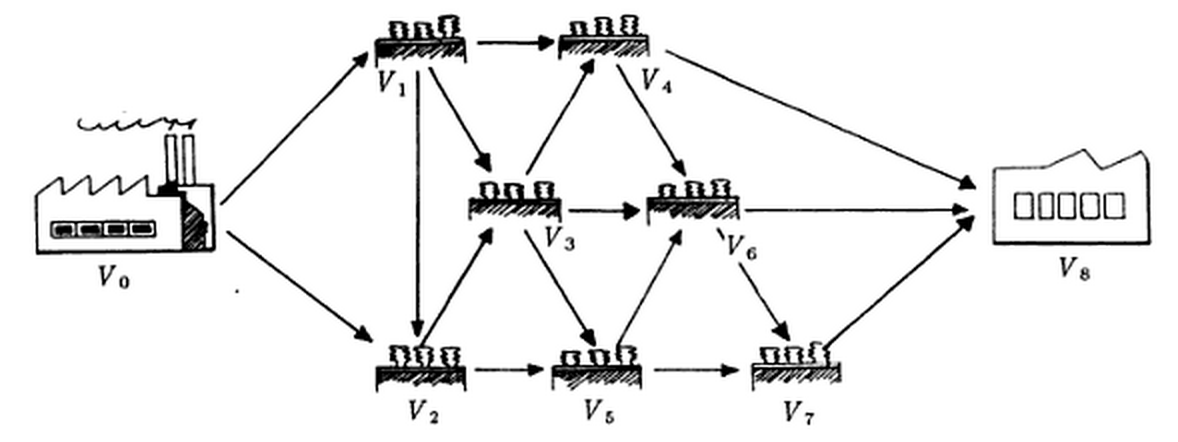
\includegraphics[width=0.8\textwidth]{energiefluss}

\end{figure}

Ein anderes Optimierungsproblem ergibt sich, wenn elektrischer Strom einer vorgegebenen St�rke kostenoptimal durch ein Netz (von der Quelle zur Senke) geschickt werden soll und die Kosten aus Spannungsverlusten resultieren, die jeweils proportional zu den Stromst�rken in den Leitungen sind.

Bezeichnen wir mit $x_{ij}$ den von $V_i$ nach $V_j$ flie�enden Strom\footnote{Genauer: Unter der Voraussetzung, dass die Kante von $v_i$ nach $v_j$ vorhanden ist, bezeichnen wir mir $x_{ij}$ den �ber diese Kante von $v_i$ nach $v_j$ flie�enden Strom.}, so erhalten wir neben einer Zielfunktion in der bekannten linearen Form f�r jeden Verteilerknoten die Bedingung, dass die hineinflie�ende gleich der herausflie�enden Menge ist. Beispielsweise gilt f�r $V_3$
\[
x_{13} + x_{23} - x_{34} - x_{35} - x_{36} = 0.
\]

Eine entsprechende Beziehung gilt f�r die Quelle und die Senke. Die aus der Quelle herausflie�ende Menge $w$ ist gerade gleich der in die Senke hineinflie�enden Menge, da in den Verteilerknoten nichts \enquote{verlorengeht}. F�r das obige Beispiel erhalten wir damit
\[
x_{01} + x_{02} = w = x_{48} + x_{68} + x_{78}.
\]

Neben diesen sogenannten Knotenbedingungen\index{Knotenbedingungen} sind noch die Maximalbelastungen der Leitungen als (obere) Kapazit�tsschranken\index{Kapazit�tsschranke}\index{Schranke!Kapazit�ts-} zu beachten, d.h., f�r die St�rke $x_{ij}$ des von $V_i$ nach $V_j$ flie�enden Stroms gilt
\[
0 \leq x_{ij} \leq \kappa_{ij},
\] 
wobei als untere Kapazit�tsschranke 0 verwendet wird.

Den oben skizzierten Zielfunktionen und Nebenbedingungen ist zu entnehmen, dass wir es sowohl bei der Bestimmung eines \textit{Flusses maximaler St�rke}\index{Fluss!maximaler St�rke} (Maximierung von $w$) als auch bei der Berechnung eines \textit{kostenoptimalen Flusses}\index{kostenoptimaler Fluss}\index{Fluss!kostenoptimaler} vorgegebener St�rke mit sehr speziell strukturierten linearen Problemen zu tun haben, f�r die auch spezielle Verfahren entwickelt worden sind\footnote{Fl�sse maximaler St�rke werden im Rahmen der Vorlesung noch genauer behandelt werden.}.

Eingesetzt werden derartige Modelle und Verfahren seit Anfang der 60er Jahre in einem breiten Spektrum von Anwendungen. Bereits zu dieser Zeit wurde z.B. vom Automobilhersteller Chrysler in den USA ein Planungsinstrument f�r die kosteng�nstigste Belieferung der H�ndler von den Produktionsst�tten aus entwickelt (vgl. SHAPIRO (1984), Kapitel 5). Von 10 Werken aus sollen etwa 5000 H�ndler in den USA und in Kanada �ber ein gegebenes Vertriebsnetz beliefert werden. In Erweiterung der in Abb. 0.2.3 dargestellten Situation haben wir es mit einer Vielzahl von Quellen und Senken zu tun, was sich jedoch ohne Schwierigkeiten auf den Fall einer Senke und einer Quelle zur�ckf�hren l�sst. Ferner kann im Rahmen dieses Modells auch ber�cksichtigt werden, dass die Produktionskosten pro Fahrzeug in den einzelnen Werken unterschiedlich sein k�nnen und Beschr�nkungen hinsichtlich des Produktionsaussto�es bestehen.


%------------------------------------------------------------ end

%\bigskip

%Neben den beiden im Beispiel angesprochenen Problemen (\textit{Fluss maximaler St�rke} und \textit{kostenoptimaler Fluss}) gibt es eine Reihe von weiteren Netzwerkproblemen, die sich auf nat�rliche Art als LP-Probleme formulieren lassen. Hier noch ein weiteres Beispiel: das \textit{Problem der multiplen Warenfl�sse} (aus Cormen et al, Seite 876f).
%
%\bigskip

%------------------------------------------------------------ begin

%\subsubsection{Multiple Warenfl�sse}
%\index{multiple Warenfl�sse}\index{Warenfl�sse!multiple}\index{Problem!der multiplen Warenfl�sse}
%
%Als abschlie�endes Beispiel betrachten wir ein weiteres Flussproblem. Nehmen Sie an, die Firma Lucky Puck aus Abschnitt 26.1 w�rde beschlie�en, ihre Produktpalette zu erweitern und nicht nur Hockeypucks, sondern auch Hockeyschl�ger und Hockeyhelme herzustellen. Jedes Teil wird in einer eigenen Fabrik hergestellt, hat sein eigenes Warenlager und muss jeden Tag von der Fabrik zum Warenlager transportiert werden. Die Schl�ger werden in Vancouver hergestellt und m�ssen nach Saskatoon gebracht werden, die Helme werden in Edmonton hergestellt und nach Regina transportiert. Die Kapazit�t des Transportnetzwerks �ndert sich jedoch nicht und die verschiedenen Elemente, d.h. die Waren, m�ssen sich das gleiche Netzwerk teilen.
%
%Dieses Beispiel ist eine Instanz des \textit{Problems multipler Warenfl�sse}. Bei diesem Problem haben wir wieder einen gerichteten Graphen $G=(V,E)$ gegeben, in dem jeder Kante $(u,v) \in E$ eine nichtnegative Kapazit�t $c(u,v) \geq 0$ zugeordnet ist. Wie beim maximalen-Fluss-Problem setzen wir implizit voraus, dass $c(u,v)=0$ gilt, wenn $(u,v) \notin E$ und der Graph keine antiparallelen Kanten enth�lt. Zus�tzlich haben wir $k$ verschiedene Waren $K_1, \ldots, K_k$ gegeben, wobei wir die Ware $i$ durch das Tripel $K_i=(s_i,t_i,d_i)$ spezifizieren. $s_i$ ist die Quelle f�r Ware $i$, $t_i$ die Senke f�r Ware $i$ und $d_i$ der Bedarf f�r Ware $i$, also der gew�nschte Wert des Flusses f�r die Ware von $s_i$ nach $t_i$. Wir definieren einen Fluss f�r die Ware $i$, den wir mit $f_i$ bezeichnen (so dass $f_{iuv}$ der Fluss der Ware $i$ von Knoten $u$ nach Knoten $v$ ist), als eine reellwertige Funktion, die der Flusserhaltung und den Kapazit�tsbeschr�nkungen gen�gt. Wir definieren nun $f_{uv}$, den \textit{Aggregat-Fluss}, als die Summe der einzelnen Warenfl�sse, d.h. $f_{uv} = \sum\limits_{i=1}^{k}{f_{iuv}}$. Der Aggregat-Fluss entlang der Kante $(u,v)$ darf nicht gr��er als die Kapazit�t der Kante $(u,v)$ sein. 
%
%Wir versuchen in diesem Problem nicht, eine Zielfunktion zu minimieren; wir wollen nur pr�fen, ob ein solcher Fluss existiert. Daher schreiben wir ein lineares Programm, das als Zielfunktion die \enquote{Null}-Funktion hat:
%
%minimiere 0 \\
%unter den Nebenbedingungen
%\begin{alignat*}{3}
%\sum\limits_{i=1}^{k}{f_{iuv}} &\leq c(u,v) 
%&&\quad \text{f�r alle } u,v \in V; \\
%\sum\limits_{v \in V}{f_{iuv}} - \sum\limits_{v \in V}{f_{ivu}} &= 0 
%&&\quad \text{f�r alle } i=1,\ldots,k \text{ und f�r alle } u \in V \setminus \bigl\{ s_i,t_i \bigr\}; \\
%\sum\limits_{v \in V}{f_{is_iv}} - \sum\limits_{v \in V}{f_{ivs_i}} &= d_i 
%&&\quad \text{f�r alle } i=i,\ldots,k; \\
%f_{iuv} &\geq 0 
%&&\quad \text{f�r alle } u,v \in V \text{ und f�r alle } i=1,\ldots,k.
%\end{alignat*}
%
%Der einzige bekannte Algorithmus mit polynomieller Laufzeit f�r dieses Problem besteht darin, das Problem als lineares Programm zu formulieren und dieses durch einen Algorithmus zur L�sung linearer Programme mit polynomieller Laufzeit zu l�sen.

%------------------------------------------------------------ end


%------------------------------------------------------------------------------%
% Abschnitt:                                                                   %
% "Das Rucksackproblem (Knapsack Problem)"                                     %
%------------------------------------------------------------------------------%

\section{Das Rucksackproblem (Knapsack Problem)}
\index{Rucksackproblem}\index{Problem!Rucksack-}\index{Knapsack-Problem}

Die folgende Darstellung findet sich in
\begin{itemize}
\item S. Dasgupta, C. Papadimitriou, U. Vazirani: \textit{Algorithms}. McGraw Hill (2008).
\end{itemize}

\bigskip

%------------------------------------------------------------ begin

During a robbery, a burglar finds much more loot than he had expected and has to decide what to take. His bag (or \foreignquote{english}{knapsack}) will hold a total weight of at most $W$ pounds. There are $n$ items to pick from, of weight $w_1, \ldots, w_n$ and dollar value $v_1, \ldots, v_n$. What's the most valuable combination of items he can fit into his bag?\footnote{If this application seems frivolous, replace \foreignquote{english}{weight} with \foreignquote{english}{CPU time} and \foreignquote{english}{only $W$ pounds can be taken} with \foreignquote{english}{only $W$ units of CPU time are available.} Or use \foreignquote{english}{bandwidth} in place of \foreignquote{english}{CPU time,} etc. The knapsack problem generalizes a wide variety of resource-constrained selection tasks.}

For instance, take $W = 10$ and
\begin{center}
\begin{tabular}{c|cr}
Item & Weight & Value \\ \hline
1 & 6 & \$30 \\
2 & 3 & \$14 \\
3 & 4 & \$16 \\
4 & 2 & \$9
\end{tabular}
\end{center}

There are two versions of this problem. If there are unlimited quantities of each item available, the optimal choice is to pick item 1 and two of item 4 (total: \$48). On the other hand, if there is one of each item (the burglar has broken into an art gallery, say), then the optimal knapsack contains items 1 and 3 (total: \$46).

%------------------------------------------------------------ end

\bigskip

Wir formulieren das beschriebene Problem wie folgt:

\underline{\textit{Version 1} (\enquote{jeder Gegenstand nur einmal vorhanden})}:
\begin{align*}
\begin{alignedat}{6}
& \text{maximiere } & 30x_1 &\ + &\ 14x_2 &\ + &\ 16x_3 &\ + &\ 9x_4 \\
& \rlap{unter den Nebenbedingungen} & & & & & & & \\
&& 6x_1 &\ + &\ 3x_2 &\ + &\ 4x_3 &\ + &\ 2x_4 &\ \leq &\ 10 \\
&& & & & & & & & & \llap{$x_1,x_2,x_3,x_4 \in \bigl\{ 0,1 \bigr\}$}
\end{alignedat}
\end{align*}


\underline{\textit{Version 2} (\enquote{beliebig viele Exemplare von jedem Gegenstand vorhanden})}:
\begin{align*}
\begin{alignedat}{6}
& \text{maximiere } & 30x_1 &\ + &\ 14x_2 &\ + &\ 16x_3 &\ + &\ 9x_4 \\
& \rlap{unter den Nebenbedingungen} & & & & & & & \\
&& 6x_1 &\ + &\ 3x_2 &\ + &\ 4x_3 &\ + &\ 2x_4 &\ \leq &\ 10 \\
&& & & & & & & \llap{$x_1,x_2,x_3,x_4$} &\ \geq &\ 0 \\
&& & & & & & & \llap{$x_1,x_2,x_3,x_4$} &\ \in &\ \Z
\end{alignedat}
\end{align*}

Version 1 wird f�r uns die wichtigere sein. \textit{Offensichtlich handelt es sich weder bei Version 1 noch bei Version 2 um ein LP-Problem}: Bedingungen der Art $x_1,x_2,x_3,x_4 \in \bigl\{ 0,1 \bigr\}$ bzw. $x_1,x_2,x_3,x_4 \in \Z$ sind in LP-Problemen ja gar nicht vorgesehen.

\pagebreak
Bei Version 2 handelt es sich um ein \textit{Ganzzahliges Lineares Programmierungsproblem}\index{Ganzzahliges Lineares Programmierungsproblem}\index{Problem!Ganzzahliges Lineares Programmierungs-} (engl. \textit{integer linear programming problem}, kurz: \textit{ILP-Problem}\index{ILP-Problem}\index{Problem!ILP-}). Allgemein gilt: Ein Optimierungsproblem wird \textit{Ganzzahliges Lineares Programmierungsproblem} oder \textit{ILP-Problem} genannt, falls Folgendes erf�llt ist:
\begin{itemize}
	\item F�r jede Variable $x_i$ wird $x_i \in \Z$ gefordert.
	\item L�sst man s�mtliche Bedingungen $x_i \in \Z$ weg, so liegt ein LP-Problem vor.
\end{itemize}

Bei einem Ganzzahligen Linearen Programmierungsproblem d�rfen die Werte der Variablen also nur ganze Zahlen sein. Bei Version 1 sind die M�glichkeiten sogar noch weiter eingeschr�nkt: Die Variablen d�rfen nur einen der Werte 0 oder 1 annehmen. Man spricht von einem \textit{0,1-Problem}\index{0,1-Problem}\index{Problem!0,1-} (oder von einem \textit{bin�ren Problem}\index{bin�res Problem}\index{Problem!bin�res}).

Wenn man in der Version 2 die Bedingungen $x_1,x_2,x_3,x_4 \in \Z$ wegl�sst, so gelangt man in der Tat zu einem LP-Problem. (Nebenbei: Wie lautet die optimale L�sung dieses LP-Problems?) Das entstehende LP-Problem nennt man �brigens die \textit{LP-Relaxation} des urspr�nglichen Problems\footnote{Allgemein gilt: L�sst man in einem ILP-Problem s�mtliche Bedingungen $x_i \in \Z$ weg, so nennt man das entstehende LP-Problem die \textit{LP-Relaxation}\index{LP-Relaxation} des urspr�nglichen Problems.}.

Allgemein lautet das Rucksackproblem\index{Rucksackproblem}\index{Problem!Rucksack-} wie folgt:

\underline{\textit{Rucksackproblem} (\textit{Version 1})}:\label{page:6:1}
\begin{align*}
\begin{alignedat}{6}
& \text{maximiere } & c_1x_1 &\ + &\ \ldots &\ + &\ c_nx_n & & & \\
& \rlap{unter den Nebenbedingungen} & & & & & & & & \\
&& a_1x_1 &\ + &\ \ldots &\ + &\ a_nx_n &\ \leq &\ b & \\
&& & & & & & & \llap{$x_i \in \bigl\{ 0,1 \bigr\}$} & \qquad (i=1,\ldots,n)
\end{alignedat}
\end{align*}

\underline{\textit{Rucksackproblem} (\textit{Version 2})}:
\begin{align*}
\begin{alignedat}{6}
& \text{maximiere } & c_1x_1 &\ + &\ \ldots &\ + &\ c_nx_n & & & \\
& \rlap{unter den Nebenbedingungen} & & & & & & & & \\
&& a_1x_1 &\ + &\ \ldots &\ + &\ a_nx_n &\ \leq &\ b & \\
&& & & & & \llap{$x_i$} &\ \geq &\  0 & \qquad (i=1,\ldots,n) \\
&& & & & & \llap{$x_i$} &\ \in &\ \Z & \qquad (i=1,\ldots,n)
\end{alignedat}
\end{align*}



Bei zahlreichen ganzzahligen oder bin�ren Problemen handelt es sich um \textit{NP-schwere Probleme} -- das Rucksackproblem ist da keine Ausnahme (weder in der einen noch in der anderen Version).

�brigens: Die Bedingung $x_i \in \bigl\{ 0,1 \bigr\}$ kann ersetzt werden durch $0 \leq x_i \leq 1$, $x_i \in \Z$. Man kann also jedes $0,1$-Problem in ein Ganzzahliges Lineares Programmierungsproblem umschreiben. Anders gesagt: Bei den $0,1$-Problemen handelt es sich um spezielle ILP-Probleme.

Wir halten noch einmal ausdr�cklich fest: \textit{Bei beiden Versionen des Rucksackproblems handelt es sich \textbf{nicht} um ein LP-Problem, sondern um ein ILP-Problem.} F�r ILP-Probleme kommen �brigens g�nzlich andere Methoden zum Einsatz als f�r LP-Probleme; einen ersten Einblick in diese Methoden findet man beispielsweise im Lehrbuch von D. Bertsimas und J. N. Tsitsiklis. 




\section{Cutting Paper Rolls}

Die Liste der Anwendungsm�glichkeiten Linearer Programmierung ist lang und wir k�nnen hier nat�rlich l�ngst nicht alles besprechen. Wir pr�sentieren deshalb nur noch ein Beispiel, in dem es um ein \textit{Verschnittproblem}\index{Verschnittproblem}\index{Problem!Verschnitt-} geht. Derartige Probleme treten sehr h�ufigen in industriellen Fertigungsprozessen auf: Es geht darum, Rohmaterial optimal zu nutzen.

\pagebreak
Der folgende Text stammt aus dem Buch
\begin{itemize}
\item Matou\v{s}ek/G�rtner: \textit{Understanding and Using Linear Programming}.
\end{itemize}

% begin

Here we have another industrial problem, and the application of linear programming is quite nonobvious. Moreover, we will naturally encounter an integrality constraint, which will bring us to the topic of the next chapter.

A paper mill manufactures rolls of paper of a standard width 3 meters. But customers want to buy paper rolls of shorter width, and the mill has to cut such rolls from the 3 m rolls. One 3 m roll can be cut, for instance, into two rolls 93 cm wide, one roll of width 108 cm, and a rest of 6 cm (which goes to waste).

Let us consider an order of
\begin{itemize}
\item 97 rolls of width 135 cm,
\item 610 rolls of width 108 cm,
\item 395 rolls of width 93 cm, and
\item 211 rolls of width 42 cm.
\end{itemize}

What is the smallest number of 3 m rolls that have to be cut in order to satisfy this order, and how should they be cut?

In order to engage linear programming one has to be generous in introducing variables. We write down all of the requested widths: 135 cm, 108 cm, 93 cm, and 42 cm. Then we list all possibilities of cutting a 3 m paper roll into rolls of some of these widths (we need to consider only possibilities for which the wasted piece is shorter than 42 cm):
\begin{align*}
P_1:&\quad 2 \cdot 135 &P_7: &\quad 108 + 93 + 2 \cdot 42 \\
P_2:&\quad 135 + 108 + 42 &P_8: &\quad 108 + 4 \cdot 42 \\
P_3:&\quad 135 + 93 + 42 &P_9: &\quad 3 \cdot 93 \\
P_4:&\quad 135 + 3 \cdot 42 &P_{10}: &\quad 2 \cdot 93 + 2 \cdot 42 \\
P_5:&\quad 2 \cdot 108 + 2 \cdot 42 &P_{11}: &\quad 93 + 4 \cdot 42 \\
P_6:&\quad 108 + 2 \cdot 93 &P_{12}: &\quad 7 \cdot 42
\end{align*}

For each possibility $P_j$ on the list we introduce a variable $x_j \geq 0$ representing the number of rolls cut according to that possibility. We want to minimize the total number of rolls cut, i.e., $\sum\limits_{j=1}^{12}{x_j}$, in such a way that the customers are satisfied. For example, to satisfy the demand for 395 rolls of width 93 cm we require
\[
x_3 + 2x_6 + x_7 + 3x_9 + 2x_{10} + x_{11} \geq 395.
\]

For each of the widths we obtain one constraint.

For a more complicated order, the list of possibilities would most likely be produced by computer. We would be in a quite typical situation in which a linear program is not entered \foreignquote{english}{by hand,} but rather is generated by some computer program. More-advanced techniques even generate the possibilities \foreignquote{english}{on the fly,} during the solution of the linear program, which may save time and memory considerably. See the entry \foreignquote{english}{column generation} in the glossary or Chv�tal's book cited in Chapter 9, from which this example is taken.

The optimal solution of the resulting linear program has $x_1 = 48.5$, $x_5 = 206.25$, $x_6 = 197.5$, and all other components 0. In order to cut 48.5 rolls according to the possibility $P_1$, one has to unwind half of a roll. Here we need more information about the technical possibilities of the paper mill: Is cutting a fraction of a roll technically and economically feasible? If yes, we have solved the problem optimally. If not, we have to work further and somehow take into account the restriction that only feasible solutions of the linear program with integral $x_i$ are of interest. This is not at all easy in general, and it is the subject of Chapter 3.

% end

\bigskip

In Chv�tals Buch wird dieses Beispiel noch wesentlich genauer behandelt (Abschnitt 13: The Cutting-Stock Problem). Auch im bereits �fter zitierten Buch von Neumann und Morlock findet sich einiges �ber verwandte Probleme, beispielsweise �ber so genannte \textit{2-dimensionale Verschnittprobleme}\index{Verschnittproblem}\index{Problem!Verschnitt-}\index{Verschnittproblem!2-dimensionales}\index{2-dimensionales Verschnittproblem}.

Was unter einem 2-dimensionalen Verschnittproblem zu verstehen ist, wollen wir hier nur andeuten, indem wir die folgende Zeichnung aus dem Buch von Neumann/Morlock wiedergeben:

\begin{figure}[H]

\centering
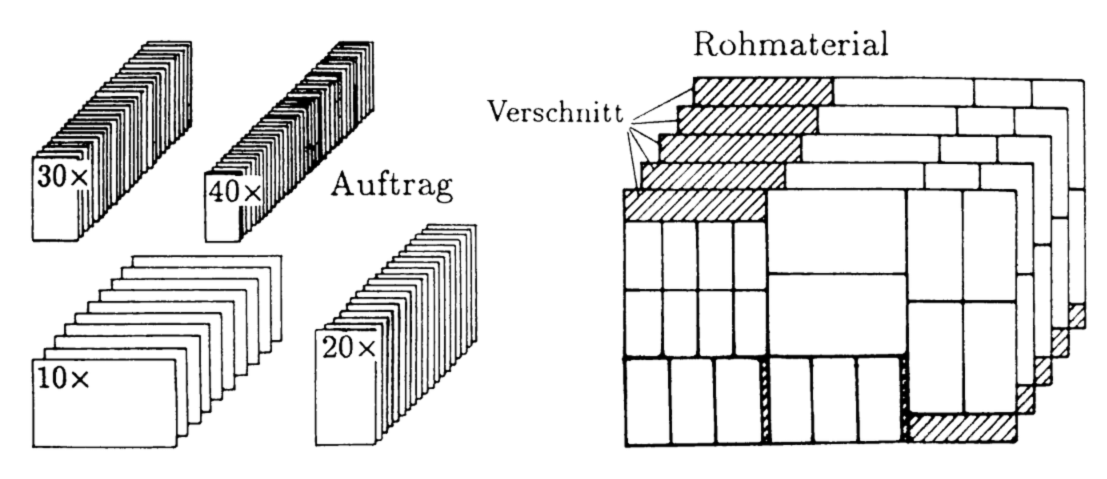
\includegraphics[width=0.8\textwidth]{verschnitt}

\end{figure}


%------------------------------------------------------------------------------%
% Skript zu:                                                                   %
% "Optimierung f�r Studierende der Informatik"                                 %
% ============================================                                 %
%                                                                              %
% Kapitel 07:                                                                  %
% "Dualit�t"                                                                   %
%                                                                              %
% in LaTeX gesetzt von:                                                        %
% Steven K�hler                                                                %
%                                                                              %
% Version:                                                                     %
% 2017-01-31                                                                   %
%------------------------------------------------------------------------------%


\chapter{Dualit�t}\label{chapter:7}
\index{Dualit�t}


%------------------------------------------------------------------------------%
% Abschnitt:                                                                   %
% "Motivation: obere Schranken f�r den optimalen Wert"                         %
%------------------------------------------------------------------------------%

\section{Motivation: obere Schranken f�r den optimalen Wert}
\label{section:7:1}


Wir betrachten das folgende LP-Problem in Standardform:
\begin{align}
\begin{alignedat}{6}
\label{eq:7:1}
& \text{maximiere } & 4x_1 &\ + &\ x_2 &\ + &\ 5x_3 &\ + &\ 3x_4 & & \\
& \rlap{unter den Nebenbedingungen} & & & & & & & & & \\
&&  x_1 &\ - &\  x_2 &\ - &\  x_3 &\ + &\ 3x_4 &\ \leq &\  1\ \\
&& 5x_1 &\ + &\  x_2 &\ + &\ 3x_3 &\ + &\ 8x_4 &\ \leq &\ 55\ \\
&& -x_1 &\ + &\ 2x_2 &\ + &\ 3x_3 &\ - &\ 5x_4 &\ \leq &\  3\ \\
&& & & & & & & \llap{$x_1, x_2, x_3, x_4$} &\ \geq &\ 0.
\end{alignedat}
\end{align}


Anstatt das Problem zu l�sen, wollen wir versuchen, m�glichst gute \textit{obere Schranken}\index{obere Schranke}\index{Schranke!obere} f�r den optimalen Zielfunktionswert $z^*$ unmittelbar am gegebenen LP-Problem abzulesen.

Beispielsweise k�nnte man die zweite Nebenbedingung mit 2 multiplizieren:
\[
10x_1 + 2x_2+6x_3+16x_4 \leq 110.
\]

Es folgt, dass f�r jede zul�ssige L�sung gilt:
\[
4x_1 + x_2 + 5x_3 + 3x_4 \leq 10x_1 + 2x_2 + 6x_3 + 16x_4 \leq 110.
\]

Da dies f�r jede zul�ssige L�sung gilt, gilt es insbesondere auch f�r jede optimale L�sung. Wir haben somit $z^* \leq 110$ erhalten.

Stellen wir uns etwas geschickter an, so k�nnen wir diese obere Schranke f�r $z^*$ noch verbessern. Beispielsweise erh�lt man $z^* \leq \frac{275}{3}$, wenn man die zweite Nebenbedingung nicht mit 2, sondern mit $\frac{5}{3}$ multipliziert; in diesem Fall ergibt sich f�r jede zul�ssige L�sung:
\[
4x_1 + x_2 + 5x_3 + 3x_4 \leq \frac{25}{3}x_1 + \frac{5}{3}x_2 + 5x_3 + \frac{40}{3}x_4 \leq \frac{275}{3}.
\]

Also (insbesondere) $z^* \leq \frac{275}{3}$.

Mit etwas Eingebung und Fantasie k�nnen wir diese Schranke noch weiter verbessern. Addiert man beispielsweise die zweite und die dritte Nebenbedingung, so erh�lt man
\[
4x_1 + 3x_2 + 6x_3 + 3x_4 \leq 58;
\]

es folgt $z^* \leq 58$.

Wir wollen nun systematisch vorgehen und eine Strategie zum Auffinden von oberen Schranken f�r $z^*$ beschreiben: \textit{Wir bilden eine Linearkombination der Nebenbedingungen\index{Linearkombination von Nebenbedingungen}\index{Nebenbedingungen!Linearkombination von}, d.h., wir nehmen die erste Nebenbedingung mit einer Zahl $y_1$ mal, die zweite Nebenbedingung mit $y_2$, die dritte mit $y_3$; danach addieren wir die erhaltenen Ungleichungen}.

\textit{Dabei setzen wir voraus, dass $y_1 \geq 0$, $y_2 \geq 0$ und $y_3 \geq 0$ gilt}. (In unseren obigen Betrachtungen, die zu $z^* \leq \frac{275}{3}$ bzw. zu $z^* \leq 58$ gef�hrt haben, galt $y_1=0$, $y_2=\frac{5}{3}$, $y_3 = 0$ bzw. $y_1=0$, $y_2=y_3=1$.)

Im allgemeinen Fall (d.h. mit beliebigen $y_1,y_2,y_3 \geq 0$) erh�lt man
\begin{equation}
\label{eq:7:2}
\Bigl( y_1+5y_2-y_3\Bigr)x_1 + \Bigl( -y_1+y_2+2y_3\Bigr)x_2 + \Bigl( -y_1+3y_2+3y_3 \Bigr)x_3 + \Bigl( 3y_1+8y_2-5y_3\Bigr)x_4
 \leq y_1 + 55y_2 + 3y_3.
\end{equation}

Nun m�chte man erreichen, dass die linke Seite von (\ref{eq:7:2}) eine obere Schranke f�r die Zielfunktion 
\[
z = 4x_1+x_2+5x_3+3x_4
\]
ergibt. Dies ist gewiss der Fall, wenn Folgendes gilt:
\begin{align*}
\begin{alignedat}{4}
 y_1 &\ + &\ 5y_2 &\ - &\  y_3 &\ \geq &\ 4\ \\
-y_1 &\ + &\  y_2 &\ + &\ 2y_3 &\ \geq &\ 1\ \\
-y_1 &\ + &\ 3y_2 &\ + &\ 3y_3 &\ \geq &\ 5\ \\
3y_1 &\ + &\ 8y_2 &\ - &\ 5y_3 &\ \geq &\ 3.
\end{alignedat}
\end{align*}

Wenn also die Faktoren $y_i$ nichtnegativ sind und diese 4 Ungleichungen erf�llt sind, so k�nnen wir sicher sein, dass jede zul�ssige L�sung $(x_1,x_2,x_3,x_4)$ die Ungleichung
\[
4x_1 + x_2 + 5x_3 + 3x_4 \leq y_1 + 55y_2 + 3y_3
\]
erf�llt. Da diese Ungleichung f�r alle zul�ssigen L�sungen gilt, also insbesondere auch f�r eine optimale L�sung, erhalten wir
\[
z^* \leq y_1 + 55y_2 + 3y_3.
\]

Wir m�chten gerne, dass diese obere Schranke f�r $z^*$ m�glichst nahe bei $z^*$ liegt. \textit{Damit sind wir beim folgenden Minimierungsproblem angelangt}:
\begin{align*}
\begin{alignedat}{5}
& \text{minimiere } & y_1 &\ + &\ 55y_2 &\ + &\ 3y_3 & & \\
& \rlap{unter den Nebenbedingungen} & & & & & & & \\
&&  y_1 &\ + &\ 5y_2 &\ - &\  y_3 &\ \geq &\ 4\ \\
&& -y_1 &\ + &\  y_2 &\ + &\ 2y_3 &\ \geq &\ 1\ \\
&& -y_1 &\ + &\ 3y_2 &\ + &\ 3y_3 &\ \geq &\ 5\ \\
&& 3y_1 &\ + &\ 8y_2 &\ - &\ 5y_3 &\ \geq &\ 3\ \\
&& & & & & \llap{$y_1,y_2,y_3$} &\ \geq &\ 0. 
\end{alignedat}
\end{align*}



Das so erhaltene LP-Problem nennt man das \textit{duale Problem}\index{duales Problem}\index{Problem!duales} des urspr�nglichen Problems\footnote{Statt \enquote{urspr�ngliches Problem} sagt man auch \textit{primales Problem}\index{primales Problem}\index{Problem!primales}.}.

\section{Das duale Problem}
\label{section:7:2}

Wir betrachten nun den allgemeinen Fall. Gegeben sei ein LP-Problem in Standardform:
\begin{align}
\tag{P}
\begin{alignedat}{4}
& \text{maximiere } & \sum\limits_{j=1}^{n}{c_jx_j} & & & \\
& \rlap{unter den Nebenbedingungen} & & & & \\
&& \sum\limits_{j=1}^{n}{a_{ij}x_j} &\ \leq &\ b_i & \qquad (i=1,\ldots,m) \\
&&                              x_j &\ \geq &\   0 & \qquad (j=1,\ldots,n).
\end{alignedat}
\end{align}

Dann nennt man das folgende Problem das \textit{duale Problem} zu (P):
\begin{align}
\tag{D}
\begin{alignedat}{4}
& \text{minimiere } & \sum\limits_{i=1}^{m}{b_iy_i} & & & \\
& \rlap{unter den Nebenbedingungen} & & & & \\
&& \sum\limits_{i=1}^{m}{a_{ij}y_i} &\ \geq &\ c_j & \qquad (j=1,\ldots,n) \\
&&                              y_i &\ \geq &\   0 & \qquad (i=1,\ldots,m).
\end{alignedat}
\end{align}

\textit{Man beachte}: Das Duale\index{Duales} eines Maximierungsproblems ist ein Minimierungsproblem; jeder der $m$ \textit{primalen Nebenbedingungen}\index{primale Nebenbedingung}\index{Nebenbedingungen!primale}
\[
\sum\limits_{j=1}^{n}{a_{ij}x_j} \leq b_i
\]

entspricht eine \textit{duale Variable}\index{duale Variable}\index{Variable!duale} $y_i\ (i=1,\ldots,m)$; umgekehrt gilt: Jeder der $n$ \textit{dualen Nebenbedingungen}\index{duale Nebenbedingung}\index{Nebenbedingungen!duale}
\[
\sum\limits_{i=1}^{m}{a_{ij}y_i} \geq c_j
\]

entspricht eine \textit{primale Variable}\index{primale Variable}\index{Variable!primale} $x_j\ (j=1\ldots,n)$; die Koeffizienten $c_j$ der primalen Zielfunktion tauchen im dualen Problem als rechte Seite auf; Entsprechendes gilt umgekehrt auch f�r die Koeffizienten $b_i$.

Besonders kurz kann man das alles aufschreiben, wenn man \textit{Matrixschreibweise}\index{Matrixschreibweise} verwendet; dann lauten das primale Problem (P) und das duale Problem (D) wie folgt:

\begin{SKBox}
\textbf{Primales Problem}.
\begin{align}
\tag{P}
\begin{alignedat}{3}
& \text{maximiere } & c^Tx & & \\
& \rlap{unter den Nebenbedingungen} & & \\
&& Ax &\ \leq &\ b \\
&&  x &\ \geq &\ 0
\end{alignedat}
\end{align}
\end{SKBox}

\begin{SKBox}
\textbf{Duales Problem}.
\begin{align}
\tag{D}
\begin{alignedat}{3}
& \text{minimiere } & b^Ty & & \\
& \rlap{unter den Nebenbedingungen} & & \\
&& A^Ty &\ \geq &\ c \\
&&    y &\ \geq &\ 0
\end{alignedat}
\end{align}
\end{SKBox}

Hierin ist 
\[
c^T = (c_1,\ldots,c_n), \quad
b^T = (b_1,\ldots,b_m), \quad
x = \begin{pmatrix} x_1 \\ \vdots \\ x_n \end{pmatrix}, \quad
y = \begin{pmatrix} y_1 \\ \vdots \\ y_m \end{pmatrix}, \quad
A = \begin{pmatrix} a_{11} & \ldots & a_{1n} \\ \vdots & \ddots & \vdots \\ a_{m1} & \ldots & a_{mn} \end{pmatrix};
\]

$0$ bezeichnet in (P) den Nullvektor der L�nge $n$ und in (D) den Nullvektor der L�nge $m$; die Ungleichungen sind komponentenweise zu lesen, beispielsweise bedeutet $y \geq 0$ dasselbe wie $y_i \geq 0$ f�r $i=1,\ldots,m$.

Wie bereits in unserem Beispiel beobachtet, liefert jede zul�ssige L�sung des dualen Problems eine \textit{obere Schranke} f�r den optimalen Wert des primalen Problems. 

\begin{Definition}[Feststellung]
Ist $(x_1,\ldots,x_n)$ eine primale zul�ssige L�sung\index{primale zul�ssige L�sung}\index{L�sung!primale zul�ssige}\index{zul�ssige L�sung!primale} und $(y_1,\ldots,y_m)$ eine duale zul�ssige L�sung\index{duale zul�ssige L�sung}\index{L�sung!duale zul�ssige}\index{zul�ssige L�sung!duale}\footnotemark, so gilt
\begin{equation}
\label{eq:7:3}
\sum\limits_{j=1}^{n}{c_jx_j} \leq \sum\limits_{i=1}^{m}{b_iy_i}.
\end{equation}
\end{Definition}

\footnotetext{\enquote{Primale zul�ssige L�sung} bedeutet nat�rlich \enquote{zul�ssige L�sung des primalen Problems}; analog: \enquote{duale zul�ssige L�sung}. Die Bezeichnungen $c_j$ und $b_i$ seien wie in (P) und (D).}

Die wichtige Feststellung (\ref{eq:7:3}) wird \textit{schwache Dualit�t}\index{schwache Dualit�t}\index{Dualit�t!schwache} genannt. Der Beweis von (\ref{eq:7:3}) ist sehr kurz.

\textbf{Beweis}.
\[
\sum\limits_{j=1}^{n}{c_jx_j} \leq \sum\limits_{j=1}^{n}{\left( \sum\limits_{i=1}^{m}{a_{ij}y_i} \right) x_j}
= \sum\limits_{i=1}^{m}{\left( \sum\limits_{j=1}^{n}{a_{ij}x_j} \right) y_i} \leq \sum\limits_{i=1}^{m}{b_iy_i}. \quad \Box
\]

Dasselbe in Matrixschreibweise:
\[
c^Tx \leq {\Bigl( A^Ty \Bigr)}^Tx = \Bigl( y^TA \Bigr) x = y^T \Bigl( Ax \Bigr) \leq y^Tb = b^Ty.
\]

\textit{Die Beziehung (\ref{eq:7:3}) (\enquote{schwache Dualit�t}) ist sehr n�tzlich}: Falls wir irgendwo her eine primale zul�ssige L�sung $(x_1^*, \ldots, x_n^*)$ und eine duale zul�ssige L�sung $(y_1^*, \ldots, y_m^*)$ haben und falls
\begin{equation}
\label{eq:7:4}
\sum\limits_{j=1}^{n}{c_jx_j^*} = \sum\limits_{i=1}^{m}{b_iy_i^*}
\end{equation}
gilt, so k�nnen wir sicher sein, dass $(x_1^*, \ldots, x_n^*)$ eine optimale L�sung des primalen Problems und $(y_1^*, \ldots, y_m^*)$ eine optimale L�sung des dualen Problems ist. (Wieso n�mlich?)

\textbf{Beispiel}. Wir betrachten das LP-Problem (\ref{eq:7:1}), das uns bereits am Anfang dieses Abschnitts zur Illustration diente: $x_1=0$, $x_2=14$, $x_3=0$, $x_4=5$ ist eine zul�ssige L�sung dieses Problems -- davon k�nnen wir uns leicht �berzeugen. Wir brauchen die Zahlen $x_1=0$, $x_2=14$, $x_3=0$, $x_4=5$ ja nur in (\ref{eq:7:1}) einzusetzen.

Ich behaupte nun: \textit{Die Zahlen $x_1=0$, $x_2=14$, $x_3=0$ und $x_4=5$ bilden sogar eine optimale L�sung von (\ref{eq:7:1})}. Stellen wir uns vor, das Sie dies bezweifeln. \textit{Wie kann ich Sie schnell davon �berzeugen, dass ich Recht habe?}

\textit{Hier ist die Antwort}: Ich pr�sentiere Ihnen zus�tzlich die Zahlen 
\[
y_1=11,\quad y_2=0 \quad\text{und}\quad y_3=6,
\]
die ich \enquote{magische Zahlen} nenne, da ich mit ihrer Hilfe s�mtliche Zweifel zum Verschwinden bringe.

Bei diesen Zahlen handelt es sich um eine zul�ssige L�sung des dualen Problems -- davon k�nnen wir uns ebenfalls ohne M�he �berzeugen. (Wie n�mlich?)

\textit{Nun brauchen wir nur noch die Zielfunktionswerte zu vergleichen}: F�r $x_1=0$, $x_2=14$, $x_3=0$, $x_4=5$ erh�lt man $z=29$. Und f�r $y_1=11$, $y_2=0$, $y_3=6$ erhalten wir 
\[
y_1 + 55y_2 + 3y_3 = 11 + 0 + 18 = 29.
\]

Also ist $x_1=0$, $x_2=14$, $x_3=0$, $x_4=5$ wie behauptet eine optimale L�sung des primalen Problems (\ref{eq:7:1}) (und $y_1=11$, $y_2=0$, $y_3=6$ ist eine optimale L�sung des dazugeh�rigen dualen Problems).

Ankn�pfend an die schwache Dualit�t und an das Beispiel mit den \enquote{magischen Zahlen} lernen wir jetzt einen zentralen Satz kennen.



\section{Der Dualit�tssatz und sein Beweis}
\label{section:7:3}


Der Dualit�tssatz hat seinen Ursprung in Diskussionen zwischen G. B. Dantzig und J. von Neumann aus dem Jahr 1947. Die erste explizite Version des Satzes stammt von D. Gale, H. W. Kuhn und A. W. Tucker (1951).

Bevor wir den Dualit�tssatz vorstellen, �berlegen wir uns zun�chst, dass \textit{das duale Problem des dualen Problems wieder das primale Problem ist}. Hierzu schreiben wir das duale Problem (D) in ein Maximierungsproblem in Standardform um:
\begin{align}
\tag{$\widetilde{D}$}
\begin{alignedat}{3}
& \text{maximiere } & \sum\limits_{i=1}^{m}{(-b_i)y_i} & & & \\
& \rlap{unter den Nebenbedingungen} & & & & \\
&& \sum\limits_{i=1}^{m}{(-a_{ij})y_i} &\ \leq &\ -c_j & \qquad (j=1,\ldots,n) \\
&&                                 y_i &\ \geq &\    0 & \qquad (i=1,\ldots,m).
\end{alignedat}
\end{align}

Das Duale dieses Problems ist
\begin{align*}
\begin{alignedat}{3}
& \text{minimiere } & \sum\limits_{j=1}^{n}{(-c_j)x_j} & & & \\
& \rlap{unter den Nebenbedingungen} & & & & \\
&& \sum\limits_{j=1}^{n}{(-a_{ij})x_j} &\ \geq &\ -b_i & \qquad (i=1,\ldots,m) \\
&&                                 x_j &\ \geq &\    0 & \qquad (j=1,\ldots,n),
\end{alignedat}
\end{align*}

was offensichtlich �quivalent zum Ausgangsproblem (P) (dem primalen Problem) ist.

Gibt es immer \enquote{magische Zahlen} wie im obigen Beispiel?

Die Antwort auf diese Frage liefert der \textit{Dualit�tssatz}.

\begin{Satz}[Satz 1 (Dualit�tssatz)]
\index{Dualit�tssatz}\index{Satz!Dualit�ts-}
Falls das primale Problem (P) eine optimale L�sung $(x_1^*, \ldots, x_n^*)$ besitzt, so besitzt auch das duale Problem (D) eine optimale L�sung\index{optimale L�sung!des dualen Problems}\index{duales Problem!optimale L�sung}\index{L�sung!optimale duale} $(y_1^*, \ldots,y_m^*)$ und es gilt
\begin{equation}
\label{eq:7:5}
\sum\limits_{j=1}^{n}{c_jx_j^*} = \sum\limits_{i=1}^{m}{b_iy_i^*}.
\end{equation}
\end{Satz}

\textit{Bevor wir den Satz beweisen, wollen wir den entscheidenden Punkt anhand eines Beispiels studieren}. Dazu nehmen wir an, dass das primale Problem (P) eine optimale L�sung besitzt. Der Punkt, auf den es ankommt, ist der folgende:
\index{Beweis!des Dualit�tssatzes}\index{Dualit�tssatz!Beweis des}

\begin{SKBox}
L�st man das primale Problem mit dem Simplexverfahren, so kann man in der letzten Zeile (\enquote{der $z$-Zeile}) des letzten Tableaus eine optimale L�sung des dualen Problems ablesen.
\end{SKBox}

\textit{Wir schauen uns an unserem Beispiel an, wie das geht}. L�st man das Problem (\ref{eq:7:1}) mit dem Simplexverfahren, so erh�lt man als letztes Tableau:
\begin{align}
\label{eq:7:*}
\tag{$\star$}
\begin{alignedat}{6}
x_2 &\ = &\ 14 &\ - &\ 2x_1 &\ - &\ 4x_3 &\ - &\  5x_5 &\ - &\  3x_7\ \\
x_4 &\ = &\  5 &\ - &\  x_1 &\ - &\  x_3 &\ - &\  2x_5 &\ - &\   x_7\ \\
x_6 &\ = &\  1 &\ + &\ 5x_1 &\ + &\ 9x_3 &\ + &\ 21x_5 &\ + &\ 11x_7\ \\ \cline{1-11}
  z &\ = &\ 29 &\ - &\  x_1 &\ - &\ 2x_3 &\ - &\ 11x_5 &\ - &\  6x_7.
\end{alignedat}
\end{align}

Wir wissen: Zu den ersten drei Ungleichungen des LP-Problems (\ref{eq:7:1}) geh�ren die drei Schlupfvariablen
\[
x_5,\quad
x_6 \quad \text{und} \quad
x_7.
\]

Andererseits geh�rt zu jeder dieser Ungleichungen auch eine duale Variable:
\[
y_1,\quad
y_2 \quad \text{und} \quad
y_3.
\]

Durch die erste Ungleichung von (\ref{eq:7:1}) ist also $x_5$ mit $y_1$ verbunden; ebenso bestehen Verbindungen von $x_6$ zu $y_2$ und $x_7$ zu $y_3$:
\[
\begin{array}{c} x_5 \\ \updownarrow \\ y_1 \end{array} \quad
\begin{array}{c} x_6 \\ \updownarrow \\ y_2 \end{array} \quad
\begin{array}{c} x_7 \\ \updownarrow \\ y_3 \end{array}
\]

In der $z$-Zeile von (\ref{eq:7:*}) finden wir bei den Schlupfvariablen $x_5$, $x_6$ und $x_7$ die folgenden Koeffizienten vor: $-11$ bei $x_5$, $0$ bei $x_6$ und $-6$ bei $x_7$.

Ordnet man diese Koeffizienten mit umgekehrtem Vorzeichen den entsprechenden dualen Variablen zu, so erh�lt man die gew�nschte optimale L�sung des dualen Problems:
\[
y_1 = 11, \quad
y_2 = 0, \quad
y_3 = 6.
\]

\textit{Aus dem Beweis des Dualit�tssatzes wird sich ergeben, dass diese Vorgehensweise immer funktioniert; dies ist der entscheidende Punkt im nachfolgenden Beweis}.

\textbf{Beweis des Dualit�tssatzes}\index{Beweis!des Dualit�tssatzes}\index{Dualit�tssatz!Beweis des}. Es sei $(x_1^*, \ldots, x_n^*)$ eine optimale L�sung von $(P)$. Wir haben eine zul�ssige L�sung $(y_1^*,\ldots, y_m^*)$ des dualen Problems (D) anzugeben, die die Gleichung (\ref{eq:7:5}) erf�llt. Aufgrund von (\ref{eq:7:3}) ist $(y_1^*, \ldots, y_m^*)$ dann eine optimale L�sung von $(D)$, f�r die (\ref{eq:7:5}) gilt, womit wir fertig sind.

\textit{Wir gehen vor, wie zuvor in unserem Beispiel}. Nachdem wir Schlupfvariablen
\begin{equation}
\label{eq:7:6}
x_{n+i} = b_i - \sum\limits_{j=1}^{n}{a_{ij}x_j} \qquad (i=1,\ldots,m)
\end{equation}

eingef�hrt haben, landen wir schlie�lich beim letzten Tableau des Simplexverfahrens; die letzte Zeile dieses Tableaus sei:
\begin{equation}
\label{eq:7:7}
z = z^* + \sum\limits_{k=1}^{n+m}{\overline{c}_kx_k}.
\end{equation}

Ist $x_k$ eine Basisvariable, so gilt $\overline{c}_k=0$; f�r alle Koeffizienten $\overline{c}_k$, die zu Nichtbasisvariablen geh�ren, gilt $\overline{c}_k \leq 0$. Au�erdem ist $z^*$ der optimale Wert der Zielfunktion. Nach Voraussetzung ist $(x_1^*, \ldots, x_n^*)$ eine optimale L�sung von (P); deshalb gilt
\begin{equation}
\label{eq:7:8}
z^* = \sum\limits_{j=1}^{n}{c_jx_j^*}.
\end{equation}

Wir definieren
\begin{equation}
\label{eq:7:9}
y_i^* = -\overline{c}_{n+i} \qquad (i=1,\ldots,m)
\end{equation}

und behaupten, dass $(y_1^*,\ldots,y_m^*)$ eine zul�ssige L�sung des dualen Problems (D) ist, die (\ref{eq:7:5}) erf�llt.

\textit{Damit haben wir die entscheidende Idee des Beweises geschildert, nachdem wir diese Idee ja anhand unseres Beispiels kennengelernt hatten}.

Der Rest des Beweises besteht darin, \enquote{nachzurechnen}, dass $(y_1^*,\ldots,y_m^*)$ tats�chlich eine zul�ssige L�sung von (D) ist, die (\ref{eq:7:5}) erf�llt. Im Folgenden finden Sie den Rest des Beweises im englischen Original (vgl. Chv�tal: \textit{Linear Programming}); zur Erinnerung ein paar Vokabeln:

\begin{center}
\begin{tabular}{ccc}
constraint & -- & Nebenbedingung \\
objective function & -- & Zielfunktion \\
feasible solution & -- & zul�ssige L�sung \\
slack variable & -- & Schlupfvariable
\end{tabular}
\end{center}

\bigskip

Defining
\begin{equation}
\tag{\ref*{eq:7:9}}
y_i^* = -\overline{c}_{n+i} \qquad (i=1,\ldots,m)
\end{equation}

we claim that $(y_1^*,\ldots, y_m^*)$ is a dual feasible solution satisfying (\ref{eq:7:5}); the rest of the proof consists of a straightforward verification of our claim. Substituting $\sum{c_jx_j}$ for $z$ and substituting from (\ref{eq:7:6}) for the slack variables in (\ref{eq:7:7}) we obtain the identity
\[
\sum\limits_{j=1}^{n}{c_jx_j} \ = \ z^* + \sum\limits_{j=1}^{n}{\overline{c}_jx_j} - \sum\limits_{i=1}^{m}{y_i^* \left( b_i - \sum\limits_{j=1}^{n}{a_{ij}x_j }\right)}
\]

which may be written as
\[
\sum\limits_{j=1}^{n}{c_jx_j} \ = \ \left(  z^* - \sum\limits_{i=1}^{m}{b_iy_i^*} \right) + \sum\limits_{j=1}^{n}{\left( \overline{c}_j + \sum\limits_{i=1}^{m}{a_{ij}y_i^*} \right) x_j}.
\]

This identity, having been obtained by algebraic manipulations from the definitions of the slack variables and the objective function, must hold for every choice of values $x_1,\ldots,x_n$. Hence we have
\begin{equation}
\label{eq:7:10}
z^* \ = \ \sum\limits_{i=1}^{m}{b_iy_i^*}
\end{equation}

and

\begin{equation}
\label{eq:7:11}
c_j \ = \  \overline{c}_j + \sum\limits_{i=1}^{m}{a_{ij}y_i^*} \qquad (j=1,\ldots,n).
\end{equation}

Since $\overline{c}_k \leq 0$ for every $k=1,\ldots,n+m$,  (\ref{eq:7:9}) and (\ref{eq:7:11}) imply
\begin{align*}
\begin{alignedat}{3}
\sum\limits_{i=1}^{m}{a_{ij}y_i^*} &\ \geq &\ c_j & \qquad (j=1,\ldots,n) \\
                             y_i^* &\ \geq &\   0 & \qquad (i=1,\ldots,m).
\end{alignedat}
\end{align*}

Finally, (\ref{eq:7:8}) and (\ref{eq:7:10}) imply (\ref{eq:7:5}). $\Box$

\bigskip

Wir formulieren den Dualit�tssatz noch einmal \textit{kurz zusammengefasst in Worten}.
\index{Dualit�tssatz}\index{Satz!Dualit�ts-}

\begin{Satz}[Dualit�tssatz (kurz zusammengefasst)]
Wenn das primale Problem eine optimale L�sung besitzt, dann besitzt auch das duale Problem eine optimale L�sung \textit{und die dazugeh�rigen Zielfunktionswerte stimmen �berein}.
\end{Satz}

Anhand des Beispiels mit den \enquote{magischen Zahlen} haben wir bereits gesehen, dass es sehr n�tzlich sein kann, neben einer optimalen L�sung $x_1^*,\ldots, x_n^*$ des primalen Problems auch eine optimale L�sung $y_1^*,\ldots,y_m^*$ des dazugeh�rigen dualen Problems zur Verf�gung zu haben: Die Zahlen $y_1^*,\ldots,y_m^*$ k�nnen als ein \textit{Zertifikat der Optimalit�t} (engl. \textit{certificate of optimality})\index{Zertifikat!f�r Optimalit�t}\index{Optimalit�t!Zertifikat f�r}\label{page:7:4} angesehen werden, da man -- wie wir gesehen haben -- mithilfe dieser Zahlen eine andere Person schnell davon �berzeugen kann, dass $x_1^*,\ldots,x_n^*$ tats�chlich eine optimale L�sung des primalen Problems ist.

Au�erdem gilt\footnote{Dies ergibt sich, wie wir ausf�hrlich besprochen haben, aus dem Beweis des Dualit�tssatzes.}: \textit{Falls man $x_1^*,\ldots,x_n^*$ mit dem Simplexverfahren ermittelt, so bekommt man die Zahlen $y_1^*,\ldots,y_m^*$ (also das Zertifikat) am Ende \enquote{kostenlos mitgeliefert}}. Man spricht in diesem Zusammenhang von einem \textit{zertifizierenden Algorithmus} (engl. \textit{certifying algorithm})\index{zertifizierender Algorithmus}\index{Algorithmus!zertifizierender}.\label{page:7:5}

Als Folgerung aus dem Dualit�tssatz und aus der bereits vor dem Dualit�tssatz festgestellten Tatsache, dass das Duale des dualen Problems wieder das primale Problem ist, erhalten wir den folgenden Satz.

\begin{Satz}[Satz 2 (Folgerung aus dem Dualit�tssatz)]
\index{Folgerung aus dem Dualit�tssatz}\index{Dualit�tssatz!Folgerung aus dem}
Gegeben seien das LP-Problem (P) und das zu (P) duale Problem (D). Dann gilt:
\begin{enumerate}[(i)]
\item Besitzt eines dieser beiden Probleme eine optimale L�sung, so besitzt auch das andere eine optimale L�sung und die Zielfunktionswerte stimmen �berein.
\item Ist eines der beiden Probleme unbeschr�nkt, so hat das andere keine zul�ssige L�sung.
\end{enumerate}
\end{Satz}

\textbf{Beweis}. 
\begin{enumerate}[(i)]
\item Dies ergibt sich aus dem Dualit�tssatz sowie der Tatsache, dass das Duale des dualen Problems wieder das primale Problem ist.
\item Dies ergibt sich unmittelbar aus (\ref{eq:7:3}) (\enquote{schwache Dualit�t}). $\Box$
\end{enumerate}

Au�er den beiden unter (i) und (ii) genannten F�llen gibt es auch noch den Fall, dass sowohl (P) als auch (D) keine zul�ssige L�sung besitzt. Dass dieser Fall tats�chlich vorkommen kann, zeigt das folgende \textbf{Beispiel}.
\begin{align*}
\begin{alignedat}{4}
& \text{maximiere } & 2x_1 &\ - &\ x_2 & & \\
& \rlap{unter den Nebenbedingungen} & & & & & \\
&&  x_1 &\ - &\ x_2 &\ \leq &\  1\ \\
&& -x_1 &\ + &\ x_2 &\ \leq &\ -2\ \\
&& & & \llap{$x_1,x_2$} &\ \geq &\ 0.
\end{alignedat}
\end{align*}

Dass dieses Problem keine zul�ssige L�sung besitzt, erkennt man sofort: Addition der beiden Ungleichungen $x_1-x_2 \leq 1$ und $-x_1+x_2 \leq -2$ ergibt $0 \leq -1$. 

Auch das duale Problem, das wie folgt lautet, ist nicht l�sbar:
\begin{align*}
\begin{alignedat}{4}
& \text{minimiere } & y_1 &\ - &\ 2y_2 & & \\
& \rlap{unter den Nebenbedingungen} & & & & & \\
&&  y_1 &\ - &\ y_2 &\ \geq &\  2\ \\
&& -y_1 &\ + &\ y_2 &\ \geq &\ -1\ \\
&& & & \llap{$y_1,y_2$} &\ \geq &\ 0.
\end{alignedat}
\end{align*}

\begin{Definition}[Feststellung]
Sind (P) und (D) wie oben gegeben, so sind also genau \textit{drei F�lle} m�glich:
\begin{enumerate}[(i)]
\item Sowohl (P) als auch (D) besitzt eine optimale L�sung; in diesem Fall stimmen die optimalen Zielfunktionswerte �berein.
\item Eines der beiden Probleme (P) und (D) ist unbeschr�nkt und das andere besitzt keine zul�ssige L�sung.
\item Keines der beiden Probleme (P) und (D) besitzt eine zul�ssige L�sung.
\end{enumerate}
\end{Definition}

In enger Weise mit dem Dualit�tssatz verbunden ist der folgende Satz, den man den \textit{Satz vom komplement�ren Schlupf} (engl. \textit{Complementary Slackness Theorem}\index{Complementary Slackness Theorem}) nennt.

\begin{Satz}[Satz 3 (Satz vom komplement�ren Schlupf)]
\index{Satz!vom komplement�ren Schlupf}\index{Schlupf, Satz vom komplement�ren}
Es sei $x_1^*,\ldots,x_n^*$ eine zul�ssige L�sung von (P) und $y_1^*,\ldots,y_m^*$ sei eine zul�ssige L�sung von (D). Notwendig und hinreichend daf�r, dass es sich bei $x_1^*,\ldots,x_n^*$ und $y_1^*,\ldots,y_m^*$ gleichzeitig um optimale L�sungen von (P) bzw. (D) handelt, ist das Erf�lltsein der folgenden $n+m$ Bedingungen:
\begin{equation}
\label{eq:7:12}
x_j^* \ = \ 0 \quad \text{oder} \quad \sum\limits_{i=1}^{m}{a_{ij}y_i^*} \ = \ c_j \qquad (j=1,\ldots,n)
\end{equation}

\begin{equation}
\label{eq:7:13}
y_i^* \ = \ 0 \quad \text{oder} \quad \sum\limits_{j=1}^{n}{a_{ij}x_j^*} \ = \ b_i \qquad (i=1,\ldots,m).
\end{equation}
\end{Satz}

\textbf{Beweis}\index{Beweis!des Satzes vom komplement�ren Schlupf}. Da $x_1^*,\ldots,x_n^*$ und $y_1^*,\ldots,y_m^*$ zul�ssige L�sungen von (P) bzw. (D) sind, gilt
\begin{equation}
\label{eq:7:14}
c_jx_j^* \leq \left( \sum\limits_{i=1}^{m}{a_{ij}y_i^*} \right) x_j^* \qquad (j=1,\ldots,n)
\end{equation}

und

\begin{equation}
\label{eq:7:15}
\left( \sum\limits_{j=1}^{n}{a_{ij}x_j^*} \right) y_i^*  \leq b_iy_i^* \qquad (i=1,\ldots,m).
\end{equation}

Es folgt
\begin{equation}
\label{eq:7:16}
\sum\limits_{j=1}^{n}{c_jx_j^*} \leq \sum\limits_{j=1}^{n}{\left( \sum\limits_{i=1}^{m}{a_{ij}y_i^*} \right) x_j^*} = \sum\limits_{i=1}^{m}{\left( \sum\limits_{j=1}^{n}{a_{ij}x_j^*} \right) y_i^*} \leq \sum\limits_{i=1}^{m}{b_iy_i^*}.
\end{equation}

Bei $x_1^*, \ldots, x_n^*$ und $y_1^*,\ldots, y_m^*$ handelt es sich (nach dem Dualit�tssatz) genau dann um optimale L�sungen von (P) bzw. (D), wenn in (\ref{eq:7:16}) Gleichheit gilt. Dies ist genau dann der Fall, wenn in s�mtlichen Ungleichungen in (\ref{eq:7:14}) und (\ref{eq:7:15}) Gleichheit gilt, was genau dann der Fall ist, wenn s�mtliche Bedingungen (\ref{eq:7:12}) und (\ref{eq:7:13}) gelten. $\Box$

Es sei ausdr�cklich darauf hingewiesen, dass das Wort \enquote{oder} in (\ref{eq:7:12}) sowie in (\ref{eq:7:13}) wie �blich als \enquote{einschlie�endes Oder}\index{einschlie�endes Oder}\index{Oder, einschlie�endes} gemeint ist. Die erste der $m+n$ Bedingungen (\ref{eq:7:12}) und (\ref{eq:7:13}) besagt also, wenn man sie etwas anders formuliert: Es gilt $x_1^*=0$ oder $a_{11}y_1^* + \ldots + a_{m1}y_m^*=c_1$ \textit{oder beides}.

Der Inhalt der $n$ Bedingungen (\ref{eq:7:12}) wird besonders deutlich, wenn man daran denkt, dass es in (P) genau $n$ Variablen $x_1,\ldots,x_n$ gibt und dass diese $n$ Variablen in nat�rlicher Weise den ersten $n$ Ungleichungen in (D) entsprechen:
\begin{align*}
\begin{alignedat}{5}
x_1 &\ \longleftrightarrow &\ a_{11}y_1 &\ + &\ \ldots &\ + &\ a_{m1}y_m &\ \geq &\ c_1\ \\
& & & & \vdots \ & & & & \\
x_n &\ \longleftrightarrow &\ a_{1n}y_1 &\ + &\ \ldots &\ + &\ a_{mn}y_m &\ \geq &\ c_n. \\
\end{alignedat}
\end{align*}

Wir k�nnen (\ref{eq:7:12}) also auch so aussprechen:

\begin{SKBox}
In $(x_1^*,\ldots,x_n^*)$ ist die $j$-te Variable gleich Null oder die entsprechende duale Ungleichung ist \textit{tight}\index{tight}, d.h., diese Ungleichung ist mit Gleichheit erf�llt ($j=1,\ldots,n$).
\end{SKBox}



\textbf{Beispiel}. Wir greifen unser erstes Beispiel aus Kapitel \ref{chapter:2} auf:
\begin{align}
\tag{P}
\begin{alignedat}{6}
& \text{maximiere } & 5x_1 &\ + &\ 4x_2 &\ + &\ 3x_3 & & \\
& \rlap{unter den Nebenbedingungen} & & & & & & & \\
&& 2x_1 &\ + &\ 3x_2 &\ + &\  x_3 &\ \leq &\  5\ \\
&& 4x_1 &\ + &\  x_2 &\ + &\ 2x_3 &\ \leq &\ 11\ \\
&& 3x_1 &\ + &\ 4x_2 &\ + &\ 2x_3 &\ \leq &\  8\ \\
&& & & & & \llap{$x_1, x_2, x_3$} &\ \geq &\  0.
\end{alignedat}
\end{align}

Wir haben (P) bereits mit dem Simplexverfahren gel�st; das letzte Tableau lautete
\begin{align*}
\begin{alignedat}{5}
x_3 &\ = &\  1 &\ + &\  x_2 &\ + &\ 3x_4 &\ - &\ 2x_6\ \\
x_1 &\ = &\  2 &\ - &\ 2x_2 &\ - &\ 2x_4 &\ + &\  x_6\ \\
x_5 &\ = &\  1 &\ + &\ 5x_2 &\ + &\ 2x_4 &    &        \\ \cline{1-9}
z   &\ = &\ 13 &\ - &\ 3x_2 &\ - &\  x_4 &\ - &\  x_6.
\end{alignedat}
\end{align*}

\textbf{Aufgabe}.
\begin{enumerate}[a)]
\item Stellen Sie das zugeh�rige duale Problem (D) auf.
\item Lesen Sie aus dem letzten Tableau f�r (P) eine optimale L�sung ($x_1^*,x_2^*,x_3^*)$ f�r (P) sowie eine optimale L�sung $(y_1^*,y_2^*,y_3^*)$ f�r (D) ab.
\item �berpr�fen Sie, ob $(y_1^*,y_2^*,y_3^*)$ tats�chlich eine zul�ssige L�sung f�r (D) ist, und �berpr�fen Sie mithilfe des Dualit�tssatzes, ob $(y_1^*,y_2^*,y_3^*)$ tats�chlich optimal ist.
\item Best�tigen Sie noch einmal, dass es sich bei $(x_1^*,x_2^*,x_3^*)$ und $(y_1^*,y_2^*,y_3^*)$ um optimale L�sungen von (P) bzw. (D) handelt, indem Sie die Bedingungen (\ref{eq:7:12}) und (\ref{eq:7:13}) �berpr�fen.
\end{enumerate}

Im Englischen hei�en die Bedingungen (\ref{eq:7:12}) und (\ref{eq:7:13}) �brigens \textit{complementary slackness conditions}\index{complementary slackness conditions}; im Deutschen sagt man \textit{komplement�re Schlupfbedingungen}.
\index{komplement�re Schlupfbedingung}\index{Schlupf, komplement�re -bedingung}




\section{Wie die komplement�ren Schlupfbedingungen eingesetzt werden k�nnen, um auf Optimalit�t zu testen}
\index{komplement�re Schlupfbedingung}\index{Schlupf, komplement�re -bedingung}
\index{Test auf Optimalit�t}\index{Optimalit�t!Test auf}
\label{section:7:4}

Stellen Sie sich vor, dass $(x_1^*,\ldots,x_n^*)$ eine zul�ssige L�sung eines LP-Problems (P) in Standardform ist. Sie vermuten, dass $(x_1^*,\ldots,x_n^*)$ optimal ist -- sicher sind Sie aber nicht.

\textit{In dieser Situation k�nnen die komplement�ren Schlupfbedingungen sehr n�tzlich sein, um zu testen, ob $(x_1^*,\ldots,x_n^*)$ tats�chlich optimal ist}.

Bevor wir uns anhand eines Beispiels anschauen, wie das geht, halten wir eine Folgerung aus dem Satz vom komplement�ren Schlupf fest, die besonders gut zu unserer Zielsetzung passt. (Man stellt leicht fest, dass Satz 3' aus Satz 3 folgt.)

\begin{Satz}[Satz 3' (Folgerung aus dem Satz vom komplement�ren Schlupf)]
\index{Satz!vom komplement�ren Schlupf (zweite Fassung)}\index{Schlupf, Satz vom komplement�ren!zweite Fassung}
Eine zul�ssige L�sung $(x_1^*,\ldots,x_n^*)$ von (P) ist genau dann optimal, wenn es Zahlen $y_1^*, \ldots, y_m^*$ gibt, f�r die gilt:
\begin{itemize}
\item F�r $(x_1^*,\ldots,x_n^*)$ und $(y_1^*,\ldots,y_m^*)$ gelten die komplement�ren Schlupfbedingungen;
\item $(y_1^*,\ldots,y_m^*)$ ist eine zul�ssige L�sung von (D).
\end{itemize}
\end{Satz}

\textbf{Beispiel 1}. Wir betrachten das folgende LP-Problem\label{page:7:1}
\begin{align}
\tag{P}
\begin{alignedat}{5}
& \text{maximiere } & 3x_1 &\ + &\ x_2 &\ + &\ 2x_3 & & \\
& \rlap{unter den Nebenbedingungen} & & & & & & & \\
&&  x_1 &\ + &\  x_2 &\ + &\ 3x_3 &\ \leq &\ 30 \\
&& 2x_1 &\ + &\ 2x_2 &\ + &\ 5x_3 &\ \leq &\ 24 \\
&& 4x_1 &\ + &\  x_2 &\ + &\ 2x_3 &\ \leq &\ 36 \\
&& & & & & \llap{$x_1, x_2, x_3$} &\ \geq &\ 0
\end{alignedat}
\end{align}

und m�chten pr�fen, ob
\[
x_1^* = 8, \quad
x_2^* = 4, \quad
x_3^* = 0
\]
eine optimale L�sung von (P) ist.

Zu diesem Zweck betrachten wir das duale Problem (D): 
\begin{align}
\tag{D}
\begin{alignedat}{5}
& \text{minimiere } & 30y_1 &\ + &\ 24y_2 &\ + &\ 36y_3 & & \\
& \rlap{unter den Nebenbedingungen} & & & & & & & \\
&&  y_1 &\ + &\ 2y_2 &\ + &\ 4y_3 &\ \geq &\ 3\ \\
&&  y_1 &\ + &\ 2y_2 &\ + &\  y_3 &\ \geq &\ 1\ \\
&& 3y_1 &\ + &\ 5y_2 &\ + &\ 2y_3 &\ \geq &\ 2\ \\
&& & & & & \llap{$y_1, y_2, y_3$} &\ \geq &\ 0.
\end{alignedat}
\end{align}

Wir wollen Satz 3' anwenden und m�ssen demnach herausfinden, ob es Zahlen $y_1^*$, $y_2^*$ und $y_3^*$ gibt, f�r die gilt:
\begin{enumerate}[(1)]
\item F�r $(x_1^*,x_2^*,x_3^*)$ und $(y_1^*,y_2^*,y_3^*)$ gelten die komplement�ren Schlupfbedingungen.
\item $(y_1^*,y_2^*,y_3^*)$ ist eine zul�ssige L�sung von (D).
\end{enumerate}

\textit{Wir betrachten zun�chst nur (1)}: Setzt man $x_1^*=8$, $x_2^*=4$ und $x_3^*=0$ in (P) ein, so stellt man fest, dass die 1. Ungleichung von (P) nicht mit Gleichheit erf�llt ist; soll (1) erf�llt sein, so muss also 
\[
y_1^*=0
\]
gelten. Wegen $x_1^*>0$ und $x_2^*>0$ muss au�erdem gelten, dass die ersten beiden Ungleichungen von (D) mit Gleichheit erf�llt sind. Man erh�lt, wenn man $y_1^*=0$ ber�cksichtigt, das folgende Gleichungssystem f�r $y_2^*$ und $y_3^*$:
\begin{align}
\label{eq:7:**}
\tag{$\star\star$}
\begin{alignedat}{3}
2y_2^* &\ + &\ 4y_3^* &\ = &\ 3\ \\
2y_2^* &\ + &\  y_3^* &\ = &\ 1.
\end{alignedat}
\end{align}

Dieses Gleichungssystem hat die eindeutige L�sung 
\[
y_2^* = \frac{1}{6}, \quad
y_3^* = \frac{2}{3}.
\]

Insgesamt gilt also
\[
y_1^* = 0, \quad
y_2^* = \frac{1}{6} \quad \text{und} \quad
y_3^* = \frac{2}{3}\ .
\]

Damit haben wir eindeutig bestimmte Zahlen $y_1^*$, $y_2^*$, $y_3^*$ erhalten, die (1) erf�llen. Nun bleibt nur noch zu pr�fen, ob auch (2) gilt. Einsetzen in (D) ergibt, dass die Antwort ja lautet.

Unser Test hat also ergeben, dass $x_1^*=8$, $x_2^*=4$, $x_3^*=0$ eine optimale L�sung von (P) ist.

\medskip

\textbf{Beispiel 2}. Wir betrachten dasselbe LP-Problem wie zuvor in Beispiel 1 und stellen uns vor, es w�re nicht die zul�ssige L�sung $x_1^*=8$, $x_2^*=4$, $x_3^*=0$ auf Optimalit�t zu testen gewesen, sondern stattdessen
\[
x_1^* = \frac{33}{4}, \quad
x_2^* = 0, \quad
x_3^* = \frac{3}{2}.
\]

\textbf{Aufgabe}. Spielen Sie diesen Testfall durch!\footnote{Anders gesagt: Man soll so tun, als h�tte man die L�sung $x_1^*=8$, $x_2^*=4$, $x_3^*=0$ noch gar nicht getestet, und soll stattdessen $x_1^*=\frac{33}{4}$, $x_2^*=0$, $x_3^*=\frac{3}{2}$ testen.}

%\textbf{Hinweis}. In den beiden obigen Beispielen, ebenso wie in vielen anderen F�llen, liefert der Test ein Ergebnis. Es k�nnte aber auch vorkommen, dass anstelle von (\ref{eq:7:**}) ein Gleichungssystem auftritt, das unendlich viele L�sungen besitzt. Dann hat man unendlich viele L�sungen von (1) gefunden und hat anschlie�end m�glicherweise Schwierigkeiten festzustellen, ob eine darunter ist, die (2) erf�llt. Stellt sich heraus, dass dies nur unter gr��erem Aufwand zu entscheiden ist, so macht der Test wenig Sinn und sollte lieber abgebrochen werden.



\section{Zur �konomischen Bedeutung der dualen Variablen}
\index{�konomische Bedeutung dualer Variablen}\index{duale Variable!�konomische Bedeutung}
\label{section:7:5}

Wir betrachten ein LP-Problem in Standardform:
\begin{align}
\begin{alignedat}{4}
\label{eq:7:17}
& \text{maximiere } & \sum\limits_{j=1}^{n}{c_jx_j} & & & \\
& \rlap{unter den Nebenbedingungen} & & & & \\
&& \sum\limits_{j=1}^{n}{a_{ij}x_j} &\ \leq &\ b_i & \qquad (i=1,\ldots,m) \\
&&                              x_j &\ \geq &\   0 & \qquad (j=1,\ldots,n).
\end{alignedat}
\end{align}

Tritt ein LP-Problem in einem Anwendungszusammenhang auf, zum Beispiel in den \textit{Wirtschaftswissenschaften}, so lassen sich die dualen Variablen $y_1,\ldots,y_m$ h�ufig inhaltlich interpretieren.

Einen Hinweis auf die inhaltliche Bedeutung der dualen Variablen liefert das folgende Beispiel.

\textbf{Beispiel (Gewinn eines Kosmetikherstellers)}. Stellen wir uns vor, dass es bei (\ref{eq:7:17}) darum geht, den Gewinn eines Kosmetikherstellers\index{Beispiel!\enquote{Gewinn eines Kosmetikherstellers}} zu maximieren. Dabei gibt jedes $x_j$ das \textit{Outputniveau f�r das $j$-te Produkt} an:
 \[
\begin{array}{rl}
x_1: & \text{Menge der pro Woche hergestellten Handcreme} \\
x_2: & \text{Menge der pro Woche hergestellten Gesichtscreme} \\
& \qquad\qquad\qquad\qquad\ \ \vdots \\
x_n: & \text{Menge der pro Woche hergestellten K�rperlotion}
\end{array}
\]

Die im selben Zeitraum maximal zur Verf�gung stehende Menge des $i$-ten Inhaltsstoffs (der \textit{$i$-ten Ressource}\index{$i$-te Ressource}\index{Ressource}) wird durch $b_i$ angegeben:
\[
\begin{array}{l}
\text{Es stehen $b_1$ Einheiten gereinigtes Wasser zur Verf�gung.} \\
\text{Es stehen $b_2$ Einheiten Glycerin zur Verf�gung.} \\
\qquad\qquad\qquad\qquad\qquad \vdots \\
\text{Es stehen $b_m$ Einheiten Oliven�l zur Verf�gung.}
\end{array}
\]

Au�erdem -- das sollte klar sein -- gibt $c_j$ den Gewinn an, sagen wir in Dollar, den man mit einer Einheit des jeweiligen Produkts erzielt. Ferner: $a_{ij}$ gibt an, wie viele Einheiten der $i$-ten Ressource pro Einheit des $j$-ten Produkts ben�tigt werden.

Wir schauen uns die Ungleichungen des dualen Problems an:
\begin{equation}
\label{eq:7:18}
\sum\limits_{i=1}^{m}{a_{ij}y_i} \geq c_j \qquad (j=1,\ldots,n).
\end{equation}

\begin{itemize}
\item \textit{Rechts} haben wir es mit Dollar pro Einheit von Produkt $j$ zu tun;
\item \textit{Links} haben wir es bei $a_{ij}$ mit Einheiten von Ressource $i$ pro Einheit von Produkt $j$ zu tun.
\end{itemize}

\textit{Soll das zusammenpassen, so muss die Gr��e $y_i$ also etwas in Dollar pro Einheit von Ressource $i$ angeben ($i=1,\ldots,m$).}

\begin{SKBox}
Die Gr��e $y_i$  wird in Dollar pro Einheit von Ressource $i$ gemessen und gibt deshalb einen \textit{Preis oder Wert einer Einheit der $i$-ten Ressource an} ($i=1,\ldots,m$).
\end{SKBox}

Dies soll nun pr�zisiert und ausgebaut werden. Entscheidendes Hilfsmittel ist der folgende Satz, den wir ohne Beweis angeben. (Bemerkungen zum Beweis findet man im Chv�tal.)

\begin{Satz}[Satz 4]
Falls das LP-Problem (\ref{eq:7:17}) mindestens eine nichtdegenerierte optimale Basisl�sung besitzt, so gibt es ein $K > 0$ mit folgender Eigenschaft: Falls $|t_i| \leq K$ f�r alle $i=1,\ldots,m$ gilt, so besitzt das Problem
\begin{align}
\begin{alignedat}{4}
\label{eq:7:19}
& \text{maximiere } & \sum\limits_{j=1}^{n}{c_jx_j} & & & \\
& \rlap{unter den Nebenbedingungen} & & & & \\
&& \sum\limits_{j=1}^{n}{a_{ij}x_j} &\ \leq &\ b_i + t_i & \qquad (i=1,\ldots,m)\ \\
&&                              x_j &\ \geq &\         0 & \qquad (j=1,\ldots,n)
\end{alignedat}
\end{align}

eine optimale L�sung und der optimale Wert dieses Problems ist gleich
\begin{equation}
\label{eq:7:20}
\begin{aligned}
z^* + \sum\limits_{i=1}^{m}{y_i^*t_i}.
\end{aligned}
\end{equation}

Hierbei bezeichnet $z^*$ den optimalen Wert von (\ref{eq:7:17}) und $y_1^*,\ldots,y_m^*$ bezeichnet die optimale L�sung\footnotemark{} des dualen Problems von (\ref{eq:7:17}).
\end{Satz}

\footnotetext{Aufgrund der Voraussetzung von Satz 4, dass (\ref{eq:7:17}) mindestens eine nichtdegenerierte optimale Basisl�sung besitzt, kann gezeigt werden, dass das duale Problem eine \textit{eindeutig bestimmte} optimale L�sung hat; insofern ist es gerechtfertigt, an dieser Stelle von \textit{der} optimalen L�sung zu sprechen.}

\textit{Dieser Satz beschreibt den Effekt, den kleine Ver�nderungen der zur Verf�gung stehenden Ressourcen auf den Gewinn haben}.

F�r den Fall, dass $t_i > 0$  f�r ein $i$ gilt, bedeutet die Formel (\ref{eq:7:20}):

\textit{Mit jeder zus�tzlich zur Verf�gung stehenden Einheit der $i$-ten Ressource nimmt der maximale Gewinn um $y_i^*$ Dollar zu}.

Man kann dies auch so formulieren:

\textit{$y_i^*$ gibt den H�chstbetrag an, den die Firma f�r eine zus�tzliche Einheit der $i$-ten Ressource zu zahlen bereit sein sollte.\footnote{Etwas genauer gilt: Mehr als $y_i^*$ Dollar zu zahlen sollte die Firma nicht bereit sein; betr�gt der Preis genau $y_i^*$ Dollar, so liegt ein Grenzfall vor (\enquote{weder Nutzen noch Schaden}).}}

Ist $t_i < 0$, so ergibt sich eine �hnliche Interpretation von $y_i^*$. Damit haben wir die gew�nschte Interpretation der dualen Variablen erhalten.

Im beschriebenen Zusammenhang ist es �blich, $y_i^*$ den \textit{Schattenpreis} der $i$-ten Ressource\index{Schattenpreis!der $i$-ten Ressource}\index{$i$-te Ressource!Schattenpreis der}\index{Ressource!Schattenpreise der $i$-ten} zu nennen. Zur Illustration geben wir ein Beispiel.

\index{Beispiel!\enquote{Forstunternehmerin}}\index{Forstunternehmerin}
\textbf{Beispiel (Forstunternehmerin)}. Eine Forstunternehmerin besitzt 100ha Wald, der vollst�ndig aus Laub\-b�umen besteht\footnote{Im englischsprachigen Original (vgl. Chv�tal: \textit{Linear Programming}) ist von \foreignquote{english}{100 acre of hardwood timber} die Rede (1 acre = 4047$m^2)$.}. Es gibt die folgenden M�glichkeiten:
\begin{enumerate}[(i)]
\item Den Wald zu f�llen und den Boden brach liegen zu lassen, w�rde zun�chst \$10 Kosten pro ha verursachen und sp�ter durch den Verkauf des Holzes einen Erl�s von \$50 pro ha einbringen.
\item Den Wald zu f�llen und anschlie�end Pinien zu pflanzen, w�rde zun�chst Kosten von \$50 pro ha verursachen; sp�ter w�rden jedoch (nach Abzug sp�terer Kosten) \$120 pro ha in die Kasse kommen.
\end{enumerate}

Also: Die 2. M�glichkeit ist die bessere, da sie \$70 Gewinn pro ha verspricht, w�hrend der Gewinn bei der 1. M�glichkeit nur \$40 pro ha betr�gt. Nun kann die 2. M�glichkeit aber nicht im vollen Umfang umgesetzt werden, da nur \$4000 zur Verf�gung stehen, um die unmittelbar anfallenden Kosten zu bestreiten. Die Forstunternehmerin erkennt, dass sich ihr Problem so formulieren l�sst:
\begin{align}
\begin{alignedat}{4}
\label{eq:7:21}
& \text{maximiere } & 40x_1 &\ + &\ 70x_2 & & \\
& \rlap{unter den Nebenbedingungen} & & & & & \\
&&   x_1 &\ + &\   x_2 &\ \leq &\  100\ \\
&& 10x_1 &\ + &\ 50x_2 &\ \leq &\ 4000\ \\
&& & & \llap{$x_1,x_2$} &\ \geq &\ 0.
\end{alignedat}
\end{align}

Die optimale L�sung ist $x_1^* = 25$ und $x_2^*=75$.

Die Forstunternehmerin sollte also nach F�llung des gesamten Baumbestands 25\% der Fl�che brach liegen lassen und die restlichen 75\% mit Pinien bepflanzen. Dies w�rde zun�chst Investitionskosten von \$4000 verursachen; der Gewinn w�rde letztendlich \$6250 betragen.

\textit{Offensichtlich stellt das Anfangskapital von \$4000 eine wertvolle Ressource dar}\footnote{Man beachte, dass es in diesem Beispiel zwei Ressourcen gibt: Laubwald und Kapital. Jeder der beiden Ressourcen entspricht eine Ungleichung von (\ref{eq:7:21}); auf der rechten Seite steht dabei die zur Verf�gung stehende Menge der jeweiligen Ressource (100ha bzw. \$ 4000). Es ist also alles ganz �hnlich wie weiter oben im Beispiel des Kosmetikherstellers.}. In der Tat w�re die Forstunternehmerin gut beraten, diese Ressource zu erh�hen und einen Kredit aufzunehmen: Die zu erwartenden zus�tzlichen Einnahmen k�nnten m�glicherweise sogar drastische Zinsen ausgleichen.

Beispielsweise k�nnte sie die Gelegenheit haben, sich \$100 zu borgen, f�r die sie sp�ter \$180 zur�ckzahlen m�sste. \textbf{Sollte sie das machen?}

\textit{Die Antwort auf diese und �hnliche Fragen erh�lt man, wenn man die optimale L�sung des zu (\ref{eq:7:21}) dualen Problems berechnet}; diese lautet:
\[
y_1^* = 32.5, \quad
y_2^* = 0.75.
\]

Aufgrund der Erl�uterungen zu Satz 4 und wegen $y_2^* = 0.75$ erkennt man: \textit{Die Forstunternehmerin sollte (in begrenztem Umfang) Kapital aufnehmen, aber nur genau dann, wenn die zu zahlenden Zinsen kleiner als 75 Cent pro Dollar sind.}

Dieses Ergebnis hat sich aufgrund von Satz 4 ergeben. Es l�sst sich aber auch direkt nachpr�fen, wenn man sich anschaut, wie das in Satz 4 auftretende LP-Problem (\ref{eq:7:19}) in unserem Fall lautet:
\begin{align}
\begin{alignedat}{5}
\label{eq:7:22}
& \text{maximiere } & 40x_1 &\ + &\ 70x_2 & & \\
& \rlap{unter den Nebenbedingungen} & & & & & \\
&&   x_1 &\ + &\   x_2 &\ \leq &\  100\ &\   &\ \\
&& 10x_1 &\ + &\ 50x_2 &\ \leq &\ 4000\ &\ + &\ t \\
&& & & \llap{$x_1,x_2$} &\ \geq &\   0. & &
\end{alignedat}
\end{align}

Hierbei ist $4000+t$ das zur Verf�gung stehende Kapital. Die Gr��e $t$ gibt das zus�tzlich aufgenommene Kapital an.

Jede zul�ssige L�sung $x_1$, $x_2$ dieses Problems erf�llt die Ungleichung
\begin{equation}
\label{eq:7:23}
40x_1 + 70x_2 = 32.5 \bigl( x_1+x_2 \bigr) + 0.75 \bigl( 10x_1 + 50x_2 \bigr) \leq 3250 + 0.75(4000+t) = 6250 + 0.75t.
\end{equation}

Deshalb wird der zus�tzliche Gewinn niemals gr��er als $0.75t$ sein.

Falls $t \leq 1000$, so kann in der Tat ein zus�tzlicher Gewinn von $0.75t$ erzielt werden, wenn man
\begin{equation}
\label{eq:7:24}
x_1 = 25 - 0.025t,\quad
x_2 = 75 + 0.025t
\end{equation}

w�hlt. (Das Ergebnis (\ref{eq:7:24}) erh�lt man, wenn man (\ref{eq:7:22}) f�r festes $t$ mit $0 \leq t \leq 1000$ mittels Simplexverfahren l�st.)

Kreditaufnahme von mehr als \$1000 ist offensichtlich sinnlos, da insgesamt nicht mehr als \$5000 ben�tigt werden. Damit ist auch pr�zisiert, was mit der Formulierung gemeint ist, dass die Forstunternehmerin \enquote{in begrenztem Umfang} Kapital aufnehmen sollte, falls die Zinsen kleiner als 75\% sind: In unserem Fall bedeutet das $t \leq 1000$.

\textit{Der Fall $t < 0$ l�sst sich auf ganz �hnliche Art illustrieren}: Anstelle der Gelegenheit, sich \$100 zu borgen, f�r die sie sp�ter \$180 zur�ckzahlen m�sste, k�nnte sich f�r unsere Forstunternehmerin die Gelegenheit bieten, einen Teil ihrer \$4000 abzuzweigen und in ein anderes lukratives Unternehmen zu investieren. Beispielsweise k�nnte sie die Gelegenheit haben, \$100 zu investieren, um dann sp�ter \$180 zur�ckzubekommen.

Eine solche Investition in ein anderes Unternehmen f�hrt zu einem negativen $t$ in (\ref{eq:7:22}). Die Ungleichung (\ref{eq:7:23}) bleibt aber auch f�r $t < 0$ g�ltig; diese Ungleichung bedeutet f�r $t < 0$:

Falls $-t$ Dollar f�r eine alternative Investition abgezweigt werden ($-t$ ist positiv!), so betr�gt der Gewinn aus der urspr�nglichen Unternehmung nur noch h�chstens $6250 + 0.75t$, d.h., der Gewinn aus der urspr�nglichen Unternehmung f�llt um mindestens $0.75(-t)$.

Falls man $x_1$ und $x_2$ wie in (\ref{eq:7:24}) w�hlt und falls $-t \leq 3000$ gilt, so kann in der Tat erreicht werden, dass die Verringerung des Gewinns aus der urspr�nglichen Unternehmung genau $0.75(-t)$ betr�gt.

Die Berechnungen laufen in beiden F�llen ($t \geq 0$ und $t<0$) also v�llig gleich, nur der G�ltigkeitsbereich von (\ref{eq:7:24}) ist im ersten Fall $0 \leq t \leq 1000$ und im zweiten Fall $-3000 \leq t < 0$.

\textit{Zusammenfassung}:
\begin{enumerate}[1.]
\item Hat die Forstunternehmerin die Gelegenheit, weiteres Kapital aufzunehmen, so sollte sie es tun, aber nur bis zu \$1000 und nur, falls die zu zahlenden Zinsen kleiner als 75 Cent pro Dollar sind.
\item Hat sie die Gelegenheit, einen Teil ihres Geldes in ein anderes Unternehmen zu investieren, so kann zugeraten werden, falls sie f�r einen Dollar mehr als 175 Cent zur�ckbekommt. Dies gilt aber nur dann, wenn die Investitionssumme nicht h�her als \$3000 ist.
\end{enumerate}

Dies ist nun aber noch nicht ganz das Ende der Geschichte.

\textit{Man stelle sich einmal vor, dass es eine �berraschende Gelegenheit f�r unsere Forstunternehmerin gibt, ein m�glicherweise noch besseres Gesch�ft zu machen}. Beispielsweise k�nnte sich die Gelegenheit ergeben, den Wald zu f�llen und -- sagen wir -- Koniferen zu pflanzen.

Um eine schnelle Beurteilung der Gesch�ftsaussichten zu erhalten, kann die Forstunternehmerin die \textit{Schattenpreise}\index{Schattenpreis} ihrer Ressourcen heranziehen:
\begin{center}
\$32.5 pro ha Laubwald; \\
\$0.75 pro Dollar Kapital.
\end{center}

Falls die neue Aktivit�t $d$ Dollar Investitionskosten pro ha erfordert, dann haben die Ressourcen, die durch die neue Unternehmung pro ha verbraucht werden, einen Wert von $\$(32.5 + 0.75d)$. Die neue Aktivit�t kommt demnach genau dann in Betracht, wenn der Gewinn pro ha diesen Wert �bersteigt.




\section{Dualit�t im Fall eines allgemeinen LP-Problems}
\index{allgemeiner Fall eines LP-Problems}\index{LP-Problem!allgemeiner Fall}\index{Dualit�t!eines allgemeinen LP-Problems}
\label{section:7:6}

F�r jedes LP-Problem (P) in Standardform haben wir definiert, was wir unter dem dazugeh�rigen dualen Problem (D) verstehen. Es besitzen jedoch nicht nur Probleme in Standardform ein duales Problem, \textit{sondern zu jedem LP-Problem geh�rt ein duales Problem}.

Wie sieht nun im allgemeinen Fall das duale Problem aus? Die Antwort auf diese Frage werden wir weiter unten in Form eines \textit{Rezepts} pr�sentieren. Bevor wir dies tun, soll jedoch erl�utert werden, was wir unter dem \enquote{allgemeinen Fall} genau verstehen.

Klarerweise bedeutet es keine Einschr�nkung der Allgemeinheit, wenn wir annehmen, dass wir als Ausgangsproblem (primales Problem) ein Maximierungsproblem vorliegen haben: Jedes Minimierungsproblem l�sst sich ja -- wie wir wissen -- auf eine ganz einfache Art in ein Maximierungsproblem verwandeln. (Wie n�mlich?)

Ebenfalls bedeutet es keine Einschr�nkung, wenn wir annehmen, dass im primalen Problem (abgesehen von Nichtnegativit�tsbedingungen) keine Ungleichungen des Typs $\sum\limits_{j=1}^{n}{a_{ij}x_j} \geq b_i$ auftreten: Kommt eine solche Ungleichung (beispielsweise $3x_1+2x_2-5x_3 \geq 6$) vor, so braucht man diese ja nur mit $-1$ zu multiplizieren.

\textit{Als Nebenbedingungen, die keine Nichtnegativit�tsbedingungen sind, k�nnen im primalen Problem (P) im allgemeinen Fall also auftreten}:
\begin{itemize}
\item Ungleichungen vom Typ $\sum\limits_{j=1}^{n}{a_{ij}x_j} \leq b_i$, wie beispielsweise $27x_1-x_2+2x_3 \leq 5$;
\item Gleichungen.
\end{itemize} 

\textit{In �hnlicher Weise k�nnen im allgemeinen Fall zwei Typen von Variablen auftreten}:
\begin{itemize}
\item Variablen, die einer Nichtnegativit�tsbedingung unterliegen ($x_j \geq 0$);
\item freie Variablen\index{freie Variable}\index{Variable!freie}, d.h. Variablen, f�r die nicht $x_j \geq 0$ gefordert wird.
\end{itemize}

Ein allgemeines LP-Problem (P) ist beispielsweise:
\begin{align*}
\begin{alignedat}{6}
& \text{maximiere } & 7x_1 &\ + &\ 3x_2 &\ + &\ x_3 &\ + &\ 5x_4 & & \\
& \rlap{unter den Nebenbedingungen} & & & & & & & & & \\
&& -2x_1 &\ + &\  x_2 &\ + &\ x_3 &\ - &\ 3x_4 &\ \leq &\  1\ \\
&&  5x_1 &\ + &\  x_2 &\   &\     &\ + &\ 9x_4 &\ \leq &\ -2\ \\
&&   x_1 &\ + &\ 3x_2 &\ + &\ x_3 &\ + &\ 7x_4 &\    = &\  5\ \\
&&   x_1 &\   &\      &\ + &\ x_3 &\ - &\ 6x_4 &\    = &\  1\ \\
&& & & & & & & \llap{$x_2,x_3$} &\ \geq &\ 0.
\end{alignedat}
\end{align*}

Hierbei sind $x_1$ und $x_4$ freie Variablen.

Im Unterschied zu den bislang betrachteten primalen Problemen in Standardform k�nnen jetzt also \textit{zus�tzlich Gleichungen\index{Gleichung} und freie Variablen\index{freie Variable}\index{Variable!freie}} auftreten.

Wir gehen also von einem LP-Problem (P) des folgenden Typs aus:
\footnotesize
\begin{align}
\begin{alignedat}{4}
\label{eq:7:25}
& \text{maximiere } & \sum\limits_{j=1}^{n}{c_jx_j} & & & \\
& \rlap{unter den Nebenbedingungen} & & & & \\
&& \sum\limits_{j=1}^{n}{a_{ij}x_j} &\ \leq &\ b_i & \qquad (i \in I_1) \\
&& \sum\limits_{j=1}^{n}{a_{ij}x_j} &\    = &\ b_i & \qquad (i \in I_2) \\
&&                              x_j &\ \geq &\   0 & \qquad (j \in J_1).
\end{alignedat}
\end{align}
\small

Was in (\ref{eq:7:25}) und im Folgenden die Bezeichnungen in $I_1$, $I_2$ und $J_1$ bedeuten, liegt auf der Hand:
\begin{itemize}
\item $I_1$ ist die Menge der Indizes $i \in \bigl\{ 1,\ldots,m \bigr\}$, f�r die die $i$-te Nebenbedingung eine \textit{Ungleichung}\index{Ungleichung} ist;
\item $I_2$ ist die Menge der Indizes $i \in \bigl\{ 1,\ldots,m \bigr\}$, f�r die die $i$-te Nebenbedingung eine \textit{Gleichung}\index{Gleichung} ist;
\item $J_1$ ist die Menge der Indizes $j \in \bigl\{ 1,\ldots,n \bigr\}$, die zu \textit{restringierten Variablen}\index{restringierte Variable}\index{Variable!restringierte} $x_j$ geh�ren, also zu denjenigen Variablen, die einer Nichtnegativit�tsbedingung unterliegen.
\end{itemize}

Erg�nzend definieren wir noch $J_2 = \bigl\{ 1,\ldots,n \bigr\} \setminus J_1$.
\begin{itemize}
\item Die Menge $J_2$ enth�lt diejenigen Indizes, die zu \textit{freien Variablen}\index{freie Variable}\index{Variable!freie} geh�ren.
\end{itemize}

Es ist durchaus m�glich, dass einige dieser Indexmengen leer sind: Gilt beispielsweise $I_1 = \emptyset$, so treten in (P) nur Gleichungen auf; oder (eine andere M�glichkeit): Es gilt $J_1 = \emptyset$, d.h., wir haben es nur mit freien Variablen zu tun.

Gilt $I_2 = J_2 = \emptyset$, so liegt der Fall eines LP-Problems in Standardform vor.

Unter einer \textit{Linearkombination der Nebenbedingungen}\index{Linearkombination von Nebenbedingungen}\index{Nebenbedingungen!Linearkombination von}
\begin{align}
\begin{alignedat}{3}
\label{eq:7:26}
\sum\limits_{j=1}^{n}{a_{ij}x_j} &\ \leq &\ b_i & \qquad (i \in I_1) \\
\sum\limits_{j=1}^{n}{a_{ij}x_j} &\    = &\ b_i & \qquad (i \in I_2)
\end{alignedat}
\end{align}
verstehen wir eine lineare Ungleichung, die dadurch entsteht, dass man jede dieser Nebenbedingungen mit einem Faktor $y_i$ multipliziert, wobei $y_i \geq 0$ f�r alle $i \in I_1$ gelten soll, und anschlie�end die entstandenen Ungleichungen und Gleichungen aufsummiert.

Die hierdurch entstandene neue Ungleichung (Linearkombination) lautet also
\begin{equation}
\label{eq:7:27}
\sum\limits_{i=1}^{m}{y_i \left( \sum\limits_{j=1}^{n}{a_{ij}x_j} \right)} \leq \sum\limits_{i=1}^{m}{b_iy_i}.
\end{equation}

\textit{Wichtig, damit die Ungleichung (\ref{eq:7:27}) tats�chlich zustande kommt}: F�r die Ungleichungen aus (\ref{eq:7:26}) m�ssen nichtnegative Faktoren gew�hlt werden. (Die Faktoren $y_i$, die zu den Gleichungen geh�ren, sind hingegen frei w�hlbar.)

Wir wollen die Faktoren $y_i$ als \textit{duale Variablen}\index{duale Variable}\index{Variable!duale} bezeichnen; es gilt also:
\begin{itemize}
\item Zu jeder \textit{Ungleichung} von (\ref{eq:7:26}) geh�rt eine \textit{restringierte duale Variable}\index{restringierte duale Variable}\index{duale Variable!restringierte}\index{Variable!restringierte duale} $y_i$, d.h., es wird $y_i \geq 0$ gefordert.
\item Zu jeder \textit{Gleichung} von (\ref{eq:7:26}) geh�rt eine \textit{freie duale Variable}\index{freie duale Variable}\index{Variable!freie duale}\index{duale Variable!freie} $y_i$.
\end{itemize}

�nderung der Summationsreihenfolge auf der linken Seite von (\ref{eq:7:27}) ergibt
\begin{equation}
\label{eq:7:28}
\sum\limits_{i=1}^{m}{y_i \left( \sum\limits_{j=1}^{n}{a_{ij}x_j} \right)} = \sum\limits_{j=1}^{n}{\left( \sum\limits_{i=1}^{m}{a_{ij}y_i} \right) x_j}.
\end{equation}

Ersetzt man die linke Seite von (\ref{eq:7:27}) entsprechend, so geht unsere Linearkombination in die folgende Darstellung �ber:
\begin{equation}
\label{eq:7:29}
\sum\limits_{j=1}^{n}{\left( \sum\limits_{i=1}^{m}{a_{ij}y_i} \right) x_j} \leq \sum\limits_{i=1}^{m}{b_iy_i}.
\end{equation}

Gelten f�r eine Wahl der Variablen $x_1,\ldots,x_n$ s�mtliche Nebenbedingungen (\ref{eq:7:26}), so gilt f�r diese Wahl von $x_1,\ldots,x_n$ ebenfalls (\ref{eq:7:29}).

Bislang haben wir nur die Nebenbedingungen von (\ref{eq:7:25}) betrachtet -- \textit{nun kommen zus�tzlich die Koeffizienten $c_1,\ldots,c_n$ der Zielfunktion ins Spiel}.

Falls die Zahlen $y_1,\ldots,y_m$ so gew�hlt werden, dass
\begin{equation}
\label{eq:7:30}
\sum\limits_{i=1}^{m}{a_{ij}y_i} \geq c_j \quad \text{f�r alle } j \in J_1
\end{equation}

und

\begin{equation}
\label{eq:7:31}
\sum\limits_{i=1}^{m}{a_{ij}y_i}  = c_j \quad \text{f�r alle } j \in J_2
\end{equation}

gilt, so folgt f�r jede zul�ssige L�sung $x_1,\ldots,x_n$ von (\ref{eq:7:25}):
\[
c_jx_j \leq \left( \sum\limits_{i=1}^{m}{a_{ij}y_i} \right) x_j  \quad \text{f�r alle } j \in J_1
\]
und
\[
c_jx_j = \left( \sum\limits_{i=1}^{m}{a_{ij}y_i} \right) x_j  \quad \text{f�r alle } j \in J_2,
\]

woraus man durch Aufsummieren
\[
\sum\limits_{j=1}^{n}{c_jx_j} \leq \sum\limits_{j=1}^{n}{\left( \sum\limits_{i=1}^{m}{a_{ij}y_i} \right) x_j}
\]

erh�lt und somit (aufgrund von (\ref{eq:7:29}))
\begin{equation}
\label{eq:7:32}
\sum\limits_{j=1}^{n}{c_jx_j}  \leq \sum\limits_{i=1}^{m}{b_iy_i}.
\end{equation}

Zusammenfassend k�nnen wir feststellen:

\begin{Definition}[Feststellung]
Falls die Zahlen $y_1,\ldots,y_m$ die Bedingungen (\ref{eq:7:30}) und (\ref{eq:7:31}) erf�llen und falls au�erdem $y_i \geq 0$ f�r alle $i \in I_1$ gilt, so ist die Zahl
\[
\sum\limits_{i=1}^{m}{b_iy_i}
\]
eine \textit{obere Schranke} f�r den optimalen Wert von (\ref{eq:7:25}).
\end{Definition}

Nat�rlich w�nscht man sich eine \textit{m�glichst gute obere Schranke}, was zu folgendem LP-Problem f�hrt:
\begin{align}
\begin{alignedat}{4}
\label{eq:7:33}
& \text{minimiere } & \sum\limits_{i=1}^{m}{b_iy_i} & & & \\
& \rlap{unter den Nebenbedingungen} & & & & \\
&& \sum\limits_{i=1}^{m}{a_{ij}y_i} &\ \geq &\ c_j & \qquad (j \in J_1) \\
&& \sum\limits_{i=1}^{m}{a_{ij}y_i} &\    = &\ c_j & \qquad (j \in J_2) \\
&&                              y_i &\ \geq &\   0 & \qquad (i \in I_1).
\end{alignedat}
\end{align}

Man nennt (\ref{eq:7:33}) das \textit{duale Problem}\index{duales Problem}\index{Problem!duales} (oder kurz: das \textit{Duale}\index{Duales}) zu (\ref{eq:7:25}); in diesem Zusammenhang wird (\ref{eq:7:25}) das \textit{primale Problem}\index{primales Problem}\index{Problem!primales} genannt.

Das duale Problem (D) f�r das Beispiel (P) vor (\ref{eq:7:25}) lautet also:
\begin{align*}
\begin{alignedat}{6}
& \text{minimiere } & y_1 &\ - &\ 2y_2 &\ + &\ 5y_3 &\ + &\ y_4 & & \\
& \rlap{unter den Nebenbedingungen} & & & & & & & & & \\
&& -2y_1 &\ + &\ 5y_2 &\ + &\  y_3 &\ + &\  y_4 &\    = &\ 7\ \\
&&   y_1 &\ + &\  y_2 &\ + &\ 3y_3 &\   &\      &\ \geq &\ 3\ \\
&&   y_1 &\   &\      &\ + &\  y_3 &\ + &\  y_4 &\ \geq &\ 1\ \\
&& -3y_1 &\ + &\ 9y_2 &\ + &\ 7y_3 &\ - &\ 6y_4 &\    = &\ 5\ \\
&& & & & & & & \llap{$y_1,y_2$} &\ \geq &\ 0.
\end{alignedat}
\end{align*}

Wir k�nnen uns das folgende \textit{Dualisierungsrezept}\index{Dualisierungsrezept}\label{page:7:3} merken.

\begin{Satz}[Dualisierungsrezept]
\begin{itemize}
\item Ist die $i$-te Nebenbedingung im primalen Problem (P) eine Ungleichung, so ist $y_i$ in (D) eine restringierte Variable.
\item Ist die $i$-te Nebenbedingung in (P) eine Gleichung, so ist $y_i$ eine freie Variable.
\item Ist $x_j$ eine freie Variable, so ist in (D) die $j$-te Nebenbedingung eine Gleichung.
\item Ist $x_j$ eine restringierte Variable, so ist in (D) die $j$-te Nebenbedingung eine Ungleichung.
\end{itemize}
\end{Satz}

Dasselbe in Tabellenform:

\begin{center}\label{page:7:2}
\begin{tabular}{c||c}
\textit{Maximierungsproblem (P)} & \textit{Minimierungsproblem (D)} \\ [1ex] \hline\hline \\ [-1.5ex]
$i$-te Nebenbedingung enth�lt $\leq$ & $y_i \geq 0$ \\ [1ex] \hline \\ [-1.5ex]
$i$-te Nebenbedingung enth�lt $=$ & $y_i$ ist frei \\ [1ex] \hline \\ [-1.5ex]
$x_j \geq 0$ & $j$-te Nebenbedingung enth�lt $\geq$ \\ [1ex] \hline \\ [-1.5ex]
$x_j$ ist frei & $j$-te Nebenbedingung enth�lt $=$
\end{tabular}
\end{center}

In Worten l�sst sich das \textit{Dualisierungsrezept}\index{Dualisierungsrezept} ebenfalls sehr eing�ngig ausdr�cken:

\begin{center}
\textit{Ungleichungen entsprechen restringierten Variablen im jeweils anderen Problem;\\
Gleichungen entsprechen freien Variablen.}
\end{center}

\textbf{Beispiel}. Konstruieren Sie das Duale (D) des folgenden LP-Problems, das wir (P) nennen:
\begin{align*}
\begin{alignedat}{5}
& \text{maximiere } & 3x_1 &\ + &\ 2x_2 &\ + &\ 5x_3 & & \\
& \rlap{unter den Nebenbedingungen} & & & & & & & \\
&& 5x_1 &\ + &\ 3x_2 &\ + &\  x_3 &\    = &\ -8\ \\
&& 4x_1 &\ + &\ 2x_2 &\ + &\ 8x_3 &\ \leq &\ 23\ \\
&& 6x_1 &\ + &\ 7x_2 &\ + &\ 3x_3 &\ \geq &\  1\ \\
&&  x_1 &\   &\      &\   &\      &\ \leq &\  4\ \\
&& & & & & \llap{$x_3$} &\ \geq &\ 0. 
\end{alignedat}
\end{align*}

\textbf{L�sung}. Bevor wir das Dualisierungsrezept anwenden k�nnen, muss zun�chst die 3. Nebenbedingung mit $-1$ multipliziert werden. Man erh�lt:

\begin{align*}
\begin{alignedat}{5}
& \text{maximiere } & 3x_1 &\ + &\ 2x_2 &\ + &\ 5x_3 & & \\
& \rlap{unter den Nebenbedingungen} & & & & & & & \\
&&  5x_1 &\ + &\ 3x_2 &\ + &\  x_3 &\    = &\ -8\ \\
&&  4x_1 &\ + &\ 2x_2 &\ + &\ 8x_3 &\ \leq &\ 23\ \\
&& -6x_1 &\ - &\ 7x_2 &\ - &\ 3x_3 &\ \leq &\ -1\ \\
&&   x_1 &\   &\      &\   &\      &\ \leq &\  4\ \\
&& & & & & \llap{$x_3$} &\ \geq &\ 0. 
\end{alignedat}
\end{align*}

Nun k�nnen wir das Dualisierungsrezept anwenden und erhalten (D):
\begin{align*}
\begin{alignedat}{6}
& \text{minimiere } & -8y_1 &\ + &\ 23y_2 &\ - &\ y_3 &\ + &\ 4y_4 & & \\
& \rlap{unter den Nebenbedingungen} & & & & & & & & & \\
&& 5y_1 &\ + &\ 4y_2 &\ - &\ 6y_3 &\ + &\ y_4 &\    = &\ 3\ \\
&& 3y_1 &\ + &\ 2y_2 &\ - &\ 7y_3 &\   &\     &\    = &\ 2\ \\
&&  y_1 &\ + &\ 8y_2 &\ - &\ 3y_3 &\   &\     &\ \geq &\ 5\ \\
&& & & & & & & \llap{$y_2,y_3,y_4$} &\ \geq &\ 0. 
\end{alignedat}
\end{align*}

Die folgende Feststellung ist unschwer einzusehen.

\begin{Definition}[Feststellung]
Bildet man von einem Problem $(P)$ das Duale $(D)$ und anschlie�end das Duale von $(D)$, so gelangt man zur�ck zum primalen Problem $(P)$, wobei es vorkommen kann, dass man $(P)$ in leicht umgeschriebener Form erh�lt.
\end{Definition}

Wir halten fest: \textit{Das Duale des dualen Problems ist das primale Problem}.

Ist $(P)$ ein Minimierungsproblem und soll von $(P)$ das Duale gebildet werden, so kann man zun�chst einmal eine �berf�hrung von $(P)$ in ein Maximierungsproblem vornehmen. Danach l�sst sich das Duale bilden, indem man wie in unserem letzten Beispiel vorgeht.

Da das Duale des dualen Problems das primale Problem ist, gibt es hierzu eine \textit{alternative Vorgehensweise}: Man wendet die Tabelle, in der das Dualisierungsrezept beschrieben wird, \textit{von rechts nach links} an. Dabei liest man die Tabelle von rechts nach links:

\begin{center}
\begin{minipage}{0.85\textwidth}
Liegt ein Minimierungsproblem $(D)$ vor, von dem das Duale zu bilden ist, so sorgt man zun�chst daf�r, dass alle Ungleichungsnebenbedingungen von der Form \enquote{$\geq$} sind; dann kann man das Duale von $(D)$ bilden, indem man zum Problem $(P)$ der linken Spalte �bergeht.
\end{minipage}
\end{center}

F�r allgemeine LP-Probleme gelten �hnliche S�tze wie f�r LP-Probleme in Standardform. Dies trifft beispielsweise auf den Dualit�tssatz zu. Auch f�r allgemeine LP-Probleme l�sst sich der Dualit�tssatz wie folgt formulieren
(Beweis: siehe Chvatal).

\begin{Satz}[Satz (Dualit�tssatz f�r allgemeine LP-Probleme)]
\index{Dualit�tssatz!f�r allgemeine LP-Probleme}\index{Satz!Dualit�ts- f�r allgemeine LP-Probleme}
Falls ein LP-Problem eine optimale L�sung besitzt, so gilt dies auch f�r das duale Problem und die optimalen Werte beider Probleme stimmen �berein.
\end{Satz} 


%------------------------------------------------------------------------------%
% Abschnitt:                                                                   %
% "Das Lemma von Farkas"                                                       %
%------------------------------------------------------------------------------%

\section{Das Lemma von Farkas}
\label{section:7:7}

Wir haben in Abschnitt \ref{section:7:3} den Dualit�tssatz mithilfe des Simplexalgorithmus bewiesen. Eine andere M�glichkeit, den Dualit�tssatz zu beweisen, macht vom Lemma von Farkas Gebrauch. Da es sich bei dem \enquote{Lemma von Farkas} genannten Satz um eine sehr bekannte und h�ufig benutzte Aussage handelt, die keineswegs nur beim Beweis des Dualit�tssatzes eine Rolle spielt, soll das Lemma von Farkas hier vorgestellt werden.

\begin{Satz}[Satz (Lemma von Farkas)]
\label{page:7:6}
Es sei $A$ eine reelle $m \times n$ - Matrix und $b \in \R^m$ sei ein Vektor. Dann ist genau eine der beiden Aussagen richtig:
\begin{enumerate}[(i)]
\item Es existiert ein $x \in \R^n$, f�r das $Ax=b$ und $x \geq 0$ gilt.
\item Es existiert ein $y \in \R^m$, f�r das $y^TA \geq 0$ und $y^Tb < 0$ gilt\footnotemark.
\end{enumerate}
\end{Satz}

\footnotetext{Die Bedeutung des Symbols \enquote{0} erkl�rt sich aus dem jeweiligen Zusammenhang: In der Ungleichung $x \geq 0$ ist $0$ ein Spaltenvektor, in $y^TA \geq 0$ ist $0$ ein Zeilenvektor und in $y^Tb < 0$ ist $0$ eine reelle Zahl.}

\textit{Dass (I) und (II) nicht gleichzeitig gelten k�nnen, ist einfach einzusehen}: Angenommen, es w�rden (I) und (II) gleichzeitig gelten. Dann erhielte man aus $y^TA \geq 0$ und $x \geq 0$, dass $(y^TA)x \geq 0$ gilt, woraus sich (unter Benutzung von $Ax=b$) Folgendes ergibt:
\[
y^Tb = y^T(Ax) = (y^TA)x \geq 0.
\]

Dies steht im Widerspruch zu $y^Tb < 0$, womit gezeigt ist, dass (I) und (II) nicht gleichzeitig gelten k�nnen.

\textit{Die eigentliche Aussage des Lemmas von Farkas ist die Feststellung, dass immer eine der beiden Aussagen (I) und (II) gelten muss.}

Es gibt \textit{verschiedene Versionen} des Lemmas von Farkas. Da es uns hier besonders auf die geometrische Interpretation des Lemmas von Farkas ankommt, haben wir eine Version ausgew�hlt, die f�r die geometrische Deutung besonders gut geeignet ist. Sp�ter werden wir noch eine andere Version kennenlernen.

Wir kommen zur \textit{geometrischen Interpretation des Lemmas von Farkas}. Hierbei spielen die Spalten von $A$ eine wichtige Rolle. Wir bezeichnen die Spalten von $A$ mit
\[
a_1,\ldots,a_n.
\]

Bei den Spalten $a_1,\ldots,a_n$ handelt es sich um Vektoren des $\R^m$ -- und ebenso ist $b$ ein Vektor des $\R^m$. Bezeichnen wir die Eintr�ge von $x$ mit $x_1,\ldots,x_n$ (mit anderen Worten: $x^T = (x_1,\ldots,x_n)$), so k�nnen wir (I) auch wie folgt ausdr�cken: Es existiert eine Linearkombination $x_1a_1 + \ldots + x_na_n$ der Spalten von $A$ \textit{mit nichtnegativen Koeffizienten} $x_i \in \R$ ($i=1,\ldots,n$), so dass gilt:
\[
x_1a_1 + \ldots + x_na_n = b.
\]

In geometrischer Terminologie l�sst sich (I) demnach wie folgt aussprechen (vgl. Abschnitt \ref{section:4:4}):
\begin{center}
(I) Der Vektor $b$ liegt im konvexen Kegel, der von der Menge $\bigl\{ a_1,\ldots,a_n \bigr\}$ erzeugt wird.
\end{center}

Dasselbe noch etwas knapper geschrieben:
\[
b \in \cone(\bigl\{ a_1,\ldots,a_n \bigr\}).
\]

In der folgenden Zeichnung wird (I) f�r den Fall illustriert, dass $m=2$ und $n=3$ gilt (\enquote{drei Vektoren $a_1,a_2,a_3$ im $\R^2$}):

\begin{figure}[H]
\centering
\psset{linewidth=0.8pt,unit=0.8cm}
\begin{pspicture*}(-5,-0,25)(5,3.5)
\footnotesize

\psline[linewidth=0.5pt,linestyle=dashed](0,0)(-6,2)
\psline[linewidth=0.5pt,linestyle=dashed](0,0)(6,2)

\psline[linewidth=1pt]{->}(0,0)(-3,1) \uput{0.25}[270](-3,1){$a_1$}
\psline[linewidth=1pt]{->}(0,0)(1,2) \uput{0.25}[0](1,2){$a_2$}
\psline[linewidth=1pt]{->}(0,0)(3,1) \uput{0.25}[270](3,1){$a_3$}
\psline[linewidth=1pt]{->}(0,0)(-2,3) \uput{0.25}[0](-2,3){$b$}

\pscircle*(0,0){0.075}

\small
\end{pspicture*}

\caption*{Der Fall $b \in \cone\left(\bigl\{ a_1,a_2,a_3 \bigr\}\right)$}
\end{figure}

Der Fall, dass (I) nicht gilt, d.h., dass $b$ \textit{nicht} im konvexen Kegel $\cone(\bigl\{ a_1,\ldots,a_n \bigr\})$ enthalten ist, wird in der n�chsten Zeichnung dargestellt:

\begin{figure}[H]
\centering
\psset{linewidth=0.8pt,unit=0.8cm}
\begin{pspicture*}(-5,-2.5)(5,3.5)
\footnotesize

\psline[linewidth=0.5pt,linestyle=dashed](0,0)(-6,2)
\psline[linewidth=0.5pt,linestyle=dashed](0,0)(6,2)

\psline[linewidth=1pt]{->}(0,0)(-3,1) \uput{0.25}[270](-3,1){$a_1$}
\psline[linewidth=1pt]{->}(0,0)(1,2) \uput{0.25}[0](1,2){$a_2$}
\psline[linewidth=1pt]{->}(0,0)(3,1) \uput{0.25}[270](3,1){$a_3$}
\psline[linewidth=1pt]{->}(0,0)(3,-2) \uput{0.25}[0](3,-2){$b$}

\pscircle*(0,0){0.075}

\small
\end{pspicture*}

\caption*{Der Fall $b \notin \cone\left(\bigl\{ a_1,a_2,a_3 \bigr\}\right)$}
\end{figure}

Soviel zur geometrischen Interpretation von (I) bzw. zum Fall, dass (I) nicht gilt. Wir kommen nun zur geometrischen Interpretation von (II).

Zun�chst beobachten wir, dass der Vektor $y \in \R^m$, der in (II) vorkommt, nicht der Nullvektor sein kann, da andernfalls nicht $y^Tb < 0$ gelten w�rde. Zu $y$ geh�rt also eine Hyperebene $h$ des $\R^m$:
\[
h = \Bigl\{ x \in \R^m : y^Tx = 0 \Bigr\}.
\]

Mit anderen Worten: \textit{$h$ ist die Menge aller Vektoren des $\R^m$, die senkrecht auf $y$ stehen}.

Man beachte, dass $h$ den Nullvektor enth�lt; im Fall $m=2$ ist $h$ also eine \textit{Ursprungsgerade} und im Fall $m=3$ ist $h$ eine \textit{Ursprungsebene}.

\textbf{Sprechweise}: Es seien $y$ und $h$ wie zuvor, d.h., es gelte $y \in \R^m$, $y \neq 0$ und $h = \bigl\{ x \in \R^m : y^Tx = 0 \bigr\}$. Au�erdem seien $b \in \R^m$ und eine Menge $C \subseteq \R^m$ gegeben. Gilt $y^Tc \geq 0$ f�r alle $c \in C$ sowie $y^Tb<0$, so sagt man, \textit{dass $h$ den Vektor $b$ von den Vektoren aus $C$ trennt}. Oder etwas k�rzer:
\begin{center}
	\textit{$h$ trennt $b$ von $C$.}
\end{center}

Man kann dies auch so ausdr�cken: \textit{Alle Vektoren von $C$ liegen auf einer Seite von $h$ und $b$ liegt nicht auf dieser Seite}.

Damit ist klar, wie (II) geometrisch zu interpretieren ist: Die Ungleichungen $y^TA \geq 0$ und $y^Tb<0$ besagen, dass die Hyperebene $h = \bigl\{ x \in \R^m : y^Tx=0 \bigr\}$ den Vektor $b$ von den Spaltenvektoren $a_1,\ldots,a_n$ der Matrix $A$ trennt.

Es sei $C = \cone(\bigl\{ a_1,\ldots,a_n \bigr\})$ und es gelte $c \in C$. Man beachte (Beweis als �bungsaufgabe!): Aus $y^TA \geq 0$ folgt, dass ebenfalls $y^Tc \geq 0$ gilt.

Die Ungleichungen $y^TA \geq 0$ und $y^Tb < 0$ besagen also noch etwas mehr, n�mlich dass die Hyperebene $h = \bigl\{ x \in \R^m : y^Tx = 0 \bigr\}$ den Vektor $b$ nicht nur von $a_1,\ldots,a_n$ trennt, sondern sogar vom gesamten konvexen Kegel $C = \cone(\bigl\{ a_1,\ldots,a_n \bigr\})$.

Nat�rlich haben wir unsere Sprechweisen wie z.B. \enquote{$h$ trennt $b$ von $C$} nicht willk�rlich gew�hlt, sondern so, dass sie f�r die F�lle $\R^2$ und $\R^3$ mit unserer geometrischen Anschauung �bereinstimmen. In der folgenden Zeichnung wird der Fall $m=2$ illustriert:

\begin{figure}[H]
\centering
\psset{linewidth=0.8pt,unit=0.8cm}
\begin{pspicture*}(-5,-2.5)(5,3.5)
\footnotesize

\psline[linewidth=0.5pt,linestyle=dashed](0,0)(-6,2)
\psline[linewidth=0.5pt,linestyle=dashed](0,0)(6,2)

\psline[linewidth=1pt]{->}(0,0)(-3,1) \uput{0.25}[270](-3,1){$a_1$}
\psline[linewidth=1pt]{->}(0,0)(1,2) \uput{0.25}[0](1,2){$a_2$}
\psline[linewidth=1pt]{->}(0,0)(3,1) \uput{0.25}[270](3,1){$a_3$}
\psline[linewidth=1pt]{->}(0,0)(3,-2) \uput{0.25}[90](3,-2){$b$}

\psline[linewidth=1.25pt](-5,-0.5)(5,0.5) \uput{0.15}[270](-2.5,-0.25){$h$}

\pscircle*(0,0){0.075}

\small
\end{pspicture*}
\end{figure}

Unter Benutzung der eingef�hrten geometrischen Sprechweisen k�nnen wir das Lemma von Farkas wie folgt formulieren:

\begin{Satz}[Lemma von Farkas (\enquote{geometrische Formulierung})]
Gegeben seien Vektoren $a_1,\ldots,a_n$ des $\R^m$ sowie $b \in \R^m$. Dann ist genau eine der beiden Aussagen richtig:
\begin{enumerate}[(I)]
\item Der Vektor $b$ ist im konvexen Kegel $\cone(\bigl\{ a_1,\ldots,a_n \bigr\})$ enthalten.
\item Es gibt eine durch den Ursprung gehende Hyperebene des $\R^m$, die $b$ von $\cone(\bigl\{ a_1,\ldots,a_n \bigr\})$ trennt.
\end{enumerate}
\end{Satz}

Aus der geometrischen Formulierung wird �brigens klar, dass es sich beim Lemma von Farkas im Fall $m=2$ um eine Feststellung handelt, die aufgrund der geometrischen Anschauung selbstverst�ndlich richtig ist: Wenn $b$ au�erhalb des konvexen Kegels $C = \cone(\bigl\{ a_1,\ldots,a_n \bigr\})$ liegt, so gibt es eine Ursprungsgerade $h$, die $b$ von $C$ trennt. (Man mache sich klar, dass Entsprechendes auch im Fall $m=3$ gilt: Auch in diesem Fall ist die Aussage des Lemmas von Farkas anschaulich einleuchtend; die Rolle der trennenden Ursprungsgerade wird hier von einer trennenden Ursprungsebene �bernommen.)

Nachdem wir die geometrischen Aspekte des Lemmas von Farkas behandelt haben, kommen wir auf \textit{Varianten des Lemmas von Farkas} zu sprechen. Wir wollen uns hier nur eine Variante anschauen; einen umfassenden �berblick �ber weitere Varianten und �ber eng verwandte S�tze erh�lt man im Buch von Schrijver:
\begin{itemize}
\item A. Schrijver: \textit{Theory of Linear and Integer Programming}. Wiley (1998).
\end{itemize}

Bei der Variante des Lemmas von Farkas, die wir auf Seite \pageref{page:7:6} formuliert haben, geht es in (I) um ein Gleichungssystem $Ax=b$. Betrachtet man anstelle von $Ax=b$ das Ungleichungssystem $Ax \leq b$, so lautet die entsprechende Variante des Lemmas von Farkas wie folgt.

\begin{Satz}[Lemma von Farkas (Version f�r $Ax \leq b$ und $x \geq 0$)]
\index{Variante des Lemma von Farkas}
Es sei $A$ eine reelle $m \times n$ - Matrix und $b \in \R^m$ sei ein Vektor. Dann ist genau eine der beiden Aussagen richtig:
\begin{enumerate}[(I')]
\item Es existiert ein $x \in \R^n$, f�r das $Ax \leq b$ und $x \geq 0$ gilt.
\item Es existiert ein $y \in \R^m$, f�r das $y^TA \geq 0$, $y^Tb < 0$ und $y \geq 0$ gilt.
\end{enumerate}
\end{Satz}

Die beiden Versionen des Lemmas von Farkas sind �quivalent im folgenden Sinne: Aus der Version von Seite \pageref{page:7:6} (Version f�r $Ax=b$ und $x \geq 0$) l�sst sich unschwer die neue Version (Version f�r $Ax \leq b$ und $x \geq 0$) folgern, und umgekehrt l�sst sich ebenso leicht die urspr�ngliche Version aus der neuen Version gewinnen. \textit{Wir zeigen, wie sich die neue Version aus der urspr�nglichen ergibt}: Zu diesem Zweck betrachten wir die Matrix
\[
A^+ = \bigl(A \mid I_m\bigr).
\]

Erl�uterung dieser Schreibweise: $I_m$ ist eine $m \times m$ - Einheitsmatrix; die neue Matrix $A^+$ entsteht also aus $A$, indem man zu $A$ weitere $m$ Spalten rechts hinzunimmt, wobei die neuen Spalten die Einheitsmatrix $I_m$ bilden.

Man beachte, dass (I') �quivalent zur folgenden Aussage ist, die wir ($\text{I}^+$) nennen wollen.
\begin{center}
($\text{I}^+$) Es existiert ein $\overline{x} \in \R^{n+m}$, f�r das $A^+\overline{x} = b$ und $\overline{x} \geq 0$ gilt\footnote{Der �bergang von (I') zu ($\text{I}^+$) entspricht der Einf�hrung von Schlupfvariablen.}.
\end{center}

Au�erdem ist (II') �quivalent zur folgenden Aussage:
\begin{center}
($\text{II}^+$) Es existiert ein $y \in \R^m$, f�r das $y^TA^+ \geq 0$ und $y^Tb < 0$ gilt\footnote{Beim �bergang von (II') zu ($\text{II}^+$) wurden $y^TA \geq 0$ und $y \geq 0$ zu $y^TA^+ \geq 0$ zusammengefasst.}.
\end{center}

Wendet man die urspr�ngliche Version des Lemmas von Farkas auf die Matrix $A^+$ und den Vektor $b$ an, so erh�lt man, dass genau eine der beiden Aussagen ($\text{I}^+$) und ($\text{II}^+$) richtig ist. Es folgt (wegen (I') $\Leftrightarrow$ ($\text{I}^+$) und (II') $\Leftrightarrow$ ($\text{II}^+$)), dass genau eine der Aussagen (I') und (II') richtig ist. $\Box$

Nach einem �hnlichen Schema zeigt man, das auch umgekehrt die urspr�ngliche Version des Lemmas von Farkas aus der neuen Version folgt. (Der Beweis sei dem Leser als �bungsaufgabe �berlassen. \textit{Hinweis}: Man denke unter anderem daran, dass sich eine lineare Gleichung �quivalent durch zwei Ungleichungen ausdr�cken l�sst.)

In vielen Lehrb�chern der Linearen Optimierung wird wie folgt vorgegangen: Zun�chst wird das Lemma von Farkas in einer der �blichen Varianten bewiesen; danach wird das Lemma von Farkas benutzt, um den Dualit�tssatz zu beweisen. \textit{Da wir in der gl�cklichen Lage sind, den Dualit�tssatz bereits bewiesen zu haben, k�nnen wir auch umgekehrt vorgehen}: Im Folgenden werden wir das Lemma von Farkas aus dem Dualit�tssatz herleiten.

Genauer: \textit{Wir weisen nach, dass sich das Lemma von Farkas (in der Version f�r $Ax \leq b$ und $x \geq 0$) auf eine sehr einfache Art aus dem Dualit�tssatz ergibt.}

Hier ist der angek�ndigte \textbf{Beweis des Lemmas von Farkas}: Die Bezeichnungen $A$ und $b$ seien wie im Lemma von Farkas gew�hlt. Zu gegebenem $A$ und $b$ stellen wir das folgende LP-Problem auf, das wir (P) nennen:
\begin{align}
\tag{P}
\begin{alignedat}{3}
& \text{maximiere } & c^Tx & & \\
& \rlap{unter den Nebenbedingungen} & & \\
&& Ax &\ \leq &\ b \\
&&  x &\ \geq &\ 0
\end{alignedat}
\end{align}

Die Bedeutung von $A$ und $b$ haben wir bereits besprochen. \textit{Was ist nun aber $c$?} Antwort: $c$ ist nichts weiter als der \textit{Nullvektor} der L�nge $n$.

Dies ist ein \textit{Trick}, den man sich merken sollte, da er auch in anderen Situationen n�tzlich ist: \textit{Die Wahl von $c=0$ bewirkt, dass jede zul�ssige L�sung von (P) eine optimale L�sung ist.}

Um das Lemma von Farkas zu beweisen, nehmen wir an, dass (I') nicht gilt. Wir weisen nach, dass dann (II') gelten muss. Dass (I') nicht gilt bedeutet, dass (P) keine zul�ssige L�sung besitzt. Aufgrund des Dualit�tssatzes ist dann das zu (P) duale Problem (D) \textit{unbeschr�nkt}. Das Duale (D) lautet wie folgt (Man beachte $c=0$!):
\begin{align}
\tag{D}
\begin{alignedat}{3}
& \text{minimiere } & b^Ty & & \\
& \rlap{unter den Nebenbedingungen} & & \\
&& A^Ty &\ \geq &\ 0 \\
&&  y &\ \geq &\ 0
\end{alignedat}
\end{align}

Da (D) unbeschr�nkt ist, existiert ein $y \in \R^m$, f�r das $A^Ty \geq 0$, $b^Ty < 0$ und $y \geq 0$ gilt. Das bedeutet aber, dass (II') gilt. (Man beachte, dass $y^Tb = b^Ty$ gilt; au�erdem ist $A^Ty \geq 0$ �quivalent zu $y^TA \geq 0$.)

Damit ist der Beweis des Lemmas von Farkas im Wesentlichen fertig. Es fehlt nur noch der Nachweis, dass (I') und (II') nicht gleichzeitig erf�llt sein k�nnen. Dies sei dem Leser als �bungsaufgabe �berlassen. (\textit{Hinweis}: Man gehe �hnlich vor wie auf Seite \pageref{page:7:6}.) $\Box$

Wir schlie�en den Abschnitt �ber das Lemma von Farkas mit einigen \textit{Literaturhinweisen}.

Neben dem Buch von Schrijver bietet auch das Buch von Matou\v{s}ek/G�rtner einen guten �berblick �ber die unterschiedlichen Varianten des Lemmas von Farkas.

Interessante Anwendungen des Lemmas von Farkas findet man beispielsweise in
\begin{itemize}
\item D. Bertsimas, J. N. Tsitsiklis: \textit{Introduction to Linear Optimization}. Athena Scientific (1997).
\item N. Lauritzen: \textit{Undergraduate Convexity}. World Scientific (2013).
\end{itemize}

%------------------------------------------------------------------------------%
% Skript zu:                                                                   %
% "Optimierung f�r Studierende der Informatik"                                 %
% ============================================                                 %
%                                                                              %
% Kapitel 08:                                                                  %
% "Die revidierte Simplexmethode"                                              %
%                                                                              %
% in LaTeX gesetzt von:                                                        %
% Steven K�hler                                                                %
%                                                                              %
% Version:                                                                     %
% 2017-01-31                                                                   %
%------------------------------------------------------------------------------%

\chapter{Die revidierte Simplexmethode}
\label{chapter:8}
\index{revidierte Simplexmethode}\index{Simplexmethode!revidierte}


%------------------------------------------------------------------------------%
% Abschnitt:                                                                   %
% "Die Axiome der reellen Zahlen"                                              %
%------------------------------------------------------------------------------%

\section{Matrixdarstellung}
\label{section:8:1}

Wir wollen zun�chst das Simplexverfahren auf eine etwas andere Art beschreiben; in dieser neuen Beschreibung werden in wesentlich st�rkerer Weise \textit{Matrizen}\index{Matrizen} zum Einsatz kommen.

Im Gegensatz zum vorausgegangenen Abschnitt betrachten wir in diesem Abschnitt ausschlie�lich LP-Probleme in Standardform. Wir erl�utern die neue Matrizendarstellung anhand des folgenden Beispiels:
\begin{align}
\begin{alignedat}{6}
\label{eq:8:1}
& \text{maximiere } & 19x_1 &\ + &\ 13x_2 &\ + &\ 12x_3 &\ + &\ 17x_4 & & \\
& \rlap{unter den Nebenbedingungen} & & & & & & & & & \\
&& 3x_1 &\ + &\ 2x_2 &\ + &\  x_3 &\ + &\ 2x_4 &\ \leq &\ 225\ \\
&&  x_1 &\ + &\  x_2 &\ + &\  x_3 &\ + &\  x_4 &\ \leq &\ 117\ \\
&& 4x_1 &\ + &\ 3x_2 &\ + &\ 3x_3 &\ + &\ 4x_4 &\ \leq &\ 420\ \\
&& & & & & & & \llap{$x_1,x_2,x_3,x_4$} &\ \geq &\ 0.
\end{alignedat}
\end{align}

L�st man (\ref{eq:8:1}) mit dem Simplexverfahren, so erh�lt man nach zwei Iterationen das folgende Tableau:
\begin{align}
\begin{alignedat}{6}
\label{eq:8:2}
x_1 &\ = &\   54 &\ - &\ 0.5x_2 &\ - &\ 0.5x_4 &\ - &\ 0.5x_5 &\ + &\ 0.5x_6\ \\
x_3 &\ = &\   63 &\ - &\ 0.5x_2 &\ - &\ 0.5x_4 &\ + &\ 0.5x_5 &\ - &\ 1.5x_6\ \\
x_7 &\ = &\   15 &\ + &\ 0.5x_2 &\ - &\ 0.5x_4 &\ + &\ 0.5x_5 &\ + &\ 2.5x_6\ \\ \cline{1-11}
  z &\ = &\ 1782 &\ - &\ 2.5x_2 &\ + &\ 1.5x_4 &\ - &\ 3.5x_5 &\ - &\ 8.5x_6.
\end{alignedat}
\end{align}

Es sei an den Zusammenhang erinnert, der zwischen den ersten drei Zeilen von (\ref{eq:8:2}) und den ersten drei Ungleichungen von (\ref{eq:8:1}) besteht: Nach der Einf�hrung von Schlupfvariablen gehen die ersten drei Ungleichungen von (\ref{eq:8:1}) �ber in
\begin{align}
\begin{alignedat}{8}
\label{eq:8:3}
3x_1 &\ + &\ 2x_2 &\ + &\  x_3 &\ + &\ 2x_4 &\ + &\ x_5 &\   &\     &\   &\     &\ = &\ 225\ \\
 x_1 &\ + &\  x_2 &\ + &\  x_3 &\ + &\  x_4 &\   &\     &\ + &\ x_6 &\   &\     &\ = &\ 117\ \\
4x_1 &\ + &\ 3x_2 &\ + &\ 3x_3 &\ + &\ 4x_4 &\   &\     &\   &\     &\ + &\ x_7 &\ = &\ 420.
\end{alignedat}
\end{align}

Diese drei Gleichungen sind �quivalent zu den ersten drei Gleichungen des Tableaus (\ref{eq:8:2}).

Was f�r das Tableau (\ref{eq:8:2}) gilt, gilt nat�rlich auch f�r die anderen Tableaus, die sonst noch auftreten, wenn man das Problem (\ref{eq:8:1}) mit dem Simplexverfahren l�st. Wir halten dies noch einmal ausdr�cklich fest.

\begin{Definition}[Feststellung]
L�st man das Problem (\ref{eq:8:1}) mit dem Simplexverfahren, so sind die ersten drei Zeilen jedes auftretenden Tableaus �quivalent zu den drei Gleichungen in (\ref{eq:8:3}).
\end{Definition}

Wir wollen das Gleichungssystem (\ref{eq:8:3}) in Matrixform darstellen. Zu diesem Zweck sei
\[
A = \begin{pmatrix} 3 & 2 & 1 & 2 & 1 & 0 & 0 \\ 1 & 1 & 1 & 1 & 0 & 1 & 0 \\ 4 & 3 & 3 & 4 & 0 & 0 & 1 \end{pmatrix}, \quad
b = \begin{pmatrix} 225 \\ 117 \\ 420 \end{pmatrix}, \quad
x = \begin{pmatrix} x_1 \\ x_2 \\ x_3 \\ x_4 \\x_5 \\ x_6 \\ x_7 \end{pmatrix}.
\]

Mit diesen Bezeichnungen geht (\ref{eq:8:3}) �ber in (\enquote{Matrixdarstellung von (\ref{eq:8:3})}):
\[
Ax = b.
\]

�quivalent zu (\ref{eq:8:3}) sind, wie gesagt, die ersten drei Zeilen von (\ref{eq:8:2}). In (\ref{eq:8:2}) sind $x_1$, $x_3$ und $x_7$ die Basisvariablen; $x_2$, $x_4$, $x_5$ und $x_6$ sind die Nichtbasisvariablen.

Um den Unterschied zwischen den Basis- und den Nichtbasisvariablen zu betonen, schreiben wir $Ax$ in der Form
\[
A_Bx_B + A_Nx_N
\]

mit
\[
A_B = \begin{pmatrix} 3 & 1 & 0 \\ 1 & 1 & 0 \\ 4 & 3 & 1 \end{pmatrix}  \quad \text{und} \quad
x_B = \begin{pmatrix} x_1 \\ x_3 \\ x_7 \end{pmatrix}
\]

sowie
\[
A_N = \begin{pmatrix} 2 & 2 & 1 & 0 \\ 1 & 1 & 0 & 1\\ 3 & 4 & 0 & 0 \end{pmatrix}  \quad \text{und} \quad
x_N = \begin{pmatrix} x_2 \\ x_4 \\ x_5 \\ x_6 \end{pmatrix}.
\]

Das Gleichungssystem $Ax=b$ geht somit �ber in $A_Bx_B + A_Nx_N = b$; hieraus erh�lt man
\begin{equation}
\label{eq:8:4}
A_Bx_B = b - A_Nx_N.
\end{equation}

Bei (\ref{eq:8:4}) handelt es sich um nichts weiter als eine andere Art, die Gleichung $Ax=b$ zu schreiben. Wir verdeutlichen dies, indem wir beide Gleichungen in expliziter Form angeben: Die Gleichung $Ax=b$ ist, wenn man sie in expliziter Form hinschreibt, nichts anderes als (\ref{eq:8:3}); und wenn man (\ref{eq:8:4}) in expliziter Form hinschreibt, so erh�lt man:
\begin{align*}
\begin{alignedat}{8}
3x_1 &\ + &\  x_3 &\   &\     &\ = &\ 225 &\ - &\ 2x_2 &\ - &\ 2x_4 &\ - &\ x_5 &\   &\     \\
 x_1 &\ + &\  x_3 &\   &\     &\ = &\ 117 &\ - &\  x_2 &\ - &\  x_4 &\   &\     &\ - &\ x_6 \\
4x_1 &\ + &\ 3x_3 &\ + &\ x_7 &\ = &\ 420 &\ - &\ 3x_2 &\ - &\ 4x_4 &\   &\     &\   &\     
\end{alignedat}
\end{align*}

Man erkennt, was beim �bergang von $Ax=b$ zu $A_Bx_B = b - A_Nx_N$ passiert ist: (\ref{eq:8:3}) wurde so umgeschrieben, dass die Nichtbasisvariablen alle nach rechts kamen, w�hrend die Basisvariablen links blieben.

Nun soll die Gleichung $A_Bx_B = b - A_Nx_N$ weiter umgeformt werden, n�mlich so, dass links nur noch $x_B$ steht. Da trifft es sich gut, dass $A_B$ eine nichtsingul�re quadratische Matrix\index{nichtsingul�re Matrix}\index{Matrix!nichtsingul�re} ist\footnote{Vgl. auch (\ref{eq:8:7}) sowie den Anhang zu diesem Abschnitt (Seite \pageref{page:8:1}).}, und somit die inverse Matrix\index{inverse Matrix}\index{Matrix!inverse} $A_B^{-1}$ existiert. Nimmt man (\ref{eq:8:4}) auf beiden Seiten von links mit $A_B^{-1}$ mal, so erh�lt man
\begin{equation}
\label{eq:8:5}
x_B = A_B^{-1}b - A_B^{-1}A_Nx_N.
\end{equation}

\textit{Die Gleichung (\ref{eq:8:5}) ist nichts weiter als eine kompakte Art, die ersten drei Zeilen von (\ref{eq:8:2}) mittels Matrizen auszudr�cken}. Nun soll auch noch die letzte Zeile von (\ref{eq:8:2}) in eine entsprechende Form gebracht werden.

�hnlich, wie wir zuvor von $Ax=b$ ausgegangen sind, gehen wir nun von der Gleichung 
\[
z = c^Tx
\]
aus; hierbei ist $c = {\bigl( 19,\ 13,\ 12,\ 17,\ 0,\ 0,\ 0 \bigr)}^T$ und $x$ hat dieselbe Bedeutung wie oben. �hnlich wie zuvor definieren wir $c_B= {\bigl(19,\ 12,\ 0\bigr)}^T$ und $c_N = {\bigl(13,\ 17,\ 0, 0\bigr)}^T$. Wir erhalten
\[
z = c_B^Tx_B + c_N^Tx_N.
\]

Setzt man hierin gem�� (\ref{eq:8:5}) ein, so ergibt sich
\begin{equation*}
\begin{aligned}
z &= c_B^T \Bigl( A_B^{-1}b - A_B^{-1}A_Nx_N \Bigr) + c_N^Tx_N \\
  &= c_B^T A_B^{-1}b + \Bigl( c_N^T - c_B^TA_B^{-1}A_N \Bigr) x_N.
\end{aligned}
\end{equation*}

Zusammenfassend k�nnen wir also feststellen, dass (\ref{eq:8:2}) in Matrixform wie folgt angegeben werden kann:\index{Matrixform eines Tableaus}\index{Tableau!Matrixform eines}
\begin{align}
\begin{alignedat}{3}
\label{eq:8:6}
x_B &\ = &\       A_B^{-1}b &\ - &\ A_B^{-1}A_Nx_N \\ \cline{1-5}
  z &\ = &\ c_B^T A_B^{-1}b &\ + &\ \Bigl( c_N^T - c_B^TA_B^{-1}A_N \Bigr) x_N.
\end{alignedat}
\end{align}

\textit{Nun betrachten wir den allgemeinen Fall. Gegeben sei ein beliebiges LP-Problem in Standardform}:
\begin{align}
\label{eq:8:*}
\tag{$\star$}
\begin{alignedat}{4}
& \text{maximiere } & \sum\limits_{j=1}^{n}{c_jx_j} & & & \\
& \rlap{unter den Nebenbedingungen} & & & & \\
&& \sum\limits_{j=1}^{n}{a_{ij}x_j} &\ \leq &\ b_i & \qquad (i=1,\ldots,m) \\
&&                              x_j &\ \geq &\   0 & \qquad (j=1,\ldots,n). 
\end{alignedat}
\end{align}

Nach der Einf�hrung von Schlupfvariablen l�sst sich dies wie folgt schreiben:
\begin{align*}
\begin{alignedat}{3}
& \text{maximiere } & c^Tx & & \\
& \rlap{unter den Nebenbedingungen} & & & \\
&& Ax &\    = &\ b\ \\
&&  x &\ \geq &\ 0.
\end{alignedat}
\end{align*}

\textit{Man beachte}: Es wurden \textit{Schlupfvariablen} eingef�hrt und $Ax=b$ ist eine \textit{Gleichung}. Dementsprechend ist $A$ eine Matrix mit $m$ Zeilen und $n+m$ Spalten; die letzten $m$ Spalten von $A$ bilden eine Einheitsmatrix.

Au�erdem gilt: $x$ ist ein Spaltenvektor der L�nge $n+m$; $b$ ist ein Spaltenvektor der L�nge $m$; $c^T$ ist ein Zeilenvektor der L�nge $n+m$, f�r den die letzten $m$ Eintr�ge gleich Null sind.

Explizit lassen sich diese Matrizen und Vektoren wie folgt angeben:
\[
A = \begin{pmatrix} 
a_{11} & \ldots & a_{1n} & 1 & \ldots & 0 \\ 
\vdots & \ddots & \vdots & \vdots & \ddots & \vdots \\
a_{m1} & \ldots & a_{mn} & 0 & \ldots & 1
\end{pmatrix}, \quad
x = \begin{pmatrix} x_1 \\ \vdots \\ x_{n+m} \end{pmatrix}, \quad
b = \begin{pmatrix} b_1 \\ \vdots \\ b_m \end{pmatrix}, \quad
c^T = (c_1, \ldots, c_n, 0, \ldots, 0).  
\]

Es liege nun ein zul�ssiges Tableau zum Problem (\ref{eq:8:*}) vor. Wie wir wissen, geh�rt zu diesem Tableau eine zul�ssige Basisl�sung, die wir mit $x^* = {\bigl(x_1^*, \ldots, x_{n+m}^*\bigr)}^T$ bezeichnen wollen.

Au�erdem liefert das Tableau eine Zerlegung der Variablen $x_1,\ldots,x_{n+m}$ in Basisvariablen und Nichtbasisvariablen. Genauer: Es gibt $m$ Basisvariablen und $n$ Nichtbasisvariablen.

Wie zuvor in unserem Beispiel f�hrt die Aufteilung in Basis- und Nichtbasisvariablen zu Matrizen $A_B$ und $A_N$, zu Vektoren $x_B$ und $x_N$ sowie zu $c_B^T$ und $c_N^T$. Wir behaupten nun:
\begin{equation}
\label{eq:8:7}
\textit{Die Matrix $A_B$ ist nichtsingul�r.}\index{nichtsingul�re Matrix}\index{Matrix!nichtsingul�re}
\end{equation}

Wir zeigen die Richtigkeit dieser Behauptung, indem wir nachweisen, dass das Gleichungssystem
\[
A_Bx_B = b
\]

eindeutig l�sbar ist (vgl. Seite \pageref{page:8:1} f.).

Dass dieses Gleichungssystem eine L�sung besitzt, ist schnell gezeigt: F�r die zul�ssige Basisl�sung $x^*$ w�hlen wir die Bezeichnungen $x_B^*$ und $x_N^*$ analog zu $x_B$ und $x_N$. F�r $x^*$ gilt $Ax^* = b$ und $x_N^*=0$; au�erdem gilt $Ax^* = A_Bx_B^* + A_Nx_N^*$. Also haben wir
\[
A_Bx_B^* = Ax^* - A_Nx_N^* = Ax^* = b,
\]

d.h., $x_B^*$ ist eine L�sung von $A_Bx_B=b$.

Es bleibt zu zeigen, dass $x_B^*$ die einzige L�sung von $A_Bx_B=b$ ist. Um dies nachzuweisen, betrachten wir einen beliebigen Vektor $\widetilde{x}_B$, f�r den $A_B\widetilde{x}_B = b$ gilt. Wir bilden zu $\widetilde{x}_B$ einen Vektor $\widetilde{x}$ der L�nge $n+m$, indem wir die Stellen von $\widetilde{x}$, die den $n$ Nichtbasisvariablen entsprechen, gleich Null setzen, und ansonsten die Eintr�ge gem�� $\widetilde{x}_B$ w�hlen\footnote{\textit{Genauer}: Die Stellen von $\widetilde{x}$, die den Basisvariablen entsprechen, sollen die Eintr�ge von $\widetilde{x}_B$ sein (in derselben Reihenfolge); $\widetilde{x}_N$ sei der Nullvektor der L�nge $n$.}. Dann gilt also insbesondere $\widetilde{x}_N=0$, woraus 
\[
A\widetilde{x} = A_B\widetilde{x}_B + A_N\widetilde{x}_N = A_B\widetilde{x}_B = b
\]
folgt. Wir ziehen nun das Tableau heran, von dem wir oben ausgegangen waren, d.h. das Tableau, zu dem die zul�ssige Basisl�sung $x^*$  geh�rt. Da $A\widetilde{x}=b$ gilt, erf�llt $\widetilde{x}$ ebenfalls die ersten $m$ Gleichungen dieses Tableaus, woraus wegen $\widetilde{x}_N=0$ die Behauptung $\widetilde{x}_B = x_B^*$ folgt. Damit ist (\ref{eq:8:7}) bewiesen. $\Box$

Die Feststellung (\ref{eq:8:7}) bedeutet unter anderem, dass $A_B$ invertierbar\index{invertierbar} ist (vgl. Abschnitt \ref{section:8:5}). Mit anderen Worten: $A_B^{-1}$ existiert.

Mit $A_B^{-1}$ k�nnen wir nun wie im Beispiel rechnen und gelangen auch diesmal zur Matrixdarstellung (\ref{eq:8:6}) eines Tableaus.

Man nennt die Matrix $A_B$ die \textit{Basismatrix}\index{Basismatrix}\index{Matrix!Basis-}. (H�ufig wird die Matrix $A_B$ auch einfach nur die \textit{Basis}\index{Basis} genannt; da wir die Menge der Basisvariablen ebenfalls \enquote{Basis} genannt haben, muss bei Verwendung dieser Sprechweise darauf geachtet werden, dass keine Missverst�ndnisse m�glich sind.)

Eine weitere \textbf{Konvention}: \textit{Es ist �blich, f�r die Basismatrix die Bezeichnung $B$ anstelle von $A_B$ zu verwenden}. Wir schlie�en uns dieser Konvention an und erhalten dementsprechend unsere \textit{Matrixdarstellung eines Tableaus}\index{Matrixdarstellung eines Tableaus}\index{Tableau!Matrixdarstellung eines} in folgender Form:
\begin{align}
\begin{alignedat}{3}
\label{eq:8:8}
x_B &\ = &\ B^{-1}b &\ - &\ B^{-1}A_Nx_N\ \\ \cline{1-5}
  z &\ = &\ c_B^TB^{-1}b &\ + &\ \Bigl( c_N^T - c_B^TB^{-1}A_N \Bigr)x_N.
\end{alignedat}
\end{align}

Bei (\ref{eq:8:8}) handelt es sich um eine allgemeine Art, ein Tableau darzustellen. \textit{In dieser Darstellung wird in pr�ziser Weise angegeben, wie die Koeffizienten eines Tableaus von den Eingangsdaten des Problems (also von $A$, $b$ und $c^T$) abh�ngen}.

\textit{Zur Erinnerung}: Auch $B$ ist ein Teil der Eingangsdaten, denn $B$ ist ja nur eine Abk�rzung f�r die Matrix $A_B$, die eine Teilmatrix von $A$ ist.

\pagebreak

Schaut man sich (\ref{eq:8:8}) an, so erkennt man alles wieder, was bislang immer in Tableaus vorkam:
\begin{itemize}
\item $B^{-1}b$ ist nichts anderes als der Vektor $x_B^*$, der die aktuellen Werte der Basisvariablen angibt.
\item $c_B^TB^{-1}b$ ist eine allgemeine Formel f�r den aktuellen Wert der Zielfunktion.
\item $c_N^T - c_B^TB^{-1}A_N$ ist eine allgemeine Formel f�r den Vektor der Koeffizienten, die in der $z$-Zeile bei den Nichtbasisvariablen auftreten.
\item $-B^{-1}A_N$ ist die Matrix der Koeffizienten, die oberhalb der $z$-Zeile bei den Nichtbasisvariablen anzutreffen sind.
\end{itemize}

Am konkreten Fall des Tableaus (\ref{eq:8:2}) erl�utert bedeuten diese Feststellungen, dass die folgenden Gleichungen gelten:
\begin{align*}
B^{-1}b &= \begin{pmatrix} 54 \\ 63 \\ 15 \end{pmatrix} \\
c_B^TB^{-1}b &= 1782 \\[2mm]
c_N^T - c_B^TB^{-1}A_N &= \bigl( -2.5,\ 1.5,\ -3.5,\ -8.5\bigr) \\
-B^{-1}A_N &= \left(\begin{array}{rrrr}
-0.5 & -0.5 & -0.5 & 0.5 \\ -0.5 & -0.5 & 0.5 & -1.5 \\ 0.5 & -0.5 & 0.5 &  2.5
\end{array}\right).
\end{align*}

Wir kommen nun zur \textit{Beschreibung des revidierten Simplexverfahrens}, das an die Darstellung (\ref{eq:8:8}) (\enquote{Darstellung eines Tableaus mittels Matrizen}) ankn�pft. Das Simplexverfahren in seiner bisherigen Form wollen wir auch \textit{Standardsimplexverfahren}\index{Standardsimplexverfahren}\index{Simplexverfahren!Standard-}\index{Verfahren!Standard-Simplex-} nennen.



\section{Beschreibung des revidierten Simplexverfahrens anhand eines Beispiels}
\label{section:8:2}
\index{Beschreibung des revidierten Simplexverfahrens}\index{Simplexverfahren!Beschreibung des revidierten}\index{revidiertes Simplexverfahren!Beschreibung des}

In jeder Iteration des Standardsimplexverfahrens w�hlt man zun�chst eine Eingangsvariable, bestimmt danach eine Ausgangsvariable und nimmt anschlie�end ein Update des aktuellen Tableaus vor, wodurch man vor allem auch eine neue zul�ssige Basisl�sung erh�lt. Genaue Beobachtung, wie all dies im Standardsimplexverfahren geschieht, wird uns zum revidierten Simplexverfahren f�hren.

Wir steigen mit unseren �berlegungen an der Stelle ein, an der im Standardverfahren das Tableau (\ref{eq:8:2}) vorliegt. Im Standardverfahren f�hrt man anhand dieses Tableaus die n�chste Iteration aus. Im revidierten Simplexverfahren ist dies so nicht m�glich, denn wir haben das Tableau in diesem Verfahren gar nicht vorliegen. Stattdessen liegen $x_B^*$ und $B$ vor:
\[
x_B^* = \begin{pmatrix} x_1^* \\ x_3^* \\ x_7^* \end{pmatrix} = \begin{pmatrix} 54 \\ 63 \\ 15 \end{pmatrix} \quad \text{und} \quad
B = \begin{pmatrix} 3 & 1 & 0 \\ 1 & 1 & 0 \\ 4 & 3 & 1 \end{pmatrix}.
\]

Als Eingangsvariable kommt jede Nichtbasisvariable infrage, deren Koeffizient in der letzten Zeile des Tableaus positiv ist. Wir wissen (vgl. (\ref{eq:8:8})), dass
\[
c_N^T - c_B^TB^{-1}A_N
\]

den Vektor der Koeffizienten der letzten Zeile angibt. \textit{Benutzt man das Standardsimplexverfahren, so hat man diesen Vektor unmittelbar zur Verf�gung}: Man kann ihn ja an der letzten Zeile des aktuellen Tableaus ablesen.

\textit{Benutzt man dagegen die revidierte Simplexmethode, so muss man sich diesen Vektor erst ausrechnen}; dies geschieht in zwei Schritten: Zun�chst berechnet man den Zeilenvektor
\[
y^T = c_B^T B^{-1},
\]
indem man das Gleichungssystem
\[
y^TB = c_B^T
\]
l�st; im 2. Schritt berechnet man anschlie�end $c_N^T - y^TA_N$.

In unserem Beispiel sieht das so aus: Zun�chst l�st man das Gleichungssystem
\[
\Bigl( y_1,\ y_2,\ y_3\Bigr) \begin{pmatrix} 3 & 1 & 0 \\ 1 & 1 & 0 \\ 4 & 3 & 1 \end{pmatrix} = \Bigl( 19,\ 12,\ 0 \Bigr).
\]

In expliziter Form lautet dieses Gleichungssystem
\begin{align*}
\begin{alignedat}{4}
3y_1 &\ + &\ y_2 &\ + &\ 4y_3 &\ = &\ 19\ \\
 y_1 &\ + &\ y_2 &\ + &\ 3y_3 &\ = &\ 12\ \\
     &\   &\     &\   &\  y_3 &\ = &\  0. 
\end{alignedat}
\end{align*}

Als L�sung erh�lt man
\[
y^T = \Bigl( y_1,\ y_2,\ y_3 \Bigr) = \Bigl( 3.5,\ 8.5,\ 0 \Bigr).
\]

Danach berechnet man $c_N^T-y^TA_N$; man erh�lt
\begin{align*}
c_N^T - y^TA_N &= \Bigl( 13,\ 17,\ 0,\ 0 \Bigr) - \Bigl( 3.5,\ 8.5,\ 0 \Bigr) \begin{pmatrix} 2 & 2 & 1 & 0 \\ 1 & 1 & 0 & 1 \\ 3 & 4 & 0 & 0 \end{pmatrix} \\
&= \Bigl( -2.5,\ 1.5,\ -3.5,\ -8.5 \Bigr).
\end{align*}

Man vergleiche dies mit den Koeffizienten in der letzten Zeile von (\ref{eq:8:2}). (Noch einmal der Deutlichkeit halber: \textit{Im Standardverfahren hat man diesen Vektor bereits zu Beginn der Iteration vorliegen, im revidierten Verfahren muss man ihn erst berechnen}.)

Im Vektor $(-2.5,\ 1.5,\ -3.5,\ -8.5)$ ist nur die zweite Komponente positiv; also ist die zweite Komponente des Vektors $x_N^T = (x_2,\ x_4,\ x_5,\ x_6)$ die Eingangsvariable, d.h., \textit{$x_4$ ist die Eingangsvariable}.

In unserem Beispiel kam nur $x_4$ als Eingangsvariable infrage. Allgemein gilt: Die Nichtbasisvariable $x_j$ kommt als Eingangsvariable infrage, falls f�r die entsprechende Komponente $c_j$ von $c_N^T$ und f�r die entsprechende Spalte $a$ von $A_N$ gilt: $c_j-y^Ta > 0$ bzw. (was dasselbe ist) $y^Ta < c_j$. Wird $x_j$ als Eingangsvariable gew�hlt, so bezeichnet man die Spalte $a$ von $A_N$, die $x_j$ entspricht, als \textit{Eingangsspalte}\index{Eingangsspalte}\index{Spalte!Eingangs-}.

Erl�uterung an unserem Beispiel: $x_4$ ist die Eingangsvariable und
\[
a = \begin{pmatrix} 2 \\ 1 \\ 4 \end{pmatrix}
\]
ist die Eingangsspalte.

Um die \textit{Ausgangsvariable} zu bestimmen, hebt man -- wie wir wissen -- den Wert der Eingangsvariablen von Null auf einen Wert $t$ an, wobei die �brigen Nichtbasisvariablen den Wert Null behalten und sich die Werte der Basisvariablen entsprechend �ndern. Solange alle Basisvariablen positiv bleiben, wird $t$ weiter angehoben, bis es zum ersten Mal vorkommt, dass eine oder mehrere Basisvariablen auf Null absinken. Unter diesen Variablen wird dann eine ausgew�hlt, die die Basis verl�sst.

Wird die \textit{Standardsimplexmethode} benutzt, so kann man den H�chstwert von $t$ und eine dazugeh�rige Ausgangsvariable leicht bestimmen -- man hat ja das Tableau zur Verf�gung, aus dem man die erforderlichen Informationen ablesen kann; in unserem Beispiel gilt
\begin{align*}
\begin{alignedat}{3}
x_1 &\ = &\ 54 &\ \ldots\ - &\ 0.5x_4 &\ \ldots \\
x_3 &\ = &\ 63 &\ \ldots\ - &\ 0.5x_4 &\ \ldots \\
x_7 &\ = &\ 15 &\ \ldots\ - &\ 0.5x_4 &\ \ldots
\end{alignedat}
\end{align*} 

und somit (f�r $x_4=t$ und $x_2=x_5=x_6=0$)
\begin{align}
\begin{alignedat}{3}
\label{eq:8:9}
x_1 &\ = &\ 54 &\ - &\ 0.5t\ \\
x_3 &\ = &\ 63 &\ - &\ 0.5t\ \\
x_7 &\ = &\ 15 &\ - &\ 0.5t.  
\end{alignedat}
\end{align}

Aus (\ref{eq:8:9}) ergibt sich, dass $t$ bis auf 30 angehoben werden kann und dass $x_7$ die Ausgangsvariable ist.

Soweit die Vorgehensweise bei der Standardsimplexmethode. \textit{Wie verf�hrt man nun aber in der revidierten Simplexmethode, wenn man das Tableau (\ref{eq:8:2}) gar nicht zur Verf�gung hat?}

Was hat man stattdessen zur Verf�gung?

\textbf{Antwort}: $x_B^*$ und $B$ sowie die zuvor bestimmte Eingangsspalte\index{Eingangsspalte}\index{Spalte!Eingangs-} $a$ und die dazugeh�rige Eingangsvariable (im Beispiel: $x_4$); und au�erdem nat�rlich $A$, $b$ und $c^T$.

Wir wissen aus (\ref{eq:8:8}), dass sich die ersten $m$ Zeilen eines Tableaus wie folgt darstellen lassen\footnote{Man beachte, dass $B^{-1}b = x_B^*$ gilt.}:
\[
x_B = x_B^* - B^{-1}A_Nx_N.
\]

Hebt man die Eingangsvariable von Null auf $t$ (und l�sst alle anderen Nichtbasisvariablen bei Null), so �ndert sich $x_B$ von $x_B^*$ zu $x_B^*-td$, wobei $d$ die Spalte von $B^{-1}A_N$ bezeichnet, die der Eingangsvariablen entspricht: Dies ist die Spalte
\[
d = B^{-1}a,
\]

wobei $a$ wie zuvor die Eingangsspalte bezeichnet\footnote{Man beachte: Bei $-d$ handelt es sich um die \textit{Pivotspalte}.}. Benutzt man die revidierte Simplexmethode, so muss also $d = B^{-1}a$ berechnet werden. Dies geschieht dadurch, dass man das Gleichungssystem
\[
Bd=a
\]

l�st. In unserem Beispiel sieht das wie folgt aus:

Schreibt man $d = {(d_1,\ d_2,\ d_3)}^T$, so lautet die Gleichung $Bd=a$:
\[
\begin{pmatrix} 3 & 1 & 0 \\ 1 & 1 & 0 \\ 4 & 3 & 1 \end{pmatrix} \begin{pmatrix} d_1 \\ d_2 \\ d_3 \end{pmatrix} = \begin{pmatrix} 2 \\ 1 \\ 4 \end{pmatrix}.
\]

L�st man dieses lineare Gleichungssystem mit dem Gau�-Verfahren, so erh�lt man
\[
d = \begin{pmatrix} d_1 \\ d_2 \\ d_3 \end{pmatrix} = \begin{pmatrix} 0.5 \\ 0.5 \\ 0.5 \end{pmatrix}.
\]

Dies ist genau das, was sich bei Verwendung des Standardverfahrens direkt am Tableau ablesen lie� (vgl. (\ref{eq:8:2}) bzw. (\ref{eq:8:9})).

Da wir $d$ nun kennen, ist es einfach festzustellen, dass $t$ bis auf 30 angehoben werden kann. F�r $t=30$ ergibt sich:
\begin{align*}
\begin{alignedat}{3}
54 &\ - &\ 0.5t &\ = &\ 39\ \\
63 &\ - &\ 0.5t &\ = &\ 48\ \\
15 &\ - &\ 0.5t &\ = &\  0.  
\end{alignedat}
\end{align*}

Es hat sich insbesondere ergeben, dass $x_7$ die Ausgangsvariable ist.

\textit{Bislang war es so, dass wir bei Verwendung der revidierten Simplexmethode Rechnungen durchf�hren mussten, die bei der Standardmethode nicht n�tig waren}. \textbf{Dies kehrt sich nun, am Ende der Iteration, um}: W�hrend beim Standardverfahren nun noch das recht m�hevolle Update des Tableaus zu leisten ist, sind beim revidierten Verfahren keine derartigen Rechnungen n�tig. In unserem Beispiel beginnt man die n�chste Iteration einfach mit
\[
x_B^* = \begin{pmatrix} x_1^* \\ x_3^* \\ x_4^* \end{pmatrix} = \begin{pmatrix} 39 \\ 48 \\ 30 \end{pmatrix} \quad \text{und} \quad
B = \begin{pmatrix} 3 & 1 & 2 \\ 1 & 1 & 1 \\ 4 & 3 & 4 \end{pmatrix}.
\]

Die Reihenfolge der Spalten in der Matrix $B$ ist �brigens unerheblich: \textit{Das Einzige, was gew�hrleistet sein muss, ist, dass diese Reihenfolge zu der Reihenfolge der Variablen in $x_B^*$ passt}. Die n�chste Iteration k�nnte ebenso gut beginnen mit
\[
x_B^* = \begin{pmatrix} x_1^* \\ x_4^* \\ x_3^* \end{pmatrix} = \begin{pmatrix} 39 \\ 30 \\ 48 \end{pmatrix} \quad \text{und} \quad
B = \begin{pmatrix} 3 & 2 & 1 \\ 1 & 1 & 1 \\ 4 & 4 & 3 \end{pmatrix}.
\]

Eine gute \textit{Regel}, an die man sich auch in den �bungsaufgaben unbedingt immer halten sollte, wird im Folgenden beschrieben.

\begin{Definition}[Regel zum Update von $x_B^*$ und $B$ bei der Durchf�hrung des revidierten Simplexverfahrens]
\index{Simplexverfahren!Regel zum Update beim revidierten}\index{Regel!zum Update beim revidierten Simplexverfahren}\index{revidiertes Simplexverfahren!Regel zum Update beim}
Bei der Durchf�hrung des revidierten Simplexverfahrens f�ge man beim \textit{Update von $x_B^*$} die Eingangsvariable an genau der Stelle ein, an der zuvor die Ausgangsvariable stand.

Beim \textit{Update von $B$}\index{Update beim revidierten Simplexverfahren}\index{revidiertes Simplexverfahren!Update beim}\index{Simplexverfahren!Update beim revidierten} ist analog vorzugehen: Man f�ge die Eingangsspalte genau dort ein, wo zuvor die Spalte stand, die aus $B$ ausscheidet (\textit{Ausgangsspalte}\index{Ausgangsspalte}\index{Spalte!Ausgangs-}).
\end{Definition}

Der �bersichtlichkeit halber fassen wir den Ablauf einer Iteration noch einmal zusammen.




\section{Eine Iteration im revidierten Simplexverfahren}
\label{section:8:3}
\index{Iteration der revidierten Simplexmethode}\index{revidierte Simplexmethode!Iteration der}\index{Simplexmethode!Iteration der revidierten}

\underline{1. Schritt}:

Man l�se das Gleichungssystem $y^TB = c_B^T$.

\underline{2. Schritt}:

Wahl der Eingangsspalte\index{Eingangsspalte}\index{Spalte!Eingangs-}; es kommt jede Spalte $a$ von $A_N$ infrage, f�r die $y^Ta$ kleiner ist als die entsprechende Komponente von $c_N^T$. Falls es keine solche Spalte gibt, ist die aktuelle L�sung optimal.

\underline{3. Schritt}:

Man l�se das Gleichungssystem $Bd=a$.

\underline{4. Schritt}:

Man finde das gr��te $t \geq 0$, f�r das $x_B^*-td \geq 0$ gilt. Falls es kein solches $t$ gibt, ist das Problem unbeschr�nkt; andernfalls ist mindestens eine Komponente von $x_B^*-td$ gleich Null und eine zugeh�rige Variable verl�sst die Basis.

\underline{5. Schritt}:

Man setze den Wert der Eingangsvariablen auf $t$ (f�r das gr��tm�gliche $t$ wie im 4. Schritt) und ersetze in $x_B^*$ die Werte der �brigen Basisvariablen durch $x_B^* - td$. Au�erdem ersetze man in $B$ die Ausgangsspalte\index{Ausgangsspalte}\index{Spalte!Ausgangs-} durch die Eingangsspalte. Beim Update von $x_B^*$ und $B$ beachte man die zuvor beschriebene Regel.

\medskip

\textbf{Beispiel}. Wir greifen unser erstes Beispiel zur Standardsimplexmethode aus Kapitel \ref{chapter:2} wieder auf und wollen es nun mit dem revidierten Simplexverfahren l�sen. Dieses Beispiel lautet wie folgt:

\begin{align*}
\begin{alignedat}{5}
& \text{maximiere } & 5x_1 &\ + &\ 4x_2 &\ + &\ 3x_3 & & \\
& \rlap{unter den Nebenbedingungen} & & & & & & & \\
&& 2x_1 &\ + &\ 3x_2 &\ + &\  x_3 &\ \leq &\  5\ \\
&& 4x_1 &\ + &\  x_2 &\ + &\ 2x_3 &\ \leq &\ 11\ \\
&& 3x_1 &\ + &\ 4x_2 &\ + &\ 2x_3 &\ \leq &\  8\ \\
&& & & & & \llap{$x_1, x_2, x_3$} &\ \geq &\  0.
\end{alignedat}
\end{align*}

Die \textit{Eingangsdaten} (\enquote{original data}) f�r unser Beispiel sind gegeben durch\footnote{Es ist zweckm��ig und sehr zu empfehlen, sowohl bei $A$ als auch bei $c^T$ eine \textit{Kopfzeile}\index{Kopfzeile} der Form $x_1,\ldots,x_n$ hinzuzuf�gen. Schreibt man $A$ und $c^T$ genau untereinander, so gen�gt es, die Kopfzeile nur bei $A$ anzugeben.}
\[
A = \bordermatrix{ & x_1 & x_2 & x_3 & x_4 & x_5 & x_6 \cr & 2 & 3 & 1 & 1 & 0 & 0 \cr & 4 & 1 & 2 & 0 & 1 & 0 \cr & 3 & 4 & 2 & 0 & 0 & 1},\quad
b = \begin{pmatrix} 5 \\ 11 \\ 8 \end{pmatrix} \quad \text{und} \quad 
c^T = \bordermatrix{ & x_1 & x_2 & x_3 & x_4 & x_5 & x_6 \cr & 5 & 4 & 3 & 0 & 0 & 0}.
\]

Das Verfahren startet mit 
\[
x_B^* = \begin{pmatrix} x_4^* \\ x_5^* \\ x_6^* \end{pmatrix} = \begin{pmatrix} 5 \\ 11 \\ 8 \end{pmatrix} \quad \text{und} \quad
B = \bordermatrix{ & x_4 & x_5 & x_6 \cr & 1 & 0 & 0 \cr & 0 & 1 & 0 \cr & 0 & 0 & 1}.
\]

Auch bei $B$ wurde eine \textit{Kopfzeile} hinzugef�gt, die angibt, wie sich Basisvariablen und Spalten entsprechen. Dies dient der �bersichtlichkeit. \textit{Bei der Basismatrix $B$ ist das Hinzuf�gen der Kopfzeile besonders wichtig}, da die Spalten von $B$ nicht immer in derselben Reihenfolge wie in $A$ vorkommen. Auch bei der Matrix $A_N$ f�gen wir im Folgenden eine Kopfzeile hinzu. 

\underline{\textbf{1. Iteration}}

\underline{\textit{1. Schritt}}:

Das Gleichungssystem $y^TB = c_B^T$ lautet
\begin{align*}
\begin{alignedat}{4}
 y_1 &\ + &\ 0y_2 &\ + &\ 0y_3 &\ = &\ 0\ \\
0y_1 &\ + &\  y_2 &\ + &\ 0y_3 &\ = &\ 0\ \\
0y_1 &\ + &\ 0y_2 &\ + &\  y_3 &\ = &\ 0. 
\end{alignedat}
\end{align*}

L�sung: $y^T = (y_1,y_2,y_3) = (0,0,0)$.

\underline{\textit{2. Schritt}}:

Es gilt $A_N = \bordermatrix{ & x_1 & x_2 & x_3 \cr & 2 & 3 & 1 \cr & 4 & 1 & 2 \cr & 3 & 4 & 2}$; f�r alle Spalten $a$ von $A_N$ gilt $y^Ta = 0$ und die Komponenten von $c_N^T$ lauten 5, 4 und 3. Es kommen also alle Spalten von $A_N$ als Eingangsspalte $a$ infrage; wir w�hlen $a = \begin{pmatrix} 2 \\ 4 \\ 3 \end{pmatrix}$. Dies entspricht der Regel des gr��ten Koeffizienten. Mit der Wahl der Eingangsspalte $a$ liegt auch die Eingangsvariable fest: In unserem Fall ist dies $x_1$.

\pagebreak
\underline{\textit{3. Schritt}}:

Das Gleichungssystem $Bd=a$ lautet
\begin{align*}
\begin{alignedat}{4}
 d_1 &\ + &\ 0d_2 &\ + &\ 0d_3 &\ = &\ 2\ \\
0d_1 &\ + &\  d_2 &\ + &\ 0d_3 &\ = &\ 4\ \\
0d_1 &\ + &\ 0d_2 &\ + &\  d_3 &\ = &\ 3. 
\end{alignedat}
\end{align*}

L�sung: $d = \begin{pmatrix} 2 \\ 4 \\ 3 \end{pmatrix}$.

\underline{\textit{4. Schritt}}:

Es ist das gr��te $t \geq 0$ zu finden, f�r das gilt:
\[
\begin{pmatrix} 5 \\ 11 \\ 8 \end{pmatrix} - t \begin{pmatrix} 2 \\ 4 \\ 3 \end{pmatrix} \geq \begin{pmatrix} 0 \\ 0 \\ 0 \end{pmatrix}.
\]

F�r $t$ soll demnach
\begin{align*}
\begin{alignedat}{3}
 5 &\ - &\ 2t &\ \geq &\ 0 \\
11 &\ - &\ 4t &\ \geq &\ 0 \\
 8 &\ - &\ 3t &\ \geq &\ 0
\end{alignedat}
\end{align*}

gelten. Das gr��te $t$, das dies erf�llt, ist $t=2.5$. F�r diese Wahl von $t$ gilt
\[
x_B^* - td = \begin{pmatrix} 5&-&2t \\ 11&-&4t \\ 8&-&3t \end{pmatrix} = \begin{pmatrix} 0 \\ 1 \\ 0.5 \end{pmatrix}.
\]

Wegen $x_B^* = \begin{pmatrix} x_4^* \\ x_5^* \\ x_6^* \end{pmatrix}$ erh�lt man also $x_4$ als Ausgangsvariable.

\underline{\textit{5. Schritt (Update von $x_B^*$ und $B$)}}:

Man erh�lt
\[
x_B^* = \begin{pmatrix} x_1^* \\ x_5^* \\ x_6^* \end{pmatrix} = \begin{pmatrix} 2.5 \\ 1 \\ 0.5 \end{pmatrix} \quad \text{und} \quad
B = \bordermatrix{ & x_1 & x_5 & x_6 \cr & 2 & 0 & 0 \cr & 4 & 1 & 0 \cr & 3 & 0 & 1 }. 
\]

Mit dem neuen Vektor $x_B^*$ und der neuen Basismatrix geht es nun in die n�chste Runde.


\underline{\textbf{2. Iteration}}

\underline{\textit{1. Schritt}}:

Das Gleichungssystem $y^TB = c_B^T$ lautet
\begin{align*}
\begin{alignedat}{4}
2y_1 &\ + &\ 4y_2 &\ + &\ 3y_3 &\ = &\ 5\ \\
     &\   &\  y_2 &\   &\      &\ = &\ 0\ \\
     &\   &\      &\   &\  y_3 &\ = &\ 0. 
\end{alignedat}
\end{align*}

L�sung: $y^T = (y_1,y_2,y_3) = (2.5,0,0)$.

\pagebreak
\underline{\textit{2. Schritt}}:

Es gilt $A_N = \bordermatrix{ & x_2 & x_3 & x_4 \cr & 3 & 1 & 1 \cr & 1 & 2 & 0 \cr & 4 & 2 & 0 }$. F�r die Spalten $a$ von $A_N$ erh�lt man der Reihe nach als Wert von $y^Ta$:
\[
7.5,\quad 2.5 \quad \text{und} \quad 2.5.
\]

Die entsprechenden Eintr�ge von $c_N^T$ lauten
\[
4, \quad 3 \quad \text{und} \quad 0.
\]

Folglich ist
\[
a = \begin{pmatrix} 1 \\ 2 \\ 2 \end{pmatrix}
\]
die Eingangsspalte und $x_3$ ist die Eingangsvariable.

\underline{\textit{3. Schritt}}:

Das zu l�sende Gleichungssystem lautet
\begin{align*}
\begin{alignedat}{4}
2d_1 &\   &\      &\   &\     &\ = &\ 1\ \\
4d_1 &\ + &\  d_2 &\   &\     &\ = &\ 2\ \\
3d_1 &\   &\      &\ + &\ d_3 &\ = &\ 2. 
\end{alignedat}
\end{align*}

L�sung: $d = \begin{pmatrix} 0.5 \\ 0 \\ 0.5 \end{pmatrix}$.

\underline{\textit{4. Schritt}}:

Es ist das gr��te $t \geq 0$ zu finden, so dass gilt:
\[
\begin{pmatrix} 2.5 \\ 1 \\ 0.5 \end{pmatrix} - t \begin{pmatrix} 0.5 \\ 0 \\ 0.5 \end{pmatrix} \geq \begin{pmatrix} 0 \\ 0 \\ 0 \end{pmatrix}.
\]

Es folgt $t=1$. F�r $t=1$ gilt: $x_B^* - td = \begin{pmatrix} 2 \\ 1 \\ 0 \end{pmatrix}$, woraus wegen $x_B^* = \begin{pmatrix} x_1^* \\ x_5^* \\ x_6^* \end{pmatrix}$ folgt, dass $x_6$ die Ausgangsvariable ist.

\underline{\textit{5. Schritt}}:

Als Update von $x_B^*$ und $B$ erh�lt man
\[
x_B^* = \begin{pmatrix} x_1^* \\ x_5^* \\ x_3^* \end{pmatrix} = \begin{pmatrix} 2 \\ 1 \\ 1 \end{pmatrix} \quad \text{und} \quad
B = \bordermatrix{ & x_1 & x_5 & x_3 \cr & 2 & 0 & 1 \cr & 4 & 1 & 2 \cr & 3 & 0 & 2 }.
\]

Mit dem neuen Vektor $x_B^*$ und der neuen Basismatrix geht es nun in die n�chste Runde.

\pagebreak

\underline{\textbf{3. Iteration}}

\underline{\textit{1. Schritt}}:

Das zu l�sende Gleichungssystem lautet\footnote{Man beachte: Zu l�sen ist $y^TB = c_B^T$, wobei die Spalten von $B$ in der Reihenfolge auftreten, die der Kopfzeile $x_1,x_5,x_3$ entspricht. \textit{Diese Reihenfolge ist auch f�r die rechten Seiten des Gleichungssystems einzuhalten}. Dementsprechend gilt $c_B^T = (5,0,3)$.}
\begin{align*}
\begin{alignedat}{4}
2y_1 &\ + &\ 4y_2 &\ + &\ 3y_3 &\ = &\ 5\ \\
     &\   &\  y_2 &\   &\      &\ = &\ 0\ \\
 y_1 &\ + &\ 2y_2 &\ + &\ 2y_3 &\ = &\ 3. 
\end{alignedat}
\end{align*}

L�sung: $y^T = (y_1,y_2,y_3) = (1,0,1)$.

\underline{\textit{2. Schritt}}:

Es gilt $A_N = \bordermatrix{ & x_2 & x_4 & x_6 \cr & 3 & 1 & 0 \cr & 1 & 0 & 0 \cr & 4 & 0 & 1 }$. F�r die Spalten $a$ von $A_N$ ergeben sich die folgenden Werte von $y^Ta$: 7, 1, 1. Als dazugeh�rige Eintr�ge von $c_N^T$ haben wir 4, 0, 0. Es folgt, dass die aktuelle L�sung optimal ist.

Als optimale Basisl�sung hat sich ergeben:
\[
x_1^*=2,\quad
x_2^*=0,\quad
x_3^*=1,\quad
x_4^*=0,\quad
x_5^*=1,\quad
x_6^*=0.
\]

Als optimalen Zielfunktionswert erh�lt man $z=13$.



\section{Vergleich der Standardsimplexmethode mit dem revidierten Verfahren}
\label{section:8:4}

F�r beide Varianten gilt: \textit{In jeder Iteration wird eine zul�ssige Basisl�sung durch eine in der Regel andere zul�ssige Basisl�sung ersetzt}. Oder, in geometrischer Terminologie ausgedr�ckt:

\begin{SKBox}
Man bewegt sich auf dem Rand des zul�ssigen Bereichs (\enquote{l�ngs einer Kante}) von einer Ecke zur n�chsten.
\end{SKBox}

Die \textit{Details} sind jedoch sehr unterschiedlich:
\begin{itemize}
\item Im Standardverfahren arbeitet man mit \textit{Tableaus} im Sinne von \enquote{dictionary} (vgl. Chv�tal) bzw. \enquote{Schlupfform} (vgl. Cormen et al), in denen sich die aktuelle zul�ssige Basisl�sung unmittelbar ablesen l�sst; \textit{in jeder Iteration wird das neue Tableau direkt aus dem vorhergehenden Tableau berechnet}.
\item Im Gegensatz dazu berechnet man in jeder Iteration des revidierten Simplexverfahrens die neue zul�ssige Basisl�sung \textit{aus den Eingangsdaten} des Problems, wobei zwei lineare Gleichungssysteme zu l�sen sind.
\end{itemize}

Beide Varianten haben \textit{Vor- und Nachteile}: Diese werden im Buch von Chv�tal ausf�hrlich beschrieben und diskutiert; vgl. auch K. Neumann, M. Morlock: \textit{Operations Research} (Hanser Verlag), wo ebenfalls die \enquote{pros and cons} der beiden Varianten diskutiert werden. Hier soll nur ein Punkt etwas genauer besprochen werden.

In der \textit{Praxis} hat man es meist mit \textit{sehr gro�en Problemen} zu tun: Probleme mit mehr als 100000 Variablen und beispielsweise $m=10000$ Gleichungen (Nebenbedingungen) sind keine Seltenheit. H�ufig handelt es sich dabei um \textit{Probleme, bei denen die meisten Koeffizienten $a_{ij}$ gleich Null sind}. Man spricht dann von \textit{schwach besetzten Problemen}\index{schwach besetztes Problem}\index{Problem!schwach besetztes} und \textit{schwach besetzten Matrizen}\index{schwach besetzte Matrix}\index{Matrizen!schwach besetzte}. Typische Gr��en\-ord\-nungen: $n=100000$ Variablen, $m=10000$ Gleichungen, aber niemals mehr als 10 Eintr�ge in jeder Spalte der Matrix $(a_{ij})$, die ungleich Null sind.

Zur Behandlung von LP-Problemen mit schwach besetzten Matrizen gibt es ausgefeilte Methoden (vgl. etwa Chv�tal, Kapitel 7 und 24). Man kann sagen: \textit{Sind LP-Probleme sehr gro�, so werden sie �berhaupt nur dadurch f�r die Behandlung in einem Computer zug�nglich, dass es sich um schwach besetzte Probleme handelt}. Beispielsweise m�ssen die vielen Nullen nicht gespeichert werden, sondern man speichert nur, an welchen Stellen Eintr�ge ungleich Null stehen -- und nat�rlich die Werte dieser Eintr�ge.

Nach diesen Bemerkungen wird klar, weshalb in der Praxis, wenn es um sehr gro�e, schwach besetzte Matrizen geht, \textit{die revidierte Simplexmethode vorzuziehen ist}:
\begin{itemize}
	\item Beim \textit{Standardsimplexverfahren} kann aus dem Anfangstableau nach wenigen Iterationen ein \enquote{stark besetztes Tableau} werden, d.h. ein Tableau, in dem viele Eintr�ge ungleich Null sind. Diese Eintr�ge m�ssen alle gespeichert werden, d.h., der Vorteil, den man am Anfang durch das Vorliegen eines schwach besetzten Problems hat, ist \enquote{futsch}.
	\item Dergleichen kann beim \textit{revidierten Verfahren} nicht passieren, da man in jeder Iteration mit den Spalten der schwach besetzten Matrix $A$ arbeitet und nicht mit einem v�llig neuen Tableau, das in der Regel nicht mehr schwach besetzt ist.
\end{itemize}

Wir haben einen der Gr�nde angesprochen, weshalb praxistaugliche Softwarepakete auf dem revidierten Simplexverfahren basieren  und nicht auf dem Standardverfahren. Hier noch ein anderer Grund: \textit{H�ufig ist die Anzahl $n$ der Variablen wesentlich gr��er als $m$} (= Anzahl der Nebenbedingungen ohne die Nichtnegativit�tsbedingungen). Daher kann es ein gro�er Vorteil sein, dass man im revidierten Verfahren im Wesentlichen mit der Basismatrix $B$ arbeitet. (Man beachte: $B$ ist eine $m \times m$ - Matrix, w�hrend in einem Tableau $n$ Spalten vorkommen.)

Stichwort f�r einen weiteren Grund: Anf�lligkeit f�r Rundungsfehler\index{Rundungsfehler}.

\textit{F�r die Bearbeitung kleinerer Probleme per Hand sind beide Varianten -- die Standardmethode und das revidierte Verfahren -- sehr gut geeignet}.


\section{Anhang zu Abschnitt \ref*{chapter:8}}
\label{section:8:5}
\label{page:8:1}

In der linearen Algebra spielt der Unterschied zwischen invertierbaren\index{invertierbar} und nicht invertierbaren $n \times n$ - Matrizen eine zentrale Rolle. Wir betrachten hier nur reelle $n \times n$ - Matrizen, d.h. quadratische Matrizen mit Eintr�gen aus $\R$, und sprechen von Matrizen der Klasse I und Matrizen der Klasse II. Eine andere (sehr verbreitete) Sprechweise: \textit{Nichtsingul�re Matrizen}\index{nichtsingul�re Matrix}\index{Matrix!nichtsingul�re} (Klasse I) und \textit{singul�re Matrizen}\index{singul�re Matrix}\index{Matrix!singul�re} (Klasse II). Statt \enquote{nichtsingul�r} wird h�ufig auch \textit{regul�r} gesagt. Hier noch einmal die wesentlichen Unterschiede:


\begin{longtable}{|p{7.5cm}|p{7.5cm}|} 
\hline 
\begin{center}
\textbf{Klasse I} \\
(invertierbare $(n,n)$-Matrizen $A$)
\end{center}
& 
\begin{center}
\textbf{Klasse II} \\
(nicht invertierbare $(n,n)$-Matrizen $A$)
\end{center}
\\ \hline
\begin{center} $\det A \neq 0$\index{Determinante} \end{center}
& 
\begin{center} $\det A = 0$ \end{center}
\\ \hline
\begin{center} Die Spalten von $A$ bilden eine Basis des $\R^n$. \end{center}
& 
\begin{center} Die Spalten von $A$ bilden keine Basis des $\R^n$. \end{center}
\\ \hline
\begin{center}Die Spalten von $A$ sind linear unabh�ngig. \end{center}
& 
\begin{center} Die Spalten von $A$ sind linear abh�ngig. \end{center}
\\ \hline
\begin{center} Die Zeilen von $A$ bilden eine Basis des $\R^n$. \end{center}
& 
\begin{center} Die Zeilen von $A$  bilden keine Basis des $\R^n$. \end{center}
\\ \hline
\begin{center} Die Zeilen von $A$ sind linear unabh�ngig. \end{center}
& 
\begin{center} Die Zeilen von $A$ sind linear abh�ngig. \end{center}
\\ \hline
\begin{center} $Ax=b$ ist f�r jede rechte Seite $b$ eindeutig l�sbar.\label{page:8:2} \end{center}
&
\begin{center} F�r jede rechte Seite $b$ gilt: $Ax=b$ ist nicht eindeutig l�sbar, d.h., $Ax=b$ ist entweder unl�sbar oder es gibt mehr als eine L�sung. \end{center}
\\ \hline
\begin{center} Das homogene lineare Gleichungssystem $Ax=0$ besitzt nur die triviale L�sung\footnotemark. \end{center}
& 
\begin{center} Das homogene lineare Gleichungssystem $Ax=0$ besitzt neben der trivialen L�sung noch weitere (nichttriviale) L�sungen. \end{center}
\\ \hline  
\begin{center} Mit dem Gau�-Jordan-Verfahren erh�lt man die reduzierte Zeilenstufenmatrix $Z = E_n$. \end{center}
&
\begin{center} Das Gau�-Jordan-Verfahren f�hrt zu einer reduzierten Zeilenstufenmatrix $Z \neq E_n$. \end{center}
\\ \hline
\begin{center} $A^{-1}$ existiert. \end{center}
&
\begin{center} $A^{-1}$ existiert nicht. \end{center}
\\ \hline
\begin{center} Bei der linearen Abbildung $\R^n \rightarrow \R^n$, die durch $x \mapsto Ax$ gegeben ist, handelt es sich um eine \textit{bijektive} lineare Abbildung (\enquote{\textit{Vektorraumisomorphismus}}). \end{center}
&
\begin{center} Die lineare Abbildung $\R^n \rightarrow \R^n$, die durch $x \mapsto Ax$ gegeben ist, ist weder injektiv noch surjektiv. \end{center}
\\ \hline
\end{longtable}

\footnotetext{Mit 0 wird hier der Nullvektor der L�nge $n$ bezeichnet.}
%------------------------------------------------------------------------------%
% Skript zu:                                                                   %
% "Optimierung f�r Studierende der Informatik"                                 %
% ============================================                                 %
%                                                                              %
% Kapitel 09:                                                                  %
% "Maximale Fl�sse und minimale Schnitte in Netzwerken"                        %
%                                                                              %
% in LaTeX gesetzt von:                                                        %
% Steven K�hler                                                                %
%                                                                              %
% Version:                                                                     %
% 2017-01-31                                                                   %
%------------------------------------------------------------------------------%


\chapter{Maximale Fl�sse und minimale Schnitte in Netzwerken}\label{chapter:9}


%------------------------------------------------------------------------------%
% Abschnitt:                                                                   %
% "Fl�sse in Netzwerken"                                                       %
%------------------------------------------------------------------------------%

\section{Fl�sse in Netzwerken}
\label{section:9:1}

Wir betrachten gerichtete Graphen, in denen jede Kante eine \enquote{Kapazit�t}\index{Kapazit�t}\index{Kante!Kapazit�t einer} besitzt. Je nach Anwendungszusammenhang k�nnen diese Kapazit�ten eine unterschiedliche Bedeutung haben. In jedem Fall geht es jedoch um obere Schranken: Beispielsweise besitzen Stromleitungen eine Maximalbelastung, durch eine Wasserleitung kann nur eine bestimmte Menge Wasser flie�en oder auf einer Bahnstrecke kann nur eine gewisse Menge eines bestimmten Guts transportiert werden.

Zur Modellierung derartiger Situationen verwendet man sogenannte \textit{Flussnetzwerke}\index{Flussnetzwerk}\index{Netzwerk!Fluss-} (kurz: \textit{Netzwerke}\index{Netzwerk}). Von grundlegender Bedeutung sind in diesem Zusammenhang \textit{gerichtete Graphen}\index{gerichteter Graph}\index{Graph!gerichteter} (kurz: \textit{Digraphen}\index{Digraph}\index{Graph!Di-}). Wir geben im Folgenden genaue Definitionen der erw�hnten Begriffe. 

\begin{Definition}[Definition]
Es sei $G=(V,E)$ ein \textit{schlingenloser Digraph}\index{schlingenloser Digraph}\index{Digraph!schlingenloser}, d.h., $V$ ist eine endliche Menge, deren Elemente \textit{Knoten}\index{Knoten} genannt werden, und $E$ ist eine Teilmenge von $V \times V$, die nur Paare $(a,b)$ aus $V \times V$ enth�lt, f�r die $a \neq b$ gilt. Die Elemente von $E$ hei�en (gerichtete) \textit{Kanten}\index{Kante}\index{gerichtete Kante}\index{Kante!gerichtete}\footnotemark.

Au�erdem sei $c: E \rightarrow \N \cup \bigl\{ 0 \bigr\}$ eine Abbildung, die jeder Kante $e \in E$ eine nichtnegative ganze Zahl $c(e)$ zuordnet, welche wir die \textit{Kapazit�t}\index{Kapazit�t}\index{Kante!Kapazit�t einer} von $e$ nennen.

Schlie�lich seien $s$ und $t$ zwei verschiedene Knoten von $G$, f�r die gilt: Zu $s$ f�hren keine Kanten hin und von $t$ f�hren keine Kanten weg.

Dar�ber hinaus wollen wir voraussetzen, dass es in $G$ \textit{keine isolierten Knoten} gibt, d.h., f�r jeden Knoten $v$ soll es mindestens eine Kante geben, die zu $v$ hin oder von $v$ weg f�hrt.

Unter diesen Voraussetzungen nennen wir $N=(G,c,s,t)$ \textit{ein Flussnetzwerk\index{Flussnetzwerk}\index{Netzwerk!Fluss-} mit Quelle\index{Quelle} $s$ und Senke\index{Senke} $t$} (kurz: \textit{Netzwerk}\index{Netzwerk}).
\end{Definition}

\footnotetext{Statt \enquote{Knoten} sagt man im Deutschen auch \textit{Ecke}\index{Ecke}, die englische Bezeichnung lautet \textit{vertex}\index{vertex} oder \textit{node}\index{node}; Kante hei�t auf Englisch \textit{edge}\index{edge}.}

\textbf{Beispiel}.

\begin{center}
\psset{xunit=1.00cm,yunit=1.00cm,linewidth=0.8pt,nodesep=0.5pt}
\begin{pspicture}(-0.5,-0.5)(6.5,4)
\label{page:9:1}
\footnotesize

\cnode*(0,2){3pt}{S} \uput{0.20}[180](0,2){$s$}
\cnode*(6,2){3pt}{T} \uput{0.20}[  0](6,2){$t$}
\cnode*(2,2){3pt}{A} \uput{0.20}[270](2,2){$a$}
\cnode*(4,4){3pt}{B} \uput{0.20}[ 90](4,4){$b$}
\cnode*(4,2){3pt}{C} \uput{0.20}[ 90](4,2){$c$}
\cnode*(4,0){3pt}{D} \uput{0.20}[270](4,0){$d$}
\cnode*(5,0){3pt}{E} \uput{0.275}[270](5,0){$e$}

\ncline{->}{S}{A} \uput{0.05}[ 90](1.0, 2.0){$(4)$}
\ncline{->}{S}{B} \uput{0.15}[ 90](2.0, 3.0){$(5)$}
\ncline{->}{S}{D} \uput{0.15}[270](2.0, 1.0){$(3)$}
\ncline{->}{A}{B} \uput{0.15}[  0](3.0, 3.0){$(6)$}
\ncline{->}{A}{C} \uput{0.05}[ 90](3.0, 2.0){$(5)$}
\ncline{->}{A}{D} \uput{0.15}[  0](3.0, 1.0){$(7)$}
\ncline{->}{B}{T} \uput{0.15}[  0](5.0, 3.0){$(3)$}
\ncline{->}{C}{E} \uput{0.15}[  0](4.5, 1.0){$(3)$}
\ncline{->}{C}{T} \uput{0.05}[ 90](5.0, 2.0){$(4)$}
\ncline{->}{D}{E} \uput{0.05}[270](4.5, 0.0){$(5)$}
\ncline{->}{E}{T} \uput{0.15}[  0](5.5, 1.0){$(4)$}

\small
\end{pspicture}
\end{center}

Die eingeklammerten Zahlen bezeichnen die Kapazit�ten der Kanten.

\pagebreak

Ist $e = (v,w)$ eine Kante eines Netzwerks, so stellen wir uns $e$ immer als einen Pfeil von $v$ nach $w$ vor:

\begin{center}
\psset{xunit=1.00cm,yunit=1.00cm,linewidth=0.8pt,nodesep=0.5pt}
\begin{pspicture}(-0.5,-0.25)(3.5,0.25)
\footnotesize

\cnode*(0,0){3pt}{V} \uput{0.20}[180](0,0){$v$}
\cnode*(3,0){3pt}{W} \uput{0.20}[  0](3,0){$w$}

\ncline{->}{V}{W} \uput{0.15}[ 90](1.5, 0.0){$e$}

\small
\end{pspicture}
\end{center}

Wir wollen uns nun f�r ein gegebenes Netzwerk zus�tzlich vorstellen, dass in jeder Kante $e=(v,w)$ ein \enquote{Fluss} von $v$ nach $w$ vorliegt: Beispielsweise kann man sich die Kanten als Wasserleitungen denken; oder man kann sich die Kanten $e=(v,w)$ als Stra�en vorstellen, auf denen irgendeine Ware von $v$ nach $w$ transportiert wird. Durch $f(e) \in \R$ soll die St�rke des Flusses von $v$ nach $w$ modelliert werden.

Wir werden im Folgenden nur dann von einem Fluss auf dem Netzwerk $N$ sprechen, wenn f�r alle Kanten $e \in E$ gilt:
\[
0 \leq f(e) \leq c(e).
\]

Mit anderen Worten: $f(e)$ soll immer nichtnegativ sein und $f(e)$ soll die Kapazit�t $c(e)$ niemals �ber\-schrei\-ten. Au�erdem soll eine \textit{Erhaltungsregel}\index{Erhaltungsregel}\index{Regel!Erhaltungs-} f�r alle Knoten $v \neq s,t$ gelten: \textit{Es soll aus $v$ ebenso viel herausflie�en, wie in $v$ hineinflie�t}.

Bevor wir nun all dies in einer Definition zusammenfassen, f�hren wir einige Schreibweisen ein. Gegeben sei ein Netzwerk $N=(G,c,s,t)$ mit $G=(V,E)$. Sind $X$ und $Y$ Teilmengen von $V$, so bezeichnen wir mit
\[
\bigl(X,Y\bigr)
\]
die Menge aller Kanten $(v,w) \in E$, f�r die $v \in X$ und $w \in Y$ gilt. Dasselbe in Mengenschreibweise:
\[
\bigl(X,Y\bigr) = \Bigl\{ (v,w) \in E : v \in X \text{ und } w \in Y \Bigr\}.
\]

Mit anderen Worten: \textit{$(X,Y)$ bezeichnet die Menge aller Kanten von $E$, die von $X$ nach $Y$ zeigen}.

\begin{center}
\psset{xunit=1.00cm,yunit=1.00cm,linewidth=0.8pt,nodesep=0.5pt}
\begin{pspicture}(-0.5,-0.5)(3.5,0.5)
\footnotesize

\cnode*(0,0){3pt}{V} \uput{0.20}[180](0,0){$v \in X$}
\cnode*(3,0){3pt}{W} \uput{0.20}[  0](3,0){$w \in Y$}

\ncline{->}{V}{W} 

\small
\end{pspicture}
\end{center}

F�r eine Teilmenge $X$ von $V$ bezeichnen wir mit $\overline{X}$ das \textit{Komplement}\index{Komplement} von $X$ in $V$, d.h.,
\[
\overline{X} = V \setminus X.
\]

$\overline{X}$ ist also die Menge der Knoten aus $V$, die nicht in $X$ liegen, und $(X, \overline{X})$ ist die Menge der Kanten, die von $X$ nach $\overline{X}$ zeigen.

\begin{center}
\psset{xunit=1.00cm,yunit=1.00cm,linewidth=0.8pt,nodesep=0.5pt}
\begin{pspicture}(-0.5,0.0)(5.5,2.0)
\footnotesize

\pscircle(1,1){1}
\pscircle(4,1){1}

\cnode*(1.0,1.5){3pt}{X1}
\cnode*(1.0,0.5){3pt}{X2}
\cnode*(4.0,1.5){3pt}{X3} 
\cnode*(4.0,0.5){3pt}{X4}

\ncarc[arcangle=25]{->}{X1}{X3}
\ncarc[arcangle=335]{->}{X2}{X4}

\uput{0.20}[180](0,1){$X$}
\uput{0.20}[  0](5,1){$\overline{X}$}
\uput{0.45}[  0](2,1.1){$\vdots$}

\small
\end{pspicture}
\end{center}

Es sei nun $f: E \rightarrow \R$ eine Funktion; $f$ ordnet also jeder Kante $e \in E$ eine reelle Zahl $f(e)$ zu. Dann definieren wir
\[
f(X,\overline{X}) := \sum\limits_{e \in (X,\overline{X})}{f(e)}.
\]

Um $f(X,\overline{X})$ zu berechnen, sind also alle Kanten $e \in E$ zu betrachten, die von $X$ nach $\overline{X}$ zeigen; f�r diese Kanten sind die Werte $f(e)$ aufzusummieren.

Als Abk�rzung schreiben wir auch
\[
f^+(X) := f(X,\overline{X})
\]
sowie
\[
f^-(X) := f(\overline{X},X).
\]

Gilt $X = \bigl\{ v \bigr\}$, d.h., $X$ enth�lt nur den Knoten $v$, so schreiben wir anstelle von $f^+\left(\bigl\{ v \bigr\}\right)$ auch einfach 
\[
f^+(v).
\] 

Folglich ist $f^+(v)$ die Summe der Werte $f(e)$ f�r alle Kanten $e$, die an $v$ sto�en und von $v$ weggerichtet sind.

\textit{Analog}: Statt $f^-\left(\bigl\{ v \bigr\}\right)$ schreiben wir $f^-(v)$; der Wert von $f^-(v)$ ist die Summe der Werte $f(e)$ f�r alle Kanten $e$, die an $v$ sto�en und zu $v$ hingerichtet sind.

\textbf{Beispiel}. Es sollen, wie in der folgenden Zeichnung dargestellt, f�nf Kanten an $v$ sto�en.

\begin{center}
\psset{xunit=1.00cm,yunit=1.00cm,linewidth=0.8pt,nodesep=0.5pt}
\begin{pspicture}(-0.5,0.0)(5.5,2.0)
\footnotesize

\cnode*(2.0,1.0){3pt}{V}  \uput{0.20}[270](2.0,1.0){$v$}
\cnode*(0.0,0.5){3pt}{N1}
\cnode*(0.0,1.5){3pt}{N2} 
\cnode*(4.0,0.0){3pt}{N3}
\cnode*(4.0,1.0){3pt}{N4} 
\cnode*(4.0,2.0){3pt}{N5}

\ncline{->}{N1}{V} \uput{0.05}[ 90](1,1.25){$3$}
\ncline{->}{N2}{V} \uput{0.05}[ 90](1,0.75){$2$}
\ncline{->}{V}{N3} \uput{0.05}[ 90](3,0.50){$6$}
\ncline{->}{V}{N4} \uput{0.05}[ 90](3,1.00){$2$}
\ncline{->}{V}{N5} \uput{0.05}[ 90](3,1.50){$1$}

\small
\end{pspicture}
\end{center}

Die Zahlen geben die Werte von $f$ an. Dann gilt
\[
f^-(v) = 3+2 = 5
\]
und
\[
f^+(v) = 1+2+6 = 9.
\]

Nach diesem kleinen Einschub, in dem wir die Schreibweisen $(X,Y)$, $(X,\overline{X})$, $f(X,\overline{X})$, $f^+\left(X\right)$, $f^-\left(X\right)$, $f^+(v)$ und $f^-(v)$ besprochen haben, kommen wir nun -- wie weiter oben schon angek�ndigt -- zur Definition des Begriffs eines Flusses auf einem Netzwerk.

\begin{Definition}[Definition]
Gegeben sei ein Netzwerk $N=(G,c,s,t)$ mit $G=(V,E)$. Eine Abbildung
\[
f: E \rightarrow \R
\]

hei�t ein \textit{Fluss}\index{Fluss} auf $N$, wenn $f$ den beiden folgenden Bedingungen gen�gt:
\begin{enumerate}[(F1)]
\item $0 \leq f(e) \leq c(e)$ f�r alle $e \in E$;
\item $f^-(v) = f^+(v)$ f�r alle Knoten $v \neq s,t$.
\end{enumerate}
\end{Definition}

Die Bedingung (F2) bedeutet, dass f�r alle Knoten $v \neq s,t$ gilt\footnote{Knoten $v \in V$ mit $v\neq s,t$ nennt man auch \textit{innere Knoten}\index{innerer Knoten}\index{Knoten!innerer} des Netzwerks $N$.}: \textit{Aus $v$ flie�t ebenso viel hinaus, wie hineinflie�t}.

\textbf{Beispiel}. F�r das Netzwerk auf Seite \pageref{page:9:1} sei $f$ gegeben durch\label{page:9:2}:
\[
\begin{array}{c||c}
(x,y) & f(x,y) \\ \hline\hline
(s,a) & 4 \\
(s,b) & 1 \\
(s,d) & 2 \\
(a,b) & 1 \\
(a,c) & 2 \\
(a,d) & 1 \\
(c,e) & 1 \\
(d,e) & 3 \\
(b,t) & 2 \\
(c,t) & 1 \\
(e,t) & 4
\end{array}
\]

Tr�gt man diese Werte in die zugeh�rige Zeichnung ein, so erkennt man sofort, dass (F1) und (F2) erf�llt sind, dass also ein Fluss vorliegt:


\begin{center}
\psset{xunit=1.00cm,yunit=1.00cm,linewidth=0.8pt,nodesep=0.5pt}
\begin{pspicture}(-0.5,-0.5)(6.5,4.5)
\label{page:9:3}
\footnotesize

\cnode*(0,2){3pt}{S} \uput{0.20}[180](0,2){$s$}
\cnode*(6,2){3pt}{T} \uput{0.20}[  0](6,2){$t$}
\cnode*(2,2){3pt}{A} \uput{0.20}[270](2,2){$a$}
\cnode*(4,4){3pt}{B} \uput{0.20}[ 90](4,4){$b$}
\cnode*(4,2){3pt}{C} \uput{0.20}[ 90](4,2){$c$}
\cnode*(4,0){3pt}{D} \uput{0.20}[270](4,0){$d$}
\cnode*(5,0){3pt}{E} \uput{0.275}[270](5,0){$e$}

\ncline{->}{S}{A} \uput{0.05}[ 90](1.0, 2.0){$4(4)$}
\ncline{->}{S}{B} \uput{0.15}[ 90](2.0, 3.0){$1(5)$}
\ncline{->}{S}{D} \uput{0.15}[270](2.0, 1.0){$2(3)$}
\ncline{->}{A}{B} \uput{0.15}[  0](3.0, 3.0){$1(6)$}
\ncline{->}{A}{C} \uput{0.05}[ 90](3.0, 2.0){$2(5)$}
\ncline{->}{A}{D} \uput{0.15}[  0](3.0, 1.0){$1(7)$}
\ncline{->}{B}{T} \uput{0.15}[  0](5.0, 3.0){$2(3)$}
\ncline{->}{C}{E} \uput{0.15}[  0](4.5, 1.0){$1(3)$}
\ncline{->}{C}{T} \uput{0.05}[ 90](5.0, 2.0){$1(4)$}
\ncline{->}{D}{E} \uput{0.05}[270](4.5, 0.0){$3(5)$}
\ncline{->}{E}{T} \uput{0.15}[  0](5.5, 1.0){$4(4)$}

\small
\end{pspicture}
\end{center}

Gilt $e = (v,w)$ f�r eine Kante $e \in E$, so nennen wir $v$ den \textit{Anfangsknoten}\index{Anfangsknoten einer Kante}\index{Kante!Anfangsknoten einer} von $e$ und $w$ ist der \textit{Endknoten}\index{Endknoten einer Kante}\index{Kante!Endknoten einer} von $e$.

Da an den inneren Knoten $v \neq s,t$ die Erhaltungsregel (F2) gilt, ist es plausibel, dass aus $s$ ebenso viel wegflie�t, wie in $t$ ankommt: Dies ist der Inhalt der folgende Feststellung.

\begin{Definition}[Feststellung 1]
\[
f^+(s) = f^-(t).
\]
\end{Definition}

\textbf{Beweis}. Da es zu jeder Kante $e \in E$ genau einen Anfangsknoten gibt, haben wir
\[
\sum\limits_{e \in E}{f(e)} = \sum\limits_{v \in V}{f^+(v)};
\]

ganz entsprechend gilt auch
\[
\sum\limits_{e \in E}{f(e)} = \sum\limits_{v \in V}{f^-(v)}.
\]

Es folgt
\begin{align*}
0 
&= \sum\limits_{v \in V}{f^+(v)} - \sum\limits_{v \in V}{f^-(v)}  \\[1mm]
&= \sum\limits_{v \in V}{\Bigl( f^+(v) - f^-(v) \Bigr)} \\[1mm]
&\stackrel{(F2)}{=} f^+(s) - f^-(s) + f^+(t) - f^-(t).
\end{align*}

Da zu $s$ keine Kanten hinf�hren und von $t$ keine Kanten wegf�hren, gilt $f^-(s) = f^+(t) = 0$. Also haben wir 
\[
0 = f^+(s) - f^-(t),
\]
woraus die Behauptung folgt. $\Box$

\begin{Definition}[Definition]
Den aufgrund von Feststellung 1 gemeinsamen Wert von $f^+(s)$ und $f^-(t)$ nennt man den \textit{Wert des Flusses $f$}\index{Wert eines Flusses}\index{Fluss!Wert des} (Bezeichnung: $w(f)$). Man definiert also
\[
w(f) := f^+(s) = f^-(t).
\]
\end{Definition}

\textit{Der Wert $w(f)$ gibt also an, wie viel von der Quelle $s$ wegflie�t bzw. (was dasselbe ist), wie viel an der Senke $t$ ankommt}.

In unserem obigen Beispiel gilt
\[
f^+(s) = 1+4+2=7
\]
und
\[
f^-(t) = 2+1+4 = 7.
\]
Also gilt:
\[
w(f) = 7.
\]

Ein Fluss $f^*$ auf einem Netzwerk $N$ hei�t \textit{maximal}\index{maximaler Fluss}\index{Fluss!maximaler}, falls $w(f^*) \geq w(f)$ f�r alle Fl�sse $f$ auf $N$ gilt.

\textit{Eines der wichtigsten Probleme, um die es im Zusammenhang mit Flussnetzwerken geht, ist die Konstruktion eines maximalen Flusses}\footnote{Man sagt auch \textit{Maximalfluss}\index{Maximalfluss}\index{Fluss!Maximal-}.}.


%------------------------------------------------------------------------------%
% Abschnitt:                                                                   %
% "Schnitte"                                                                   %
%------------------------------------------------------------------------------%

\section{Schnitte}
\label{section:9:2}

Eine wichtige Rolle bei der Konstruktion eines maximalen Flusses spielen \textit{obere Schranken}, die kein Fluss �bertreffen kann. Ein einfaches Beispiel f�r eine solche obere Schranke erh�lt man, wenn man sich im Beispiel von Seite \pageref{page:9:1} die drei Kanten anschaut, die von $s$ ausgehen: Die Summe ihrer Kapazit�ten ist $5+4+3=12$; folglich kann es keinen Fluss mit einem Wert $>12$ geben.

Oder, anders ausgedr�ckt: F�r alle Fl�sse $f$ auf unserem Netzwerk gilt:
\[
w(f) \leq 12.
\]

Bei der Suche nach besonders guten oberen Schranken, die kein Fluss �bertreffen kann, spielt der folgende Begriff eines Schnitts von $N=(G,c,s,t)$ eine besonders wichtige Rolle.

\begin{Definition}[Definition]
Gegeben sei eine Zerlegung der Knotenmenge $V$ von $N$ in zwei disjunkte Mengen $S$ und $T$ derart, dass $s\in S$ und $t \in T$ gilt. (Mit anderen Worten: Es gelte $s \in S$, $t \not\in S$ und $T = \overline{S}$.) Dann bezeichnen wir die Menge
\[
(S,T)
\]
als einen \textit{Schnitt}\index{Schnitt} von $N$.
\end{Definition}

Ein Schnitt $(S,T)$ ist also eine Menge von Kanten, n�mlich die Menge aller Kanten $(u,v) \in E$, f�r die $u \in S$ und $v \in T$ gilt.

Wir illustrieren den Begriff eines Schnitts anhand unseres Beispiels (siehe Seite \pageref{page:9:1}):

\begin{enumerate}[\bfseries 1.]
\item Es seien $S = \bigl\{ s,a,b,c \bigr\}$ und $T = \bigl\{ d,e,t \bigr\}$. Dann gilt 
\[
\bigl(S,T\bigr) = \Bigl\{ (s,d),\ (a,d),\ (c,e),\ (c,t),\ (b,t) \Bigr\}.
\]
Dasselbe als Zeichnung:

\begin{center}
\psset{xunit=1.00cm,yunit=1.00cm,linewidth=0.8pt,nodesep=0.5pt}
\begin{pspicture}(-0.5,0)(6.5,4)
\footnotesize

\cnode*(0,2){3pt}{S} \uput{0.20}[180](0,2){$s$}
\cnode*(6,2){3pt}{T} \uput{0.20}[  0](6,2){$t$}
\cnode*(2,2){3pt}{A} \uput{0.20}[270](2,2){$a$}
\cnode*(4,4){3pt}{B} \uput{0.20}[ 90](4,4){$b$}
\cnode*(4,2){3pt}{C} \uput{0.20}[ 90](4,2){$c$}
\cnode*(4,0){3pt}{D} \uput{0.20}[270](4,0){$d$}
\cnode*(5,0){3pt}{E} \uput{0.275}[270](5,0){$e$}

\ncline{->}{S}{A} \uput{0.05}[ 90](1.0, 2.0){$(4)$}
\ncline{->}{S}{B} \uput{0.15}[ 90](2.0, 3.0){$(5)$}
\ncline{->}{S}{D} \uput{0.15}[270](2.0, 1.0){$(3)$}
\ncline{->}{A}{B} \uput{0.15}[  0](3.0, 3.0){$(6)$}
\ncline{->}{A}{C} \uput{0.05}[ 90](3.0, 2.0){$(5)$}
\ncline{->}{A}{D} \uput{0.15}[  0](3.0, 1.0){$(7)$}
\ncline{->}{B}{T} \uput{0.15}[  0](5.0, 3.0){$(3)$}
\ncline{->}{C}{E} \uput{0.15}[  0](4.5, 1.0){$(3)$}
\ncline{->}{C}{T} \uput{0.05}[ 90](5.0, 2.0){$(4)$}
\ncline{->}{D}{E} \uput{0.05}[270](4.5, 0.0){$(5)$}
\ncline{->}{E}{T} \uput{0.15}[  0](5.5, 1.0){$(4)$}

\psarc[linewidth=2pt](8,-2){4.9}{110}{160}
\uput{0}[0](0.0, 0.5){$S$}
\uput{0}[0](6.0, 0.5){$T$}

\small
\end{pspicture}
\end{center}

\item Es seien $S = \bigl\{ s,c,d \bigr\}$ und $T = \bigl\{ a,b,e,t \bigr\}$. Dann gilt 
\[
\bigl(S,T\bigr) = \Bigl\{ (s,a),\ (s,b),\ (c,e),\ (c,t),\ (d,e) \Bigr\}.
\]
Dasselbe als Zeichnung:

\begin{center}
\psset{xunit=1.00cm,yunit=1.00cm,linewidth=0.8pt,nodesep=0.5pt}
\begin{pspicture}(-0.5,-1.0)(6.5,4.5)
\footnotesize

\cnode*(0,2){3pt}{S} \uput{0.20}[180](0,2){$s$}
\cnode*(6,2){3pt}{T} \uput{0.20}[  0](6,2){$t$}
\cnode*(2,2){3pt}{A} \uput{0.20}[270](2,2){$a$}
\cnode*(4,4){3pt}{B} \uput{0.20}[ 90](4,4){$b$}
\cnode*(4,2){3pt}{C} \uput{0.20}[ 90](4,2){$c$}
\cnode*(4,0){3pt}{D} \uput{0.20}[270](4,0){$d$}
\cnode*(5,0){3pt}{E} \uput{0.275}[270](5,0){$e$}

\ncline{->}{S}{A} \uput{0.05}[ 90](1.0, 2.0){$(4)$}
\ncline{->}{S}{B} \uput{0.15}[ 90](2.0, 3.0){$(5)$}
\ncline{->}{S}{D} \uput{0.15}[270](2.0, 1.0){$(3)$}
\ncline{->}{A}{B} \uput{0.15}[  0](3.0, 3.0){$(6)$}
\ncline{->}{A}{C} \uput{0.05}[ 90](3.0, 2.0){$(5)$}
\ncline{->}{A}{D} \uput{0.15}[  0](3.0, 1.0){$(7)$}
\ncline{->}{B}{T} \uput{0.15}[  0](5.0, 3.0){$(3)$}
\ncline{->}{C}{E} \uput{0.15}[  0](4.5, 1.0){$(3)$}
\ncline{->}{C}{T} \uput{0.05}[ 90](5.0, 2.0){$(4)$}
\ncline{->}{D}{E} \uput{0.05}[270](4.6, 0.0){$(5)$}
\ncline{->}{E}{T} \uput{0.15}[  0](5.5, 1.0){$(4)$}

\psbcurve[linewidth=2pt](-0.5,2)(1,0.25)(4.1,-0.5)(4.1,2.5)(2,1.4)(0,2.5)(-0.5,2)
\uput{0}[0](1.0, 0.5){$S$}
\uput{0}[0](6.0, 0.5){$T$}

\small
\end{pspicture}
\end{center}

\item Es seien $S = \bigl\{ s \bigr\}$ und $T = \bigl\{ a,b,c,d,e,t \bigr\}$. Dann gilt 
\[
\bigl(S,T\bigr) = \Bigl\{ (s,a),\ (s,b),\ (s,d) \Bigr\}.
\]
Dasselbe als Zeichnung:

\begin{center}
\psset{xunit=1.00cm,yunit=1.00cm,linewidth=0.8pt,nodesep=0.5pt}
\begin{pspicture*}(-0.5,-0.5)(6.5,4.5)
\footnotesize

\cnode*(0,2){3pt}{S} \uput{0.20}[180](0,2){$s$}
\cnode*(6,2){3pt}{T} \uput{0.20}[  0](6,2){$t$}
\cnode*(2,2){3pt}{A} \uput{0.20}[270](2,2){$a$}
\cnode*(4,4){3pt}{B} \uput{0.20}[ 90](4,4){$b$}
\cnode*(4,2){3pt}{C} \uput{0.20}[ 90](4,2){$c$}
\cnode*(4,0){3pt}{D} \uput{0.20}[270](4,0){$d$}
\cnode*(5,0){3pt}{E} \uput{0.275}[270](5,0){$e$}

\ncline{->}{S}{A} \uput{0.05}[ 90](1.0, 2.0){$(4)$}
\ncline{->}{S}{B} \uput{0.15}[ 90](2.0, 3.0){$(5)$}
\ncline{->}{S}{D} \uput{0.15}[270](2.0, 1.0){$(3)$}
\ncline{->}{A}{B} \uput{0.15}[  0](3.0, 3.0){$(6)$}
\ncline{->}{A}{C} \uput{0.05}[ 90](3.0, 2.0){$(5)$}
\ncline{->}{A}{D} \uput{0.15}[  0](3.0, 1.0){$(7)$}
\ncline{->}{B}{T} \uput{0.15}[  0](5.0, 3.0){$(3)$}
\ncline{->}{C}{E} \uput{0.15}[  0](4.5, 1.0){$(3)$}
\ncline{->}{C}{T} \uput{0.05}[ 90](5.0, 2.0){$(4)$}
\ncline{->}{D}{E} \uput{0.05}[270](4.5, 0.0){$(5)$}
\ncline{->}{E}{T} \uput{0.15}[  0](5.5, 1.0){$(4)$}

\psarc[linewidth=2pt](-4,2){5.5}{270}{90}
\uput{0}[0](0.0, 0.5){$S$}
\uput{0}[0](6.0, 0.5){$T$}

\small
\end{pspicture*}
\end{center}


\end{enumerate}

Der Schnitt $(S,T)$ aus dem letzten Beispiel ist derjenige, der zur Schranke
\[
w(f) \leq 12
\]
f�r alle Fl�sse $f$ auf $N$ gef�hrt hat.

In �hnlicher Weise f�hren alle Schnitte von $N$ zu einer oberen Schranke von $w(f)$; dies soll im Folgenden pr�zisiert werden.

Zu diesem Zweck definieren wir, was die Kapazit�t eines Schnitts ist.

\begin{Definition}[Definition]
Ist $(S,T)$ ein Schnitt von $N$, so wird die Zahl
\[
c(S,T) = \sum\limits_{e \in (S,T)}{c(e)}
\]
als \textit{Kapazit�t}\index{Kapazit�t}\index{Kante!Kapazit�t einer} von $(S,T)$ bezeichnet.
\end{Definition}

Die Kapazit�t eines Schnitts $(S,T)$ ist somit die Summe der Kapazit�ten aller Kanten, die von $S$ ausgehen und nach $T$ f�hren.

\textbf{Beispiele}. Es liege das Netzwerk von Seite \pageref{page:9:1} zugrunde und wir betrachten die obigen Beispiele f�r Schnitte $(S,T)$.
\begin{enumerate}[\bfseries 1.]
\item $S = \bigl\{ s,a,b,c \bigr\}$, $T = \bigl\{ d,e,t \bigr\}$: Dann gilt $c(S,T) = 3+7+3+4+3 = 20$.
\item $S = \bigl\{ s,c,d \bigr\}$, $T = \bigl\{ a,b,e,t \bigr\}$: Dann gilt $c(S,T) = 4+5+3+4+5 = 21$.
\item $S = \bigl\{ s \bigr\}$, $T = \bigl\{ a,b,c,d,e,t \bigr\}$: Dann gilt $c(S,T) = 4+5+3 = 12$.
\end{enumerate}

\begin{Definition}[Feststellung 2]
Ist $f$ ein beliebiger Fluss auf $N = (G,c,s,t)$ und ist $(S,T)$ ein beliebiger Schnitt, so gilt
\begin{equation}
\label{eq:9:1}
w(f) \leq c(S,T).
\end{equation}
\end{Definition}

Diese Feststellung gibt die anschaulich einleuchtende Tatsache wieder, dass von $s$ nach $t$ niemals mehr flie�en kann, als die Kapazit�t eines Schnitts zul�sst.

Zum Beweis von Feststellung 2 ben�tigen wir zun�chst einen \textit{Hilfssatz, der auch noch an anderer Stelle n�tzlich sein wird}. Die Richtigkeit von Feststellung 2 wird sich -- wie wir unten sehen werden -- als unmittelbare Folgerung aus dem Hilfssatz ergeben.

\begin{Satz}[Hilfssatz]\label{page:9:4}
Ist $f$ ein Fluss auf $N = (G,c,s,t)$ mit $G=(V,E)$ und ist $S$ eine Teilmenge von $V$ mit $s \in S$ und $t \not\in S$, so gilt
\begin{equation}
\label{eq:9:2}
w(f) = f^+(S) - f^-(S).
\end{equation}
\end{Satz}

\textbf{Beweis des Hilfssatzes}. Mit $E(S)$ bezeichnen wir die Menge aller Kanten $(u,v)$ von $N$, f�r die sowohl $u \in S$ als auch $v \in S$ gilt. Man beachte, dass die folgenden Gleichungen gelten:
\begin{align*}
\sum\limits_{v \in S}{f^+(v)} &= f^+(S) + \sum\limits_{e \in E(S)}{f(e)} \\
\sum\limits_{v \in S}{f^-(v)} &= f^-(S) + \sum\limits_{e \in E(S)}{f(e)}
\end{align*}

Es folgt
\[
\sum\limits_{v \in S}{f^+(v)} - \sum\limits_{v \in S}{f^-(v)} = f^+(S) - f^-(S),
\]
woraus sich f�r $w(f)$ die in (\ref{eq:9:2}) behauptete Identit�t wie folgt ergibt:
\begin{align*}
w(f) 
&= f^+(s) \\
&= f^+(s) - \underbrace{f^-(s)}_{=0} + \sum\limits_{\genfrac{}{}{0pt}{1}{v \in S}{v \neq s}}{\underbrace{\Bigl( f^+(v) - f^-(v) \Bigr)}_{=0}}\\
&= \sum\limits_{v \in S}{\Bigl( f^+(v) - f^-(v) \Bigr)} \\
&= \sum\limits_{v \in S}{f^+(v)} - \sum\limits_{v \in S}{f^-(v)} \\
&= f^+(S) - f^-(S). \quad \Box
\end{align*}

Erf�llt $S$ die Voraussetzungen des Hilfssatzes, gilt also $S \subseteq V$, $s \in S$ und $t \not\in S$, so wollen wir $f^+(S) - f^-(S)$ als den \textit{Nettofluss}\index{Nettofluss}\index{Fluss!Netto-} von $S$ bezeichnen. Wir k�nnen den Hilfssatz also auch wie folgt aussprechen: Ist $f$ ein Fluss auf $N$ und $S$ eine Teilmenge der Knotenmenge von $N$, f�r die $s \in S$ und $t \not\in S$ gilt, \textit{so ist der Flusswert von $f$ gleich dem Nettofluss von $S$}.

Der \textbf{Beweis von Feststellung 2} ist nun ganz kurz; aufgrund des Hilfssatzes ergibt sich die Behauptung (\ref{eq:9:1}) wie folgt:
\[
w(f) = f^+(S) - f^-(S) \leq f^+(S) = f(S,T) \leq c(S,T). \quad \Box
\]

\begin{Definition}[Definition]
Ein Schnitt $(S,T)$ von $N$ hei�t \textit{minimal}\index{minimaler Schnitt}\index{Schnitt!minimaler}, falls $c(S,T) \leq c(S',T')$ f�r alle Schnitte $(S',T')$ von $N$ gilt.
\end{Definition}

Ist $f_0$ ein maximaler Fluss und $(S_0,T_0)$ ein minimaler Schnitt von $N$, so gilt nach Feststellung 2:
\begin{equation}
\label{eq:9:3}
w(f_0) \leq c(S_0,T_0).
\end{equation}


%------------------------------------------------------------------------------%
% Abschnitt:                                                                   %
% "Das Max-Flow Min-Cut Theorem und der Labelling-Algorithmus                  %
%  von Ford und Fulkerson"                                                     %
%------------------------------------------------------------------------------%

\section{Das Max-Flow Min-Cut Theorem und der Labelling-Algorithmus von Ford und Fulkerson}
\label{section:9:3}

Der folgende Satz von Ford und Fulkerson aus dem Jahre 1956 besagt, dass in (\ref{eq:9:3}) sogar Gleichheit gilt.

\begin{Satz}[Satz (Max-Flow Min-Cut Theorem)]
\index{Max-Flow Min-Cut Theorem}
In einem Netzwerk ist der Wert eines maximalen Flusses immer gleich der Kapazit�t eines minimalen Schnittes.
\end{Satz}

\textbf{Kurzfassung}: max-flow $=$ min-cut.

Bevor wir den Satz beweisen\index{Beweis!des Max-Flow Min-Cut Theorems}, beschreiben wir eine \textit{Methode, mit der man einen gegebenen Fluss $f$ verbessern kann} -- vorausgesetzt nat�rlich, dass $f$ nicht bereits maximal ist.

\textit{Diese Methode ist von zentraler Bedeutung}: Sie liefert nicht nur einen Beweis des Max-Flow Min-Cut Theorems, sondern ist auch die Grundlage f�r einen \textit{Algorithmus} zur Berechnung eines maximalen Flusses.

Wir erl�utern die Methode anhand unseres obigen Beispiels.

\textbf{Beispiel}.\label{page:9:9} F�r das Netzwerk von Seite \pageref{page:9:1} sei $f$ wie auf Seite \pageref{page:9:2} f. gegeben. Wir betrachten den (gerichteten) Pfad $(s,b,t)$, der die Quelle $s$ mit der Senke $t$ verbindet. Weder f�r die Kante $(s,b)$ noch f�r die Kante $(b,t)$ wird durch $f$ die Kapazit�t ausgesch�pft. Deshalb k�nnen wir in diesen beiden Kanten den Fluss soweit erh�hen, bis in einer der beiden Kanten die Kapazit�t erreicht ist. Dementsprechend definieren wir\footnote{Ist $(u,v)$ eine Kante, so m�sste man streng genommen $f((u,v))$, $f_1((u,v))$, $c((u,v))$ etc. schreiben; der Einfachheit halber schreiben wir stattdessen immer $f(u,v)$, $f_1(u,v)$, $c(u,v)$ etc., was \enquote{erlaubt} und �blich ist, da Missverst�ndnisse nicht m�glich sind.}:
\begin{align*}
f_1(s,b) &= 2, \\
f_1(b,t) &= 3, \\
f_1(x,y) &= f(x,y) \text{ f�r alle anderen Kanten}.
\end{align*}

Da wir in beiden Kanten des Pfades $(s,b,t)$ den Fluss um den gleichen Betrag angehoben haben (n�mlich um 1), ist $f_1$ wiederum ein Fluss\footnote{Man beachte: (F2) gilt nach wie vor.}:
\[
w(f_1) = w(f) + 1 = 7 + 1 = 8.
\]

Ersetzen wir in der Zeichnung von Seite \pageref{page:9:3} den alten Fluss $f$ durch den neuen Fluss $f_1$, so erhalten wir die folgende Darstellung:

\begin{center}
\psset{xunit=1.00cm,yunit=1.00cm,linewidth=0.8pt,nodesep=0.5pt}
\begin{pspicture}(-0.5,-0.5)(6.5,4.5)
\footnotesize

\cnode*(0,2){3pt}{S} \uput{0.20}[180](0,2){$s$}
\cnode*(6,2){3pt}{T} \uput{0.20}[  0](6,2){$t$}
\cnode*(2,2){3pt}{A} \uput{0.20}[270](2,2){$a$}
\cnode*(4,4){3pt}{B} \uput{0.20}[ 90](4,4){$b$}
\cnode*(4,2){3pt}{C} \uput{0.20}[ 90](4,2){$c$}
\cnode*(4,0){3pt}{D} \uput{0.20}[270](4,0){$d$}
\cnode*(5,0){3pt}{E} \uput{0.275}[270](5,0){$e$}

\ncline{->}{S}{A} \uput{0.05}[ 90](1.0, 2.0){$4(4)$}
\ncline{->}{S}{B} \uput{0.15}[ 90](2.0, 3.0){$2(5)$}
\ncline{->}{S}{D} \uput{0.15}[270](2.0, 1.0){$2(3)$}
\ncline{->}{A}{B} \uput{0.15}[  0](3.0, 3.0){$1(6)$}
\ncline{->}{A}{C} \uput{0.05}[ 90](3.0, 2.0){$2(5)$}
\ncline{->}{A}{D} \uput{0.15}[  0](3.0, 1.0){$1(7)$}
\ncline{->}{B}{T} \uput{0.15}[  0](5.0, 3.0){$3(3)$}
\ncline{->}{C}{E} \uput{0.15}[  0](4.5, 1.0){$1(3)$}
\ncline{->}{C}{T} \uput{0.05}[ 90](5.0, 2.0){$1(4)$}
\ncline{->}{D}{E} \uput{0.05}[270](4.5, 0.0){$3(5)$}
\ncline{->}{E}{T} \uput{0.15}[  0](5.5, 1.0){$4(4)$}

\small
\end{pspicture}
\end{center}

Wollen wir den Fluss weiter verbessern, so m�ssen wir etwas raffinierter vorgehen: 
\begin{equation*}
\text{Wir durchlaufen Kanten \textit{auch in entgegengesetzter Richtung}.}
\end{equation*}

\textit{Genauer}: Wir betrachten die Folge
\begin{equation}
\label{eq:9:4}
(s,b,a,c,t)
\end{equation}
von Knoten. L�ngs dieser Folge bewegen wir uns in  unserem Netzwerk von $s$ nach $t$, wobei wir die Kante zwischen $a$ und $b$ r�ckw�rts durchlaufen.

Man beachte: F�r die \enquote{Vorw�rtskanten}\index{Vorw�rtskanten}\index{Kante!Vorw�rts-} ist dabei die Kapazit�t nicht ausgesch�pft, und f�r die r�ckw�rts durchlaufene Kante $e=(a,b)$ gilt $f_1(e) > 0$. Wir definieren $f_2$ wie folgt:
\begin{align*}
f_2(s,b) &= f_1(s,b)+1 \\
f_2(a,b) &= f_1(a,b)-1 \\
f_2(a,c) &= f_1(a,c)+1 \\
f_2(c,t) &= f_1(c,t)+1 \\
\intertext{sowie}
f_2(x,y) &= f_1(x,y)
\end{align*}
f�r die �brigen Kanten. Es ergibt sich die folgende Darstellung von $f_2$:

\begin{center}
\psset{xunit=1.00cm,yunit=1.00cm,linewidth=0.8pt,nodesep=0.5pt}
\begin{pspicture}(-0.5,-0.5)(6.5,4.5)
\footnotesize

\cnode*(0,2){3pt}{S} \uput{0.20}[180](0,2){$s$}
\cnode*(6,2){3pt}{T} \uput{0.20}[  0](6,2){$t$}
\cnode*(2,2){3pt}{A} \uput{0.20}[270](2,2){$a$}
\cnode*(4,4){3pt}{B} \uput{0.20}[ 90](4,4){$b$}
\cnode*(4,2){3pt}{C} \uput{0.20}[ 90](4,2){$c$}
\cnode*(4,0){3pt}{D} \uput{0.20}[270](4,0){$d$}
\cnode*(5,0){3pt}{E} \uput{0.275}[270](5,0){$e$}

\ncline{->}{S}{A} \uput{0.05}[ 90](1.0, 2.0){$4(4)$}
\ncline{->}{S}{B} \uput{0.15}[ 90](2.0, 3.0){$3(5)$}
\ncline{->}{S}{D} \uput{0.15}[270](2.0, 1.0){$2(3)$}
\ncline{->}{A}{B} \uput{0.15}[  0](3.0, 3.0){$0(6)$}
\ncline{->}{A}{C} \uput{0.05}[ 90](3.0, 2.0){$3(5)$}
\ncline{->}{A}{D} \uput{0.15}[  0](3.0, 1.0){$1(7)$}
\ncline{->}{B}{T} \uput{0.15}[  0](5.0, 3.0){$3(3)$}
\ncline{->}{C}{E} \uput{0.15}[  0](4.5, 1.0){$1(3)$}
\ncline{->}{C}{T} \uput{0.05}[ 90](5.0, 2.0){$2(4)$}
\ncline{->}{D}{E} \uput{0.05}[270](4.5, 0.0){$3(5)$}
\ncline{->}{E}{T} \uput{0.15}[  0](5.5, 1.0){$4(4)$}

\small
\end{pspicture}
\end{center}

Da wir f�r alle \enquote{Vorw�rtskanten} den Fluss um denselben Betrag erh�ht haben und gleichzeitig f�r alle \enquote{R�ckw�rtskanten}\index{R�ckw�rtskante}\index{Kante!R�ckw�rts-} den Fluss um genau diesen Betrag erniedrigt haben (ohne die Kapazit�ten zu �berschreiten bzw. $0$ zu unterschreiten), ist $f_2$ wiederum ein Fluss\footnote{Man beachte: (F2) gilt nach wie vor.}. Es gilt
\[
w(f_2) = w(f_1) + 1 = 8+1 = 9.
\]

In �hnlicher Weise k�nnen wir den Fluss $f_2$ verbessern: Diesmal benutzen wir die Knotenfolge
\begin{equation}
\label{eq:9:5}
(s,d,e,c,t)
\end{equation}
und erhalten ganz entsprechend einen verbesserten Fluss $f_3$, f�r den $w(f_3)=10$ gilt:

\begin{center}
\psset{xunit=1.00cm,yunit=1.00cm,linewidth=0.8pt,nodesep=0.5pt}
\begin{pspicture}(-0.5,-0.5)(6.5,4.5)
\footnotesize

\cnode*(0,2){3pt}{S} \uput{0.20}[180](0,2){$s$}
\cnode*(6,2){3pt}{T} \uput{0.20}[  0](6,2){$t$}
\cnode*(2,2){3pt}{A} \uput{0.20}[270](2,2){$a$}
\cnode*(4,4){3pt}{B} \uput{0.20}[ 90](4,4){$b$}
\cnode*(4,2){3pt}{C} \uput{0.20}[ 90](4,2){$c$}
\cnode*(4,0){3pt}{D} \uput{0.20}[270](4,0){$d$}
\cnode*(5,0){3pt}{E} \uput{0.275}[270](5,0){$e$}

\ncline{->}{S}{A} \uput{0.05}[ 90](1.0, 2.0){$4(4)$}
\ncline{->}{S}{B} \uput{0.15}[ 90](2.0, 3.0){$3(5)$}
\ncline{->}{S}{D} \uput{0.15}[270](2.0, 1.0){$3(3)$}
\ncline{->}{A}{B} \uput{0.15}[  0](3.0, 3.0){$0(6)$}
\ncline{->}{A}{C} \uput{0.05}[ 90](3.0, 2.0){$3(5)$}
\ncline{->}{A}{D} \uput{0.15}[  0](3.0, 1.0){$1(7)$}
\ncline{->}{B}{T} \uput{0.15}[  0](5.0, 3.0){$3(3)$}
\ncline{->}{C}{E} \uput{0.15}[  0](4.5, 1.0){$0(3)$}
\ncline{->}{C}{T} \uput{0.05}[ 90](5.0, 2.0){$3(4)$}
\ncline{->}{D}{E} \uput{0.05}[270](4.5, 0.0){$4(5)$}
\ncline{->}{E}{T} \uput{0.15}[  0](5.5, 1.0){$4(4)$}

\small
\end{pspicture}
\end{center}

Nun k�nnen wir keine Knotenfolge mehr finden, die wie die Folgen (\ref{eq:9:4}) und (\ref{eq:9:5}) geeignet w�re, den Fluss $f_3$ zu verbessern. Wir haben daher den \textit{Verdacht}, dass $f_3$ ein maximaler Fluss ist.

\textbf{Frage}: Wie k�nnen wir diesen Verdacht in eine Gewissheit verwandeln?

\textbf{Antwort}: Unser Verdacht wird Gewissheit, wenn wir einen \textit{Beleg}\footnote{Statt \textit{Beleg} sagt man auch \textit{Zertifikat}.} f�r die Optimalit�t von $f_3$ vorlegen.

\textit{Hier ist der gew�nschte Beleg}: Der Schnitt $(S,T)$ mit $S= \bigl\{ s,b \bigr\}$ und $T = \bigl\{ a,c,d,e,t \bigr\}$ ist ein Zertifikat f�r die Optimalit�t von $f_3$, da f�r diesen Schnitt $c(S,T)=10$ gilt. Da ebenfalls $w(f_3)=10$ gilt, wissen wir (vgl. (\ref{eq:9:1})): Einen besseren Fluss kann es nicht geben.

Im vorangegangenen Beispiel gab es drei Flussvergr��erungen: Beim �bergang zu $f_1$ kam zun�chst die Knotenfolge $(s,b,t)$ zum Einsatz, anschlie�end wurden die Knotenfolgen (\ref{eq:9:4}) und (\ref{eq:9:5}) verwendet. Derartige Knotenfolgen werden \textit{flussvergr��ernde Pfade} genannt. Bevor wir diesen Begriff zusammen mit verwandten Begriffen definieren, seien \textit{zwei Bemerkungen} vorausgeschickt:
\begin{enumerate}[\bfseries 1.]
	\item Wenn eine R�ckw�rtskante in einem flussvergr��ernden Pfad $P$ vorkommt, so handelt es sich bei $P$ nicht um einen Pfad im gerichteten Graphen $G=(V,E)$. (\enquote{Pfade im �blichen Sinne enthalten keine R�ckw�rtskanten.}) Es ist trotzdem �blich, von einem Pfad zu sprechen, denn: Die Knotenfolge von $P$ beschreibt einen Pfad \textit{im $G$ zugrundeliegenden ungerichteten Graphen}. Dasselbe kurz und knapp gesagt: \textit{$P$ ist ein Pfad, wenn man die Kantenrichtungen ignoriert}.
\end{enumerate}

Die zweite Bemerkung hat mit der Tatsache zu tun, dass in $G$ Paare von \textit{antiparallelen Kanten}\index{antiparallele Kante}\index{Kante!antiparallele} zugelassen sind: Es k�nnte, wie in der nachfolgenden Figur, neben der Kante $(a,b)$ auch die Kante $(b,a)$ in $G$ vorkommen.

\begin{center}
	\psset{xunit=1.00cm,yunit=1.00cm,linewidth=0.8pt,nodesep=0.5pt}
	\begin{pspicture}(-0.5,0.0)(2.5,1.5)
	\footnotesize
	
	\cnode*(0,1){3pt}{A} \uput{0.15}[180](0,1){$a$}
	\cnode*(2,1){3pt}{B} \uput{0.15}[  0](2,1){$b$}
	
	\ncarc[arcangle=30]{->}{A}{B}
	\ncarc[arcangle=30]{->}{B}{A}

	\small
	\uput{0.75}[270](1,1){\text{Ein Paar von antiparallelen Kanten.}}
	
	\end{pspicture}
\end{center}

\begin{enumerate}[\bfseries 1.]
\addtocounter{enumi}{1}
	\item Da in $G$ antiparallele Kanten vorkommen k�nnen, werden wir gelegentlich nicht nur die Knoten eines flussvergr��ernden Pfades $P$ angeben, sondern zus�tzlich auch die Kanten von $P$. Dies wird zum Beispiel weiter unten in (\ref{eq:9:6}) so gemacht und dient der Klarheit und Eindeutigkeit: Falls es zwei M�glichkeiten gibt, soll eindeutig feststehen, welche Kante zu $P$ geh�rt und welche nicht.
\end{enumerate}

\begin{Definition}[Definition]
	Gegeben sei ein Netzwerk $N=(G,c,s,t)$ mit $G=(V,E)$ sowie ein Fluss $f$ auf $N$; $k\geq 1$ sei eine ganze Zahl. Wir betrachten die Folge
	\begin{equation}
	\label{eq:9:6}
	P: s = v_1,e_1,\ldots,e_{k-1},v_k,
	\end{equation}
	die in $s$ beginnt aber nicht unbedingt in $t$ endet. Auf $P$ wechseln sich Knoten und Kanten ab. Genauer: Es gilt $v_i \in V$ ($i=1,\ldots,k$) und $e_i \in E$ ($i=1,\ldots,k-1$). Au�erdem soll es in $P$ \textit{keine Knotenwiederholungen} geben.
	
	\begin{enumerate}[a)]
		\item Eine solche Folge $P$ nennt man einen \textit{flussvergr��ernden}\index{flussvergr��ernder Pfad}\index{Pfad!flussvergr��ernder} oder \textit{zunehmenden Pfad}\index{zunehmender Pfad}\index{Pfad!zunehmender}, falls $v_k=t$ gilt und falls f�r jedes $i \in \bigl\{ 1,\ldots,k-1 \bigr\}$ entweder
		\begin{equation}
		\label{eq:9:7}
		e_i = (v_i,v_{i+1}) \quad\text{und}\quad f(v_i,v_{i+1}) < c(v_i, v_{i+1})
		\end{equation}
		oder
		\begin{equation}
		\label{eq:9:8}
		e_i = (v_{i+1}, v_i) \quad\text{und}\quad 0 < f(v_{i+1}, v_i)
		\end{equation} 
		erf�llt ist.
		
		\item Wir werden auch den Fall betrachten, dass $P$ alle unter a) genannten Bedingungen erf�llt, nur $v_k=t$ gilt m�glicherweise nicht. Dann sprechen wir von einem \textit{zunehmenden Pfad nach $v_k$}\index{zunehmender Pfad nach $v_k$}. \label{page:9:7}
		
		\item Gilt (\ref{eq:9:7}), so wird $e_i$ \textit{Vorw�rtskante}\index{Vorw�rtskante}\index{Kante!Vorw�rts-} von $P$ genannt; gilt (\ref{eq:9:8}), so hei�t $e_i$ \textit{R�ckw�rtskante}\index{R�ckw�rtskante}\index{Kante!R�ckw�rts-} von $P$.
	\end{enumerate}
\end{Definition}

\textit{Weitere Sprechweisen}: Unter den Voraussetzungen der obigen Definition sagen wir auch \textit{$f$-vergr��ernder Pfad} anstelle von flussvergr��ernder Pfad. Die entsprechenden englischen Bezeichnungen sind �brigens \textit{augmenting path} bzw. \textit{$f$-augmenting path}. Wir betrachten das folgende Beispiel:


\begin{center}
\psset{xunit=1.00cm,yunit=1.00cm,linewidth=0.8pt,nodesep=0.5pt}
\begin{pspicture}(-0.5,-0.5)(12.5,2.5)
\footnotesize

\cnode*( 0,0.5){3pt}{V1} \uput{0.20}[270]( 0,0.5){$s=v_1$}
\cnode*( 2,1.0){3pt}{V2} \uput{0.20}[270]( 2,1.0){$v_2$}
\cnode*( 4,0.0){3pt}{V3} \uput{0.20}[270]( 4,0.0){$v_3$}
\cnode*( 6,1.5){3pt}{V4} \uput{0.20}[270]( 6,1.5){$v_4$}
\cnode*( 8,1.0){3pt}{V5} \uput{0.20}[270]( 8,1.0){$v_5$}
\cnode*(10,2.0){3pt}{V6} \uput{0.20}[270](10,2.0){$v_6$}
\cnode*(12,1.5){3pt}{V7} \uput{0.20}[270](12,1.5){$v_7=t$}

\ncline{->}{V1}{V2}
\ncline{->}{V2}{V3}
\ncline{->}{V4}{V3}
\ncline{->}{V4}{V5}
\ncline{->}{V6}{V5}
\ncline{->}{V6}{V7}

\small
\end{pspicture}
\end{center}

Die Vorw�rtskanten in diesem Beispiel sind $(v_1,v_2)$, $(v_2,v_3)$, $(v_4,v_5)$, $(v_6,v_7)$ und die R�ckw�rtskanten sind $(v_4,v_3)$ und $(v_6,v_5)$. Soll dies ein flussvergr��ernder Pfad sein, so muss also gelten:
\begin{align*}
f(v_1,v_2) &< c(v_1,v_2) \\
f(v_2,v_3) &< c(v_2,v_3) \\
f(v_4,v_3) &> 0 \\
f(v_4,v_5) &< c(v_4,v_5) \\
f(v_6,v_5) &> 0 \\
f(v_6,v_7) &< c(v_6,v_7).
\end{align*}


Gegeben sei, wie in obiger Definition, ein Netzwerk $N=(G,c,s,t)$ mit $G=(V,E)$ sowie ein Fluss $f$ auf $N$. Existiert ein flussvergr��ernder Pfad $P$, so kann man $P$ dazu benutzen, um aus $f$ einen Fluss $f^+$ zu gewinnen, f�r den $w(f^+) > w(f)$ gilt; anhand des Beispiels auf den Seiten \pageref{page:9:9} ff. hatten wir dies bereits gesehen -- allgemein geht dies wie folgt (Bezeichnungen wie in (\ref{eq:9:6})): Zu jeder Kante von $P$ definieren wir eine Zahl $d_i$, indem wir \textit{f�r Vorw�rtskanten}\index{Vorw�rtskanten}\index{Kante!Vorw�rts-} $(v_i, v_{i+1})$ festsetzen:
\[
d_i = c(v_i,v_{i+1}) - f(v_i,v_{i+1});
\]

\textit{f�r R�ckw�rtskanten}\index{R�ckw�rtskante}\index{Kante!R�ckw�rts-} sei dagegen
\[
d_i = f(v_{i+1},v_i).
\]

Dann gilt in jedem Fall $d_i > 0$. Wir setzen
\[
d := \min \Bigl\{ d_i : i = 1,\ldots,k-1 \Bigr\},
\]
d.h., $d$ ist der kleinste Wert unter den $d_i$. Es gilt $d > 0$.

\textit{Wir definieren den neuen Fluss $f^+$ wie folgt}:
\begin{itemize}
\item Es gelte $f^+(v_i, v_{i+1}) = f(v_i, v_{i+1}) + d$, falls $(v_i, v_{i+1})$ eine Vorw�rtskante von $P$ ist.
\item Falls $(v_{i+1},v_i)$ eine R�ckw�rtskante von $P$ ist, so sei $f^+(v_{i+1},v_i) = f(v_{i+1},v_i)-d$.
\item F�r alle anderen Kanten $e$ lassen wir den Fluss durch $e$ unver�ndert, d.h. $f^+(e)=f(e)$.
\end{itemize}

Aufgrund der Konstruktion von $f^+$ gilt dann: $f^+$ ist ein Fluss auf $N$ mit
\begin{equation}
\label{eq:9:9}
w(f^+) = w(f) + d.
\end{equation}

Wegen $d > 0$ haben wir also $w(f^+) > w(f)$.
 
\textit{Man beachte}: Alle Kapazit�ten sind ganze Zahlen, da wir ja $c(e) \in \N \cup \bigl\{ 0 \bigr\}$ f�r alle Kanten $e \in E$ voraussetzen.

Sind auch alle $f(e)$ ganze Zahlen, so sprechen wir von einem \textit{ganzzahligen Fluss}\index{ganzzahliger Fluss}\index{Fluss!ganzzahliger}.

Ist $f$ ein ganzzahliger Fluss, so folgt aus der Definition von $d$, dass auch $d$ eine ganze Zahl ist und dass somit $d \geq 1$ gilt. Wir halten fest:
\begin{equation}
\label{eq:9:10}
\textit{Ist $f$ ganzzahlig, so auch $f^+$, und es gilt $w(f^+) \geq w(f)+1$.}
\end{equation}

Unsere �berlegungen legen das folgende \textit{Verfahren zur Bestimmung eines maximalen Flusses}\index{Verfahren!zur Bestimmung eines maximalen Flusses}\index{Maximalfluss!Verfahren zur Bestimmung} in einem Netzwerk nahe.

\begin{Satz}[Ford-Fulkerson-Methode]
\begin{enumerate}[\bfseries 1.]
\item Man startet mit dem \textit{Nullfluss}\index{Nullfluss}\index{Fluss!Null-} $f_0$: Dies ist der (ganzzahlige) Fluss, f�r den $f_0(e) = 0$ f�r alle $e \in E$ gilt.
\item Ist bereits ein ganzzahliger Fluss $f_n$ konstruiert, so suche man nach einem $f_n$-vergr��ernden Pfad $P$\footnotemark.
\begin{enumerate}[\bfseries {2}.1.]
\item Existiert ein solches $P$, so benutze man $P$, um aus $f_n$ einen ganzzahligen Fluss $f_{n+1}$ mit $w(f_{n+1}) \geq w(f_n)+1$ zu gewinnen; man wiederhole dann 2. mit $f_{n+1}$ anstelle von $f_n$.
\item Existiert kein solcher Pfad $P$, so ist man fertig, da -- wie wir gleich sehen werden -- in diesem Fall ein Schnitt $(S,T)$ mit $w(f_n) = c(S,T)$ existiert, was ja bedeutet, dass $w(f_n)$ maximal sein muss.
\end{enumerate}
\end{enumerate}
\end{Satz}
\footnotetext{Es ist nicht schwer, diese Suche systematisch zu betreiben; Details hierzu werden sp�ter besprochen.}

Man nennt das beschriebene Verfahren zur Bestimmung eines maximalen Flusses die \textit{Ford-Fulkerson-Methode}\index{Ford-Fulkerson-Methode}\index{Methode!Ford-Fulkerson-} (oder das Ford-Fulkerson-Verfahren\index{Ford-Fulkerson-Verfahren}\index{Verfahren!Ford-Fulkerson-} oder den Ford-Fulkerson-Algorithmus\index{Ford-Fulkerson-Algorithmus}\index{Algorithmus!Ford-Fulkerson-}).

Der \textbf{wichtigste Punkt}, der noch zu kl�ren ist, betrifft die in \textbf{2.2.} gemachte Aussage, dass es im Fall, dass kein $f_n$-vergr��ernder Pfad existiert, immer einen Schnitt $(S,T)$ mit
\begin{equation}
\label{eq:9:11}
w(f_n) = c(S,T)
\end{equation}
geben muss.

Wir werden sehen, dass man als Ergebnis des Ford-Fulkerson-Algorithmus nicht nur einen Maximalfluss $f_n$ erh�lt, sondern \textit{dass man im letzten Schritt des Verfahrens gleichzeitig auch einen Schnitt $(S,T)$, f�r den (\ref{eq:9:11}) gilt, ganz umsonst mitgeliefert bekommt}.

Das kommt Ihnen ja sicherlich bekannt vor. Schauen Sie sich noch einmal Seite \pageref{page:7:4} an!

Am Ende des Verfahrens erh�lt man also neben einem maximalen Fluss auch einen minimalen Schnitt \textit{und hat somit ein \textbf{Zertifikat f�r die Optimalit�t des gefundenen Flusses}\index{Zertifikat!f�r Optimalit�t eines Flusses}\index{Fluss!Zertifikat f�r Optimalit�t} in der Hand}. (Stellen Sie sich vor, dass jemand anderes bezweifelt, dass der von Ihnen gefundene Fluss $f^*$ tats�chlich maximal ist. Dann brauchen Sie nur den ebenfalls gefundenen minimalen Schnitt $(S^*,T^*)$ aus der Tasche zu holen und darauf hinzuweisen, dass
\[
w(f^*) = c(S^*,T^*)
\]
gilt: Ihr Gegen�ber wird sofort verstummen.) Beim Ford-Fulkerson-Verfahren handelt es sich also (ebenso wie beim Simplexverfahren) um einen \textit{zertifizierenden Algorithmus}\index{zertifizierender Algorithmus}\index{Algorithmus!zertifizierender} (vgl. auch Seite \pageref{page:7:5}).

Hier ist nun der noch fehlenden Baustein.

\begin{Definition}[Feststellung 3]
Ist $N = (G,c,s,t)$ ein Netzwerk mit $G=(V,E)$ und ist $f$ ein Fluss auf $N$, f�r den es keinen $f$-vergr��ernden Pfad $P$ gibt, so existiert ein Schnitt $(S,T)$ mit $w(f) = c(S,T)$.
\end{Definition}

Bevor wir diese Feststellung beweisen, erl�utern wir die \textit{Grundidee}: Stellen Sie sich vor, dass Sie in der $n$-ten Iteration des Ford-Fulkerson-Verfahrens den Fluss $f_n$ erhalten haben und dass $f_n$ maximal ist -- was Sie allerdings noch nicht wissen. Sie steigen also in die $(n+1)$-te Iteration ein und versuchen einen $f_n$-vergr��ernden Pfad $P$ zu konstruieren, wobei Sie bei der Quelle $s$ starten und versuchen, die Senke $t$ mit einem solchen Pfad zu erreichen. Da $f_n$ bereits maximal ist, wird das nicht gelingen -- Sie werden immer nur Knoten $v \neq t$ erreichen.

Die Menge aller Knoten $v$, die Sie auf diese Art erreichen k�nnen, nennen wir $S$; die Menge der �brigen Knoten nennen wir $T$.

Es ist nicht schwer, sich zu �berlegen, dass f�r den auf diese Art gefundenen Schnitt $(S,T)$ gilt: $w(f_n) = c(S,T)$; dass dies tats�chlich so ist, wird im Folgenden nachgewiesen.

\textbf{Beweis von Feststellung 3}. Wir setzen voraus, dass $N=(G,c,s,t)$ ein Netzwerk mit $G=(V,E)$ ist und dass $f$ ein Fluss auf $N$ ist, f�r den es keinen $f$-vergr��ernden Pfad gibt. 

Wir definieren $S$ als die Menge derjenigen $v \in V$, f�r die es einen zunehmenden Pfad nach $v$ gibt. Dann gilt $s \in S$, da der einpunktige Pfad, der nur aus $s$ besteht, ein zunehmender Pfad nach $s$ ist. Au�erdem gilt $t \not\in S$, da es andernfalls einen $f$-vergr��ernden Pfad geben w�rde. (Man beachte: Die Begriffe \textit{zunehmender Pfad nach $t$} und \textit{f-vergr��ernder Pfad} bedeuten dasselbe.) Wir setzen $T = \overline{S}$. Es handelt sich bei $(S,T)$ also um einen Schnitt.

\textit{Wir zeigen nun, dass f�r diesen Schnitt $(S,T)$ gilt}:
\begin{equation}
\label{eq:9:12}
w(f) = c(S,T).
\end{equation}

Zum Nachweis von (\ref{eq:9:12}) sei $(x,y)$ eine beliebige Kante aus $E$ mit $x \in S$ und $y \in T$. Wegen $x \in S$ existiert ein zunehmender Pfad nach $x$, den wir $P_x$ nennen wollen (siehe Zeichnung). Es folgt $f(x,y) = c(x,y)$, \textit{da man andernfalls $P_x$ zu einem zunehmenden Pfad nach $y$ verl�ngern k�nnte}, im Widerspruch zu $y \not\in S$.

\begin{center}
\psset{xunit=1.00cm,yunit=1.00cm,linewidth=0.8pt,nodesep=0.5pt}
\begin{pspicture}(-0.5,0.0)(5.5,2.5)
\footnotesize

\pscircle(1,1){1}
\pscircle(4,1){1}

\cnode*(1.4,1.4){3pt}{X}
\cnode*(0.5,0.75){3pt}{S}
\cnode*(3.6,1.4){3pt}{Y} 
\cnode*(4.5,0.75){3pt}{T}

\ncarc[arcangle=25]{->}{X}{Y}
\psbcurve(0.5,0.75)(0.75,0.75)(1.25,0.5)(1.4,1.4)


\uput{0.2}[180](0.5,0.75){$s$}
\uput{0.2}[  0](4.5,0.75){$t$}
\uput{0.2}[180](1.4,1.4){$x$}
\uput{0.2}[  0](3.6,1.4){$y$}
\uput{0.2}[ 90](1,2){$S$}
\uput{0.2}[ 90](4,2){$T$}
\uput{0.2}[270](1,0.65){$P_x$}

\small
\end{pspicture}
\end{center}

Da $(x,y)$ eine beliebige Kante aus $E$ mit $x \in S$ und $y \in T$ ist, gilt also $f(x,y) = c(x,y)$ f�r alle derartigen Kanten, d.h., es gilt:
\[
f^+(S) = f(S,T) = c(S,T).
\]

Auf eine ganz �hnliche Art findet man, dass gilt (�bungsaufgabe!):
\[
f^-(S) = f(T,S) = 0.
\]

Aufgrund des Hilfssatzes (vgl. Seite \pageref{page:9:4}) wissen wir, dass
\[
w(f) = f^+(S) - f^-(S)
\]
gilt. Insgesamt ergibt sich demnach:
\[
w(f) = f^+(S) - f^-(S) = c(S,T). \quad \Box
\]

\textbf{Zu guter Letzt}: Ist $K = \sum\limits_{e \in E}{c(e)}$ die Summe aller in $N$ vorkommenden Kantenkapazit�ten, so gilt aufgrund von Feststellung 2 nat�rlich $w(f) \leq K$. \textit{Dadurch ist sichergestellt, dass man beim Ford-Fulkerson-Verfahren nach endlich vielen Flussvergr��erungen fertig ist. (Man beachte vor allem (\ref{eq:9:10})!)}

Das Verfahren terminiert also, man kommt nach endlich vielen Flussvergr��erungen zu \textbf{2.2.}, womit auch das \textit{Max-Flow Min-Cut Theorem}\index{Max-Flow Min-Cut Theorem} bewiesen ist\index{Beweis!des Max-Flow Min-Cut Theorems}.

Das Ford-Fulkerson-Verfahren wird in der englischsprachigen Literatur auch
\begin{center}
\textit{labelling algorithm}\index{labelling algorithm}
\end{center}

genannt; wir werden in K�rze sehen, woher der Name kommt. (Auf Deutsch sagt man �brigens Labelling-Algorithmus\index{Labelling-Algorithmus}\index{Algorithmus!Labelling-} oder Markierungsalgorithmus\index{Markierungsalgorithmus}\index{Algorithmus!Markierungs-}.)

In diesem Abschnitt sind wir (zumindest teilweise) der Darstellung in den folgenden B�chern gefolgt:
\begin{itemize}
\item D. Jungnickel: \textit{Graphs, Networks and Algorithms}. Springer-Verlag. 2012. 4. Auflage.
\item A. Beutelspacher, M.-A. Zschiegner: \textit{Diskrete Mathematik f�r Einsteiger}. Vieweg-Verlag. 2014. 5. Auflage.
\end{itemize}

\textit{Wir besprechen nun weitere Details des Labelling-Algorithmus\index{Labelling-Algorithmus}\index{Algorithmus!Labelling-}, wobei wir verst�rkt nach Jungnickel vorgehen}; unter anderem lernen wir auch den \textit{Algorithmus von Edmonds und Karp}\index{Algorithmus!von Edmonds und Karp}\index{Edmonds und Karp!Algorithmus von} kennen.

Eine Bezeichnung, die im Jungnickel h�ufig auftaucht: Ist $e$ eine Kante eines Digraphen, so bezeichnet $e^-$ den Anfangsknoten\index{Anfangsknoten einer Kante}\index{Kante!Anfangsknoten einer} und $e^+$ den Endknoten\index{Endknoten einer Kante}\index{Kante!Endknoten einer} von $e$.

\begin{center}
\psset{xunit=1.00cm,yunit=1.00cm,linewidth=0.8pt,nodesep=0.5pt}
\begin{pspicture}(-0.5,-0.5)(3.5,0.5)
\footnotesize

\cnode*(0,0){3pt}{V} \uput{0.20}[180](0,0){$e^-$}
\cnode*(3,0){3pt}{W} \uput{0.20}[  0](3,0){$e^+$}

\ncline{->}{V}{W} \uput{0.15}[ 90](1.5, 0.0){$e$}

\small
\end{pspicture}
\end{center}

Hier zun�chst einmal der \textit{Labelling-Algorithmus in Grobform}\index{Labelling-Algorithmus}\index{Algorithmus!Labelling-}, wie er im Jungnickel beschrieben wird\footnote{Zur Erinnerung: Im Englischen hei�t flussvergr��ernder Pfad \textit{augmenting path}\index{augmenting path}. Um einen flussvergr��ernden Pfad $P$ zu beschreiben, gen�gt es, die Kanten von $P$ anzugeben. In (3) wird deshalb $P=(e_1,\ldots,e_r)$ geschrieben.}:

\begin{center}
\begin{tabular}{rl}
(1)& $f(e) \leftarrow 0$ for all edges $e$; \\
(2)& \textbf{while} there exists an augmenting path with respect to $f$ \textbf{do} \\
(3)& \qquad let $P = (e_1,\ldots,e_r)$ be an augmenting path from $s$ to $t$; \\
(4)& \qquad $d \leftarrow \min \bigl( \bigl\{ c(e_i)-f(e_i) : e_i$ is a forward edge in $P \bigr\}$ \\
   & \qquad\qquad\qquad\quad $\cup\ \bigl\{ f(e_i) : e_i$ is a backward edge in $P \bigr\} \bigr)$; \\
(5)& \qquad $f(e_i) \leftarrow f(e_i) + d$ for each forward edge $e_i$; \\
(6)& \qquad $f(e_i) \leftarrow f(e_i) - d$ for each backward edge $e_i$; \\
(7)& \textbf{od}
\end{tabular}
\end{center}
\label{page:9:5}

Die Markierungen (labels) sind in dieser Grobform noch nicht vorhanden. Sie kommen erst ins Spiel, wenn es um die \textit{Details} geht. Insbesondere ist ja noch festzulegen, auf welche Art die Suche nach einem \enquote{augmenting path} erfolgen soll. Au�erdem bietet es sich an, die Suche nach einem solchen Pfad und die Berechnung von $d$ geeignet zu kombinieren. Und schlie�lich wollen wir ja gar nicht nur einen maximalen Fluss, sondern auch einen minimalen Schnitt bestimmen. All dies f�hrt zur Verwendung von \enquote{labels}. (Es sind �brigens die Knoten, die markiert werden; es geht also nicht um Kanten-, sondern um \textit{Knotenmarkierungen}\index{Knotenmarkierungen}.)

Hier nun die Details des Labelling-Algorithmus\index{Labelling-Algorithmus}\index{Algorithmus!Labelling-} (aus Jungnickel: \textit{Graphs, Networks and Algorithms}, Springer-Verlag (2012, 4. Auflage)):


\begin{center}
\index{Labelling-Algorithmus}\index{Algorithmus!Labelling-}
\begin{longtable}{rl}
\multicolumn{2}{l}{\textbf{Labelling algorithm of Ford and Fulkerson}.} \\
\multicolumn{2}{l}{Let $N = (G, c, s, t)$ be a flow network.} \\
& \\
\multicolumn{2}{l}{\textbf{Procedure} FORDFULK$(N, f, S, T)$} \\
 (1)& \textbf{for} $e \in E$ \textbf{do} $f(e) \leftarrow 0$ \textbf{od} \\
 (2)& label $s$ with $(-,\infty)$; \\
 (3)& \textbf{for} $v \in V$ \textbf{do} $u(v) \leftarrow$ false; $d(v) \leftarrow \infty$ \textbf{od} \\
 (4)& \textbf{repeat} \\
 (5)& \qquad choose a vertex $v$ which is labelled and satisfies $u(v) =$ false; \\
 (6)& \qquad \textbf{for} $e \in \bigl\{ e \in E : e^- = v \bigr\}$ \textbf{do} \\
 (7)& \qquad\qquad \textbf{if} $w=e^+$ is not labelled \textbf{and} $f(e) < c(e)$ \textbf{then} \\
 (8)& \qquad\qquad $d(w) \leftarrow \min \bigl\{ c(e)-f(e), d(v) \bigr\}$; label $w$ with $(v,+, d(w))$ \textbf{fi} \\
 (9)& \qquad \textbf{od} \\
(10)& \qquad \textbf{for} $e \in \bigl\{ e \in E : e^+ = v \bigr\}$ \textbf{do} \\
(11)& \qquad\qquad \textbf{if} $w=e^-$ is not labelled \textbf{and} $f(e)>0$ \textbf{then} \\
(12)& \qquad\qquad $d(w) \leftarrow \min \bigl\{ f(e), d(v) \bigr\}$; label $w$ with $(v,-, d(w))$ \textbf{fi}\\
(13)& \qquad \textbf{od} \\
(14)& \qquad $u(v) \leftarrow$ true; \\
(15)& \qquad \textbf{if} $t$ is labelled \\
(16)& \qquad \textbf{then} let $d$ be the last component of the label of $t$; \\
(17)& \qquad\qquad $w \leftarrow t$; \\
(18)& \qquad\qquad \textbf{while} $w \neq s$ \textbf{do} \\
(19)& \qquad\qquad\qquad find the first component $v$ of the label of $w$; \\
(20)& \qquad\qquad\qquad \textbf{if} the second component of the label of $w$ is $+$ \\
(21)& \qquad\qquad\qquad \textbf{then} set $f(e) \leftarrow f(e) + d$ for $e=vw$ \\
(22)& \qquad\qquad\qquad \textbf{else} set $f(e) \leftarrow f(e) - d$ for $e=wv$ \\
(23)& \qquad\qquad\qquad \textbf{fi} \\
(24)& \qquad\qquad\qquad $w \leftarrow v$ \\
(25)& \qquad\qquad \textbf{od} \\
(26)& \qquad\qquad delete all labels except for the label of $s$; \\
(27)& \qquad\qquad \textbf{for} $v \in V$ \textbf{do} $d(v) \leftarrow \infty$; $u(v) \leftarrow$ false \textbf{od} \\
(28)& \qquad \textbf{fi} \\
(29)& \textbf{until} $u(v) =$ true for all vertices $v$ which are labelled; \\
(30)& let $S$ be the set of vertices which are labelled and put $T \leftarrow V \setminus S$
\end{longtable}
\end{center}

Eine Anmerkung zu den Bezeichnungen: Die Wahl des Buchstabens $u$ leitet sich von \enquote{untersucht} (engl. \textit{scanned}) her; $u(v)=\text{true}$ bedeutet dementsprechend, dass der Knoten $v$ in der jeweiligen Iteration bereits \textit{untersucht} wurde. Entsprechend bedeutet $u(v)=\text{false}$, dass $v$ in der jeweiligen Iteration noch nicht untersucht wurde. Statt \enquote{untersucht} sagt man auch \textit{inspiziert}.
\index{untersuchter Knoten}\index{Knoten!untersuchter}
\index{inspizierter Knoten}\index{Knoten!inspizierter}


%------------------------------------------------------------------------------%
% Abschnitt:                                                                   %
% "Der Algorithmus von Edmonds und Karp"                                       %
%------------------------------------------------------------------------------%

\section{Der Algorithmus von Edmonds und Karp}
\label{section:9:4}

Einen \enquote{Sch�nheitsfehler} hat der vorgestellte Algorithmus allerdings noch. Das wird deutlich, wenn wir uns das folgende Beispiel anschauen:

\begin{center}
\psset{xunit=1.00cm,yunit=1.00cm,linewidth=0.8pt,nodesep=0.5pt}
\begin{pspicture}(-0.5,-0.5)(8.5,4.5)

\cnode*(0,2){3pt}{S}  \uput{0.2}[180](0,2){$s$}
\cnode*(4,4){3pt}{A}  \uput{0.2}[ 90](4,4){$a$}
\cnode*(4,0){3pt}{B}  \uput{0.2}[270](4,0){$b$}
\cnode*(8,2){3pt}{T}  \uput{0.2}[  0](8,2){$t$}
\cnode*(2,3){3pt}{V1} \uput{0.2}[ 90](2,3){$v_1$}
\cnode*(2,1){3pt}{V2} \uput{0.2}[270](2,1){$v_2$}
\cnode*(6,3){3pt}{V3} \uput{0.2}[ 90](6,3){$v_3$}
\cnode*(6,1){3pt}{V4} \uput{0.2}[270](6,1){$v_4$}

\ncline{->}{S}{V1} \naput[nrot=:U]{$(100000)$}
\ncline{->}{S}{V2} \nbput[nrot=:U]{$(100000)$}
\ncline{->}{A}{B}  \naput{$(1)$}
\ncline{->}{A}{V3} \naput[nrot=:U]{$(100000)$}
\ncline{->}{B}{V4} \nbput[nrot=:U]{$(100000)$}
\ncline{->}{V1}{A} \naput[nrot=:U]{$(100000)$}
\ncline{->}{V2}{B} \nbput[nrot=:U]{$(100000)$}
\ncline{->}{V3}{T} \naput[nrot=:U]{$(100000)$}
\ncline{->}{V4}{T} \nbput[nrot=:U]{$(100000)$}

\end{pspicture}
\end{center}

Die geklammerten Zahlen an den Kanten sind die Kapazit�ten. Man sieht sofort, dass der optimale Flusswert gleich 200000 ist.

Wendet man das Ford-Fulkerson-Verfahren an, so k�nnte es einem bei ungeschickter Wahl der flussvergr��ernden Pfade passieren, dass in jeder Iteration der Fluss nur um den Wert 1 w�chst. (Wie n�mlich?) Man w�re also erst nach 200000 Iterationen fertig -- und das, obwohl das Netzwerk nur 8 Knoten hat!

Dieses Defizit des Labelling-Algorithmus\index{Labelling-Algorithmus}\index{Algorithmus!Labelling-} gilt es zu beseitigen. Der folgende Satz von Edmonds und Karp zeigt, wie das geschehen kann\footnote{Der Beweis des Satzes von Edmonds und Karp ist nicht schwierig. Am Ende dieses Abschnitts wird ein Beweis vorgestellt (auf der Basis des Buchs von Jungnickel).}.

\begin{Satz}[Satz (Edmonds und Karp, 1972)]
\index{Satz!von Edmonds und Karp}\index{Edmonds und Karp!Satz von}
W�hlt man im Labelling-Algorithmus den flussvergr��ernden Pfad $P$ immer so, dass $P$ m�glichst wenige Kanten enth�lt, so terminiert der Algorithmus nach h�chstens
\[
\left\lfloor \frac{(n-1)m}{2} \right\rfloor
\]
Flussvergr��erungen (f�r $n = |V|$ und $m = |E|$).
\end{Satz}

Im Satz von Edmonds und Karp wird also eine obere Schranke f�r die Zahl der Flussvergr��erungen angegeben, die \textit{unabh�ngig von der Gr��e der Kapazit�ten} ist. Stattdessen ist die angegebene Schranke nur von der Knotenzahl $n=|V|$ und der Kantenzahl $m=|E|$ abh�ngig.

\textit{Allerdings muss sichergestellt sein, dass auch immer ein m�glichst kurzer flussvergr��ernder Pfad ausgew�hlt wird}, wobei \enquote{m�glichst kurz} nat�rlich bedeuten soll, dass $P$ unter allen flussvergr��ernden Pfaden m�glichst wenige Kanten besitzt.

\textit{Dies ist nicht schwer zu erreichen}, man erledigt dies, indem man in Zeile (5) des Algorithmus wie bei einer \textit{Breitensuche}\index{Breitensuche} (engl. \textit{breadth first search}\index{breadth first search}; kurz: \textit{BFS}\index{BFS}) vorgeht.

Hierzu ist (5) nur durch die modifizierte Zeile (5') zu ersetzen:

\begin{center}
\begin{tabular}{rl}
(5')& among all vertices with $u(v) =$ false, let $v$ be \\
    & the vertex which was labelled first.
\end{tabular}
\end{center}
\label{page:9:6}

Der Unterschied zwischen (5) und (5') liegt auf der Hand:
\begin{itemize}
\item In (5) wird ein Knoten $v$, der markiert ist, aber noch nicht inspiziert wurde, \textit{beliebig} ausgew�hlt.
\item Dagegen wird in (5') unter allen Knoten, die markiert sind, aber noch nicht inspiziert wurden, derjenige Knoten $v$ ausgew�hlt, \textit{der zuerst markiert wurde}.
\end{itemize}

Den derart modifizierten Labelling-Algorithmus (\enquote{Ersetzung von (5) durch (5')}) nennt man den \textit{Algorithmus von Edmonds und Karp}\index{Algorithmus!von Edmonds und Karp}\index{Edmonds und Karp!Algorithmus von}. Das Neue am Algorithmus von Edmonds und Karp ist, dass in (5') nach dem folgenden Motto vorgegangen wird:

\begin{center}
first labelled -- first scanned
\index{first labelled -- first scanned}
\end{center}

Umsetzen l�sst sich (5') dadurch, dass man die markierten, aber noch nicht inspizierten Knoten mithilfe einer \textit{Warteschlange}\index{Warteschlange} (engl. \textit{queue}\index{queue}) verwaltet.

%Stichwort zu (5'): \textit{first labelled -- first scanned}. Den derart modifizierten Labelling-Algorithmus\index{Labelling-Algorithmus}\index{Algorithmus!Labelling-} nennt man den \textit{Algorithmus von Edmonds und Karp}.

Das nachfolgende, etwas umfangreichere Beispiel illustriert die Arbeitsweise des Algorithmus von Edmonds und Karp.

\textbf{Beispiel} (aus Jungnickel). Es geht um das folgende Netzwerk $N$, bei dem die Kapazit�ten in Klammern angegeben sind:

\begin{figure}[H]
\centering

\psset{xunit=1.25cm,yunit=1.00cm,linewidth=0.8pt,nodesep=0.5pt}
\begin{pspicture}(-0.5,-0.5)(8.5,4.5)
\footnotesize

\cnode*(0,2){3pt}{S} \uput{0.20}[180](0,2){$s$}
\cnode*(8,2){3pt}{T} \uput{0.20}[  0](8,2){$t$}
\cnode*(2,4){3pt}{A} \uput{0.20}[ 90](2,4){$a$}
\cnode*(2,2){3pt}{B} \uput{0.20}[270](2,2){$b$}
\cnode*(4,2){3pt}{C} \uput{0.20}[270](4,2){$c$}
\cnode*(6,4){3pt}{D} \uput{0.20}[ 90](6,4){$d$}
\cnode*(6,2.75){3pt}{E} \uput{0.20}[270](6,2.75){$e$}
\cnode*(2,0){3pt}{F} \uput{0.20}[270](2,0){$f$}

\ncline[linewidth=0.80pt]{->}{S}{A} \uput{0.05}[135](1,3){$(38)$}
\ncline[linewidth=0.80pt]{->}{S}{B} \uput{0.05}[270](1,2){$(1)$}
\ncline[linewidth=0.80pt]{->}{S}{F} \uput{0.05}[225](1,1){$(2)$}
\ncline[linewidth=0.80pt]{->}{A}{B} \uput{0.05}[  0](2,3){$(8)$}
\ncline[linewidth=0.80pt]{->}{A}{C} \uput{0.05}[ 45](3,3){$(10)$}
\ncline[linewidth=0.80pt]{->}{A}{D} \uput{0.05}[ 90](4,4){$(13)$}
\ncline[linewidth=0.80pt]{->}{B}{C} \uput{0.05}[270](3,2){$(26)$}
\ncline[linewidth=0.80pt]{->}{C}{E} \uput{0.05}[ 90](5,2.37){$(8)$}
\ncline[linewidth=0.80pt]{->}{C}{F} \uput{0.05}[315](3,1){$(24)$}
\ncline[linewidth=0.80pt]{->}{C}{T} \uput{0.05}[270](6,2){$(1)$}
\ncline[linewidth=0.80pt]{->}{D}{B} \uput{0.05}[315](4,3){$(2)$}
\ncline[linewidth=0.80pt]{->}{D}{E} \uput{0.05}[  0](6,3.35){$(1)$}
\ncline[linewidth=0.80pt]{->}{D}{T} \uput{0.05}[ 45](7,3){$(7)$}
\ncline[linewidth=0.80pt]{->}{E}{T} \uput{0.05}[ 90](7,2.37){$(7)$}
\ncline[linewidth=0.80pt]{->}{F}{T} \uput{0.05}[315](5,1){$(27)$}

\small
\end{pspicture}

\caption{}
\label{abb:9:1}
\end{figure}

\bigskip

Im Folgenden wird der Algorithmus von Edmonds und Karp verwendet, um f�r $N$ einen maximalen Fluss und einen minimalen Schnitt zu bestimmten. Die Zahlen ohne Klammern geben den Fluss durch die einzelnen Kanten an, wobei es nat�rlich mit dem Nullfluss (siehe Abbildung \ref{abb:9:2}) losgeht. Die Knoten werden in Abbildung \ref{abb:9:2} in der Reihenfolge $s$, $a$, $b$, $f$, $c$, $d$, $t$ markiert; $e$ wird nicht markiert, da bereits zuvor in Zeile (15) des Labelling-Algorithmus festgestellt wurde, dass die Senke $t$ mit einem Label versehen worden ist. Der gefundene flussvergr��ernde Pfad wird immer fett gezeichnet. Im Anschluss an Abbildung \ref{abb:9:2} wird detailliert beschrieben, wie Abbildung \ref{abb:9:2} aus \ref{abb:9:1} entsteht und vor allem, wie die angegebene Reihenfolge $s,a,b,f,c,d,t$ zustande kommt. Danach wird in den Abbildungen \ref{abb:9:3} - \ref{abb:9:11} der weitere Verlauf angegeben.

\begin{figure}[H]
\centering

\psset{xunit=1.25cm,yunit=1.00cm,linewidth=0.8pt,nodesep=0.5pt}
\begin{pspicture}(-1,-0.75)(9,5)
\footnotesize

\cnode*(0,2){3pt}{S} \uput{0.20}[180](0,2){$s$} \uput{0.20}[250](0,2){$(-,\infty)$}
\cnode*(8,2){3pt}{T} \uput{0.20}[  0](8,2){$t$} \uput{0.20}[290](8,2){$(f,+,2)$}
\cnode*(2,4){3pt}{A} \uput{0.20}[ 90](2,4){$a$} \uput{0.50}[ 90](2,4){$(s,+,38)$}
\cnode*(2,2){3pt}{B} \uput{0.20}[270](2,2){$b$} \uput{0.50}[270](2,2){$(s,+,1)$}
\cnode*(4,2){3pt}{C} \uput{0.20}[270](4,2){$c$} \uput{0.40}[280](4,2){$(a,+,10)$}
\cnode*(6,4){3pt}{D} \uput{0.20}[ 90](6,4){$d$} \uput{0.50}[ 90](6,4){$(a,+,13)$}
\cnode*(6,2.75){3pt}{E} \uput{0.20}[270](6,2.75){$e$} 
\cnode*(2,0){3pt}{F} \uput{0.20}[270](2,0){$f$} \uput{0.50}[270](2,0){$(s,+,2)$}

\ncline[linewidth=0.80pt]{->}{S}{A} \uput{0.05}[135](1,3){$0 (38)$}
\ncline[linewidth=0.80pt]{->}{S}{B} \uput{0.05}[270](1,2){$0 (1)$}
\ncline[linewidth=2.00pt]{->}{S}{F} \uput{0.05}[225](1,1){$0 (2)$}
\ncline[linewidth=0.80pt]{->}{A}{B} \uput{0.05}[  0](2,3){$0 (8)$}
\ncline[linewidth=0.80pt]{->}{A}{C} \uput{0.05}[ 45](3,3){$0 (10)$}
\ncline[linewidth=0.80pt]{->}{A}{D} \uput{0.05}[ 90](4,4){$0 (13)$}
\ncline[linewidth=0.80pt]{->}{B}{C} \uput{0.05}[270](3,2){$0 (26)$}
\ncline[linewidth=0.80pt]{->}{C}{E} \uput{0.05}[ 90](5,2.37){$0 (8)$}
\ncline[linewidth=0.80pt]{->}{C}{F} \uput{0.05}[315](3,1){$0 (24)$}
\ncline[linewidth=0.80pt]{->}{C}{T} \uput{0.05}[270](6,2){$0 (1)$}
\ncline[linewidth=0.80pt]{->}{D}{B} \uput{0.05}[315](4,3){$0 (2)$}
\ncline[linewidth=0.80pt]{->}{D}{E} \uput{0.05}[  0](6,3.35){$0 (1)$}
\ncline[linewidth=0.80pt]{->}{D}{T} \uput{0.05}[ 45](7,3){$0 (7)$}
\ncline[linewidth=0.80pt]{->}{E}{T} \uput{0.05}[ 90](7,2.37){$0 (7)$}
\ncline[linewidth=2.00pt]{->}{F}{T} \uput{0.05}[315](5,1){$0 (27)$}

\small
\end{pspicture}

\caption{$w(f_0) = 0$.}
\label{abb:9:2}
\end{figure}

%\bigskip

%---------------------------------------------------------------------

\pagebreak
Wir beschreiben im Folgenden, wie die zuvor angegebene Reihenfolge der Knotenmarkierungen in Abbildung \ref{abb:9:2} zustande kommt. Diese Reihenfolge ist nur zum Teil durch den Algorithmus von Edmonds und Karp vorgegeben; um eine vollst�ndig festgelegte Reihenfolge zu erhalten, f�gen wir die folgende \textbf{Regel} hinzu:

\begin{center}
\begin{tabular}{rl}
($\star$)& Ist im Algorithmus von Edmonds und Karp die Reihenfolge der zu markierenden Knoten \\
         & nicht festgelegt, so soll die \textit{alphabetische Reihenfolge} den Ausschlag geben.
\end{tabular}
\end{center}
\label{page:9:8}

Wie wir wissen, geht es mit dem Nullfluss los (siehe Zeile (1) des Labelling-Algorithmus sowie Abbildung \ref{abb:9:2}); anschlie�end erh�lt $s$ in Zeile (2) die Markierung $(-,\infty)$. Die Warteschlange, die die markierten, aber noch nicht inspizierten Knoten enth�lt, wollen wir mit $Q$ bezeichnen. Anfangs enth�lt $Q$ also nur den Knoten $s$, d.h., nach abgeschlossener Initialisierung (Zeile (1)-(3)) bietet sich f�r $Q$ das folgende Bild: 
\[
Q:\ s.
\]

Beim ersten Durchlauf der in Zeile (4) beginnenden repeat-Schleife wird in (5') als Knoten $v$ die Quelle $s$ gew�hlt; kurz: $v=s$. Danach erhalten die Knoten $a$, $b$ und $f$ ihre jeweiligen Markierungen (siehe Zeile (6)-(9) bzw. Abbildung \ref{abb:9:2}). Wegen ($\star$) erfolgt dies in der alphabetischen Reihenfolge: Zuerst wird $a$ markiert, dann $b$ und danach $f$. Die Ausf�hrung der anschlie�enden Zeilen (10)-(13) entf�llt, da es keine Kanten gibt, die in $s$ hineinf�hren. Damit sieht unsere Warteschlange $Q$ nun wie folgt aus:
\[
Q:\ s\ a\ b\ f.
\]

Da die Inspizierung von $s$ in Zeile (13) zum Abschluss gekommen ist, wird in Zeile (14) $u(s) = \text{true}$ gesetzt. F�r die Warteschlange bedeutet dies, dass $s$ aus $Q$ gel�scht wird; wir stellen den Vorgang wie folgt dar:
\[
Q:\ \xout{s}\ a\ b\ f.
\]

In Zeile (15) wird gefragt, ob $t$ bereits markiert ist; da dies zu verneinen ist, entf�llt die Ausf�hrung der Zeilen (16)-(28). In Zeile (29) wird gekl�rt, ob die repeat-Schleife noch ein weiteres Mal zu durchlaufen ist: Da es markierte, aber nicht inspizierte Knoten gibt ($Q$ ist nicht leer!), steigen wir bei (4) wieder ein.

\textit{Nun wirkt sich zum ersten Mal die Tatsache aus, dass (5) durch (5') ersetzt wurde}: In $Q$ steht $a$ an erster Stelle, d.h., in (5') setzen wir $v=a$.

Anschlie�end wird (6)-(9) ausgef�hrt, was dazu f�hrt, dass $c$ und $d$ ihre jeweiligen Markierungen bekommen (in dieser Reihenfolge); $b$ ist nicht zu ber�cksichtigen, da der Knoten $b$ bereits markiert ist. Bei der anschlie�enden Ausf�hrung von (10)-(13) passiert nichts Erw�hnenswertes: $(s,a)$ ist die einzige Kante, die in $a$ hineinf�hrt -- und $s$ ist bereits markiert! Nach Ausf�hrung von (14) gilt $u(a) = \text{true}$; f�r unsere Warteschlange bedeutet dies, dass sich $Q$ aktuell im folgenden Zustand befindet:
\[
Q:\ \xout{s}\ \xout{a}\ b\ f\ c\ d.
\]

Nun wird wie zuvor fortgefahren: In (15) wird festgestellt, dass $t$ noch nicht markiert ist, weshalb es bei (29) weitergeht. Wegen $Q \neq \emptyset$ wird die repeat-Schleife ein weiteres Mal durchlaufen, diesmal f�r $v=b$. Dies f�hrt zu keinen weiteren Markierungen, da $a$, $c$, $d$ und $s$ bereits markiert sind; es wird $u(b) = \text{true}$ gesetzt und man erh�lt
\[
Q:\ \xout{s}\ \xout{a}\ \xout{b}\ f\ c\ d.
\]

Im n�chsten Durchlauf der repeat-Schleife gilt $v=f$; zus�tzlich markiert wird nur der Knoten $t$. Es wird $u(f) = \text{true}$ gesetzt, was zu
\[
Q:\ \xout{s}\ \xout{a}\ \xout{b}\ \xout{f}\ c\ d\ t
\]
f�hrt. Bei der Abfrage in (15), ob $t$ markiert ist, lautet die Antwort diesmal ja. Folglich werden diesmal die Zeilen (16)-(28) ausgef�hrt, was zu folgendem Resultat f�hrt: Man erh�lt den flussvergr��ernden Pfad $s,f,t$ (siehe Abbildung \ref{abb:9:2}) und der Fluss wird in den Kanten dieses Pfades um 2 erh�ht (siehe Abbildung \ref{abb:9:3}). Die bisherigen Markierungen werden bis auf die Markierung von $s$ gel�scht und es wird $u(v)$ f�r alle Knoten $v$ auf false gesetzt. F�r $Q$ bedeutet dies, dass $Q$ wie am Anfang nur noch $s$ enth�lt:
\[
Q:\ s.
\]

Da anschlie�end in (29) festgestellt wird, dass es markierte, aber nicht inspizierte Knoten gibt (Es gilt $Q \neq \emptyset$!), geht es in den n�chsten Durchlauf der repeat-Schleife, wobei $v=s$ gilt. Hier nun der weitere Verlauf:


\begin{figure}[H]
\centering

\psset{xunit=1.25cm,yunit=1.00cm,linewidth=0.8pt,nodesep=0.5pt}
\begin{pspicture}(-1,-0.75)(9,5)
\footnotesize

\cnode*(0,2){3pt}{S} \uput{0.20}[180](0,2){$s$} \uput{0.20}[250](0,2){$(-,\infty)$}
\cnode*(8,2){3pt}{T} \uput{0.20}[  0](8,2){$t$} \uput{0.20}[290](8,2){$(c,+,1)$}
\cnode*(2,4){3pt}{A} \uput{0.20}[ 90](2,4){$a$} \uput{0.50}[ 90](2,4){$(s,+,38)$}
\cnode*(2,2){3pt}{B} \uput{0.20}[270](2,2){$b$} \uput{0.50}[270](2,2){$(s,+,1)$}
\cnode*(4,2){3pt}{C} \uput{0.20}[270](4,2){$c$} \uput{0.40}[280](4,2){$(a,+,10)$}
\cnode*(6,4){3pt}{D} \uput{0.20}[ 90](6,4){$d$} \uput{0.50}[ 90](6,4){$(a,+,13)$}
\cnode*(6,2.75){3pt}{E} \uput{0.20}[270](6,2.75){$e$} \uput{0.35}[270](6,2.75){$(c,+,8)$}
\cnode*(2,0){3pt}{F} \uput{0.20}[270](2,0){$f$} \uput{0.50}[270](2,0){$(c,+,10)$}

\ncline[linewidth=2.00pt]{->}{S}{A} \uput{0.05}[135](1,3){$0 (38)$}
\ncline[linewidth=0.80pt]{->}{S}{B} \uput{0.05}[270](1,2){$0 (1)$}
\ncline[linewidth=0.80pt]{->}{S}{F} \uput{0.05}[225](1,1){$2 (2)$}
\ncline[linewidth=0.80pt]{->}{A}{B} \uput{0.05}[  0](2,3){$0 (8)$}
\ncline[linewidth=2.00pt]{->}{A}{C} \uput{0.05}[ 45](3,3){$0 (10)$}
\ncline[linewidth=0.80pt]{->}{A}{D} \uput{0.05}[ 90](4,4){$0 (13)$}
\ncline[linewidth=0.80pt]{->}{B}{C} \uput{0.05}[270](3,2){$0 (26)$}
\ncline[linewidth=0.80pt]{->}{C}{E} \uput{0.05}[ 90](5,2.37){$0 (8)$}
\ncline[linewidth=0.80pt]{->}{C}{F} \uput{0.05}[315](3,1){$0 (24)$}
\ncline[linewidth=2.00pt]{->}{C}{T} \uput{0.05}[270](6,2){$0 (1)$}
\ncline[linewidth=0.80pt]{->}{D}{B} \uput{0.05}[315](4,3){$0 (2)$}
\ncline[linewidth=0.80pt]{->}{D}{E} \uput{0.05}[  0](6,3.35){$0 (1)$}
\ncline[linewidth=0.80pt]{->}{D}{T} \uput{0.05}[ 45](7,3){$0 (7)$}
\ncline[linewidth=0.80pt]{->}{E}{T} \uput{0.05}[ 90](7,2.37){$0 (7)$}
\ncline[linewidth=0.80pt]{->}{F}{T} \uput{0.05}[315](5,1){$2 (27)$}

\small
\end{pspicture}

\caption{$w(f_1) = 2$.}
\label{abb:9:3}
\end{figure}

%\bigskip

%---------------------------------------------------------------------

\begin{figure}[H]
\centering

\psset{xunit=1.25cm,yunit=1.00cm,linewidth=0.8pt,nodesep=0.5pt}
\begin{pspicture}(-1,-0.75)(9,5)
\footnotesize

\cnode*(0,2){3pt}{S} \uput{0.20}[180](0,2){$s$} \uput{0.20}[250](0,2){$(-,\infty)$}
\cnode*(8,2){3pt}{T} \uput{0.20}[  0](8,2){$t$} \uput{0.20}[290](8,2){$(d,+,7)$}
\cnode*(2,4){3pt}{A} \uput{0.20}[ 90](2,4){$a$} \uput{0.50}[ 90](2,4){$(s,+,37)$}
\cnode*(2,2){3pt}{B} \uput{0.20}[270](2,2){$b$} \uput{0.50}[270](2,2){$(s,+,1)$}
\cnode*(4,2){3pt}{C} \uput{0.20}[270](4,2){$c$} \uput{0.40}[280](4,2){$(a,+,9)$}
\cnode*(6,4){3pt}{D} \uput{0.20}[ 90](6,4){$d$} \uput{0.50}[ 90](6,4){$(a,+,13)$}
\cnode*(6,2.75){3pt}{E} \uput{0.20}[270](6,2.75){$e$} \uput{0.35}[270](6,2.75){$(c,+,8)$}
\cnode*(2,0){3pt}{F} \uput{0.20}[270](2,0){$f$} \uput{0.50}[270](2,0){$(c,+,9)$}

\ncline[linewidth=2.00pt]{->}{S}{A} \uput{0.05}[135](1,3){$1 (38)$}
\ncline[linewidth=0.80pt]{->}{S}{B} \uput{0.05}[270](1,2){$0 (1)$}
\ncline[linewidth=0.80pt]{->}{S}{F} \uput{0.05}[225](1,1){$2 (2)$}
\ncline[linewidth=0.80pt]{->}{A}{B} \uput{0.05}[  0](2,3){$0 (8)$}
\ncline[linewidth=0.80pt]{->}{A}{C} \uput{0.05}[ 45](3,3){$1 (10)$}
\ncline[linewidth=2.00pt]{->}{A}{D} \uput{0.05}[ 90](4,4){$0 (13)$}
\ncline[linewidth=0.80pt]{->}{B}{C} \uput{0.05}[270](3,2){$0 (26)$}
\ncline[linewidth=0.80pt]{->}{C}{E} \uput{0.05}[ 90](5,2.37){$0 (8)$}
\ncline[linewidth=0.80pt]{->}{C}{F} \uput{0.05}[315](3,1){$0 (24)$}
\ncline[linewidth=0.80pt]{->}{C}{T} \uput{0.05}[270](6,2){$1 (1)$}
\ncline[linewidth=0.80pt]{->}{D}{B} \uput{0.05}[315](4,3){$0 (2)$}
\ncline[linewidth=0.80pt]{->}{D}{E} \uput{0.05}[  0](6,3.35){$0 (1)$}
\ncline[linewidth=2.00pt]{->}{D}{T} \uput{0.05}[ 45](7,3){$0 (7)$}
\ncline[linewidth=0.80pt]{->}{E}{T} \uput{0.05}[ 90](7,2.37){$0 (7)$}
\ncline[linewidth=0.80pt]{->}{F}{T} \uput{0.05}[315](5,1){$2 (27)$}

\small
\end{pspicture}

\caption{$w(f_2) = 3$.}
\label{abb:9:4}
\end{figure}

\bigskip

%---------------------------------------------------------------------

\begin{figure}[H]
\centering

\psset{xunit=1.25cm,yunit=1.00cm,linewidth=0.8pt,nodesep=0.5pt}
\begin{pspicture}(-1,-0.75)(9,5)
\footnotesize

\cnode*(0,2){3pt}{S} \uput{0.20}[180](0,2){$s$} \uput{0.20}[250](0,2){$(-,\infty)$}
\cnode*(8,2){3pt}{T} \uput{0.20}[  0](8,2){$t$} \uput{0.20}[290](8,2){$(e,+,7)$}
\cnode*(2,4){3pt}{A} \uput{0.20}[ 90](2,4){$a$} \uput{0.50}[ 90](2,4){$(s,+,30)$}
\cnode*(2,2){3pt}{B} \uput{0.20}[270](2,2){$b$} \uput{0.50}[270](2,2){$(s,+,1)$}
\cnode*(4,2){3pt}{C} \uput{0.20}[270](4,2){$c$} \uput{0.40}[280](4,2){$(a,+,9)$}
\cnode*(6,4){3pt}{D} \uput{0.20}[ 90](6,4){$d$} \uput{0.50}[ 90](6,4){$(a,+,6)$}
\cnode*(6,2.75){3pt}{E} \uput{0.20}[270](6,2.75){$e$} \uput{0.35}[270](6,2.75){$(c,+,8)$}
\cnode*(2,0){3pt}{F} \uput{0.20}[270](2,0){$f$} \uput{0.50}[270](2,0){$(c,+,9)$}

\ncline[linewidth=2.00pt]{->}{S}{A} \uput{0.05}[135](1,3){$8 (38)$}
\ncline[linewidth=0.80pt]{->}{S}{B} \uput{0.05}[270](1,2){$0 (1)$}
\ncline[linewidth=0.80pt]{->}{S}{F} \uput{0.05}[225](1,1){$2 (2)$}
\ncline[linewidth=0.80pt]{->}{A}{B} \uput{0.05}[  0](2,3){$0 (8)$}
\ncline[linewidth=2.00pt]{->}{A}{C} \uput{0.05}[ 45](3,3){$1 (10)$}
\ncline[linewidth=0.80pt]{->}{A}{D} \uput{0.05}[ 90](4,4){$7 (13)$}
\ncline[linewidth=0.80pt]{->}{B}{C} \uput{0.05}[270](3,2){$0 (26)$}
\ncline[linewidth=2.00pt]{->}{C}{E} \uput{0.05}[ 90](5,2.37){$0 (8)$}
\ncline[linewidth=0.80pt]{->}{C}{F} \uput{0.05}[315](3,1){$0 (24)$}
\ncline[linewidth=0.80pt]{->}{C}{T} \uput{0.05}[270](6,2){$1 (1)$}
\ncline[linewidth=0.80pt]{->}{D}{B} \uput{0.05}[315](4,3){$0 (2)$}
\ncline[linewidth=0.80pt]{->}{D}{E} \uput{0.05}[  0](6,3.35){$0 (1)$}
\ncline[linewidth=0.80pt]{->}{D}{T} \uput{0.05}[ 45](7,3){$7 (7)$}
\ncline[linewidth=2.00pt]{->}{E}{T} \uput{0.05}[ 90](7,2.37){$0 (7)$}
\ncline[linewidth=0.80pt]{->}{F}{T} \uput{0.05}[315](5,1){$2 (27)$}

\small
\end{pspicture}

\caption{$w(f_3) = 10$.}
\label{abb:9:5}
\end{figure}

\bigskip

%---------------------------------------------------------------------

\begin{figure}[H]
\centering

\psset{xunit=1.25cm,yunit=1.00cm,linewidth=0.8pt,nodesep=0.5pt}
\begin{pspicture}(-1,-0.75)(9,5)
\footnotesize

\cnode*(0,2){3pt}{S} \uput{0.20}[180](0,2){$s$} \uput{0.20}[250](0,2){$(-,\infty)$}
\cnode*(8,2){3pt}{T} \uput{0.20}[  0](8,2){$t$} \uput{0.20}[290](8,2){$(f,+,2)$}
\cnode*(2,4){3pt}{A} \uput{0.20}[ 90](2,4){$a$} \uput{0.50}[ 90](2,4){$(s,+,23)$}
\cnode*(2,2){3pt}{B} \uput{0.20}[270](2,2){$b$} \uput{0.50}[270](2,2){$(s,+,1)$}
\cnode*(4,2){3pt}{C} \uput{0.20}[270](4,2){$c$} \uput{0.40}[280](4,2){$(a,+,2)$}
\cnode*(6,4){3pt}{D} \uput{0.20}[ 90](6,4){$d$} \uput{0.50}[ 90](6,4){$(a,+,6)$}
\cnode*(6,2.75){3pt}{E} \uput{0.20}[270](6,2.75){$e$} \uput{0.35}[270](6,2.75){$(c,+,1)$}
\cnode*(2,0){3pt}{F} \uput{0.20}[270](2,0){$f$} \uput{0.50}[270](2,0){$(c,+,2)$}

\ncline[linewidth=2.00pt]{->}{S}{A} \uput{0.05}[135](1,3){$15 (38)$}
\ncline[linewidth=0.80pt]{->}{S}{B} \uput{0.05}[270](1,2){$0 (1)$}
\ncline[linewidth=0.80pt]{->}{S}{F} \uput{0.05}[225](1,1){$2 (2)$}
\ncline[linewidth=0.80pt]{->}{A}{B} \uput{0.05}[  0](2,3){$0 (8)$}
\ncline[linewidth=2.00pt]{->}{A}{C} \uput{0.05}[ 45](3,3){$8 (10)$}
\ncline[linewidth=0.80pt]{->}{A}{D} \uput{0.05}[ 90](4,4){$7 (13)$}
\ncline[linewidth=0.80pt]{->}{B}{C} \uput{0.05}[270](3,2){$0 (26)$}
\ncline[linewidth=0.80pt]{->}{C}{E} \uput{0.05}[ 90](5,2.37){$7 (8)$}
\ncline[linewidth=2.00pt]{->}{C}{F} \uput{0.05}[315](3,1){$0 (24)$}
\ncline[linewidth=0.80pt]{->}{C}{T} \uput{0.05}[270](6,2){$1 (1)$}
\ncline[linewidth=0.80pt]{->}{D}{B} \uput{0.05}[315](4,3){$0 (2)$}
\ncline[linewidth=0.80pt]{->}{D}{E} \uput{0.05}[  0](6,3.35){$0 (1)$}
\ncline[linewidth=0.80pt]{->}{D}{T} \uput{0.05}[ 45](7,3){$7 (7)$}
\ncline[linewidth=0.80pt]{->}{E}{T} \uput{0.05}[ 90](7,2.37){$7 (7)$}
\ncline[linewidth=2.00pt]{->}{F}{T} \uput{0.05}[315](5,1){$2 (27)$}

\small
\end{pspicture}

\caption{$w(f_4) = 17$.}
\end{figure}

\bigskip

%---------------------------------------------------------------------

\begin{figure}[H]
\centering

\psset{xunit=1.25cm,yunit=1.00cm,linewidth=0.8pt,nodesep=0.5pt}
\begin{pspicture}(-1,-0.75)(9,5)
\footnotesize

\cnode*(0,2){3pt}{S} \uput{0.20}[180](0,2){$s$} \uput{0.20}[250](0,2){$(-,\infty)$}
\cnode*(8,2){3pt}{T} \uput{0.20}[  0](8,2){$t$} \uput{0.20}[290](8,2){$(f,+,1)$}
\cnode*(2,4){3pt}{A} \uput{0.20}[ 90](2,4){$a$} \uput{0.50}[ 90](2,4){$(s,+,21)$}
\cnode*(2,2){3pt}{B} \uput{0.20}[270](2,2){$b$} \uput{0.50}[270](2,2){$(s,+,1)$}
\cnode*(4,2){3pt}{C} \uput{0.20}[270](4,2){$c$} \uput{0.40}[280](4,2){$(b,+,1)$}
\cnode*(6,4){3pt}{D} \uput{0.20}[ 90](6,4){$d$} \uput{0.50}[ 90](6,4){$(a,+,6)$}
\cnode*(6,2.75){3pt}{E} \uput{0.20}[270](6,2.75){$e$} \uput{0.35}[270](6,2.75){$(d,+,1)$}
\cnode*(2,0){3pt}{F} \uput{0.20}[270](2,0){$f$} \uput{0.50}[270](2,0){$(c,+,1)$}

\ncline[linewidth=0.80pt]{->}{S}{A} \uput{0.05}[135](1,3){$17 (38)$}
\ncline[linewidth=2.00pt]{->}{S}{B} \uput{0.05}[270](1,2){$0 (1)$}
\ncline[linewidth=0.80pt]{->}{S}{F} \uput{0.05}[225](1,1){$2 (2)$}
\ncline[linewidth=0.80pt]{->}{A}{B} \uput{0.05}[  0](2,3){$0 (8)$}
\ncline[linewidth=0.80pt]{->}{A}{C} \uput{0.05}[ 45](3,3){$10 (10)$}
\ncline[linewidth=0.80pt]{->}{A}{D} \uput{0.05}[ 90](4,4){$7 (13)$}
\ncline[linewidth=2.00pt]{->}{B}{C} \uput{0.05}[270](3,2){$0 (26)$}
\ncline[linewidth=0.80pt]{->}{C}{E} \uput{0.05}[ 90](5,2.37){$7 (8)$}
\ncline[linewidth=2.00pt]{->}{C}{F} \uput{0.05}[315](3,1){$2 (24)$}
\ncline[linewidth=0.80pt]{->}{C}{T} \uput{0.05}[270](6,2){$1 (1)$}
\ncline[linewidth=0.80pt]{->}{D}{B} \uput{0.05}[315](4,3){$0 (2)$}
\ncline[linewidth=0.80pt]{->}{D}{E} \uput{0.05}[  0](6,3.35){$0 (1)$}
\ncline[linewidth=0.80pt]{->}{D}{T} \uput{0.05}[ 45](7,3){$7 (7)$}
\ncline[linewidth=0.80pt]{->}{E}{T} \uput{0.05}[ 90](7,2.37){$7 (7)$}
\ncline[linewidth=2.00pt]{->}{F}{T} \uput{0.05}[315](5,1){$4 (27)$}

\small
\end{pspicture}

\caption{$w(f_5) = 19$.}
\end{figure}

\bigskip

%---------------------------------------------------------------------

\begin{figure}[H]
\centering

\psset{xunit=1.25cm,yunit=1.00cm,linewidth=0.8pt,nodesep=0.5pt}
\begin{pspicture}(-1,-0.75)(9,5)
\footnotesize

\cnode*(0,2){3pt}{S} \uput{0.20}[180](0,2){$s$} \uput{0.20}[250](0,2){$(-,\infty)$}
\cnode*(8,2){3pt}{T} \uput{0.20}[  0](8,2){$t$} \uput{0.20}[290](8,2){$(f,+,8)$}
\cnode*(2,4){3pt}{A} \uput{0.20}[ 90](2,4){$a$} \uput{0.50}[ 90](2,4){$(s,+,21)$}
\cnode*(2,2){3pt}{B} \uput{0.20}[270](2,2){$b$} \uput{0.50}[270](2,2){$(a,+,8)$}
\cnode*(4,2){3pt}{C} \uput{0.20}[270](4,2){$c$} \uput{0.40}[280](4,2){$(b,+,8)$}
\cnode*(6,4){3pt}{D} \uput{0.20}[ 90](6,4){$d$} \uput{0.50}[ 90](6,4){$(a,+,6)$}
\cnode*(6,2.75){3pt}{E} \uput{0.20}[270](6,2.75){$e$} \uput{0.35}[270](6,2.75){$(d,+,1)$}
\cnode*(2,0){3pt}{F} \uput{0.20}[270](2,0){$f$} \uput{0.50}[270](2,0){$(c,+,8)$}

\ncline[linewidth=2.00pt]{->}{S}{A} \uput{0.05}[135](1,3){$17 (38)$}
\ncline[linewidth=0.80pt]{->}{S}{B} \uput{0.05}[270](1,2){$1 (1)$}
\ncline[linewidth=0.80pt]{->}{S}{F} \uput{0.05}[225](1,1){$2 (2)$}
\ncline[linewidth=2.00pt]{->}{A}{B} \uput{0.05}[  0](2,3){$0 (8)$}
\ncline[linewidth=0.80pt]{->}{A}{C} \uput{0.05}[ 45](3,3){$10 (10)$}
\ncline[linewidth=0.80pt]{->}{A}{D} \uput{0.05}[ 90](4,4){$7 (13)$}
\ncline[linewidth=2.00pt]{->}{B}{C} \uput{0.05}[270](3,2){$1 (26)$}
\ncline[linewidth=0.80pt]{->}{C}{E} \uput{0.05}[ 90](5,2.37){$7 (8)$}
\ncline[linewidth=2.00pt]{->}{C}{F} \uput{0.05}[315](3,1){$3 (24)$}
\ncline[linewidth=0.80pt]{->}{C}{T} \uput{0.05}[270](6,2){$1 (1)$}
\ncline[linewidth=0.80pt]{->}{D}{B} \uput{0.05}[315](4,3){$0 (2)$}
\ncline[linewidth=0.80pt]{->}{D}{E} \uput{0.05}[  0](6,3.35){$0 (1)$}
\ncline[linewidth=0.80pt]{->}{D}{T} \uput{0.05}[ 45](7,3){$7 (7)$}
\ncline[linewidth=0.80pt]{->}{E}{T} \uput{0.05}[ 90](7,2.37){$7 (7)$}
\ncline[linewidth=2.00pt]{->}{F}{T} \uput{0.05}[315](5,1){$5 (27)$}

\small
\end{pspicture}

\caption{$w(f_6) = 20$.}
\end{figure}

\bigskip

%---------------------------------------------------------------------

\begin{figure}[H]
\centering

\psset{xunit=1.25cm,yunit=1.00cm,linewidth=0.8pt,nodesep=0.5pt}
\begin{pspicture}(-1,-0.75)(9,5)
\footnotesize

\cnode*(0,2){3pt}{S} \uput{0.20}[180](0,2){$s$} \uput{0.20}[250](0,2){$(-,\infty)$}
\cnode*(8,2){3pt}{T} \uput{0.20}[  0](8,2){$t$} \uput{0.20}[290](8,2){$(f,+,2)$}
\cnode*(2,4){3pt}{A} \uput{0.20}[ 90](2,4){$a$} \uput{0.50}[ 90](2,4){$(s,+,13)$}
\cnode*(2,2){3pt}{B} \uput{0.20}[270](2,2){$b$} \uput{0.50}[270](2,2){$(d,+,2)$}
\cnode*(4,2){3pt}{C} \uput{0.20}[270](4,2){$c$} \uput{0.40}[280](4,2){$(b,+,2)$}
\cnode*(6,4){3pt}{D} \uput{0.20}[ 90](6,4){$d$} \uput{0.50}[ 90](6,4){$(a,+,6)$}
\cnode*(6,2.75){3pt}{E} \uput{0.20}[270](6,2.75){$e$} \uput{0.35}[270](6,2.75){$(d,+,1)$}
\cnode*(2,0){3pt}{F} \uput{0.20}[270](2,0){$f$} \uput{0.50}[270](2,0){$(c,+,2)$}

\ncline[linewidth=2.00pt]{->}{S}{A} \uput{0.05}[135](1,3){$25 (38)$}
\ncline[linewidth=0.80pt]{->}{S}{B} \uput{0.05}[270](1,2){$1 (1)$}
\ncline[linewidth=0.80pt]{->}{S}{F} \uput{0.05}[225](1,1){$2 (2)$}
\ncline[linewidth=0.80pt]{->}{A}{B} \uput{0.05}[  0](2,3){$8 (8)$}
\ncline[linewidth=0.80pt]{->}{A}{C} \uput{0.05}[ 45](3,3){$10 (10)$}
\ncline[linewidth=2.00pt]{->}{A}{D} \uput{0.05}[ 90](4,4){$7 (13)$}
\ncline[linewidth=2.00pt]{->}{B}{C} \uput{0.05}[270](3,2){$9 (26)$}
\ncline[linewidth=0.80pt]{->}{C}{E} \uput{0.05}[ 90](5,2.37){$7 (8)$}
\ncline[linewidth=2.00pt]{->}{C}{F} \uput{0.05}[315](3,1){$11 (24)$}
\ncline[linewidth=0.80pt]{->}{C}{T} \uput{0.05}[270](6,2){$1 (1)$}
\ncline[linewidth=2.00pt]{->}{D}{B} \uput{0.05}[315](4,3){$0 (2)$}
\ncline[linewidth=0.80pt]{->}{D}{E} \uput{0.05}[  0](6,3.35){$0 (1)$}
\ncline[linewidth=0.80pt]{->}{D}{T} \uput{0.05}[ 45](7,3){$7 (7)$}
\ncline[linewidth=0.80pt]{->}{E}{T} \uput{0.05}[ 90](7,2.37){$7 (7)$}
\ncline[linewidth=2.00pt]{->}{F}{T} \uput{0.05}[315](5,1){$13 (27)$}

\small
\end{pspicture}

\caption{$w(f_7) = 28$.}
\end{figure}

\bigskip

%---------------------------------------------------------------------

\begin{figure}[H]
\centering

\psset{xunit=1.25cm,yunit=1.00cm,linewidth=0.8pt,nodesep=0.5pt}
\begin{pspicture}(-1,-0.75)(9,5)
\footnotesize

\cnode*(0,2){3pt}{S} \uput{0.20}[180](0,2){$s$} \uput{0.20}[250](0,2){$(-,\infty)$}
\cnode*(8,2){3pt}{T} \uput{0.20}[  0](8,2){$t$} \uput{0.20}[290](8,2){$(f,+,1)$}
\cnode*(2,4){3pt}{A} \uput{0.20}[ 90](2,4){$a$} \uput{0.50}[ 90](2,4){$(s,+,11)$}
\cnode*(2,2){3pt}{B} \uput{0.20}[270](2,2){$b$} \uput{0.50}[270](2,2){$(c,-,1)$}
\cnode*(4,2){3pt}{C} \uput{0.20}[270](4,2){$c$} \uput{0.40}[280](4,2){$(e,-,1)$}
\cnode*(6,4){3pt}{D} \uput{0.20}[ 90](6,4){$d$} \uput{0.50}[ 90](6,4){$(a,+,4)$}
\cnode*(6,2.75){3pt}{E} \uput{0.20}[270](6,2.75){$e$} \uput{0.35}[270](6,2.75){$(d,+,1)$}
\cnode*(2,0){3pt}{F} \uput{0.20}[270](2,0){$f$} \uput{0.50}[270](2,0){$(c,+,1)$}

\ncline[linewidth=2.00pt]{->}{S}{A} \uput{0.05}[135](1,3){$27 (38)$}
\ncline[linewidth=0.80pt]{->}{S}{B} \uput{0.05}[270](1,2){$1 (1)$}
\ncline[linewidth=0.80pt]{->}{S}{F} \uput{0.05}[225](1,1){$2 (2)$}
\ncline[linewidth=0.80pt]{->}{A}{B} \uput{0.05}[  0](2,3){$8 (8)$}
\ncline[linewidth=0.80pt]{->}{A}{C} \uput{0.05}[ 45](3,3){$10 (10)$}
\ncline[linewidth=2.00pt]{->}{A}{D} \uput{0.05}[ 90](4,4){$9 (13)$}
\ncline[linewidth=0.80pt]{->}{B}{C} \uput{0.05}[270](3,2){$11 (26)$}
\ncline[linewidth=2.00pt]{->}{C}{F} \uput{0.05}[315](3,1){$13 (24)$}
\ncline[linewidth=0.80pt]{->}{C}{T} \uput{0.05}[270](6,2){$1 (1)$}
\ncline[linewidth=0.80pt]{->}{D}{B} \uput{0.05}[315](4,3){$2 (2)$}
\ncline[linewidth=2.00pt]{->}{D}{E} \uput{0.05}[  0](6,3.35){$0 (1)$}
\ncline[linewidth=0.80pt]{->}{D}{T} \uput{0.05}[ 45](7,3){$7 (7)$}
\ncline[linewidth=2.00pt]{<-}{E}{C} \uput{0.05}[ 90](5,2.37){$7 (8)$}
\ncline[linewidth=0.80pt]{->}{E}{T} \uput{0.05}[ 90](7,2.37){$7 (7)$}
\ncline[linewidth=2.00pt]{->}{F}{T} \uput{0.05}[315](5,1){$15 (27)$}

\small
\end{pspicture}

\caption{$w(f_8) = 30$.}
\label{abb:9:10}
\end{figure}

\bigskip

%---------------------------------------------------------------------

\begin{figure}[H]
\centering

\psset{xunit=1.25cm,yunit=1.00cm,linewidth=0.8pt,nodesep=0.5pt}
\begin{pspicture*}(-1,-0.75)(9,5)
\footnotesize

\cnode*(0,2){3pt}{S} \uput{0.20}[180](0,2){$s$} \uput{0.20}[255](0,2){$(-,\infty)$}
\cnode*(8,2){3pt}{T} \uput{0.20}[  0](8,2){$t$} 
\cnode*(2,4){3pt}{A} \uput{0.20}[ 90](2,4){$a$} \uput{0.50}[ 90](2,4){$(s,+,10)$}
\cnode*(2,2){3pt}{B} \uput{0.20}[270](2,2){$b$} 
\cnode*(4,2){3pt}{C} \uput{0.20}[270](4,2){$c$} 
\cnode*(6,4){3pt}{D} \uput{0.20}[ 90](6,4){$d$} \uput{0.50}[ 90](6,4){$(a,+,3)$}
\cnode*(6,2.75){3pt}{E} \uput{0.20}[270](6,2.75){$e$}
\cnode*(2,0){3pt}{F} \uput{0.20}[270](2,0){$f$} 

\ncline[linewidth=0.80pt]{->}{S}{A} \uput{0.05}[135](1,3){$28 (38)$}
\ncline[linewidth=0.80pt]{->}{S}{B} \uput{0.05}[270](1.25,2){$1 (1)$}
\ncline[linewidth=0.80pt]{->}{S}{F} \uput{0.05}[225](1,1){$2 (2)$}
\ncline[linewidth=0.80pt]{->}{A}{B} \uput{0.05}[  0](2,3.1){$8 (8)$}
\ncline[linewidth=0.80pt]{->}{A}{C} \uput{0.05}[ 45](2.7,3.3){$10 (10)$}
\ncline[linewidth=0.80pt]{->}{A}{D} \uput{0.05}[ 90](4,4){$10 (13)$}
\ncline[linewidth=0.80pt]{->}{B}{C} \uput{0.05}[270](3,2){$11 (26)$}
\ncline[linewidth=0.80pt]{->}{C}{E} \uput{0.05}[ 90](5,2.37){$6 (8)$}
\ncline[linewidth=0.80pt]{->}{C}{F} \uput{0.05}[315](3,1){$14 (24)$}
\ncline[linewidth=0.80pt]{->}{C}{T} \uput{0.05}[270](6,2){$1 (1)$}
\ncline[linewidth=0.80pt]{->}{D}{B} \uput{0.05}[315](4,3){$2 (2)$}
\ncline[linewidth=0.80pt]{->}{D}{E} \uput{0.05}[  0](6,3.35){$1 (1)$}
\ncline[linewidth=0.80pt]{->}{D}{T} \uput{0.05}[ 45](7,3){$7 (7)$}
\ncline[linewidth=0.80pt]{->}{E}{T} \uput{0.05}[ 90](7,2.37){$7 (7)$}
\ncline[linewidth=0.80pt]{->}{F}{T} \uput{0.05}[315](5,1){$16 (27)$}

\psbcurve[linewidth=2.0pt](-1,0)(4,3.5)(10,2.5)
\uput{0}[270](0,4){$S$}
\uput{0}[ 90](8,0){$T$}

\small
\end{pspicture*}

\caption{$w(f_9) = 31 = c(S,T)$.}
\label{abb:9:11}
\end{figure}

\textbf{Zur �bung}:
\begin{enumerate}[a)]
\item Denken Sie sich in Abbildung \ref{abb:9:3} die Markierungen weg. Machen Sie sich Schritt f�r Schritt den Markierungsprozess klar, wobei Sie die Regel ($\star$) beachten. Geben Sie auch immer den jeweils aktuellen Zustand von $Q$ an.
\item Wie kommt in Abbildung \ref{abb:9:3} der flussvergr��ernde Pfad $s,a,c,t$ zustande? Wie kommt der in Abbildung \ref{abb:9:4} angegebene Fluss zustande?
\item F�hren Sie die �berlegungen aus a) und b) ebenso f�r Abbildung \ref{abb:9:10} (anstelle von \ref{abb:9:3}) durch!
\item F�hren Sie Entsprechendes auch f�r Abbildung \ref{abb:9:11} durch!
\end{enumerate}

\textbf{Zur Erinnerung}: Auf Seite \pageref{page:9:7} haben wir definiert, was unter einem \textit{zunehmenden Pfad zu einem Knoten $w$} zu verstehen ist; statt \enquote{zunehmender Pfad zu einem Knoten $w$} haben wir auch kurz \enquote{zunehmender Pfad nach $w$} gesagt.

Vor allem durch das vorangegangene, etwas umfangreichere Beispiel sollte klar geworden sein, dass es beim Algorithmus von Edmonds und Karp ganz wesentlich um \textit{Erreichbarkeit}\index{Erreichbarkeit durch einen zunehmenden Pfad} von Knoten durch zunehmende Pfade geht. 

Wir f�hren die folgenden \textbf{Sprechweisen} ein: Anstatt zu sagen \enquote{es gibt einen zunehmenden Pfad nach $w$} benutzen wir zuk�nftig auch Sprechweisen wie \enquote{$w$ ist durch einen zunehmenden Pfad erreichbar} oder \enquote{$w$ wurde durch einen zunehmenden Pfad erreicht}.

Der Zusammenhang zwischen zunehmenden Pfaden und Knotenmarkierungen soll kurz angesprochen werden. Hierzu betrachten wir die Markierung
\[
(c,+,9)
\]
des Knotens $f$ in Abbildung \ref{abb:9:5}. Dass der Knoten $f$ markiert wurde bedeutet, dass $f$ im Laufe des Markierungsprozesses durch einen zunehmenden Pfad erreicht wurde; wir wollen diesen zunehmenden Pfad $P_f$ nennen.

Der \textit{erste Eintrag} in der Markierung $(c,+,9)$ zeigt an, dass $c$ der Vorg�nger von $f$ auf $P_f$ ist.

Der \textit{zweite Eintrag} bedeutet, dass $f$ auf einer Vorw�rtskante erreicht wurde; mit anderen Worten: Die Vorw�rtskante $(c,f)$ ist die letzte Kante auf $P_f$. (W�re $f$ auf einer R�ckw�rtskante erreicht worden, so w�re der zweite Eintrag ein Minuszeichen gewesen.)

Der \textit{dritte Eintrag} gibt die Gr��e des \textit{Flaschenhalses}\index{Flaschenhals} (engl. \textit{bottleneck}\index{bottleneck}) von $P_f$ an. Um zu erkennen, was damit gemeint ist, bestimmen wir den gesamten Pfad $P_f$: Der Knoten $c$ ist mit $(a,+,9)$ markiert, d.h.,  $a$ ist der Vorg�nger von $c$ auf $P_f$; der Knoten $a$ ist mit $(s,+,30)$ markiert, d.h., $s$ ist der Vorg�nger von $a$ auf $P_f$. Somit lautet der Pfad $P_f$ wie folgt:
\[
P_f:\ s,\ a,\ c,\ f.
\]

Der Pfad $P_f$ durchl�uft seine drei Kanten $e_1=(s,a)$, $e_2=(a,c)$ und $e_3=(c,f)$ in Vorw�rtsrichtung, weshalb f�r alle drei Kanten die Differenz zwischen der Kapazit�t und dem aktuellen Fluss betrachtet wird: Im Fall von $e_1$ betr�gt diese Differenz $38-8=30$, im Fall von $e_2$ erh�lt man $10-1=9$, und f�r $e_3$ ergibt sich $24-0=24$. Der kleinste Wert ist also $9$ -- und genau dies liest man an der Markierung $(c,+,9)$ in der dritten Stelle ab. Woher der Ausdruck \enquote{Gr��e des Flaschenhalses} kommt und weshalb man $e_2$ als \enquote{Flaschenhalskante}\index{Flaschenhalskante}\index{Kante!Flaschenhals-} bezeichnet, sollte aufgrund der vorangegangenen Ausf�hrungen klar sein.



\subsubsection{Die Komplexit�t des Algorithmus von Edmonds und Karp}

\index{Komplexit�t des Algorithmus von Edmonds und Karp}

Die Komplexit�t des Algorithmus von Edmonds und Karp ist $O(nm^2)$ f�r $n=|V|$ und $m=|E|$. Wir skizzieren, weshalb dies so ist: Das Auffinden eines zunehmenden Pfades (bzw. im letzten Schritt die vergebliche Suche nach einem solchen) ist in $O(m)$ Schritten durchf�hrbar, da jede Kante h�chstens zweimal untersucht wird; und beim anschlie�enden �ndern des Flusses ist jede Kante h�chstens einmal involviert. Da es nach dem Satz von Edmonds und Karp nur $O(nm)$ Flussvergr��erungen gibt, folgt insgesamt die Komplexit�tsschranke $O(nm^2)$.

Wie bisher bezeichne $G=(V,E)$ den gerichteten Graphen des Netzwerks $N$. Wir schlie�en diesen Abschnitt mit einer Bemerkung zur \textit{Darstellung von $G$}. Es bietet sich als Standardl�sung an, $G$ durch \textit{Adjazenzlisten}\index{Adjazenzliste} darzustellen. Dabei ist es zweckm��ig, zu jedem Knoten $v$ \textit{zwei} Adjazenzlisten zur Verf�gung zu haben:
\begin{itemize}
\item Die erste Liste enth�lt s�mtliche Knoten $y$, f�r die $(v,y) \in E$ gilt.
\item Die zweite Liste enth�lt s�mtliche Knoten $x$, f�r die $(x,v) \in E$ gilt.
\end{itemize}

Beide Listen kommen zum Einsatz, wenn im Labelling-Algorithmus die repeat-Schleife durchlaufen wird: Die erste Liste wird durchlaufen, wenn die Zeilen (6)-(9) abgearbeitet werden; die zweite Liste wird anschlie�end verwendet, wenn es um die Zeilen (10)-(13) geht. (Sind die Knoten mit Buchstaben bezeichnet und sind beide Listen alphabetisch geordnet, so entspricht dies gerade der Regel ($\star$) auf Seite \pageref{page:9:8}.)

Es gibt zahlreiche andere Algorithmen zum Auffinden eines Maximalflusses in einem Netzwerk -- wir haben hier nur die ersten Anf�nge behandelt. Wer mehr wissen m�chte, kann beispielsweise zu den B�chern von Cormen et al oder Jungnickel greifen. Stellvertretend f�r die vielen anderen Lehrb�cher, in denen Weiterf�hrendes behandelt wird, sei au�erdem genannt:
\begin{itemize}
\item Jon Kleinberg, �va Tardos: \textit{Algorithm Design}. Pearson-Verlag. 2006.
\end{itemize}


\subsubsection{Beweis des Satzes von Edmonds und Karp}
\index{Beweis!des Satzes von Edmonds und Karp}

Wir beginnen mit der Einf�hrung einiger Schreibweisen und schicken dem Beweis des Satzes von Edmonds und Karp zwei Hilfss�tze voraus.

Mit $f_0$ sei der Fluss mit Wert 0 bezeichnet, der im Algorithmus von Edmonds und Karp unter (1) definiert wird; mit $f_1,\ldots,f_r$ bezeichnen wir die Folge der anschlie�end konstruierten Fl�sse.

F�r jedes $v \in V$ sei mit
\[
x_v(k)
\]
die minimale L�nge eines zunehmenden Pfades nach $v$ bez�glich des Flusses $f_k$ bezeichnet.

\begin{Satz}[Lemma 1]
Es gilt $x_v(k+1) \geq x_v(k)$ f�r alle $v \in V$ und $k$ mit $0 \leq k < r$.
\end{Satz}

\textbf{Beweis}. F�r $v=s$ gilt die Behauptung klarerweise. Angenommen, f�r ein Paar $(v,k)$ mit $v \neq s$ gelte $x_v(k) > x_v(k+1)$. Dabei soll zu festem $k$ der Knoten $v$ so gew�hlt sein, dass der Wert $x_v(k+1)$ im folgenden Sinne \textit{minimal} ist: F�r alle Knoten $w \in V$, die die Ungleichung $x_w(k) > x_w(k+1)$ ebenfalls erf�llen, soll $x_w(k+1) \geq x_v(k+1)$ gelten.

Wir betrachten nun einen m�glichst kurzen zunehmenden Pfad $P$ nach $v$ bez�glich des Flusses $f_{k+1}$. Es sei $e$ die letzte Kante von $P$. Dann kann $e$ entweder eine Vorw�rts- oder eine R�ckw�rtskante von $P$ sein.

Wir behandeln zun�chst den Fall, dass $e$ eine Vorw�rtskante von $P$ ist. Dann gilt also $e=(u,v)$ f�r einen bestimmten Knoten $u$. Man beachte, dass hieraus $f_{k+1}(e) < c(e)$ folgt. Au�erdem gilt
\[
x_v(k+1) = x_u(k+1) + 1,
\]
da das Teilst�ck von $P$, das in $u$ endet, ein zunehmender Pfad nach $u$ bzgl. $f_{k+1}$ mit minimaler L�nge ist. Aufgrund der Minimalwahl von $v$ gilt also 
\[
x_u(k+1) \geq x_u(k).
\]

Es folgt
\begin{equation}
\label{eq:9:13}
x_v(k+1) \geq x_u(k) + 1.
\end{equation}

Au�erdem muss $f_k(e) = c(e)$ gelten, da andernfalls $x_v(k) \leq x_u(k)+1$ folgen w�rde, woraus sich mit (\ref{eq:9:13}) ein Widerspruch zur Annahme $x_v(k) > x_v(k+1)$ ergibt.

Aus $f_k(e) = c(e)$ und $f_{k+1}(e) < c(e)$ ergibt sich, dass $e$ beim �bergang von $f_k$ zu $f_{k+1}$ eine \textit{R�ckw�rtskante} gewesen sein muss. Aus der Tatsache, dass f�r diesen �bergang ein k�rzester flussvergr��ernder Pfad gew�hlt wurde, ergibt sich somit $x_u(k) = x_v(k)+1$. Hieraus folgt zusammen mit (\ref{eq:9:13}), dass $x_v(k+1) \geq x_v(k)+2$ gilt, im Widerspruch zur Annahme $x_v(k) > x_v(k+1)$.

Somit haben wir den Fall, dass $e$ eine Vorw�rtskante von $P$ ist, erledigt. Den verbliebenen Fall, dass $e$ eine R�ckw�rtskante von $P$ ist, behandelt man auf die gleiche Art. $\Box$

Analog zum Begriff \textit{zunehmender Pfad nach $v$} definiert man, was unter einem \textit{zunehmenden Pfad von $v$ nach $t$} zu verstehen ist. (Wie n�mlich?) Daran ankn�pfend sei mit
\[
y_v(k)
\]
die minimale L�nge eines zunehmenden Pfades von $v$ nach $t$ bez�glich $f_k$ bezeichnet. Analog zu Lemma 1 l�sst sich Folgendes zeigen:

\begin{Satz}[Lemma 2]
	Es gilt $y_v(k+1) \geq y_v(k)$ f�r alle $v \in V$ und $k$ mit $0 \leq k < r$.
\end{Satz}

Bevor wir den Satz von Edmonds und Karp mithilfe von Lemma 1 und 2 beweisen, sei an den Begriff der \textit{Flaschenhalskante}\index{Flaschenhalskante}\index{Kante!Flaschenhals-} oder, wie man auch sagt, \textit{kritischen Kante}\index{kritische Kante}\index{Kante!kritische} erinnert.

\begin{SKBox}
Wenn ein Fluss durch Augmentierung  l�ngs eines flussvergr��ernden Pfads $P$ verbessert wird, so enth�lt $P$ immer mindestens eine \textit{kritische Kante} $e$, d.h., der Fluss durch $e$ wird entweder auf $c(e)$ angehoben oder auf 0 abgesenkt.
\end{SKBox}

Nun zum \textbf{Beweis des Satzes von Edmonds und Karp}: Mit
\[
f_0, \ldots, f_r
\]
seien wie zuvor die im Laufe des Algorithmus von Edmonds und Karp produzierten Fl�sse bezeichnet. Mit
\[
P_0, \ldots, P_{r-1}
\]
bezeichnen wir die dazugeh�rigen flussvergr��ernden Pfade, d.h., $P_k$ ist der flussvergr��ernde Pfad, der beim �bergang von $f_k$ zu $f_{k+1}$ benutzt wird ($k=0,\ldots,r-1$).

F�r ein $k \in \bigl\{ 0,\ldots,r-1 \bigr\}$ sei $e=(u,v)$ eine kritische Kante von $P_k$. Man beachte: Aufgrund der Regel, dass immer k�rzeste flussvergr��ernde Pfade gew�hlt werden, besitzt $P_k$ genau
\[
x_v(k) + y_v(k) = x_u(k) + y_u(k)
\]
Kanten.

Wir setzen nun voraus, dass $e$ ein weiteres Mal in einem augmentierenden Pfad vorkommt, sagen wir in $P_h$ f�r $h > k$. Dabei sei $h$ so klein wie m�glich gew�hlt, d.h., wir betrachten \textit{das n�chste Mal}, dass $e$ in einem flussvergr��ernden Pfad auftritt. Es folgt (Wieso n�mlich?):
\begin{equation*}
\textit{War $e$ in $P_k$ eine Vorw�rtskante, so ist $e$ in $P_h$ eine R�ckw�rtskante; und umgekehrt.}
\end{equation*}

Wir betrachten den Fall, dass $e$ in $P_k$ eine Vorw�rtskante war: In diesem Fall gilt
\[
x_v(k) = x_u(k)+1 \quad\text{und}\quad x_u(h) = x_v(h)+1.
\]

Aufgrund von Lemma 1 und 2 gilt $x_v(h) \geq x_v(k)$ und $y_u(h) \geq y_u(k)$. Es folgt
\[
x_u(h) + y_u(h) = x_v(h) + 1 + y_u(h) \geq x_v(k) + 1 + y_u(k) = x_u(k) + y_u(k) + 2.
\]

Dies bedeutet: \textit{$P_h$ besitzt mindestens zwei Kanten mehr als $P_k$}.

Dasselbe gilt auch im Fall, dass $e$ in $P_k$ eine R�ckw�rtskante war: Um dies zu erkennen, braucht man nur ebenso wie zuvor zu argumentieren -- allerdings mit vertauschten Rollen f�r $u$ und $v$.

\textbf{Fazit}. Da kein flussvergr��ernder Pfad mehr als $|V|-1 = n-1$ Kanten enthalten kann, gilt f�r jede Kante $e$:
\begin{equation*}
\textit{$e$ kann h�chstens $\frac{n-1}{2}$ mal als kritische Kante in einem der Pfade $P_k$ auftreten.}
\end{equation*}

Somit kann es h�chstens $m \cdot \frac{n-1}{2}$ Flussvergr��erungen geben. $\Box$


%------------------------------------------------------------------------------%
% Abschnitt:                                                                   %
% "Der Begriff des Residualgraphen"                                            %
%------------------------------------------------------------------------------%

\section{Der Begriff des Residualgraphen}
\label{section:9:5}

In diesem Abschnitt wird der Begriff des \textit{Residualgraphen}\index{Residualgraph}\index{Graph!Residual-} vorgestellt -- ein Begriff, der besonders n�tzlich ist, wenn es um etwas komplexere Netzwerk-Fluss-Algorithmen geht. Statt \enquote{Residualgraph} sagt man auch \textit{Restgraph}.\index{Restgraph}\index{Graph!Rest-}

Mit $G=(V,E)$ bezeichnen wir wie bislang einen schlingenlosen Digraphen; zur Definition des Begriffs \enquote{schlingenloser Digraph} siehe Seite \pageref{section:9:1}. Man beachte: Aufgrund dieser Definition sind in $G$ nicht nur Schlingen ausgeschlossen, sondern auch parallele Kanten; antiparallele Kanten\index{antiparallele Kante}\index{Kante!antiparallele} (wie in der nachfolgenden Zeichnung) sind hingegen zugelassen.

\begin{center}
	\psset{xunit=1.00cm,yunit=1.00cm,linewidth=0.8pt,nodesep=0.5pt}
	\begin{pspicture}(-0.5,0.0)(2.5,1.5)
	\footnotesize
	
	\cnode*(0,1){3pt}{A} \uput{0.15}[180](0,1){$a$}
	\cnode*(2,1){3pt}{B} \uput{0.15}[  0](2,1){$b$}
	
	\ncarc[arcangle=30]{->}{A}{B}
	\ncarc[arcangle=30]{->}{B}{A}
	
	\small
	\uput{0.75}[270](1,1){\text{Ein Paar von antiparallelen Kanten.}}
	
	\end{pspicture}
\end{center}

Bevor wir uns dem Begriff des Residualgraphen widmen, definieren wir zun�chst einen zu $G$ geh�rigen Graphen $G^+$, der aus $G$ dadurch entsteht, dass man zu jeder Kante $e$ von $G$ eine neue Kante hinzunimmt, die man \textit{R�ckw�rtskante} von $e$\index{R�ckw�rtskante von $e$}\index{Kante!R�ckw�rts-} nennt und mit $e^{\text{rev}}$ bezeichnet.

Hier ist die genaue Definition:

\begin{Definition}[Definition]
	Gegeben sei ein schlingenloser Digraph $G=(V,E)$ mit $m$ Kanten. Zu $G$ definieren wir $G^+$ wie folgt:
	\begin{enumerate}[(i)]
		\item Die Knotenmenge von $G^+$ sei gleich $V$, d.h., $G$ und $G^+$ besitzen dieselbe Knotenmenge.
		
		\item $G^+$ enth�lt s�mtliche Kanten von $G$.
		
		\item \textit{Dar�ber hinaus gebe es in $G^+$ noch $m$ weitere Kanten}: Zu jeder Kante $e=(x,y)$ von $G$ enthalte $G^+$ eine neue Kante, die wir mit $e^{\text{rev}}$ bezeichnen. Dabei gelte:
		\begin{itemize}
			\item Ist die Kante $(y,x)$ nicht in $G$ vorhanden, so sei $e^{\text{rev}} = (y,x)$.
			
			\item Ist die Kante $(y,x)$ bereits in $G$ vorhanden, so sei $e^{\text{rev}}$ eine zus�tzliche Kante, die ebenfalls von $y$ nach $x$ f�hrt. 
		\end{itemize}
	\end{enumerate}		
\end{Definition}

Insbesondere gilt also: $G$ hat $m$ Kanten $\Rightarrow$ $G^+$ hat $2m$ Kanten.

\textbf{Beispiel}. Es sei $G=(V,E)$ der links abgebildete Graph. Der dazugeh�rige Graph $G^+$ ist rechts dargestellt, wobei die neuen Kanten gestrichelt gezeichnet sind.

\begin{center}
	\psset{xunit=1.00cm,yunit=1.00cm,linewidth=0.8pt,nodesep=0.5pt}
	\begin{pspicture}(0,-0.5)(12,4)
	\footnotesize
	
	\cnode*(0,2){3pt}{X1}
	\cnode*(2,4){3pt}{X2}
	\cnode*(4,2){3pt}{X3}
	\cnode*(2,0){3pt}{X4}	
	\ncline{->}{X1}{X2}
	\ncarc[arcangle=30]{->}{X1}{X4}
	\ncline{->}{X2}{X3}
	\ncarc[arcangle=30]{->}{X4}{X1}
	\uput{0.5}[270](2,0){$G$}
	
	\cnode*(8,2){3pt}{Y1}
	\cnode*(10,4){3pt}{Y2}
	\cnode*(12,2){3pt}{Y3}
	\cnode*(10,0){3pt}{Y4}	
	\ncarc[arcangle=20]{->}{Y1}{Y2}
    \ncarc[arcangle=20]{->}{Y1}{Y4}
    \ncarc[arcangle=320, linestyle=dashed]{->}{Y1}{Y4}
	\ncarc[arcangle=20, linestyle=dashed]{->}{Y2}{Y1}
    \ncarc[arcangle=20]{->}{Y2}{Y3}
	\ncarc[arcangle=20, linestyle=dashed]{->}{Y3}{Y2}
    \ncarc[arcangle=20]{->}{Y4}{Y1}
	\ncarc[arcangle=320, linestyle=dashed]{->}{Y4}{Y1}
	\uput{0.5}[270](10,0){$G^+$}
		
	\end{pspicture}
\end{center}

Man beachte: In $G$ gibt es keine parallelen Kanten; in $G^+$ kann es jedoch wie im vorangegangenen Beispiel \textit{parallele Kanten} geben. Solche Kanten treten allerdings nur auf, wenn es in $G$ antiparallele Kanten gibt. Anders gesagt:
\begin{equation*}
\textit{Sind in $G$ keine antiparallelen Kanten vorhanden, so gibt es in $G^+$ keine parallelen Kanten.}
\end{equation*}

\textit{Ein Wort zur Terminologie}: Graphen, in denen parallele Kanten vorkommen (oder vorkommen d�rfen), werden auch als \textit{Multigraphen}\index{Multigraph}\index{Graph!Multi-} bezeichnet. In anderen F�llen kann es durchaus wichtig sein, dass man sprachlich genau zwischen \enquote{Graphen} und \enquote{Multigraphen} unterscheidet. Im vorliegenden Kontext ist dies jedoch nicht unbedingt n�tig: Auch in F�llen, in denen parallele Kanten zugelassen sind, werden wir von \textit{Graphen} sprechen.

Mit $E^{\text{rev}}$ bezeichnen wir die Menge der neu hinzugef�gten Kanten. Es gilt also
\[
E^{\text{rev}} = \Bigl\{ e^{\text{rev}} : e \in E \Bigr\}.
\]

Die Kantenmenge von $G$ setzt sich also aus zwei disjunkten Mengen zusammen: $E$ (urspr�ngliche Kanten) und $E^{\text{rev}}$ (neue Kanten).

Es folgt die Definition des Residualgraphen $G_f$ sowie des dazugeh�rigen Begriffs der Residualkapazit�t.

\begin{Definition}[Definition]
	Gegeben sei ein Netzwerk $N=(G,c,s,t)$ mit $G=(V,E)$ sowie ein Fluss $f$ auf $N$. Der \textit{Residualgraph}\index{Residualgraph}\index{Graph!Residual-} $G_f$ wird wie folgt definiert:
	\begin{enumerate}[(i)]
		\item $G_f$ ist ein Teilgraph von $G^+$; die Knotenmenge von $G_f$ ist $V$.
		
		\item F�r jede Kante $e \in E$ gilt
		\begin{itemize}
			\item Ist $f(e) < c(e)$ erf�llt, so wird $e$ in $G_f$ aufgenommen und au�erdem $c_f(e) := c(e)-f(e)$ gesetzt.
			
			\item Ist $f(e) > 0$ erf�llt, so wird $e^{\text{rev}}$ in $G_f$ aufgenommen und $c_f(e^{\text{rev}}) := f(e)$ gesetzt.
		\end{itemize}
	\end{enumerate}

	Weitere Kanten werden nicht in $G_f$ aufgenommen. Die in (ii) auftretenden Gr��en $c_f(e)$ und $c_f(e^{\text{rev}})$ nennt man die \textit{Residualkapazit�t}\index{Residualkapazit�t}\index{Kapazit�t!Residual-} von $e$ bzw. $e^{\text{rev}}$.
\end{Definition}

\textit{Man beachte}: Liegt der Fall $0 < f(e) < c(e)$ vor, so wird sowohl $e$ als auch $e^\text{rev}$ in $G_f$ aufgenommen. Diese Tatsache wird in der folgenden Darstellung illustriert.

\pagebreak

Eine Kante $e=(x,y)$ in $G$ mit $f(e)=3$ und $c(e)=8$:

\begin{center}
	\psset{xunit=1.00cm,yunit=1.00cm,linewidth=0.8pt,nodesep=0.5pt}
	\begin{pspicture}(-0.5,0.0)(2.5,1.5)
	\footnotesize
	
	\cnode*(0,1){3pt}{X} \uput{0.15}[180](0,1){$x$}
	\cnode*(2,1){3pt}{Y} \uput{0.15}[  0](2,1){$y$}
	\ncarc[arcangle=30]{->}{X}{Y}
	\uput{0.1}[ 90](1,1.25){$3(8)$}
	\uput{0.1}[270](1,1.25){$e$}

    \small	
	\end{pspicture}
\end{center}

Die dazugeh�rigen Kanten in $G_f$ besitzen die Residualkapazit�ten 5 und 3:

\begin{center}
	\psset{xunit=1.00cm,yunit=1.00cm,linewidth=0.8pt,nodesep=0.5pt}
	\begin{pspicture}(-0.5,0.0)(2.5,1.5)
	\footnotesize
	
	\cnode*(0,1){3pt}{X} \uput{0.15}[180](0,1){$x$}
	\cnode*(2,1){3pt}{Y} \uput{0.15}[  0](2,1){$y$}
	\ncarc[arcangle=45]{->}{X}{Y}
	\uput{0.1}[ 90](1,1.4){$5$}
	\uput{0.1}[270](1,1.4){$e$}
	\ncarc[arcangle=45]{->}{Y}{X}
	\uput{0.1}[270](1,0.6){$3$}
	\uput{0.1}[ 90](1,0.6){$e^\text{rev}$}
	\small	
	\end{pspicture}
\end{center}

Die Interpretation der Residualkapazit�ten liegt auf der Hand:
\begin{itemize}
	\item F�r $e \in E$ gibt $c_f(e)$ an, um wie viel der Fluss in $e$ gegebenenfalls noch erh�ht werden kann.
	\item F�r $e \in E$ gibt $c_f(e^\text{rev})$ an, um wie viel der Fluss in $e$ gegebenenfalls erniedrigt werden kann.
\end{itemize}

\textbf{Beispiel}.

\begin{center}
	\psset{xunit=1.00cm,yunit=1.00cm,linewidth=0.8pt,nodesep=0.5pt}
	\begin{pspicture}(-0.5,-1)(8.5,4.5)
	\footnotesize
	
	\cnode*(0,2){3pt}{S} \uput{0.15}[180](0,2){$s$}
	\cnode*(2,4){3pt}{A} \uput{0.15}[ 90](2,4){$a$}
	\cnode*(2,0){3pt}{B} \uput{0.15}[270](2,0){$b$}
	\cnode*(6,4){3pt}{C} \uput{0.15}[ 90](6,4){$c$}
	\cnode*(6,0){3pt}{D} \uput{0.15}[270](6,0){$d$}
	\cnode*(8,2){3pt}{T} \uput{0.15}[  0](8,2){$t$}
	
	\ncline{->}{S}{A} \uput{0.05}[135](1,3){$0(3)$}
	\ncline{->}{S}{B} \uput{0.05}[225](1,1){$3(3)$}
	\ncline{->}{A}{C} \uput{0.05}[ 90](4,4){$2(5)$}
	\ncline{->}{A}{D} \uput{0.05}[ 45](4,2){$0(2)$}
	\ncline{->}{B}{A} \uput{0.05}[  0](2,2){$2(2)$}
	\ncline{->}{B}{D} \uput{0.05}[270](4,0){$1(3)$}
	\ncline{->}{C}{T} \uput{0.05}[ 45](7,3){$2(2)$}
	\ncline{->}{D}{T} \uput{0.05}[315](7,1){$1(4)$}
	
	\small		
	\uput{0.75}[270](4,0){Ein Netzwerk $N=(G,c,s,t)$ mit Fluss $f$.}
	\end{pspicture}
\end{center}

% ---------------------------------------------------------

\begin{center}
	\psset{xunit=1.00cm,yunit=1.00cm,linewidth=0.8pt,nodesep=0.5pt}
	\begin{pspicture}(-0.5,-1.5)(8.5,5)
	\footnotesize
	
	\cnode*(0,2){3pt}{S} \uput{0.15}[180](0,2){$s$}
	\cnode*(2,4){3pt}{A} \uput{0.15}[ 90](2,4){$a$}
	\cnode*(2,0){3pt}{B} \uput{0.15}[270](2,0){$b$}
	\cnode*(6,4){3pt}{C} \uput{0.15}[ 90](6,4){$c$}
	\cnode*(6,0){3pt}{D} \uput{0.15}[270](6,0){$d$}
	\cnode*(8,2){3pt}{T} \uput{0.15}[  0](8,2){$t$}
	
	\ncline{->}{S}{A} \uput{0.05}[135](1,3){$3$}
	\ncline[linestyle=dashed]{->}{B}{S} \uput{0.05}[225](1,1){$3$}
	\ncarc[arcangle=30]{->}{A}{C} \uput{0.05}[270](4,4.5){$3$}
	\ncarc[arcangle=30, linestyle=dashed]{->}{C}{A} \uput{0.05}[90](4,3.5){$2$}
	\ncline{->}{A}{D} \uput{0.05}[ 45](4,2){$2$}
	\ncline[linestyle=dashed]{->}{A}{B} \uput{0.05}[  0](2,2){$2$}
	\ncarc[arcangle=30]{->}{B}{D} \uput{0.05}[270](4,0.5){$2$}
	\ncarc[arcangle=30, linestyle=dashed]{->}{D}{B} \uput{0.05}[90](4,-0.5){$1$}
	\ncline[linestyle=dashed]{->}{T}{C} \uput{0.05}[ 45](7,3){$2$}
	\ncarc[arcangle=30]{->}{D}{T} \uput{0.05}[135](7,1){$3$}
	\ncarc[arcangle=30, linestyle=dashed]{->}{T}{D} \uput{0.05}[315](7,1){$1$}
		
	\small
	\uput{1}[270](4,0){Der dazugeh�rige Residualgraph $G_f$ mit Residualkapazit�ten (Kanten aus $E^\text{rev}$: gestrichelt).}	
	\end{pspicture}
\end{center}

In unserem Beispiel entspricht jedem $f$-vergr��ernden Pfad in $G$ auf naheliegende Weise ein $s,t$-Pfad in $G_f$: Beispielsweise ist
\[
P: s,a,b,d,t
\]
ein $f$-vergr��ernder Pfad in $G$. Diesem Pfad entspricht in $G_f$ ein $s,t$-Pfad mit derselben Knotenfolge. Der einzige Unterschied:
\begin{equation*}
\textit{Die R�ckw�rtskante $e=(b,a)$ wurde durch $e^\text{rev}$ ersetzt.}
\end{equation*}

Es sei nun ein beliebiges Netzwerk $N=(G,c,s,t)$ und ein Fluss $f$ auf $N$ gegeben. Wie im Beispiel gilt dann: Jedem $f$-vergr��ernden Pfad $P$ in $G$ entspricht in $G_f$ ein $s,t$-Pfad mit derselben Knotenfolge, der aus $P$ dadurch entsteht, dass man jede R�ckw�rtskante $e$ von $P$ durch $e^\text{rev}$ ersetzt.

Umgekehrt: Ist in $G_f$ ein $s,t$-Pfad ohne Knotenwiederholungen gegeben, so entspricht diesem Pfad auf analoge Weise ein $f$-vergr��ernder Pfad in $G$.

Aufgrund der beschriebenen, einfach zu durchschauenden Beziehung zwischen $f$-vergr��ernden Pfaden in $G$ und $s,t$-Pfaden in $G_f$ ergibt sich eine \textbf{alternative M�glichkeit}, zum Begriff \textit{$f$-vergr��ernder Pfad} zu gelangen:
\begin{equation*}
\begin{array}{c}
\text{Man w�hlt einen etwas anderen Aufbau und \textit{definiert} einen $f$-vergr��ernden Pfad} \\ \text{als einen $s,t$-Pfad ohne Knotenwiederholungen im Residualgraphen $G_f$.}
\end{array}
\end{equation*}

Wegen der zuvor beschriebenen Entsprechung ist diese M�glichkeit, den Begriff \enquote{$f$-vergr��ernder Pfad} zu definieren, \textit{�quivalent} zu unserer Definition in Abschnitt \ref{section:9:3}.

Die angesprochene M�glichkeit (oder �hnliche M�glichkeiten) einen $f$-vergr��ernden Pfad zu definieren, werden Sie h�ufig in der Literatur antreffen -- besonders, wenn es um etwas komplexere Themen geht, wie beispielsweise
\begin{itemize}
	\item kostenoptimale Fl�sse (minimum cost flows)\index{kostenoptimaler Fluss}\index{Fluss!kostenoptimaler},
	\item Push-Relabel-Algorithmus von Goldberg und Tarjan\index{Push-Relabel-Algorithmus}\index{Algorithmus!Push-Relabel-}.
\end{itemize}

Literatur zu den beiden genannten Themen:
\begin{itemize}
\item B. Korte, J. Vygen:

\textit{Combinatorial Optimization. Theory and Algorithms}. Springer. 2012. 5. Auflage.

\item A. Schrijver:

\textit{Combinatorial Optimization. Polyhedra and Efficiency. Volume A: Paths, Flows, Matchings}. Springer. 2003.
\end{itemize}

%------------------------------------------------------------------------------%
% Skript zu:                                                                   %
% "Optimierung f�r Studierende der Informatik"                                 %
% ============================================                                 %
%                                                                              %
% Kapitel 10:                                                                  %
% "Max-Flow und Min-Cut als LP-Probleme"                                       %
%                                                                              %
% in LaTeX gesetzt von:                                                        %
% Steven K�hler                                                                %
%                                                                              %
% Version:                                                                     %
% 2017-01-31                                                                   %
%------------------------------------------------------------------------------%


\chapter{Max-Flow und Min-Cut als LP-Probleme}\label{chapter:10}


%------------------------------------------------------------------------------%
% Abschnitt:                                                                   %
% "Die Axiome der reellen Zahlen"                                              %
%------------------------------------------------------------------------------%

\section{Ein einf�hrendes Beispiel}
\label{section:10:1}

Man kann viele �hnlichkeiten zwischen dem Labelling-Algorithmus und dem Simplexalgorithmus beobachten, beispielsweise diese: Am Schluss, wenn keine Verbesserung mehr m�glich ist, erh�lt man in beiden F�llen eine \enquote{Zugabe}; genauer gilt: 
\begin{itemize}
\item Beim Simplexalgorithmus\index{Simplexalgorithmus}\index{Algorithmus!Simplex-} erh�lt man zus�tzlich eine \textit{optimale L�sung des dualen Problems};
\item Beim Labelling-Algorithmus erh�lt man neben einem maximalen Fluss auch einen \textit{minimalen Schnitt}\index{minimaler Schnitt}\index{Schnitt!minimaler}.
\end{itemize}

Diese �hnlichkeiten h�ngen nat�rlich damit zusammen, \textit{dass man das Problem, einen maximalen Fluss in einem Netzwerk zu finden, als ein LP-Problem formulieren kann}\index{Maximalflussproblem als LP-Problem}\index{LP-Problem!Maximalflussproblem als}. Dies hatten wir in Abschnitt \ref{section:6:2} bereits anhand eines Beispiels besprochen -- in Abschnitt \ref{section:10:2} wird der allgemeine Fall behandelt werden. Dar�ber hinaus wollen wir uns auch mit dem zum Maximalflussproblem dualen Problem befassen. Zum Einstieg betrachten wir ein weiteres Beispiel:

\begin{center}
\psset{xunit=1.00cm,yunit=1.00cm,linewidth=0.8pt,nodesep=0.5pt}
\begin{pspicture}(-0.5,-0.1)(4.5,4.)

\cnode*(0,2){3pt}{V0} \uput{0.25}[180](0,2){$s=v_0$}
\cnode*(2,4){3pt}{V1} \uput{0.25}[ 90](2,4){$v_1$}
\cnode*(2,0){3pt}{V2} \uput{0.25}[270](2,0){$v_2$}
\cnode*(4,2){3pt}{V3} \uput{0.25}[  0](4,2){$v_3=t$}

\ncline{->}{V0}{V1} \uput{0.10}[135](1.0, 3.0){$(5)$}
\ncline{->}{V0}{V2} \uput{0.10}[225](1.0, 1.0){$(2)$}
\ncline{->}{V1}{V2} \uput{0.10}[  0](2.0, 2.0){$(1)$}
\ncline{->}{V1}{V3} \uput{0.10}[ 45](3.0, 3.0){$(2)$}
\ncline{->}{V2}{V3} \uput{0.10}[315](3.0, 1.0){$(4)$}

\uput{0}[0](0, 3.75){$N$}

\end{pspicture}
\end{center}

Die geklammerten Zahlen an den Kanten bezeichnen die Kapazit�ten. \textit{F�r jede Kante f�hren wir eine Variable ein, die die St�rke des Flusses durch diese Kante angibt}: F�hrt die Kante $e$ von $v_i$ nach $v_j$, so bezeichnen wir die dazugeh�rige Variable mit $x_{ij}$.

Im obigen Beispiel haben wir es also mit den folgenden Variablen zu tun:
\[
x_{01},\quad
x_{02},\quad
x_{12},\quad
x_{13},\quad
x_{23}.
\]

Das dazugeh�rige LP-Problem -- wir wollen es (P) nennen -- lautet:
\begin{align*}
\begin{alignedat}{7}
& \text{maximiere } & x_{01} &\ + &\ x_{02} & & & & & & & &  \\
& \rlap{unter den Nebenbedingungen} & & & & & & & & & & & \\
&& x_{01} &\   &\        &\ - &\ x_{12} &\ - &\ x_{13} &\   &\        &\    = &\ 0\ \\
&&        &\   &\ x_{02} &\ + &\ x_{12} &\   &\        &\ - &\ x_{23} &\    = &\ 0\ \\
&& x_{01} &\   &\        &\   &\        &\   &\        &\   &\        &\ \leq &\ 5\ \\
&&        &\   &\ x_{02} &\   &\        &\   &\        &\   &\        &\ \leq &\ 2\ \\
&&        &\   &\        &\   &\ x_{12} &\   &\        &\   &\        &\ \leq &\ 1\ \\
&&        &\   &\        &\   &\        &\   &\ x_{13} &\   &\        &\ \leq &\ 2\ \\
&&        &\   &\        &\   &\        &\   &\        &\   &\ x_{23} &\ \leq &\ 4\ \\
&& & & & & & & & & \llap{$x_{01},\ldots,x_{23}$} &\ \geq &\ 0.
\end{alignedat}
\end{align*}


Wir stellen au�erdem das \textit{duale Problem}\index{duales Problem!zum Maximalflussproblem} (D) hierzu auf.

Die ersten beiden Nebenbedingungen von (P) beziehen sich auf die inneren Knoten $v_1$ und $v_2$; die dazugeh�rigen dualen Variablen wollen wir $y_1$ und $y_2$ nennen. Es handelt sich um freie Variablen, da die ersten beiden Nebenbedingungen von (P) Gleichungen sind.

Die anschlie�enden f�nf Ungleichungen von (P) beziehen sich auf die f�nf Kanten von $N$. Die dazugeh�rigen dualen Variablen wollen wir $y_{01}$, $y_{02}$, $y_{12}$, $y_{13}$ und $y_{23}$ nennen.

Das duale Problem (D) lautet wie folgt:
\begin{align*}
\begin{alignedat}{9}
& \text{minimiere } & & & & &\ 5y_{01} &\ + &\ 2y_{02} &\ + &\ y_{12} &\ + &\ 2y_{13} &\ + &\ 4y_{23} & & \\
& \rlap{unter den Nebenbedingungen} & & & & & & & & & & & & & & & \\
&&  y_1 &\   &\     &\ + &\ y_{01} &\   &\        &\   &\        &\   &\        &\   &\        &\ \geq &\ 1\ \\
&&      &\   &\ y_2 &\   &\        &\ + &\ y_{02} &\   &\        &\   &\        &\   &\        &\ \geq &\ 1\ \\
&& -y_1 &\ + &\ y_2 &\   &\        &\   &\        &\ + &\ y_{12} &\   &\        &\   &\        &\ \geq &\ 0\ \\
&& -y_1 &\   &\     &\   &\        &\   &\        &\   &\        &\ + &\ y_{13} &\   &\        &\ \geq &\ 0\ \\
&&      &\ - &\ y_2 &\   &\        &\   &\        &\   &\        &\   &\        &\ + &\ y_{23} &\ \geq &\ 0\ \\
&&     & & & & & & & & & & & & \llap{$y_{01},\ldots,y_{23}$} &\ \geq &\ 0.
\end{alignedat}
\end{align*}



\section{Das primale Problem (Max-Flow)}
\label{section:10:2}
\index{Maximalflussproblem als LP-Problem}\index{LP-Problem!Maximalflussproblem als}


Nachdem wir in \ref{section:10:1} anhand eines Beispiels gesehen haben, wie man zu (P) und (D) gelangt, \textit{wollen wir nun f�r ein beliebiges Flussnetzwerk $N = (G,c,s,t)$ mit $G = (V,E)$ das Entsprechende durchf�hren}. Zu diesem Zweck benennen wir zun�chst die Knoten von $N$ wie folgt:
\begin{itemize}
\item $v_0$ sei die Quelle, d.h., $v_0=s$;
\item $v_1,\ldots,v_n$ seien die inneren Knoten;
\item $v_{n+1}$ sei die Senke, d.h., $v_{n+1}=t$.
\end{itemize}

F�r jede Kante $(v_i,v_j)$ f�hren wir eine Variable $x_{ij}$ ein; die Kapazit�t der Kante $(v_i,v_j)$ sei mit $c_{ij}$ bezeichnet. Es folgt die \textit{Beschreibung von (P)}:

\textit{Zielfunktion}: maximiere $\displaystyle\sum\limits_{(v_0,v_j) \in E}{x_{0j}}$

\textit{Nebenbedingungen}:
\begin{enumerate}[(I)]
\item F�r jeden inneren Knoten $v_i$ gibt es eine Nebenbedingung, die wie folgt lautet\footnote{Man beachte: In (\ref{eq:10:1}) ist der Index $i$ fest gew�hlt. Die Formel besagt, dass in $v_i$ ebenso viel hinein wie hinaus flie�t.}:
\begin{equation}
\label{eq:10:1}
\sum\limits_{(v_j,v_i) \in E}{x_{ji}} - \sum\limits_{(v_i,v_j) \in E}{x_{ij}} = 0.
\end{equation}

\item F�r jede Kante $(v_i,v_j) \in E$ gibt es die Nebenbedingung $x_{ij} \leq c_{ij}$.
\item F�r jede Variable $x_{ij}$ gilt die Nichtnegativit�tsbedingung $x_{ij} \geq 0$.
\end{enumerate}

Damit ist (P) aufgestellt. Es gibt in (P) also -- abgesehen von den Nichtnegativit�tsbedingungen -- zwei Typen von Nebenbedingungen
\begin{enumerate}[(I)]
\item die \textit{Knotenbedingungen},
\item die \textit{Kapazit�tsbedingungen}.
\end{enumerate}

Durch die Aufstellung von (P) haben wir gesehen, \textit{dass man das Problem, einen maximalen Fluss in einem Netzwerk zu finden, als ein LP-Problem formulieren kann}.

\begin{Definition}[Feststellung 1]
Beim Maximalflussproblem handelt es sich um ein spezielles LP-Problem.
\end{Definition}



\section{Das duale Problem (Min-Cut)}

Nun wenden wir das \textit{Dualisierungsrezept}\index{Dualisierungsrezept} auf das in \ref{section:10:2} aufgestellte Problem (P) an (vgl. Seite \pageref{page:7:3}): Zu jedem inneren Knoten $v_i$ geh�rt dann eine duale Variable $y_i$, und zu jeder Kante $(v_i,v_j) \in E$ haben wir eine duale Variable $y_{ij}$. Unter Benutzung dieser Bezeichnungen stellen wir im Folgenden das duale Problem (D) auf. Dabei wird sich herausstellen, dass es einen sehr engen Zusammenhang zwischen minimalen Schnitten $(S,T)$ von $N$ und optimalen L�sungen von (D) gibt. Unser Ergebnis l�sst sich so aussprechen: \textit{Ein minimaler Schnitt $(S,T)$ von $N$ stellt eine optimale L�sung von (D) dar}.

Es folgt die \textit{Beschreibung des zu (P) dualen Problems (D)}:

\textit{Zielfunktion}: minimiere $\displaystyle\sum\limits_{(v_i,v_j) \in E}{c_{ij}y_{ij}}$

\textit{Nebenbedingungen}: Zu jeder Kante $(v_i,v_j) \in E$ geh�rt genau eine Nebenbedingung. Im Einzelnen gilt Folgendes:
\begin{enumerate}[(I)]
\item Gilt $i=0$ und $j \leq n$, d.h., $(v_i,v_j)$ f�hrt von der Quelle zu einem inneren Knoten, so lautet die dazugeh�rige Nebenbedingung
\[
y_j + y_{0j} \geq 1 \qquad \text{bzw.} \qquad y_{0j} \geq 1 - y_j.
\]

\item Gilt $1 \leq i \leq n$ und $1 \leq j \leq n$, d.h., $(v_i,v_j)$ verbindet zwei innere Knoten, so lautet die dazugeh�rige Nebenbedingung
\[
-y_i+y_j +y_{ij} \geq 0 \qquad \text{bzw.} \qquad y_{ij} \geq y_i - y_j.
\]

\item Gilt $i \geq 1$ und $j=n+1$, d.h., $(v_i,v_j)$ f�hrt von einem inneren Knoten zur Senke, so lautet die dazugeh�rige Nebenbedingung
\[
-y_i + y_{in+1} \geq 0 \qquad \text{bzw.} \qquad y_{in+1} \geq y_i.
\]

\item Gilt $i=0$ und $j=n+1$, d.h., es liegt der Fall vor, dass $(v_i,v_j)$ direkt von der Quelle zur Senke f�hrt, so lautet die dazugeh�rige Nebenbedingung
\[
y_{0n+1} \geq 1.
\]

\item F�r die Variablen $y_{ij}$ gilt $y_{ij} \geq 0$, w�hrend die $y_i$ freie Variablen sind.
\end{enumerate}

Es ist m�glich, die vier verschiedenen Typen (I)-(IV) von Nebenbedingungen in einheitlicher Form zu schreiben. Zu diesem Zweck definieren wir zus�tzlich $y_0$ und $y_{n+1}$, indem wir festlegen:
\[
y_0 = 1 \qquad \text{und} \qquad y_{n+1} = 0.
\]

Dann gilt \textit{in jedem der F�lle (I)-(IV)}\footnote{Pr�fen Sie dies nach!}: Die zu $(v_i,v_j) \in E$ geh�rige Nebenbedingung lautet
\[
y_{ij} \geq y_i - y_j.
\]

\textit{Wir k�nnen das zum Problem des maximalen Flusses duale Problem\index{duales Problem!zum Maximalflussproblem} (D) also auch so schreiben}\label{page:10:1}:
\begin{align}
\begin{alignedat}{4}
\label{eq:10:2}
& \text{minimiere } & \sum\limits_{(v_i,v_j) \in E}{c_{ij}y_{ij}} & & &\\
& \rlap{unter den Nebenbedingungen} & & & & \\
&&  y_{ij} &\ \geq &\ y_i - y_j & \qquad \text{f�r alle } (v_i,v_j) \in E \\
&&     y_0 &\    = &\ 1 & \\
&& y_{n+1} &\    = &\ 0 & \\
&&  y_{ij} &\ \geq &\ 0 & \qquad \text{f�r alle } (v_i,v_j) \in E
\end{alignedat}
\end{align}



Um in einem Netzwerk einen maximalen Fluss zu bestimmen, k�nnte man auch mit dem \textit{Simplexalgorithmus}\index{Simplexalgorithmus}\index{Algorithmus!Simplex-} arbeiten. Das tut man jedoch in der Regel nicht, sondern man verwendet Algorithmen, die -- wie der Labelling-Algorithmus -- von der speziellen Struktur des Maximalflussproblems Gebrauch machen. (Der Simplexalgorithmus ist ja eher eine Art Allzweckwaffe, mit der man \textit{jedes} LP-Problem behandeln kann.)

Der Simplexalgorithmus\index{Simplexalgorithmus}\index{Algorithmus!Simplex-} liefert immer auch eine optimale L�sung des dualen Problems. \textit{L�sst sich dies auch vom Labelling-Algorithmus sagen?}

\textit{Die Antwort auf diese Frage lautet ja!}

Weshalb ist das so? Nun, der Labelling-Algorithmus liefert -- wie wir wissen -- einen minimalen Schnitt, \textit{und aus einem minimalen Schnitt l�sst sich (wie wir sehen werden) auf eine sehr einfache und direkte Weise eine optimale L�sung des dualen Problems gewinnen}.

Wir k�nnen also festhalten:

\begin{Definition}[Feststellung 2]
Der Labelling-Algorithmus liefert neben einem maximalen Fluss einen minimalen Schnitt\index{minimaler Schnitt}\index{Schnitt!minimaler} -- und somit auch eine optimale L�sung des zum Maximalflussproblem dualen Problems.
\end{Definition}

Wie man aus einem minimalen Schnitt eine optimale L�sung des dualen Problems gewinnt, soll nun beschrieben werden. Zu diesem Zweck betrachten wir zun�chst einen \textit{beliebigen} Schnitt $(S,T)$ von $N$, d.h., $(S,T)$ kann (aber muss nicht) minimal sein.

Zu $(S,T)$ definieren wir eine dazugeh�rige zul�ssige L�sung von (D) wie folgt\footnote{Mit (D) ist hier und im Folgenden nat�rlich das zum Maximalflussproblem duale Problem gemeint; (D) sei wie in (\ref{eq:10:2}) dargestellt.}:

Wir setzen
\[
y_i = \begin{cases}
1, & \text{falls } v_i \in S; \\
0, & \text{falls } v_i \in T
\end{cases}
\]
sowie
\[
y_{ij} = \begin{cases}
1, & \text{falls } (v_i,v_j) \in (S,T); \\
0, & \text{sonst}.
\end{cases}
\]

\pagebreak
Diese Festlegung der dualen Variablen ist in der folgenden Skizze dargestellt:

\begin{center}
\psset{xunit=1.00cm,yunit=1.00cm,linewidth=0.8pt,nodesep=0.5pt}
\begin{pspicture}(-0.5,-0.25)(7.0,4)

\cnode*(0.0,2.0){3pt}{S1} \uput{0.15}[270](0.0,2.0){$s/1$}
\cnode*(1.0,2.5){3pt}{S2} \uput{0.15}[270](1.0,2.5){$1$}
\cnode*(1.5,0.5){3pt}{S3} \uput{0.15}[270](1.5,0.5){$1$}
\cnode*(2.0,3.5){3pt}{S4} \uput{0.15}[270](2.0,3.5){$1$}
\cnode*(2.5,2.5){3pt}{S5} \uput{0.15}[270](2.5,2.5){$1$}
\cnode*(2.5,1.5){3pt}{S6} \uput{0.15}[270](2.5,1.5){$1$}

\cnode*(4.0,1.5){3pt}{T1} \uput{0.15}[270](4.0,1.5){$0$}
\cnode*(4.0,2.5){3pt}{T2} \uput{0.15}[270](4.0,2.5){$0$}
\cnode*(4.5,1.5){3pt}{T3} \uput{0.15}[270](4.5,1.5){$0$}
\cnode*(5.5,1.0){3pt}{T4} \uput{0.15}[270](5.5,1.0){$0$}
\cnode*(5.5,2.5){3pt}{T5} \uput{0.15}[270](5.5,2.5){$0$}
\cnode*(6.5,2.0){3pt}{T6} \uput{0.15}[270](6.5,2.0){$t/0$}

\ncline{->}{S2}{S4} \uput{0.10}[135](1.50, 3.00){$0$}
\ncline{->}{S5}{T2} \uput{0.10}[ 90](3.25, 2.50){$1$}
\ncline{->}{T1}{S6} \uput{0.10}[ 90](3.25, 1.50){$0$}
\ncline{->}{T3}{T4} \uput{0.10}[ 60](5.00, 1.25){$0$}

\psline(3.00,0.0)(3.00,4.0)
\psline(1.50,0.0)(3.00,0.0)
\psline(1.50,4.0)(3.00,4.0)
\psarc(1.50,2){2}{90}{270}

\psline(3.50,0.0)(3.50,4.0)
\psline(3.50,0.0)(5.00,0.0)
\psline(3.50,4.0)(5.00,4.0)
\psarc(5.00,2){2}{270}{90}

\uput{0}[0](-0.5, 3.5){$S$}
\uput{0}[180]( 7.0, 3.5){$T$}

\end{pspicture}
\end{center}


Man �berpr�ft leicht, dass dies eine zul�ssige L�sung von (D) ist, f�r die dar�ber hinaus gilt:
\begin{equation}
\label{eq:10:3}
\begin{array}{c}
\textit{Der Zielfunktionswert $\displaystyle\sum\limits_{(v_i,v_j) \in E}{c_{ij}y_{ij}}$ f�r diese} \\
\textit{zul�ssige L�sung von (D) ist gleich $c(S,T)$.}
\end{array}
\end{equation}


Die Feststellung (\ref{eq:10:3}) gilt f�r jeden beliebigen Schnitt $(S,T)$ von $N$. Ist $(S,T)$ nun ein \textit{minimaler} Schnitt, so gilt nach dem Max-Flow Min-Cut Theorem $c(S,T) = w(f^*)$, wobei $f^*$ einen Maximalfluss von $N$ bezeichnet. F�r einen minimalen Schnitt k�nnen wir (\ref{eq:10:3}) also auch so aussprechen:
\begin{equation}
\label{eq:10:4}
\begin{array}{c}
\textit{Der Zielfunktionswert f�r eine zul�ssige L�sung von (D), die (wie beschrieben)} \\
\textit{von einem minimalen Schnitt $(S,T)$ herr�hrt, ist gleich $w(f^*)$.}
\end{array}
\end{equation}

Es folgt, dass die zul�ssige L�sung von (D), von der in (\ref{eq:10:4}) die Rede ist, eine optimale L�sung von (D) sein muss. (Denn: $f^*$ ist eine zul�ssige L�sung des zu (D) geh�rigen primalen Problems (P) und au�erdem besitzt $f^*$ den Zielfunktionswert $w(f^*)$ -- ebenso wie die in (\ref{eq:10:4}) beschriebene zul�ssige L�sung von (D).)

\textit{Damit ist gezeigt, dass zu einem minimalen Schnitt\index{minimaler Schnitt}\index{Schnitt!minimaler} $(S,T)$ immer eine optimale L�sung von (D) dazugeh�rt, die man (wie beschrieben \textit{und in der Zeichnung dargestellt}) auf eine ganz einfache Art aus $(S,T)$ erhalten kann}.



%------------------------------------------------------------------------------%
% Skript zu:                                                                   %
% "Optimierung f�r Studierende der Informatik"                                 %
% ============================================                                 %
%                                                                              %
% Kapitel 11:                                                                  %
% "Matchings und Knoten�berdeckungen in bipartiten Graphen"                    %
%                                                                              %
% in LaTeX gesetzt von:                                                        %
% Steven K�hler                                                                %
%                                                                              %
% Version:                                                                     %
% 2017-01-31                                                                   %
%------------------------------------------------------------------------------%


\chapter{Matchings und Knoten�berdeckungen in bipartiten Graphen}\label{chapter:11}
\index{bipartit}\index{bipartite Graphen!Matching in}\index{Matching!in bipartiten Graphen}

In diesem Abschnitt geht es gr��tenteils um eine Anwendung der Ergebnisse �ber Maximalfl�sse auf \textit{ungerichtete} Graphen. 

%------------------------------------------------------------------------------%
% Abschnitt:                                                                   %
% "Einf�hrung"                                                                 %
%------------------------------------------------------------------------------%

\section{Grundbegriffe}
\label{section:11:1}

Wir wiederholen zun�chst einmal die Definition eines ungerichteten Graphen, die bereits aus den Grundvorlesungen bekannt ist. 

\begin{Definition}[Definition]
Ein \textit{ungerichteter Graph}\index{ungerichteter Graph}\index{Graph!ungerichteter} $G$ ist ein Paar $(V,E)$, wobei $V$ eine beliebige endliche Menge und $E$ eine Teilmenge der Menge aller zweielementigen Teilmengen von $V$ ist. Man nennt $V$ die \textit{Knotenmenge} und $E$ die \textit{Kantenmenge} von $G$.
\end{Definition}

\textbf{Beispiel}.
\begin{align*}
V &= \Bigl\{ 1, 2,3,4,5, 6 \Bigr\} \\
E &= \Bigl\{ \bigl\{ 1,2 \bigr\},\ 
\bigl\{ 2,3 \bigr\},\ 
\bigl\{ 3,4 \bigr\},\ 
\bigl\{ 4,5 \bigr\},\ 
\bigl\{ 1,5 \bigr\},\ 
\bigl\{ 3,5 \bigr\},\ 
\bigl\{ 1,6 \bigr\},\ 
\bigl\{ 2,6 \bigr\},\ 
\bigl\{ 3,6 \bigr\},\ 
\bigl\{ 5,6 \bigr\} \Bigr\}
\end{align*}

Den Graphen dieses Beispiels kann man wie folgt darstellen:

\begin{center}
\psset{xunit=1.00cm,yunit=1.00cm,linewidth=0.8pt,nodesep=0.5pt}
\begin{pspicture}(-0.5,-0.5)(4.5,4.5)
\footnotesize

\cnode*(0,0){3pt}{V1} \uput{0.2}[180](0,0){$1$}
\cnode*(4,0){3pt}{V2} \uput{0.2}[  0](4,0){$2$}
\cnode*(4,2){3pt}{V3} \uput{0.2}[  0](4,2){$3$}
\cnode*(2,4){3pt}{V4} \uput{0.2}[ 90](2,4){$4$}
\cnode*(0,2){3pt}{V5} \uput{0.2}[180](0,2){$5$}
\cnode*(2,1){3pt}{V6} \uput{0.2}[270](2,1){$6$}

\ncline{-}{V1}{V2}
\ncline{-}{V1}{V5}
\ncline{-}{V1}{V6}
\ncline{-}{V2}{V3}
\ncline{-}{V2}{V6}
\ncline{-}{V3}{V4}
\ncline{-}{V3}{V5}
\ncline{-}{V3}{V6}
\ncline{-}{V4}{V5}
\ncline{-}{V5}{V6}

\small
\end{pspicture}
\end{center}

Wir setzen die in \enquote{Mathematik I (DM)} behandelten Grundbegriffe �ber Graphen und die dort verwendeten Schreibweisen als bekannt voraus.

In der �berschrift dieses Abschnitts kommen die beiden Begriffe \enquote{Matching} und \enquote{bipartiter Graph} vor. Im Folgenden werden diese beiden Begriffe definiert und erl�utert.

\begin{Definition}[Definition]
Es sei $G=(V,E)$ ein (ungerichteter) Graph\footnotemark. Eine Teilmenge $M$ von $E$ wird ein \textit{Matching}\index{Matching} von $G$ genannt, falls je zwei verschiedene Kanten von $M$ niemals einen Knoten gemeinsam haben.
\end{Definition}
\footnotetext{Wir wollen in Kapitel \ref{chapter:11} die folgende \textit{Konvention} verwenden: Liegt ein ungerichteter Graph vor, so kann das Adjektiv \enquote{ungerichtet} auch wegfallen; liegt hingegen ein gerichteter Graph vor, so soll das Adjektiv \enquote{gerichtet} nicht weggelassen werden.}

In der folgenden Skizze wird ein Graph $G$ und ein Matching $M$ von $G$ dargestellt: 

\begin{center}
\psset{xunit=1.00cm,yunit=1.00cm,linewidth=0.8pt,nodesep=0.5pt}
\begin{pspicture}(-0.5,-0.5)(8.5,4.5)
\footnotesize

\cnode*(0,2){3pt}{A} \uput{0.2}[180](0,2){$a$}
\cnode*(2,0){3pt}{B} \uput{0.2}[270](2,0){$b$}
\cnode*(2,4){3pt}{C} \uput{0.2}[ 90](2,4){$c$}
\cnode*(6,0){3pt}{D} \uput{0.2}[270](6,0){$d$}
\cnode*(8,2){3pt}{E} \uput{0.2}[  0](8,2){$e$}
\cnode*(6,4){3pt}{F} \uput{0.2}[ 90](6,4){$f$}
\cnode*(3.5,2.5){3pt}{G} \uput{0.2}[ 90](3.5,2.5){$g$}
\cnode*(4.5,2){3pt}{H} \uput{0.2}[  0](4.5,2){$h$}
\cnode*(3.5,1.5){3pt}{I} \uput{0.2}[270](3.5,1.5){$i$}

\ncline{-}{A}{B}
\ncline[linewidth=3pt]{-}{A}{C}
\ncline{-}{A}{D}
\ncline{-}{A}{F}
\ncline{-}{A}{G}
\ncline{-}{A}{I}
\ncline{-}{B}{D}
\ncline{-}{C}{F}
\ncline{-}{D}{E}
\ncline[linewidth=3pt]{-}{D}{F}
\ncline{-}{D}{H}
\ncline{-}{D}{I}
\ncline{-}{E}{F}
\ncline{-}{F}{G}
\ncline{-}{F}{H}
\ncline{-}{G}{H}
\ncline[linewidth=3pt]{-}{G}{I}
\ncline{-}{H}{I}

\small
\end{pspicture}
\end{center}


Die Kanten von $M$ wurden fett gezeichnet. $M$ besteht aus drei Kanten:
\[
M = \Bigl\{ \{ a,c \},\ \{ g,i \},\ \{ d,f \} \Bigr\}.
\]
K�nnen Sie ein Matching mit mehr als drei Kanten angeben?

\textbf{Zur �bung}: Geben Sie einen zusammenh�ngenden Graphen $G$ mit 10 Kanten an, f�r den gilt: Es gibt in $G$ ein Matching $M$ mit $|M| = 2$, aber ein Matching mit mehr als 2 Kanten gibt es nicht.

\begin{Definition}[Definition]
Die \textit{Matchingzahl}\index{Matchingzahl}\index{Zahl!Matching-} $m(G)$ eines Graphen $G$ wird definiert durch:
\[
m(G) = \max{\Bigl\{ |M| : M \text{ ist ein Matching von $G$} \Bigr\}}.
\]
\end{Definition}

F�r den oben abgebildeten Graphen $G$ mit $V(G) = \bigl\{ a,\ldots,i \bigr\}$ gilt $m(G) = 4$.

Unter dem \textit{Matching-Problem}\index{Matching-Problem}\index{Problem!Matching-} versteht man das Problem, f�r einen gegebenen Graphen $G$ ein Matching $M$ mit gr��tm�glicher Kantenzahl zu finden; mit anderen Worten: Gesucht ist ein Matching $M$, f�r das
\[
|M| = m(G)
\] 
gilt.

Wir werden das \textit{Matching-Problem f�r bipartite Graphen} behandeln. Zun�chst einmal ist die noch ausstehende Definition eines bipartiten Graphen zu geben.

\begin{Definition}[Definition]
Ein Graph $G=(V,E)$ hei�t \textit{bipartit}\index{bipartit}\index{bipartite Graphen}\index{Graph!bipartiter}, falls seine Knotenmenge $V$ in zwei disjunkte Teilmengen $X$ und $Y$ zerlegt werden kann, so dass jede Kante von $G$ einen Knoten aus $X$ mit einem Knoten aus $Y$ verbindet.
\end{Definition}

Kanten sollen also immer nur zwischen den Mengen $X$ und $Y$ verlaufen, aber \textit{niemals innerhalb von $X$ oder innerhalb von $Y$}.

\pagebreak
Hier ein \textbf{Beispiel} eines bipartiten Graphen:

\begin{center}
\psset{xunit=1.00cm,yunit=1.00cm,linewidth=0.8pt,nodesep=0.5pt}
\begin{pspicture}(-1,-0.5)(8.5,2.5)
\footnotesize

\cnode*(0,2){3pt}{X1}
\cnode*(2,2){3pt}{X2}
\cnode*(4,2){3pt}{X3}
\cnode*(6,2){3pt}{X4}
\cnode*(8,2){3pt}{X5}
\cnode*(1,0){3pt}{Y1}
\cnode*(3,0){3pt}{Y2}
\cnode*(5,0){3pt}{Y3}
\cnode*(7,0){3pt}{Y4}

\ncline{-}{X1}{Y1}
\ncline{-}{X1}{Y2}
\ncline{-}{X1}{Y4}
\ncline{-}{X2}{Y1}
\ncline{-}{X2}{Y2}
\ncline{-}{X2}{Y4}
\ncline{-}{X3}{Y1}
\ncline{-}{X3}{Y3}
\ncline{-}{X4}{Y3}
\ncline{-}{X4}{Y4}
\ncline{-}{X5}{Y2}
\ncline{-}{X5}{Y3}
\ncline{-}{X5}{Y4}

\uput{0}[180](-0.5, 2){$X$}
\uput{0}[180](-0.5, 0){$Y$}

\small
\end{pspicture}
\end{center}

Bipartite Graphen sowie Matchings in bipartiten Graphen treten besonders h�ufig in Situationen auf, in denen es um die Zuordnung von Personen oder Objekten zu anderen Personen oder Objekten geht -- wie etwa im nachfolgenden Problem.

Gegeben seien $m$ Personen und $n$ Jobs\index{Job}. Die Personen seien mit $x_1,\ldots,x_m$ und die Jobs mit $y_1,\ldots,y_n$ bezeichnet. Ist eine Person $x_i$ f�r einen Job $y_j$ geeignet, so ziehen wir eine Kante von $x_i$ nach $y_j$, wie beispielsweise im folgenden Graphen:

\begin{center}
\psset{xunit=1.00cm,yunit=1.00cm,linewidth=0.8pt,nodesep=0.5pt}
\begin{pspicture}(-0.5,-0.5)(10.5,2.5)
\footnotesize

\cnode*( 1,2){3pt}{X1} \uput{0.2}[ 90]( 1,2){$x_1$}
\cnode*( 3,2){3pt}{X2} \uput{0.2}[ 90]( 3,2){$x_2$}
\cnode*( 5,2){3pt}{X3} \uput{0.2}[ 90]( 5,2){$x_3$}
\cnode*( 7,2){3pt}{X4} \uput{0.2}[ 90]( 7,2){$x_4$}
\cnode*( 9,2){3pt}{X5} \uput{0.2}[ 90]( 9,2){$x_5$}
\cnode*( 0,0){3pt}{Y1} \uput{0.2}[270]( 0,0){$y_1$}
\cnode*( 2,0){3pt}{Y2} \uput{0.2}[270]( 2,0){$y_2$}
\cnode*( 4,0){3pt}{Y3} \uput{0.2}[270]( 4,0){$y_3$}
\cnode*( 6,0){3pt}{Y4} \uput{0.2}[270]( 6,0){$y_4$}
\cnode*( 8,0){3pt}{Y5} \uput{0.2}[270]( 8,0){$y_5$}
\cnode*(10,0){3pt}{Y6} \uput{0.2}[270](10,0){$y_6$}

\ncline{-}{X1}{Y1}
\ncline{-}{X1}{Y2}
\ncline{-}{X1}{Y3}
\ncline{-}{X1}{Y6}
\ncline{-}{X2}{Y4}
\ncline{-}{X2}{Y5}
\ncline{-}{X3}{Y4}
\ncline{-}{X3}{Y5}
\ncline{-}{X4}{Y1}
\ncline{-}{X4}{Y2}
\ncline{-}{X4}{Y3}
\ncline{-}{X4}{Y5}
\ncline{-}{X4}{Y6}
\ncline{-}{X5}{Y4}
\ncline{-}{X5}{Y5}

\small
\end{pspicture}
\end{center}

Die Aufgabe ist nun, m�glichst vielen Personen einen Job zu geben, wobei Jobs jedoch nur mit geeigneten Personen zu besetzen sind; au�erdem soll kein Job mehrfach vergeben werden und keine Person soll mehr als einen Job erhalten.

Perfekt w�re es nat�rlich, wenn jede Person einen Job bek�me und auch kein Job unbesetzt bliebe. In diesem Fall spricht man von einem \textit{perfekten Matching}\index{perfektes Matching}\index{Matching!perfektes}. Auch wenn es um nicht-bipartite Graphen geht, spricht man von perfekten Matchings.

Der Deutlichkeit halber sei noch einmal die genaue Definition gegeben.

\begin{Definition}[Definition]
Es sei $G=(V,E)$ ein Graph. Ein Matching $M$ von $G$ hei�t \textit{perfekt}\index{perfekt}, falls es zu jedem Knoten $v$ von $G$ eine Kante $e \in M$ gibt, die $v$ trifft.
\end{Definition}

Zur Illustration ein Graph $G$, der ein perfektes Matching  besitzt:

\begin{center}
\psset{xunit=1.00cm,yunit=1.00cm,linewidth=0.8pt,nodesep=0.5pt}
\begin{pspicture}(-0.5,-0.5)(4.5,4.5)
\footnotesize

\cnode*(0,0){3pt}{V1}
\cnode*(4,0){3pt}{V2}
\cnode*(4,4){3pt}{V3}
\cnode*(0,4){3pt}{V4}
\cnode*(1,1){3pt}{V5}
\cnode*(3,1){3pt}{V6}
\cnode*(3,3){3pt}{V7}
\cnode*(1,3){3pt}{V8}


\ncline{-}{V1}{V2}
\ncline{-}{V1}{V4}
\ncline{-}{V1}{V5}
\ncline{-}{V2}{V3}
\ncline{-}{V2}{V6}
\ncline{-}{V3}{V4}
\ncline{-}{V3}{V7}
\ncline{-}{V4}{V8}
\ncline{-}{V5}{V6}
\ncline{-}{V5}{V8}
\ncline{-}{V6}{V7}
\ncline{-}{V7}{V8}

\small
\end{pspicture}
\end{center}

\textit{Klar ist}: Besitzt ein Graph $G=(V,E)$ ein perfektes Matching, so ist $|V|$ eine gerade Zahl und es gilt
\[
m(G) = \frac{|V|}{2}.
\]

\textbf{Zur �bung}: Besitzt der folgende Graph ein perfektes Matching?

\begin{center}
\psset{xunit=1.00cm,yunit=1.00cm,linewidth=0.8pt,nodesep=0.5pt}
\begin{pspicture}(-0.5,-0.5)(6.5,7.5)
\footnotesize

\cnode*(3,3){3pt}{C}

\cnode*(0,0){3pt}{L1}
\cnode*(2,0.5){3pt}{L2}
\cnode*(2,2){3pt}{L3}
\cnode*(0.5,2){3pt}{L4}
\cnode*(1,1){3pt}{L5}
\cnode*(6,0){3pt}{R1}
\cnode*(4,0.5){3pt}{R2}
\cnode*(4,2){3pt}{R3}
\cnode*(5.5,2){3pt}{R4}
\cnode*(5,1){3pt}{R5}
\cnode*(3,6.82){3pt}{T1}
\cnode*(2,5){3pt}{T2}
\cnode*(3,4){3pt}{T3}
\cnode*(4,5){3pt}{T4}
\cnode*(3,5.41){3pt}{T5}

\ncline{-}{C}{L3}
\ncline{-}{C}{R3}
\ncline{-}{C}{T3}
\ncline{-}{L1}{L2}
\ncline{-}{L1}{L4}
\ncline{-}{L1}{L5}
\ncline{-}{L2}{L3}
\ncline{-}{L2}{L5}
\ncline{-}{L3}{L4}
\ncline{-}{L4}{L5}
\ncline{-}{R1}{R2}
\ncline{-}{R1}{R4}
\ncline{-}{R1}{R5}
\ncline{-}{R2}{R3}
\ncline{-}{R2}{R5}
\ncline{-}{R3}{R4}
\ncline{-}{R4}{R5}
\ncline{-}{T1}{T2}
\ncline{-}{T1}{T4}
\ncline{-}{T1}{T5}
\ncline{-}{T2}{T3}
\ncline{-}{T2}{T5}
\ncline{-}{T3}{T4}
\ncline{-}{T4}{T5}

\small
\end{pspicture}
\end{center}



%------------------------------------------------------------------------------%
% Abschnitt:                                                                   %
% "Ein Algorithmus zur L�sung des Matching-Problems f�r bipartite Graphen"     %
%------------------------------------------------------------------------------%

\section{Ein Algorithmus zur L�sung des Matching-Problems f�r bipartite Graphen}
\label{section:11:2}

Nach diesem einf�hrenden Teil kommen wir nun wie angek�ndigt zum \textit{Matching-Problem f�r bipartite Graphen}\index{Matching-Problem!f�r bipartite Graphen}\index{bipartite Graphen!Matching-Problem f�r}\index{Problem!des Matchings f�r bipartite Graphen}. Wir folgen dabei zum Teil der Darstellung im folgenden Lehrbuch:
\begin{itemize}
\item Jon Kleinberg, �va Tardos: \textit{Algorithm Design}. Pearson (2006).
\end{itemize}

\subsection{Das Problem}

\textit{Eingabe}: ein bipartiter Graph $G=(V,E)$ mit zugeh�riger Knotenpartition $V = X \cup Y$.

\textit{Gesucht}: ein Matching von $G$ mit maximaler Anzahl von Kanten.

Wir setzen im Folgenden stets voraus, dass der betrachtete bipartite Graph $G$, f�r den ein Matching mit maximaler Kantenzahl gefunden werden soll, keine Knoten vom Grad 0 (\enquote{\textit{isolierte Knoten}}\index{isolierter Knoten}\index{Knoten!isolierter}) besitzt; dies ist m�glich, da isolierte Knoten f�r das Matching-Problem offenbar keine Rolle spielen.


\subsection{Der Algorithmus}
\label{page:11:2}

Es soll der \textit{Netzwerk-Fluss-Algorithmus} von Edmonds und Karp\index{Netzwerk-Fluss-Algorithmus}\index{Algorithmus!Netzwerk-Fluss-} angewendet werden, um das Matching-Problem f�r bipartite Graphen zu l�sen. Netzwerk-Fluss-Algorithmen lassen sich auf \textit{gerichtete} Graphen anwenden, beim Matching-Problem geht es jedoch um \textit{ungerichtete} Graphen; au�erdem brauchen wir eine \textit{Quelle} $s$, eine \textit{Senke} $t$ und \textit{Kapazit�ten}.

Dies alles stellt keine Schwierigkeit dar, da wir einen gegebenen bipartiten Graphen in ein passendes Netzwerk �berf�hren k�nnen.

Es sei $G=(V,E)$ ein bipartiter Graph mit Knotenpartition $V=X \cup Y$. Wir bilden auf folgende Art ein Flussnetzwerk:
\begin{itemize}
\item Alle Kanten von $G$ werden von $X$ nach $Y$ gerichtet.
\item Wir f�gen zwei neue Knoten $s$ und $t$ hinzu und verbinden $s$ mit jedem Knoten $x \in X$ durch die (gerichtete) Kante $(s,x)$; analog: Zu jedem $y \in Y$ wird die Kante $(y,t)$ hinzugef�gt.
\item Jede Kante erh�lt die Kapazit�t 1.
\end{itemize}

Den so aus $G$ entstandenen gerichteten Graphen wollen wir $G'$ nennen; das entstandene Netzwerk ist also
\[
N = \bigl( G', c, s, t \bigr)
\]\label{page:11:6}

mit $c(e)=1$ f�r alle Kanten $e$ von $G'$.

Illustration dieser Konstruktion:

\begin{center}
\psset{xunit=1.25cm,yunit=1.25cm,linewidth=0.8pt,nodesep=0.5pt}
\begin{pspicture}(-0.5,-0.5)(11.5,2.5)
\footnotesize

\cnode*(0,2){3pt}{X1l} \uput{0.2}[180](0,2){$x_1$}
\cnode*(0,1){3pt}{X2l} \uput{0.2}[180](0,1){$x_2$}
\cnode*(0,0){3pt}{X3l} \uput{0.2}[180](0,0){$x_3$}
\cnode*(2,1.5){3pt}{Y1l} \uput{0.2}[  0](2,1.5){$y_1$}
\cnode*(2,0.5){3pt}{Y2l} \uput{0.2}[  0](2,0.5){$y_2$}
\ncline{-}{X1l}{Y1l}
\ncline{-}{X1l}{Y2l}
\ncline{-}{X2l}{Y1l}
\ncline{-}{X3l}{Y1l}
\ncline{-}{X3l}{Y2l}


\cnode*(5,1){3pt}{S} \uput{0.2}[180](5,1){$s$}
\cnode*(11,1){3pt}{T} \uput{0.2}[  0](11,1){$t$}
\cnode*(7,2){3pt}{X1r} \uput{0.2}[ 90](7,2){$x_1$}
\cnode*(7,1){3pt}{X2r} \uput{0.2}[270](7,1){$x_2$}
\cnode*(7,0){3pt}{X3r} \uput{0.2}[270](7,0){$x_3$}
\cnode*(9,1.5){3pt}{Y1r} \uput{0.2}[ 90](9,1.5){$y_1$}
\cnode*(9,0.5){3pt}{Y2r} \uput{0.2}[270](9,0.5){$y_2$}

\scriptsize
\ncline{->}{X1r}{Y1r} \uput{0.1}[ 90](8,1.75){$(1)$}
\ncline{->}{X1r}{Y2r} \uput{0.25}[270](7.5,1.75){$(1)$}
\ncline{->}{X2r}{Y1r} \uput{0.25}[270](7.5,1.25){$(1)$}
\ncline{->}{X3r}{Y1r} \uput{0.1}[270](8,0.75){$(1)$}
\ncline{->}{X3r}{Y2r} \uput{0.1}[270](8,0.25){$(1)$}
\ncline{->}{S}{X1r} \uput{0.10}[ 90](6,1.5){$(1)$}
\ncline{->}{S}{X2r} \uput{0.05}[270](6,1.0){$(1)$}
\ncline{->}{S}{X3r} \uput{0.10}[270](6,0.5){$(1)$}
\ncline{->}{Y1r}{T} \uput{0.1}[ 90](10,1.25){$(1)$}
\ncline{->}{Y2r}{T} \uput{0.1}[270](10,0.75){$(1)$}

\psline[linewidth=2pt]{->}(3,1)(4,1)

\small
\end{pspicture}
\end{center}

\textit{Der angek�ndigte Algorithmus zur Berechnung eines Matchings von $G$ mit maximaler Kantenzahl ist \textit{sehr einfach}: Er besteht lediglich darin, dass man mit dem Algorithmus von Edmonds und Karp einen maximalen Fluss $f^*$ von $N$ berechnet}. Wir werden sehen (siehe Analyse des Algorithmus), dass es ebenfalls ganz einfach ist, aus dem erhaltenen Maximalfluss $f^*$ das gew�nschte Matching zu gewinnen.

\subsection{Analyse des Algorithmus}
\label{section:11:2:3}

Wir erinnern uns zun�chst an eine \textit{Besonderheit des Netzwerk-Fluss-Problems}, die sich in unserem Zusammenhang als entscheidend erweist:
\begin{equation}
\label{eq:11:*}
\tag{$\star$}
\begin{array}{c}
\text{Setzt man -- wie wir es immer gemacht haben -- voraus, dass alle Kapazit�ten ganzzahlig sind,} \\
\textit{so gibt es auch immer einen ganzzahligen Maximalfluss\index{ganzzahliger Maximalfluss}\index{Maximalfluss!ganzzahliger}: Der Ford-Fulkerson-Algorithmus} \\
\textit{liefert bei ganzzahligen Kapazit�ten auch immer einen ganzzahligen Maximalfluss.}
\end{array}
\end{equation}


Wenn Sie sich noch einmal von der Richtigkeit der Feststellung (\ref{eq:11:*}) �berzeugen wollen: Ein kurzer Blick auf Seite \pageref{eq:9:10} sollte gen�gen. Da die in (\ref{eq:11:*}) getroffenen Feststellungen f�r den Ford-Fulkerson-Algorithmus gelten, gelten sie nat�rlich ebenfalls f�r den Algorithmus von Edmonds und Karp.

Nun zur \textbf{Analyse unseres Matching-Algorithmus}: \textit{Diese basiert auf dem Nachweis, dass sich Matchings in $G$ und ganzzahlige Fl�sse in $N = (G',c,s,t)$ auf eine leicht durchschaubare Art entsprechen}.

\begin{enumerate}[(I)]
\item Nehmen wir zun�chst an, dass ein Matching $M$ von $G$ gegeben ist, das -- sagen wir -- aus $k$ Kanten $\bigl\{ x_{i_1}, y_{i_1}\bigr\}, \ldots, \bigl\{ x_{i_k}, y_{i_k} \bigr\}$ besteht. Dann geh�rt zu $M$ ein ganzzahliger Fluss $f$ auf $N$, der wie folgt definiert wird:
\[
\begin{array}{c}
f(s, x_{i_j}) = f(x_{i_j}, y_{i_j}) = f(y_{i_j}, t) = 1 \quad (j = 1,\ldots,k), \\[2mm]
f(e) = 0 \quad \text{sonst.}
\end{array}
\]

Man erkennt sofort, dass es sich hierbei um einen Fluss handelt, dass also (F1) und (F2) aus der Definition eines Flusses erf�llt sind; au�erdem gilt $w(f) = k$.

\item Nun wollen wir umgekehrt annehmen, dass ein ganzzahliger Fluss $f$ auf $N$ gegeben ist, f�r den $w(f)=k$ gilt. Aufgrund von (F1) gilt dann
\[
0 \leq f(e) \leq c(e) = 1
\]

f�r alle Kanten $e$ von $G'$. Hieraus folgt wegen der Ganzzahligkeit von $f$, dass f�r jede Kante $e$ von $G'$
\[
f(e) = 0 \quad \text{oder} \quad f(e) = 1
\]

gilt. Wir definieren nun $M'$ als die Menge derjenigen (gerichteten) Kanten $e$ von $G'$, f�r die gilt: $e$ f�hrt von $X$ nach $Y$ und es gilt $f(e)=1$. 
\end{enumerate}

Im Buch von Kleinberg und Tardos werden drei einfache Fakten �ber die Menge $M'$ bewiesen. Wir schauen uns diese besonders wichtigen Feststellungen im 
englischsprachigen Original an:

\bigskip

\begin{enumerate}[(i)]
\item \textit{$M'$ contains $k$ edges}.

\textbf{Proof}. To prove this, consider the cut $(A, B)$ in $G'$ with $A = \bigl\{s\bigr\} \cup X$. The value of the flow is the total flow leaving $A$, minus the total flow entering $A$\footnote{Vgl. Formel (\ref{eq:9:2}) in Kapitel \ref{chapter:9} (Stichwort: \textit{Nettofluss}).}. The first of these terms is simply the cardinality of $M'$, since these are the edges leaving $A$ that carry flow, and each carries exactly one unit of flow. The second of these terms is $0$, since there are no edges entering $A$. Thus, $M'$ contains $k$ edges. $\Box$

\item \textit{Each node in $X$ is the tail of at most one edge in $M'$}.

\textbf{Proof}. To prove this, suppose $x \in X$ were the tail of at least two edges in $M'$. Since our flow is integer-valued, this means that at least two units of flow leave from $x$. By conservation of flow, at least two units of flow would have to come into $x$ -- but this is not possible, since only a single edge of capacity $1$ enters $x$. Thus $x$ is the tail of at most one edge in $M'$. $\Box$
\end{enumerate}

By the same reasoning, we can show
\begin{enumerate}[(i)]
\addtocounter{enumi}{2}
\item \textit{Each node in $Y$ is the head of at most one edge in $M'$}.
\end{enumerate}

\bigskip

Bei den Kanten von $M'$ handelt es sich um gerichtete Kanten, die von $X$ nach $Y$ f�hren. Mit $M$ wollen wir die dazugeh�rige Menge von ungerichteten Kanten bezeichnen. Aufgrund von (i), (ii) und (iii) gilt dann: \textit{$M$ ist ein Matching von $G$ mit $|M|=k$}.

\textbf{Zusammenfassung von (I) und (II)}: In (I) haben wir gesehen, dass es zu jedem Matching $M$ von $G$ mit $|M|=k$ einen ganzzahligen Fluss $f$ in $N$ mit $w(f)=k$ gibt. In (II) haben wir erkannt, dass es umgekehrt zu jedem ganzzahligen Fluss $f$ in $N$ mit $w(f)=k$ ein Matching $M$ von $G$ mit $|M|=k$ gibt. Ist $f^*$ ein ganzzahliger Maximalfluss auf $N$, so gilt also
\[
w(f^*) = m(G).
\]

Au�erdem haben wir in (II) gesehen, wie man ein Matching $M$ von $G$ mit $|M|=m(G)$ erh�lt, wenn ein ganzzahliger Maximalfluss $f^*$ von $N$ vorliegt: Man hat nichts weiter zu tun, als die Menge $M'$ derjenigen Kanten $e$ von $G'$ zu betrachten, die von $X$ nach $Y$ f�hren und f�r die $f^*(e)=1$ gilt; um $M$ mit $|M| = m(G)$ zu erhalten, braucht man nur noch die Orientierung dieser Kanten wegzulassen.



\subsection{Bemerkung zur Komplexit�t}

$G=(V,E)$ sei bipartit mit $|V|=n$ und $|E|=m$; isolierte Knoten soll es in $G$ nicht geben.

\textit{Beobachtung}: Jede Kante in $G'$ hat die Kapazit�t 1. Die Summe der Kapazit�ten der an $s$ sto�enden Kanten ist demnach gewiss nicht gr��er als $n$. F�r jeden ganzzahligen Maximalfluss $f^*$ von $N$ gilt deshalb $w(f^*) \leq n$. Folglich ben�tigt der Algorithmus von Edmonds und Karp nicht mehr als $n$ Iterationen, um einen Maximalfluss in $N=(G',c,s,t)$ zu finden.

Ankn�pfend an diese Beobachtung l�sst sich zeigen, dass Folgendes gilt (Details siehe Kleinberg/Tardos): Der Algorithmus von Edmonds und Karp kann benutzt werden, um in einem bipartiten Graphen ein Matching maximaler Gr��e in $O(nm)$ Zeit zu finden. 



%------------------------------------------------------------------------------%
% Abschnitt:                                                                   %
% "Alternierende und augmentierende Pfade"                                     %
%------------------------------------------------------------------------------%

\section{Alternierende und augmentierende Pfade}
\label{section:11:3}

\textit{Es ist lohnend, sich genauer anzuschauen, wie flussvergr��ernde Pfade im Falle des bipartiten Matching-Problems konkret aussehen}. Hierzu schauen wir uns den folgenden bipartiten Graphen $G$ an; die Kanten $\bigl\{ x_2,y_2 \bigr\}$, $\bigl\{ x_3,y_3 \bigr\}$ und $\bigl\{ x_5,y_5 \bigr\}$ bilden ein Matching $M$ in $G$. (Hier und im Folgenden sind Matchingkanten, d.h. Kanten aus $M$, immer durch Wellenlinien dargestellt.)

\begin{center}
\psset{xunit=1.00cm,yunit=1.00cm,linewidth=0.8pt,nodesep=0.5pt}
\begin{pspicture}(-1.0,-0.5)(2.5,4.5)
\label{page:11:8}
\footnotesize

\uput{1}[180](0,2){$G$}
\cnode*(0,4){3pt}{A1} \uput{0.2}[180](0,4){$x_1$}
\cnode*(0,3){3pt}{A2} \uput{0.2}[180](0,3){$x_2$}
\cnode*(0,2){3pt}{A3} \uput{0.2}[180](0,2){$x_3$}
\cnode*(0,1){3pt}{A4} \uput{0.2}[180](0,1){$x_4$}
\cnode*(0,0){3pt}{A5} \uput{0.2}[180](0,0){$x_5$}
\cnode*(2,4){3pt}{B1} \uput{0.2}[  0](2,4){$y_1$}
\cnode*(2,3){3pt}{B2} \uput{0.2}[  0](2,3){$y_2$}
\cnode*(2,2){3pt}{B3} \uput{0.2}[  0](2,2){$y_3$}
\cnode*(2,1){3pt}{B4} \uput{0.2}[  0](2,1){$y_4$}
\cnode*(2,0){3pt}{B5} \uput{0.2}[  0](2,0){$y_5$}
\ncline{-}{A1}{B3}
\ncline{-}{A2}{B1}
\nccoil[coilaspect=0,coilheight=1,coilwidth=0.1,coilarm=0.2]{-}{A2}{B2}
\ncline{-}{A3}{B2}
\nccoil[coilaspect=0,coilheight=1,coilwidth=0.1,coilarm=0.2]{-}{A3}{B3}
\ncline{-}{A4}{B2}
\ncline{-}{A4}{B3}
\ncline{-}{A5}{B3}
\ncline{-}{A5}{B4}
\nccoil[coilaspect=0,coilheight=1,coilwidth=0.1,coilarm=0.2]{-}{A5}{B5}

\small
\end{pspicture}
\end{center}

Es sei $f$ der ganzzahlige Fluss in $N=(G',c,s,t)$, der $M$ entspricht (vgl. (I) in Abschnitt \ref{section:11:2:3}). Da $|M|$ nicht gr��tm�glich ist, ist $f$ kein Maximalfluss und folglich muss es einen flussvergr��ernden $s,t$-Pfad geben. Beispielsweise ist der folgende Pfad $P'$ ein flussvergr��ernder Pfad in $N=(G',c,s,t)$:
\[
P':\quad s,\ x_4,\ y_3,\ x_3,\ y_2,\ x_2,\ y_1,\ t.
\]

\begin{center}
\psset{xunit=1.00cm,yunit=1.00cm,linewidth=0.8pt,nodesep=0.5pt}
\begin{pspicture}(-0.5,-1)(4.5,4.5)
\footnotesize

\uput{0.75}[270](2,0){Das $G$ entsprechende Netzwerk $N=(G',c,s,t)$.}
\cnode*(0,2){3pt}{S} \uput{0.2}[180](0,2){$s$}
\cnode*(4,2){3pt}{T} \uput{0.2}[  0](4,2){$t$}
\cnode*(1,4){3pt}{X1} \uput{0.2}[ 90](1,4){$x_1$}
\cnode*(1,3){3pt}{X2} \uput{0.2}[270](1,3){$x_2$}
\cnode*(1,2){3pt}{X3} \uput{0.2}[270](1,2){$x_3$}
\cnode*(1,1){3pt}{X4} \uput{0.2}[270](1,1){$x_4$}
\cnode*(1,0){3pt}{X5} \uput{0.2}[270](1,0){$x_5$}
\cnode*(3,4){3pt}{Y1} \uput{0.2}[ 90](3,4){$y_1$}
\cnode*(3,3){3pt}{Y2} \uput{0.2}[270](3,3){$y_2$}
\cnode*(3,2){3pt}{Y3} \uput{0.2}[270](3,2){$y_3$}
\cnode*(3,1){3pt}{Y4} \uput{0.2}[270](3,1){$y_4$}
\cnode*(3,0){3pt}{Y5} \uput{0.2}[270](3,0){$y_5$}
\ncline{->}{X1}{Y3}
\ncline{->}{X2}{Y1}
\nccoil[coilaspect=0,coilheight=1,coilwidth=0.1,coilarm=0.2]{->}{X2}{Y2}
\ncline{->}{X3}{Y2}
\nccoil[coilaspect=0,coilheight=1,coilwidth=0.1,coilarm=0.2]{->}{X3}{Y3}
\ncline{->}{X4}{Y2}
\ncline{->}{X4}{Y3}
\ncline{->}{X5}{Y3}
\ncline{->}{X5}{Y4}
\nccoil[coilaspect=0,coilheight=1,coilwidth=0.1,coilarm=0.2]{->}{X5}{Y5}
\ncline{->}{S}{X1}
\ncline{->}{S}{X2}
\ncline{->}{S}{X3}
\ncline{->}{S}{X4}
\ncline{->}{S}{X5}
\ncline{->}{Y1}{T}
\ncline{->}{Y2}{T}
\ncline{->}{Y3}{T}
\ncline{->}{Y4}{T}
\ncline{->}{Y5}{T}

\small
\end{pspicture}
\end{center}

\textit{Wir wissen}: Alle Kapazit�ten von $N$ sind gleich 1. Deshalb konnte in der Abbildung, in der $N$ dargestellt wird, auf die Angabe der Kapazit�ten verzichtet werden. Au�erdem: F�r neun gerichtete Kanten $e$ gilt $f(e)=1$ (F�r welche n�mlich?); f�r die �brigen Kanten gilt $f(e)=0$.

Dem Pfad $P'$ entspricht in $G$ ein ungerichteter Pfad, den wir $P$ nennen wollen.
\[
P:\quad x_4,\ y_3,\ x_3,\ y_2,\ x_2,\ y_1.
\]

\pagebreak
Man beachte, dass sich auf $P$ Kanten, die nicht in $M$ sind, mit Kanten aus $M$ abwechseln:

\begin{center}
\psset{xunit=1.00cm,yunit=1.00cm,linewidth=0.8pt,nodesep=0.5pt}
\begin{pspicture}(-0.5,-0.5)(2.5,3.5)
\footnotesize

\uput{0}[270](1,0){$P$}

\cnode*(0,2){3pt}{X2} \uput{0.2}[180](0,2){$x_2$}
\cnode*(0,1){3pt}{X3} \uput{0.2}[180](0,1){$x_3$}
\cnode*(0,0){3pt}{X4} \uput{0.2}[180](0,0){$x_4$}
\cnode*(2,3){3pt}{Y1} \uput{0.2}[  0](2,3){$y_1$}
\cnode*(2,2){3pt}{Y2} \uput{0.2}[  0](2,2){$y_2$}
\cnode*(2,1){3pt}{Y3} \uput{0.2}[  0](2,1){$y_3$}
\ncline{-}{X2}{Y1}
\ncline{-}{X3}{Y2}
\ncline{-}{X4}{Y3}
\nccoil[coilaspect=0,coilheight=1,coilwidth=0.1,coilarm=0.2]{-}{X2}{Y2}
\nccoil[coilaspect=0,coilheight=1,coilwidth=0.1,coilarm=0.2]{-}{X3}{Y3}

\small
\end{pspicture}
\end{center}

Dasselbe, nur ein wenig anders formuliert: \textit{Auf $P$ wechseln sich Nicht-Matchingkanten mit Matchingkanten ab}. Au�erdem beginnt $P$ in einem Knoten von $X$, der in $G$ \textit{ungepaart}\index{ungepaart} ist, d.h., es gibt im gesamten Graphen $G$ keine Matchingkante, die an diesen Knoten st��t. Und schlie�lich gilt: $P$ endet in einem Knoten von $Y$, der in $G$ ebenfalls ungepaart ist\footnote{Um festzustellen, dass $x_4$ und $y_1$ tats�chlich ungepaarte Knoten sind, hat man einen Blick auf die obere Figur von Seite \pageref{page:11:8} zu werfen -- sich nur die Darstellung von $P$ anzuschauen, reicht nat�rlich nicht aus.}.

Vergr��ert man nun wie �blich den Fluss $f$ mithilfe von $P'$, so erkennt man, dass dies nichts anderes bedeutet, als das Matching $M$ folgenderma�en mithilfe von $P$ zu vergr��ern:

\begin{SKBox}
\textit{Man entfernt aus $M$ alle Matchingkanten von $P$ und nimmt stattdessen die Nicht-Matchingkanten von $P$ hinzu}.
\end{SKBox}\label{page:11:5}

Kurz gesagt: \textit{Man nimmt l�ngs $P$ einen Austausch von Matching- und Nicht-Matchingkanten vor}.

Dass dies so sch�n funktioniert, liegt nat�rlich an den drei bereits oben genannten Eigenschaften von $P$:
%\begin{enumerate}[\circled 1]
%\item Auf $P$ wechseln sich Matchingkanten und Nicht-Matchingkanten ab;
%\item $P$ beginnt in einem ungepaarten Knoten von $X$;
%\item $P$ endet in einem ungepaarten Knoten von $Y$.
%\end{enumerate}

\begin{longtable}{p{0.5cm}p{14cm}} 
\circled{1} & Auf $P$ wechseln sich Nicht-Matchingkanten mit Matchingkanten ab; \\[1mm]
\circled{2} & $P$ beginnt in einem ungepaarten Knoten von $X$; \\[1mm]
\circled{3} & $P$ endet in einem ungepaarten Knoten von $Y$.
\end{longtable}

Besitzt ein Pfad $P$ die Eigenschaften \circled{1} - \circled{3}, so nennt man $P$ einen \textit{augmentierenden Pfad}\index{augmentierender Pfad}\index{Pfad!augmentierender}\label{page:11:3} (engl. \textit{augmenting path}). Wir haben gesehen, wozu augmentierende Pfade gut sind: \textit{Mit ihrer Hilfe l�sst sich aus einem gegebenen Matching $M$ ein Matching mit $|M|+1$ Kanten gewinnen}. 

Es l�sst sich unschwer beweisen, dass einem flussvergr��ernden Pfad in $N=(G',c,s,t)$ immer ein augmentierender Pfad in $G$ entspricht (und umgekehrt). Da dies eine wichtige Feststellung ist, halten wir das Gesagte noch einmal fest:

\begin{Definition}[Feststellung 1]
Es sei $G=(V,E)$ ein bipartiter Graph mit Knotenpartition $V = X \cup Y$; es gelte $X=\bigl\{ x_1,\ldots,x_m\bigr\}$ und $Y = \bigl\{ y_1,\ldots,y_n \bigr\}$. Ferner sei $N=(G',c,s,t)$ das zu $G$ geh�rige Flussnetzwerk. Es sei ein Matching $M$ von $G$ gegeben und $f$ sei der zu $M$ geh�rige ganzzahlige Fluss in $N$. Dann gilt:
\begin{enumerate}[(i)]
\item Ist $P' = (s,x_{i_1},y_{i_1},\ldots,x_{i_k},y_{i_k},t)$ ein flussvergr��ernder Pfad in $N$, so ist $P = (x_{i_1},y_{i_1},\ldots,x_{i_k},y_{i_k})$ ein augmentierender Pfad in $G$.
\item Ist umgekehrt $P = (x_{i_1},y_{i_1},\ldots,x_{i_k},y_{i_k})$ ein augmentierender Pfad in $G$, so ist $P' = (s,x_{i_1},y_{i_1},\ldots,x_{i_k},y_{i_k},t)$ ein flussvergr��ernder Pfad in $N$.
\end{enumerate}
\end{Definition}

\textbf{Beweis.} Wir zeigen (i); der Nachweis von (ii) sei dem Leser �berlassen.

Es sei also $P' = (s,x_{i_1},y_{i_1},\ldots,x_{i_k},y_{i_k},t)$ ein flussvergr��ernder Pfad in $N$. Da $(s,x_{i_1})$ eine Vorw�rtskante von $P'$ ist, gilt $f(s, x_{i_1}) < c(s,x_{i_1}) = 1$, woraus wegen der Ganzzahligkeit von $P'$ folgt, dass $f(s, x_{i_1})=0$ gilt. Dies impliziert,
dass $x_{i_1}$ in $G$ ein ungepaarter Knoten ist.

Man beachte, dass Folgendes gilt: Die Kanten $(x_{i_j},y_{i_j})$ sind Vorw�rtskanten von $P'$; die Kanten $(y_{i_j}, x_{i_{j+1}})$ sind hingegen R�ckw�rtskanten. Hieraus ergibt sich $f(x_{i_j}, y_{i_j}) < c(x_{i_j}, y_{i_j}) = 1$ ($j=1,\ldots,k$) sowie $f(y_{i_j}, x_{i_{j+1}}) > 0$. Aufgrund der Ganzzahligkeit von $f$ folgt also
\[
f(x_{i_j}, y_{i_j}) = 0\ \ (j=1,\ldots,k)
\quad\text{und}\quad
f(y_{i_j}, x_{i_{j+1}}) = 1\ \ (j=1,\ldots,k-1).
\]

F�r $G$ bedeutet dies, dass die Kanten $(x_{i_j}, y_{i_j})$ Nicht-Matchingkanten sind, w�hrend es sich bei den Kanten $(y_{i_j}, x_{i_{j+1}})$ um Matchingkanten handelt.

Schlie�lich erh�lt man (analog zu $f(s,x_{i_1})=0$), dass $f(y_{i_k},t)=0$ gilt. Dies bedeutet, dass $y_{i_k}$ in $G$ ein ungepaarter Knoten ist.

Insgesamt haben wir wie behauptet erhalten, dass $P$ ein augmentierender Pfad in $G$ ist. $\Box$

Neben dem Begriff des augmentierenden Pfads spielt der Begriff eines
\begin{center}
	\textit{alternierenden Pfads}
\end{center}
eine zentrale Rolle.

\begin{Definition}[Definition]
Gegeben sei ein bipartiter Graph $G=(V,E)$ mit dazugeh�riger Knotenpartition $V=X \cup Y$. Au�erdem sei ein Matching $M$ von $G$ gegeben. Ein Pfad $P$ in $G$ wird \textit{alternierender Pfad}\index{alternierender Pfad}\index{Pfad!alternierender} (engl. \textit{alternating path}) genannt, wenn er in einem ungepaarten Knoten $x$ von $X$ beginnt und wenn Folgendes gilt: $P$ besteht entweder nur aus $x$ oder auf $P$ wechseln sich Nicht-Matchingkanten mit Matchingkanten ab.
\end{Definition}

\begin{center}
\psset{xunit=1.00cm,yunit=1.00cm,linewidth=0.8pt,nodesep=0.5pt}
\begin{pspicture}(0,-0.5)(15,2.5)
\footnotesize

\psframe[framearc=0.2](0,0)(1,2) \uput{0.2}[270](0.5,0){$X$}
\psframe[framearc=0.2](2,0)(3,2) \uput{0.2}[270](2.5,0){$Y$}
\cnode*(0.5,1.5){3pt}{A1} \pscircle(0.5, 1.5){0.2}

\psline[linestyle=dashed]{-}(3.5,-0.5)(3.5,2.5)

\psframe[framearc=0.2](4,0)(5,2) \uput{0.2}[270](4.5,0){$X$}
\psframe[framearc=0.2](6,0)(7,2) \uput{0.2}[270](6.5,0){$Y$}
\cnode*(4.5,1.5){3pt}{B1} \pscircle(4.5, 1.5){0.2}
\cnode*(6.5,1.5){3pt}{B2}
\ncline{-}{B1}{B2}

\psline[linestyle=dashed]{-}(7.5,-0.5)(7.5,2.5)

\psframe[framearc=0.2]( 8,0)( 9,2) \uput{0.2}[270]( 8.5,0){$X$}
\psframe[framearc=0.2](10,0)(11,2) \uput{0.2}[270](10.5,0){$Y$}
\cnode*( 8.5,1.5){3pt}{C1} \pscircle(8.5, 1.5){0.2}
\cnode*(10.5,1.5){3pt}{C2}
\cnode*( 8.5,0.5){3pt}{C3}
\ncline{-}{C1}{C2}
\nccoil[coilaspect=0,coilheight=1,coilwidth=0.1,coilarm=0.2]{-}{C2}{C3}

\psline[linestyle=dashed]{-}(11.5,-0.5)(11.5,2.5)

\psframe[framearc=0.2](12,0)(13,2) \uput{0.2}[270](12.5,0){$X$}
\psframe[framearc=0.2](14,0)(15,2) \uput{0.2}[270](14.5,0){$Y$}
\cnode*(12.5,1.5){3pt}{D1} \pscircle(12.5, 1.5){0.2}
\cnode*(14.5,1.5){3pt}{D2}
\cnode*(12.5,0.5){3pt}{D3}
\cnode*(14.5,0.5){3pt}{D4}
\ncline{-}{D1}{D2}
\nccoil[coilaspect=0,coilheight=1,coilwidth=0.1,coilarm=0.2]{-}{D2}{D3}
\ncline{-}{D3}{D4}

\small
\end{pspicture}
\end{center}

Die Zeichnung stellt alternierende Pfade der L�ngen 0, 1, 2 und 3 dar; ungepaarte Knoten sind durch 
\begin{pspicture}(-0.2,-0.1)(0.2,0.1) 
\cnode*(0,0){3pt}{X} \pscircle(0, 0){0.2}
\end{pspicture} 
gekennzeichnet und Matchingkanten durch Wellenlinien.

Man beachte, dass jeder augmentierende Pfad auch ein alternierender Pfad ist: \textit{Augmentierende Pfade sind also spezielle alternierende Pfade}. Die nachfolgende Zeichnung stellt einen augmentierenden Pfad der L�nge 5 dar:

\begin{center}
\psset{xunit=1.00cm,yunit=1.00cm,linewidth=0.8pt,nodesep=0.5pt}
\begin{pspicture}(0,-0.5)(3,2)
\footnotesize

\psframe[framearc=0.2](0,0)(1,2) \uput{0.2}[270](0.5,0){$X$}
\psframe[framearc=0.2](2,0)(3,2) \uput{0.2}[270](2.5,0){$Y$}
\cnode*(0.5,1.5){3pt}{X1} \pscircle(0.5, 1.5){0.2}
\cnode*(0.5,1.0){3pt}{X2}
\cnode*(0.5,0.5){3pt}{X3}
\cnode*(2.5,1.5){3pt}{Y1}
\cnode*(2.5,1.0){3pt}{Y2}
\cnode*(2.5,0.5){3pt}{Y3} \pscircle(2.5, 0.5){0.2}
\ncline{-}{X1}{Y1}
\ncline{-}{X2}{Y2}
\ncline{-}{X3}{Y3}
\nccoil[coilaspect=0,coilheight=1,coilwidth=0.1,coilarm=0.2]{-}{X2}{Y1}
\nccoil[coilaspect=0,coilheight=1,coilwidth=0.1,coilarm=0.2]{-}{X3}{Y2}

\small
\end{pspicture}
\end{center}

In Feststellung 1 haben wir festgehalten, dass sich augmentierende Pfade in $G$ und flussvergr��ernde Pfade in $N$ auf eine ganz einfache Art entsprechen. \textit{Eine analoge Feststellung l�sst sich auch f�r alternierende Pfade treffen}. Dies wird im Folgenden ausgef�hrt.

Der Unterschied zwischen den Begriffen \enquote{augmentierender Pfad} und \enquote{alternierender Pfad} besteht darin, dass augmentierende Pfade immer in einem ungepaarten Knoten von $Y$ enden, w�hrend alternierende Pfade in einem beliebigen Knoten $w$ von $G$ enden k�nnen.

Etwas ganz �hnliches gilt in $N$ f�r die Begriffe \enquote{flussvergr��ernder Pfad} und \enquote{zunehmender Pfad zum Knoten $w$}. (Zum Begriff \enquote{zunehmender Pfad zum Knoten $w$}: vgl. Seite \pageref{page:9:7}.) Der Unterschied zwischen diesen beiden Begriffen besteht darin, dass flussvergr��ernde Pfade immer in $t$ enden, w�hrend ein zunehmender Pfad nach $w$ in einem beliebigen Knoten $w$ von $N$ enden kann.

Es gilt nun die folgende Feststellung 2, die man analog zu Feststellung 1 beweist.

\begin{Definition}[Feststellung 2]
Es sei $G=(V,E)$ ein bipartiter Graph mit Knotenpartition $V = X \cup Y$; es gelte $X=\bigl\{ x_1,\ldots,x_m\bigr\}$ und $Y = \bigl\{ y_1,\ldots,y_n \bigr\}$. Ferner sei $N=(G',c,s,t)$ das zu $G$ geh�rige Flussnetzwerk. Es sei ein Matching $M$ von $G$ gegeben und $f$ sei der zu $M$ geh�rige ganzzahlige Fluss in $N$. Au�erdem sei $w$ ein Knoten aus $G$. Dann gilt:
\begin{enumerate}[(i)]
\item Ist $P' = (s,x_{i_1},\ldots,w)$ ein zunehmender Pfad nach $w$ im Netzwerk $N$, so ist $P = (x_{i_1},\ldots,w)$ ein alternierender Pfad in $G$.
\item Ist umgekehrt $P = (x_{i_1},\ldots,w)$ ein alternierender Pfad in $G$, so ist $P' = (s,x_{i_1},\ldots,w)$ ein zunehmender Pfad nach $w$ in $N$.
\end{enumerate}
\end{Definition}

Es sei angemerkt, dass in Feststellung 2 auch $x_{i_1}=w$ gelten kann, d.h., der Fall, dass $P$ nur aus einem einzigen Knoten besteht, ist nicht ausgeschlossen.

Wir k�nnen die Feststellungen 1 und 2 kurz und knapp wie folgt zusammenfassen:
\begin{itemize}
\item Jedem flussvergr��ernden Pfad im Netzwerk $N$ entspricht auf nat�rliche Weise ein augmentierender Pfad in $G$; und umgekehrt.
\item Jedem zunehmenden Pfad in $N$ zu einem Knoten $w$ aus $G$ entspricht in $G$ auf nat�rliche Weise ein alternierender Pfad nach $w$; und umgekehrt.
\end{itemize}

Insbesondere k�nnen wir festhalten (Dies folgt unmittelbar aus Feststellung 2!):

\begin{SKBox}
Ein Knoten $w$ ist in $G$ genau dann mit einem alternierenden Pfad erreichbar, wenn er in $N$ mit einem zunehmenden Pfad erreichbar ist.
\end{SKBox}


%------------------------------------------------------------------------------%
% Abschnitt:                                                                   %
% "Knoten�berdeckungen in bipartiten Graphen"                                  %
%------------------------------------------------------------------------------%

\section{Knoten�berdeckungen in bipartiten Graphen: der Satz von K�nig}
\label{section:11:4}

Wir behandeln in diesem Abschnitt den Begriff der \textit{Knoten�berdeckung}\index{Knoten�berdeckung} in einem Graphen. Knoten�berdeckungen stehen in engem Zusammenhang mit Matchings; liegt ein bipartiter Graph vor, so handelt es sich um den zum Begriff des Matchings \enquote{dualen Begriff}: Matching und Knoten�berdeckung bilden f�r bipartite Graphen ein �hnliches Begriffspaar wie beispielsweise Fluss und Schnitt oder primales und duales Problem.

Es geht darum, alle Kanten eines Graphen durch Knoten zu �berdecken; genauer: Die Kanten sollen durch m�glichst wenige Knoten �berdeckt werden. Es folgt die genaue Definition; man beachte, dass die Definition nicht nur f�r bipartite Graphen getroffen wird, sondern (allgemeiner) f�r beliebige Graphen.

\begin{Definition}[Definition]
Es sei $G=(V,E)$ ein Graph. Eine Menge $U \subseteq V$ hei�t \textit{Knoten�berdeckung}\footnotemark{} von $G$, falls jede Kante von $G$ mit einem Knoten aus $U$ inzidiert.
\end{Definition}
\footnotetext{Engl. \textit{node cover}\index{node cover} oder \textit{vertex cover}\index{vertex cover}.}

Anders gesagt: Jede Kante von $G$ soll von mindestens einem Knoten aus $U$ getroffen werden.

W�hlt man $U=V$, so ist $U$ offenbar eine Knoten�berdeckung von $G=(V,E)$. Worum es geht: Es soll eine m�glichst kleine Knoten�berdeckung $U$ gefunden werden, d.h., \textit{$|U|$ soll minimal\index{minimale Knoten�berdeckung}\index{Knoten�berdeckung!minimale} sein}.

\begin{Definition}[Definition]
Mit $c(G)$ bezeichnen wir die kleinstm�gliche Anzahl von Knoten in einer Knoten�berdeckung von $G$, d.h., wir definieren
\[
c(G) = \min{\Bigl\{ |U| : U \text{ ist eine Knoten�berdeckung von $G$} \Bigr\}}.
\]

Man nennt $c(G)$ die \textit{Knoten�berdeckungszahl}\index{Knoten�berdeckungszahl}\index{Zahl!Knoten�berdeckungs-} von $G$\footnotemark.
\end{Definition}
\footnotetext{Engl. \textit{node covering number}\index{node covering number} oder auch einfach nur \textit{covering number}\index{covering number}.}

In jedem Graphen gilt
\begin{equation}
\label{eq:11:1}
m(G) \leq c(G),
\end{equation}

da f�r jedes Matching $M$ und jede Knoten�berdeckung $U$ von $G$ gilt: $|M| \leq |U|$ (\enquote{Je zwei Kanten aus $M$ haben keinen Knoten gemeinsam; also ben�tigt man mindestens $|M|$ Knoten, um alle Kanten von $G$ zu treffen.})

\textbf{Beispiel}. $G$ sei der vollst�ndige Graph mit drei Knoten:

\begin{center}
\psset{xunit=1.00cm,yunit=1.00cm,linewidth=0.8pt,nodesep=0.5pt}
\begin{pspicture}(-0.5,-0.5)(2.5,2.5)
\footnotesize

\uput{0}[0](0,2){$G$}
\cnode*(0,0){3pt}{V1}
\cnode*(2,0){3pt}{V2}
\cnode*(1,2){3pt}{V3}
\ncline{-}{V1}{V2}
\ncline{-}{V1}{V3}
\ncline{-}{V2}{V3}

\small
\end{pspicture}
\end{center}

Dann gilt $m(G)=1$ und $c(G)=2$.

Das Beispiel zeigt, dass $m(G) < c(G)$ f�r nichtbipartite Graphen m�glich ist. F�r bipartite Graphen gilt dagegen der folgende \textit{Satz von K�nig}\footnote{D�nes K�nig (1884-1944), ungarischer Mathematiker.}.

\begin{Satz}[Satz (D. K�nig, 1931)]
\index{Satz!von K�nig}\index{K�nig, Satz von}
F�r jeden bipartiten Graphen gilt
\begin{equation}
\label{eq:11:2}
m(G) = c(G).
\end{equation}
\end{Satz}

Wir werden einen \textit{konstruktiven Beweis des Satzes von K�nig}\index{Beweis!des Satzes von K�nig}\index{K�nig, Satz von! Beweis} geben: \textit{Der Beweis wird eine Methode liefern, wie man in einem bipartiten Graphen eine minimale Knoten�berdeckung\index{minimale Knoten�berdeckung}\index{Knoten�berdeckung!minimale} findet}.

Wenn man in einem bipartiten Graphen ein Matching $M$ mit maximaler Kantenzahl gefunden hat, \textit{so ist es sehr n�tzlich, gleichzeitig auch eine minimale Knoten�berdeckung $U$, also eine Knoten�berdeckung mit $|U|=|M|$ zu besitzen}. 

Stellen Sie sich vor, Sie haben in m�hevoller Rechnung f�r einen sehr gro�en bipartiten Graphen ein Matching $M$ mit maximaler Kantenzahl gefunden. Dem Matching selbst kann man dann in der Regel nicht ansehen, dass es kein Matching mit gr��erer Kantenzahl gibt. Wenn Sie aber gleichzeitig eine Knoten�berdeckung $U$ pr�sentieren, f�r die $|U|=|M|$ gilt, so wird jeder sofort einsehen, dass es sich bei $M$ in der Tat um ein Matching mit maximaler Kantenzahl handelt. Die Knoten�berdeckung $U$ ist in diesem Fall ein hervorragendes Mittel, um die Optimalit�t von $M$ zu \textit{verifizieren}\index{verifizieren}. Anders gesagt: $U$ ist ein \textit{Zertifikat}\index{Zertifikat} f�r die Optimalit�t von $M$.

Der im Folgenden pr�sentierte konstruktive Beweis des Satzes von K�nig kn�pft an unseren Algorithmus zum Auffinden eines Matchings mit maximaler Kantenzahl an (vgl. Seite \pageref{page:11:2}ff). Eine zentrale Rolle spielt dabei der Begriff des \textit{alternierenden Pfades}, den wir im vorangegangenen Abschnitt kennengelernt haben.

\textbf{Beweis des Satzes von K�nig}\index{Beweis!des Satzes von K�nig}\index{K�nig, Satz von! Beweis}. $G$ sei bipartit. Zu zeigen ist $m(G) = c(G)$. Es sei $M$ ein Matching von $G$ mit $|M|=m(G)$. Zu finden ist eine Knoten�berdeckung $U$ von $G$ mit $|U|=|M|$. Wie �blich bezeichnen wir mit $X$ und $Y$ eine zu $G$ geh�rige Knotenpartition.

Mit $S$\label{page:11:7} bezeichnen wir die Menge derjenigen Knoten von $G$, die von $X$ aus mit einem alternierenden Pfad\index{alternierender Pfad}\index{Pfad!alternierender} erreichbar sind. (Zur Erinnerung: Ein alternierender Pfad startet immer in einem ungepaarten Knoten von $X$.) Es sei
\[
U := \bigl( X \setminus S \bigr) \cup \bigl( Y \cap S \bigr).
\]

\begin{center}
\psset{xunit=1.50cm,yunit=1.50cm,linewidth=0.8pt,nodesep=0.5pt}
\begin{pspicture}(0,0)(3,2)
\footnotesize

\psframe[framearc=0.5](0,0)(1,2) \uput{0.2}[180](0,1.5){$X \cap S$} \uput{0.2}[180](0,0.5){$X \setminus S$}
\psframe[framearc=0.5](2,0)(3,2) \uput{0.2}[  0](3,1.5){$Y \cap S$} \uput{0.2}[  0](3,0.5){$Y \setminus S$}
\psline{-}(0,1)(1,1)
\psline{-}(2,1)(3,1)

\small
\end{pspicture}
\end{center}

Es gelten die folgenden Feststellungen:
\begin{enumerate}[(i)]
\item In $X \setminus S$ gibt es keine ungepaarten Knoten (nach Definition von $S$ und aufgrund der Tatsache, dass ein ungepaarter Knoten $x \in X$ f�r sich allein genommen bereits einen alternierenden Pfad darstellt).
\item In $Y \cap S$ gibt es ebenfalls keine ungepaarten Knoten (, da es sonst einen augmentierenden Pfad g�be, im Widerspruch zu $|M|=m(G)$).
\item Es gibt keine Kante aus $M$, die $Y \cap S$ mit $X \setminus S$ verbindet (, da es sonst einen alternierenden Pfad g�be, der einen Knoten aus $X \setminus S$ erreicht).
\end{enumerate}


Aus (i)-(iii) folgt, dass s�mtliche Knoten aus $U$ auf Kanten aus $M$ liegen, und zwar je zwei verschiedene Knoten von $U$ auf unterschiedlichen Kanten aus $M$. Es folgt
\[
|U| \leq |M|.
\]

Dar�ber hinaus gilt: 
\begin{enumerate}[(i)]
\addtocounter{enumi}{3}
\item Es gibt keine Kanten zwischen $X \cap S$ und $Y \setminus S$.
\end{enumerate}

\textbf{Begr�ndung zu (iv)}. Angenommen, $e=\bigl\{ x',y' \bigr\}$ w�re eine Kante von $G$ mit $x' \in X \cap S$ und $y' \in Y \setminus S$. Wegen $x' \in X \cap S$ existiert ein alternierender Pfad $P$, der in $x'$ endet. Dann ist $P$ entweder nur einpunktig (d.h., $x'$ ist ein ungepaarter Knoten) oder $P$ durchl�uft abwechselnd Knoten aus $X \cap S$ und $Y \cap S$, wobei sich Nicht-Matchingkanten und Matchingkanten abwechseln und die letzte Kante eine Matchingkante ist. In beiden F�llen w�rde $e \notin M$ gelten und $y'$ w�re durch einen alternierenden Pfad erreichbar, im Widerspruch zu $y' \notin S$.

Feststellung (iv) bedeutet, dass $U$ eine Knoten�berdeckung von $G$ ist, weshalb insbesondere $|U| \geq |M|$ gilt. Oben hatten wir bereits $|U| \leq |M|$ festgestellt. Insgesamt haben wir also (wie gew�nscht) eine Knoten�berdeckung $U$ mit $|U| = |M|$ erhalten. $\Box$

Wir kommen nun zur�ck auf unseren Matching-Algorithmus f�r bipartite Graphen $G=(V,E)$ mit Knotenpartition $V=X \cup Y$ (vgl. Seite \pageref{page:11:2}ff). In diesem wurde auf das zu $G$ geh�rige Netzwerk $N=(G',c,s,t)$ der Algorithmus von Edmonds und Karp angewandt. (Zur Definition von $N$ siehe Seite \pageref{page:11:6}.) Es sei $(S',T')$ der vom Algorithmus von Edmonds und Karp gelieferte minimale Schnitt von $N=(G',c,s,t)$. Vergleicht man den Beweis des Max-Flow Min-Cut Theorems mit dem Beweis des Satzes von K�nig, so erkennt man, dass f�r die im Beweis des Satzes von K�nig definierte Menge $S$ gilt: $S = S' \setminus \bigl\{ s \bigr\}$. (Um zu erkennen, dass dies tats�chlich so ist, beachte man vor allem die am Ende von Abschnitt \ref{section:11:3} formulierte Feststellung, dass ein Knoten $w$ in $G$ genau dann mit einem alternierenden Pfad erreichbar ist, wenn er in $N$ mit einem zunehmenden Pfad erreichbar ist.) 

\textit{Damit ist klar, dass unser Matching-Algorithmus f�r bipartite Graphen nicht nur ein Matching \index{maximales Matching}\index{Matching!maximales} $M$ mit maximaler Kantenzahl, sondern auch eine minimale Knoten�berdeckung $U$ liefert, die man wie folgt bekommt}: Ist $(S',T')$ der gefundene minimale Schnitt von $N=(G',c,s,t)$, so sei $S = S' \setminus \bigl\{ s \bigr\}$. Dann gilt:
\begin{equation}
\label{eq:11:3}
U = \bigl( X \setminus S \bigr) \cup \bigl( Y \cap S \bigr).
\end{equation}


%------------------------------------------------------------------------------%
% Abschnitt:                                                                   %
% "Ein Beispiel"                                                               %
%------------------------------------------------------------------------------%

\section{Zwei Beispiele}
\label{section:11:5}

In diesem Abschnitt wird der zuvor besprochene Matching-Algorithmus anhand von zwei Beispielen illustriert. Im ersten Beispiel wird die Vorgehensweise sehr detailliert beschrieben, wobei zwischendurch auch immer das zum Graphen $G$ geh�rende Netzwerk $N=(G',c,s,t)$ betrachtet wird. Im zweiten Beispiel wird dann (wie allgemein �blich) das Netzwerk $N$ �berhaupt nicht mehr herangezogen: Das Vorgehen wird nur noch in der Sprache der ungerichteten Graphen, Matchings und alternierenden Pfade beschrieben.

\textbf{Beispiel 1}. Wir betrachten den folgenden bipartiten Graphen $G=(V,E)$ mit $V = X \cup Y$ f�r $X = \bigl\{ x_1,x_2,x_3,x_4 \bigr\}$ und $Y = \bigl\{ y_1,y_2,y_3 \bigr\}$:

\begin{figure}[H]
\centering
\psset{xunit=2.00cm,yunit=1.00cm,linewidth=0.8pt}
\begin{pspicture}(-0.5,-0.25)(3.5,2.25)

\cnode*(0,2){3pt}{X1} \uput{0.25}[ 90](0,2){$x_1$}
\cnode*(1,2){3pt}{X2} \uput{0.25}[ 90](1,2){$x_2$}
\cnode*(2,2){3pt}{X3} \uput{0.25}[ 90](2,2){$x_3$}
\cnode*(3,2){3pt}{X4} \uput{0.25}[ 90](3,2){$x_4$}
\cnode*(0.5,0){3pt}{Y1} \uput{0.25}[270](0.5,0){$y_1$}
\cnode*(1.5,0){3pt}{Y2} \uput{0.25}[270](1.5,0){$y_2$}
\cnode*(2.5,0){3pt}{Y3} \uput{0.25}[270](2.5,0){$y_3$}

\ncline{-}{X1}{Y1}
\ncline{-}{X1}{Y2}
\ncline{-}{X1}{Y3}
\ncline{-}{X2}{Y2}
\ncline{-}{X3}{Y1}
\ncline{-}{X4}{Y1}
\ncline{-}{X4}{Y2}

\uput{0.1}[180](0,1){$G$}

\end{pspicture}
\end{figure}

Die \textbf{Aufgabe} ist, ein Matching mit maximaler Kantenzahl und gleichzeitig eine minimale Knoten�berdeckung zu finden. Hierzu soll -- wie in den Abschnitten \ref{section:11:2} - \ref{section:11:4} beschrieben -- der Algorithmus von Edmonds und Karp (vgl. Abschnitt \ref{section:9:4}) verwendet werden, wobei die folgende Regel zu beachten ist:

\begin{center}
\begin{tabular}{rl}
($\star$)& Ist im Algorithmus von Edmonds und Karp die Reihenfolge der zu markierenden \\
    & Knoten nicht festgelegt, \textit{so sind Knoten mit kleinerem Index vorzuziehen}.
\end{tabular}
\end{center}

Der Deutlichkeit halber sei angemerkt, dass es in dieser Aufgabe nicht darum geht, ein Matching mit maximaler Kantenzahl und eine minimale Knoten�berdeckung \enquote{durch scharfes Hinsehen} zu ermitteln. Es geht darum, den Algorithmus von Edmonds und Karp anzuwenden. Wir gehen vor wie in Abschnitt \ref{section:11:2} beschrieben, d.h., als erstes verwandeln wir den bipartiten Graphen $G$ in ein Netzwerk $N=(G',c,s,t)$:

\begin{figure}[H]
\centering
\psset{xunit=2.50cm,yunit=1.2cm,linewidth=0.8pt}
\begin{pspicture}(-0.5,-2.25)(3.5,4.25)

\cnode*(1.5,4){3pt}{S} \uput{0.25}[ 90](1.5,4){$s$}
\cnode*(1.5,-2){3pt}{T} \uput{0.25}[270](1.5,-2){$t$}
\cnode*(0,2){3pt}{X1} \uput{0.25}[180](0,2){$x_1$}
\cnode*(1,2){3pt}{X2} \uput{0.25}[180](1,2){$x_2$}
\cnode*(2,2){3pt}{X3} \uput{0.25}[  0](2,2){$x_3$}
\cnode*(3,2){3pt}{X4} \uput{0.25}[  0](3,2){$x_4$}
\cnode*(0.5,0){3pt}{Y1} \uput{0.25}[180](0.5,0){$y_1$}
\cnode*(1.5,0){3pt}{Y2} \uput{0.25}[180](1.5,0){$y_2$}
\cnode*(2.5,0){3pt}{Y3} \uput{0.25}[  0](2.5,0){$y_3$}

\scriptsize
\ncline{->}{S}{X1} \uput{0.10}[180](0.75,3){$(1)$}
\ncline{->}{S}{X2} \uput{0.10}[180](1.25,3){$(1)$}
\ncline{->}{S}{X3} \uput{0.10}[  0](1.75,3){$(1)$}
\ncline{->}{S}{X4} \uput{0.10}[  0](2.25,3){$(1)$}
\ncline{->}{Y1}{T} \uput{0.10}[180](1,-1){$(1)$}
\ncline{->}{Y2}{T} \uput{0.10}[180](1.5,-1){$(1)$}
\ncline{->}{Y3}{T} \uput{0.10}[  0](2,-1){$(1)$}
\ncline{->}{X1}{Y1} \uput{0.05}[225](0.25,1){$(1)$}
\ncline{->}{X1}{Y2} \uput{0.05}[225](0.75,1){$(1)$}
\ncline{->}{X1}{Y3} \uput{0.05}[  0](0.75,1.5){$(1)$}
\ncline{->}{X2}{Y2} \uput{0.05}[  0](1.13,1.5){$(1)$}
\ncline{->}{X3}{Y1} \uput{0.05}[  0](1.70,1.5){$(1)$}
\ncline{->}{X4}{Y1} \uput{0.05}[315](1.75,1){$(1)$}
\ncline{->}{X4}{Y2} \uput{0.05}[315](2.25,1){$(1)$}
\small

\uput{0.1}[180](0,1){$N$}

\end{pspicture}
\end{figure}

Los geht es wie immer mit dem Nullfluss, den wir $f_0$ nennen wollen (vgl. Abbildung \ref{abb:11:1}). In Abbildung \ref{abb:11:1} sind au�erdem die Markierungen eingetragen, die vom Algorithmus vergeben werden, bevor es zur ersten Flussvergr��erung kommt: Die Knoten wurden in der Reihenfolge $s,x_1,x_2,x_3,x_4,y_1,y_2,y_3,t$ markiert. Diese Reihenfolge ergibt sich aus Zeile (5') des Algorithmus von Edmonds und Karp (\enquote{first labelled -- first scanned}) sowie aus der obigen Regel ($\star$).

\begin{figure}[H]
\centering
\psset{xunit=2.750cm,yunit=1.25cm,linewidth=0.8pt}
\begin{pspicture}(-0.5,-2.75)(3.5,4.75)

\cnode*(1.5,4){3pt}{S}  \uput{0.20}[ 90](1.5,4){$s$}
\cnode*(1.5,-2){3pt}{T} \uput{0.20}[270](1.5,-2){$t$} 
\cnode*(0,2){3pt}{X1}   \uput{0.20}[180](0,2){$x_1$}
\cnode*(1,2){3pt}{X2}   \uput{0.20}[180](1,2){$x_2$}
\cnode*(2,2){3pt}{X3}   \uput{0.20}[  0](2,2){$x_3$}
\cnode*(3,2){3pt}{X4}   \uput{0.20}[  0](3,2){$x_4$}
\cnode*(0.5,0){3pt}{Y1} \uput{0.20}[180](0.5,0){$y_1$}
\cnode*(1.5,0){3pt}{Y2} \uput{0.20}[180](1.5,0){$y_2$}
\cnode*(2.5,0){3pt}{Y3} \uput{0.20}[  0](2.5,0){$y_3$}

%\scriptsize
\tiny
\uput{0.50}[90](1.5,4){$(-,\infty)$} %s
\uput{0.50}[270](1.5,-2){$(y_1,+,1)$} %t
\uput{0.20}[ 0](0,2){$(s,+,1)$} %x1
\uput{0.20}[ 0](1,2){$(s,+,1)$} %x2
\uput{0.20}[180](2,2){$(s,+,1)$} %x3
\uput{0.20}[180](3,2){$(s,+,1)$} %x4
\uput{0.20}[  0](0.5,0){$(x_1,+,1)$} %y1
\uput{0.20}[  0](1.5,0){$(x_1,+,1)$} %y2
\uput{0.20}[180](2.5,0){$(x_1,+,1)$} %y3
\ncline[linewidth=1.5pt]{->}{S}{X1} \uput{0.10}[180](0.75,3){$0(1)$} 
\ncline{->}{S}{X2} \uput{0.10}[180](1.25,3){$0(1)$}
\ncline{->}{S}{X3} \uput{0.10}[  0](1.75,3){$0(1)$}
\ncline{->}{S}{X4} \uput{0.10}[  0](2.25,3){$0(1)$}
\ncline[linewidth=1.5pt]{->}{Y1}{T} \uput{0.10}[180](1,-1){$0(1)$}
\ncline{->}{Y2}{T} \uput{0.10}[180](1.5,-1){$0(1)$}
\ncline{->}{Y3}{T} \uput{0.10}[  0](2,-1){$0(1)$}
\ncline[linewidth=1.5pt]{->}{X1}{Y1} \uput{0.05}[225](0.25,1){$0(1)$}
\ncline{->}{X1}{Y2} \uput{0.05}[225](0.75,1){$0(1)$}
\ncline{->}{X1}{Y3} \uput{0.05}[  0](0.75,1.5){$0(1)$}
\ncline{->}{X2}{Y2} \uput{0.05}[  0](1.13,1.5){$0(1)$}
\ncline{->}{X3}{Y1} \uput{0.05}[  0](1.70,1.5){$0(1)$}
\ncline{->}{X4}{Y1} \uput{0.05}[315](1.75,1){$0(1)$}
\ncline{->}{X4}{Y2} \uput{0.05}[315](2.25,1){$0(1)$}
\small

\uput{0.1}[180](0,1){$N$}

\end{pspicture}

\caption{}
\label{abb:11:1}
\end{figure}

Der gefundene flussvergr��ernde Pfad $P'=(s,x_1,y_1,t)$ wurde in Abbildung \ref{abb:11:1} fett eingezeichnet; der verbesserte Fluss, den wir $f_1$ nennen wollen, wurde weiter unten in Abbildung \ref{abb:11:3} eingetragen. Es gilt
\begin{align*}
f_1(s,x_1) &= 1 \\
f_1(x_1,y_1) &= 1 \\
f_1(y_1,t) &= 1
\end{align*}
und $f_1(e)=0$ f�r alle �brigen Kanten des Netzwerks $N$. Das Ergebnis der ersten Flussvergr��erung ist, dass wir den Fluss $f_0$ zu $f_1$ verbessert haben. �bertragen wir dieses Ergebnis auf den bipartiten Graphen $G$, so k�nnen wir feststellen: \textit{Am Anfang waren noch keine Matchingkanten vorhanden und nach der ersten Flussvergr��erung besteht das aktuelle Matching aus genau einer Kante, n�mlich der Kante $\bigl\{ x_1,y_1 \bigr\}$}:

\begin{figure}[H]
\centering
\psset{xunit=2.00cm,yunit=1.00cm,linewidth=0.8pt}
\begin{pspicture}(-0.5,-0.5)(3.5,2.5)

\cnode*(0,2){3pt}{X1} \uput{0.25}[ 90](0,2){$x_1$}
\cnode*(1,2){3pt}{X2} \uput{0.25}[ 90](1,2){$x_2$}
\cnode*(2,2){3pt}{X3} \uput{0.25}[ 90](2,2){$x_3$}
\cnode*(3,2){3pt}{X4} \uput{0.25}[ 90](3,2){$x_4$}
\cnode*(0.5,0){3pt}{Y1} \uput{0.25}[270](0.5,0){$y_1$}
\cnode*(1.5,0){3pt}{Y2} \uput{0.25}[270](1.5,0){$y_2$}
\cnode*(2.5,0){3pt}{Y3} \uput{0.25}[270](2.5,0){$y_3$}

\nccoil[coilaspect=0,coilheight=1,coilwidth=0.1,coilarm=0.2]{-}{X1}{Y1}
\ncline{-}{X1}{Y2}
\ncline{-}{X1}{Y3}
\ncline{-}{X2}{Y2}
\ncline{-}{X3}{Y1}
\ncline{-}{X4}{Y1}
\ncline{-}{X4}{Y2}

\uput{0.1}[180](0,1){$G$}

\end{pspicture}
\caption{}
\label{abb:11:2}
\end{figure}

In Abbildung \ref{abb:11:3} sind neben dem Fluss $f_1$ die Markierungen eingetragen, die vom Algorithmus vergeben werden, bevor es zur Verbesserung von $f_1$ kommt; dabei wurden die Knoten in der Reihenfolge $s,x_2,x_3,x_4,y_2,y_1,t$ markiert. Als flussvergr��ernden Pfad erh�lt man $P'=(s,x_2,y_2,t)$.

\begin{figure}[H]
\centering
\psset{xunit=2.750cm,yunit=1.25cm,linewidth=0.8pt}
\begin{pspicture}(-0.5,-2.75)(3.5,4.75)

\cnode*(1.5,4){3pt}{S}  \uput{0.20}[ 90](1.5,4){$s$}
\cnode*(1.5,-2){3pt}{T} \uput{0.20}[270](1.5,-2){$t$} 
\cnode*(0,2){3pt}{X1}   \uput{0.20}[180](0,2){$x_1$}
\cnode*(1,2){3pt}{X2}   \uput{0.20}[180](1,2){$x_2$}
\cnode*(2,2){3pt}{X3}   \uput{0.20}[  0](2,2){$x_3$}
\cnode*(3,2){3pt}{X4}   \uput{0.20}[  0](3,2){$x_4$}
\cnode*(0.5,0){3pt}{Y1} \uput{0.20}[180](0.5,0){$y_1$}
\cnode*(1.5,0){3pt}{Y2} \uput{0.20}[180](1.5,0){$y_2$}
\cnode*(2.5,0){3pt}{Y3} \uput{0.20}[  0](2.5,0){$y_3$}

%\scriptsize
\tiny
\uput{0.50}[90](1.5,4){$(-,\infty)$} %s
\uput{0.50}[270](1.5,-2){$(y_2,+,1)$} %t
%\uput{0.20}[ 0](0,2){$(s,+,1)$} %x1
\uput{0.20}[ 0](1,2){$(s,+,1)$} %x2
\uput{0.20}[180](2,2){$(s,+,1)$} %x3
\uput{0.20}[180](3,2){$(s,+,1)$} %x4
\uput{0.20}[  0](0.5,0){$(x_3,+,1)$} %y1
\uput{0.20}[  0](1.5,0){$(x_2,+,1)$} %y2
%\uput{0.20}[180](2.5,0){$(x_1,+,1)$} %y3
\ncline{->}{S}{X1} \uput{0.10}[180](0.75,3){$1(1)$} 
\ncline[linewidth=1.5pt]{->}{S}{X2} \uput{0.10}[180](1.25,3){$0(1)$}
\ncline{->}{S}{X3} \uput{0.10}[  0](1.75,3){$0(1)$}
\ncline{->}{S}{X4} \uput{0.10}[  0](2.25,3){$0(1)$}
\ncline{->}{Y1}{T} \uput{0.10}[180](1,-1){$1(1)$}
\ncline[linewidth=1.5pt]{->}{Y2}{T} \uput{0.10}[180](1.5,-1){$0(1)$}
\ncline{->}{Y3}{T} \uput{0.10}[  0](2,-1){$0(1)$}
\ncline{->}{X1}{Y1} \uput{0.05}[225](0.25,1){$1(1)$}
\ncline{->}{X1}{Y2} \uput{0.05}[225](0.75,1){$0(1)$}
\ncline{->}{X1}{Y3} \uput{0.05}[  0](0.75,1.5){$0(1)$}
\ncline[linewidth=1.5pt]{->}{X2}{Y2} \uput{0.05}[  0](1.13,1.5){$0(1)$}
\ncline{->}{X3}{Y1} \uput{0.05}[  0](1.70,1.5){$0(1)$}
\ncline{->}{X4}{Y1} \uput{0.05}[315](1.75,1){$0(1)$}
\ncline{->}{X4}{Y2} \uput{0.05}[315](2.25,1){$0(1)$}
\small

\uput{0.1}[180](0,1){$N$}

\end{pspicture}
\caption{}
\label{abb:11:3}
\end{figure}

Verbesserung von $f_1$ mittels $P'$ f�hrt zum Fluss $f_2$ (wie in Abbildung \ref{abb:11:5} angegeben) sowie zum Matching $M_2 = \bigl\{ \{x_1,y_1\}, \{x_2,y_2\} \bigr\}$:

\begin{figure}[H]
\centering
\psset{xunit=2.00cm,yunit=1.00cm,linewidth=0.8pt}
\begin{pspicture}(-0.5,-0.5)(3.5,2.5)

\cnode*(0,2){3pt}{X1} \uput{0.25}[ 90](0,2){$x_1$}
\cnode*(1,2){3pt}{X2} \uput{0.25}[ 90](1,2){$x_2$}
\cnode*(2,2){3pt}{X3} \uput{0.25}[ 90](2,2){$x_3$}
\cnode*(3,2){3pt}{X4} \uput{0.25}[ 90](3,2){$x_4$}
\cnode*(0.5,0){3pt}{Y1} \uput{0.25}[270](0.5,0){$y_1$}
\cnode*(1.5,0){3pt}{Y2} \uput{0.25}[270](1.5,0){$y_2$}
\cnode*(2.5,0){3pt}{Y3} \uput{0.25}[270](2.5,0){$y_3$}

\nccoil[coilaspect=0,coilheight=1,coilwidth=0.1,coilarm=0.2]{-}{X1}{Y1}
\ncline{-}{X1}{Y2}
\ncline{-}{X1}{Y3}
\nccoil[coilaspect=0,coilheight=1,coilwidth=0.1,coilarm=0.2]{-}{X2}{Y2}
\ncline{-}{X3}{Y1}
\ncline{-}{X4}{Y1}
\ncline{-}{X4}{Y2}

\uput{0.1}[180](0,1){$G$}

\end{pspicture}
\caption{}
\label{abb:11:4}
\end{figure}

Bezeichnen wir mit $M_0$ die leere Menge sowie mit $M_1$ das Matching, das nach der ersten Flussvergr��erung aktuell war, so k�nnen wir den bisherigen Verlauf wie folgt darstellen:
\[
\begin{array}{ccl}
f_0 & & M_0 = \emptyset \\
\downarrow & & \ \downarrow \\
f_1 & & M_1 = \Bigl\{ \{x_1,y_1 \} \Bigr\} \\
\downarrow & & \ \downarrow \\
f_2 & & M_2 = \Bigl\{ \{x_1,y_1 \}, \{x_2,y_2\} \Bigr\} \\
\end{array}
\]

\pagebreak
Alles was bislang passiert ist, l�sst sich wie folgt in einem einzigen Satz zusammenfassen:

\begin{center}
In den ersten beiden Iterationen w�hlt der Algorithmus die \\
Kanten $\bigl\{ x_1,y_1 \bigr\}$ und $\bigl\{ x_2,y_2 \bigr\}$ als Matchingkanten aus.
\end{center}

Nun geht es in die n�chste Runde (3. Iteration): Es werden Markierungen wie in Abbildung \ref{abb:11:5} vergeben, wobei die Knoten in folgender Reihenfolge markiert werden: $s,x_3,x_4,y_1,y_2,x_1,x_2,y_3,t$. Dies f�hrt in $N$ zum flussvergr��ernden Pfad $P'=(s,x_3,y_1,x_1,y_3,t)$ bzw. in $G$ zum augmentierenden Pfad $P=(x_3,y_1,x_1,y_3)$; siehe Abbildung \ref{abb:11:5} bzw. \ref{abb:11:6}.

\begin{figure}[H]
\centering
\psset{xunit=2.750cm,yunit=1.25cm,linewidth=0.8pt}
\begin{pspicture}(-0.5,-2.75)(3.5,4.75)

\cnode*(1.5,4){3pt}{S}  \uput{0.20}[ 90](1.5,4){$s$}
\cnode*(1.5,-2){3pt}{T} \uput{0.20}[270](1.5,-2){$t$} 
\cnode*(0,2){3pt}{X1}   \uput{0.20}[180](0,2){$x_1$}
\cnode*(1,2){3pt}{X2}   \uput{0.20}[180](1,2){$x_2$}
\cnode*(2,2){3pt}{X3}   \uput{0.20}[  0](2,2){$x_3$}
\cnode*(3,2){3pt}{X4}   \uput{0.20}[  0](3,2){$x_4$}
\cnode*(0.5,0){3pt}{Y1} \uput{0.20}[180](0.5,0){$y_1$}
\cnode*(1.5,0){3pt}{Y2} \uput{0.20}[180](1.5,0){$y_2$}
\cnode*(2.5,0){3pt}{Y3} \uput{0.20}[  0](2.5,0){$y_3$}

%\scriptsize
\tiny
\uput{0.50}[90](1.5,4){$(-,\infty)$} %s
\uput{0.50}[270](1.5,-2){$(y_3,+,1)$} %t
\uput{0.20}[ 0](0,2){$(y_1,-,1)$} %x1
\uput{0.20}[ 0](1,2){$(y_2,-,1)$} %x2
\uput{0.20}[180](2,2){$(s,+,1)$} %x3
\uput{0.20}[180](3,2){$(s,+,1)$} %x4
\uput{0.20}[  0](0.5,0){$(x_3,+,1)$} %y1
\uput{0.20}[  0](1.5,0){$(x_4,+,1)$} %y2
\uput{0.20}[180](2.5,0){$(x_1,+,1)$} %y3
\ncline{->}{S}{X1} \uput{0.10}[180](0.75,3){$1(1)$} 
\ncline{->}{S}{X2} \uput{0.10}[180](1.25,3){$1(1)$}
\ncline[linewidth=1.5pt]{->}{S}{X3} \uput{0.10}[  0](1.75,3){$0(1)$}
\ncline{->}{S}{X4} \uput{0.10}[  0](2.25,3){$0(1)$}
\ncline{->}{Y1}{T} \uput{0.10}[180](1,-1){$1(1)$}
\ncline{->}{Y2}{T} \uput{0.10}[180](1.5,-1){$1(1)$}
\ncline[linewidth=1.5pt]{->}{Y3}{T} \uput{0.10}[  0](2,-1){$0(1)$}
\ncline[linewidth=1.5pt]{->}{X1}{Y1} \uput{0.05}[225](0.25,1){$1(1)$}
\ncline{->}{X1}{Y2} \uput{0.05}[225](0.75,1){$0(1)$}
\ncline[linewidth=1.5pt]{->}{X1}{Y3} \uput{0.05}[  0](0.75,1.5){$0(1)$}
\ncline{->}{X2}{Y2} \uput{0.05}[  0](1.13,1.5){$1(1)$}
\ncline[linewidth=1.5pt]{->}{X3}{Y1} \uput{0.05}[  0](1.70,1.5){$0(1)$}
\ncline{->}{X4}{Y1} \uput{0.05}[315](1.75,1){$0(1)$}
\ncline{->}{X4}{Y2} \uput{0.05}[315](2.25,1){$0(1)$}
\small

\uput{0.1}[180](0,1){$N$}

\end{pspicture}
\caption{Der flussvergr��ernde Pfad $P'=(s,x_3,y_1,x_1,y_3,t)$.}
\label{abb:11:5}
\end{figure}




\begin{figure}[H]
\centering
\psset{xunit=2.00cm,yunit=1.00cm,linewidth=0.8pt}
\begin{pspicture}(-0.5,-0.5)(3.5,2.5)

\cnode*(0,2){3pt}{X1} \uput{0.25}[ 90](0,2){$x_1$}
\cnode*(1,2){3pt}{X2} \uput{0.25}[ 90](1,2){$x_2$}
\cnode*(2,2){3pt}{X3} \uput{0.25}[ 90](2,2){$x_3$} \pscircle(2, 2){0.2}
\cnode*(3,2){3pt}{X4} \uput{0.25}[ 90](3,2){$x_4$}
\cnode*(0.5,0){3pt}{Y1} \uput{0.25}[270](0.5,0){$y_1$}
\cnode*(1.5,0){3pt}{Y2} \uput{0.25}[270](1.5,0){$y_2$}
\cnode*(2.5,0){3pt}{Y3} \uput{0.25}[270](2.5,0){$y_3$} \pscircle(2.5, 0){0.2}

\nccoil[coilaspect=0,coilheight=1,coilwidth=0.1,coilarm=0.2]{-}{X1}{Y1}
\ncline{-}{X1}{Y2}
\ncline[linewidth=1.5pt]{-}{X1}{Y3}
\nccoil[coilaspect=0,coilheight=1,coilwidth=0.1,coilarm=0.2]{-}{X2}{Y2}
\ncline[linewidth=1.5pt]{-}{X3}{Y1}
\ncline{-}{X4}{Y1}
\ncline{-}{X4}{Y2}

\uput{0.1}[180](0,1){$G$}

\end{pspicture}
\caption{Der augmentierende Pfad $P=(x_3,y_1,x_1,y_3)$.}
\label{abb:11:6}
\end{figure}

Der Austausch von Nicht-Matchingkanten und Matchingkanten von $P$ f�hrt zum Matching
\[
M_3 = \Bigl\{ \{x_1,y_3\}, \{x_2,y_2\}, \{x_3,y_1\} \Bigr\},
\]

das in der folgenden Darstellung wiedergegeben wird:

\begin{figure}[H]
\centering
\psset{xunit=2.00cm,yunit=1.00cm,linewidth=0.8pt}
\begin{pspicture}(-0.5,-0.5)(3.5,2.5)

\cnode*(0,2){3pt}{X1} \uput{0.25}[ 90](0,2){$x_1$}
\cnode*(1,2){3pt}{X2} \uput{0.25}[ 90](1,2){$x_2$}
\cnode*(2,2){3pt}{X3} \uput{0.25}[ 90](2,2){$x_3$}
\cnode*(3,2){3pt}{X4} \uput{0.25}[ 90](3,2){$x_4$}
\cnode*(0.5,0){3pt}{Y1} \uput{0.25}[270](0.5,0){$y_1$}
\cnode*(1.5,0){3pt}{Y2} \uput{0.25}[270](1.5,0){$y_2$}
\cnode*(2.5,0){3pt}{Y3} \uput{0.25}[270](2.5,0){$y_3$}

\ncline{-}{X1}{Y1}
\ncline{-}{X1}{Y2}
\nccoil[coilaspect=0,coilheight=1,coilwidth=0.1,coilarm=0.2]{-}{X1}{Y3}
\nccoil[coilaspect=0,coilheight=1,coilwidth=0.1,coilarm=0.2]{-}{X2}{Y2}
\nccoil[coilaspect=0,coilheight=1,coilwidth=0.1,coilarm=0.2]{-}{X3}{Y1}
\ncline{-}{X4}{Y1}
\ncline{-}{X4}{Y2}

\uput{0.1}[180](0,1){$G$}

\end{pspicture}
\caption{}
\label{abb:11:7}
\end{figure}

Nun geht es -- wie man sich bereits denken kann -- in die letzte Runde (4. Iteration), in der der Algorithmus kein verbessertes Matching findet, stattdessen aber ein \textit{Zertifikat f�r die Optimalit�t von $M_3$} liefert. Der Abbildung \ref{abb:11:8} entnimmt man, welche Knoten markiert werden; die Markierung erfolgt dabei in der Reihenfolge $s,x_4,y_1,y_2,x_3,x_2$. Die �brigen Knoten werden nicht markiert, da sie nicht durch einen zunehmenden Pfad erreicht werden. Man erh�lt den Schnitt $(S',T')$ mit $S'=\bigl\{ s,x_2,x_3,x_4,y_1,y_2 \bigr\}$ und $T'=\bigl\{ x_1,y_3,t \bigr\}$.

\begin{figure}[H]
\centering
\psset{xunit=2.750cm,yunit=1.25cm,linewidth=0.8pt}
\begin{pspicture}(-0.5,-2.75)(3.5,4.75)

\cnode*(1.5,4){3pt}{S}  \uput{0.20}[ 90](1.5,4){$s$}
\cnode*(1.5,-2){3pt}{T} \uput{0.20}[270](1.5,-2){$t$} 
\cnode*(0,2){3pt}{X1}   \uput{0.20}[180](0,2){$x_1$}
\cnode*(1,2){3pt}{X2}   \uput{0.20}[180](1,2){$x_2$}
\cnode*(2,2){3pt}{X3}   \uput{0.20}[  0](2,2){$x_3$}
\cnode*(3,2){3pt}{X4}   \uput{0.20}[  0](3,2){$x_4$}
\cnode*(0.5,0){3pt}{Y1} \uput{0.20}[180](0.5,0){$y_1$}
\cnode*(1.5,0){3pt}{Y2} \uput{0.20}[180](1.5,0){$y_2$}
\cnode*(2.5,0){3pt}{Y3} \uput{0.20}[  0](2.5,0){$y_3$}

%\scriptsize
\tiny
\uput{0.50}[90](1.5,4){$(-,\infty)$} %s
%\uput{0.50}[270](1.5,-2){$(y_3,+,1)$} %t
%\uput{0.20}[ 0](0,2){$(y_1,-,1)$} %x1
\uput{0.20}[ 0](1,2){$(y_2,-,1)$} %x2
\uput{0.20}[180](2,2){$(y_1,-,1)$} %x3
\uput{0.20}[180](3,2){$(s,+,1)$} %x4
\uput{0.20}[  0](0.5,0){$(x_4,+,1)$} %y1
\uput{0.20}[  0](1.5,0){$(x_4,+,1)$} %y2
%\uput{0.20}[180](2.5,0){$(x_1,+,1)$} %y3
\ncline{->}{S}{X1} \uput{0.10}[180](0.75,3){$1(1)$} 
\ncline{->}{S}{X2} \uput{0.10}[180](1.25,3){$1(1)$}
\ncline{->}{S}{X3} \uput{0.10}[  0](1.75,3){$1(1)$}
\ncline{->}{S}{X4} \uput{0.10}[  0](2.25,3){$0(1)$}
\ncline{->}{Y1}{T} \uput{0.10}[180](1,-1){$1(1)$}
\ncline{->}{Y2}{T} \uput{0.10}[  0](1.5,-1){$1(1)$}
\ncline{->}{Y3}{T} \uput{0.10}[  0](2,-1){$1(1)$}
\ncline{->}{X1}{Y1} \uput{0.05}[225](0.25,1){$0(1)$}
\ncline{->}{X1}{Y2} \uput{0.05}[225](0.75,1){$0(1)$}
\ncline{->}{X1}{Y3} \uput{0.05}[  0](0.75,1.5){$1(1)$}
\ncline{->}{X2}{Y2} \uput{0.05}[  0](1.13,1.5){$1(1)$}
\ncline{->}{X3}{Y1} \uput{0.05}[  0](1.70,1.5){$1(1)$}
\ncline{->}{X4}{Y1} \uput{0.05}[315](1.75,1){$0(1)$}
\ncline{->}{X4}{Y2} \uput{0.05}[315](2.25,1){$0(1)$}

\psbcurve[linewidth=2pt](-0.5,3)(0.25,2)(0.5,-1.5)(2.25,0.15)(3.5,0.5)

\small

\uput{0.1}[180](0,1){$N$}
\uput{0}[0](2.5,3.5){$S'$}
\uput{0}[0](2.5,-1.5){$T'$}

\end{pspicture}
\caption{}
\label{abb:11:8}
\end{figure}

F�r $G$ bedeutet dies, wenn wir $S = S' \setminus \bigl\{s\bigr\}$ setzen: Als Zertifikat f�r die Optimalit�t des Matchings $M_3 = \bigl\{ \{x_1,y_3\}, \{x_2,y_2\}, \{x_3,y_1\} \bigr\}$ hat der Algorithmus die minimale Knoten�berdeckung $U = (X \setminus S) \cup (Y \cap S) = \bigl\{ x_1,y_1,y_2 \bigr\}$ gefunden (vgl. Abbildung \ref{abb:11:9}).

\begin{figure}[H]
\centering
\psset{xunit=2.00cm,yunit=1.00cm,linewidth=0.8pt}
\begin{pspicture}(-0.5,-1)(3.5,3)

\cnode*(0,2){3pt}{X1} \uput{0.25}[ 90](0,2){$x_1$} \psframe(-0.1,2.2)(0.1,1.8)
\cnode*(1,2){3pt}{X2} \uput{0.25}[ 90](1,2){$x_2$}
\cnode*(2,2){3pt}{X3} \uput{0.25}[ 90](2,2){$x_3$}
\cnode*(3,2){3pt}{X4} \uput{0.25}[ 90](3,2){$x_4$}
\cnode*(0.5,0){3pt}{Y1} \uput{0.25}[270](0.5,0){$y_1$} \psframe(0.4,0.2)(0.6,-0.2)
\cnode*(1.5,0){3pt}{Y2} \uput{0.25}[270](1.5,0){$y_2$} \psframe(1.4,0.2)(1.6,-0.2)
\cnode*(2.5,0){3pt}{Y3} \uput{0.25}[270](2.5,0){$y_3$}

\ncline{-}{X1}{Y1}
\ncline{-}{X1}{Y2}
\nccoil[coilaspect=0,coilheight=1,coilwidth=0.1,coilarm=0.2]{-}{X1}{Y3}
\nccoil[coilaspect=0,coilheight=1,coilwidth=0.1,coilarm=0.2]{-}{X2}{Y2}
\nccoil[coilaspect=0,coilheight=1,coilwidth=0.1,coilarm=0.2]{-}{X3}{Y1}
\ncline{-}{X4}{Y1}
\ncline{-}{X4}{Y2}

\footnotesize
\uput{0.5}[90](0,2){$\overbrace{\hspace{1cm}}$}
\uput{0.75}[90](0,2){$X \setminus S$}
\uput{0.5}[90](2,2){$\overbrace{\hspace{5cm}}$}
\uput{0.75}[90](2,2){$X \cap S$}
\uput{0.5}[270](1,0){$\underbrace{\hspace{3cm}}$}
\uput{0.75}[270](1,0){$Y \cap S$}
\uput{0.5}[270](2.5,0){$\underbrace{\hspace{1cm}}$}
\uput{0.75}[270](2.5,0){$Y \setminus S$}

\small
\uput{0.1}[180](0,1){$G$}

\end{pspicture}
\caption{Die Knoten der minimalen Knoten�berdeckung $U$ sind durch ein Quadrat gekennzeichnet.}
\label{abb:11:9}
\end{figure}

\textbf{Beispiel 2}. Wir betrachten den folgenden bipartiten Graphen $G=(V,E)$:

\begin{center}
\psset{xunit=2.00cm,yunit=1.00cm,linewidth=0.8pt}
\begin{pspicture}(-0.5,-0.5)(6.5,2.5)

\cnode*(0,2){3pt}{X1} \uput{0.25}[ 90](0,2){$x_1$}
\cnode*(1,2){3pt}{X2} \uput{0.25}[ 90](1,2){$x_2$}
\cnode*(2,2){3pt}{X3} \uput{0.25}[ 90](2,2){$x_3$}
\cnode*(3,2){3pt}{X4} \uput{0.25}[ 90](3,2){$x_4$}
\cnode*(4,2){3pt}{X5} \uput{0.25}[ 90](4,2){$x_5$}
\cnode*(5,2){3pt}{X6} \uput{0.25}[ 90](5,2){$x_6$}
\cnode*(6,2){3pt}{X7} \uput{0.25}[ 90](6,2){$x_7$}
\cnode*(0,0){3pt}{Y1} \uput{0.25}[270](0,0){$y_1$}
\cnode*(1,0){3pt}{Y2} \uput{0.25}[270](1,0){$y_2$}
\cnode*(2,0){3pt}{Y3} \uput{0.25}[270](2,0){$y_3$}
\cnode*(3,0){3pt}{Y4} \uput{0.25}[270](3,0){$y_4$}
\cnode*(4,0){3pt}{Y5} \uput{0.25}[270](4,0){$y_5$}
\cnode*(5,0){3pt}{Y6} \uput{0.25}[270](5,0){$y_6$}

\ncline{-}{X1}{Y1}
\ncline{-}{X1}{Y4}
\ncline{-}{X2}{Y1}
\ncline{-}{X2}{Y2}
\ncline{-}{X2}{Y3}
\ncline{-}{X2}{Y4}
\ncline{-}{X2}{Y6}
\ncline{-}{X3}{Y1}
\ncline{-}{X3}{Y5}
\ncline{-}{X4}{Y2}
\ncline{-}{X4}{Y3}
\ncline{-}{X4}{Y4}
\ncline{-}{X4}{Y5}
\ncline{-}{X4}{Y6}
\ncline{-}{X5}{Y1}
\ncline{-}{X5}{Y5}
\ncline{-}{X6}{Y2}
\ncline{-}{X6}{Y3}
\ncline{-}{X6}{Y4}
\ncline{-}{X6}{Y5}
\ncline{-}{X6}{Y6}
\ncline{-}{X7}{Y1}
\ncline{-}{X7}{Y5}

\end{pspicture}
\end{center}

Es sei $X = \bigl\{ x_1,\ldots,x_7 \bigr\}$ und $Y = \bigl\{ y_1,\ldots,y_6 \bigr\}$. Wie in Beispiel 1 besteht die Aufgabe darin, ein Matching mit maximaler Kantenzahl und gleichzeitig eine minimale Knoten�berdeckung zu finden. Hierzu soll der Algorithmus von Edmonds und Karp verwendet werden, und auch diesmal soll die Regel ($\star$) angewandt werden.

Im Prinzip wird in Beispiel 2 alles wie in Beispiel 1 ablaufen. \textit{Ein wesentlicher Unterschied besteht jedoch in der Art der Beschreibung}: Das Netzwerk $N=(G',c,s,t)$ wird nicht mehr erw�hnt werden; wir haben es h�chstens noch im Hinterkopf. In der folgenden Beschreibung verwenden wir nur noch Ausdrucksweisen, die mit Matchings in bipartiten Graphen zusammenh�ngen; Ausdrucksweisen, die mit Netzwerken und Fl�ssen zusammenh�ngen, werden vermieden. \textit{Das hat den Vorteil, dass alles einfacher, �bersichtlicher und k�rzer wird}.

\textit{L�sung}: Mit dem \enquote{leeren Matching} $M_0 = \emptyset$ geht es los; in der ersten Iteration w�hlt der Algorithmus die Kante $\bigl\{ x_1,y_1 \bigr\}$ als Matchingkante aus. (Dies l�uft im Detail wie in Beispiel 1 ab.) Am Ende der 1. Iteration gilt also $M_1 = \bigl\{ \{x_1,y_1\} \bigr\}$. Im Verlauf der 2.-5. Iteration kommen dann -- in der angegebenen Reihenfolge -- die Kanten $\bigl\{ x_2,y_2 \bigr\}$, $\bigl\{ x_3,y_5 \bigr\}$, $\bigl\{ x_4,y_3 \bigr\}$ und $\bigl\{ x_6,y_4 \bigr\}$ hinzu\footnote{Pr�fen Sie nach, dass dies tats�chlich so ist; machen Sie sich auch klar, dass es an (5') (\enquote{first labelled -- first scanned}) sowie an der Regel ($\star$) liegt, dass es zur Auswahl der genannten f�nf Kanten kommt.}. Wir k�nnen also festhalten: Nach f�nf Iterationen lautet das aktuelle Matching wie folgt (vgl. Zeichnung):
\[
M_5 = \Bigl\{ 
\bigl\{ x_1,y_1 \bigr\}, 
\bigl\{ x_2,y_2 \bigr\}, 
\bigl\{ x_3,y_5 \bigr\}, 
\bigl\{ x_4,y_3 \bigr\},
\bigl\{ x_6,y_4 \bigr\}
\Bigr\}.
\]

\begin{center}
\psset{xunit=2.00cm,yunit=1.00cm,linewidth=0.8pt}
\begin{pspicture}(-0.5,-0.5)(6.5,2.5)

\cnode*(0,2){3pt}{X1} \uput{0.25}[ 90](0,2){$x_1$}
\cnode*(1,2){3pt}{X2} \uput{0.25}[ 90](1,2){$x_2$}
\cnode*(2,2){3pt}{X3} \uput{0.25}[ 90](2,2){$x_3$}
\cnode*(3,2){3pt}{X4} \uput{0.25}[ 90](3,2){$x_4$}
\cnode*(4,2){3pt}{X5} \uput{0.25}[ 90](4,2){$x_5$}
\cnode*(5,2){3pt}{X6} \uput{0.25}[ 90](5,2){$x_6$}
\cnode*(6,2){3pt}{X7} \uput{0.25}[ 90](6,2){$x_7$}
\cnode*(0,0){3pt}{Y1} \uput{0.25}[270](0,0){$y_1$}
\cnode*(1,0){3pt}{Y2} \uput{0.25}[270](1,0){$y_2$}
\cnode*(2,0){3pt}{Y3} \uput{0.25}[270](2,0){$y_3$}
\cnode*(3,0){3pt}{Y4} \uput{0.25}[270](3,0){$y_4$}
\cnode*(4,0){3pt}{Y5} \uput{0.25}[270](4,0){$y_5$}
\cnode*(5,0){3pt}{Y6} \uput{0.25}[270](5,0){$y_6$}

\nccoil[coilaspect=0,coilheight=1,coilwidth=0.1,coilarm=0.2]{-}{X1}{Y1}
\ncline{-}{X1}{Y4}
\ncline{-}{X2}{Y1}
\nccoil[coilaspect=0,coilheight=1,coilwidth=0.1,coilarm=0.2]{-}{Y2}{X2}
\ncline{-}{X2}{Y3}
\ncline{-}{X2}{Y4}
\ncline{-}{X2}{Y6}
\ncline{-}{X3}{Y1}
\nccoil[coilaspect=0,coilheight=1,coilwidth=0.1,coilarm=0.2]{-}{X3}{Y5}
\ncline{-}{X4}{Y2}
\nccoil[coilaspect=0,coilheight=1,coilwidth=0.1,coilarm=0.2]{-}{X4}{Y3}
\ncline{-}{X4}{Y4}
\ncline{-}{X4}{Y5}
\ncline{-}{X4}{Y6}
\ncline{-}{X5}{Y1}
\ncline{-}{X5}{Y5}
\ncline{-}{X6}{Y2}
\ncline{-}{X6}{Y3}
\nccoil[coilaspect=0,coilheight=1,coilwidth=0.1,coilarm=0.2]{-}{X6}{Y4}
\ncline{-}{X6}{Y5}
\ncline{-}{X6}{Y6}
\ncline{-}{X7}{Y1}
\ncline{-}{X7}{Y5}

\end{pspicture}
\end{center}


In der 6. Iteration findet der Algorithmus den augmentierenden Pfad
\[
\Bigl( x_5, y_1, x_1, y_4, x_6, y_6 \Bigr)
\]
und �ndert das aktuelle Matching entsprechend ab (Austausch der Matchingkanten gegen die Nicht-Matchingkanten dieses Pfads): $\bigl\{ x_5,y_1 \bigr\}$, $\bigl\{ x_1,y_4 \bigr\}$ und $\bigl\{ x_6,y_6 \bigr\}$ werden in die aktuelle Menge der Matchingkanten aufgenommen, $\bigl\{ x_1,y_1 \bigr\}$ und $\bigl\{ x_6,y_4 \bigr\}$ verlassen diese Menge. Nach der 6. Iteration lautet das aktuelle Matching demnach (vgl. Zeichnung):
\[
M_6 = \Bigl\{ 
\bigl\{ x_1,y_4 \bigr\}, 
\bigl\{ x_2,y_2 \bigr\}, 
\bigl\{ x_3,y_5 \bigr\}, 
\bigl\{ x_4,y_3 \bigr\},
\bigl\{ x_5,y_1 \bigr\},
\bigl\{ x_6,y_6 \bigr\}
\Bigr\}.
\]

\begin{center}
\psset{xunit=2.00cm,yunit=1.00cm,linewidth=0.8pt}
\begin{pspicture}(-0.5,-0.5)(6.5,2.5)

\cnode*(0,2){3pt}{X1} \uput{0.25}[ 90](0,2){$x_1$}
\cnode*(1,2){3pt}{X2} \uput{0.25}[ 90](1,2){$x_2$}
\cnode*(2,2){3pt}{X3} \uput{0.25}[ 90](2,2){$x_3$}
\cnode*(3,2){3pt}{X4} \uput{0.25}[ 90](3,2){$x_4$}
\cnode*(4,2){3pt}{X5} \uput{0.25}[ 90](4,2){$x_5$}
\cnode*(5,2){3pt}{X6} \uput{0.25}[ 90](5,2){$x_6$}
\cnode*(6,2){3pt}{X7} \uput{0.25}[ 90](6,2){$x_7$}
\cnode*(0,0){3pt}{Y1} \uput{0.25}[270](0,0){$y_1$}
\cnode*(1,0){3pt}{Y2} \uput{0.25}[270](1,0){$y_2$}
\cnode*(2,0){3pt}{Y3} \uput{0.25}[270](2,0){$y_3$}
\cnode*(3,0){3pt}{Y4} \uput{0.25}[270](3,0){$y_4$}
\cnode*(4,0){3pt}{Y5} \uput{0.25}[270](4,0){$y_5$}
\cnode*(5,0){3pt}{Y6} \uput{0.25}[270](5,0){$y_6$}

\ncline{-}{X1}{Y1}
\nccoil[coilaspect=0,coilheight=1,coilwidth=0.1,coilarm=0.2]{-}{X1}{Y4}
\ncline{-}{X2}{Y1}
\nccoil[coilaspect=0,coilheight=1,coilwidth=0.1,coilarm=0.2]{-}{X2}{Y2}
\ncline{-}{X2}{Y3}
\ncline{-}{X2}{Y4}
\ncline{-}{X2}{Y6}
\ncline{-}{X3}{Y1}
\nccoil[coilaspect=0,coilheight=1,coilwidth=0.1,coilarm=0.2]{-}{X3}{Y5}
\ncline{-}{X4}{Y2}
\nccoil[coilaspect=0,coilheight=1,coilwidth=0.1,coilarm=0.2]{-}{X4}{Y3}
\ncline{-}{X4}{Y4}
\ncline{-}{X4}{Y5}
\ncline{-}{X4}{Y6}
\nccoil[coilaspect=0,coilheight=1,coilwidth=0.1,coilarm=0.2]{-}{X5}{Y1}
\ncline{-}{X5}{Y5}
\ncline{-}{X6}{Y2}
\ncline{-}{X6}{Y3}
\ncline{-}{X6}{Y4}
\ncline{-}{X6}{Y5}
\nccoil[coilaspect=0,coilheight=1,coilwidth=0.1,coilarm=0.2]{-}{X6}{Y6}
\ncline{-}{X7}{Y1}
\ncline{-}{X7}{Y5}

\end{pspicture}
\end{center}

In der 7. Iteration versucht der Algorithmus, einen augmentierenden Pfad zu finden, der in $x_7$ startet -- was nicht gelingt. Dabei werden die folgenden Knoten --~in der angegebenen Reihenfolge~-- mit alternierenden Pfaden erreicht und markiert: $x_7$, $y_1$, $y_5$, $x_5$, $x_3$.

\textit{Ergebnis}: Der Algorithmus liefert das obige Matching $M_6$ mit 6 Kanten zusammen mit der minimalen Knoten�berdeckung
\[
U = \Bigl\{ x_1, x_2, x_4, x_6, y_1, y_5 \Bigr\}.
\]

In der nachfolgenden Zeichnung wird dieses Ergebnis veranschaulicht; die Knoten aus $U$ sind durch ein Quadrat gekennzeichnet.

\begin{center}
\psset{xunit=2.00cm,yunit=1.00cm,linewidth=0.8pt}
\begin{pspicture}(-0.5,-0.5)(6.5,2.5)

\cnode*(0,2){3pt}{X1} \uput{0.25}[ 90](0,2){$x_1$} \psframe(-0.1,2.2)(0.1,1.8)
\cnode*(1,2){3pt}{X2} \uput{0.25}[ 90](1,2){$x_2$} \psframe(0.9,2.2)(1.1,1.8)
\cnode*(2,2){3pt}{X3} \uput{0.25}[ 90](2,2){$x_3$}
\cnode*(3,2){3pt}{X4} \uput{0.25}[ 90](3,2){$x_4$} \psframe(2.9,2.2)(3.1,1.8)
\cnode*(4,2){3pt}{X5} \uput{0.25}[ 90](4,2){$x_5$}
\cnode*(5,2){3pt}{X6} \uput{0.25}[ 90](5,2){$x_6$} \psframe(4.9,2.2)(5.1,1.8)
\cnode*(6,2){3pt}{X7} \uput{0.25}[ 90](6,2){$x_7$}
\cnode*(0,0){3pt}{Y1} \uput{0.25}[270](0,0){$y_1$} \psframe(-0.1,0.2)(0.1,-0.2)
\cnode*(1,0){3pt}{Y2} \uput{0.25}[270](1,0){$y_2$}
\cnode*(2,0){3pt}{Y3} \uput{0.25}[270](2,0){$y_3$}
\cnode*(3,0){3pt}{Y4} \uput{0.25}[270](3,0){$y_4$}
\cnode*(4,0){3pt}{Y5} \uput{0.25}[270](4,0){$y_5$} \psframe(3.9,0.2)(4.1,-0.2)
\cnode*(5,0){3pt}{Y6} \uput{0.25}[270](5,0){$y_6$}

\ncline{-}{X1}{Y1}
\nccoil[coilaspect=0,coilheight=1,coilwidth=0.1,coilarm=0.2]{-}{X1}{Y4}
\ncline{-}{X2}{Y1}
\nccoil[coilaspect=0,coilheight=1,coilwidth=0.1,coilarm=0.2]{-}{X2}{Y2}
\ncline{-}{X2}{Y3}
\ncline{-}{X2}{Y4}
\ncline{-}{X2}{Y6}
\ncline{-}{X3}{Y1}
\nccoil[coilaspect=0,coilheight=1,coilwidth=0.1,coilarm=0.2]{-}{X3}{Y5}
\ncline{-}{X4}{Y2}
\nccoil[coilaspect=0,coilheight=1,coilwidth=0.1,coilarm=0.2]{-}{X4}{Y3}
\ncline{-}{X4}{Y4}
\ncline{-}{X4}{Y5}
\ncline{-}{X4}{Y6}
\nccoil[coilaspect=0,coilheight=1,coilwidth=0.1,coilarm=0.2]{-}{X5}{Y1}
\ncline{-}{X5}{Y5}
\ncline{-}{X6}{Y2}
\ncline{-}{X6}{Y3}
\ncline{-}{X6}{Y4}
\ncline{-}{X6}{Y5}
\nccoil[coilaspect=0,coilheight=1,coilwidth=0.1,coilarm=0.2]{-}{X6}{Y6}
\ncline{-}{X7}{Y1}
\ncline{-}{X7}{Y5}

\end{pspicture}
\end{center}

\textit{Wie kommt man auf die minimale Knoten�berdeckung $U = \bigl\{ x_1, x_2, x_4, x_6, y_1, y_5 \bigr\}$}?

Die Antwort findet sich im Skript auf Seite \pageref{page:11:7}: Bezeichnen wir (wie dort) mit $S$ die Menge der in der 7. Iteration mittels alternierender Pfade erreichbaren Knoten, so ist
\[
U = \Bigl( X \setminus S \Bigr) \cup \Bigl( Y \cap S \Bigr)
\]
die gew�nschte Knoten�berdeckung.

Wir betonen noch einmal: In der Darstellung von Beispiel 2 wurden keine Begriffe aus der \enquote{Welt der Flussnetzwerke} verwendet, sondern nur noch Begriffe aus der \enquote{Welt der Matchings}. Beispielsweise war nicht mehr von zunehmenden Pfaden zu einem Knoten die Rede, sondern es ging um \textit{Erreichbarkeit durch alternierende Pfade}. Dieses Umsteigen auf andere Sprechweisen ist �blich und vor allem auch angemessen: Es geht ja in der Fragestellung ausschlie�lich um Matchings in ungerichteten Graphen und nicht um Fl�sse in Netzwerken. Erm�glicht wurde das Umsteigen auf andere Sprechweisen durch die Ergebnisse des Abschnitts \ref{section:11:3}. Empfehlung: \textit{Schauen Sie sich die zusammenfassende Bemerkungen am Ende von Abschnitt \ref{section:11:3} noch einmal an}.

Die Vorgehensweise in Beispiel 2 wird \textit{besonders anschaulich}, wenn man sich die 6. und 7. Iteration mithilfe von \enquote{alternierenden B�umen} vorstellt. Wir f�hren dies f�r die 6. Iteration vor.

Ausgangspunkt in der 6. Iteration ist das Matching $M_5 = \bigl\{ \{x_1,y_1\}, \{x_2,y_2\}, \{x_3,y_5\}, \{x_4,y_3\}, \{x_6,y_4\} \bigr\}$ (siehe entsprechende Abbildung weiter oben). Im Anschluss an diese Abbildung wurde gesagt, dass der Algorithmus in der 6. Iteration den augmentierenden Pfad $(x_5,y_1,x_1,y_4,x_6,y_6)$ findet. \textit{Der Prozess, wie der Algorithmus diesen Pfad findet, l�sst sich besonders anschaulich mit alternierenden B�umen darstellen}.

Da wir in $X$ zwei ungepaarte Knoten ($x_5$ und $x_7$) haben, geht es um zwei B�ume $T_1$ und $T_2$. Zun�chst sind diese B�ume noch sehr klein -- sie bestehen nur aus ihren Wurzeln $x_5$ und $x_7$:

\begin{figure}[H]
\centering
\psset{xunit=1cm,yunit=1cm,linewidth=0.8pt}
\begin{pspicture}(-0.5,-0.5)(6.5,0.5)

\uput{0}[0](0,0){$T_1$}
\uput{0}[180](6,0){$T_2$}
\cnode*(1,0){3pt}{X5} \uput{0.25}[270](1,0){$x_5$} \pscircle(1,0){0.2}
\cnode*(5,0){3pt}{X7} \uput{0.25}[270](5,0){$x_7$} \pscircle(5,0){0.2}

\end{pspicture}
\end{figure}

Das Bem�hen, einen augmentierenden Pfad zu finden, f�hrt dazu, dass diese B�ume wachsen. Im vorliegenden Fall wird sich herausstellen, dass nur $T_1$ w�chst; bei $T_2$ liegt \enquote{Nullwachstum} vor. Im Folgenden sind die Phasen dieses Wachstums in kleinen Schritten dargestellt:

\begin{figure}[H]
\centering
\psset{xunit=1cm,yunit=1cm,linewidth=0.8pt}
\begin{pspicture}(-0.5,-0.5)(6.5,1)

\uput{0}[0](0,0){$T_1$}
\uput{0}[180](6,0){$T_2$}
\cnode*(1,0){3pt}{X5} \uput{0.25}[270](1,0){$x_5$} \pscircle(1,0){0.2}
\cnode*(5,0){3pt}{X7} \uput{0.25}[270](5,0){$x_7$} \pscircle(5,0){0.2}
\cnode*(0,1){3pt}{Y1} \uput{0.25}[180](0,1){$y_1$}
\cnode*(2,1){3pt}{Y5} \uput{0.25}[  0](2,1){$y_5$}

\ncline{-}{X5}{Y1}
\ncline{-}{X5}{Y5}

\end{pspicture}
\end{figure}

%-------------------------------------------------------

\begin{figure}[H]
\centering
\psset{xunit=1cm,yunit=1cm,linewidth=0.8pt}
\begin{pspicture}(-0.5,-0.5)(6.5,2)

\uput{0}[0](0,0){$T_1$}
\uput{0}[180](6,0){$T_2$}
\cnode*(0,2){3pt}{X1} \uput{0.25}[180](0,2){$x_1$}
\cnode*(2,2){3pt}{X3} \uput{0.25}[  0](2,2){$x_3$}
\cnode*(1,0){3pt}{X5} \uput{0.25}[270](1,0){$x_5$} \pscircle(1,0){0.2}
\cnode*(5,0){3pt}{X7} \uput{0.25}[270](5,0){$x_7$} \pscircle(5,0){0.2}
\cnode*(0,1){3pt}{Y1} \uput{0.25}[180](0,1){$y_1$}
\cnode*(2,1){3pt}{Y5} \uput{0.25}[  0](2,1){$y_5$}

\nccoil[coilaspect=0,coilheight=1,coilwidth=0.1,coilarm=0.2]{-}{X1}{Y1}
\nccoil[coilaspect=0,coilheight=1,coilwidth=0.1,coilarm=0.2]{-}{X3}{Y5}
\ncline{-}{X5}{Y1}
\ncline{-}{X5}{Y5}

\end{pspicture}
\end{figure}

%-------------------------------------------------------

\begin{figure}[H]
\centering
\psset{xunit=1cm,yunit=1cm,linewidth=0.8pt}
\begin{pspicture}(-0.5,-0.5)(6.5,3)

\uput{0}[0](0,0){$T_1$}
\uput{0}[180](6,0){$T_2$}
\cnode*(0,2){3pt}{X1} \uput{0.25}[180](0,2){$x_1$}
\cnode*(2,2){3pt}{X3} \uput{0.25}[  0](2,2){$x_3$}
\cnode*(1,0){3pt}{X5} \uput{0.25}[270](1,0){$x_5$} \pscircle(1,0){0.2}
\cnode*(5,0){3pt}{X7} \uput{0.25}[270](5,0){$x_7$} \pscircle(5,0){0.2}
\cnode*(0,1){3pt}{Y1} \uput{0.25}[180](0,1){$y_1$}
\cnode*(0,3){3pt}{Y4} \uput{0.25}[180](0,3){$y_4$}
\cnode*(2,1){3pt}{Y5} \uput{0.25}[  0](2,1){$y_5$}

\ncline{-}{X1}{Y4}
\nccoil[coilaspect=0,coilheight=1,coilwidth=0.1,coilarm=0.2]{-}{X1}{Y1}
\nccoil[coilaspect=0,coilheight=1,coilwidth=0.1,coilarm=0.2]{-}{X3}{Y5}
\ncline{-}{X5}{Y1}
\ncline{-}{X5}{Y5}

\end{pspicture}
\end{figure}

%-------------------------------------------------------

\begin{figure}[H]
\centering
\psset{xunit=1cm,yunit=1cm,linewidth=0.8pt}
\begin{pspicture}(-0.5,-0.5)(6.5,4)

\uput{0}[0](0,0){$T_1$}
\uput{0}[180](6,0){$T_2$}
\cnode*(0,2){3pt}{X1} \uput{0.25}[180](0,2){$x_1$}
\cnode*(2,2){3pt}{X3} \uput{0.25}[  0](2,2){$x_3$}
\cnode*(1,0){3pt}{X5} \uput{0.25}[270](1,0){$x_5$} \pscircle(1,0){0.2}
\cnode*(0,4){3pt}{X6} \uput{0.25}[180](0,4){$x_6$}
\cnode*(5,0){3pt}{X7} \uput{0.25}[270](5,0){$x_7$} \pscircle(5,0){0.2}
\cnode*(0,1){3pt}{Y1} \uput{0.25}[180](0,1){$y_1$}
\cnode*(0,3){3pt}{Y4} \uput{0.25}[180](0,3){$y_4$}
\cnode*(2,1){3pt}{Y5} \uput{0.25}[  0](2,1){$y_5$}

\ncline{-}{X1}{Y4}
\nccoil[coilaspect=0,coilheight=1,coilwidth=0.1,coilarm=0.2]{-}{X1}{Y1}
\nccoil[coilaspect=0,coilheight=1,coilwidth=0.1,coilarm=0.2]{-}{X3}{Y5}
\ncline{-}{X5}{Y1}
\ncline{-}{X5}{Y5}
\nccoil[coilaspect=0,coilheight=1,coilwidth=0.1,coilarm=0.2]{-}{X6}{Y4}

\end{pspicture}
\end{figure}

%-------------------------------------------------------

\begin{figure}[H]
\centering
\psset{xunit=1cm,yunit=1cm,linewidth=0.8pt}
\begin{pspicture}(-0.5,-0.5)(6.5,5)

\uput{0}[0](0,0){$T_1$}
\uput{0}[180](6,0){$T_2$}
\cnode*(0,2){3pt}{X1} \uput{0.25}[180](0,2){$x_1$}
\cnode*(2,2){3pt}{X3} \uput{0.25}[  0](2,2){$x_3$}
\cnode*(1,0){3pt}{X5} \uput{0.25}[270](1,0){$x_5$} \pscircle(1,0){0.2}
\cnode*(0,4){3pt}{X6} \uput{0.25}[180](0,4){$x_6$}
\cnode*(5,0){3pt}{X7} \uput{0.25}[270](5,0){$x_7$} \pscircle(5,0){0.2}
\cnode*(0,1){3pt}{Y1} \uput{0.25}[180](0,1){$y_1$}
\cnode*(0,3){3pt}{Y4} \uput{0.25}[180](0,3){$y_4$}
\cnode*(2,1){3pt}{Y5} \uput{0.25}[  0](2,1){$y_5$}
\cnode*(0,5){3pt}{Y6} \uput{0.25}[180](0,5){$y_6$} \pscircle(0,5){0.2}

\ncline{-}{X1}{Y4}
\nccoil[coilaspect=0,coilheight=1,coilwidth=0.1,coilarm=0.2]{-}{X1}{Y1}
\nccoil[coilaspect=0,coilheight=1,coilwidth=0.1,coilarm=0.2]{-}{X3}{Y5}
\ncline{-}{X5}{Y1}
\ncline{-}{X5}{Y5}
\nccoil[coilaspect=0,coilheight=1,coilwidth=0.1,coilarm=0.2]{-}{X6}{Y4}
\ncline{-}{X6}{Y6}

\end{pspicture}
\end{figure}

Der Knoten $y_6$ wurde mit einem Kreis versehen, da es sich -- was besonders wichtig ist -- um einen ungepaarten Knoten aus $Y$ handelt.

\textit{Aufgabe}: Stellen Sie auch f�r die 7. Iteration den dazugeh�rigen alternierenden Baum dar.

In unserem Beispiel hatten die auftretenden B�ume eine etwas spezielle Gestalt. Deshalb sei abschlie�end noch ein alternierender Baum angegeben, wie er typischerweise in einem gr��eren Beispiel vorkommen k�nnte:

\begin{figure}[H]
\centering
\psset{xunit=1cm,yunit=1cm,linewidth=0.8pt}
\begin{pspicture}(-0.5,-0.5)(8.5,7)

\cnode*(1,6){3pt}{X1} \uput{0.25}[180](1,6){$x_1$}
\cnode*(3,6){3pt}{X2} \uput{0.25}[  0](3,6){$x_2$}
\cnode*(7,4){3pt}{X3} \uput{0.25}[  0](7,4){$x_3$}
\cnode*(0,2){3pt}{X4} \uput{0.25}[180](0,2){$x_4$}
\cnode*(6,6){3pt}{X5} \uput{0.25}[180](6,6){$x_5$}
\cnode*(3,0){3pt}{X6} \uput{0.25}[270](3,0){$x_6$} \pscircle(3,0){0.2}
\cnode*(6,2){3pt}{X7} \uput{0.25}[  0](6,2){$x_7$}
\cnode*(2,4){3pt}{X8} \uput{0.25}[180](2,4){$x_8$}
\cnode*(3,2){3pt}{X9} \uput{0.25}[180](3,2){$x_9$}
\cnode*(4,4){3pt}{X10} \uput{0.25}[180](4,4){$x_{10}$}
\cnode*(5,4){3pt}{X11} \uput{0.25}[  0](5,4){$x_{11}$}
\cnode*(8,6){3pt}{X12} \uput{0.25}[  0](8,6){$x_{12}$}
\cnode*(0,1){3pt}{Y1} \uput{0.25}[180](0,1){$y_1$}
\cnode*(5,3){3pt}{Y2} \uput{0.25}[  0](5,3){$y_2$}
\cnode*(2,3){3pt}{Y3} \uput{0.25}[180](2,3){$y_3$}
\cnode*(1,5){3pt}{Y4} \uput{0.25}[180](1,5){$y_4$}
\cnode*(3,1){3pt}{Y5} \uput{0.25}[180](3,1){$y_5$}
\cnode*(3,5){3pt}{Y6} \uput{0.25}[  0](3,5){$y_6$} 
\cnode*(6,5){3pt}{Y7} \uput{0.25}[180](6,5){$y_7$}
\cnode*(4,3){3pt}{Y8} \uput{0.25}[180](4,3){$y_8$}
\cnode*(7,3){3pt}{Y9} \uput{0.25}[  0](7,3){$y_9$}
\cnode*(6,1){3pt}{Y10} \uput{0.25}[  0](6,1){$y_{10}$}
\cnode*(1,7){3pt}{Y11} \uput{0.25}[180](1,7){$y_{11}$} \pscircle(1,7){0.2}
\cnode*(8,5){3pt}{Y12} \uput{0.25}[  0](8,5){$y_{12}$}


\nccoil[coilaspect=0,coilheight=1,coilwidth=0.1,coilarm=0.2]{-}{X1}{Y4}
\ncline{-}{X1}{Y11}
\nccoil[coilaspect=0,coilheight=1,coilwidth=0.1,coilarm=0.2]{-}{X2}{Y6}
\ncline{-}{X3}{Y7}
\nccoil[coilaspect=0,coilheight=1,coilwidth=0.1,coilarm=0.2]{-}{X3}{Y9}
\ncline{-}{X3}{Y12}
\nccoil[coilaspect=0,coilheight=1,coilwidth=0.1,coilarm=0.2]{-}{X4}{Y1}
\nccoil[coilaspect=0,coilheight=1,coilwidth=0.1,coilarm=0.2]{-}{X5}{Y7}
\ncline{-}{X6}{Y1}
\ncline{-}{X6}{Y5}
\ncline{-}{X6}{Y10}
\ncline{-}{X7}{Y2}
\ncline{-}{X7}{Y9}
\nccoil[coilaspect=0,coilheight=1,coilwidth=0.1,coilarm=0.2]{-}{X7}{Y10}
\nccoil[coilaspect=0,coilheight=1,coilwidth=0.1,coilarm=0.2]{-}{X8}{Y3}
\ncline{-}{X8}{Y4}
\ncline{-}{X8}{Y6}
\ncline{-}{X9}{Y3}
\nccoil[coilaspect=0,coilheight=1,coilwidth=0.1,coilarm=0.2]{-}{X9}{Y5}
\ncline{-}{X9}{Y8}
\nccoil[coilaspect=0,coilheight=1,coilwidth=0.1,coilarm=0.2]{-}{X10}{Y8}
\nccoil[coilaspect=0,coilheight=1,coilwidth=0.1,coilarm=0.2]{-}{X11}{Y2}
\nccoil[coilaspect=0,coilheight=1,coilwidth=0.1,coilarm=0.2]{-}{X12}{Y12}

\end{pspicture}
\caption*{Ein typischer alternierender Baum}
\end{figure}

Wir haben im Zusammenhang mit Beispiel 2 von \enquote{alternierenden B�umen} gesprochen, ohne diesen Begriff exakt definiert zu haben. Dies soll nun nachgeholt werden. Im Folgenden wird die �bliche Definition des Begriffs \textit{alternierender Baum} wiedergegeben. Man erkennt sofort, dass alle B�ume, die wir bislang als \enquote{alternierende B�ume} bezeichnet haben, auch im Sinne dieser Definition alternierende B�ume sind.

\begin{Definition}[Definition]
Es sei $G=(V,E)$ ein bipartiter Graph mit Knotenpartition $V = X \cup Y$; ein Matching $M$ von $G$ sei fest gegeben. Ein Teilgraph $T$ von $G$ hei�t \textit{alternierender Baum}\index{alternierender Baum}\index{Baum!alternierender}, falls $T$ ein Baum ist und falls es einen Knoten $r$ von $T$ gibt, f�r den gilt
\begin{enumerate}[(i)]
\item $r$ ist ein ungepaarter Knoten aus $X$.
\item F�r alle Knoten $v$ von $T$ gilt: Der eindeutig bestimmte $r,v$-Pfad in $T$ ist ein alternierender Pfad.
\end{enumerate}
\end{Definition}




%
%
%Die \textbf{Aufgabe} ist es, ein Matching mit maximaler Kantenzahl und gleichzeitig eine minimale Knoten�berdeckung zu finden. Hierzu soll -- wie in den Abschnitten \ref{section:11:2} - \ref{section:11:4} beschrieben -- der Algorithmus von Edmonds und Karp (vgl. Abschnitt \ref{section:9:4}) verwendet werden, wobei die folgende Regel zu beachten ist: Gibt es mehrere Kandidaten f�r den n�chsten zu markierenden Knoten, so sind Knoten mit kleinerem Index vorzuziehen.
%
%Der Deutlichkeit halber sei angemerkt, dass es in dieser Aufgabe nicht darum geht, ein Matching mit maximaler Kantenzahl und eine minimale Knoten�berdeckung \enquote{durch scharfes Hinsehen} zu ermitteln. Es geht darum, den Algorithmus von Edmonds und Karp anzuwenden.
%
%Es sei $X = \bigl\{ x_1, \ldots, x_7\bigr\}$ und $Y = \bigl\{ y_1, \ldots, y_6\bigr\}$. Wir gehen vor wie in Abschnitt \ref{section:11:2} beschrieben, d.h., wir verwandeln den bipartiten Graphen in ein Netzwerk und wenden den Algorithmus von Edmonds und Karp an. Dabei haben wir das Netzwerk jedoch nur im Hinterkopf: In der folgenden Beschreibung verwenden wir in erster Linie Ausdrucksweisen, die mit Matchings in bipartiten Graphen zusammenh�ngen; Ausdrucksweisen, die mit Netzwerken und Fl�ssen zusammenh�ngen, werden vermieden. \textit{Wir �bersetzen sozusagen alles gleich in die Sprache der ungerichteten Graphen und Matchings}.
%
%\textbf{L�sung}: Im 1. Durchlauf der repeat-Schleife des Algorithmus von Edmonds und Karp (vgl. Seite \pageref{page:9:5}f sowie (5') auf Seite \pageref{page:9:6}) w�hlt der Algorithmus die Kante $\bigl\{ x_1,y_1 \bigr\}$ als Matchingkante aus; im 2.-5. Durchlauf kommen dann -- in der angegebenen Reihenfolge -- die Kanten $\bigl\{ x_2,y_2 \bigr\}$, $\bigl\{ x_3,y_5 \bigr\}$, $\bigl\{ x_4,y_3 \bigr\}$ und $\bigl\{ x_6,y_4 \bigr\}$ hinzu. Nach dem 5. Durchlauf der repeat-Schleife gilt f�r das aktuelle Matching $M$ demnach (vgl. Zeichnung):


%------------------------------------------------------------------------------%
% Abschnitt:                                                                   %
% "Der Heiratssatz"                                                            %
%------------------------------------------------------------------------------%

\section{Der Heiratssatz}
\label{section:11:6}

Ist $G=(V,E)$ ein bipartiter Graph mit Knotenpartition $V=X \cup Y$ und ist $A \subseteq X$ gegeben, so bezeichnet man mit $\Gamma(A)$ die Menge aller Knoten von $Y$, die einen Nachbarn in $A$ besitzen. Wir erw�hnen einen der bekanntesten S�tze �ber Matchings in bipartiten Graphen, den sogenannten \textit{Heiratssatz}.

\begin{Satz}[Heiratssatz]
\index{Heiratssatz}\index{Satz!Heirats-}
In einem bipartiten Graphen $G=(V,E)$ mit Knotenpartition $V=X \cup Y$ gibt es genau dann ein Matching $M$, f�r das $|M|=|X|$ gilt, wenn f�r alle $A \subseteq X$ die Bedingung $|A| \leq |\Gamma(A)|$ erf�llt ist.
\end{Satz}

Der Heiratssatz wurde in der ersten H�lfte des 20. Jahrhunderts von verschiedenen Mathematikern unabh�ngig voneinander in leicht unterschiedlichen Versionen formuliert und bewiesen; zu nennen sind neben anderen der ungarische Mathematiker D. K�nig, der deutsche Mathematiker G. Frobenius sowie der Amerikaner Ph. Hall.

Der Heiratssatz ist nicht schwer zu beweisen; es gibt viele unterschiedliche Beweise. Einen algorithmischen Beweis, der mit alternierenden B�umen und augmentierenden Pfaden arbeitet und der deshalb f�r uns besonders interessant ist, findet man beispielsweise im folgenden Lehrbuch
\begin{itemize}
\item A. Steger: \textit{Diskrete Strukturen}. Band 1. Springer-Verlag (2007)\footnote{Dieses Buch steht Ihnen als eBook via SpringerLink vollst�ndig zur Verf�gung.}.
\end{itemize}

Auf den nachfolgenden Seiten (bis zum Ende von Abschnitt \ref{section:11:6}) finden Sie (in leicht gek�rzter Form) das entsprechende Kapitel aus dem Buch von Steger; dieses Kapitel ist von Ihnen selbstst�ndig durchzuarbeiten.


\bigskip \bigskip

% begin steger

Betrachten wir das folgende Zuordnungsproblem. Gegeben ist eine Menge von Rechnern mit verschiedenen Leistungsmerkmalen (Speicher, Geschwindigkeit, Plattenplatz, etc.) und eine Menge von Jobs\index{Job} mit unterschiedlichen Leistungsanforderungen an die Rechner. Gibt es eine M�glichkeit, die Jobs so auf die Rechner zu verteilen, dass alle Jobs gleichzeitig bearbeitet werden k�nnen? Graphentheoretisch k�nnen wir das Problem wie folgt formulieren: Wir symbolisieren jeden Job und jeden Rechner durch einen Knoten und verbinden einen Job mit einem Rechner genau dann, wenn der Rechner die Leistungsanforderungen des Jobs erf�llt. Gesucht ist dann eine Auswahl der Kanten, die jedem Job genau einen Rechner zuordnet und umgekehrt jedem Rechner h�chstens einen Job. Eine solche Teilmenge der Kanten nennt man ein Matching des Graphen. Obiges Beispiel beschreibt ein Matching in einem bipartiten Graphen. In der folgenden Definition verallgemeinern wir diesen Begriff auf beliebige Graphen.

\begin{Definition}[Definition 2.56] 
Eine Kantenmenge $M \subseteq E$ hei�t \textit{Matching} in einem Graphen\index{Matching!in Graphen}\index{Graphen, Matching in} $G = (V,E)$, falls kein Knoten des Graphen zu mehr als einer Kante aus $M$ inzident ist, oder formal ausgedr�ckt, wenn
\[
e \cap f = \emptyset \quad \text{f�r alle } e,f \in M \text{ mit } e \neq f.
\]

Man sagt ein Knoten $v$ wird von $M$ \textit{�berdeckt}, falls es eine Kante $e \in M$ gibt,
die $v$ enth�lt. Ein Matching $M$ hei�t \textit{perfektes Matching}, wenn jeder Knoten
durch genau eine Kante aus $M$ �berdeckt wird, oder, anders ausgedr�ckt, wenn
$|M| = |V|/2$.
\end{Definition}

\textbf{BEISPIEL 2.57}. Ein Graph enth�lt im Allgemeinen sehr viele Matchings. Beispielsweise ist $M = \bigl\{e\bigr\}$ f�r jede Kante $e \in E$ ein Matching. Die folgende Abbildung zeigt ein Matching (links) und ein perfektes Matching (Mitte).


\begin{center}
\psset{xunit=1.00cm,yunit=1.00cm,linewidth=0.8pt,nodesep=0.5pt}
\begin{pspicture}(-0.5,-0.5)(11.5,2.5)
\footnotesize

\psrotate(1,1){  0}{\cnode*(1,2){3pt}{A1}}
\psrotate(1,1){ 72}{\cnode*(1,2){3pt}{A2}}
\psrotate(1,1){144}{\cnode*(1,2){3pt}{A3}}
\psrotate(1,1){216}{\cnode*(1,2){3pt}{A4}}
\psrotate(1,1){288}{\cnode*(1,2){3pt}{A5}}
\cnode*(3,1.75){3pt}{A6}
\ncline{-}{A1}{A2}
\ncline{-}{A3}{A4}
\ncline{-}{A5}{A1}
\ncline{-}{A5}{A6}
\nccoil[coilaspect=0,coilheight=1,coilwidth=0.1,coilarm=0.2]{-}{A2}{A3}
\nccoil[coilaspect=0,coilheight=1,coilwidth=0.1,coilarm=0.2]{-}{A4}{A5}

\psrotate(6,1){  0}{\cnode*(6,0){3pt}{B1}}
\psrotate(6,1){ 72}{\cnode*(6,0){3pt}{B2}}
\psrotate(6,1){144}{\cnode*(6,0){3pt}{B3}}
\psrotate(6,1){216}{\cnode*(6,0){3pt}{B4}}
\psrotate(6,1){288}{\cnode*(6,0){3pt}{B5}}
\cnode*(4,0.25){3pt}{B6}
\ncline{-}{B2}{B3}
\ncline{-}{B4}{B5}
\ncline{-}{B5}{B1}
\nccoil[coilaspect=0,coilheight=1,coilwidth=0.1,coilarm=0.2]{-}{B1}{B2}
\nccoil[coilaspect=0,coilheight=1,coilwidth=0.1,coilarm=0.2]{-}{B3}{B4}
\nccoil[coilaspect=0,coilheight=1,coilwidth=0.1,coilarm=0.2]{-}{B5}{B6}

\cnode*(10,1){3pt}{C0}
\psrotate(10,1){  0}{\cnode*(10,0){3pt}{C1}}
\psrotate(10,1){ 30}{\cnode*(10,0){3pt}{C2}}
\psrotate(10,1){ 60}{\cnode*(10,0){3pt}{C3}}
\psrotate(10,1){ 90}{\cnode*(10,0){3pt}{C4}}
\psrotate(10,1){120}{\cnode*(10,0){3pt}{C5}}
\psrotate(10,1){150}{\cnode*(10,0){3pt}{C6}}
\psrotate(10,1){180}{\cnode*(10,0){3pt}{C7}}
\psrotate(10,1){210}{\cnode*(10,0){3pt}{C8}}
\psrotate(10,1){240}{\cnode*(10,0){3pt}{C9}}
\psrotate(10,1){270}{\cnode*(10,0){3pt}{C10}}
\psrotate(10,1){300}{\cnode*(10,0){3pt}{C11}}
\psrotate(10,1){330}{\cnode*(10,0){3pt}{C12}}
\ncline{-}{C0}{C1}
\ncline{-}{C0}{C2}
\ncline{-}{C0}{C3}
\ncline{-}{C0}{C4}
\nccoil[coilaspect=0,coilheight=1,coilwidth=0.1,coilarm=0.2]{-}{C0}{C5}
\ncline{-}{C0}{C6}
\ncline{-}{C0}{C7}
\ncline{-}{C0}{C8}
\ncline{-}{C0}{C9}
\ncline{-}{C0}{C10}
\ncline{-}{C0}{C11}
\ncline{-}{C0}{C12}

\small
\end{pspicture}
\end{center}


Nicht jeder Graph enth�lt jedoch ein perfektes Matching. F�r Graphen mit einer ungeraden Anzahl an Knoten ist dies klar. Es gibt aber sogar Graphen mit beliebig vielen Knoten, deren gr��tes Matching aus einer einzigen Kante besteht. Dies sind die so genannten \textit{Sterngraphen} (im Bild rechts), deren Kantenmenge genau aus den zu einem Knoten inzidenten Kanten besteht.

Wir werden uns in diesem Kapitel auf Matchings in bipartiten Graphen beschr�nken. Der folgende Satz von PHILIP HALL (1904-1982) gibt eine notwendige und hinreichende Bedingung an, unter der ein Matching in einem bipartiten Graphen existiert, das alle Knoten einer Partition �berdeckt. Zur Formulierung des Satzes f�hren wir noch eine abk�rzende Schreibweise f�r die \textit{Nachbarschaft einer Knotenmenge} $X \subseteq V$ ein:
\[
\Gamma(X) := \bigcup\limits_{v \in X}{\Gamma(v)}.
\]

\begin{Satz}[Satz 2.58 (Hall)] 
\index{Satz!von Hall}\index{Heiratssatz}\index{Satz!Heirats-}
In einem bipartiten Graphen $G = (A \uplus B,E)$ gibt es genau dann ein Matching $M$ der Kardinalit�t $|M| = |A|$, wenn gilt
\begin{equation}
\tag{2.2}
\bigl| \Gamma(X) \bigr| \geq \bigl|X\bigr| \quad \text{f�r alle } X \subseteq A.
\end{equation}
\end{Satz}

\textbf{Beweis}\index{Beweis!des Heiratssatzes}\index{Heiratssatz!Beweis des}. Wir beweisen zuerst die \enquote{$\Rightarrow$}-Richtung des Satzes. Sei $M$ ein Matching der Kardinalit�t $|M| = |A|$. In dem durch $M$ gegebenen Teilgraphen $H = (A \uplus B,M)$ hat jede Teilmenge $X \subseteq A$ nach Definition eines Matchings genau $|X|$ Nachbarn. Wegen $M \subseteq E$ gilt daher auch $|\Gamma(X)| \geq |X|$ f�r alle $X \subseteq A$.

Die \enquote{$\Leftarrow$}-Richtung des Satzes beweisen wir durch Widerspruch. Wir nehmen also an, es gibt einen Graphen $G = (A \uplus B,E)$, der die Bedingung (2.2) erf�llt, der aber kein Matching der Kardinalit�t $|A|$ enth�lt. Wir w�hlen uns nun ein beliebiges kardinalit�tsmaximales Matching $M$ in $G$. Da nach unserer Annahme $|M| < |A|$ gilt, gibt es mindestens einen Knoten in $A$, wir wollen ihn $a_0$ nennen, der von $M$ nicht �berdeckt wird. Wenden wir (2.2) f�r $X = \bigl\{ a_0 \bigr\}$ an, so sehen wir, dass $a_0$ mindestens einen Nachbarn in $B$ hat. Wir w�hlen uns einen solchen beliebig und nennen ihn $b_0$. Ausgehend von $a_0$, $b_0$ konstruieren wir jetzt eine Folge von Knoten $a_i \in A$ und $b_i \in B$ wie folgt:

\begin{center}
\begin{tabular}{rl}
 (1)& $k \leftarrow 0$; \\
 (2)& \textbf{while} $b_k$ wird von $M$ �berdeckt \textbf{do begin} \\
 (3)& \qquad $a_{k+1} \leftarrow$ Nachbar von $b_k$ in $M$; \\
 (4)& \qquad w�hle einen beliebigen Knoten aus $\Gamma\left(\bigl\{a_0, \ldots, a_ {k+1}\bigr\}\right) \setminus \bigl\{b_0, \ldots, b_k \bigr\}$ \\
    & \qquad\qquad und nenne ihn $b_{k+1}$; \\
 (5)& \qquad $k \leftarrow k + 1$; \\
 (6)& \textbf{end} \\
\end{tabular}
\end{center}

Beachte, dass es wegen der Bedingung (2.2) in jeder Iteration der while-Schleife den Knoten $b_{k+1}$ auch wirklich gibt. Jeder Knoten $b_{k+1}$ ist nach Konstruktion zu mindestens einem Knoten in der Menge $\bigl\{a_0, \ldots , a_{k+1} \bigr\}$ benachbart. Die folgende Abbildung zeigt einen m�glichen Ablauf des Algorithmus, der f�r $k = 8$ stoppt:

\begin{center}
\psset{xunit=1.50cm,yunit=1.00cm,linewidth=0.8pt,nodesep=0.5pt}
\begin{pspicture}(-0.5,-0.5)(6.5,3.5)
\footnotesize

\cnode*(0,1.5){3pt}{A0} \uput{0.2}[270](0,1.5){$a_0$}
\cnode*(2,2.5){3pt}{A1} \uput{0.2}[270](2,2.5){$a_1$}
\cnode*(4,3.0){3pt}{A2} \uput{0.2}[270](4,3.0){$a_2$}
\cnode*(4,2.0){3pt}{A3} \uput{0.2}[270](4,2.0){$a_3$}
\cnode*(2,0.5){3pt}{A4} \uput{0.2}[270](2,0.5){$a_4$}
\cnode*(6,2.5){3pt}{A5} \uput{0.2}[270](6,2.5){$a_5$}
\cnode*(6,1.5){3pt}{A6} \uput{0.2}[270](6,1.5){$a_6$}
\cnode*(4,1.0){3pt}{A7} \uput{0.2}[270](4,1.0){$a_7$}
\cnode*(4,0.0){3pt}{A8} \uput{0.2}[270](4,0.0){$a_8$}

\cnode*(1,2.5){3pt}{B0} \uput{0.2}[270](1,2.5){$b_0$}
\cnode*(3,3.0){3pt}{B1} \uput{0.2}[270](3,3.0){$b_1$}
\cnode*(3,2.0){3pt}{B2} \uput{0.2}[270](3,2.0){$b_2$}
\cnode*(1,0.5){3pt}{B3} \uput{0.2}[270](1,0.5){$b_3$}
\cnode*(5,2.5){3pt}{B4} \uput{0.2}[270](5,2.5){$b_4$}
\cnode*(5,1.5){3pt}{B5} \uput{0.2}[270](5,1.5){$b_5$}
\cnode*(3,1.0){3pt}{B6} \uput{0.2}[270](3,1.0){$b_6$}
\cnode*(3,0.0){3pt}{B7} \uput{0.2}[270](3,0.0){$b_7$}
\cnode*(5,0.0){3pt}{B8} \uput{0.2}[270](5,0.0){$b_8$}

\ncline{-}{A0}{B0}
\ncline{-}{A0}{B3}
\ncline{-}{A1}{B1}
\ncline{-}{A1}{B2}
\ncline{-}{A3}{B4}
\ncline{-}{A3}{B5}
\ncline{-}{A4}{B6}
\ncline{-}{A4}{B7}
\ncline{-}{A8}{B8}
\nccoil[coilaspect=0,coilheight=1,coilwidth=0.1,coilarm=0.2]{-}{B0}{A1}
\nccoil[coilaspect=0,coilheight=1,coilwidth=0.1,coilarm=0.2]{-}{B1}{A2}
\nccoil[coilaspect=0,coilheight=1,coilwidth=0.1,coilarm=0.2]{-}{B2}{A3}
\nccoil[coilaspect=0,coilheight=1,coilwidth=0.1,coilarm=0.2]{-}{B3}{A4}
\nccoil[coilaspect=0,coilheight=1,coilwidth=0.1,coilarm=0.2]{-}{B4}{A5}
\nccoil[coilaspect=0,coilheight=1,coilwidth=0.1,coilarm=0.2]{-}{B5}{A6}
\nccoil[coilaspect=0,coilheight=1,coilwidth=0.1,coilarm=0.2]{-}{B6}{A7}
\nccoil[coilaspect=0,coilheight=1,coilwidth=0.1,coilarm=0.2]{-}{B7}{A8}

\small
\end{pspicture}
\end{center}

Die Abbildung verdeutlicht, dass es immer von $a_0$ zu dem letzten gefundenen Knoten, in unserem Beispiel also zu $b_8$, einen Pfad gibt, der abwechselnd aus Kanten besteht, die nicht zum Matching $M$ geh�ren, und aus Kanten, die in $M$ enthalten sind. Nach Konstruktion wissen wir zudem, dass sowohl $a_0$ also auch $b_k$ nicht von $M$ �berdeckt werden. Daraus folgt aber, dass wir ein neues Matching $M'$ wie folgt konstruieren k�nnen: Wir entfernen aus $M$ alle Kanten des Pfades, die zu $M$ geh�ren, und f�gen stattdessen zu $M$ alle Kanten des Pfades hinzu, die bislang nicht zu $M$ geh�rt haben. (In obigem Beispiel w�rde man also die Kanten $\bigl\{b_3, a_4\bigr\}$ und $\bigl\{b_7, a_8 \bigr\}$ aus $M$ entfernen und daf�r die Kanten $\bigl\{a_0, b_3\bigr\}$, $\bigl\{a_4, b_7\bigr\}$ und $\bigl\{a_8, b_8 \bigr\}$ zu $M$ hinzuf�gen.) Das so entstandene Matching $M'$ enth�lt dann genau eine Kante mehr als das Matching $M$. Da wir $M$ als kardinalit�tsmaximales Matching gew�hlt haben, kann dies allerdings nicht sein. Wir haben also die Annahme, dass es in $G$ kein Matching der Kardinalit�t $|A|$ gibt, zum gew�nschten Widerspruch gef�hrt.

\textbf{BEISPIEL 2.59}. Den Satz von Hall findet man oft auch unter der Bezeichnung \enquote{Heiratssatz}\index{Heiratssatz}\index{Satz!Heirats-}. Warum dies so ist, verdeutlicht die folgende Geschichte. Wenn die Menge $A$ aus Prinzessinnen und die Menge $B$ aus Rittern besteht und eine Kante jeweils bedeutet, dass die Prinzessin und der Ritter sich gerne sehen, so gibt der Satz von Hall die Bedingung an, die erf�llt sein muss, damit sich alle Prinzessinnen gl�cklich verheiraten k�nnen. Man beachte: �ber die Verm�hlungschancen der Ritter wird dadurch noch nichts ausgesagt!

%\begin{Definition}[Korollar 2.60]
%Sei $G$ ein $k$-regul�rer bipartiter Graph. Dann enth�lt $G$ ein perfektes Matching und hat chromatischen Index $\chi'(G) = k$.
%\end{Definition}
%
%\textbf{Beweisskizze}. Die erste Aussage zeigt man durch einfaches Nachpr�fen der Bedingung (2.2). Die zweite Aussage folgt daraus durch Induktion �ber $k$. $\Box$

Betrachten wir den Beweis von Satz 2.58 noch einmal genauer. Bei der Konstruktion des Matchings $M'$ haben wir die Annahme, dass $M$ ein kardinalit�tsmaximales Matching war, nur insofern ausgenutzt, als dass uns dies die Existenz des Knotens $a_0$ garantiert hat. Mit anderen Worten, den Algorithmus aus dem Beweis von Satz 2.58 kann man auch verwenden, um aus jedem beliebigen Matching $M$ mit $|M| < |A|$ ein neues Matching $M'$ mit $|M'| = |M| + 1$ zu konstruieren. Insbesondere kann man also ausgehend von $M = \emptyset$ das Matching sukzessive solange vergr��ern, bis es aus genau $|A|$ vielen Kanten besteht. Die Ausarbeitung der Details dieses Verfahrens sei dem Leser als �bungsaufgabe �berlassen. 

%\begin{Definition}[Korollar 2.61]
%Ist $G = (A \uplus B,E)$ ein bipartiter Graph, der die Bedingung (2.2) aus Satz 2.58 erf�llt, so kann man ein Matching $M$ der Kardinalit�t $|M| = |A|$ in Zeit $O(|V| \cdot |E|)$ bestimmen.
%\end{Definition}

Den im Beweis von Satz 2.58 konstruierten Pfad von $a_0$ zu $b_k$ nennt man aus naheliegenden Gr�nden einen \textit{augmentierenden Pfad}\index{augmentierender Pfad}\index{Pfad!augmentierender}\label{page:11:4}. Die Idee, maximale Matchings mithilfe von solchen augmentierenden Pfaden zu konstruieren, l�sst sich auch auf bipartite Graphen, die die Bedingung (2.2) nicht erf�llen, und sogar auch auf nicht bipartite Graphen �bertragen. Allerdings sind die Algorithmen hierf�r (zum Teil erheblich) komplizierter\footnote{Der Deutlichkeit halber: F�r bipartite Graphen, die die Bedingung (2.2) nicht erf�llen, ist die Sache keineswegs komplizierter; Matching-Algorithmen f�r nicht bipartite Graphen sind dagegen erheblich komplizierter. Wer sich �ber Matching-Algorithmen f�r nicht bipartite Graphen informieren m�chte, findet Genaueres u.a. in den B�chern von Jungnickel und Lov�sz/Plummer. Der Name des bekanntesten Matching-Algorithmus f�r nicht bipartite Graphen sei hier noch erw�hnt: Dies ist der ber�hmte \textit{Bl�tenalgorithmus von Edmonds}.\index{Bl�tenalgorithmus von Edmonds}}.

% end steger

%------------------------------------------------------------------------------%
% Abschnitt:                                                                   %
% "Knoten�berdeckungen in beliebigen Graphen"                                  %
%------------------------------------------------------------------------------%

\section{Knoten�berdeckungen in beliebigen Graphen}
\label{section:11:7}

Ist $G=(V,E)$ ein \textit{bipartiter} Graph, so wissen wir, wie man in $G$ eine Knoten�berdeckung mit m�glichst wenigen Knoten findet: Dies haben wir ausf�hrlich in den Abschnitten \ref{section:11:2} - \ref{section:11:5} besprochen, wo wir einen Algorithmus mit polynomieller Laufzeit kennengelernt haben, der sowohl ein Matching mit maximaler Kantenzahl als auch eine Knoten�berdeckung mit minimaler Knotenzahl liefert.

Ist $G=(V,E)$ ein \textit{beliebiger}, nicht notwendig bipartiter Graph, so ist die Situation g�nzlich anders: Bei dem Problem, in $G$ eine Knoten�berdeckung mit minimaler Knotenzahl zu finden, handelt es sich um ein \textit{NP-schweres Optimierungsproblem}\footnote{Zum Begriff \textit{NP-schwer} und verwandten Begriffen siehe Kleinberg/Tardos (Kapitel 8).}. Ein Algorithmus mit polynomieller Laufzeit existiert f�r dieses Problem demnach nur, wenn P $=$ NP gilt, was allgemein als sehr unwahrscheinlich angesehen wird.

Was tun? Eine M�glichkeit ist, nach einem \textit{Approximationsalgorithmus} Ausschau zu halten, d.h. nach einem Algorithmus mit polynomieller Laufzeit, der eine \textit{N�herungsl�sung mit G�tegarantie} liefert. Einen solchen Algorithmus werden wir im Folgenden kennenlernen.



\subsection{Ein 2-Approximationsalgorithmus f�r das Knoten�berdeckungsproblem}
\label{section:11:7:1}
\index{2-Approximationsalgorithmus}\index{Algorithmus!2-Approximations-}

Es sei $\gamma \geq 1$ eine reelle Zahl. Bevor wir auf das Knoten�berdeckungsproblem zu sprechen kommen, soll definiert werden, was unter einer \textit{N�herungsl�sung mit G�tegarantie}\index{N�herungsl�sung}\index{L�sung!N�herungs-} $\gamma$ und unter einem \textit{$\gamma$-Approximations\-algorithmus}\index{$\gamma$-Approximationsalgorithmus}\index{Algorithmus!$\gamma$-Approximations-} zu verstehen ist.

Zu diesem Zweck nehmen wir an, dass ein \textit{Minimierungsproblem} vorliegt\footnote{F�r Maximierungsprobleme trifft man �hnliche Definitionen und verwendet �hnliche Sprechweisen.}. Dabei muss es sich nicht unbedingt um ein Problem handeln, das als ganzzahliges lineares Programmierungsproblem formulierbar ist, sondern es kann ein beliebiges Optimierungsproblem vorliegen, bei dem eine \textit{reelle nichtnegative Zielfunktion} zu minimieren ist. Wir setzen voraus, dass das Problem eine optimale L�sung besitzt. \textit{Mit $L^*$ sei der (unbekannte) optimale Zielfunktionswert bezeichnet}. 

Au�erdem: $\mathcal{A}$ sei ein Algorithmus f�r das vorliegende Problem, der eine L�sung liefert, die nicht notwendigerweise optimal ist. \textit{Der Wert der von $\mathcal{A}$ gelieferten L�sung sei mit $L_{\mathcal{A}}$ bezeichnet}.

\begin{Definition}[Definition]
Man sagt, dass $\mathcal{A}$ eine \textit{N�herungsl�sung mit G�tegarantie} $\gamma$ liefert, falls stets (d.h. f�r alle Instanzen des betrachteten Problems) gilt:
\begin{equation}
\label{eq:11:4}
L_{\mathcal{A}} \leq \gamma L^*.
\end{equation}
\end{Definition}

Die Ungleichung (\ref{eq:11:4}) bedeutet, dass der Wert der von $\mathcal{A}$ gelieferten L�sung niemals schlechter als das $\gamma$-fache des Optimalwerts $L^*$ ist. Gilt zus�tzlich zu (\ref{eq:11:4}), dass es sich bei $\mathcal{A}$ um einen polynomiellen Algorithmus handelt, so spricht man von einem \textit{$\gamma$-Approximationsalgorithmus}.

Liegt ein polynomieller Algorithmus $\mathcal{A}$ vor, von dem man nachweisen m�chte, dass es sich f�r ein bestimmtes $\gamma \geq 1$ um einen $\gamma$-Approximationsalgorithmus handelt, \textit{so steht man vor der Schwierigkeit, dass $L^*$ unbekannt ist}.

Es stellt sich die Frage, wie man (\ref{eq:11:4}) nachweisen kann, wenn man $L^*$ gar nicht kennt. Die entscheidende Rolle hierbei spielen \textit{untere Schranken} f�r $L^*$: Der Wert $L^*$ ist zwar unbekannt, aber h�ufig kennt man eine untere Schranke $B$ f�r $L^*$, d.h., man kennt eine Gr��e $B$, f�r die gilt:
\begin{equation}
\label{eq:11:5}
B \leq L^*.
\end{equation}

Gelingt es einem nun nachzuweisen, dass
\begin{equation}
\label{eq:11:6}
L_{\mathcal{A}} \leq \gamma B,
\end{equation}

gilt, so erh�lt man wegen $B \leq L^*$, dass (\ref{eq:11:4}) erf�llt ist:
\[
L_{\mathcal{A}} \leq \gamma B \leq \gamma L^*.
\]

Man hat also Zweierlei zu tun, um zu (\ref{eq:11:4}) zu gelangen:
\begin{itemize}
\item Erstens ist eine geeignete untere Schranke $B$ zu finden;
\item zweitens ist f�r diese Schranke (\ref{eq:11:6}) nachzuweisen.
\end{itemize}

\pagebreak
Im Folgenden demonstrieren wir die geschilderte Vorgehensweise anhand des \textit{Knoten�berdeckungsproblems}. Dies l�sst sich wie folgt formulieren. 

\medskip
\begin{center}
\begin{minipage}{0.85\textwidth}
\textbf{Knoten�berdeckungsproblem}

\medskip
\textbf{Eingabe}: ein Graph $G=(V,E)$.

\medskip
\textbf{Gesucht}: eine Knoten�berdeckung von $G$ mit minimaler Knotenzahl.
\end{minipage}
\index{Knoten�berdeckungsproblem}
\index{Problem!Knoten�berdeckungs-}
\end{center}
\medskip


Anders gesagt: Es ist nach einer Knoten�berdeckung $U$ von $G$ mit $|U| = c(G)$ gefragt. Zur Definition der \textit{Knoten�berdeckungszahl}\index{Knoten�berdeckungszahl}\index{Zahl!Knoten�berdeckungs-} $c(G)$: vgl. Abschnitt \ref{section:11:4}. Es sei noch einmal betont:
\begin{itemize}
\item Wir k�nnen nicht erwarten, einen polynomiellen Algorithmus zur exakten L�sung des Knoten�berdeckungsproblems zu finden, da es sich um ein NP-schweres Optimierungsproblem handelt.
\item Aus diesem Grund halten wir nach einem $\gamma$-Approximationsalgorithmus Ausschau, wobei wir uns w�nschen, dass $\gamma$ \enquote{nicht allzu gro�} ist.
\end{itemize}

Es wird ein 2-Approximationsalgorithmus f�r das Knoten�berdeckungsproblem vorgestellt werden. Hierzu ben�tigen wir den Begriff eines \textit{nicht erweiterbaren} Matchings,\index{nicht erweiterbares Matching}\index{Matching!nicht erweiterbares} der wie folgt definiert wird:

\begin{Definition}[Definition]
Es sei $G=(V,E)$ ein Graph. Ein Matching $M$ von $G$ wird \textit{nicht erweiterbar} genannt, wenn es maximal in Bezug auf die Inklusion $\subseteq$ ist, d.h., wenn es unm�glich ist, $M$ durch Hinzunahme einer weiteren Kante $e \in E$ zu einem gr��eren Matching von $G$ zu erweitern.
\end{Definition}

Es ist sorgf�ltig zwischen den Begriffen \textit{nicht erweiterbares Matching} und \textit{Matching mit maximaler Kantenzahl} zu unterscheiden.

Als \textbf{Beispiel} betrachten wir den folgenden Graph:

\begin{center}
\psset{xunit=1.00cm,yunit=1.00cm,linewidth=0.8pt,nodesep=0.5pt}
\begin{pspicture}(0,0)(4,4)

\cnode*(0,0){3pt}{V0} 
\cnode*(1,1){3pt}{V1} 
\cnode*(3,1){3pt}{V2} 
\cnode*(4,0){3pt}{V3}
\cnode*(2,2.75){3pt}{V4}
\cnode*(2,4){3pt}{V5} 

\ncline{-}{V0}{V1} \uput{0.10}[135](0.5, 0.5){$e_5$}
\ncline{-}{V1}{V2} \uput{0.10}[270](2.0, 1.0){$e_4$}
\ncline{-}{V1}{V4} \uput{0.10}[135](1.5, 1.8){$e_2$}
\ncline{-}{V2}{V3} \uput{0.10}[ 45](3.5, 0.5){$e_6$}
\ncline{-}{V2}{V4} \uput{0.10}[ 45](2.5, 1.8){$e_3$}
\ncline{-}{V4}{V5} \uput{0.10}[  0](2.0, 3.375){$e_1$}

\end{pspicture}
\end{center}

In diesem Graph ist die Menge $M = \bigl\{ e_1,e_4 \bigr\}$ ein nicht erweiterbares Matching, das aber keineswegs maximale Kantenzahl besitzt; $M' = \bigl\{ e_1,e_5,e_6 \bigr\}$ besitzt dagegen maximale Kantenzahl.

\medskip
\textbf{Einschub zur Terminologie in der englischsprachigen Literatur}: Im Englischen wird ein nicht erweiterbares Matching \textit{maximal matching}\index{maximal matching} genannt, w�hrend \textit{maximum matching}\index{maximum matching} die Bezeichnung f�r ein Matching mit maximaler Kantenzahl ist.
\medskip

F�r einen gegebenen Graphen $G=(V,E)$ ein nicht erweiterbares Matching zu finden, ist sehr leicht: 

Man beginnt mit dem leeren Matching $M = \emptyset$ und geht die Kanten von $G$ in einer beliebigen Reihenfolge durch. St��t man dabei auf eine Kante $e$, durch deren Hinzunahme das aktuelle Matching $M$ zu einem gr��eren Matching wird, so nehme man $e$ in $M$ auf; andernfalls wird $e$ nicht aufgenommen.

Hieran ankn�pfend erh�lt man den gew�nschten Approximationsalgorithmus f�r das Knoten�berdeckungsproblem:

\begin{Definition}[2-Approximationsalgorithmus f�r das Knoten�berdeckungsproblem]	\index{2-Approximationsalgorithmus f�r das Knoten�berdeckungsproblem}
Bestimme ein nicht erweiterbares Matching $M$ von $G$ und w�hle als Output $U$ die Menge aller Knoten, die mit einer Kante von $M$ inzidieren.
\end{Definition}

\begin{Satz}[Satz]
Der beschriebene Algorithmus ist ein 2-Approximationsalgorithmus f�r das Knoten�berdeckungsproblem.
\end{Satz}

\textbf{Beweis}. Es handelt sich um einen polynomiellen Algorithmus, da ein nicht erweiterbares Matching $M$ (wie zuvor beschrieben) in polynomieller Zeit gefunden werden kann.

Das vom Algorithmus gelieferte $U$ ist eine Knoten�berdeckung: W�rde $U$ eine Kante $e$ von $G$ nicht treffen, so k�nnte man $e$ zu $M$ hinzunehmen, d.h., $M$ w�re erweiterbar. Es bleibt zu zeigen:
\begin{equation}
\label{eq:11:7}
|U| \leq 2c(G).
\end{equation}

Die Rolle der unteren Schranke $B$ aus (\ref{eq:11:5}) wird von $|M|$ �bernommen: Es gilt $|M| \leq c(G)$, da eine Knoten�berdeckung alle Kanten aus $M$ treffen muss. Es folgt $2|M| \leq 2c(G)$, woraus man wegen $|U|=2|M|$ die gew�nschte Ungleichung (\ref{eq:11:7}) erh�lt. $\Box$

\textbf{Frage}: Ist es m�glich, den gefundenen Faktor 2 zu verbessern, indem man den Algorithmus unver�ndert l�sst, aber eine raffiniertere Analyse des Algorithmus vornimmt?

\textbf{Antwort}: Dass dies nicht m�glich ist, erkennt man anhand des vollst�ndig bipartiten Graphen $K_{n,n}$. (Details in den �bungen.)

\textbf{N�chste Frage}: Gibt es einen $\gamma$-Approximationsalgorithmus f�r das Knoten�berdeckungsproblem f�r ein $\gamma < 2$?

\textbf{Antwort}: Das ist nicht bekannt. Es handelt sich um ein ber�hmtes offenes Problem.

Bekannt ist jedoch Folgendes:

\begin{Satz}[Satz (Dinur und Safra 2001)]
\index{Satz!von Dinur und Safra}
Falls P $\neq$ NP, so existiert kein $\gamma$-Approximationsalgorithmus f�r das Knoten�berdeckungsproblem f�r $\gamma < 1.3606$.
\end{Satz}



\subsection{Gewichtete Knoten�berdeckungen}
\label{section:11:7:2}
\index{Gewichtete Knoten�berdeckung} \index{Knoten�berdeckung!gewichtete}

Es sei ein Graph $G=(V,E)$ gegeben, wobei wir $V = \bigl\{ 1,\ldots,n \bigr\}$ annehmen. Jeder Knoten $i$ besitzt ein \textit{Gewicht} $w_i \geq 0$ mit $w_i \in \Q$ ($i=1,\ldots,n$). Zu finden ist eine Knoten�berdeckung $U \subseteq V$ mit m�glichst kleinem Gewicht, wobei das Gewicht von $U$ definiert wird durch
\[
w(U) = \sum\limits_{i \in U}{w_i}.
\]

Sind alle Gewichte gleich 1, so liegt der urspr�nglich betrachtete Fall vor, in dem die Anzahl der Knoten in einer Knoten�berdeckung zu minimieren ist. Das urspr�nglich betrachtete Problem ist also ein Spezialfall des allgemeinen gewichteten Problems.

Das gewichtete Knoten�berdeckungsproblem l�sst sich wie folgt als ein ganzzahliges lineares Optimierungsproblem schreiben, das wir mit (ILP) bezeichnen:
\begin{align}
\tag{ILP}
\begin{alignedat}{5}
& \text{minimiere } & \rlap{$w_1x_1 + \ldots + w_nx_n$} & & & & & \\
& \rlap{unter den Nebenbedingungen} & & & & & & \\
&&\ x_i &\ + &\ x_j &\ \geq &\ 1 & \qquad \bigl\{ i,j \bigr\} \in E \\
&& & & & & \llap{$x_i \in \bigl\{ 0,1 \bigr\}$}  & \qquad i \in V
\end{alignedat}
\end{align}

Jedem Knoten $i$ entspricht hierbei eine Variable $x_i$. Au�erdem entspricht jeder zul�ssigen L�sung $x = (x_1,\ldots,x_n)$ von (ILP) eine Knoten�berdeckung $U$, wenn man die folgende (naheliegende) \textit{Interpretation} vornimmt: $x_i=1$ bedeutet, dass der Knoten $i$ in $U$ liegt, w�hrend $x_i=0$ gleichbedeutend mit $i \notin U$ ist. Man beachte: F�r jede Kante $\bigl\{ i,j \bigr\}$ wird durch die Bedingung $x_i+x_j \geq 1$ gesichert, dass $i \in U$ oder $j \in U$ gilt.

Umgekehrt erh�lt man auf entsprechende Art zu jeder Knoten�berdeckung $U$ eine zul�ssige L�sung von (ILP). Zusammenfassend k�nnen wir feststellen:

\begin{Definition}[Feststellung]
Ist $x = (x_1,\ldots,x_n)$ eine zul�ssige L�sung dieses ganzzahligen linearen Programmierungsproblems, so ist $U = \bigl\{ i \in V : x_i = 1 \bigr\}$ eine Knoten�berdeckung (und umgekehrt entspricht auch jeder Knoten�berdeckung eine zul�ssige L�sung von (ILP)). 
\end{Definition}

Au�erdem gilt:

\begin{Definition}[Feststellung]
Ist $x^* = (x_1^*,\ldots,x_n^*)$ eine optimale L�sung des ganzzahligen linearen Programmierungsproblems (ILP), so ist $U^* = \bigl\{ i \in V : x_i^* = 1 \bigr\}$ eine minimale Knoten�berdeckung (und umgekehrt), wobei \enquote{minimale Knoten�berdeckung} bedeuten soll: Knoten�berdeckung minimalen Gewichts.
\end{Definition}



\subsection{Relaxieren und Runden: Ein 2-Approximationsalgorithmus f�r das gewichtete Knoten�berdeckungsproblem}
\label{section:11:7:3}
\index{Relaxieren und Runden}

Im vorangegangenen Abschnitt \ref{section:11:7:2} haben wir das gewichtete Knoten�berdeckungsproblem in ein ganzzahliges lineares Optimierungsproblem (ILP) umgeschrieben. Dies erm�glicht uns, die \textit{LP-Relaxation}\index{LP-Relaxation}\index{Relaxation!LP-} des Problems zu betrachten:
\begin{align}
\tag{LP}
\begin{alignedat}{5}
& \text{minimiere } & \rlap{$w_1x_1 + \ldots + w_nx_n$} & & & & & \\
& \rlap{unter den Nebenbedingungen} & & & & & & \\
&&\ x_i &\ + &\ x_j &\ \geq &\ 1 & \qquad \bigl\{ i,j \bigr\} \in E \\
&&\     &\   &\  &\  &\ \llap{$0 \leq x_i \leq 1$} & \qquad i \in V \\
\end{alignedat}
\end{align}

\textbf{Beobachtung}. Es gilt
\begin{equation}
\label{eq:11:8}
\text{Optimalwert von (LP)} \leq \text{Optimalwert von (ILP)}.
\end{equation}

\textit{Denn}: Jede zul�ssige L�sung von (ILP) ist auch eine zul�ssige L�sung von (LP).

Das folgende \textbf{Beispiel} zeigt, dass Optimalwert von (LP) $<$ Optimalwert von (ILP) m�glich ist: Es sei $G=(V,E)$ mit $V = \bigl\{ 1,2,3 \bigr\}$ und $E = \bigl\{ \{ 1,2\}, \{2,3\}, \{3,1\} \bigr\}$. Alle Gewichte seien gleich 1, d.h. $w_1=w_2=w_3=1$. Der Optimalwert von (ILP) ist offenbar gleich 2. F�r (LP) gibt es dagegen eine zul�ssige L�sung mit Zielfunktionswert $\frac{3}{2}$: Man braucht nur $x_1 = x_2 = x_3 = \frac{1}{2}$ zu w�hlen (siehe Zeichnung).

\begin{center}
\psset{xunit=1.00cm,yunit=1.00cm,linewidth=0.8pt,nodesep=0.5pt}
\begin{pspicture}(-2,-0.5)(4,2.25)

\cnode*(0,2){3pt}{V1} \uput{0.25}[325](0,2){$1$} \uput{0.25}[180](0, 2){$x_1 = \frac{1}{2}$}
\cnode*(2,2){3pt}{V2} \uput{0.25}[215](2,2){$2$} \uput{0.25}[  0](2, 2){$x_2 = \frac{1}{2}$}
\cnode*(1,0){3pt}{V3} \uput{0.25}[ 90](1,0){$3$} \uput{0.20}[270](1, 0){$x_3 = \frac{1}{2}$}

\ncline{-}{V1}{V2} 
\ncline{-}{V1}{V3}
\ncline{-}{V2}{V3}

\end{pspicture}
\end{center}

Die Methode, die zum Einsatz kommen wird, l�sst sich wie folgt beschreiben:

\begin{center}
Man l�st die LP-Relaxation und rundet.
\end{center}

Genauer: Es sei $x^* = (x_1^*,\ldots,x_n^*)$ eine optimale L�sung der LP-Relaxation (LP). Dann betrachten wir die Menge $U \subseteq V$, die wie folgt definiert ist:
\[
U = \left\{ i \in V : x_i^* \geq \frac{1}{2} \right\}.
\]

\begin{Satz}[Satz]
Es sei $x^* = (x_1^*,\ldots,x_n^*)$ eine optimale L�sung der LP-Relaxation\index{LP-Relaxation}\index{Relaxation!LP-} (LP) des gewichteten Knoten�berdeckungsproblems (ILP). Dann ist $U = \bigl\{ i \in V : x_i^* \geq \frac{1}{2} \bigr\}$ eine Knoten�berdeckung mit einem Gewicht $w(U)$, das h�chstens doppelt so gro� ist wie das Gewicht einer minimalen Knoten�berdeckung.
\end{Satz}

\textbf{Beweis}. Wir weisen zun�chst nach, dass die Menge $U = \bigl\{ i \in V : x_i^* \geq \frac{1}{2} \bigr\}$ tats�chlich eine Knoten�berdeckung ist. Zu diesem Zweck betrachten wir eine beliebige Kante $e=\bigl\{ i,j \bigr\} \in E$. Da $(x_1^*, \ldots, x_n^*)$ eine L�sung von (LP) ist, gilt $x_i^* + x_j^* \geq 1$. Deshalb muss $x_i^* \geq \frac{1}{2}$ oder $x_j^* \geq \frac{1}{2}$ (oder beides) gelten. Es folgt, dass $i \in U$ oder $j \in U$ erf�llt ist, d.h., $U$ ist eine Knoten�berdeckung.

Es bleibt zu zeigen: $w(U) = \sum\limits_{i \in U}{w_i}$ ist h�chstens doppelt so gro� wie das minimale Gewicht einer Knoten�berdeckung. Dies ergibt sich wie folgt.

Es sei $U_{\text{min}}$ eine Knoten�berdeckung minimalen Gewichts. Die Rolle der unteren Schranke $B$ aus (\ref{eq:11:5}) wird in diesem Fall vom Zielfunktionswert $\sum\limits_{i=1}^{n}{w_ix_i^*}$ der optimalen L�sung $x^* = (x_1^*,\ldots,x_n^*)$ von (LP) �bernommen. Es gilt n�mlich 
\begin{equation}
\label{eq:11:9}
\sum\limits_{i=1}^{n}{w_ix_i^*} \leq w \left( U_{\text{min}} \right).
\end{equation}

Zum Nachweis von (\ref{eq:11:9}) ist nur zu beachten, dass $w\left(U_{\text{min}} \right) = \sum\limits_{i \in U_{\text{min}}}{w_i}$ Zielfunktionswert einer optimalen L�sung von (ILP) ist, n�mlich der L�sung $x=(x_1,\ldots,x_n)$ mit
\[
x_i = \begin{cases}
1 & \text{falls } i \in U_{\text{min}} \\
0 & \text{sonst}.
\end{cases}
\]

Also: (\ref{eq:11:9}) gilt aufgrund der Beobachtung (\ref{eq:11:8}).

Au�erdem gilt
\begin{equation}
\label{eq:11:10}
\sum\limits_{i=1}^{n}{w_ix_i^*} \geq \sum\limits_{i \in U}{w_ix_i^*} \stackrel{(\star)}{\geq} \frac{1}{2} \sum\limits_{i \in U}{w_i} = \frac{1}{2}w(U),
\end{equation}

wobei sich die mit $(\star)$ gekennzeichnete Ungleichung von (\ref{eq:11:10}) aus der Tatsache ergibt, dass $x_i^* \geq \frac{1}{2}$ f�r alle $i \in U$ gilt. Aus (\ref{eq:11:9}) und (\ref{eq:11:10}) ergibt sich, dass wie behauptet
\[
w(U) \leq 2w\left(U_{\text{min}}\right)
\]
gilt. $\Box$

Den Inhalt des vorangegangenen Satzes k�nnen wir auch so aussprechen: \textit{Der Algorithmus \enquote{L�sen der LP-Relaxation und Runden} ist ein 2-Approximationsalgorithmus f�r das gewichtete Knoten�berdeckungsproblem}. (Man beachte: (LP) l�sst sich in polynomieller Zeit l�sen; vgl. Abschnitt \ref{chapter:14} dieses Skripts.)

%------------------------------------------------------------------------------%
% Skript zu:                                                                   %
% "Optimierung f�r Studierende der Informatik"                                 %
% ============================================                                 %
%                                                                              %
% Kapitel 12:                                                                  %
% "Greedy-Algorithmen oder: Is Greed Good? Does Greed work?"                   %
%                                                                              %
% in LaTeX gesetzt von:                                                        %
% Steven K�hler                                                                %
%                                                                              %
% Version:                                                                     %
% 2017-01-31                                                                   %
%------------------------------------------------------------------------------%


\chapter{Greedy-Algorithmen oder: Is Greed Good? Does Greed work?}\label{chapter:12}
\index{Greedy-Algorithmus}\index{Algorithmus!Greedy-}


%------------------------------------------------------------------------------%
% Abschnitt:                                                                   %
% "Die Axiome der reellen Zahlen"                                              %
%------------------------------------------------------------------------------%

Wir folgen in diesem Kapitel gr��tenteils der Darstellung in Jon Kleinberg, �va Tardos: \textit{Algorithm Design} (Pearson 2006) und geben als Einstieg zwei Abs�tze aus diesem Lehrbuch wieder.

%\medskip

In Wall Street, that iconic movie of the 1980s, Michael Douglas gets up in front of a room full of stockholders and proclaims, \foreignquote{english}{Greed $\ldots$ is good. Greed is right. Greed works.} In this chapter, we'll be taking a much more understated perspective as we investigate the pros and cons of short-sighted  greed in the design of algorithms. Indeed, our aim is to approach a number of different computational problems with a recurring set of questions: Is greed good? Does greed work?

It is hard, if not impossible, to define precisely what is meant by a \textit{greedy algorithm}. An algorithm is greedy if it builds up a solution in small steps, choosing a decision at each step myopically to optimize some underlying criterion\footnote{Mit \textit{decision} ist hier eine \textit{nicht-revidierbare Entscheidung} gemeint, d.h., man hat nicht die M�glichkeit, die getroffene Entscheidung im weiteren Verlauf des Algorithmus noch einmal abzu�ndern; \textit{myopically} bedeutet \textit{kurzsichtig}.}. One can often design many different greedy algorithms for the same problem, each one locally, incrementally optimizing some different measure on its way to a solution.

%\medskip

Zu ein und demselben Problem kann man sich h�ufig unterschiedliche Greedy-Algorithmen (\enquote{gierige Algorithmen}) ausdenken, \textit{die aber ebenso h�ufig ihr Ziel, eine optimale L�sung zu finden, verfehlen.} Andererseits gibt es aber auch F�lle, in denen man mit einer Greedy-Strategie Erfolg hat: Die vielleicht prominentesten Beispiele sind 
\begin{itemize}
\item der \textit{Algorithmus von Dijkstra} zum Auffinden k�rzester Pfade in Graphen,
\item der \textit{Algorithmus von Kruskal} sowie der \textit{Algorithmus von Prim} zur Bestimmung eines minimalen aufspannenden Baums.
\end{itemize}

Wir werden die genannten Algorithmen erst etwas sp�ter besprechen. Der Darstellung von Kleinberg und Tardos folgend werden wir zun�chst \textit{zwei Methoden} herausarbeiten, mit deren Hilfe man nachweisen kann, dass eine vorgeschlagene Greedy-Strategie tats�chlich funktioniert, d.h., dass man mit dieser Strategie immer eine optimale L�sung erh�lt. Um es noch einmal mit den Worten von Kleinberg/Tardos zu sagen:

\begin{SKBox}
It is easy to invent greedy algorithms for almost any problem; finding cases in which they work well, and proving that they work well, is the interesting challenge.
\end{SKBox}

Der ersten der beiden grundlegenden Methoden wird von Kleinberg und Tardos der Name \foreignquote{english}{\textit{the greedy algorithm stays ahead}} gegeben, die zweite Methode wird \textit{Austauschargument}\index{Austauschargument} (engl. \textit{exchange argument}\index{exchange argument}) genannt.

Im Folgenden werden die beiden Methoden kurz geschildert, wobei keine pr�zise Beschreibung angestrebt wird, sondern an einigen Stellen bewusst etwas vage geblieben wird.

\textit{Zur 1. Methode (\foreignquote{english}{the greedy algorithm stays ahead})}: Bei dieser Methode misst man in gewissen Ab\-st�nden, welchen Fortschritt der Greedy-Algorithmus erzielt hat, und stellt jedes Mal fest, dass er \enquote{vorne liegt} -- typischerweise im Vergleich zu einem beliebigen optimalen Algorithmus. Daraus ergibt sich dann, dass der Greedy-Algorithmus auch am Schluss \enquote{vorne liegt}, d.h. ein optimales Ergebnis abliefert. Der Greedy-Algorithmus hat dann sozusagen einen Start-Ziel-Sieg eingefahren.

\textit{Zur 2. Methode (\enquote{Austauschargument})}: Die Grundidee dieser Methode ist es nachzuweisen, dass man eine optimale L�sung $\mathcal{O}$ schrittweise in die vom Greedy-Algorithmus gefundene L�sung $A$ umformen kann -- und zwar so, dass in keinem Schritt eine Verschlechterung der betrachteten L�sung eintritt\footnote{Nat�rlich gibt es Varianten: Beispielsweise kann es in bestimmten F�llen reichen, $\mathcal{O}$ in eine L�sung umzuformen, die sich von $A$ ein wenig unterscheidet.}. Da bei dieser Vorgehensweise eine Umformung h�ufig aus einem Austausch besteht, spricht man von einem \textit{Austauschargument}\index{Austauschargument}.

Wir studieren beide Methoden anhand von sogenannten \textit{Schedulingproblemen}.



%------------------------------------------------------------------------------%
% Abschnitt:                                                                   %
% "Intervall-Scheduling: The Greedy Algorithm Stays Ahead"                     %
%------------------------------------------------------------------------------%

\section{Intervall-Scheduling: The Greedy Algorithm Stays Ahead}
\label{section:12:1}

\subsection{Das Intervall-Scheduling-Problem}
\index{Intervall-Scheduling-Problem}\index{Problem!Intervall-Scheduling-}

Gegeben seien eine \textit{Ressource}\index{Ressource} (etwa ein H�rsaal, ein Elektronenmikroskop oder ein Arbeitsplatz an einem Computer) sowie zahlreiche Anfragen; eine \textit{Anfrage}\index{Anfrage} enth�lt die Angabe eines Zeitintervalls $[s,f]$\footnote{$s$ steht f�r \textit{starting time}\index{starting time}, $f$ steht f�r \textit{finishing time}\index{finishing time}; wir nehmen stets $s<f$ an.} (\enquote{Ich w�rde die Ressource gerne vom Zeitpunkt $s$ bis zum Zeitpunkt $f$ benutzen.}). Die Ressource kann immer nur von einer Person zur selben Zeit benutzt werden. Die Aufgabe des Schedulers besteht darin, m�glichst viele Anfragen in einem Zeitplan unterzubringen.

Etwas formaler: Wir bezeichnen die Anfragen mit $1,\ldots,n$; $\bigl\{ 1,\ldots,n \bigr\}$ ist also die \textit{Menge der Anfragen}. Zur $i$-ten Anfrage geh�rt das Zeitintervall $[s(i), f(i)]$ ($i=1,\ldots,n$). Zwei Anfragen hei�en \textit{kompatibel}\index{kompatibel}\index{kompatible Anfrage}\index{Anfrage!kompatible}, wenn die dazugeh�rigen Intervalle sich \textit{nicht �berlappen}\index{�berlappen}\index{�berlappende Intervalle}\index{Intervalle, �berlappende}, d.h., die Intervalle haben h�chstens einen Randpunkt gemeinsam. \textit{Gesucht ist eine Teilmenge von m�glichst vielen paarweise kompatiblen Anfragen}.

\subsection{Entwurf eines Greedy-Algorithmus}

Mit dem Intervall-Scheduling-Problem haben wir ein Beispiel an der Hand, durch das unsere Diskussion �ber Greedy-Algorithmen \textit{wesentlich konkreter} wird.

\textit{Die \textbf{grundlegende Idee} in einem Algorithmus f�r das Intervall-Scheduling-Problem ist, eine \textbf{einfache Regel} anzugeben, mit deren Hilfe man die erste Anfrage $i_1$ ausw�hlt, die akzeptiert werden soll}. Hat man einmal $i_1$ nach dieser Regel ausgew�hlt, so sortiert man alle Anfragen aus, die nicht kompatibel mit $i_1$ sind; danach w�hlt man $i_2$ nach derselben Regel aus, und anschlie�end werden alle Anfragen aussortiert, die nicht mit $i_2$ kompatibel sind, usw.

Die Herausforderung beim Entwurf eines guten Greedy-Algorithmus besteht also darin zu entscheiden, \textit{welche} einfache Regel verwendet werden soll. Sorgfalt ist dabei geboten, denn h�ufig gibt es naheliegende Regeln, die nicht zu guten L�sungen f�hren. Schauen wir uns einige naheliegende Regeln f�r das Intervall-Scheduling-Problem an:

\medskip
\begin{tabular}{p{0.5cm}p{14cm}} 
\circled{1} & Eine besonders naheliegende Regel ist m�glicherweise, immer diejenige Anfrage zu w�hlen, die am fr�hesten beginnt, f�r die $s(i)$ also so klein wie m�glich ist; auf diese Art wird die Ressource immer so schnell wie m�glich wieder benutzt.
\end{tabular}
\medskip

Da das Ziel ist, m�glichst viele Anfragen zu akzeptieren, kann dies jedoch zu sehr schlechten Ergebnissen f�hren, wie das folgende Beispiel zeigt:

\begin{center}
\psset{xunit=1.00cm,yunit=1.00cm,linewidth=0.8pt,nodesep=0.5pt}
\begin{pspicture}(0,0.5)(12.5,1)
 
\psline{|-|}(1,0.5)(11.5, 0.5)
\psline{|-|}(1.5,1)(3.5,1)
\psline{|-|}(4.0,1)(6.0,1)
\psline{|-|}(6.5,1)(8.5,1)
\psline{|-|}(9.0,1)(11.0,1)

\end{pspicture}
\end{center}

\medskip
\begin{tabular}{p{0.5cm}p{14cm}} 
\circled{2} & Versucht man aus dem Fehlschlag der ersten Regel zu lernen, so k�nnte man auf die Idee kommen, immer ein m�glichst kurzes Intervall zu w�hlen -- dann k�nnen Effekte wie unter \circled{1} nicht auftreten. Neue Regel: Man w�hle immer diejenige Anfrage, f�r die $f(i)-s(i)$ so klein wie m�glich ist.
\end{tabular}
\medskip

Diese Regel scheint etwas besser zu sein -- aber leider f�hrt auch diese zu suboptimalen Ergebnissen, wie man am folgenden Beispiel erkennt:

\begin{center}
\psset{xunit=1.00cm,yunit=1.00cm,linewidth=0.8pt,nodesep=0.5pt}
\begin{pspicture}(0,0.5)(12.5,1)
\footnotesize

\psline{|-|}(1,1)(6, 1) 
\psline{|-|}(6.5,1)(11.5,1)
\psline{|-|}(5.5,0.5)(7,0.5)

\small
\end{pspicture}
\end{center}

\medskip
\begin{tabular}{p{0.5cm}p{14cm}} 
\circled{3} & Bei der vorherigen Regel \circled{2} lag das Problem darin, dass die zweite Anfrage sowohl mit der ersten als auch mit der dritten Anfrage inkompatibel war. Da ist es naheliegend, eine Regel aufzustellen, die besagt, dass immer eine Anfrage zu w�hlen ist, die mit m�glichst wenigen anderen Anfragen kollidiert. Das w�rde zumindest im Falle des Beispiels \circled{2} helfen und scheint auch ansonsten recht vielversprechend zu sein: Man m�chte ja insgesamt m�glichst viele Anfragen akzeptieren; deshalb erscheint es einleuchtend, die Wahl immer so zu treffen, dass unmittelbar nach einer getroffenen Wahl m�glichst wenige Anfragen ausscheiden m�ssen.
\end{tabular}
\medskip

In der Tat muss man sich diesmal etwas mehr anstrengen, um ein entsprechendes Beispiel zu finden. Das folgende Beispiel zeigt jedoch, dass auch diese Regel suboptimale Ergebnisse liefert:

\begin{center}
\psset{xunit=1.00cm,yunit=1.00cm,linewidth=0.8pt,nodesep=0.5pt}
\begin{pspicture}(0,0.5)(12.5,2.5)
\footnotesize

\psline{|-|}(1.5,2)( 3.5,2)
\psline{|-|}(4.0,2)( 6.0,2)
\psline{|-|}(6.5,2)( 8.5,2)
\psline{|-|}(9.0,2)(11.0,2)

\psline{|-|}(3.0,1.5)(4.5,1.5)
\psline{|-|}(3.0,1.0)(4.5,1.0)
\psline{|-|}(3.0,0.5)(4.5,0.5)

\psline{|-|}(5.5,1.5)(7.0,1.5)

\psline{|-|}(8.0,1.5)(9.5,1.5)
\psline{|-|}(8.0,1.0)(9.5,1.0)
\psline{|-|}(8.0,0.5)(9.5,0.5)

\small
\end{pspicture}
\end{center}

\medskip
\begin{tabular}{p{0.5cm}p{14cm}} 
\circled{4} & N�chster Versuch: Man richtet sich nach den Endzeiten der Anfragen und w�hlt immer diejenige Anfrage aus, f�r die $f(i)$ minimal ist. Auch f�r diese Regel gibt es ein Plausibilit�tsargument: Je eher eine Anfrage beendet ist, desto eher kann die n�chste Anfrage zum Zuge kommen.
\end{tabular}
\medskip

\textit{Nach unseren Erfahrungen mit den Regeln \textnormal{\circled{1} - \circled{3}} sollten wir allerdings skeptisch sein}: Auch diesen Regeln lagen auf den ersten Blick einleuchtende Plausibilit�tsargumente zugrunde.

Allerdings fallen einem diesmal keine Beispiele ein, die die Suboptimalit�t der Regel \circled{4} belegen. So hat man den Verdacht, dass die vierte Regel (m�glicherweise) immer eine optimale L�sung liefert. Um dies nachzuweisen, formulieren wir den dazugeh�rigen Algorithmus etwas formaler: Mit $R$ bezeichnen wir die Menge der Anfragen (engl. requests), �ber die noch zu entscheiden ist, die also bislang weder akzeptiert noch zur�ckgewiesen wurden; mit $A$ bezeichnen wir die Menge der bereits akzeptierten Anfragen.

Hier nun der Algorithmus, den wir den \textit{Intervall-Scheduling-Algorithmus}\index{Intervall-Scheduling-Algorithmus}\index{Algorithmus!Intervall-Scheduling-} nennen (aus Kleinberg/Tardos: \textit{Algorithm Design}):

\begin{center}
\begin{tabular}{rl}
\multicolumn{2}{l}{\textbf{Interval Scheduling Algorithm}} \\
& \\
 (1)& Initially let $R$ be the set of all requests, and let $A$ be empty \\
 (2)& \textbf{While} $R$ is not yet empty \\
 (3)& \qquad Choose a request $i \in R$ that has the smallest finishing time \\
 (4)& \qquad Add request $i$ to $A$ \\
 (5)& \qquad Delete all requests from $R$ that are not compatible with request $i$ \\
 (6)& \textbf{EndWhile} \\
 (7)& \textbf{Return} the set $A$ as the set of accepted requests
\end{tabular}
\end{center}

\pagebreak
Ein \textbf{Beispiel}, das den Ablauf des Intervall-Scheduling-Algorithmus illustriert (ebenfalls aus dem Buch von Kleinberg/Tardos):

\begin{center}
\psset{xunit=1.00cm,yunit=1.00cm,linewidth=0.8pt,nodesep=0.5pt}
\begin{pspicture}(-4,-1)(10,10.5)
\footnotesize

\rput(0,8){
\uput{0}[180](0,1){Intervals numbered in order}
\psline{|-|}(1.0,1.0)(2.0,1.0) \uput{0.1}[90](1.50,1.0){$1$}
\psline{|-|}(1.0,0.5)(3.0,0.5) \uput{0.1}[90](2.00,0.5){$2$}
\psline{|-|}(2.5,1.0)(4.0,1.0) \uput{0.1}[90](3.25,1.0){$3$}
\psline{|-|}(3.5,0.5)(4.7,0.5) \uput{0.1}[90](4.10,0.5){$4$}
\psline{|-|}(4.5,1.0)(6.5,1.0) \uput{0.1}[90](5.50,1.0){$5$}
\psline{|-|}(1.0,1.5)(6.7,1.5) \uput{0.1}[90](3.85,1.5){$6$}
\psline{|-|}(5.0,0.5)(7.0,0.5) \uput{0.1}[90](6.00,0.5){$7$}
\psline{|-|}(7.5,1.5)(8.5,1.5) \uput{0.1}[90](8.00,1.5){$8$}
\psline{|-|}(7.2,1.0)(9.0,1.0) \uput{0.1}[90](8.10,1.0){$9$}}

\rput(0,6){
\uput{0}[180](0,1){Selecting interval 1}
\psline[linewidth=1.5pt]{|-|}(1.0,1.0)(2.0,1.0) \uput{0.1}[90](1.50,1.0){$1$}
\psline[linestyle=dashed]{|-|}(1.0,0.5)(3.0,0.5) 
\psline{|-|}(2.5,1.0)(4.0,1.0) \uput{0.1}[90](3.25,1.0){$3$}
\psline{|-|}(3.5,0.5)(4.7,0.5) \uput{0.1}[90](4.10,0.5){$4$}
\psline{|-|}(4.5,1.0)(6.5,1.0) \uput{0.1}[90](5.50,1.0){$5$}
\psline[linestyle=dashed]{|-|}(1.0,1.5)(6.7,1.5) 
\psline{|-|}(5.0,0.5)(7.0,0.5) \uput{0.1}[90](6.00,0.5){$7$}
\psline{|-|}(7.5,1.5)(8.5,1.5) \uput{0.1}[90](8.00,1.5){$8$}
\psline{|-|}(7.2,1.0)(9.0,1.0) \uput{0.1}[90](8.10,1.0){$9$}}

\rput(0,4){
\uput{0}[180](0,1){Selecting interval 3}
\psline[linewidth=1.5pt]{|-|}(1.0,1.0)(2.0,1.0) \uput{0.1}[90](1.50,1.0){$1$}
\psline[linewidth=1.5pt]{|-|}(2.5,1.0)(4.0,1.0) \uput{0.1}[90](3.25,1.0){$3$}
\psline[linestyle=dashed]{|-|}(3.5,0.5)(4.7,0.5) 
\psline{|-|}(4.5,1.0)(6.5,1.0) \uput{0.1}[90](5.50,1.0){$5$}
\psline{|-|}(5.0,0.5)(7.0,0.5) \uput{0.1}[90](6.00,0.5){$7$}
\psline{|-|}(7.5,1.5)(8.5,1.5) \uput{0.1}[90](8.00,1.5){$8$}
\psline{|-|}(7.2,1.0)(9.0,1.0) \uput{0.1}[90](8.10,1.0){$9$}}

\rput(0,2){
\uput{0}[180](0,1){Selecting interval 5}
\psline[linewidth=1.5pt]{|-|}(1.0,1.0)(2.0,1.0) \uput{0.1}[90](1.50,1.0){$1$}
\psline[linewidth=1.5pt]{|-|}(2.5,1.0)(4.0,1.0) \uput{0.1}[90](3.25,1.0){$3$}
\psline[linewidth=1.5pt]{|-|}(4.5,1.0)(6.5,1.0) \uput{0.1}[90](5.50,1.0){$5$}
\psline[linestyle=dashed]{|-|}(5.0,0.5)(7.0,0.5) 
\psline{|-|}(7.5,1.5)(8.5,1.5) \uput{0.1}[90](8.00,1.5){$8$}
\psline{|-|}(7.2,1.0)(9.0,1.0) \uput{0.1}[90](8.10,1.0){$9$}}

\rput(0,0){
\uput{0}[180](0,1){Selecting interval 8}
\psline[linewidth=1.5pt]{|-|}(1.0,1.0)(2.0,1.0) \uput{0.1}[90](1.50,1.0){$1$}
\psline[linewidth=1.5pt]{|-|}(2.5,1.0)(4.0,1.0) \uput{0.1}[90](3.25,1.0){$3$}
\psline[linewidth=1.5pt]{|-|}(4.5,1.0)(6.5,1.0) \uput{0.1}[90](5.50,1.0){$5$}
\psline[linewidth=1.5pt]{|-|}(7.5,1.5)(8.5,1.5) \uput{0.1}[90](8.00,1.5){$8$}
\psline[linestyle=dashed]{|-|}(7.2,1.0)(9.0,1.0) }

\uput{0.15}[270](3,0.5){Sample run of the Interval Scheduling Algorithm. At each step the selected intervals are}
\uput{0.50}[270](3,0.5){darker lines, and the intervals deleted at the corresponding step are indicated with dashed lines.}

\small
\end{pspicture}
\end{center}

Im Folgenden befassen wir uns mit der \textit{Analyse des Intervall-Scheduling-Algorithmus}. Dabei geht es uns weniger um die Laufzeit, sondern vielmehr um die Korrektheit des Algorithmus: Nachdem wir gesehen haben, dass das Greedy-Verfahren bei Verwendung der Regeln \circled{1} - \circled{3} nicht optimal arbeitet, wollen wir uns nun davon �berzeugen, dass man bei Verwendung der Regel \circled{4} \textit{immer} eine optimale L�sung erh�lt.

In Zukunft wollen wir nicht mehr streng zwischen Anfragen und den dazugeh�rigen Intervallen unterscheiden. Mit $A$ bezeichnen wir die Menge der Anfragen (Intervalle), die der Intervall-Scheduling-Algorithmus am Schluss liefert. Zum Zweck des Vergleichs betrachten wir au�erdem eine optimale L�sung $\mathcal{O}$ des Problems. Wir haben zu zeigen, dass $A$ ebenfalls optimal ist, d.h., wir m�ssen
\[
|A| = |\mathcal{O}|
\]

zeigen. Mit $i_1,\ldots,i_k$ wollen wir die Intervalle von $A$ bezeichnen -- in der Reihenfolge, in der sie vom Intervall-Scheduling-Algorithmus ausgew�hlt wurden. Dann gilt $f(i_r) \leq s(i_{r+1})$ f�r $r=1,\ldots,k-1$, d.h., die Intervalle von $A$ sind paarweise kompatibel und wie in der folgenden Zeichnung illustriert \enquote{von links nach rechts angeordnet}.

\begin{center}
\psset{xunit=1.00cm,yunit=1.00cm,linewidth=0.8pt,nodesep=0.5pt}
\begin{pspicture}(0,0.5)(12.5,1.0)
\footnotesize

\psline{|-|}(1.0,0.5)( 2.0,0.5) \uput{0.1}[90](1.50, 0.5){$i_1$}
\psline{|-|}(2.5,0.5)( 4.0,0.5) \uput{0.1}[90](3.25, 0.5){$i_2$}
\psline{|-|}(4.5,0.5)( 5.0,0.5) \uput{0.1}[90](4.75, 0.5){$i_3$}
\uput{0}[90](6.25,0.5){$\ldots$}
\psline{|-|}(8.0,0.5)(11.5,0.5) \uput{0.1}[90](9.75, 0.5){$i_k$}

\small
\end{pspicture}
\end{center}

Da $\mathcal{O}$ eine L�sung des Problems ist, �berlappen sich auch die Intervalle von $\mathcal{O}$ nicht, d.h., die Intervalle von $\mathcal{O}$ liegen ebenfalls auf der reellen Achse \enquote{von links nach rechts angeordnet}. Dementsprechend wollen wir die Intervalle von $\mathcal{O}$ mit $j_1,\ldots,j_m$ bezeichnen, wobei $f(j_r) \leq s(j_{r+1})$ f�r alle $r=1,\ldots,m-1$ gilt.

Da $\mathcal{O}$ eine optimale L�sung ist, gilt $k \leq m$; unser Ziel ist es, $k=m$ nachzuweisen. Um dies zu erreichen, zeigen wir (Dies ist der entscheidende Schritt!), dass Folgendes gilt:
\begin{equation}
\label{eq:12:1}
f(i_r) \leq f(j_r) \quad \text{f�r alle } r = 1,\ldots,k.
\end{equation}

Dasselbe in Worten: \textit{F�r alle Intervalle $i_r$ von $A$ vergleichen wir den rechten Randpunkt $f(i_r)$ mit dem rechten Randpunkt $f(j_r)$ des entsprechende Intervalls $j_r$ von $\mathcal{O}$ und behaupten, dass $f(i_r)$ niemals rechts von $f(j_r)$ liegt}. Dies ist der pr�zise Inhalt der Feststellung, dass unser Intervall-Scheduling-Algorithmus \enquote{immer vorne liegt}.

\textbf{Beweis von (\ref{eq:12:1})}. Zun�chst einmal stellen wir fest, dass $f(i_1) \leq f(j_1)$ gilt; der einfache Grund hierf�r ist, dass unser Intervall-Scheduling-Algorithmus $i_1$ so w�hlt, dass $f(i_1)$ so klein wie m�glich ist. Die Behauptung (\ref{eq:12:1}) gilt also f�r $r=1$.

Wir nehmen nun an, dass (\ref{eq:12:1}) f�r ein $r \geq 2$ nicht gilt und f�hren diese Annahme zum Widerspruch. Hierzu betrachten wir den \textit{kleinsten} Index $r \geq 2$, f�r den (\ref{eq:12:1}) falsch ist. Dann gilt also $f(j_r) < f(i_r)$ und $f(i_{r-1}) \leq f(j_{r-1})$.

Aus $f(i_{r-1}) \leq f(j_{r-1})$ folgt (wegen $f(j_{r-1}) \leq s(j_r)$), dass $f(i_{r-1}) \leq s(j_r)$ gilt. Das bedeutet, dass das Intervall $j_r$ \enquote{noch im Rennen ist}, wenn unser Intervall-Scheduling-Algorithmus das $r$-te Intervall ausw�hlt. Wegen $f(j_r) < f(i_r)$ h�tte der Algorithmus also nicht $i_r$ als $r$-tes Intervall ausw�hlen d�rfen.

Dieser Widerspruch beweist (\ref{eq:12:1}). $\Box$

Nachdem (\ref{eq:12:1}) als richtig erkannt wurde, f�llt der Nachweis von $k=m$ nicht schwer: Angenommen es gelte $k<m$. Dann gibt es ein Intervall $j_{k+1}$ in $\mathcal{O}$ und es gilt $f(j_k) \leq s(j_{k+1})$. Wegen (\ref{eq:12:1}) gilt au�erdem $f(i_k) \leq f(j_k)$. Es folgt $f(i_k) \leq s(j_{k+1})$. Dies w�rde jedoch Folgendes bedeuten: Nachdem am Ende unseres Intervall-Scheduling-Algorithmus $i_k$ ausgew�hlt wurde, ist immer noch das Intervall $j_{k+1}$ in $R$. Dieser Widerspruch beweist $k=m$.

Wir haben somit ein Beispiel f�r die Methode

\begin{center}
\textit{The Greedy Algorithm Stays Ahead}
\end{center}

kennengelernt. Im Buch von Kleinberg und Tardos finden sich noch viele interessante Erg�nzungen sowohl zu dieser Methode als auch zum Thema Intervall-Scheduling. Wir fahren nun fort mit der zweiten Methode, die den Namen

\begin{center}
\textit{Austauschargument}\index{Austauschargument}
\end{center}

tr�gt.


%------------------------------------------------------------------------------%
% Abschnitt:                                                                   %
% "Ein Algorithmus, der auf einem Austauschargument basiert"                   %
%------------------------------------------------------------------------------%

\section{Ein Algorithmus, der auf einem Austauschargument basiert} 

Es geht auch hier wieder um ein Schedulingproblem -- diesmal sollen jedoch \textit{alle} Anfragen akzeptiert werden, wobei es allerdings zu \textit{Versp�tungen} kommen kann.

Genauer: Wir haben wieder eine Ressource, die wir uns als eine \textit{Maschine} vorstellen wollen, an der immer nur ein \textit{Job} zur selben Zeit erledigt werden kann; statt \enquote{Anfrage} wollen jetzt immer \enquote{Job} sagen. Es gebe $n$ Jobs und jeder Job besitze eine \textit{Ausf�hrungszeit} $t_i > 0$; Anfangs- und Endpunkt eines Jobs sollen diesmal aber nicht feststehen -- stattdessen soll es eine \textit{Deadline}\index{Deadline} $d_i$ f�r jeden Job geben.

Wir nehmen an, dass die Maschine zum Zeitpunkt $s$ bereitsteht. Die Jobs seien mit $1,\ldots,n$ bezeichnet. Jedem Job $i$ ist ein Intervall $[s(i), f(i)]$ zuzuordnen, wobei gelten soll:
\[
s \leq s(i) \quad \text{und} \quad f(i)-s(i) = t_i \ (i=1,\ldots,n).
\]

Klar ist: Die Intervalle $[s(i),f(i)]$ sollen sich nicht �berlappen. \textit{Was ist nun aber zu optimieren}? Es gibt verschiedene M�glichkeiten, die zu Problemen von unterschiedlichem Schwierigkeitsgrad f�hren. Wir wollen hier die \textit{Variante} betrachten, \textit{bei der die maximale Versp�tung zu minimieren ist}. Genauer:

Wir nennen den Job $i$ \textit{versp�tet}\index{versp�tet} (engl. \textit{late}\index{late}), falls $d_i < f(i)$ gilt; wir setzen
\[
\ell_i = 
\begin{cases}
f(i) - d_i & \text{, falls der Job  $i$ versp�tet ist}; \\
0 & \text{, falls der Job $i$ nicht versp�tet ist\footnotemark{}}.
\end{cases}
\]
\footnotetext{Man nennt $\ell_i$ die \textit{Versp�tung}\index{Versp�tung} (engl. \textit{lateness}\index{lateness}) des $i$-ten Jobs.}

Zu minimieren ist
\[
L = \max{\Bigl\{ \ell_i : i = 1,\ldots,n \Bigr\}}.
\]

Hier ein \textbf{Beispiel}, f�r das $L=0$ gilt (aus Kleinberg/Tardos): 

\begin{center}
\psset{xunit=1.00cm,yunit=1.00cm,linewidth=0.8pt,nodesep=0.5pt}
\begin{pspicture}(-2,-1.4)(13.9,5.5)
\footnotesize

\uput{1.50}[270](6,0.0){A sample instance of scheduling to minimize lateness.}

\uput{0.2}[180](0,0.25){Solution:}
\psframe[fillstyle=solid,fillcolor=light-gray](0,0)( 2,0.5)
\uput{0.10}[270](1,0){Job 1:}
\uput{0.43}[270](1,0){done at}
\uput{0.76}[270](1,0){time 1}

\psframe[fillstyle=solid,fillcolor=light-gray](2,0)( 6,0.5)
\uput{0.10}[270](4,0){Job 2:}
\uput{0.43}[270](4,0){done at}
\uput{0.76}[270](4,0){time 1+2=3}

\psframe[fillstyle=solid,fillcolor=light-gray](6,0)(12,0.5)
\uput{0.10}[270](9,0){Job 3:}
\uput{0.43}[270](9,0){done at}
\uput{0.76}[270](9,0){time 1+2+3=6}

\uput{0.2}[180](0,1.75){Job 3}
\uput{0}[0](0,2.20){Length 3}
\uput{0.1}[90](12,2.0){Deadline 6}
\psframe(0,1.5)(6,2.0)
\psline(12,1.5)(12,2.0)

\uput{0.2}[180](0,3.25){Job 2}
\uput{0}[0](0,3.70){Length 2}
\uput{0.1}[90](8,3.5){Deadline 4}
\psframe(0,3.0)(4,3.5)
\psline(8,3.0)(8,3.5)

\uput{0.2}[180](0,4.75){Job 1}
\uput{0}[0](0,5.20){Length 1}
\uput{0.1}[90](4,5.0){Deadline 2}
\psframe(0,4.5)(2,5.0)
\psline(4,4.5)(4,5.0)

\small
\end{pspicture}
\end{center}

Wie k�nnte ein Greedy-Algorithmus f�r unser Problem aussehen?

Es bieten sich wieder etliche M�glichkeiten an, den Jobs\index{Job} mithilfe einer einfachen Regel Zeitintervalle zuzuordnen:

\begin{longtable}{p{0.5cm}p{14cm}} 
\circled{1} & Eine dieser M�glichkeiten w�re, die Jobs zun�chst nach aufsteigender L�nge $t_i$ zu ordnen und ihnen dann in dieser Reihenfolge nach dem Motto \enquote{die Kleinen zuerst} ein Zeitintervall zuzuordnen; zumindest im obigen Beispiel hat das geklappt -- die kleinen Jobs so fr�h wie m�glich aus dem Weg zu kriegen, k�nnte eine gute Idee sein.
\end{longtable}

Andererseits werden bei dieser Strategie die Deadlines �berhaupt nicht ber�cksichtigt; man braucht sich also nicht zu wundern, dass es \enquote{schlechte Beispiele} bereits dann gibt, wenn nur zwei Jobs im Spiel sind:

\begin{center}
\begin{tabular}{rl}
1. Job: & $t_1=1, d_1=100$; \\
2. Job: & $t_2=10, d_2=10$.
\end{tabular}
\end{center}

\begin{longtable}{p{0.5cm}p{14cm}} 
\circled{2} & Das Beispiel zu \circled{1} legt nahe, mehr auf die \enquote{slack time} $d_i - t_i$ zu achten und die Jobs vorzuziehen, f�r die $d_i-t_i$ klein ist: Diese Jobs vertragen nur wenig Aufschub und sollten deshalb so schnell wie m�glich erledigt werden.
\end{longtable}

Leider verfehlt auch diese Greedy-Regel ihr Ziel; man betrachte das folgende Beispiel:

\begin{center}
\begin{tabular}{rl}
1. Job: & $t_1=1, d_1=2$; \\
2. Job: & $t_2=10, d_2=10$.
\end{tabular}
\end{center}

\begin{longtable}{p{0.5cm}p{14cm}} 
\circled{3} & Nun kommt eine Regel, die genauso einfach wie die beiden anderen ist, von der sich aber herausstellen wird, dass sie immer eine optimale L�sung liefert: Man ordnet die Jobs nach ihren Deadlines, wobei die fr�hen Deadlines zuerst drankommen; diese Regel ist unter dem folgenden Namen bekannt:
\begin{center}
\textit{Earliest Deadline First}\index{Earliest Deadline First}
\end{center}
\end{longtable}

So einfach geht das? Und das soll funktionieren? \textit{Man hat allen Grund gegen�ber dieser Regel skeptisch zu sein}: Beispielsweise war einer der Einw�nde gegen die Regel \circled{1}, dass sie die H�lfte der Eingangsdaten -- die Deadlines $d_i$ -- gar nicht ber�cksichtigt. Und nun soll eine Regel optimal sein, die die andere H�lfte der Eingangsdaten -- die Intervalll�ngen $t_i$ -- komplett ignoriert?

Es gibt nat�rlich Plausibilit�tsargumente f�r die Regel \circled{3}: Beispielsweise k�nnte man argumentieren, dass ein Job, der fr�h erledigt sein muss, auch fr�h angefangen werden sollte. Andererseits: Was von solchen Plausibilit�tsargumenten zu halten ist, haben wir ja bereits gesehen.

Es soll nun \textit{nachgewiesen} werden, dass die Regel \textit{Earliest Deadline First} immer eine optimale L�sung hervorbringt.

Wir starten damit, dass wir die Jobs neu benennen: Die Bezeichnungen $1,\ldots,n$ f�r die Jobs sollen in der Reihenfolge der Deadlines vergeben werden, d.h., es soll
\[
d_1 \leq \ldots \leq d_n
\]

gelten. Unsere Strategie besagt dann, dass Job 1 die Startzeit $s(1)=s$ und die Endzeit $f(1)=s(1)+t_1$ erh�lt; und dass Job 2 die Startzeit $s(2) = f(1)$ und die Endzeit $f(2) = s(2) + t_2$ bekommt; usw. 

Hier ist die Beschreibung des Algorithmus, wie sie im Buch von Kleinberg/Tardos zu finden ist:

\begin{center}
\begin{tabular}{rl}
 (1)& Order the jobs in order of their deadlines \\
 (2)& Assume for simplicity of notation that $d_1 \leq \ldots \leq d_n$ \\
 (3)& Initially, $f=s$ \\
 (4)& \textbf{Consider} the jobs $i = 1,\ldots,n$ in this order \\
 (5)& \qquad Assign job $i$ to the time interval from $s(i)=f$ to $f(i)=f+t_i$ \\
 (6)& \qquad Let $f=f+t_i$ \\
 (7)& \textbf{End} \\
 (8)& \textbf{Return} the set of scheduled intervals $[s(i), f(i)]$ for $i=1,\ldots,n$
\end{tabular}
\end{center}

Als erstes beobachten wir, dass dieser Algorithmus einen Zeitplan (engl. schedule) liefert, bei dem es keine L�cken\index{L�cken} (\foreignquote{english}{no idle time}\index{idle time}) gibt. Ferner ist klar, dass es auch einen optimalen\footnote{Optimal bedeutet in unserem Fall nat�rlich immer, dass $L=\max{\bigl\{ \ell_i : i = 1,\ldots,n \bigr\}}$ so klein wie m�glich ist.} Zeitplan ohne L�cken gibt, da L�cken leicht beseitigt werden k�nnen, ohne die Optimalit�t zu zerst�ren.

Wir nennen den von unserem Greedy-Algorithmus produzierten Zeitplan $A$; mit $\mathcal{O}$ sei ein optimaler Zeitplan bezeichnet.

\begin{SKBox}
Unser Ziel ist, $\mathcal{O}$ durch schrittweise �nderung in $A$ zu �berf�hren, wobei in jedem �nderungsschritt die Optimalit�t erhalten bleiben soll. Diese Vorgehensweise nennen wir \textit{Austauschargument}\index{Austauschargument} (engl. \textit{exchange argument}\index{exchange argument}).
\end{SKBox}

Wir sagen, dass in einem gegebenen Zeitplan eine \textit{Inversion}\index{Inversion} vorkommt, falls es in diesem Zeitplan zwei Jobs $i$ und $j$ gibt, f�r die gilt: $i$ liegt in diesem Zeitplan vor $j$, obwohl $d_j < d_i$ gilt.

Man beachte, dass unser Zeitplan $A$ keine Inversionen besitzt. Falls es verschiedene Jobs mit gleicher Deadline gibt, so k�nnte es au�erdem etliche andere Zeitpl�ne ohne Inversionen und ohne L�cken geben. Wir zeigen nun, dass alle diese Zeitpl�ne dieselbe maximale Versp�tung $L$ besitzen.

\begin{equation}
\label{eq:12:*}
\tag{$\star$}
\textit{Alle Zeitpl�ne ohne Inversionen und ohne L�cken besitzen dieselbe maximale Versp�tung.}
\end{equation}

\textbf{Beweis}. Falls zwei verschiedene Zeitpl�ne weder Inversionen noch L�cken besitzen, dann k�nnen sie sich nur dadurch unterscheiden, dass Jobs mit gleicher Deadline in unterschiedlicher Reihenfolge ausgef�hrt werden. Es sei $d$ eine solche Deadline. In beiden Zeitpl�nen liegen die Jobs mit Deadline $d$ dann l�ckenlos aneinandergereiht -- nur eben in unterschiedlicher Reihenfolge. Unter diesem Jobs mit Deadline $d$ besitzt der letzte die gr��te Versp�tung -- und diese ist unabh�ngig von der Reihenfolge dieser Jobs. $\Box$

\textit{Wie funktioniert nun das Austauschargument\index{Austauschargument}}? Wir schildern hier nur die \textit{Grundidee}; die Details findet man im Buch von Kleinberg/Tardos. Man startet von einem optimalen Zeitplan $\mathcal{O}$ ohne L�cken; dass es einen solchen Zeitplan gibt, haben wir bereits festgestellt. $\mathcal{O}$ wird nun schrittweise abge�ndert, \textit{wobei in jedem Schritt ein Paar von benachbarten Intervallen die Reihenfolge wechselt und alle anderen Intervalle unver�ndert bleiben}. Dies geschieht so, dass gilt:
\begin{itemize}
\item Die auftretenden Zeitpl�ne haben niemals L�cken.
\item In jedem Schritt sinkt die Anzahl der Inversionen um 1.
\item In keinem Schritt vergr��ert sich $L$, d.h., alle auftretenden Zeitpl�ne bleiben optimal.
\end{itemize}

Nach endlich vielen Schritten erh�lt man somit einen optimalen Zeitplan, der keine Inversionen und keine L�cken aufweist.

Damit ist gezeigt, dass ein optimaler Zeitplan ohne Inversionen und ohne L�cken existiert. Da unser Zeitplan $A$ ebenfalls weder L�cken noch Inversionen aufweist, folgt wegen (\ref{eq:12:*}), dass auch $A$ optimal ist.





\section{K�rzeste Pfade in Graphen}
\index{k�rzeste Pfade}\index{Pfad!k�rzester}

Wir betrachten gerichtete Graphen $G=(V,E)$, in denen jeder Kante $e$ eine reelle Zahl $\ell(e) \geq 0$ zugeordnet ist, die wir die \textit{L�nge}\index{L�nge einer Kante}\index{Kante!L�nge einer} von $e$ nennen.

\begin{center}
\psset{xunit=1.00cm,yunit=1.00cm,linewidth=0.8pt,nodesep=0.5pt}
\begin{pspicture}(-0.5,-0.5)(6.5,4.5)
\footnotesize

\cnode*(0,2){3pt}{V1} 
\cnode*(2,0){3pt}{V2} 
\cnode*(4,2){3pt}{V3} 
\cnode*(2,4){3pt}{V4} 
\cnode*(6,2){3pt}{V5} 

\ncline{->}{V1}{V2} \uput{0.10}[225](1.0, 1.0){$5$}
\ncline{->}{V1}{V4} \uput{0.10}[135](1.0, 3.0){$3$}
\ncarc[arcangle=25]{->}{V2}{V3} \uput{0.40}[135](3.0, 1.0){$2$}
\ncarc[arcangle=335]{->}{V2}{V5} \uput{0}[ 0](4.5, 0.5){$7$}
\ncarc[arcangle=25]{->}{V3}{V2} \uput{0.40}[315](3.0, 1.0){$1$}
\ncline{->}{V3}{V5} \uput{0.10}[ 90](5.0, 2.0){$1$}
\ncline{->}{V4}{V3} \uput{0.10}[ 45](3.0, 3.0){$5$}
\ncarc[arcangle=25]{->}{V4}{V5} \uput{0}[ 0](4.5, 3.5){$4$}

\small
\end{pspicture}
\end{center}

Je nach Anwendung kann man sich unter den Zahlen $\ell(e)$ auch etwas anderes als L�ngen vorstellen, beispielsweise Kosten, Zeitangaben oder Wahrscheinlichkeiten.

\textit{Ein grundlegendes algorithmisches Problem}: Gegeben seien $u,v \in V$. Finde in $G$ einen k�rzesten Pfad von $u$ nach $v$ (sofern ein solcher existiert). Die L�nge $\ell(P)$ eines $u,v$-Pfades $P$ \index{L�nge eines $u,v$-Pfades}\index{$u,v$-Pfad, L�nge eines} ist dabei wie folgt definiert: Durchl�uft $P$ nacheinander die Kanten $e_1,\ldots,e_t$, so gilt
\[
\ell(P) = \sum\limits_{i=1}^t{\ell(e_i)}.
\]

Wir haben unser \enquote{grundlegendes Problem} als ein \enquote{point-to-point} Problem formuliert. In vielen F�llen will man aber mehr wissen: Man fragt nach k�rzesten Pfaden von einem festen Knoten $s$ (\enquote{Startpunkt}) \textit{zu allen anderen Knoten} $v$. Wenn nichts anderes gesagt ist, wollen wir voraussetzen, dass es zu jedem Knoten $v$ des betrachteten Graphen mindestens einen $s,v$-Pfad gibt. Unser Problem l�sst sich dann wie folgt formulieren.


\begin{Definition}[Problem der k�rzesten Pfade (Version: \foreignquote{english}{one-to-all})]
Gegeben seien ein gerichteter Graph $G=(V,E)$ mit Kantenl�ngen $\ell(e) \in \R$, $\ell(e) \geq 0$, sowie ein Knoten $s \in V$. Finde k�rzeste Pfade von $s$ zu allen anderen Knoten. 
\end{Definition}

Wir haben das Problem der k�rzesten Pfade f�r \textit{gerichtete} Graphen formuliert. Ein entsprechendes Problem f�r ungerichtete Graphen gesondert zu betrachten, ist nicht n�tig, da man den ungerichteten Fall auf den gerichteten zur�ckf�hren kann. Dies ist durch einen sehr einfachen Trick zu erreichen: Man ersetzt, wie in der folgenden Zeichnung angedeutet, jede ungerichtete Kante durch zwei gerichtete Kanten derselben L�nge.

\begin{center}
\psset{xunit=1.00cm,yunit=1.00cm,linewidth=0.8pt,nodesep=0.5pt}
\begin{pspicture}(-0.5,-0.5)(4.5,2.5)
\footnotesize

\cnode*(0,0){3pt}{V1} 
\cnode*(0,2){3pt}{V2} 
\cnode*(4,0){3pt}{V3} 
\cnode*(4,2){3pt}{V4} 
\ncline{-}{V1}{V2} \uput{0.10}[180](0.0,1.0){$7$}
\ncarc[arcangle=25]{->}{V3}{V4} \uput{0.35}[  0](4.0, 1.0){$7$}
\ncarc[arcangle=25]{->}{V4}{V3} \uput{0.35}[180](4.0, 1.0){$7$}

\psline[linewidth=1.5pt]{->}(1.25,1)(2.75,1)

\small
\end{pspicture}
\end{center}

Der Algorithmus, den wir im Folgenden besprechen, ist der sehr bekannte \textit{Algorithmus von Dijkstra}\index{Algorithmus!von Dijkstra}\index{Dijkstra, Algorithmus von}, bei dem es sich -- wie wir noch sehen werden -- um einen Greedy-Algorithmus handelt. Wir erw�hnen bereits jetzt, dass der Algorithmus nur deshalb korrekt arbeitet, weil wir $\ell(e) \geq 0$ f�r alle Kanten $e$ vorausgesetzt haben. Der Fall, dass auch Kanten negativer L�nge ($\ell(e) < 0$) auftreten, erfordert etwas kompliziertere Methoden -- da kommt man mit einem einfachen Greedy-Verfahren nicht mehr zum Ziel. Wir werden diesen Fall sp�ter behandeln, wenn wir im Kapitel �ber \textit{Dynamisches Programmieren} den \textit{Algorithmus von Bellman und Ford} sowie den \textit{Algorithmus von Floyd und Warshall} kennenlernen.

Wir beschreiben den Algorithmus von Dijkstra in einer Variante, bei der \textit{nur die L�ngen der k�rzesten Pfade} ermittelt werden. Es ist jedoch einfach, den Algorithmus so zu erg�nzen, dass auch die k�rzesten Pfade selbst mitgeliefert werden.

Im Algorithmus von Dijkstra spielt eine Menge $S \subseteq V$ eine wichtige Rolle: Wir nennen $S$ den \textit{bereits erforschten Teil des Graphen} (\foreignquote{english}{set of explored nodes}), da in jeder Phase des Algorithmus f�r die Knoten $u$ der aktuellen Menge $S$ ein Wert $d(u)$ vorliegt, von dem wir nachweisen werden, dass er die L�nge eines k�rzesten $s,u$-Pfades von $G$ bereits korrekt angibt. Dar�ber hinaus gilt sogar, dass es einen solchen Pfad gibt, der ganz in $S$ verl�uft.

Am Anfang gilt $S= \bigl\{ s\bigr\}$ und $d(s) = 0$; im Laufe des Algorithmus kommen dann schrittweise Knoten zu $S$ hinzu, bis am Ende $S=V$ gilt. Genauer: Gilt $S \neq V$, so betrachtet man diejenigen Knoten $v \in V \setminus S$, die von $S$ aus direkt erreichbar sind, d.h., zu denen mindestens eine Kante $e=(u,v)$ mit $u \in S$ f�hrt. F�r jeden solchen Knoten $v \in V \setminus S$ stellt man sich vor, dass die minimale L�nge eines $s,v$-Pfades zu berechnen ist, der -- abgesehen von $v$ und seiner letzten Kante $e=(u,v)$ -- ganz in $S$ verl�uft (siehe Zeichnung). Dementsprechend betrachtet man die Gr��e
\[
d'(v) = \min{\Bigl\{ d(u) + \ell(u,v) : u \in S \text{ und } (u,v) \in E \Bigr\}}.
\]

In Worten: F�r alle $u \in S$, von denen eine Kante $(u,v) \in E$ zu $v$ f�hrt, betrachtet man die Summe $d(u) + \ell(u,v)$; $d'(v)$ ist dann der kleinste unter den betrachteten Werten.

\begin{center}
\psset{xunit=1.00cm,yunit=1.00cm,linewidth=0.8pt,nodesep=0.5pt}
\begin{pspicture}(-0.5,0.0)(5.5,2.5)
\footnotesize

\pscircle(1,1){1}
\pscircle(4,1){1}

\cnode*(1.4,1.4){3pt}{U}
\cnode*(0.5,0.75){3pt}{S}
\cnode*(3.6,1.4){3pt}{V} 

\ncarc[arcangle=25]{->}{U}{V}
\psbcurve(0.5,0.75)(0.75,0.75)(1.25,0.5)(1.4,1.4)


\uput{0.2}[180](0.5,0.75){$s$}
\uput{0.3}[ 90](2.5,1.5){$e$}
\uput{0.2}[180](1.4,1.4){$u$}
\uput{0.2}[  0](3.6,1.4){$v$}
\uput{0.2}[ 90](1,2){$S$}
\uput{0.2}[ 90](4,2){$V \setminus S$}

\small
\end{pspicture}
\end{center}


Im Algorithmus von Dijkstra wird nun dasjenige $v \in V \setminus S$ ausgew�hlt, f�r das $d'(v)$ so klein wie m�glich ist; dieses $v$ wird zu $S$ hinzugef�gt und $d(v)$ wird dadurch definiert, dass man $d(v) = d'(v)$ setzt.

Es ergibt sich der folgende Algorithmus (Darstellung nach Kleinberg/Tardos)\index{Algorithmus!von Dijkstra}\index{Dijkstra, Algorithmus von}:

\begin{center}
\label{page:12:1}
\begin{tabular}{rl}
\multicolumn{2}{l}{\textbf{Dijkstra's Algorithm $\mathbf{(G, \ell, s)}$}} \\
& \\
 (1)& Let $S$ be the set of explored nodes \\
 (2)& For each $u \in S$, we store a distance $d(u)$ \\
 (3)& Initially $S = \bigl\{ s \bigr\}$ and $d(s)=0$ \\
 (4)& \textbf{While} $S \neq V$ \\
 (5)& \qquad Select a node $v \in V \setminus S$ with at least one edge from $S$ to $v$ such that \\
    & \qquad\qquad $d'(v) = \min{\bigl\{ d(u) + \ell(u,v) : \ u \in S \text{ and } (u,v) \in E \bigr\}}$ is as small as possible \\
 (6)& \qquad Add $v$ to $S$ and define $d(v) = d'(v)$ \\
 (7)& \textbf{EndWhile}
\end{tabular}
\end{center}

Am Ende liefert der Algorithmus von Dijkstra zu jedem $v \in V$ einen Wert $d(v)$. Noch wissen wir nicht, ob $d(v)$ tats�chlich die L�nge eines k�rzesten $s,v$-Pfades von $G$ angibt -- das wird erst sp�ter nachgewiesen werden. Wir wollen uns zun�chst nur davon �berzeugen, dass es �berhaupt einen $s,v$-Pfad $P_v$ in $G$ gibt, der die L�nge $d(v)$ besitzt. Dies ist nicht schwer einzusehen; man erh�lt einen solchen Pfad $P_v$ f�r $v \neq s$ dadurch, dass man im Algorithmus von Dijkstra eine leichte Erweiterung vornimmt: Bei Aufnahme von $v \neq s$ in die Menge $S$ speichert man zus�tzlich immer eine Kante $(u,v)$, die f�r die Aufnahme von $v$ in $S$ \enquote{verantwortlich} ist, d.h., man speichert eine Kante $(u,v)$ mit $u \in S$, f�r die $d(u) + \ell(u,v)$ minimal ist. 

Um einen $s,v$-Pfad $P_v$ der L�nge $d(v)$ f�r $v \neq s$ zu erhalten, braucht man dann nur noch die entsprechenden Kanten r�ckw�rts zu durchlaufen: Man startet in $v$ und durchl�uft die f�r $v$ gespeicherte Kante $(u,v)$ r�ckw�rts; dadurch kommt man von $v$ zum Knoten $u$, der fr�her als $v$ in $S$ aufgenommen wurde. Falls $u \neq s$, so durchl�uft man danach die zu $u$ gespeicherte Kante $(w,u)$ r�ckw�rts und kommt zum Knoten $w$, der noch fr�her in $S$ aufgenommen wurde. Dies f�hrt man fort, bis man bei $s$ angelangt ist. Durchl�uft man diese Kanten umgekehrt von $s$ nach $v$, so erh�lt man den gew�nschten $s,v$-Pfad $P_v$ der L�nge $d(v)$.

Man definiert zus�tzlich den Pfad $P_s$ als den nur aus $s$ bestehenden Pfad der L�nge 0.

\textbf{�bungsaufgabe}. Man beweise durch vollst�ndige Induktion nach der Anzahl $k$ der Kanten von $P_v$, dass $P_v$ tats�chlich die L�nge $d(v)$ besitzt. (\textit{Hinweis}: Gilt $v \neq s$, so betrachte man die letzte Kante von $P_v$.)

Zu jedem vom Algorithmus gelieferten Wert $d(v)$ geh�rt also ein $s,v$-Pfad $P_v$, der die L�nge $d(v)$ besitzt und den man wie beschrieben erh�lt. Weiter unten werden wir uns davon �berzeugen, dass dieser $s,v$-Pfad $P_v$ sogar immer ein \textit{k�rzester $s,v$-Pfad von $G$} ist. Wir halten dieses Ergebnis bereits hier fest:

\begin{equation}
\label{eq:12:2}
\begin{array}{c}
\textit{Der vom Algorithmus von Dijkstra gelieferte Wert $d(v)$ gibt f�r jeden } \\
\textit{Knoten $v$ die L�nge eines k�rzesten $s,v$-Pfades in $G$ an und der} \\
\textit{dazugeh�rige Pfad $P_v$ ist ein solcher k�rzester Pfad.}
\end{array}
\end{equation}

Wir schauen uns den Ablauf des Algorithmus von Dijkstra anhand eines \textbf{Beispiels} an; $G$ sei der folgende Graph:

\begin{center}
\psset{xunit=1.00cm,yunit=1.00cm,linewidth=0.8pt,nodesep=0.5pt}
\begin{pspicture}(-0.5,-0.5)(4.5,4.5)
\footnotesize

\cnode*(0,2){3pt}{S} \uput{0.2}[180](0,2){$s$}
\cnode*(2,3){3pt}{U} \uput{0.2}[ 90](2,3){$u$}
\cnode*(2,1){3pt}{V} \uput{0.2}[270](2,1){$v$} 
\cnode*(4,2){3pt}{X} \uput{0.2}[  0](4,2){$x$}
\cnode*(4,4){3pt}{Y} \uput{0.2}[ 90](4,4){$y$}
\cnode*(4,0){3pt}{Z} \uput{0.2}[270](4,0){$z$}

\ncline{->}{S}{U} \uput{0.1}[ 90](1.0,2.5){$1$}
\ncline{->}{S}{V} \uput{0.1}[270](1.0,1.5){$2$}
\ncline{->}{S}{X} \uput{0.1}[ 90](2.0,2.0){$4$}
\ncline{->}{U}{X} \uput{0.1}[ 90](3.0,2.5){$1$}
\ncline{->}{U}{Y} \uput{0.1}[ 90](3.0,3.5){$3$}
\ncline{->}{V}{X} \uput{0.1}[270](3.0,1.5){$2$}
\ncline{->}{V}{Z} \uput{0.1}[270](3.0,0.5){$3$}
\ncline{->}{X}{Y} \uput{0.1}[  0](4.0,3.0){$1$}
\ncline{->}{X}{Z} \uput{0.1}[  0](4.0,1.0){$2$}

\small
\end{pspicture}
\end{center}

\underline{Initialisierung}:

Es sei $S = \bigl\{ s \bigr\}$ und $d(s) = 0$.

\underline{1.	Durchlauf der While-Schleife}: 

Die Knoten aus $V \setminus S$, zu denen Kanten aus $S$ f�hren, sind $u$, $v$, $x$; man erh�lt $d'(u) = 1$, $d'(v) = 2$, $d'(x) = 4$. Es folgt $S = \bigl\{ s,u \bigr\}$ und $d(u) = 1$.

\underline{2.	Durchlauf der While-Schleife}: 

Die Knoten aus $V \setminus S$, zu denen Kanten aus $S$ f�hren, sind $v$, $x$, $y$; man erh�lt $d'(v) = 2$, $d'(x) = 2$, $d'(y) = 4$. Man kann $v$ oder $x$ in $S$ aufnehmen; wir entscheiden uns (willk�rlich) f�r $v$. Es folgt $S = \bigl\{ s,u,v \bigr\}$ und $d(v) = 2$.

\underline{3.	Durchlauf der While-Schleife}: 

Die Knoten aus $V \setminus S$, zu denen Kanten aus $S$ f�hren, sind $x$, $y$, $z$;  man erh�lt $d'(x) = 2$, $d'(y) = 4$, $d'(z) = 5$. Es folgt $S = \bigl\{ s,u,v,x \bigr\}$ und $d(x) = 2$.


\underline{4.	Durchlauf der While-Schleife}: 

Die Knoten aus $V \setminus S$, zu denen Kanten aus $S$ f�hren, sind $y$ und $z$;  man erh�lt $d'(y) = 3$, $d'(z) = 4$. Es folgt $S = \bigl\{ s,u,v,x,y \bigr\}$ und $d(y) = 3$.

\underline{5.	Durchlauf der While-Schleife}: 

F�r den verbliebenen Knoten $z$ erh�lt man $d'(z)=4$. Es folgt $S = \bigl\{ s,u,v,x,y,z \bigr\}$ und $d(z) = 4$.

\bigskip

Der Algorithmus von Dijkstra ist ein Greedy-Algorithmus, da er in jedem Schritt \textit{kurzsichtig} vorgeht: Wenn es darum geht, $S$ zu erweitern, so schaut sich der Algorithmus nur Kanten an, die direkt von $S$ ausgehen -- gerade so, als ob er Kanten, die weiter von $S$ entfernt sind, nicht erkennen k�nnte.

Bei so viel Kurzsichtigkeit braucht man sich nicht zu wundern, dass der Algorithmus im Allgemeinen keine korrekten Ergebnisse liefert, wenn Kanten negativer L�nge im Spiel sind. Hier ein \textbf{Beispiel}, an dem zu erkennen ist, was im Falle negativer Kantenl�ngen schiefgehen kann:

\begin{center}
\psset{xunit=1.00cm,yunit=1.00cm,linewidth=0.8pt,nodesep=0.5pt}
\begin{pspicture}(-0.5,-0.5)(4.5,4.5)
\footnotesize

\cnode*(0,2){3pt}{S} \uput{0.2}[180](0,2){$s$}
\cnode*(2,4){3pt}{U} \uput{0.2}[ 90](2,4){$u$}
\cnode*(2,0){3pt}{V} \uput{0.2}[270](2,0){$v$}
\cnode*(4,2){3pt}{W} \uput{0.2}[  0](4,2){$w$} 

\ncline{->}{S}{U} \uput{0.1}[135](1,3){$1$}
\ncline{->}{S}{V} \uput{0.1}[225](1,1){$3$}
\ncline{->}{U}{W} \uput{0.1}[ 45](3,3){$1$}
\ncline{->}{V}{W} \uput{0.1}[315](3,1){$-2$}

\small
\end{pspicture}
\end{center}

Wir setzen nun wieder $\ell(e) \geq 0$ f�r alle Kanten $e$ voraus und kommen zum Beweis von (\ref{eq:12:2}) (\enquote{Korrektheitsbeweis f�r den Algorithmus von Dijkstra}). Da der Algorithmus von Dijkstra der vielleicht bekannteste Algorithmus zum Berechnen von k�rzesten Pfaden in Graphen ist, findet man Beweise f�r seine Korrektheit in vielen Lehrb�chern. Wir schauen uns die Darstellung von Kleinberg und Tardos an:

\bigskip

\begin{equation}
\tag{4.14}
\begin{array}{c}
\textit{Consider the set $S$ at any point in the algorithm's execution.}\\
\textit{For each $u \in S$, the path $P_u$ is a shortest $s-u$ path.}
\end{array}
\end{equation}

Note that this fact immediately establishes the correctness of Dijkstra's algorithm, since we can apply it when the algorithm terminates, at which point $S$ includes all nodes.

\textbf{Proof}. We prove this by induction on the size of $S$. The case $|S| = 1$ is easy, since then we have $S = \bigl\{ s \bigr\}$ and $d(s) = 0$. Suppose the claim holds when $|S| = k$ for some value of $k \geq 1$; we now grow $S$ to size $k + 1$ by adding the node $v$. Let $(u, v)$ be the final edge on our $s-v$ path $P_v$.

By induction hypothesis, $P_u$ is the shortest $s-u$ path for each $u \in S$. Now consider any other $s-v$ path $P$; we wish to show that it is at least as long as $P_v$. In order to reach $v$, this path $P$ must leave the set $S$ \textit{somewhere}; let $y$ be the first node on $P$ that is not in $S$, and let $x \in S$ be the node just before $y$.

\begin{center}
\psset{xunit=1.00cm,yunit=1.00cm,linewidth=0.8pt,nodesep=0.5pt}
\begin{pspicture}(-0.5,-1.0)(11.5,4.5)
\footnotesize

\pscircle[fillstyle=solid,fillcolor=light-gray](1,2){2}

\cnode*(0,2){3pt}{S} \uput{0.2}[180](0,2){$s$}
\cnode*(2,1){3pt}{U} \uput{0.2}[270](2,1){$u$}
\cnode*(4,1){3pt}{V} \uput{0.2}[270](4,1){$v$}
\cnode*(2,3){3pt}{X} \uput{0.2}[ 90](2,3){$x$}
\cnode*(4,3){3pt}{Y} \uput{0.2}[ 90](4,3){$y$} 

%\ncline{->}{S}{U} \uput{0.1}[225](1,1.5){$P_u$}
%\ncline{->}{S}{X} \uput{0.1}[135](1,2.5){$P$}
\pscurve{->}(0,2)(0.5,1.5)(1.5,1.5)(1.925,1.075) \uput{0.1}[270](1,1.5){$P_u$}
\pscurve{->}(0,2)(0.5,2.5)(1.5,2.5)(1.925,2.925) \uput{0.1}[ 90](1,2.5){$P'$}
\ncline{->}{U}{V} 
\ncline{->}{X}{Y} 
%\ncline{->}{Y}{V} 
\pscurve{->}(4,3)(3.75,2.5)(4.25,1.5)(4.075,1.075) 

\uput{0}[0](0,3.5){$S$}

\psframe[framearc=0.2](5,1.5)(11,2.75)
\uput{0}[90](8,2.33){The alternate $s-v$ path $P$ through}
\uput{0}[90](8,2.00){$x$ and $y$ is already too long by}
\uput{0}[90](8,1.66){the time it has left the set $S$.}

\uput{0.5}[270](5,0){\textbf{Figure 4.8} The shortest path $P_v$ and an alternate $s-v$ path $P$ through the node $y$.}

\small
\end{pspicture}
\end{center}

The situation is now as depicted in Figure 4.8, and the crux of the proof is very simple: $P$ cannot be shorter than $P_v$ because it is already at least as long as $P_v$ by the time it has left the set $S$. Indeed, in iteration $k + 1$, Dijkstra's
Algorithm must have considered adding node $y$ to the set $S$ via the edge $(x, y)$ and rejected this option in favor of adding $v$. This means that there is no path from $s$ to $y$ through $x$ that is shorter than $P_v$. But the subpath of $P$ up to $y$ is such a path, and so this subpath is at least as long as $P_v$. Since edge length are nonnegative, the full path $P$ is at least as long as $P_v$ as well.

This is a complete proof; one can also spell out the argument in the previous paragraph using the following inequalities. Let $P'$ be the subpath of $P$ from $s$ to $x$. Since $x \in S$, we know by the induction hypothesis that $P_x$ is a shortest $s-x$ path (of length $d(x)$), and so $\ell(P') \geq \ell(P_x) = d(x)$. Thus the subpath of $P$ out to node $y$ has length $\ell(P') + \ell(x, y) \geq d(x) + \ell(x, y) \geq d'(y)$, and the full path $P$ is at least as long as this subpath. Finally, since Dijkstra's Algorithm selected $v$ in this iteration, we know that $d'(y) \geq d'(v) = \ell(P_v)$. Combining these inequalities shows that $\ell(P) \geq \ell(P') + \ell(x, y) \geq \ell(P_v)$. $\Box$

\bigskip

Der obige Beweis der Korrektheit des Algorithmus von Dijkstra l�uft �brigens nach dem Schema \foreignquote{english}{the greedy algorithm stays ahead} ab: Der Algorithmus von Dijkstra baut die Gesamtl�sung schrittweise auf und im Beweis wird gezeigt, dass die vom Dijkstra-Algorithmus in diesem Prozess gelieferten Teill�sungen f�r die Mengen $S$ bereits optimal sind (und deshalb von keinem anderen Algorithmus �bertroffen werden k�nnen). Anders gesagt: Es wird gezeigt, dass der Dijkstra-Algorithmus f�r jede Menge $S$ \enquote{vorne liegt}.




Bei der auf Seite \pageref{page:12:1} pr�sentierten Darstellung des Dijkstra-Algorithmus fehlt noch ein \textit{wichtiges Detail}: Die Frage, wie man in jedem Durchlauf der While-Schleife den Knoten $v$ auf eine effiziente Art findet, wurde bislang ausgespart. Auf den ersten Blick hat man den Eindruck, dass man wie folgt vorgehen m�sste: F�r jeden Knoten $v \notin S$, zu dem mindestens eine von $S$ ausgehende Kante hinf�hrt, hat man f�r s�mtliche Kanten $e = (u,v)$ mit $u \in S$ den Wert $d(u) + \ell(e)$ zu bilden und $v$ das Minimum $d'(v)$ all dieser Werte zuzuordnen. Unter allen $v \notin S$, denen auf diese Art ein $d'(v)$ zugeordnet wurde, w�hlt man sich dann einen Knoten $v$, f�r den $d'(v)$ so klein wie m�glich ist. Dieses $v$ nimmt man zu $S$ hinzu, setzt $d(v) = d'(v)$ und steigt ggf. in den n�chsten Durchlauf der While-Schleife ein.

Im n�chsten Durchlauf der While-Schleife k�nnte man nun ganz entsprechend vorgehen; dabei w�rde man jedoch merken, dass etliche Rechnungen, die bereits im vorangegangenen Durchlauf der While-Schleife durchgef�hrt wurden, nur wiederholt werden. In manchen F�llen w�rden sich die im vorangegangenen Durchlauf berechneten Werte nicht �ndern:
\begin{itemize}
\item Wurde beim vorangegangenen Durchlauf der While-Schleife $v$ zu $S$ hinzugef�gt und ist f�r einen Knoten $w \notin S$ die Kante $(v,w)$ nicht vorhanden, so �ndert sich der Wert $d'(w)$ gegen�ber dem vorangegangenen Durchlauf nicht, da es immer noch genau dieselben Kanten $e=(u,w)$ sind, die zur Berechnung von $d'(w)$ herangezogen werden.

\item Und wie �ndert sich der Wert $d'(w)$ f�r ein $w \notin S$, wenn die Kante $(v,w)$ vorhanden ist? Offenbar hat man den alten Wert $d'(w)$ mit dem Wert $d(v) + \ell(v,w)$ zu vergleichen und hierbei nach der folgenden Update-Formel vorzugehen:
\[
d'(w) = \min{\Bigl\{ d'(w), d(v)+\ell(v,w) \Bigr\}}.
\]
\end{itemize}

Es w�re also un�konomisch, die erhaltenen Werte $d'(w)$ am Ende des vorangegangenen Durchlaufs der While-Schleife einfach \enquote{wegzuschmei�en}. Diese �berlegungen f�hren zur folgenden \textit{modifizierten Version des Algorithmus von Dijkstra}.

\begin{center}
\label{page:12:2}
\begin{tabular}{rl}
\multicolumn{2}{l}{\textbf{Dijkstra's Algorithm (modified version) $\mathbf{(G, \ell, s)}$}} \\
& \\
 (1)& Let $S$ be the set of explored nodes \\
 (2)& For each $u \in V$, we store a value $d(u)$ \\
 (3)& Initially $S = \bigl\{ s \bigr\}$ and $d(s)=0$ \\
 (4)& \qquad For each $u \neq s$ let $d(u) = \ell(s,u)$ if $(s,u)\in E$ and $d(u)=\infty$ otherwise \\
 (5)& \textbf{While} $S \neq V$ \\
 (6)& \qquad Select a node $v \in V \setminus S$ with $d(v) = \min{\bigl\{ d(u) : u \in V \setminus S \bigr\}}$ \\
 (7)& \qquad Add $v$ to $S$ \\
 (8)& \qquad For each $u \in V \setminus S$ with $(v,u) \in E$, let $d(u) = \min{\bigl\{ d(u), d(v) + \ell(v,u) \bigr\}}$ \\
 (9)& \textbf{EndWhile}
\end{tabular}
\end{center}

Die Laufzeit dieser Version des Dijkstra-Algorithmus ist $O(n^2)$ f�r $n = |V|$, da die While-Schleife $n-1$ mal durchlaufen wird und die Zeilen (6)-(8) offenbar in $O(n)$ Zeit ausgef�hrt werden k�nnen. Liegt ein dichtbesetzter Graph vor, d.h., f�r $m=|E|$ gilt $m = \Theta(n^2)$, so ist die Laufzeitschranke $O(n^2)$ bestm�glich, da jede Kante inspiziert werden muss. Ist $m$ dagegen asymptotisch kleiner als $n^2$, so lassen sich durch Einsatz geeigneter Datenstrukturen Laufzeitverbesserungen erreichen (vgl. etwa Kleinberg/Tardos, Seite 141f). Stichwort hierzu: Priorit�tswarteschlange.



Bevor wir die Arbeitsweise des Algorithmus anhand eines Beispiels illustrieren, noch ein Wort zu den Werten $d(u)$: F�r $u \in S$ gibt $d(u)$ wie bisher die L�nge eines k�rzesten $s,u$-Pfades in $G$ an. F�r Knoten $u \notin S$, zu denen mindestens eine von $S$ ausgehende Kante hinf�hrt, bezeichnet $d(u)$ die Gr��e, die wir bislang $d'(u)$ genannt haben; f�r die �brigen Knoten $u \notin S$ gilt $d(u) = \infty$. F�r alle $u \in V \setminus S$ gibt $d(u)$ somit eine obere Schranke f�r die L�nge eines k�rzesten $s,u$-Pfades in $G$ an; der Wert $d(u)$ kann in diesem Fall noch ver�ndert werden; er ist \textit{vorl�ufig}. Nach Aufnahme von $u$ in $S$ �ndert sich der Wert von $d(u)$ nicht mehr -- er ist \textit{endg�ltig} und gibt den Abstand von $s$ und $u$ in $G$ an.

\textbf{Beispiel}. Der Graph $G=(V,E)$ mit L�ngenfunktion $\ell$ sei durch die folgende Zeichnung gegeben:

\begin{center}
\psset{xunit=1.00cm,yunit=1.00cm,linewidth=0.8pt,nodesep=0.5pt}
\begin{pspicture}(-0.5,-0.5)(4.5,2.5)

\cnode*(2,2){3pt}{A} \uput{0.25}[ 90](2,2){$a$}
\cnode*(2,0){3pt}{B} \uput{0.25}[270](2,0){$b$}
\cnode*(4,2){3pt}{C} \uput{0.25}[ 90](4,2){$c$}
\cnode*(4,0){3pt}{E} \uput{0.25}[270](4,0){$e$}
\cnode*(0,1){3pt}{S} \uput{0.25}[180](0,1){$s$}

\ncarc[arcangle=22.5]{->}{A}{B} \uput{0.10}[  0](2.2, 1.0){$3$}
\ncline{->}{A}{C} \uput{0.10}[ 90](3.0, 2.0){$2$}
\ncline{->}{A}{E} \uput{0.05}[225](3.5, 0.5){$3$}
\ncarc[arcangle=22.5]{->}{B}{A} \uput{0.10}[180](1.8, 1.0){$1$}
\ncline{->}{B}{C} \uput{0.10}[135](3.5, 1.5){$4$}
\ncline{->}{B}{E} \uput{0.05}[270](3.0, 0.0){$5$}
\ncline{->}{E}{C} \uput{0.10}[  0](4.0, 1.0){$1$}
\ncline{->}{S}{A} \uput{0.10}[135](1.0, 1.5){$4$}
\ncline{->}{S}{B} \uput{0.05}[225](1.0, 0.5){$2$}

\end{pspicture}
\end{center}

Wir geben f�r jeden Knoten $u$ an, welchen Wert $d(u)$ nach der Initialisierung und nach jedem Durchlauf der While-Schleife besitzt. Au�erdem wird das jeweils aktuelle $S$ angegeben. Ist ein Wert $d(u)$ endg�ltig (man sagt auch \textit{permanent}), so wird er unterstrichen.

\underline{Initialisierung}:
\[
S = \Bigl\{ s \Bigr\}
\]
\begin{center}
\begin{tabular}{c|ccccc}
$u$ & $s$ & $a$ & $b$ & $c$ & $e$ \\ \hline
$d(u)$ & $\underline{0}$ & 4 & 2 & $\infty$ & $\infty$
\end{tabular}
\end{center}

\underline{1. Durchlauf der Schleife}:
\[
S = \Bigl\{ s,b \Bigr\}
\]
\begin{center}
\begin{tabular}{c|ccccc}
$u$ & $s$ & $a$ & $b$ & $c$ & $e$ \\ \hline
$d(u)$ & $\underline{0}$ & $3$ & $\underline{2}$ & $6$ & $7$
\end{tabular}
\end{center}

\underline{2. Durchlauf der Schleife}:
\[
S = \Bigl\{ s,b,a \Bigr\}
\]
\begin{center}
\begin{tabular}{c|ccccc}
$u$ & $s$ & $a$ & $b$ & $c$ & $e$ \\ \hline
$d(u)$ & $\underline{0}$ & $\underline{3}$ & $\underline{2}$ & $5$ & $6$
\end{tabular}
\end{center}

\underline{3. Durchlauf der Schleife}:
\[
S = \Bigl\{ s,b,a,c \Bigr\}
\]
\begin{center}
\begin{tabular}{c|ccccc}
$u$ & $s$ & $a$ & $b$ & $c$ & $e$ \\ \hline
$d(u)$ & $\underline{0}$ & $\underline{3}$ & $\underline{2}$ & $\underline{5}$ & $6$
\end{tabular}
\end{center}

\underline{4. Durchlauf der Schleife}:
\[
S = \Bigl\{ s,b,a,c,e \Bigr\}
\]
\begin{center}
\begin{tabular}{c|ccccc}
$u$ & $s$ & $a$ & $b$ & $c$ & $e$ \\ \hline
$d(u)$ & $\underline{0}$ & $\underline{3}$ & $\underline{2}$ & $\underline{5}$ & $\underline{6}$
\end{tabular}
\end{center}

\underline{�bersichtliche Zusammenfassung}:
\begin{center}
\begin{tabular}{c||c|c|c|c|c||l}
 & $s$ & $a$ & $b$ & $c$ & $e$ & \ $S$ \\ \hline\hline
$0$ & $\underline{0}$ & $4$ & $2$ & $\infty$ & $\infty$ & $\bigl\{ s \bigr\}$ \\ \hline
$1$ & $\underline{0}$ & $3$ & $\underline{2}$ & $6$ & $7$ & $\bigl\{ s,b \bigr\}$ \\ \hline
$2$ & $\underline{0}$ & $\underline{3}$ & $\underline{2}$ & $5$ & $6$ & $\bigl\{ s,b,a \bigr\}$ \\ \hline
$3$ & $\underline{0}$ & $\underline{3}$ & $\underline{2}$ & $\underline{5}$ & $6$ & $\bigl\{ s,b,a,c \bigr\}$ \\ \hline
$4$ & $\underline{0}$ & $\underline{3}$ & $\underline{2}$ & $\underline{5}$ & $\underline{6}$ & $\bigl\{ s,b,a,c,e \bigr\}$
\end{tabular}
\end{center}

Einen k�rzeste-Pfade-Baum $\widetilde{B}$ kann man leicht am  Graphen ablesen:

\begin{center}
\psset{xunit=1.00cm,yunit=1.00cm,linewidth=0.8pt,nodesep=0.5pt}
\begin{pspicture}(-1.5,-0.5)(4.5,2.5)

\cnode*(2,2){3pt}{A} \uput{0.25}[ 90](2,2){$a$}
\cnode*(2,0){3pt}{B} \uput{0.25}[270](2,0){$b$}
\cnode*(4,2){3pt}{C} \uput{0.25}[ 90](4,2){$c$}
\cnode*(4,0){3pt}{E} \uput{0.25}[270](4,0){$e$}
\cnode*(0,1){3pt}{S} \uput{0.25}[180](0,1){$s$}

\ncline{->}{A}{C} \uput{0.10}[ 90](3.0, 2.0){$2$}
\ncline{->}{A}{E} \uput{0.05}[225](3.0, 1.0){$3$}
\ncline{->}{B}{A} \uput{0.10}[180](2.0, 1.0){$1$}
\ncline{->}{S}{B} \uput{0.05}[225](1.0, 0.5){$2$}

\uput{1}[180](0, 1.05){$\widetilde{B}$}

\end{pspicture}
\end{center}

\textbf{Eine Bemerkung zur Terminologie}: Unter einem \textit{Baum} versteht man bekanntlich einen ungerichteten Graphen, der kreislos und zusammenh�ngend ist. Im Sinne dieser Definition ist der \enquote{k�rzeste-Pfade-Baum} $\widetilde{B}$ (streng genommen) gar kein Baum, da $\widetilde{B}$ ein gerichteter Graph ist. Die Bezeichnung von $\widetilde{B}$ als \enquote{k�rzester-Pfade-Baum} ist trotzdem �blich: Das rechtfertigt sich dadurch, dass es einen Baum $B$ mit Wurzel $s$ gibt, von dem $\widetilde{B}$ \enquote{abstammt}. Das soll hei�en: $\widetilde{B}$ entsteht aus $B$ dadurch, dass man alle Kanten von $s$ weg orientiert.

Um einen k�rzeste-Pfade-Baum \textit{systematisch} zu finden, ist der Algorithmus von Dijkstra zu erweitern: F�r $u \neq s$ speichert man im Fall $d(u) \neq \infty$ nicht nur den Wert $d(u)$, sondern auch einen dazugeh�rigen \enquote{Vorg�ngerknoten} $w$ aus $S$, d.h., nach dem $i$-ten Durchlauf der While-Schleife gilt $d(u) = d(w) + \ell(w,u)$ f�r den angegebenen Knoten $w \in S$. Im Beispiel sieht das so aus:

\begin{center}
\begin{tabular}{c||c|c|c|c|c||l}
 & $s$ & $a$ & $b$ & $c$ & $e$ & \ $S$ \\ \hline\hline
$0$ & $\underline{0}$ & $4\ s$ & $2\ s$ & $\infty$ & $\infty$ & $\bigl\{ s \bigr\}$ \\ \hline
$1$ & $\underline{0}$ & $3\ b$ & $\underline{2}\ s$ & $6\ b$ & $7\ b$ & $\bigl\{ s,b \bigr\}$ \\ \hline
$2$ & $\underline{0}$ & $\underline{3}\ b$ & $\underline{2}\ s$ & $5\ a$ & $6\ a$ & $\bigl\{ s,b,a \bigr\}$ \\ \hline
$3$ & $\underline{0}$ & $\underline{3}\ b$ & $\underline{2}\ s$ & $\underline{5}\ a$ & $6\ a$ & $\bigl\{ s,b,a,c \bigr\}$ \\ \hline
$4$ & $\underline{0}$ & $\underline{3}\ b$ & $\underline{2}\ s$ & $\underline{5}\ a$ & $\underline{6}\ a$ & $\bigl\{ s,b,a,c,e \bigr\}$
\end{tabular}
\end{center}

Anhand der letzten Zeile kann man zu jedem $u \neq s$ einen Vorg�nger auf einem k�rzesten $s,u$-Pfad ablesen.

Auf Seite 141f findet man im Buch von Kleinberg und Tardos weitere Ausf�hrungen zum Algorithmus von Dijkstra, vor allen Dingen zur Verbesserung der Laufzeit und, damit zusammenh�ngend, zum Einsatz einer \textit{Priorit�tswarteschlange} (engl. \textit{priority queue}) bei der Implementierung des Algorithmus von Dijkstra. \textit{Empfehlung}: Schauen Sie sich diese Erg�nzungen an.




%------------------------------------------------------------------------------%
% Abschnitt:                                                                   %
% "Minimale aufspannende B�ume"                                                %
%------------------------------------------------------------------------------%

\section{Minimale aufspannende B�ume}
\index{minimaler aufspannender Baum}\index{Baum!minimaler aufspannender}

Wir befassen uns in diesem Abschnitt mit einem Problem, das ebenso grundlegend wie das zuvor behandelte Problem der k�rzesten Pfade ist.

Gegeben sei eine Menge $V$ von $n$ Knoten, sagen wir $V = \bigl\{ v_1, \ldots, v_n \bigr\}$. Wir stellen uns vor, dass zwischen diesen Knoten ein \textit{Kommunikationsnetzwerk}\index{Kommunikationsnetzwerk}\index{Netzwerk!Kommunikations-} eingerichtet werden soll. Dabei muss es nicht unbedingt f�r alle Paare $v_i,v_j$ m�glich sein, eine direkte Verbindung einzurichten -- f�r gewisse Paare $v_i,v_j$ von verschiedenen Knoten soll dies aber infrage kommen, wobei der Aufbau einer solchen direkten Verbindung \textit{Kosten} verursacht.

Kommunikationsverbindungen sollen immer in beide Richtungen nutzbar sein, d.h., zur Modellierung werden wir ungerichtete Graphen verwenden. 

Das zu errichtende Kommunikationsnetzwerk soll nat�rlich \textit{zusammenh�ngend}\index{zusammenh�ngend} sein, d.h., zwischen zwei verschiedenen Knoten $v_i$ und $v_j$ soll es immer einen Pfad geben, der $v_i$ mit $v_j$ verbindet. \textit{Das Ziel ist, die Gesamtkosten zu minimieren}. Wir gelangen zu folgendem \textit{Problem}.

\textit{Gegeben}: ein zusammenh�ngender Graph $G=(V,E)$; jeder Kante $e \in E$ sei eine reelle Zahl $c(e) > 0$ zugeordnet (\enquote{Kosten von $e$}).

\textit{Gesucht}: eine Teilmenge $F$ der Kantenmenge $E$, so dass der Graph $(V,F)$ zusammenh�ngend ist und au�erdem die Gesamtkosten
\[
\sum\limits_{e \in F}{c(e)}
\]
minimal sind.

Wir erinnern noch einmal an die Definition eines Baums.

\begin{Definition}[Definition]
Unter einem \textit{Baum}\index{Baum} versteht man einen ungerichteten Graphen, der zusammenh�ngend und kreislos ist.
\end{Definition}

Wir schlie�en eine \textit{einfache Beobachtung} an.

\begin{SKBox}
\textbf{Feststellung}.
\begin{equation}
\label{eq:12:**}
\tag{$\star\star$}
\begin{array}{c}
\text{Es sei $(V,F)$ eine L�sung unseres Problems, d.h., der Graph $(V,F)$ ist zusammenh�ngend} \\
\text{ und die Gesamtkosten $\sum\limits_{e \in F}{c(e)}$ sind minimal. Dann ist $(V,F)$ ein Baum.}
\end{array}
\end{equation}
\end{SKBox}

\textbf{Beweis}. Da $(V,F)$ zusammenh�ngend ist, muss nur noch gezeigt werden, dass $(V,F)$ kreislos ist. Angenommen, $(V,F)$ enthielte einen Kreis $C$. Dann k�nnte man eine beliebige Kante $f$ von $C$ weglassen: $(V, F \setminus \bigl\{ f\bigr\})$ w�re immer noch ein zusammenh�ngender Graph und wegen $c(f) > 0$ w�ren die Gesamtkosten f�r $(V, F \setminus \bigl\{ f \bigr\})$ kleiner als $\sum\limits_{e \in F}{c(e)}$, d.h., $\sum\limits_{e \in F}{c(e)}$ w�re nicht minimal. Dieser Widerspruch zeigt, dass $(V,F)$ kreislos ist. $\Box$

Ist $G=(V,E)$ ein Graph und $T=(V,F)$ ein Baum mit $F \subseteq E$, so nennt man $T$ einen \textit{aufspannenden Baum}\index{aufspannender Baum}\index{Baum!aufspannender} von $G$. Anders gesagt: Ein aufspannender Baum von $G$ ist ein Teilgraph von $G$, der alle Knoten von $G$ enth�lt und bei dem es sich um einen Baum handelt.

Die Feststellung (\ref{eq:12:**}) besagt, dass als L�sung unseres Problems nur aufspannende B�ume infrage kommen. Gesucht ist also ein \textit{minimaler aufspannender Baum}\index{minimaler aufspannender Baum}\index{Baum!minimaler aufspannender} von $G$ (engl. \textit{minimum spanning tree}\index{minimum spanning tree}, kurz: \textit{MST}\index{MST}).

Ein Graph $G$ hat -- wenn man einmal von sehr einfachen F�llen absieht -- in der Regel sehr viele aufspannende B�ume. Beispielsweise besagt ein bekannter Satz von Cayley\index{Satz!von Cayley}\index{Cayley, Satz von}, dass ein vollst�ndiger Graph mit $n$ Knoten genau
\[
n^{n-2}
\]
aufspannende B�ume besitzt. Es ist also auf den ersten Blick alles andere als klar, wie man unter all diesen B�umen einen Baum $T=(V,F)$ finden soll, f�r den 
\[
\sum\limits_{e \in F}{c(e)}
\]
minimal ist.




\subsection{Algorithmen f�r das Minimum Spanning Tree Problem}

In fr�heren Beispielen aus dem Gebiet des Schedulings haben wir gesehen, wie leicht es ist, sich eine Reihe von nat�rlich erscheinenden Greedy-Algorithmen auszudenken, f�r die es in jedem Einzelfall durchaus einleuchtende Plausibilit�tsargumente gibt. H�ufig funktionierten diese Algorithmen jedoch nicht.

Auch beim Problem des minimalen aufspannenden Baums ist es m�glich, sich etliche Greedy-Algorithmen einfallen zu lassen -- diesmal ist es aber erstaunlicherweise so, dass viele der Greedy-Algorithmen, die einem in den Sinn kommen, auch tats�chlich funktionieren. F�r das Problem des minimalen aufspannenden Baums kann demnach v�llig zu Recht behauptet werden: \foreignquote{english}{Greed works.}

Hier sind \textit{drei einfache Greedy-Algorithmen} f�r das Problem des minimalen aufspannenden Baums, die alle drei korrekt arbeiten, d.h., einen minimalen aufspannenden Baum auch tats�chlich finden. Wir beschreiben zun�chst diese Algorithmen und k�mmern uns erst danach um die Frage nach ihrer Korrektheit.
\begin{itemize}
\item Der erste dieser drei Greedy-Algorithmen geht wie folgt vor. Zun�chst werden die Kanten von $E$ nach ihren Kosten sortiert, und zwar in aufsteigender Reihenfolge: $e_1,\ldots,e_m$ mit $c(e_i) \leq c(e_{i+1})$ ($i = 1,\ldots,m-1$). Man startet nun mit dem kantenlosen Graphen $(V, \emptyset)$, geht die aufsteigend sortierten Kanten von links nach rechts durch und stellt jedes Mal die Frage: \textit{Entsteht ein Kreis, wenn $e_i$ zum bereits konstruierten Teilgraphen hinzugenommen wird}? Falls ja, so wird $e_i$ zur�ckgewiesen; falls nein, so wird $e_i$ zum bereits konstruierten Teilgraphen hinzugef�gt. Diese Vorgehensweise wird \textbf{Kruskals Algorithmus}\index{Algorithmus!von Kruskal}\index{Kruskal, Algorithmus von} genannt.

\item Ein anderer, ebenso einfacher Algorithmus weist gro�e �hnlichkeit mit Dijkstras Algorithmus zum Auffinden k�rzester Pfade auf. Man startet mit einem einzelnen Knoten $s$ (\enquote{Startknoten}, \enquote{Wurzel}) und baut ausgehend von $s$ einen Baum auf, indem man in jedem Schritt eine weitere Kante $e=\bigl\{u,v\bigr\}$ hinzunimmt, die genau einen Knoten mit dem bereits konstruierten Teilbaum gemeinsam hat; dabei wird $e$ jedes Mal so gew�hlt, dass $c(e)$ m�glichst klein ist. Dieses Verfahren wird \textbf{Prims Algorithmus}\index{Algorithmus!von Prim}\index{Prim, Algorithmus von} genannt.

\item Der dritte diese Algorithmen kann als eine \enquote{R�ckw�rtsversion} von Kruskals Algorithmus angesehen werden. Zun�chst werden die Kanten von $E$ wieder nach ihren Kosten sortiert, diesmal aber in absteigender Reihenfolge: $e_1,\ldots, e_m$ mit $c(e_i) \geq c(e_{i+1})$ ($i=1,\ldots,m-1$). Man startet mit dem Graphen $G=(V,E)$, geht die Kanten in der Reihenfolge $e_1,\ldots,e_m$ durch und stellt jedes Mal die Frage: \textit{Bleibt der aktuelle Teilgraph zusammenh�ngend, wenn man die Kante $e_i$ entfernt}? Falls ja, so wird $e_i$ aus dem aktuellen Teilgraphen entfernt; falls nein, so bleibt $e_i$ im aktuellen Teilgraphen. Diese Methode wird \textbf{Reverse-Delete-Algorithmus}\index{Reverse-Delete-Algorithmus}\index{Algorithmus!Reverse-Delete-} genannt.
\end{itemize}

Woran liegt es nun, dass alle drei beschriebenen Algorithmen korrekt arbeiten, d.h. einen minimalen aufspannenden Baum liefern? Die Antwort, die sich aufgrund der nachfolgenden Analyse ergeben wird, ist, dass ein \textit{Austauschargument}\index{Austauschargument} dahinter steckt.

\textit{Genauer}: Um die Korrektheit der Algorithmen nachzuweisen, werden wir zun�chst einen Hilfssatz vorstellen, der f�r unsere Zwecke sehr n�tzlich sein wird. Schaut man sich den Beweisteil (d) $\Rightarrow$ (a) dieses Hilfssatzes an, so erkennt man: Hier geht es um ein Austauschargument.  



\subsection{Analyse der Algorithmen}

Alle drei Algorithmen arbeiten �hnlich, n�mlich mit wiederholtem Hinzu- bzw. Wegnehmen von Kanten. Um diese Vorgehensweise zu analysieren fragen wir:
\begin{itemize}
\item Kann man beim Algorithmus von Kruskal bzw. Prim sicher sein, dass man nichts falsch macht, wenn man eine Kante zu einer bereits existierenden Teill�sung hinzunimmt?
\item Kann man beim Reverse-Delete-Algorithmus sicher sein, dass man keine Kante vorschnell aussortiert hat?
\end{itemize}

Die Antworten auf die aufgeworfenen Fragen werden sich aus dem Folgenden ergeben, wobei wir den Schwerpunkt auf die Analyse der \textit{Algorithmen von Kruskal und Prim} legen.

Wir werden gr��tenteils nach dem folgenden Lehrbuch vorgehen:
\begin{itemize}
	\item B. Korte, J. Vygen:
	
	\textit{Combinatorial Optimization. Theory and Algorithms}. Springer. 2012. 5. Auflage.
\end{itemize}

\pagebreak
Das Problem, um das es geht, l�sst sich wie folgt beschreiben:

\medskip
\begin{center}
	\begin{minipage}{0.875\textwidth}
		\textbf{MINIMUM-SPANNING-TREE-PROBLEM}
		
		\medskip
		\textbf{Instanz}: Ein ungerichteter, zusammenh�ngender Graph $G$ mit Kantengewichten $c(e) > 0$.
		
		\medskip
		\textbf{Aufgabe}: Bestimme einen aufspannenden Baum von $G$ mit minimalem Gewicht.
	\end{minipage}
\index{Minimum-Spanning-Tree-Problem}
\index{Problem!Minimum-Spanning-Tree-}
\end{center}
\medskip

Wir beginnen mit der \textit{Zusammenstellung einiger Bezeichnungen}.

Ist ein Graph $G$ gegeben, so bezeichnen wir die Knotenmenge von $G$ mit $V(G)$; $E(G)$ bezeichnet die Kantenmenge von $G$. F�r $X \subseteq V(G)$ sei mit $\delta(X)$ die Menge derjenigen Kanten $e \in E(G)$ bezeichnet, f�r die gilt: Genau ein Endpunkt von $e$ liegt in $X$ (siehe Zeichnung).

\begin{center}
	\psset{xunit=1.00cm,yunit=1.00cm,linewidth=0.8pt,nodesep=0.5pt}
	\begin{pspicture}(-2.5,-1)(2.5,1)
	\footnotesize
	
	\psellipse[linewidth=1pt](0,0)(2,1) 
	\uput{0.05}[135](-1,1){$X$} 
	
	\cnode*(1.5,0){3pt}{A} 
	\cnode*(2.5,0.5){3pt}{B}
	\ncline{A}{B}
	\uput{0}[315](2.25,0.25){$e$} 
	
	\small
	\end{pspicture}
\end{center}

Man kann die Menge $\delta(X)$ auch so beschreiben:
\[
\delta(X) = \Bigl\{ e \in E(G) : |e \cap X| = 1 \Bigr\}.
\]

Soll betont werden, dass wir uns auf den Graphen $G$ beziehen, so schreiben wir $\delta_G(X)$ anstelle von $\delta(X)$.

F�r $e \in E(G)$ bezeichnet $G-e$ den Graphen, den man aus $G$ dadurch erh�lt, dass man die Kante $e$ l�scht. Falls eine neue Kante $e$ zu $G$ hinzugenommen wird, so wird der entstehende Graph mit $G+e$ bezeichnet.

Mit $c$ bezeichnen wir die Funktion, die jeder Kante $e \in E(G)$ ihr Gewicht zuordnet. Ist $T$ ein minimaler aufspannender Baum, so sagen wir hierf�r kurz: $T$ ist \textit{optimal}. Im Folgenden sei (wie �blich) $n = |V(G)|$ und $m=|E(G)|$.

Es werden nun drei \textit{Optimalit�tsbedingungen} vorgestellt, die wir anschlie�end benutzen werden, um die Korrektheit der Algorithmen von Kruskal und Prim sowie des Reverse-Delete-Algorithmus nachzuweisen.

\begin{Satz}[Hilfssatz]
	Es sei $(G,c)$ eine Instanz des MINIMUM-SPANNING-TREE-PROBLEMS und $T$ sei ein aufspannender Baum von $G$. Dann sind die folgenden vier Aussagen �quivalent:
	\begin{enumerate}[(a)]
		\item $T$ ist optimal.
		
		\item F�r jede Kante $e = \bigl\{ x,y \bigr\} \in E(G) \setminus E(T)$ gilt: Keine Kante des $x,y$-Pfades in $T$ hat h�heres Gewicht als $e$.
		
		\item F�r jedes $e \in E(T)$ gilt: Ist $B$ eine der beiden Zusammenhangskomponenten von $T-e$, so ist $e$ eine Kante aus $\delta(V(B))$, die unter allen Kanten aus $\delta(V(B))$ minimales Gewicht hat.
		
		\item Es existiert eine Reihenfolge $e_1,\ldots,e_{n-1}$ der Kanten von $T$ mit der Eigenschaft, dass es zu jeder der Kanten $e_i$ eine Menge $X \subseteq V(G)$ gibt, die Folgendes erf�llt:
		\begin{itemize}
			\item $e_i \in \delta(X)$ und unter allen Kanten aus $\delta(X)$ hat $e_i$ minimales Gewicht;
			
			\item $e_j \notin \delta(X)$ f�r alle $j \in \bigl\{ 1,\ldots, i-1\bigr\}$. 
		\end{itemize}
	\end{enumerate}
\end{Satz}
 
Bevor wir diesen Satz beweisen, schauen wir uns die Bedingungen (b), (c) und (d) genauer an. Wir beginnen mit (b).
 
\pagebreak
In der folgenden Zeichnung wird die Bedingung (b) veranschaulicht: Der $x,y$-Pfad in $T$ besteht aus den Kanten $e_1,e_2,e_3$. Ist (b) erf�llt, so gilt $c(e_i) \leq c(e)$ f�r alle drei Kanten $e_i$.

\begin{figure}[H]
	\centering
	\psset{xunit=1.00cm,yunit=1.00cm,linewidth=0.8pt,nodesep=0.5pt}
	\begin{pspicture}(0, 0)(6,7)
	\footnotesize
	
	\cnode*(1,0){3pt}{V01} 
	\cnode*(3,0){3pt}{V02}
	\cnode*(2,1){3pt}{V03} \uput{0.15}[180](2,1){$y$}
	\cnode*(4,1){3pt}{V04}
	\cnode*(3,2){3pt}{V05} 
	\cnode*(4,2){3pt}{V06}
	\cnode*(3,4){3pt}{V07} 
	\cnode*(2,5){3pt}{V08} \uput{0.15}[180](2,5){$x$}
	\cnode*(4,5){3pt}{V09} 
	\cnode*(5,5){3pt}{V10}
	\cnode*(1,6){3pt}{V11} 
	\cnode*(3,6){3pt}{V12}
	\cnode*(4,6){3pt}{V13} 
	\cnode*(5,6){3pt}{V14}
	\cnode*(0,7){3pt}{V15} 
	\cnode*(2,7){3pt}{V16}
	
	\ncline{V01}{V03}
	\ncline{V02}{V03}
	\ncline{V03}{V05} \uput{0.05}[315](2.5,1.5){$e_3$}
	\ncarc[arcangle=30,linestyle=dashed]{V03}{V08} \uput{0.15}[180](1.5,3){$e$}
	\ncline{V04}{V05}
	\ncline{V05}{V06}
	\ncline{V05}{V07} \uput{0.15}[0](3,3){$e_2$}
	\ncline{V07}{V08} \uput{0.05}[45](2.5,4.5){$e_1$}
	\ncline{V07}{V09}
	\ncline{V08}{V11}
	\ncline{V08}{V12}
	\ncline{V09}{V10}
	\ncline{V09}{V13}
	\ncline{V09}{V14}
	\ncline{V11}{V15}
	\ncline{V11}{V16}
	
	\uput{0.15}[0](4,3){$T$}
	
	\small
	\end{pspicture}
\end{figure}
 
In der n�chsten Figur wird die Bedingung (c) illustriert: Ist (c) erf�llt, so gilt $c(e) \leq c(f)$ f�r alle Kanten $f \in \delta(V(B))$.
 
\begin{figure}[H]
	\centering
	\psset{xunit=1.00cm,yunit=1.00cm,linewidth=0.8pt,nodesep=0.5pt}
	\begin{pspicture}(-1, 0)(7,7.25)
	\footnotesize
	
	\psellipticwedge[fillcolor=lightgray, fillstyle=solid](3,7.25)(4, 3.75){180}{0}
	
	\cnode*(1,0){3pt}{V01} 
	\cnode*(3,0){3pt}{V02}
	\cnode*(2,1){3pt}{V03}
	\cnode*(4,1){3pt}{V04}
	\cnode*(3,2){3pt}{V05} 
	\cnode*(4,2){3pt}{V06}
	\cnode*(3,4){3pt}{V07} 
	\cnode*(2,5){3pt}{V08}
	\cnode*(4,5){3pt}{V09} 
	\cnode*(5,5){3pt}{V10}
	\cnode*(1,6){3pt}{V11} 
	\cnode*(3,6){3pt}{V12}
	\cnode*(4,6){3pt}{V13} 
	\cnode*(5,6){3pt}{V14}
	\cnode*(0,7){3pt}{V15} 
	\cnode*(2,7){3pt}{V16}
	
	\ncline{V01}{V03}
	\ncline{V02}{V03}
	\ncline{V03}{V05}
	\ncarc[arcangle=30,linestyle=dashed]{V03}{V08} \uput{0.15}[180](1.5,3){$f$}
	\ncline{V04}{V05}
	\ncline{V05}{V06}
	\ncline{V05}{V07} \uput{0.15}[0](3,3){$e$}
	\ncline{V07}{V08}
	\ncline{V07}{V09}
	\ncline{V08}{V11}
	\ncline{V08}{V12}
	\ncline{V09}{V10}
	\ncline{V09}{V13}
	\ncline{V09}{V14}
	\ncline{V11}{V15}
	\ncline{V11}{V16}
	
	\uput{0.15}[0](4,3){$T$}
	\uput{0.15}[0](5.5,6.5){$B$}
	
	\small
	\end{pspicture}
\end{figure}
 
Die folgende Figur dient der Illustration der Bedingung (d). Dabei wird angenommen, dass eine Reihenfolge $e_1,\ldots,e_{n-1}$ wie in (d) gegeben ist; $e_1,e_2,e_3,e_4$ seien die ersten vier Kanten dieser Reihenfolge und es gelte $i=4$. Die Menge $X \subseteq V(G)$ sei die zu $e_4$ geh�rige Menge. Es gilt $e_4 \in \delta(X)$, aber $e_1,e_2,e_3 \notin \delta(X)$. Au�erdem hat $e_4$ minimales Gewicht unter allen Kanten aus $\delta(X)$.
 
\begin{figure}[H]
	\centering
	\psset{xunit=1.00cm,yunit=1.00cm,linewidth=0.8pt,nodesep=0.5pt}
	\begin{pspicture}(-2.5,-1)(2.5,1.5)
	\footnotesize
	
	\psellipse[linewidth=1pt](0,0)(2,1) 
	\uput{0.05}[135](-1,1){$X$} 
	
	\cnode*(-0.5,-0.50){3pt}{V1} 
	\cnode*(-1.5, 0.25){3pt}{V2}
	\cnode*( 1.5, 1){3pt}{V3} 
	\cnode*( 2.5, 1.5){3pt}{V4}
	\cnode*(   0,-0.50){3pt}{V5} 
	\cnode*( 0.5, 0.50){3pt}{V6}
	\cnode*( 1.5, 0){3pt}{V7} 
	\cnode*( 2.5, 0.5){3pt}{V8}
	\ncline{V1}{V2} \uput{0.1}[225](-1,-0.13){$e_1$} 
	\ncline{V3}{V4}	\uput{0}[315](2.25,1.25){$e_2$} 
	\ncline{V5}{V6}	\uput{0.1}[180](0.25,0){$e_3$} 
	\ncline{V7}{V8}	\uput{0}[315](2.25,0.25){$e_4$} 
	
	\small
	\end{pspicture}
\end{figure}

 
In der Bedingung (b) steht der $x,y$-Pfad von $T$ im Mittelpunkt. Deshalb wollen wir (b) die \textit{Pfadbedingung}\index{Pfadbedingung}\index{Bedingung!Pfad-} nennen. In der Bedingung (c) geht es vor allem um einen Schnitt von $G$, n�mlich um den Schnitt $(V(B), V(G) \setminus V(B))$\footnote{Unter einem \textit{Schnitt} des ungerichteten Graphen $G$ verstehen wir eine Zerlegung von $V(G)$ in zwei disjunkte, nichtleere Teilmengen.}. Deshalb wollen wir (c) die \textit{Schnittbedingung}\index{Schnittbedingung}\index{Bedingung!Schnitt-} nennen. Auch (d) soll einen Namen bekommen: Da es um die Reihenfolge der Kanten geht, nennen wir (d) die \textit{Reihenfolgebedingung}\index{Reihenfolgebedingung}\index{Bedingung!Reihenfolge-}.
 
\textbf{Beweis des Hilfssatzes}. Wir weisen die �quivalenz der vier Aussagen dadurch nach, dass wir nacheinander die folgenden Implikationen zeigen: (a) $\Rightarrow$ (b), (b) $\Rightarrow$ (c), (c) $\Rightarrow$ (d) und (d) $\Rightarrow$ (a).
 
\medskip
\underline{(a) $\Rightarrow$ (b)}:
 
\medskip
Wir setzen voraus, dass $T$ optimal ist, und haben zu zeigen, dass $T$ die Pfadbedingung (b) erf�llt. Hierzu nehmen wir an, dass (b) nicht gilt und f�hren diese Annahme zum Widerspruch.

Aufgrund der Annahme, dass (b) nicht gilt, gibt es eine Kante $e=\bigl\{x,y\bigr\} \in E(G) \setminus E(T)$ und eine Kante $e'$ auf dem $x,y$-Pfad von $T$ mit $c(e') > c(e)$. Dann ist aber $(T-e')+e$ ein aufspannender Baum von $G$ mit kleineren Kosten als $T$ -- im Widerspruch zur Voraussetzung, dass $T$ optimal ist.


\medskip
\underline{(b) $\Rightarrow$ (c)}:

\medskip
Wir setzen voraus, dass $T$ die Pfadbedingung (b) erf�llt, und haben zu zeigen, dass dann f�r $T$ auch die Schnittbedingung (c) erf�llt ist. Wir gehen analog zum Beweis der Implikation (a) $\Rightarrow$ (b) vor: Es wird angenommen, dass (c) nicht gilt, und nachgewiesen, dass sich aus dieser Annahme ein Widerspruch ergibt.

Aufgrund der Annahme, dass (c) nicht gilt, gibt es eine Kante $e \in E(T)$, eine Komponente\footnote{Es ist �blich, statt \textit{Zusammenhangskomponente} nur \textit{Komponente}\index{Komponente} zu sagen.} $B$ von $T-e$ sowie eine Kante $f=\bigl\{ x,y\bigr\} \in \delta(V(B))$, so dass $c(f) < c(e)$ gilt. Man beachte, dass der $x,y$-Pfad $P$ in $T$ eine Kante aus $\delta_G(V(B))$ enthalten muss. Die einzige Kante von $G$, die sowohl in $T$ als auch in $\delta_G(V(B))$ liegt, ist jedoch $e$. Die Kante $e$ liegt also auf $P$. Aus (b) folgt demnach $c(e) \leq c(f)$ -- im Widerspruch zu $c(f) < c(e)$.

\medskip
\underline{(c) $\Rightarrow$ (d)}:

\medskip
Wir setzen voraus, dass (c) gilt und w�hlen eine \textit{beliebige} Reihenfolge $e_1,\ldots,e_{n-1}$ der Kanten von $T$. Wir betrachten die Kante $e_i$ ($i$-te Kante in dieser Reihenfolge) und w�hlen eine der beiden Komponenten $B$ von $T-e_i$.

Wir setzen $X = V(B)$. Aufgrund von (c) gilt dann (d).

\medskip
\underline{(d) $\Rightarrow$ (a)}:

\medskip
Es sei $e_1,\ldots,e_{n-1}$ eine Reihenfolge der Kanten von $T$, f�r die (d) erf�llt ist. Wir haben nachzuweisen, dass $T$ optimal ist. Hierzu betrachten wir einen optimalen Baum $T^*$.

Der Baum $T^*$ sei unter allen optimalen B�umen so gew�hlt, dass $T^*$ ein \textit{m�glichst langes Anfangsst�ck} der Folge $e_1,\ldots,e_{n-1}$ enth�lt.

Falls $T^*$ s�mtliche Kanten $e_1,\ldots,e_{n-1}$ enth�lt, so folgt $T=T^*$, da $T^*$ (wegen $|E(T^*)| = n-1$) keine weiteren Kanten enthalten kann. In diesem Fall sind wir fertig.

Andernfalls bezeichnen wir mit $h$ den kleinsten Index aus $\bigl\{ 1,\ldots,n-1 \bigr\}$, f�r den $e_h \notin E(T^*)$ gilt.

Hieraus leiten wir nun einen Widerspruch ab. (Man beachte: Gelingt uns dies, so sind wir fertig.)

Da (d) f�r die Reihenfolge $e_1,\ldots,e_{n-1}$ erf�llt ist, gibt es ein $X \subseteq V(G)$, f�r das Folgendes erf�llt ist:
\begin{itemize}
	\item $e_h \in \delta(X)$ und unter allen Kanten aus $\delta(X)$ hat $e_h$ minimales Gewicht;
	
	\item $e_j \notin \delta(X)$ f�r alle $j \in \bigl\{ 1,\ldots,h-1 \bigr\}$.
\end{itemize}

Wegen $e_h \notin E(T^*)$ enth�lt $T^*+e_h$ einen Kreis $C$. Da $T^*$ keinen Kreis enth�lt, folgt $e_h \in E(C)$. Somit gilt $e_h \in E(C) \cap \delta(X)$ (siehe Zeichnung).

\begin{center}
	\psset{xunit=1.00cm,yunit=1.00cm,linewidth=0.8pt,nodesep=0.5pt}
	\begin{pspicture}(-2,-1)(3.5,1)
	\footnotesize
	
	\psellipse[linewidth=1pt](0,0)(2,1) 
	\psellipticarc[linestyle=dashed](2.5, 0)(1, 0.5){180}{90}
	\uput{0.05}[135](-1,1){$X$} 
	\uput{0.05}[ 45](3.25,0.5){$C$} 
	
	\cnode*(1.5,0){3pt}{A} 
	\cnode*(2.5,0.5){3pt}{B}
	\ncline{A}{B}
	\uput{0}[315](2.25,0.25){$e_h$} 
	
	\small
	\end{pspicture}
\end{center}

Da $C$ ein Kreis ist, muss es mindestens eine weitere Kante $f$ auf $C$ geben, f�r die $f \in \delta(X)$ gilt ($f \neq e$). Da $e_h$ unter allen Kanten aus $\delta(X)$ minimales Gewicht hat, folgt
\[
c(f) \geq c(e_h).
\]

Man beachte, dass $(T^*+e_h)-f$ ein aufspannender Baum von $G$ ist. Da $T^*$ optimal ist, kann nicht $c(f) > c(e_h)$ gelten, da andernfalls $(T^*+e_h)-f$ ein aufspannender Baum von $G$ mit kleinerem Gewicht als $T^*$ w�re. Es folgt 
\[
c(f) = c(e_h).
\]

Somit ist $(T^*+e_h)-f$ ein aufspannender Baum von $G$, der dasselbe Gewicht wie $T^*$ besitzt, d.h., $(T^*+e_h)-f$ ist ebenfalls optimal. 

Dies ist jedoch ein Widerspruch zur Wahl von $T^*$. Denn: $(T^*+e_h)-f$ enth�lt das Anfangsst�ck $e_1,\ldots,e_{h-1},e_h$ der Folge $e_1,\ldots,e_{n-1}$ und dies ist ein l�ngeres Anfangsst�ck als das entsprechende Anfangsst�ck f�r $T^*$. $\Box$ 

\textbf{Zusammenfassung}. In unserem Hilfssatz haben wir drei M�glichkeiten beschrieben, die optimalen B�ume zu charakterisieren. Insbesondere gilt:
\begin{itemize}
	\item $T$ ist genau dann optimal, wenn $T$ die \textit{Pfadbedingung}\index{Pfadbedingung}\index{Bedingung!Pfad-} (b) erf�llt.
\end{itemize}

Ebenso gilt:
\begin{itemize}
	\item $T$ ist genau dann optimal, wenn $T$ die \textit{Schnittbedingung}\index{Schnittbedingung}\index{Bedingung!Schnitt-} (c) erf�llt.
	\item $T$ ist genau dann optimal, wenn $T$ die \textit{Reihenfolgebedingung}\index{Reihenfolgebedingung}\index{Bedingung!Reihenfolge-} (d) erf�llt.
\end{itemize}

Wir werden sehen, dass der Hilfssatz �u�erst n�tzlich ist, wenn es darum geht, die Korrektheit unserer drei Algorithmen f�r das MINIMUM-SPANNING-TREE-PROBLEM nachzuweisen.

Zun�chst schauen wir uns dies f�r den Algorithmus von Kruskal an. Dieser l�sst sich auch wie folgt beschreiben.

\begin{center}
	\begin{tabular}{rl}
		\multicolumn{2}{l}{\textbf{Kruskals Algorithmus}} \\
		& \\
		(1)& Sortiere die Kanten von $G$, so dass $c(e_1) \leq c(e_2) \leq \ldots \leq c(e_m)$ gilt. \\
		(2)& Setze $T = (V(G), \emptyset)$. \\
		(3)& \textbf{For} i=1 \textbf{to} $m$ \textbf{do} \\
		   & \qquad \textbf{If} $T+e_i$ ist kreislos \textbf{then} setze $T=T+e_i$.
	\end{tabular}
\index{Kruskals Algorithmus}
\index{Algorithmus!von Kruskal}
\end{center}

\begin{Satz}[Theorem 1]
	Kruskals Algorithmus arbeitet korrekt.
\end{Satz}

\textbf{Beweis}. Zun�chst �berlegen wir uns, dass Kruskals Algorithmus tats�chlich einen Baum abliefert. Offensichtlich ist das am Schluss erhaltene $T$ kreislos. Es bleibt also zu zeigen, dass $T$ zusammenh�ngend ist.

Angenommen, $T$ w�re unzusammenh�ngend. Da $G$ zusammenh�ngend ist, existiert eine Kante $e_i \in E(G) \setminus E(T)$, die Knoten aus zwei verschiedenen Komponenten von $T$ verbindet. Es folgt: $T+e_i$ ist kreislos, und somit ist auch jeder Teilgraph von $T+e_i$ kreislos. Bei der Durchf�hrung von Kruskals Algorithmus h�tte $e_i$ demnach in $T$ aufgenommen werden m�ssen -- im Widerspruch zu $e_i \in E(G) \setminus E(T)$. \textit{Fazit}: Das am Schluss erhaltene $T$ ist zusammenh�ngend und somit ein Baum.

Es bleibt zu zeigen: Das am Schluss vorliegende $T$ ist optimal.

Wir zeigen dies, indem wir f�r dieses $T$ das Erf�lltsein der \textit{Schnittbedingung} (c) nachweisen. Angenommen (c) w�re nicht erf�llt. Dann gibt es eine Kante $e \in E(T)$, eine Komponente $B$ von $T-e$ und ein $f \in \delta(V(B))$ mit $c(f) < c(e)$. Da $e$ die einzige Kante von $T$ ist, die in $\delta(V(B))$ liegt, gilt $f \notin E(T)$.

Aus $c(f)<c(e)$ folgt, dass $f=e_i$ und $e=e_j$ f�r $i<j$ gilt. Die Kante $f$ wurde in Zeile (3) also vor $e$ betrachtet. Hieraus ergibt sich zusammen mit der Tatsache, dass $(T+f)-e$ kreislos ist: Als die Kante $f$ bei der Durchf�hrung von Zeile (3) an der Reihe war, h�tte $f$ in $T$ aufgenommen werden m�ssen -- im Widerspruch zur obigen Feststellung, dass am Schluss $f \notin E(T)$ gilt. $\Box$

\textbf{Zur Laufzeit des Algorithmus von Kruskal}. Wir werden, nachdem wir die Union-Find-Daten\-struk\-tur behandelt haben, eine wesentlich bessere Laufzeitschranke als die hier gegebene herleiten (vgl. Abschnitt \ref{section:12:6}). Hier begn�gen wir uns zun�chst mit der folgenden Feststellung: Die Laufzeit des Algorithmus von Kruskal ist $O(mn)$.

\textbf{Begr�ndung}. Die Kanten von $G$ k�nnen in $O(m \log m)$ Zeit sortiert werden. Wegen $m \leq n^2$ gilt $\log m \leq 2 \log n \leq 2n$; wir k�nnen also festhalten: Der Schritt (1) im Algorithmus von Kruskal l�sst sich in $O(mn)$ Zeit erledigen. Ob in Zeile (3) $T+e_i$ kreislos ist, l�sst sich in $O(n)$ Zeit ermitteln: Man braucht nur die Komponenten von $T$ mittels BFS (oder DFS) zu bestimmen und dabei zu pr�fen, ob $e_i$ zwei Knoten aus derselben Komponente verbindet oder nicht. Da dies $m$ mal auszuf�hren ist, ergibt sich die behauptete Laufzeitschranke $O(mn)$.

\bigskip
Prims Algorithmus l�sst sich wie folgt beschreiben.

\begin{center}
	\begin{tabular}{rl}
		\multicolumn{2}{l}{\textbf{Prims Algorithmus}} \\
		& \\
		(1)& W�hle $s \in V(G)$ und setze $T= (\bigl\{ s \bigr\}, \emptyset)$. \\
		(2)& \textbf{While} $V(T) \neq V(G)$ \textbf{do} \\
		   & \qquad W�hle eine Kante $e \in \delta_G(V(T))$ mit minimalem Gewicht und setze $T=T+e$.
	\end{tabular}
\end{center}

\begin{Satz}[Theorem 2]
	Prims Algorithmus arbeitet korrekt.
\end{Satz}

\textbf{Beweis}. W�hrend des gesamten Algorithmus ist $T$ ein Baum. Zu zeigen ist, dass der am Schluss abgelieferte Baum $T$ optimal ist. Wir zeigen dies, indem wir f�r dieses $T$ nachweisen, dass die Reihenfolgebedingung (d) erf�llt ist.

Da die Reihenfolgebedingung Prims Algorithmus auf den Leib geschneidert ist, gibt es nicht viel zu tun: Als Reihenfolge $e_1,\ldots,e_{n-1}$ w�hlen wir gerade die Reihenfolge, in der die Kanten von $T$ von Prims Algorithmus ausgew�hlt werden. F�r $e_i$ ($i$-te Kante in dieser Reihenfolge) betrachten wir den Baum $T$ direkt vor dem Hinzuf�gen von $e_i$ und setzen $X := V(T)$. Die Bedingung (d) ist dann aufgrund der Auswahl von $e$ in (2) und aufgrund der Definition von $X$ erf�llt. $\Box$

Die Laufzeit von Prims Algorithmus wird in Abschnitt \ref{section:12:6} behandelt werden.

%\pagebreak
\textbf{Aufgabe}. 
\begin{enumerate}[a)]
	\item Formulieren Sie den Reverse-Delete-Algorithmus auf �hnliche Weise wie Kruskals Algorithmus, d.h. �hnlich zur Darstellung von Kruskals Algorithmus vor Theorem 1.
	
	\item Beweisen Sie die Korrektheit des Reverse-Delete-Algorithmus, indem Sie dem Aufbau des Beweises von Theorem 1 folgen.
\end{enumerate}

\textbf{Hinweise zu b)}. 
\begin{enumerate}[\bfseries 1.]
	\item Der Nachweis, dass tats�chlich ein Baum abgeliefert wird, ist keineswegs schwieriger als im Fall von Kruskals Algorithmus.
	
	\item Es bietet sich an, die Pfadbedingung (b) anstelle von (c) zum Einsatz zu bringen.
\end{enumerate}






%------------------------------------------------------------------------------%
% Abschnitt:                                                                   %
% "Die Union-Find-Datenstruktur"'                                              %
%------------------------------------------------------------------------------%

\section{Die Union-Find-Datenstruktur}
\index{Union-Find-Datenstruktur}
\index{Datenstruktur, Union-Find-}
\label{section:12:5}

Wir gehen auch in diesem Abschnitt nach dem bekannten Lehrbuch \textit{Algorithm Design} von Kleinberg und Tardos vor. 

Gegeben sei eine endliche Knotenmenge. Wir befassen uns mit dem Vorgang, dass aus dieser Knotenmenge ein Graph dadurch \enquote{heranw�chst}, dass Kanten schrittweise hinzugenommen werden (pro Schritt niemals mehr als eine Kante).

Am Anfang besteht der Graph nur aus isolierten Knoten, von denen jeder f�r sich eine Zusammenhangskomponente\index{Zusammenhangskomponente} darstellt. Im Laufe des Verfahrens k�nnen Zusammenhangskomponenten zu gr��eren Komponenten\footnote{Statt \enquote{Zusammenhangskomponente} sagen wir im Folgenden meist \enquote{Komponente}.}\index{Komponente} zusammenwachsen.

Wenn eine Kante hinzugef�gt wird, so wollen wir die Komponenten nat�rlich nicht jedes Mal v�llig neu berechnen; stattdessen soll eine Datenstruktur zum Einsatz kommen, die ein schnelles Update der Komponenten unterst�tzt. Au�erdem soll diese Datenstruktur erlauben, zu einem gegebenen Knoten $u$ den Namen der Komponente, der $u$ angeh�rt, schnell zu ermitteln. Man spricht von einer \textit{Union-Find-Datenstruktur}.

\textit{Um den Algorithmus von Kruskal\index{Algorithmus von Kruskal}\index{Kruskal!Algorithmus von} effizient zu implementieren, ben�tigt man eine Datenstruktur, die das Beschriebene leistet.} Wird im Algorithmus von Kruskal f�r eine Kante $e=\bigl\{u,v\bigr\}$ gefragt, ob durch die Hinzunahme von $e$ zum aktuellen Graphen ein Kreis entsteht, so kommt es darauf an, die aktuellen Komponenten von $u$ und $v$ zu bestimmen; man fragt dann, ob diese Komponenten gleich sind:
\begin{itemize}
\item Falls ja, so wird $e$ zur�ckgewiesen, da sonst ein Kreis entst�nde.
\item Falls nein, so wird $e$ zum aktuellen Graphen hinzugef�gt, wodurch kein Kreis entsteht. Anschlie�end hat man ein Update der Komponenten vorzunehmen (\enquote{Zusammenlegung der Komponenten von $u$ und $v$}).
\end{itemize}

Union-Find-Datenstrukturen spielen nicht nur im Zusammenhang mit Kruskals Algorithmus eine wichtige Rolle, sondern ebenso im Zusammenhang mit anderen Fragestellungen, bei denen \textit{Partitionen}\index{Partition} von Mengen zu verwalten sind. Aus diesem Grund behandeln wir das Problem, eine geeignete Union-Find-Datenstruktur zu entwickeln, ab jetzt unabh�ngig von Kruskals Algorithmus und kommen nur gelegentlich darauf zur�ck.



\subsection{Das Problem}

Wir beschreiben noch einmal, worum es beim Union-Find-Problem geht. \textit{Die zu entwickelnde Union-Find-Datenstruktur soll es erm�glichen, disjunkte Mengen (wie beispielsweise die Knotenmengen der Komponenten eines Graphen) zu verwalten, womit Folgendes gemeint ist}:
\begin{itemize}
\item F�r jeden Knoten\footnote{Die Elemente der betrachteten Mengen bezeichnen wir auch dann als Knoten, wenn keine Graphen im Spiel sind.} $u$ soll die \textit{Operation Find($u$)}\index{Operation Find($u$)} den Namen der Menge liefern, die $u$ enth�lt. Die Operation $\opfind{(u)}$ kann benutzt werden, um zu testen, ob $u$ und $v$ derselben Menge angeh�ren: Man muss lediglich pr�fen, ob $\opfind{(u)} = \opfind{(v)}$ gilt.

\item Neben der Operation $\opfind{(u)}$ soll es eine \textit{Operation Union($A,B$)}\index{Operation Union($A$,$B$)} geben, durch die die beiden Mengen $A$ und $B$ zu einer einzigen Menge vereinigt werden.
\end{itemize}

Wie wir bereits gesehen haben, k�nnen diese Operationen eingesetzt werden, um die Zusammenhangskomponenten eines Graphen $G=(V,E)$ zu verwalten, dessen Knotenmenge $V$ fest gegeben ist, dessen Kantenmenge $E$ sich jedoch im Aufbau befindet. Die zu verwaltenden Mengen sind in diesem Prozess die Knotenmengen der Zusammenhangskomponenten und f�r einen Knoten $u$ liefert $\opfind{(u)}$ den Namen der aktuellen Komponente von $u$. Wenn eine Kante $(u,v)$ zum Graphen hinzugef�gt werden soll, so ist zun�chst zu testen, ob
\[
\opfind{(u)} = \opfind{(v)}
\]
gilt. Ist dies \textit{nicht} der Fall, so ist
\[
\opunion{(\opfind{(u)}, \opfind{(v)})}
\]
auszuf�hren, wodurch die Komponenten von $u$ und $v$ zusammengelegt werden.

Neben den Operationen $\opunion{(A,B)}$ und $\opfind{(u)}$ spielt au�erdem die \textit{Operation MakeUnionFind($S$)}\index{Operation MakeUnionFind($S$)} eine Rolle. Die Operation MakeUnionFind($S$) dient der Initialisierung. Zusammenfassend halten wir fest, dass die Union-Find-Datenstruktur drei Operationen unterst�tzen soll:
\begin{itemize}
\item F�r eine Menge $S$ soll \textit{MakeUnionFind($S$)} eine Partition von $S$ in disjunkte Klassen\footnote{Statt Partition sagt man bekanntlich auch Zerlegung\index{Zerlegung} und spricht von \textit{Klassen}\index{Klasse} der Partition (bzw. Zerlegung).} liefern, die alle nur aus einem einzigen Element bestehen. $\opmakeunionfind{(S)}$ wird in $O(n)$ Zeit implementiert werden (f�r $n = |S|$).

\item F�r ein $u \in S$ soll \textit{Find($u$)} den Namen der Klasse liefern, die $u$ enth�lt. Unser Ziel ist, $\opfind{(u)}$ so zu implementieren, dass $\opfind{(u)}$ nur $O(\log{n})$ Zeit ben�tigt. (In einigen der vorgestellten Implementierungen wird $\opfind{(u)}$ sogar nur $O(1)$ Zeit in Anspruch nehmen.)

\item Durch \textit{Union($A$,$B$)} sollen zwei Klassen $A$ und $B$ vereinigt werden. Unser Ziel wird sein, die Operation $\opunion{(A,B)}$ so zu implementieren, dass sie nur $O(\log{n})$ Zeit in Anspruch nimmt.
\end{itemize}

Eine Bemerkung dazu, was unter dem \textit{Namen einer Klasse} zu verstehen ist: Das Wichtigste in diesem Zusammenhang ist, dass die Namensgebung \textit{konsistent} ist, d.h., dass $\opfind{(v)}$ und $\opfind{(w)}$ denselben Namen liefern, wenn $v$ und $w$ aus derselben Klasse stammen und au�erdem muss nat�rlich auch $\opfind{(v)} \neq \opfind{(w)}$ gelten, wenn dies nicht der Fall ist. Dar�ber hinaus hat man gro�e Freiheiten bei der Namenswahl. \textit{Im Folgenden wird immer die naheliegende L�sung gew�hlt werden, dass eine Klasse nach einem ihrer Elemente benannt wird.}


\subsection{Eine einfache Datenstruktur f�r das Union-Find-Problem}

Eine einfache Art, eine Union-Find-Datenstruktur einzurichten, ist mittels eines Arrays, in dem f�r jedes Element der Name der zugeh�rigen Klasse angegeben wird. \textit{Genauer}: Es sei $S$ die betrachtete Menge, es gelte $|S|=n$ und die Elemente von $S$ seien mit $1,\ldots,n$ bezeichnet. Es sei $\component$ ein Array der L�nge $n$, wobei $\component[s]$ der Name der Klasse sei, der $s$ angeh�rt ($s=1,\ldots,n$). Zur Durchf�hrung von $\opmakeunionfind{(S)}$ wird $\component[s]=s$ gesetzt ($s=1,\ldots,n$); dies bedeutet, dass am Anfang jedes Element $s$ seine eigene individuelle Klasse bildet. $\opmakeunionfind{(S)}$ ist klarerweise in $O(n)$ Zeit durchf�hrbar.

Die Implementierung einer Union-Find-Datenstruktur mittels eines Arrays f�hrt dazu, dass die Durch\-f�h\-rung von $\opfind{(u)}$ sehr einfach ist: \textit{$\opfind{(u)}$ ist in $O(1)$ Zeit durchf�hrbar, da nichts weiter zu tun ist, als den aktuellen Wert von Component$[u]$ abzulesen}.

\textit{Im Gegensatz dazu kann die Operation $\opunion{(A,B)}$ jedoch einen Zeitaufwand von $O(n)$ erfordern}, da im Fall $A \neq B$ f�r eine der beiden Mengen $A$, $B$ s�mtliche Eintr�ge $\component[s]$ abzu�ndern sind. (Man beachte: Beide Mengen $A$ und $B$ k�nnen einen konstanten Anteil von $S$ ausmachen, etwa $|A| = \frac{1}{3}n$ und $|B| = \frac{1}{4}n$.)

Wir betrachten \textit{zwei Ma�nahmen}, um die Operation $\opunion{(A,B)}$ zu verbessern:
\begin{itemize}
\item Es ist n�tzlich, f�r jede Klasse zus�tzlich eine Liste ihrer Elemente zu f�hren; dadurch erreicht man, dass nicht jedes Mal das gesamte Array durchgegangen werden muss, wenn f�r die Elemente einer Klasse ein Update durchzuf�hren ist.

\item Dar�ber hinaus spart man einige Zeit, wenn als Name f�r die durch Zusammenlegung entstandene Klasse der Name von $A$ oder von $B$ �bernommen wird. Das hat den Vorteil, dass nur f�r die Elemente von einer der beiden Klassen ein Update vorgenommen werden muss. Dabei gilt aus naheliegenden Gr�nden die folgende \textit{Regel}:

\begin{center}
\begin{framebox}
{\begin{minipage}{12cm}
\begin{center}
Falls $A$ und $B$ unterschiedliche Gr��e haben, so �bernimmt man den Namen der gr��eren Klasse.
\end{center}
\end{minipage}}
\end{framebox}
\end{center}

Um festzustellen, welche der beiden Klassen die gr��ere ist, kann ein zus�tzliches Array Size der L�nge $n$ verwendet werden, in dem f�r jedes $s$, das aktuell als Name einer Klasse auftritt, die Gr��e Size$[s]$ dieser Klasse abgelesen werden kann; hierzu sind pro Union-Operation zwei Eintr�ge des Arrays Size abzu�ndern.
\end{itemize}

Auch mit diesen beiden Verbesserungen bleibt es \textit{im schlechtesten Fall} bei einem Zeitaufwand der Gr��enordnung $O(n)$ f�r die Union-Operation: Dieser Fall tritt ein, wenn es sich bei beiden Mengen $A$ und $B$ um gro�e Mengen handelt, was hei�en soll, dass sowohl $A$ als auch $B$ einen konstanten Anteil der Elemente von $S$ umfasst. \textit{Solche schlechten F�lle f�r $\opunion{(A,B)}$ k�nnen allerdings nicht allzu h�ufig auftreten, da es sich bei $A \cup B$ um eine noch gr��ere Menge handelt}. Diese wichtige, aber noch etwas vage Feststellung soll im Folgenden pr�zisiert werden. Dies geschieht dadurch, dass wir uns weniger die Laufzeit einer einzelnen Operation $\opunion{(A,B)}$ anschauen, sondern die Folge der ersten $k$ Union-Operationen unter die Lupe nehmen, wobei es um die \textit{Gesamtlaufzeit} (bzw. die \textit{durchschnittliche Laufzeit}) dieser $k$ Operationen geht.

\begin{Satz}[Satz 1]
Betrachtet werde die \textit{Array-Implementierung der Union-Find-Datenstruktur}\index{Array-Implementierung der Union-Find-Datenstruktur}\index{Union-Find-Datenstruktur!Array-Implementierung} f�r eine Menge $S$ mit $|S|=n$, wobei Vereinigungen den Namen der gr��eren Menge �bernehmen sollen. Eine $\opfind$-Operation ben�tigt dann $O(1)$ Zeit, $\opmakeunionfind{(S)}$ erfordert $O(n)$ Zeit und f�r die Folge der ersten $k$ $\opunion$-Operationen wird insgesamt h�chstens $O(k \log{k})$ Zeit ben�tigt (f�r alle $k$, die kleiner oder gleich der Gesamtzahl der Union-Operationen sind).
\end{Satz}

\textbf{Beweis}. Die Behauptungen �ber die $\opfind$-Operation und �ber $\opmakeunionfind{(S)}$ sind leicht einzusehen. Es geht also um die letzte Behauptung, zu deren Beweis wir die ersten $k$ $\opunion$-Operationen betrachten. Der einzige Teil einer $\opunion$-Operation, der mehr als $O(1)$ Zeit in Anspruch nimmt, ist das Update des Arrays $\component$. \textit{Wir betrachten ein festes $v \in S$ und fragen uns, wie oft $\component[v]$ bei der Durchf�hrung unserer $k$ Union-Operationen h�chstens ge�ndert werden kann.}

Es sei daran erinnert, dass am Anfang, nachdem $\opmakeunionfind{(S)}$ ausgef�hrt wurde, alle $n$ Elemente von $S$ eine eigene Klasse bilden. Eine einzige $\opunion$-Operation kann immer nur f�r h�chstens zwei dieser 1-elementigen Klassen bewirken, dass sie zu einer 2-elementigen Klasse verschmelzen. Dies bedeutet, dass nach $k$ $\opunion$-Operationen alle bis auf h�chstens $2k$ Elemente von $S$ noch v�llig unber�hrt sind und immer noch lauter 1-elementige Klassen bilden.

Wir betrachten ein festes Element $v$ aus $S$. Sobald die Klasse von $v$ in eine unserer $k$ $\opunion$-Operationen involviert ist, w�chst sie an. Es kann nun sein, dass bei einigen dieser Operationen der Eintrag von $\component[v]$ ge�ndert wird. Aufgrund unserer Regel, dass immer der Name der gr��eren Klasse �bernommen wird, ist jede �nderung von $\component[v]$ mit mindestens einer Verdopplung der Gr��e der Klasse von $v$ verbunden. Da -- wie oben ausgef�hrt -- h�chstens $2k$ Elemente von $S$ von den ersten $k$ $\opunion$-Operationen betroffen sind, kann die Klasse von $v$ auf h�chstens $2k$ anwachsen, d.h., \textit{es kann nicht mehr als $\log_2{(2k)}$ Updates von $\component[v]$ w�hrend der ersten $k$ Union-Operationen geben}.

Insgesamt bedeutet das, dass es in den ersten $k$ $\opunion$-Operationen h�chstens $2k \cdot \log_2{(2k)}$ Updates von irgendwelchen Eintr�gen des Arrays $\component$ geben kann. (Man beachte: Nur h�chstens $2k$ Elemente sind involviert!) Es folgt (wie behauptet), dass f�r die ersten $k$ $\opunion$-Operationen h�chstens $O(k\log{k})$ Zeit ben�tigt wird. $\Box$

\medskip

\textit{Satz 1 besagt, dass die Array-Implementierung der Union-Find-Datenstruktur bereits ein gutes Ergebnis liefert}: $\opmakeunionfind{(S)}$ und $\opfind{(u)}$ ben�tigen $O(n)$ bzw. O(1) Zeit und erf�llen somit unsere Vorgaben. Aber auch $\opunion{(A,B)}$ kommt unseren Zielvorstellungen bereits nahe: Im Einzelfall kann $\opunion{(A,B)}$ zwar $O(n)$ Zeit in Anspruch nehmen, aber \textit{im Durchschnitt} ben�tigen die ersten $k$ $\opunion$-Operationen $O(\log{k})$ Zeit. (Au�erdem ist die Einfachheit der Array-Implementierung positiv hervorzuheben.)

\textit{Defizit der Array-Implementierung von Union-Find}: Wie bereits gesagt, kann eine einzelne $\opunion$-Operation $O(n)$ Zeit erfordern, d.h., unsere Zielsetzung f�r $\opunion{(A,B)}$ ist nicht erf�llt.


\subsection{Eine bessere Datenstruktur f�r Union-Find}

Die Datenstruktur f�r diese alternative Implementierung verwendet Zeiger. Jeder Knoten $v \in S$ ist in einem Record gespeichert -- zusammen mit einem dazugeh�rigen Zeiger, durch den man direkt oder dadurch, dass man weiteren Zeigern folgt, zum Namen der Klasse gelangt, die $v$ enth�lt\footnote{Falls Sie mit Zeigern wenig vertraut sind: Im vorliegenden Kontext reicht es aus, sich einen Zeiger als einen Verweis auf ein Objekt vorzustellen.}. Wie zuvor benutzen wir die Elemente der Menge $S$ als m�gliche Namen f�r die Klassen und betrachten Partitionen, in denen jede Klasse nach einem ihrer Elemente benannt ist.

Der \textit{Initialisierung} dient die \textit{Operation MakeUnionFind($S$)}\index{Operation $\opmakeunionfind{(S)}$}, durch die zu jedem $v \in S$ ein Record eingerichtet wird, in dem $v$ zusammen mit einem Zeiger gespeichert wird, der auf $v$ selbst verweist\footnote{Alternativ k�nnte man hier den Nullzeiger verwenden.}. Das bedeutet, dass am Anfang jedes $v$ eine 1-elementige Klasse bildet.

Als n�chstes betrachten wir die \textit{Union-Operation}\index{Operation $\opunion$}: Wir nehmen an, dass $A$ und $B$ zwei verschiedene Klassen sind, die zusammengelegt werden sollen; die Klasse $A$ sei nach dem Knoten $v \in A$ benannt, w�hrend die Klasse $B$ nach dem Knoten $u \in B$ benannt sei. Es wird dann entweder $u$ oder $v$ als Name f�r die Vereinigungsmenge gew�hlt, sagen wir, $v$ sei der Name f�r die Vereinigungsmenge $A \cup B$. \textit{Dies wird dadurch umgesetzt, dass nichts weiter getan wird, als den Zeiger von $u$ abzu�ndern: Der Zeiger von $u$ wird so ge�ndert, dass er nun auf $v$ verweist}. Die Zeiger, die zu anderen Elementen von $B$ geh�ren, werden nicht abge�ndert. F�r Elemente $w \in B$, $w \neq u$, bedeutet dies, dass man einer Reihe von Zeigern folgen muss, um den Namen der Klasse zu erfahren, der $w$ angeh�rt: Zun�chst wird man dabei zum \enquote{alten Namen} $u$ hingef�hrt und erst �ber den Zeiger von $u$ nach $v$ gelangt man zum \enquote{neuen Namen} $v$.


Zur Illustration anhand eines Beispiels sei $S = \bigl\{ p,q,r,s,t,u,v,w,x,y,z\bigr\}$. Es gebe drei Klassen $\bigl\{s,u,w\bigr\}$, $\bigl\{ p,t,v,z \bigr\}$ und $\bigl\{ q,r,x,y \bigr\}$. Es soll die folgende Situation vorliegen:

\begin{center}
\psset{unit=0.75cm,linewidth=0.8pt,nodesep=0.5pt}
\begin{pspicture}(0,-0.5)(17,6)

% top
\psframe[framearc=0.2]( 1.5,4)( 3.5,5) \psline( 2.5,4)( 2.5,5) \uput{0.4}[0]( 1.5,4.5){$u$} \pscircle*( 3.0,4.5){3pt}
\psframe[framearc=0.2]( 7.5,4)( 9.5,5) \psline( 8.5,4)( 8.5,5) \uput{0.4}[0]( 7.5,4.5){$v$} \pscircle*( 9.0,4.5){3pt}
\psframe[framearc=0.2](13.5,4)(15.5,5) \psline(14.5,4)(14.5,5) \uput{0.4}[0](13.5,4.5){$r$} \pscircle*(15.0,4.5){3pt}

% middle
\psframe[framearc=0.2]( 0,2)( 2,3) \psline( 1,2)( 1,3) \uput{0.4}[0]( 0,2.5){$w$} \pscircle*( 1.5,2.5){3pt}
\psframe[framearc=0.2]( 3,2)( 5,3) \psline( 4,2)( 4,3) \uput{0.4}[0]( 3,2.5){$s$} \pscircle*( 4.5,2.5){3pt}
\psframe[framearc=0.2]( 6,2)( 8,3) \psline( 7,2)( 7,3) \uput{0.4}[0]( 6,2.5){$t$} \pscircle*( 7.5,2.5){3pt}
\psframe[framearc=0.2]( 9,2)(11,3) \psline(10,2)(10,3) \uput{0.4}[0]( 9,2.5){$z$} \pscircle*(10.5,2.5){3pt}
\psframe[framearc=0.2](12,2)(14,3) \psline(13,2)(13,3) \uput{0.4}[0](12,2.5){$x$} \pscircle*(13.5,2.5){3pt}
\psframe[framearc=0.2](15,2)(17,3) \psline(16,2)(16,3) \uput{0.4}[0](15,2.5){$y$} \pscircle*(16.5,2.5){3pt}

% bottom
\psframe[framearc=0.2]( 6,0)( 8,1) \psline( 7,0)( 7,1) \uput{0.4}[0]( 6,0.5){$p$} \pscircle*( 7.5,0.5){3pt}
\psframe[framearc=0.2](12,0)(14,1) \psline(13,0)(13,1) \uput{0.4}[0](12,0.5){$q$} \pscircle*(13.5,0.5){3pt}

\psline{->}( 1.5, 2.5)( 2.0,4.0) % w->u
\psline{->}( 4.5, 2.5)( 2.5,4.0) % s->u
\psline{->}( 7.5, 2.5)( 8.0,4.0) % t->v
\psline{->}(10.5, 2.5)( 8.5,4.0) % z->v
\psline{->}(13.5, 2.5)(14.0,4.0) % x->r
\psline{->}(16.5, 2.5)(14.5,4.0) % y->r
\psline{->}( 7.5, 0.5)( 6.5,2.0) % p->t
\psline{->}(13.5, 0.5)(12.5,2.0) % q->x
\psline{-}( 3.0, 4.5)( 3.0,5.0) \psarc{->}( 2.5, 5.0){0.5}{0}{180} % u->u
\psline{-}( 9.0, 4.5)( 9.0,5.0) \psarc{->}( 8.5, 5.0){0.5}{0}{180} % v->v
\psline{-}(15.0, 4.5)(15.0,5.0) \psarc{->}(14.5, 5.0){0.5}{0}{180} % r->r

\end{pspicture}
\end{center}

Die drei Mengen dieses Beispiels k�nnten etwa durch den folgenden Ablauf von $\opunion$-Operationen entstanden sein: $\opunion{(w,u)}$, $\opunion{(s,u)}$, $\opunion{(p,t)}$, $\opunion{(z,v)}$, $\opunion{(t,v)}$, $\opunion{(q,x)}$, $\opunion{(y,r)}$, $\opunion{(x,r)}$.

\pagebreak
Wenn nun als n�chste Vereinigung die Operation $\opunion{(v,r)}$ ausgef�hrt wird, wobei $r$ der Name der durch Vereinigung entstandenen neuen Klasse sein soll, so ergibt sich die folgende Darstellung:

\begin{center}
\psset{unit=0.75cm,linewidth=0.8pt,nodesep=0.5pt}
\begin{pspicture}(0,-0.5)(17,6)

% top
\psframe[framearc=0.2]( 1.5,4)( 3.5,5) \psline( 2.5,4)( 2.5,5) \uput{0.4}[0]( 1.5,4.5){$u$} \pscircle*( 3.0,4.5){3pt}
\psframe[framearc=0.2]( 7.5,4)( 9.5,5) \psline( 8.5,4)( 8.5,5) \uput{0.4}[0]( 7.5,4.5){$v$} \pscircle*( 9.0,4.5){3pt}
\psframe[framearc=0.2](13.5,4)(15.5,5) \psline(14.5,4)(14.5,5) \uput{0.4}[0](13.5,4.5){$r$} \pscircle*(15.0,4.5){3pt}

% middle
\psframe[framearc=0.2]( 0,2)( 2,3) \psline( 1,2)( 1,3) \uput{0.4}[0]( 0,2.5){$w$} \pscircle*( 1.5,2.5){3pt}
\psframe[framearc=0.2]( 3,2)( 5,3) \psline( 4,2)( 4,3) \uput{0.4}[0]( 3,2.5){$s$} \pscircle*( 4.5,2.5){3pt}
\psframe[framearc=0.2]( 6,2)( 8,3) \psline( 7,2)( 7,3) \uput{0.4}[0]( 6,2.5){$t$} \pscircle*( 7.5,2.5){3pt}
\psframe[framearc=0.2]( 9,2)(11,3) \psline(10,2)(10,3) \uput{0.4}[0]( 9,2.5){$z$} \pscircle*(10.5,2.5){3pt}
\psframe[framearc=0.2](12,2)(14,3) \psline(13,2)(13,3) \uput{0.4}[0](12,2.5){$x$} \pscircle*(13.5,2.5){3pt}
\psframe[framearc=0.2](15,2)(17,3) \psline(16,2)(16,3) \uput{0.4}[0](15,2.5){$y$} \pscircle*(16.5,2.5){3pt}

% bottom
\psframe[framearc=0.2]( 6,0)( 8,1) \psline( 7,0)( 7,1) \uput{0.4}[0]( 6,0.5){$p$} \pscircle*( 7.5,0.5){3pt}
\psframe[framearc=0.2](12,0)(14,1) \psline(13,0)(13,1) \uput{0.4}[0](12,0.5){$q$} \pscircle*(13.5,0.5){3pt}

\psline{->}( 1.5, 2.5)( 2.0,4.0) % w->u
\psline{->}( 4.5, 2.5)( 2.5,4.0) % s->u
\psline{->}( 7.5, 2.5)( 8.0,4.0) % t->v
\psline{->}(10.5, 2.5)( 8.5,4.0) % z->v
\psline{->}(13.5, 2.5)(14.0,4.0) % x->r
\psline{->}(16.5, 2.5)(14.5,4.0) % y->r
\psline{->}( 7.5, 0.5)( 6.5,2.0) % p->t
\psline{->}(13.5, 0.5)(12.5,2.0) % q->x
\psline{->}( 9.0, 4.5)(13.5,4.5) % v->r
\psline{-}( 3.0, 4.5)( 3.0,5.0) \psarc{->}( 2.5, 5.0){0.5}{0}{180} % u->u
\psline{-}(15.0, 4.5)(15.0,5.0) \psarc{->}(14.5, 5.0){0.5}{0}{180} % r->r

\end{pspicture}
\end{center}

In dieser zeigerbasierten Datenstruktur ist eine \textit{Union-Operation in $O(1)$ Zeit}\index{Operation $\opunion$} durchf�hrbar: Man hat nichts weiter zu tun, als einen einzigen Zeiger abzu�ndern. \textit{Die Find-Operation\index{Operation $\opfind$} ist dagegen nicht mehr in konstanter Zeit durchf�hrbar}, da wir einer Reihe von Zeigern folgen m�ssen, um den Namen der Klasse zu erfahren, der ein Element angeh�rt. Bevor wir diesen aktuellen Namen mitgeteilt bekommen, durchlaufen wir zun�chst die komplette Historie der alten Namen von Klassen, denen das betreffende Element fr�her einmal angeh�rt hat.

\textit{Wie viele Schritte ben�tigt eine einzelne Find-Operation?} Die Antwort f�llt leicht: Die Anzahl der Schritte, die $\opfind{(u)}$ ben�tigt, ist gleich der Anzahl der Namen, die die Klasse von $u$ bislang gehabt hat. Ebenso wie bei der Array-Implementierung verfahren wir nach der \textit{Regel, dass bei unterschiedlicher Gr��e der beiden zu vereinigenden Mengen immer der Name der gr��eren Menge �bernommen wird}.

Man beachte: Die genannte Regel �ber die $\opunion$-Operation dient jetzt dazu, die Zeit zu reduzieren, die f�r eine $\opfind$-Operation aufgewendet werden muss.

Die Regel kann dadurch effizient implementiert werden, dass man f�r jeden Knoten $v$ in dem dazugeh�rigen Record \textit{ein drittes Datenfeld} einrichtet: \textit{F�r alle Knoten $v$, die aktuell als Name f�r eine Klasse dienen, soll in diesem Datenfeld die Gr��e dieser Klasse gespeichert sein}. Um bei Ausf�hrung einer Union-Operation die Eintr�ge im dritten Datenfeld zu aktualisieren, ist pro $\opunion$-Operation nur eine Addition und nur ein Update n�tig.

Unsere �berlegungen laufen auf den folgenden Satz hinaus.

\begin{Satz}[Satz 2]
Betrachtet werde die zuvor beschriebene \textit{zeigerbasierte Implementierung der Union-Find-Datenstruktur}\index{zeigerbasierte Implementierung der Union-Find-Datenstruktur}\index{Union-Find-Datenstruktur!zeigerbasierte Implementierung} f�r eine Menge $S$ mit $|S|=n$, wobei Vereinigungen den Namen der gr��eren Menge �bernehmen sollen. Eine $\opunion$-Operation ben�tigt dann $O(1)$ Zeit, $\opmakeunionfind{(S)}$ erfordert $O(n)$ Zeit und eine $\opfind$-Operation nimmt $O(\log{n})$ Zeit in Anspruch.
\end{Satz}

\textbf{Beweis}. Die Behauptungen �ber $\opunion$ und $\opmakeunionfind$ sind leicht zu pr�fen: Die Richtigkeit ergibt sich direkt aus der Beschreibung der zeigerbasierten Implementierung. Auch die �ber die $\opfind$-Operation gemachte Behauptung ist leicht einzusehen: Die Zeit, die f�r die Durchf�hrung von $\opfind{(v)}$ f�r einen Knoten $v$ in einer bestimmten Situation n�tig ist, ergibt sich direkt aus der H�ufigkeit, mit der der Name der Klasse von $v$ bislang ge�ndert wurde. Da bei Vereinigungen immer der Name der gr��eren Menge �bernommen wird, findet bei jeder Namens�nderung der Klasse von $v$ mindestens eine Verdopplung der Klassengr��e statt. Da es insgesamt nur $n$ Elemente gibt, kann es demnach h�chstens $\log_2{n}$ Namens�nderungen der Klasse von $v$ geben. $\Box$



\subsection{Weitere Verbesserungen durch Pfadverk�rzung (path compression)}
\index{Pfadverk�rzung}
\index{path compression}
\label{section:12:5:4}

Wir begn�gen uns in diesem Abschnitt damit, die \textit{Idee} anzudeuten, auf der Verbesserungen durch Pfadverk�rzung beruhen.

Stellen Sie sich vor, dass wir (wie im letzten Abschnitt) eine zeigerbasierte Union-Find-Datenstruktur vorliegen haben und dass $\opfind{(v)}$ f�r einen Knoten $v$ auszuf�hren ist. Es kann -- wie wir wissen -- einige Zeit in Anspruch nehmen, den Namen $x$ der Klasse von $v$ zu ermitteln: Zun�chst muss ein Pfad $P$ durchlaufen werden (siehe linke Zeichnung).

\begin{center}
\psset{unit=0.75cm,linewidth=0.8pt,nodesep=0.5pt}
\begin{pspicture}(0,-0.5)(12,8)

% left side
\psframe[framearc=0.2](0,0)(2,1) \psline(1,0)(1,1) \uput{0.4}[0](0,0.5){$v$} \pscircle*(1.5,0.5){3pt}
\psframe[framearc=0.2](0,2)(2,3) \psline(1,2)(1,3) \uput{0.4}[0](0,2.5){$w$} \pscircle*(1.5,2.5){3pt}
\psframe[framearc=0.2](2,4)(4,5) \psline(3,4)(3,5) \uput{0.4}[0](2,4.5){$ $} \pscircle*(3.5,4.5){3pt}
\psframe[framearc=0.2](2,6)(4,7) \psline(3,6)(3,7) \uput{0.4}[0](2,6.5){$x$} \pscircle*(3.5,6.5){3pt}
\psline{->}(1.5, 0.5)(0.5, 2.0)
\psline{->}(1.5, 2.5)(2.5, 4.0)
\psline{->}(3.5, 4.5)(2.5, 6.0)
\psline{-}(3.5, 6.5)(3.5, 7.0) \psarc{->}( 3.0, 7.0){0.5}{0}{180}
\uput{0.4}[0](0,4.5){$P$}

% right side
\psframe[framearc=0.2]( 8,0)(10,1) \psline( 9,0)( 9,1) \uput{0.4}[0]( 8,0.5){$v$} \pscircle*( 9.5,0.5){3pt}
\psframe[framearc=0.2]( 8,2)(10,3) \psline( 9,2)( 9,3) \uput{0.4}[0]( 8,2.5){$w$} \pscircle*( 9.5,2.5){3pt}
\psframe[framearc=0.2](10,4)(12,5) \psline(11,4)(11,5) \uput{0.4}[0](10,4.5){$ $} \pscircle*(11.5,4.5){3pt}
\psframe[framearc=0.2](10,6)(12,7) \psline(11,6)(11,7) \uput{0.4}[0](10,6.5){$x$} \pscircle*(11.5,6.5){3pt}
\pscurve{->}(9.5,0.5)(10.5,2.5)(9.5,4.5)(10,6)
\pscurve{->}(9.5,2.5)(9, 4.5)(10,6.5)
\psline{->}(1.5, 2.5)(2.5, 4.0)
\psline{->}(11.5, 4.5)(10.5, 6.0)
\psline{-}(11.5, 6.5)(11.5, 7.0) \psarc{->}( 11.0, 7.0){0.5}{0}{180}


\end{pspicture}
\end{center}

Nun kann es durchaus sein, dass $\opfind{(v)}$ im Laufe des weiteren Verfahrens noch �fter auszuf�hren ist -- m�glicherweise sogar sehr oft. In diesem Fall m�chte man nicht jedes Mal denselben Pfad $P$ durchlaufen m�ssen, nur um die l�ngst bekannte Information zu erhalten, dass $v$ in derselben Klasse wie $x$ liegt. Entsprechendes gilt, wenn $\opfind{(w)}$ f�r einen Knoten $w$ durchzuf�hren ist, der auf $P$ liegt: Auch in diesem Fall m�chte man gerne erneutes Durchlaufen von $w$ nach $x$ l�ngs $P$ vermeiden.

Aus den genannten Gr�nden geht man wie folgt vor: Direkt nach der Ausf�hrung von $\opfind{(v)}$ durchl�uft man den Pfad $P$ noch ein zweites Mal, wobei man f�r alle Knoten von $P$ den Zeiger so ab�ndert, dass dieser nun auf $x$ verweist (siehe rechte Zeichnung).

Das Verfahren, dessen Grundidee wir soeben beschrieben haben, nennt man \textit{Pfadverk�rzung} (engl. \textit{path compression}).

\textit{Durch den Einsatz von Pfadverk�rzung l�sst sich die Union-Find-Datenstruktur noch einmal wesentlich verbessern}: Details hierzu findet man in Lehrb�chern �ber Algorithmen und Datenstrukturen, beispielsweise in dem bekannten Lehrbuch von Cormen, Leiserson, Rivest und Stein.




%------------------------------------------------------------------------------%
% Abschnitt:                                                                   %
% "Die Laufzeit der Algorithmen von Kruskal und Prim"                          %
%------------------------------------------------------------------------------%

\section{Die Laufzeit der Algorithmen von Kruskal und Prim}
\label{section:12:6}

\subsection{Zur Laufzeit von Kruskals Algorithmus}

Wir wollen die Union-Find-Datenstruktur verwenden, um Kruskals Algorithmus zu implementieren.

Zun�chst haben wir allerdings die Kanten von $G$ in aufsteigender Reihenfolge zu sortieren. Dies geht in $O(m \log m)$ Zeit. Da es zwischen zwei Knoten nur h�chstens eine Kante gibt, gilt $m \leq n^2$, woraus man $\log m \leq \log{(n^2)} = 2 \log n$ erh�lt. Deshalb l�sst sich die \textit{Laufzeit f�r das Sortieren der Kanten} auch angeben als
\[
O(m \log n).
\]

Nachdem die Kanten sortiert sind, verwenden wir die Union-Find-Datenstruktur, \textit{um die Zusammenhangskomponenten zu verwalten}, die beim schrittweisen Aufbau eines minimalen aufspannenden Baums entstehen.

Wie wir wissen, geht man die Kanten in aufsteigender Reihenfolge durch. Ist dabei die Kante $e = \bigl\{ u,v \bigr\}$ an der Reihe, so sind $\opfind{(u)}$ und $\opfind{(v)}$ zu berechnen und zu testen, ob $\opfind{(u)} \neq \opfind{(v)}$ gilt.

Falls ja, so wird $e$ in den Baum aufgenommen und es hat
\[
\opunion{(\opfind{(u)}, \opfind{(v)})}
\]
zu erfolgen.

Im Laufe des Kruskal-Algorithmus finden also statt:
\begin{equation*}
\text{$2m$ $\opfind$-Operationen und $n-1$ $\opunion$-Operationen.}
\end{equation*}

Aus Satz 1 f�r die Array-Implementierung der Union-Find-Datenstruktur bzw. Satz 2 f�r die zeigerbasierte Implementierung ergibt sich zusammen mit den obigen Anzahlangaben, dass in beiden F�llen
\[
O(m \log n)
\]
eine obere Schranke f�r die Zeit ist, die im Algorithmus von Kruskal f�r die $\opunion$- und $\opfind$-Operationen aufgewendet wird.

Man kann f�r die zeigerbasierte Union-Find-Datenstruktur durch Pfadverk�rzung (path compression) noch bessere Laufzeiten f�r die $\opfind$-Operation herausholen (vgl. Abschnitt \ref{section:12:5:4}) -- f�r den Algorithmus von Kruskal bringt das jedoch keine Verbesserung der Gesamtlaufzeit: Die Laufzeit des Algorithmus von Kruskal wird unab�nderlich durch den Term $O(m \log n)$ dominiert, der durch das Sortieren der Kanten ins Spiel kommt.

Kurz zusammengefasst k�nnen wir feststellen:

\begin{SKBox}
	Kruskals Algorithmus kann so implementiert werden, dass sich f�r Graphen mit $n$ Knoten und $m$ Kanten die Laufzeit $O(m \log n)$ ergibt.
\end{SKBox}


\subsection{Zur Laufzeit von Prims Algorithmus}

Der \textit{Algorithmus von Prim} besitzt gro�e �hnlichkeit mit dem \textit{Algorithmus von Dijkstra}. (Die G�ltigkeitsbeweise dieser beiden Algorithmen sind jedoch sehr unterschiedlich.)

Um die �hnlichkeit zu verdeutlichen, wird der Algorithmus von Prim so beschrieben, dass er der Formulierung des Algorithmus von Dijkstra auf Seite \pageref{page:12:2} \textit{m�glichst nahe kommt}.

Dabei wird vorausgesetzt, dass der betrachtete Graph $G=(V,E)$ zusammenh�ngend ist. Der Knoten $s$ (\enquote{Startknoten}, \enquote{Wurzel}) sei vorgegeben.

\begin{center}
	\begin{tabular}{rl}
		\multicolumn{2}{l}{\textbf{Prim's Algorithm $\mathbf{(G, c, s)}$}} \\
		& \\
		(1) & Let $T$ denote a tree contained in $G$ and let $S$ be the node set of $T$ \\
		(2) & For each $u \in V$, we store a value $d(u)$ and, if $u \neq s$ and $d(u) \neq \infty$, \\
		    & \qquad we also store a node $\operatorname{pred}(u) \in S$ \\
		(3) & Initially let $T$ be the tree with node set $S = \bigl\{ s \bigr\}$ and let $d(s)=0$ \\
		(4) & \qquad For each $u \neq s$ let $d(u) = c(\bigl\{s,u\bigr\})$ if $\bigl\{s,u\bigr\}\in E$ and $d(u)=\infty$ otherwise \\
		(5) & \qquad Let $\operatorname{pred}(u) = s$ for all $u$ with $\bigl\{ s,u \bigr\} \in E$ \\
		(6) & \textbf{While} $S \neq V$ \\
		(7) & \qquad Select a node $v \in V \setminus S$ with $d(v) = \min{\bigl\{ d(u) : u \in V \setminus S \bigr\}}$ \\
		(8) & \qquad Add $v$ to $S$ and add the edge $\bigl\{ v, \operatorname{pred}(v) \bigr\}$ to $T$ \\
		(9) & \qquad For each $u \in V \setminus S$ with $\bigl\{v,u\bigr\} \in E$ and $c(\bigl\{ v,u \bigr\}) < d(u)$, \\
		    & \qquad\qquad let $d(u) = c(\bigl\{ v,u \bigr\})$ and $\operatorname{pred}(u)=v$ \\
		(10)& \textbf{EndWhile}
	\end{tabular}
\end{center}

Aufgrund der �hnlichkeit zum Algorithmus von Dijkstra ergeben sich Feststellungen zur Laufzeit, die wir auf �hnliche Art f�r den Algorithmus von Dijkstra getroffen haben.
\begin{itemize}
	\item Die Laufzeit f�r die beschriebene Version des Algorithmus von Prim ist $O(n^2)$ f�r $n=|V|$, da die While-Schleife $n-1$ mal durchlaufen wird und die Zeilen (7)-(9) offenbar in $O(n)$ Zeit ausgef�hrt werden k�nnen.
	
	\item Mithilfe einer Priorit�tswarteschlange l�sst sich die Laufzeit $O(m \log n)$ erzielen, was beispielsweise f�r Graphen mit $m = \Theta(n)$ eine Verbesserung gegen�ber der Laufzeitschranke $O(n^2)$ bedeutet.
\end{itemize}

Genauer gilt sowohl f�r Dijkstra als auch f�r Prim: Die genannte Laufzeit $O(m \log n)$ ergibt sich, wenn die Priorit�tswarteschlange mittels eines Bin�rheaps implementiert wird (vgl. Kleinberg/Tardos).

Wie im Fall von Kruskals Algorithmus k�nnen wir also zusammengefasst feststellen:

\begin{SKBox}
	Prims Algorithmus kann so implementiert werden, dass sich f�r Graphen mit $n$ Knoten und $m$ Kanten die Laufzeit $O(m \log n)$ ergibt.
\end{SKBox}




%------------------------------------------------------------------------------%
% Skript zu:                                                                   %
% "Optimierung f�r Studierende der Informatik"                                 %
% ============================================                                 %
%                                                                              %
% Kapitel 13:                                                                  %
% "Dynamisches Programmieren"                                                  %
%                                                                              %
% in LaTeX gesetzt von:                                                        %
% Steven K�hler                                                                %
%                                                                              %
% Version:                                                                     %
% 2017-01-31                                                                   %
%------------------------------------------------------------------------------%


\chapter{Dynamisches Programmieren}\label{chapter:13}


Auch in diesem Kapitel gehen wir gr��tenteils nach dem Lehrbuch von Kleinberg und Tardos vor. Beim \textit{Dynamischen Programmieren}\index{Dynamisches Programmieren}\index{Programmieren, Dynamisches} (engl. \textit{dynamic programming}\index{dynamic programming}) handelt es sich um eine Entwurfsmethode f�r Algorithmen, die \textit{h�ufig bei Optimierungsproblemen} zum Einsatz kommt.

Im letzten Kapitel haben wir Probleme kennengelernt, die erfolgreich mit einer Greedy-Strategie behandelt werden konnten. Dass man mit einer Greedy-Strategie Erfolg hat, ist jedoch eher die Ausnahme: \textit{F�r die meisten Probleme sind keine funktionierenden Greedy-Verfahren bekannt}. Man ist also auf andere Methoden angewiesen. Eine dieser Methoden, die die meisten von Ihnen vermutlich kennen, wird \textit{Divide and Conquer} genannt.

Beim Divide-and-Conquer-Verfahren\index{Divide and Conquer} zerlegt man ein gegebenes Problem in Teilprobleme, die man rekursiv l�st; aus den L�sungen der Teilprobleme gewinnt man dann die L�sung des Ausgangsproblems. Ein typisches Beispiel hierf�r ist der \textit{Mergesort-Algorithmus}\index{Mergesort-Algorithmus}\index{Algorithmus!Mergesort-}. Auch der ber�hmte \textit{Algorithmus von Strassen}\index{Algorithmus!von Strassen}\index{Strassen, Algorithmus von} zur Matrizenmultiplikation ist ein Divide-and-Conquer-Algorithmus, ebenso wie der \textit{Karatsuba-Algorithmus} zur Multiplikation zweier ganzer Zahlen. H�ufig f�hrt aber auch Divide and Conquer nicht zum Erfolg; dann ist nicht selten \textit{Dynamisches Programmieren} das Mittel der Wahl.

Worum es beim Dynamischen Programmieren geht, erl�utert man am besten anhand eines Beispiels. Zu diesem Zweck betrachten wir ein Beispiel aus dem Bereich des Schedulings, n�mlich das \textit{gewichtete Intervall-Scheduling-Problem}\index{gewichtetes Intervall-Scheduling-Problem}\index{Intervall-Scheduling-Problem!gewichtetes}\index{Problem!gewichtetes Intervall-Scheduling-}.



%------------------------------------------------------------------------------%
% Abschnitt:                                                                   %
% "Das gewichtete Intervall-Scheduling-Problem"                                %
%------------------------------------------------------------------------------%

\section{Das gewichtete Intervall-Scheduling-Problem}
\label{section:13:1}

In Abschnitt \ref{section:12:1} haben wir das \textit{ungewichtete} Intervall-Scheduling-Problem behandelt und mithilfe eines Greedy-Verfahrens gel�st. \textit{Hier betrachten wir nun die gewichtete Variante des Intervall-Scheduling-Problems}: Wir bezeichnen die Anfragen wie zuvor mit $1,\ldots,n$; zur $i$-ten Anfrage geh�rt (ebenfalls wie zuvor) ein Zeitintervall $[s(i),f(i)]$ ($i=1,\ldots,n$). Dar�ber hinaus besitzt jedes Intervall einen \textit{Wert} $v_i \geq 0$ ($i=1,\ldots,n$); statt vom Wert sprechen wir auch vom \textit{Gewicht} $v_i$ ($i=1,\ldots,n$).

Gesucht ist eine Menge $S \subseteq \bigl\{ 1,\ldots,n \bigr\}$ von paarweise kompatiblen Anfragen, \textit{f�r die die Summe}
\[
\sum\limits_{i \in S}{v_i}
\]
\textit{maximal ist}.

Das urspr�ngliche (ungewichtete) Intervall-Scheduling-Problem ist ein Spezialfall des gewichteten In\-ter\-vall-Scheduling-Problems: Um dies zu erkennen, setzt man $v_i=1$ f�r alle $i \in \bigl\{ 1,\ldots,n \bigr\}$. 

Der Greedy-Algorithmus, den wir in Abschnitt \ref{section:12:1} f�r das ungewichtete Problem erhalten haben (\enquote{wiederholtes W�hlen eines kompatiblen Intervalls, das zuerst endet}), funktioniert im gewichteten Fall nicht mehr, wie das folgende einfache Beispiel zeigt:

\begin{center}
\psset{xunit=1.00cm,yunit=1.00cm,linewidth=0.8pt,nodesep=0.5pt}
\begin{pspicture}(0,0.5)(12.5,2)
\footnotesize
 
\psline{|-|}(1,1.5)( 5,1.5) \uput{0.05}[90](3,1.5){Intervall 1 mit $v_1=1$}
\psline{|-|}(4,1.0)( 8,1.0) \uput{0.05}[90](6,1.0){Intervall 2 mit $v_2=3$}
\psline{|-|}(7,0.5)(11,0.5) \uput{0.05}[90](9,0.5){Intervall 3 mit $v_3=1$}


\small
\end{pspicture}
\end{center}

F�r das gewichtete Intervall-Scheduling-Problem ist auch kein alternativer Greedy-Algorithmus bekannt -- dies ist f�r uns der Anlass, das Problem mit der Methode des Dynamischen Programmierens anzugehen.

\textit{Wir setzen ab jetzt immer voraus, dass die Nummerierung der Anfragen so gew�hlt ist, dass}
\[
f(1) \leq \ldots \leq f(n)
\]
\textit{gilt}\footnote{Zur Erinnerung: Zu jeder Anfrage $i$ geh�rt ein Zeitintervall $[s(i),f(i)]$ ($i=1,\ldots,n$). Wir unterscheiden nicht immer streng zwischen einer Anfrage und dem zugeh�rigen Zeitintervall und sprechen auch vom Intervall $i$.}. F�r jedes Intervall $j \in \bigl\{ 1,\ldots,n \bigr\}$ definieren wir $p(j) \in \bigl\{ 0, \ldots,n \bigr\}$ wie folgt:
\begin{itemize}
\item Falls es ein Intervall $i<j$ gibt, so dass $i$ und $j$ sich nicht �berlappen, so sei mit $p(j)$ das gr��te $i<j$ bezeichnet, f�r das dies gilt;
\item Falls es kein solches $i$ gibt, so setzen wir $p(j)=0$.
\end{itemize}

Das folgende \textbf{Beispiel} aus dem Buch von Kleinberg/Tardos illustriert die Definition von $p(j)$:

\begin{center}
\psset{xunit=1.00cm,yunit=1.00cm,linewidth=0.8pt,nodesep=0.5pt}
\begin{pspicture}(0,-0.5)(12.5,3.25)
\footnotesize

\psline{|-|}(1.0,3.0)( 3.0,3.0) \uput{0.1}[140]( 3.0,3.0){$v_1=2$}
\psline{|-|}(2.0,2.5)( 6.0,2.5) \uput{0.1}[140]( 6.0,2.5){$v_2=4$}
\psline{|-|}(5.0,2.0)( 7.0,2.0) \uput{0.1}[140]( 7.0,2.0){$v_3=4$}
\psline{|-|}(2.5,1.5)( 9.0,1.5) \uput{0.1}[140]( 9.0,1.5){$v_4=7$}
\psline{|-|}(8.0,1.0)(10.0,1.0) \uput{0.1}[140](10.0,1.0){$v_5=2$}
\psline{|-|}(8.5,0.5)(11.0,0.5) \uput{0.1}[140](11.0,0.5){$v_6=1$}

\uput{2.89}[90](0,0){$1$} \uput{2.89}[90](12.5,0){$p(1)=0$}
\uput{2.39}[90](0,0){$2$} \uput{2.39}[90](12.5,0){$p(2)=0$}
\uput{1.89}[90](0,0){$3$} \uput{1.89}[90](12.5,0){$p(3)=1$}
\uput{1.39}[90](0,0){$4$} \uput{1.39}[90](12.5,0){$p(4)=0$}
\uput{0.89}[90](0,0){$5$} \uput{0.89}[90](12.5,0){$p(5)=3$}
\uput{0.39}[90](0,0){$6$} \uput{0.39}[90](12.5,0){$p(6)=3$}
 
\psline{->}(0,0)(0,0.25)
\psline{->}(12.5,0)(12.5,0.25)
\uput{0.1}[270](0,0){Indizes der} \uput{0.5}[270](0,0){Intervalle}
\uput{0.1}[270](12.5,0){Dazugeh�rige} \uput{0.5}[270](12.5,0){Werte $p(j)$}

\small
\end{pspicture}
\end{center}

Gegeben seien nun Intervalle $1,\ldots,n$ mit Gewichten (Werten) $v_1,\ldots,v_n$ und $\O$ sei eine dazugeh�rige optimale L�sung des (gewichteten) Intervall-Scheduling-Problems. Dann gibt es offensichtlich zwei M�g\-lich\-kei\-ten: $n \in \O$ oder $n \notin \O$.


\underline{1. Fall: $n \in \mathcal{O}$.}

In diesem Fall k�nnen wir feststellen, dass s�mtliche Intervalle $p(n)+1,\ldots,n-1$ nicht zu $\O$ geh�ren, da sich diese Intervalle mit $n$ �berlappen.

\textit{Au�erdem}: L�sst man das Intervall $n$ aus $\O$ weg, so bilden die �brigen Intervalle von $\O$ eine optimale L�sung f�r das Teilproblem, bei dem die Eingabe aus den Intervallen $1,\ldots,p(n)$ besteht, denn andernfalls k�nnte man die Intervalle aus $\O \cap \bigl\{ 1,\ldots,p(n) \bigr\}$ durch eine bessere Wahl ersetzen.

\underline{2. Fall: $n \notin \O$.}

In diesem Fall ist $\O$ eine optimale L�sung des Problems, bei dem die Eingabe nur aus den Intervallen $1,\ldots,n-1$ besteht, denn andernfalls h�tte man eine bessere L�sung f�r das Problem mit Eingabe $1,\ldots,n$.

\medskip

Die vorangegangenen �berlegungen legen Folgendes nahe: \textit{Um eine optimale L�sung f�r eine gegebene Intervallmenge}
\[
\bigl\{ 1,\ldots,n\bigr\}
\] 
\textit{zu finden, hat man sein Augenmerk auf die optimalen L�sungen f�r kleinere Intervallmengen der Form}
\[
\bigl\{ 1,\ldots,j \bigr\}
\]
\textit{zu richten}.

F�r jeden Wert $j$ mit $1 \leq j \leq n$ wollen wir mit $\O_j$ eine optimale L�sung des \textit{Teilproblems} bezeichnen, das aus den Intervallen $\bigl\{ 1,\ldots,j \bigr\}$ besteht, und mit $\opt(j)$ bezeichnen wir den dazugeh�rigen optimalen Wert, d.h.
\[
\opt(j) = \sum\limits_{i \in \O_j}{v_i}.
\]

Dar�ber hinaus definieren wir noch
\[
\opt(0)=0.
\]

Also: Unser urspr�ngliches Problem ist die Bestimmung von $\O_n$ und $\opt(n)$; zu diesem Zweck betrachten wir \textit{geeignet gew�hlte Teilprobleme}, f�r die wir die optimalen L�sungen $\O_j$ bzw. $\opt(j)$ zu bestimmen haben.

F�r $\O_j$ und die Intervallmenge $\bigl\{ 1,\ldots,j \bigr\}$ erh�lt man analog zu unseren obigen �berlegungen:
\begin{itemize}
\item Entweder gilt $j \in \O_j$; in diesem Fall erh�lt man $\opt(j) = v_j + \opt{(p(j))}$.
\item Oder es gilt $j \notin \O_j$; in diesem Fall hat man $\opt{(j)} = \opt{(j-1)}$.
\end{itemize}

Da eine der beiden M�glichkeiten ($j \in \O$ oder $j \notin \O$) vorliegen muss, k�nnen wir als Ergebnis also festhalten:
\begin{equation}
\label{eq:13:1}
\opt{(j)} = \max{\bigl( v_j + \opt{(p(j))}, \opt{(j-1)} \bigr)}
\end{equation}

Aus dem Vorangegangenen ergibt sich ebenfalls, wie �ber die Zugeh�rigkeit von $j$ zu $\O_j$ entschieden werden kann:
\begin{equation}
\label{eq:13:2}
\begin{array}{c}
\textit{Anfrage $j$ geh�rt zu einer optimalen L�sung f�r das Teilproblem $\bigl\{ 1,\ldots,j \bigr\}$} \\
\textit{genau dann, wenn} \\[1mm]
v_j + \opt{(p(j))} \geq \opt{(j-1)}.
\end{array}
\end{equation}

(\ref{eq:13:1}) stellt (zusammen mit (\ref{eq:13:2})) die erste wichtige Komponente dar, die bei jeder L�sung durch Dynamisches Programmieren vorhanden sein muss: Es muss eine \textbf{Rekursionsgleichung} vorliegen, die die optimale L�sung bzw. ihren Wert mithilfe von optimalen L�sungen kleinerer Teilprobleme ausdr�ckt.

Ankn�pfend an (\ref{eq:13:1}) ist der folgende rekursive Algorithmus zur Berechnung von $\opt{(j)}$ naheliegend, bei dem vorausgesetzt wird, dass die Anfragen nach ihren Endzeiten aufsteigend geordnet sind und dass die Werte $p(j)$ f�r alle $j$ vorliegen.

\begin{center}
\begin{tabular}{rl}
\multicolumn{2}{l}{$\copt{(j)}$} \\
& \\
 (1)& \textbf{If} $j=0$ \textbf{then} \\
 (2)& \qquad \textbf{Return} 0 \\
 (3)& \textbf{Else} \\
 (4)& \qquad \textbf{Return} $\max{\bigl( v_j + \copt{(p(j))}, \copt{(j-1)} \bigr)}$ \\
 (5)& \textbf{Endif}
\end{tabular}
\end{center}

Die Korrektheit des Algorithmus ergibt sich leicht durch vollst�ndige Induktion (vgl. Kleinberg/Tardos). \textit{Nun gibt es aber einen wichtigen Grund, weshalb man sich mit diesem Algorithmus auf keinen Fall zufrieden geben kann}.

Dieser Grund wird sehr schnell klar, wenn man sich die zugeh�rigen Rekursionsb�ume anschaut. Die folgende Abbildung gibt beispielsweise den Rekursionsbaum wieder, der zu unserem fr�heren Beispiel mit sechs Intervallen geh�rt:

\begin{center}
\psset{xunit=1.00cm,yunit=1.00cm,linewidth=0.8pt,nodesep=0.5pt}
\begin{pspicture}(-0.5,-0.5)(8.5,5.5)
\tiny

\cnode*(5,5){3pt}{V00} \uput{0.2}[ 90](5,5){$\opt{(6)}$}
\cnode*(3,4){3pt}{V10} \uput{0.2}[180](3,4){$\opt{(5)}$}
\cnode*(7,4){3pt}{V11} \uput{0.2}[  0](7,4){$\opt{(3)}$}
\cnode*(2,3){3pt}{V20} \uput{0.2}[180](2,3){$\opt{(4)}$}
\cnode*(4,3){3pt}{V21} \uput{0.2}[180](4,3){$\opt{(3)}$}
\cnode*(6,3){3pt}{V22} \uput{0.2}[  0](6,3){$\opt{(2)}$}
\cnode*(8,3){3pt}{V23} \uput{0.2}[  0](8,3){$\opt{(1)}$}
\cnode*(1,2){3pt}{V30} \uput{0.2}[180](1,2){$\opt{(3)}$}
\cnode*(3,2){3pt}{V31} \uput{0.2}[180](3,2){$\opt{(2)}$}
\cnode*(5,2){3pt}{V32} \uput{0.2}[270](5,2){$\opt{(1)}$}
\cnode*(6,2){3pt}{V33} \uput{0.2}[270](6,2){$\opt{(1)}$}
\cnode*(0,1){3pt}{V40} \uput{0.2}[180](0,1){$\opt{(2)}$}
\cnode*(2,1){3pt}{V41} \uput{0.2}[270](2,1){$\opt{(1)}$}
\cnode*(3,1){3pt}{V42} \uput{0.2}[270](3,1){$\opt{(1)}$}
\cnode*(0,0){3pt}{V50} \uput{0.2}[270](0,0){$\opt{(1)}$}

\ncline{->}{V00}{V10}
\ncline{->}{V00}{V11}
\ncline{->}{V10}{V20}
\ncline{->}{V10}{V21}
\ncline{->}{V11}{V22}
\ncline{->}{V11}{V23}
\ncline{->}{V20}{V30}
\ncline{->}{V21}{V31}
\ncline{->}{V21}{V32}
\ncline{->}{V22}{V33}
\ncline{->}{V30}{V40}
\ncline{->}{V30}{V41}
\ncline{->}{V31}{V42}
\ncline{->}{V40}{V50}

\footnotesize
\psframe[framearc=0.2](5,0.25)(9,1.05)
\uput{0}[90](7,0.67){The tree of subproblems}
\uput{0}[90](7,0.33){grows very quickly.}

\small
\end{pspicture}
\end{center}

Wie man sieht, steigt die Zahl der rekursiven Aufrufe stark an, da etliche Berechnungen mehrfach ausgef�hrt werden. \textit{Bereits bei sehr einfachen Beispielen kommt es zu extrem vielen rekursiven Aufrufen}. Um dies zu erkennen, betrachten wir ein recht \enquote{harmlos} wirkendes Beispiel: Es seien $n$ Intervalle $1,\ldots,n$ nach dem Schema der folgenden Figur angeordnet:

\begin{center}
\psset{xunit=1.00cm,yunit=1.00cm,linewidth=0.8pt,nodesep=0.5pt}
\begin{pspicture}(0,0)(13,3.5)
\footnotesize

\psline{|-|}( 0,3.0)( 3,3.0)
\psline{|-|}( 2,2.5)( 5,2.5)
\psline{|-|}( 4,2.0)( 7,2.0)
\psline{|-|}( 6,1.5)( 9,1.5)
\psline{|-|}( 8,1.0)(11,1.0)
\psline{|-|}(10,0.5)(13,0.5)

\small
\end{pspicture}
\end{center}

In diesem Beispiel gilt $p(j) = j-2$ f�r alle $j = 2,\ldots,n$. F�r $j \geq 2$ erzeugt $\copt{(j)}$ also immer die rekursiven Aufrufe von $\copt{(j-1)}$ und von $\copt{(j-2)}$, d.h., die Gesamtzahl der rekursiven Aufrufe w�chst wie die Fibonacci-Zahlen\index{Fibonacci-Zahlen}\index{Zahlen!Fibonacci-}, welche exponentiell zunehmen. (Man beachte, dass f�r die Fibonacci-Zahlen $f(0), f(1), f(2), \ldots$ gilt: $f(n+2) = f(n+1) + f(n) \geq 2f(n)$. Das hei�t: $f(n+2)$ ist bereits mindestens doppelt so gro� wie $f(n)$.)

Aufgrund der hohen Zahl der rekursiven Aufrufe k�nnen wir mit unserem Algorithmus alles andere als zufrieden sein. Trotzdem sind wir gar nicht so weit davon entfernt, unser Problem auf eine weitaus bessere Art zu l�sen: \textit{Die entscheidende Beobachtung ist, dass unser rekursiver Algorithmus $\copt$ in Wirklichkeit nur $n+1$ verschiedene Teilprobleme l�st}:
\[
\copt{(0)}, \ldots, \copt{(n)}.
\]

Als \textit{erste wichtige Komponente}, die bei einer L�sung mittels Dynamischer Programmierung\label{page:13:1} vorhanden sein muss, hatten wir das \textit{Vorliegen einer Rekursionsgleichung} bezeichnet. Die \textit{zweite wichtige Komponente} haben wir soeben kennengelernt: Es muss eine Sammlung von \enquote{nicht allzu vielen\footnote{Die vage Formulierung \enquote{nicht allzu viele} Teilprobleme l�sst sich dadurch pr�zisieren, dass man stattdessen von einer \textit{polynomiellen Anzahl} von Teilproblemen spricht. Genauer: Die Anzahl der Teilprobleme soll \textit{polynomiell} in $n$ sein, wobei $n$ ein Ma� f�r die Gr��e der Eingabe ist. Anhand unseres Beispiels erl�utert: $n$ ist die Anzahl der Intervalle und es geht um $n+1$ Teilprobleme. In unserem Beispiel ist die Anzahl der Teilprobleme also sogar \textit{linear} in $n$.}} Teilproblemen vorliegen, auf die sich die rekursiven Aufrufe beschr�nken.

Das gro�e Defizit unseres rekursiven Algorithmus lag in der extremen H�ufigkeit, mit der immer wieder dieselben Teilprobleme aufgerufen werden. Wie kann man dies nun aber vermeiden? Es gibt zwei M�glichkeiten, die im Wesentlichen �quivalent sind: 
\begin{itemize}
\item Die eine nennt man \textit{Memoisation}\index{Memoisation}; diese M�glichkeit soll hier nicht besprochen werden -- wir verweisen auf die Literatur (z.B. Kleinberg/Tardos oder Cormen et al.).
\item Die andere M�glichkeit ist, \textit{iterativ} vorzugehen.
\end{itemize}

Im Fall unseres Scheduling-Problems geht das wie folgt: Wir nutzen aus, dass die Teilprobleme bereits in einer sich anbietenden Reihenfolge vorliegen; deswegen benutzen wir ein Array $M[0 \ldots n]$ der L�nge $n+1$, in dem die Werte $\opt{(0)}, \ldots, \opt{(n)}$ gespeichert werden. Beachtet man $\opt{(0)}=0$ sowie die Rekursionsformel (\ref{eq:13:1}), \textit{so ergibt sich der folgende iterative Algorithmus}.

\begin{center}
\begin{tabular}{rl}
\multicolumn{2}{l}{$\icopt$} \\
& \\
 (1)& $M[0] = 0$ \\
 (2)& \textbf{For} $j=1,\ldots,n$ \\
 (3)& \qquad $M[j] = \max{\bigl( v_j + M[p(j)], M[j-1] \bigr)}$ \\
 (4)& \textbf{Endfor}
\end{tabular}
\end{center}

Die Korrektheit dieses Algorithmus ergibt sich aus (\ref{eq:13:1}) und $\opt{(0)}=0$. Die Laufzeit von Iterative-Compute-Opt ist $O(n)$, da $n+1$ Eintr�ge von $M[0 \ldots n]$ berechnet werden und die Berechnung jedes Eintrags in konstanter Zeit erfolgt.

Wir greifen noch einmal das obige Beispiel aus Kleinberg/Tardos auf, um die Arbeitsweise von Iterative-Compute-OPT zu illustrieren:

\begin{center}
\psset{xunit=1.00cm,yunit=1.00cm,linewidth=0.8pt,nodesep=0.5pt}
\begin{pspicture}(0,-0.5)(12.5,3.5)
\footnotesize

\psline{|-|}(1.0,3.0)( 3.0,3.0) \uput{0.1}[140]( 3.0,3.0){$v_1=2$}
\psline{|-|}(2.0,2.5)( 6.0,2.5) \uput{0.1}[140]( 6.0,2.5){$v_2=4$}
\psline{|-|}(5.0,2.0)( 7.0,2.0) \uput{0.1}[140]( 7.0,2.0){$v_3=4$}
\psline{|-|}(2.5,1.5)( 9.0,1.5) \uput{0.1}[140]( 9.0,1.5){$v_4=7$}
\psline{|-|}(8.0,1.0)(10.0,1.0) \uput{0.1}[140](10.0,1.0){$v_5=2$}
\psline{|-|}(8.5,0.5)(11.0,0.5) \uput{0.1}[140](11.0,0.5){$v_6=1$}

\uput{2.89}[90](0,0){$1$} \uput{2.89}[90](12.5,0){$p(1)=0$}
\uput{2.39}[90](0,0){$2$} \uput{2.39}[90](12.5,0){$p(2)=0$}
\uput{1.89}[90](0,0){$3$} \uput{1.89}[90](12.5,0){$p(3)=1$}
\uput{1.39}[90](0,0){$4$} \uput{1.39}[90](12.5,0){$p(4)=0$}
\uput{0.89}[90](0,0){$5$} \uput{0.89}[90](12.5,0){$p(5)=3$}
\uput{0.39}[90](0,0){$6$} \uput{0.39}[90](12.5,0){$p(6)=3$}
 
\psline{->}(0,0)(0,0.25)
\uput{0.1}[270](0,0){Index}

\small
\end{pspicture}
\end{center}


%----------------------------------------------------------------

\begin{center}
\psset{xunit=1.00cm,yunit=1.00cm,linewidth=0.8pt,nodesep=0.5pt,framesize=0.5cm}
\begin{pspicture}(0,0)(4,5.50)
\footnotesize

\fnode(0.25,0.25){V00} \rput(V00){$0$}
\fnode(0.75,0.25){V01} \rput(V01){$2$}
\fnode(1.25,0.25){V02} \rput(V02){$4$}
\fnode(1.75,0.25){V03} \rput(V03){$6$}
\fnode(2.25,0.25){V04} \rput(V04){$7$}
\fnode(2.75,0.25){V05} \rput(V05){$8$}
\fnode(3.25,0.25){V06} \rput(V06){$8$}
\ncarc[linewidth=0.5pt, arcangleA=270, arcangleB=295]{->}{V06}{V05}
\ncarc[linewidth=0.5pt, arcangleA=270, arcangleB=295]{->}{V06}{V03}

\fnode(0.25,1.25){V10} \rput(V10){$0$}
\fnode(0.75,1.25){V11} \rput(V11){$2$}
\fnode(1.25,1.25){V12} \rput(V12){$4$}
\fnode(1.75,1.25){V13} \rput(V13){$6$}
\fnode(2.25,1.25){V14} \rput(V14){$7$}
\fnode(2.75,1.25){V15} \rput(V15){$8$}
\fnode(3.25,1.25){V16}
\ncarc[linewidth=0.5pt, arcangleA=270, arcangleB=295]{->}{V15}{V14}
\ncarc[linewidth=0.5pt, arcangleA=270, arcangleB=295]{->}{V15}{V13}

\fnode(0.25,2.25){V20} \rput(V20){$0$}
\fnode(0.75,2.25){V21} \rput(V21){$2$}
\fnode(1.25,2.25){V22} \rput(V22){$4$}
\fnode(1.75,2.25){V23} \rput(V23){$6$}
\fnode(2.25,2.25){V24} \rput(V24){$7$}
\fnode(2.75,2.25){V25} 
\fnode(3.25,2.25){V26}
\ncarc[linewidth=0.5pt, arcangleA=270, arcangleB=295]{->}{V24}{V20}
\ncarc[linewidth=0.5pt, arcangleA=270, arcangleB=295]{->}{V24}{V23}

\fnode(0.25,3.25){V30} \rput(V30){$0$}
\fnode(0.75,3.25){V31} \rput(V31){$2$}
\fnode(1.25,3.25){V32} \rput(V32){$4$}
\fnode(1.75,3.25){V33} \rput(V33){$6$}
\fnode(2.25,3.25){V34} 
\fnode(2.75,3.25){V35} 
\fnode(3.25,3.25){V36}
\ncarc[linewidth=0.5pt, arcangleA=270, arcangleB=295]{->}{V33}{V31}
\ncarc[linewidth=0.5pt, arcangleA=270, arcangleB=295]{->}{V33}{V32}

\fnode(0.25,4.25){V40} \rput(V40){$0$}
\fnode(0.75,4.25){V41} \rput(V41){$2$}
\fnode(1.25,4.25){V42} \rput(V42){$4$}
\fnode(1.75,4.25){V43} 
\fnode(2.25,4.25){V44} 
\fnode(2.75,4.25){V45} 
\fnode(3.25,4.25){V46}
\ncarc[linewidth=0.5pt, arcangleA=270, arcangleB=295]{->}{V42}{V40}
\ncarc[linewidth=0.5pt, arcangleA=270, arcangleB=295]{->}{V42}{V41}

\fnode(0.25,5.25){V50} \rput(V50){$0$}
\fnode(0.75,5.25){V51} \rput(V51){$2$}
\fnode(1.25,5.25){V52} 
\fnode(1.75,5.25){V53} 
\fnode(2.25,5.25){V54} 
\fnode(2.75,5.25){V55} 
\fnode(3.25,5.25){V56}

\uput{0.25}[180](0,5.25){$M=$}
\uput{0.25}[ 90](0.25,5.5){$0$}
\uput{0.25}[ 90](0.75,5.5){$1$}
\uput{0.25}[ 90](1.25,5.5){$2$}
\uput{0.25}[ 90](1.75,5.5){$3$}
\uput{0.25}[ 90](2.25,5.5){$4$}
\uput{0.25}[ 90](2.75,5.5){$5$}
\uput{0.25}[ 90](3.25,5.5){$6$}

\small
\end{pspicture}
\end{center}

M�chte man nicht nur $\opt{(n)}$, sondern auch die dazugeh�rigen Intervalle der Menge $\O_n$ bestimmen, so ist dies auf der Basis von (\ref{eq:13:2}) leicht m�glich; die (einfachen) Details findet man im Buch von Kleinberg und Tardos.

Unser Beispiel des gewichteten Intervall-Schedulings liefert eine \textit{grobe Richtlinie} f�r den Entwurf von Algorithmen mittels Dynamischer Programmierung. Man ben�tigt vor allem eine \textit{Menge von Teilproblemen} des Ausgangsproblems, die gewissen Grundbedingungen gen�gen:  
\begin{enumerate}[(i)]
\item Es handelt sich um \enquote{nicht allzu viele} Teilprobleme.
\item Die L�sung des Ausgangsproblems kann leicht aus den L�sungen der Teilprobleme berechnet werden. (Einfachster Fall: Das Ausgangsproblem selbst befindet sich unter den Teilproblemen.)
\item Es gibt eine \enquote{nat�rliche Ordnung} unter den Teilproblemen sowie eine rekursive Beziehung, die es erlaubt, die L�sung eines Teilproblems auf die L�sung von kleineren Teilproblemen zur�ckzuf�hren. (\enquote{Kleiner} bezieht sich dabei auf die erw�hnte Ordnung.)
\end{enumerate}

Nat�rlich ist dies nur eine informelle Richtlinie, die teilweise etwas vage bleiben muss. \textit{Die Schwierigkeit besteht meist darin, geeignete Teilprobleme zu einem gegebenen Problem aufzusp�ren}.

Eine Vielzahl von interessanten Problemen, die mit Dynamischer Programmierung gel�st werden, findet man in den folgenden bekannten Lehrb�chern:
\begin{itemize}
\item Th. Cormen, Ch. Leiserson, R. Rivest, C. Stein: \textit{Introduction to Algorithms};
\item S. Dasgupta, Ch. Papadimitriou, U. Vazirani: \textit{Algorithms};
\item J. Kleinberg, �. Tardos: \textit{Algorithm Design}.
\end{itemize}

Wir behandeln hier \textit{zwei sehr grundlegende Probleme}, die h�ufig als Teilaufgabe bei der L�sung komplexerer Probleme auftreten:
\begin{itemize}
\item das \textit{Rucksackproblem} (engl. \textit{Knapsack Problem});
\item das \textit{Problem der k�rzesten Wege}\index{Problem!der k�rzesten Wege} in einem Graphen, in dem auch negative Kantenkosten vorkommen.
\end{itemize}



%------------------------------------------------------------------------------%
% Abschnitt:                                                                   %
% "Ein Algorithmus zur L�sung des Rucksackproblems"                            %
%------------------------------------------------------------------------------%

\section{Ein Algorithmus zur L�sung des Rucksackproblems}


Wir haben das \textit{Rucksackproblem}\index{Rucksackproblem}\index{Problem!Rucksack-} (engl. \textit{Knapsack Problem}\index{Knapsack-Problem}) bereits zuvor kennengelernt. Hier befassen wir uns zun�chst mit einem \textit{Spezialfall des Rucksackproblems}, dass man das \textit{Subset-Sum-Problem} nennt.


\subsection{Das Subset-Sum-Problem}
\index{Subset-Sum-Problem}\index{Problem!Subset-Sum-}

Gegeben seien $n$ \textit{Gegenst�nde} (engl. \textit{items}), die wir mit $1,\ldots,n$ bezeichnen wollen. Der Gegenstand $i$ habe das Gewicht $w_i \geq 0$, $w_i \in \Z$ ($i=1,\ldots,n$). Au�erdem ist eine Schranke $W \geq 0$, $W \in \Z$ gegeben. Gesucht ist eine Teilmenge $S$ von $\bigl\{ 1,\ldots,n \bigr\}$, f�r die
\[
\sum\limits_{i \in S}{w_i} \leq W
\]
gilt und f�r die die links stehende Summe so gro� wie m�glich ist.

Vergleichen wir das Subset-Sum-Problem mit dem Rucksackproblem, so stellen wir fest, dass es sich beim Subset-Sum-Problem um einen Sonderfall des Rucksackproblems (in bin�rer Variante) handelt: um den Spezialfall n�mlich, dass $v_i=w_i$ gilt ($i=1,\ldots,n$)\footnote{$v_i$ bezeichnet den \textit{Wert} (engl. \textit{value}) des Gegenstands $i$. Mit \enquote{Rucksackproblem} meinen wir im Folgenden immer die Version 1 auf Seite \pageref{page:6:1}, bei der jeder Gegenstand nur einmal vorhanden ist (0,1-Problem).}. Die deutsche Bezeichnung f�r Subset-Sum-Problem ist \textit{Teilsummenproblem}\index{Teilsummenproblem}\index{Problem!Teilsummen-}.


\subsubsection{Entwurf des Algorithmus}

Zun�chst: \textit{ein falscher Start}.

Da wir das Problem mit Dynamischer Programmierung behandeln wollen, m�ssen wir zun�chst geeignete Teilprobleme finden. Wir orientieren uns am Problem des gewichteten Intervall-Schedulings und versuchen �hnlich vorzugehen, d.h., wir betrachten Teilprobleme der Form $\bigl\{ 1,\ldots,i \bigr\}$ und benutzen die Bezeichnung $\opt{(i)}$ analog zur Bedeutung in Abschnitt \ref{section:13:1}.

Mit $\O \subseteq \bigl\{ 1,\ldots,n \bigr\}$ wollen wir eine optimale L�sung des Subset-Sum-Problems bezeichnen. Ebenso wie beim gewichteten Intervall-Scheduling-Problem unterscheiden wir die beiden F�lle $n \notin \O$ und $n \in \O$. Der Fall $n \notin \O$ geht ebenso wie zuvor, d.h., wir k�nnen auch diesmal feststellen: 
\begin{itemize}
\item Falls $n \notin \O$, so gilt $\opt{(n)} = \opt{(n-1)}$.
\end{itemize}

Nun zum Fall $n \in \O$. Beim gewichteten Intervall-Scheduling war auch dieser Fall einfach: Wir konnten alle Anfragen weglassen, die nicht kompatibel mit $n$ waren, und dann mit den restlichen Anfragen weiterarbeiten. \textit{Diesmal hat $n \in \O$ aber etwas anderes zur Folge}: Die Aufnahme von $n$ in $\O$ impliziert, dass f�r die Gegenst�nde aus $\bigl\{ 1,\ldots,n-1 \bigr\}$ nur noch das Gewicht
\[
W-w_n
\]
zur Verf�gung steht. Das bedeutet, dass es nicht ausreicht, Teilprobleme der Form $\bigl\{ 1,\ldots,i \bigr\}$ zu betrachten -- es m�ssen zus�tzlich auch noch kleinere Schranken $w$ mit $0 \leq w \leq W$ Ber�cksichtigung finden.

\textit{Ganz so falsch war unser Start also doch nicht} -- \textit{wir m�ssen unseren Ansatz nur modifizieren, indem wir weitere Teilprobleme hinzunehmen}. Dies wird im Folgenden durchgef�hrt.


Wie wir gesehen haben, ist es also n�tig, f�r jede Menge $\bigl\{ 1,\ldots,i \bigr\}$ von Gegenst�nden und f�r jede Gewichtsobergrenze $w$ mit $0 \leq w \leq W$ und $w \in \Z$ ein eigenes Teilproblem zu betrachten. Dementsprechend bezeichnen wir mit $\opt{(i,w)}$ das Gewicht einer optimalen L�sung des Subset-Sum-Problems f�r die Menge $\bigl\{ 1,\ldots,i \bigr\}$ und f�r das maximal zul�ssige Gewicht $w$.

Man beachte, dass im Fall $w=0$ immer $\opt{(i,w)}=0$ gilt, da das maximal zul�ssige Gewicht gleich $0$ ist. Es gilt also immer $\opt{(i,0)}=0$. Dar�ber hinaus definiert man noch $\opt{(0,w)}=0$. (Dies entspricht dem einleuchtenden Umstand, dass das Gewicht einer optimalen L�sung gleich 0 ist, wenn keine Gegenst�nde vorhanden sind.)

F�r alle $i=0,\ldots,n$ und alle ganzen Zahlen $0 \leq w \leq W$ haben wir somit den Wert $\opt{(i,w)}$ definiert. Es sei daran erinnert, dass die Gr��e, die wir letzten Endes haben m�chten, der Wert von $\opt{(n,W)}$ ist. Wie zuvor sei $\O \subseteq \bigl\{ 1,\ldots,n \bigr\}$ eine dazugeh�rige optimale L�sung. Aufgrund unserer �berlegungen k�nnen wir feststellen:
\begin{itemize}
\item Falls $n \notin \O$, so gilt $\opt{(n,W)} = \opt{(n-1,W)}$.
\item Falls $n \in \O$, so gilt $\opt{(n,W)} = w_n + \opt{(n-1,W-w_n)}$.
\end{itemize}

Falls $W < w_n$ gilt, d.h., falls der $n$-te Gegenstand zu gro� ist, so liegt klarerweise der Fall $n \notin \O$ vor und es gilt $\opt{(n,W)}=\opt{(n-1,W)}$. Andernfalls ergibt sich, da einer der beiden F�lle $n \notin \O$ oder $n \in \O$ vorliegen muss:
\[
\opt{(n,W)} = \max{\bigl( \opt{(n-1,W)}, w_n + \opt{(n-1, W-w_n)} \bigr)}.
\]

Entsprechendes gilt auch, wenn wir f�r $i \geq 1$ die Menge $\bigl\{ 1,\ldots,i \bigr\}$ anstelle von $\bigl\{ 1,\ldots,n \bigr\}$ sowie die Schranke $w$ anstelle von $W$ betrachten. Somit erhalten wir das folgende Ergebnis (f�r $i \geq 1$).
\begin{equation}
\label{eq:13:3}
\opt{(i,w)} = \begin{cases}
\opt{(i-1,w)} & \text{, f�r } w < w_i \\
\max{\bigl( \opt{(i-1,w)}, w_i + \opt{(i-1, w-w_i)} \bigr)} & \text{, sonst}
\end{cases}
\end{equation}

Damit haben wir die gew�nschte \textit{Rekursionsgleichung} aufgestellt. Ankn�pfend an (\ref{eq:13:3}) erh�lt man den folgenden Algorithmus\index{Subset-Sum-Algorithmus}\index{Algorithmus!Subset-Sum-} zur Berechnung von $\opt{(n,W)}$.

\begin{center}
\begin{tabular}{rl}
\multicolumn{2}{l}{$\ssum{(n,W)}$} \\
& \\
 (1)& Array $M[0 \ldots n, 0 \ldots W]$ \\
 (2)& Initialize $M[0,w] = 0$ \textbf{for each} $w=0,\ldots,W$ \\
 (3)& \textbf{For} $i=1,\ldots,n$ \\
 (4)& \qquad \textbf{For} $w=0,\ldots,W$ \\ 
 (5)& \qquad\qquad Use the recurrence (\ref{eq:13:3}) to compute $M[i,w]$ \\
 (6)& \qquad \textbf{Endfor}\\
 (7)& \textbf{Endfor} \\
 (8)& \textbf{Return} $M[n,W]$
\end{tabular}
\end{center}

Aufgrund von (\ref{eq:13:3}) ergibt sich (durch vollst�ndige Induktion), dass dieser Algorithmus korrekt ist, d.h., dass der gelieferte Wert von $M[n,W]$ gleich $\opt{(n,W)}$ ist.

�hnlich wie wir im Fall des gewichteten Intervall-Scheduling-Problems das Array $M$ in Form einer Tabelle dargestellt haben, deren Eintr�ge schrittweise aus fr�heren Eintr�gen berechnet wurden, k�nnen wir uns $M$ auch diesmal als eine Tabelle vorstellen. \textit{Unterschied: Im vorliegenden Fall handelt es sich um eine 2-dimensionale Tabelle} (siehe nachfolgende Figur aus Kleinberg/Tardos), w�hrend wir es beim Intervall-Scheduling-Problem aus Abschnitt \ref{section:13:1} nur mit einer einzigen Zeile zu tun hatten.

\begin{center}
\psset{unit=0.5cm,linewidth=0.5pt,nodesep=0.5pt}
\begin{pspicture}(-2,-3.5)(15,12)
\footnotesize

\psline(0, 0)(15, 0) \psline(0, 4)(15, 4) \psline(0, 7)(15, 7) \psline(0,10)(15,10)
\psline(0, 1)(15, 1) \psline(0, 5)(15, 5) \psline(0, 8)(15, 8) \psline(0,11)(15,11)
\psline(0, 2)(15, 2) \psline(0, 6)(15, 6) \psline(0, 9)(15, 9) \psline(0,12)(15,12)
\psline(0, 3)(15, 3)

\psline( 0,0)( 0,12) \psline( 4,0)( 4,12) \psline( 7,0)( 7,12) \psline(10,0)(10,12) \psline(13,0)(13,12)
\psline( 1,0)( 1,12) \psline( 5,0)( 5,12) \psline( 8,0)( 8,12) \psline(11,0)(11,12) \psline(14,0)(14,12)
\psline( 2,0)( 2,12) \psline( 6,0)( 6,12) \psline( 9,0)( 9,12) \psline(12,0)(12,12) \psline(15,0)(15,12)
\psline( 3,0)( 3,12)

\psline{->}(5.5,6.5)(8.5,7.5)
\psline{->}(8.5,6.5)(8.5,7.5)

\uput{0.25}[90]( 0.5,0){$0$} \uput{0.25}[90]( 3.5,0){$0$} \uput{0.25}[90]( 6.5,0){$0$} \uput{0.25}[90]( 9.5,0){$0$} \uput{0.25}[90](12.5,0){$0$}
\uput{0.25}[90]( 1.5,0){$0$} \uput{0.25}[90]( 4.5,0){$0$} \uput{0.25}[90]( 7.5,0){$0$} \uput{0.25}[90](10.5,0){$0$} \uput{0.25}[90](13.5,0){$0$}
\uput{0.25}[90]( 2.5,0){$0$} \uput{0.25}[90]( 5.5,0){$0$} \uput{0.25}[90]( 8.5,0){$0$} \uput{0.25}[90](11.5,0){$0$} \uput{0.25}[90](14.5,0){$0$}

\uput{0.25}[90](0.5, 1){$0$} \uput{0.25}[90](0.5, 4){$0$} \uput{0.25}[90](0.5, 7){$0$} \uput{0.25}[90](0.5,10){$0$}
\uput{0.25}[90](0.5, 2){$0$} \uput{0.25}[90](0.5, 5){$0$} \uput{0.25}[90](0.5, 8){$0$} \uput{0.25}[90](0.5,11){$0$}
\uput{0.25}[90](0.5, 3){$0$} \uput{0.25}[90](0.5, 6){$0$} \uput{0.25}[90](0.5, 9){$0$}

\uput{0.25}[270](0.5, 0){$0$} \uput{0.25}[180](0,0.5){$0$}
\uput{0.25}[270](1.5, 0){$1$} \uput{0.25}[180](0,1.5){$1$}
\uput{0.25}[270](2.5, 0){$2$} \uput{0.25}[180](0,2.5){$2$}

\uput{0.25}[270]( 5.5,0){$w-w_i$}
\uput{0.25}[270]( 8.5,0){$w$}
\uput{0.25}[270](14.5,0){$W$}

\uput{0.25}[180](0, 6.5){$i-1$}
\uput{0.25}[180](0, 7.5){$i$}
\uput{0.25}[180](0,11.5){$n$}

\uput{1.5}[270](7.5,0){The two-dimensional table of $\opt$ values. The leftmost column and bottom row is always 0.}
\uput{2.3}[270](7.5,0){The entry $\opt{(i,w)}$ is computed from two other entries $\opt{(i-1,w)}$ and $\opt{(i-1,w-w_i)}$,}
\uput{3.1}[270](7.5,0){as indicated by the arrows.}

\small
\end{pspicture}
\end{center}

Das folgende \textbf{Beispiel} aus Kleinberg/Tardos zeigt, wie die Tabelle zeilenweise von unten nach oben mit den Werten $\opt{(i,w)}$ aufgef�llt wird.

\begin{center}
\psset{unit=0.5cm,linewidth=0.5pt,nodesep=0.5pt}
\begin{pspicture}(-1,-3)(20,12.5)
\footnotesize

\rput(0,7){
% rows
\psline(0,0)(7,0) \psline(0,2)(7,2) \psline(0,4)(7,4)
\psline(0,1)(7,1) \psline(0,3)(7,3)
% columns
\psline(0,0)(0,4) \psline(2,0)(2,4) \psline(4,0)(4,4) \psline(6,0)(6,4) 
\psline(1,0)(1,4) \psline(3,0)(3,4) \psline(5,0)(5,4) \psline(7,0)(7,4)
% row 0
\uput{0.25}[90]( 0.5,0){$0$} \uput{0.25}[90]( 2.5,0){$0$} \uput{0.25}[90]( 4.5,0){$0$} \uput{0.25}[90]( 6.5,0){$0$}
\uput{0.25}[90]( 1.5,0){$0$} \uput{0.25}[90]( 3.5,0){$0$} \uput{0.25}[90]( 5.5,0){$0$}
% outer labels
\uput{0.25}[270](0.5, 0){$0$} \uput{0.25}[180](0,0.5){$0$}
\uput{0.25}[270](1.5, 0){$1$} \uput{0.25}[180](0,1.5){$1$}
\uput{0.25}[270](2.5, 0){$2$} \uput{0.25}[180](0,2.5){$2$}
\uput{0.25}[270](3.5, 0){$3$} \uput{0.25}[180](0,3.5){$3$}
\uput{0.25}[270](4.5, 0){$4$}
\uput{0.25}[270](5.5, 0){$5$}
\uput{0.25}[270](6.5, 0){$6$}
% label
\uput{1.0}[270](3.5,0){\textbf{Initial values}}}



\rput(12,7){
% rows
\psline(0,0)(7,0) \psline(0,2)(7,2) \psline(0,4)(7,4)
\psline(0,1)(7,1) \psline(0,3)(7,3)
% columns
\psline(0,0)(0,4) \psline(2,0)(2,4) \psline(4,0)(4,4) \psline(6,0)(6,4) 
\psline(1,0)(1,4) \psline(3,0)(3,4) \psline(5,0)(5,4) \psline(7,0)(7,4)
% row 0
\uput{0.25}[90]( 0.5,0){$0$} \uput{0.25}[90]( 2.5,0){$0$} \uput{0.25}[90]( 4.5,0){$0$} \uput{0.25}[90]( 6.5,0){$0$}
\uput{0.25}[90]( 1.5,0){$0$} \uput{0.25}[90]( 3.5,0){$0$} \uput{0.25}[90]( 5.5,0){$0$}
% row 1
\uput{0.25}[90]( 0.5,1){$0$} \uput{0.25}[90]( 2.5,1){$2$} \uput{0.25}[90]( 4.5,1){$2$} \uput{0.25}[90]( 6.5,1){$2$}
\uput{0.25}[90]( 1.5,1){$0$} \uput{0.25}[90]( 3.5,1){$2$} \uput{0.25}[90]( 5.5,1){$2$}
\pscircle(-0.42,1.5){0.4}
% outer labels
\uput{0.25}[270](0.5, 0){$0$} \uput{0.25}[180](0,0.5){$0$}
\uput{0.25}[270](1.5, 0){$1$} \uput{0.25}[180](0,1.5){$1$}
\uput{0.25}[270](2.5, 0){$2$} \uput{0.25}[180](0,2.5){$2$}
\uput{0.25}[270](3.5, 0){$3$} \uput{0.25}[180](0,3.5){$3$}
\uput{0.25}[270](4.5, 0){$4$}
\uput{0.25}[270](5.5, 0){$5$}
\uput{0.25}[270](6.5, 0){$6$}
% label
\uput{1.0}[270](3.5,0){\textbf{Filling in values for $\mathbf{i=1}$}}}


\rput(0,0){
% rows
\psline(0,0)(7,0) \psline(0,2)(7,2) \psline(0,4)(7,4)
\psline(0,1)(7,1) \psline(0,3)(7,3)
% columns
\psline(0,0)(0,4) \psline(2,0)(2,4) \psline(4,0)(4,4) \psline(6,0)(6,4) 
\psline(1,0)(1,4) \psline(3,0)(3,4) \psline(5,0)(5,4) \psline(7,0)(7,4)
% row 0
\uput{0.25}[90]( 0.5,0){$0$} \uput{0.25}[90]( 2.5,0){$0$} \uput{0.25}[90]( 4.5,0){$0$} \uput{0.25}[90]( 6.5,0){$0$}
\uput{0.25}[90]( 1.5,0){$0$} \uput{0.25}[90]( 3.5,0){$0$} \uput{0.25}[90]( 5.5,0){$0$}
% row 1
\uput{0.25}[90]( 0.5,1){$0$} \uput{0.25}[90]( 2.5,1){$2$} \uput{0.25}[90]( 4.5,1){$2$} \uput{0.25}[90]( 6.5,1){$2$}
\uput{0.25}[90]( 1.5,1){$0$} \uput{0.25}[90]( 3.5,1){$2$} \uput{0.25}[90]( 5.5,1){$2$}
% row 2
\uput{0.25}[90]( 0.5,2){$0$} \uput{0.25}[90]( 2.5,2){$2$} \uput{0.25}[90]( 4.5,2){$4$} \uput{0.25}[90]( 6.5,2){$4$}
\uput{0.25}[90]( 1.5,2){$0$} \uput{0.25}[90]( 3.5,2){$2$} \uput{0.25}[90]( 5.5,2){$4$}
\pscircle(-0.42,2.5){0.4}
% outer labels
\uput{0.25}[270](0.5, 0){$0$} \uput{0.25}[180](0,0.5){$0$}
\uput{0.25}[270](1.5, 0){$1$} \uput{0.25}[180](0,1.5){$1$}
\uput{0.25}[270](2.5, 0){$2$} \uput{0.25}[180](0,2.5){$2$}
\uput{0.25}[270](3.5, 0){$3$} \uput{0.25}[180](0,3.5){$3$}
\uput{0.25}[270](4.5, 0){$4$}
\uput{0.25}[270](5.5, 0){$5$}
\uput{0.25}[270](6.5, 0){$6$}
% label
\uput{1.0}[270](3.5,0){\textbf{Filling in values for $\mathbf{i=2}$}}}



\rput(12,0){
% rows
\psline(0,0)(7,0) \psline(0,2)(7,2) \psline(0,4)(7,4)
\psline(0,1)(7,1) \psline(0,3)(7,3)
% columns
\psline(0,0)(0,4) \psline(2,0)(2,4) \psline(4,0)(4,4) \psline(6,0)(6,4) 
\psline(1,0)(1,4) \psline(3,0)(3,4) \psline(5,0)(5,4) \psline(7,0)(7,4)
% row 0
\uput{0.25}[90]( 0.5,0){$0$} \uput{0.25}[90]( 2.5,0){$0$} \uput{0.25}[90]( 4.5,0){$0$} \uput{0.25}[90]( 6.5,0){$0$}
\uput{0.25}[90]( 1.5,0){$0$} \uput{0.25}[90]( 3.5,0){$0$} \uput{0.25}[90]( 5.5,0){$0$}
% row 1
\uput{0.25}[90]( 0.5,1){$0$} \uput{0.25}[90]( 2.5,1){$2$} \uput{0.25}[90]( 4.5,1){$2$} \uput{0.25}[90]( 6.5,1){$2$}
\uput{0.25}[90]( 1.5,1){$0$} \uput{0.25}[90]( 3.5,1){$2$} \uput{0.25}[90]( 5.5,1){$2$}
% row 2
\uput{0.25}[90]( 0.5,2){$0$} \uput{0.25}[90]( 2.5,2){$2$} \uput{0.25}[90]( 4.5,2){$4$} \uput{0.25}[90]( 6.5,2){$4$}
\uput{0.25}[90]( 1.5,2){$0$} \uput{0.25}[90]( 3.5,2){$2$} \uput{0.25}[90]( 5.5,2){$4$}
% row 3
\uput{0.25}[90]( 0.5,3){$0$} \uput{0.25}[90]( 2.5,3){$2$} \uput{0.25}[90]( 4.5,3){$4$} \uput{0.25}[90]( 6.5,3){$5$}
\uput{0.25}[90]( 1.5,3){$0$} \uput{0.25}[90]( 3.5,3){$3$} \uput{0.25}[90]( 5.5,3){$5$}
\pscircle(-0.42,3.5){0.4}
% outer labels
\uput{0.25}[270](0.5, 0){$0$} \uput{0.25}[180](0,0.5){$0$}
\uput{0.25}[270](1.5, 0){$1$} \uput{0.25}[180](0,1.5){$1$}
\uput{0.25}[270](2.5, 0){$2$} \uput{0.25}[180](0,2.5){$2$}
\uput{0.25}[270](3.5, 0){$3$} \uput{0.25}[180](0,3.5){$3$}
\uput{0.25}[270](4.5, 0){$4$}
\uput{0.25}[270](5.5, 0){$5$}
\uput{0.25}[270](6.5, 0){$6$}
% label
\uput{1.0}[270](3.5,0){\textbf{Filling in values for $\mathbf{i=3}$}}}

\uput{1.0}[ 90](9.5,11){Knapsack size $W=6$, items $w_1=2$, $w_2=2$, $w_3=3$}
\uput{2.5}[270](9.5,0){The iterations of the algorithm on a sample instance of the $\ssum$-Problem.}

\small
\end{pspicture}
\end{center}





\subsubsection{Zur Laufzeit von Subset-Sum(n,W)}

Es werden $(n+1)(W+1)$ Eintr�ge berechnet und die Berechnung jedes Eintrags erfordert eine konstante Zahl von Operationen. Also betr�gt die Laufzeit $O(nW)$. \textit{Damit ist der $\ssum$-Algorithmus\index{Subset-Sum-Algorithmus}\index{Algorithmus!Subset-Sum-} nicht so effizient wie unser ebenfalls auf Dynamischer Programmierung basierender Algorithmus zum gewichteten Intervall-Scheduling-Problem} (vgl. Abschnitt \ref{section:13:1}). Insbesondere handelt es sich \textbf{nicht} um einen polynomiellen Algorithmus. (Man beachte: Um die Schranke $W$ zu kodieren ben�tigt man lediglich $\left\lceil \log_2{(W+1)} \right\rceil$ Bits, w�hrend beim Aufstellen einer Zeile der 2-dimensionalen Tabelle $W+1$ Eintr�ge zu berechnen sind.) $\ssum{(n,W)}$ arbeitet jedoch effizient, wenn die Schranke $W$ im Vergleich zu $n$ nicht \enquote{�berm��ig gro�} ist\footnote{Man spricht von einem \textit{pseudo-polynomiellen Algorithmus}\index{pseudo-polynomieller Algorithmus}\index{Algorithmus!pseudo-polynomieller}; Genaueres hierzu findet man beispielsweise im Buch von Kleinberg und Tardos.}.

Der Algorithmus $\ssum{(n,W)}$ l�sst sich leicht zu einem Algorithmus erweitern, der nicht nur den optimalen Wert $\opt{(n,W)}$ liefert, sondern auch eine dazugeh�rige optimale Menge $\O \subseteq \bigl\{ 1,\ldots,n \bigr\}$ von Gegenst�nden. Um $\O$ zu erhalten, f�hrt man zun�chst den Algorithmus $\ssum{(n,W)}$ wie beschrieben durch. Anschlie�end bestimmt man $\O$ mithilfe des Arrays $M[0 \ldots n, 0 \ldots W]$. Wir nehmen an, dass $M[0 \ldots n, 0 \ldots W]$ in Form einer Tabelle vorliegt, die -- wie zuvor beschrieben -- von unten nach oben aufgebaut wurde. Das von $\ssum{(n,W)}$ gelieferte Ergebnis ist dann der Eintrag $M[n,W]$, der in dieser Tabelle an der Stelle $[n,W]$ steht (\enquote{rechts oben}). Ausgehend von der Stelle $[n,W]$ wandert man nun durch die Tabelle, bis man unten angekommen ist, wobei man nach der folgenden Regel verf�hrt: Steht man auf der Stelle $[i,w]$ f�r $i>0$ und gilt $M[i,w] = M[i-1,w]$, so nehme man $i$ nicht in $\O$ auf und gehe nach $[i-1,w]$; gilt dagegen $M[i,w] > M[i-1,w]$, so nehme man $i$ in $\O$ auf und gehe nach $[i-1,w-w_i]$.

Nun sind wir auch nicht mehr weit davon entfernt, einen Dynamischen-Programmierungs-Algorithmus f�r das \textit{Rucksackproblem} zu haben. Kurz gesagt: \textit{Beim Rucksackproblem l�uft alles analog zum Subset-Sum-Problem; einziger Unterschied}: Es gilt nicht mehr unbedingt $v_i=w_i$. Dies wirkt sich nur insofern aus, dass man an einigen Stellen $v_i$ statt $w_i$ schreiben muss -- ansonsten bleibt alles beim Alten.




\subsection{Das Rucksackproblem}
\index{Rucksackproblem}\index{Problem!Rucksack-}

Hier ist die Originaldarstellung aus dem Buch von Kleinberg und Tardos:

\bigskip
% begin kleinberg/stardos

The Knapsack Problem is a bit more complex than the scheduling problem we discussed earlier. Consider a situation in which each item $i$ has a nonnegative weight $w_i$ as before, and also a distinct \textit{value} $v_i$. Our goal is now to find a subset $S$ of maximum value $\sum\limits_{i \in S}{v_i}$, subject to the restriction that the total weight of the set should not exceed $W$: $\sum\limits_{i \in S}{w_i} \leq W$.

It is not hard to extend our dynamic programming algorithm to this more general problem. We use the analogous set of subproblems, $\opt{(i, w)}$, to denote the value of the optimal solution using a subset of the items $\bigl\{1, \ldots, i \bigr\}$ and maximum available weight $w$. We consider an optimal solution $\O$, and identify
two cases depending on whether or not $n \in \O$:
\begin{itemize}
\item If $n \notin \O$, then $\opt{(n,W)} = \opt{(n-1,W)}$.
\item If $n \in \O$, then $\opt{(n,W)} = v_n + \opt{(n-1, W-w_n)}$.
\end{itemize}

Using this line of argument for the subproblems implies the following:
\begin{equation*}
\opt{(i,w)} = \begin{cases}
\opt{(i-1,w)} & \text{, if } w < w_i; \\
\max{\bigl( \opt{(i-1,w)}, v_i + \opt{(i-1,w-w_i)} \bigr)} & \text{, otherwise.}
\end{cases}
\end{equation*}

Using this recurrence, we can write down a completely analogous dynamic programming algorithm, and this implies the following fact.
\begin{equation*}
\text{The Knapsack Problem can be solved in $O(nW)$ time.}
\end{equation*}

% end kleinberg/tardos



%------------------------------------------------------------------------------%
% Abschnitt:                                                                   %
% "Der Algorithmus von Bellman-Ford"                                           %
%------------------------------------------------------------------------------%

\section{Der Algorithmus von Bellman und Ford}
\index{Algorithmus!von Bellman und Ford}\index{Bellman und Ford, Algorithmus von}

Es sei $G=(V,E)$ ein gerichteter Graph; jede Kante $e$ von $G$ sei mit einem \textit{Gewicht} $c(e) \in \R$ versehen, wobei auch $c(e) < 0$ gelten kann.

M�gliche Interpretationen: Die Zahlen $c(e)$ geben \textit{Kosten} an; negative Kosten lassen sich als Einnahmen interpretieren. Statt \enquote{Gewicht} werden wir im Folgenden h�ufig auch \enquote{Kosten} oder \enquote{L�nge} sagen.

Ist $G'=(V',E')$ ein Teilgraph von $G=(V,E)$, so bezeichnen wir mit $c(G')$ die Summe der Gewichte $c(e)$ f�r alle Kanten $e$ von $G'$. Es gilt also
\[
c(G') = \sum\limits_{e \in E'}{c(e)}.
\]

\begin{Definition}[Definition]
Ein gerichteter Kreis $C$ von $G$ wird ein \textit{negativer Kreis}\index{negativer Kreis}\index{Kreise, negative} genannt, falls $c(C)<0$ gilt.
\end{Definition}

Ein negativer Kreis:

\begin{center}
\psset{xunit=1.0cm,yunit=1.0cm,linewidth=0.8pt,nodesep=0.5pt}
\begin{pspicture}(0,-0.5)(4,4)
\footnotesize

\psrotate(2,2){  0}{\cnode*(2,4){3pt}{V1}}
\psrotate(2,2){ 72}{\cnode*(2,4){3pt}{V2}}
\psrotate(2,2){144}{\cnode*(2,4){3pt}{V3}}
\psrotate(2,2){216}{\cnode*(2,4){3pt}{V4}}
\psrotate(2,2){288}{\cnode*(2,4){3pt}{V5}}
\ncline{->}{V1}{V5} \naput{$-2$}
\ncline{->}{V5}{V4} \naput{$-2$}
\ncline{->}{V4}{V3} \naput{$2$}
\ncline{->}{V3}{V2} \naput{$-4$}
\ncline{->}{V2}{V1} \naput{$3$}


\small
\end{pspicture}
\end{center}

Zwei eng verwandte Probleme:
\begin{itemize}
\item \textit{Das Problem der negativen Kreise}\index{Problem!der negativen Kreise}\index{Kreise, negative!Problem der}: Entscheide, ob $G$ einen negativen Kreis besitzt.
\item \textit{Das Problem der kostenminimalen Pfade}\index{kostenminimaler Pfad}\index{kostenminimaler Pfad!Problem des}\index{Pfad!kostenminimaler}\index{Problem!des kostenminimalen Pfades}: Gegeben seien ein Graph $G$ ohne negative Kreise sowie ein Knoten $s$ von $G$. Finde f�r jedes $t$, das von $s$ aus erreichbar ist, einen $s,t$-Pfad $P: s~=~v_0,\ldots,v_k=t$ mit Kanten $e_i=(v_{i-1},v_i)$ ($i=1,\ldots,k$), so dass die Summe
\[
c(P) = \sum\limits_{i=1}^k{c(e_i)}
\]
so klein wie m�glich ist.
\end{itemize}

Statt \enquote{kostenminimaler $s,t$-Pfad} sagen wir auch \textit{k�rzester $s,t$-Pfad}.

Wir wollen uns zun�chst mit dem zweiten Problem, dem Problem der kostenminimalen Pfade be\-sch�f\-ti\-gen. Der Grund, weshalb in diesem Problem die Existenz negativer Kreise ausgeschlossen wird, liegt auf der Hand: Andernfalls k�nnte es vorkommen, dass $t$ zwar von $s$ aus erreichbar ist, es aber trotzdem keinen k�rzesten $s,t$-Pfad gibt. Man erkennt dies beispielsweise an der folgenden Darstellung: Zu jeder Zahl $K < 0$ kann man im dargestellten Graphen einen $s,t$-Pfad finden, dessen L�nge kleiner als $K$ ist -- man muss den Kreis nur oft genug durchlaufen.

\begin{center}
\psset{xunit=1.0cm,yunit=1.0cm,linewidth=0.8pt,nodesep=0.5pt}
\begin{pspicture}(0,-0.5)(6,2.5)
\footnotesize

\cnode*(0,1){3pt}{V1} \uput{0.2}[180](0,1){$s$}
\cnode*(2,2){3pt}{V2}
\cnode*(3,0){3pt}{V3}
\cnode*(4,2){3pt}{V4}
\cnode*(6,1){3pt}{V5} \uput{0.2}[  0](6,1){$t$}

\ncline{->}{V1}{V2} \uput{0.1}[135](1,1.5){$2$}
\ncline{->}{V2}{V4} \uput{0.1}[ 90](3,2){$-1$}
\ncline{->}{V4}{V3} \uput{0.1}[315](3.5,1){$1$}
\ncline{->}{V4}{V5} \uput{0.1}[ 45](5,1.5){$1$}
\ncline{->}{V3}{V2} \uput{0.1}[225](2.5,1){$-3$}

\small
\end{pspicture}
\end{center}



Der Dynamische-Programmierungs-Algorithmus, den wir entwickeln werden, fu�t auf der folgenden Feststellung.

\begin{Definition}[Feststellung 1]
Der Graph $G$ besitze keine negativen Kreise und $t$ sei ein von $s$ aus erreichbarer Knoten. Dann gibt es immer einen k�rzesten $s,t$-Pfad, der einfach\index{einfacher Pfad}\index{Pfad!einfacher} ist und demnach h�chstens $n-1$ Kanten besitzt\footnotemark.
\end{Definition}
\footnotetext{Erkl�rung: Unter einem \textit{einfachen Pfad} wird hier ein Pfad ohne Knotenwiederholung verstanden. Mit $n$ sei immer die Anzahl der Knoten von $G$ bezeichnet.}

\textbf{Beweis}. Wir zeigen zun�chst, dass unter den Voraussetzungen von Feststellung 1 Folgendes gilt:
\begin{equation}
\text{In $G$ gibt es zu jedem $s,t$-Pfad $Q$ einen einfachen $s,t$-Pfad $P$ mit $c(P) \leq c(Q)$.}
\label{eq:13:4}
\end{equation}

\textit{Nachweis von (\ref{eq:13:4})}: Ist $Q$ einfach, so ist (\ref{eq:13:4}) richtig, da man nur $P=Q$ zu w�hlen braucht. Wir k�nnen also annehmen, dass der Pfad
\[
Q:\ s=v_0,\ldots,v_k=t
\]
nicht einfach ist. Es gibt also eine Knotenwiederholung in $Q$, d.h., es gibt $i<j$ mit $v_i = v_j$. Wir betrachten eine Knotenwiederholung, f�r die $j-i$ so klein wie m�glich ist. Dann sind die Knoten $v_i,v_{i+1},\ldots,v_{j-1}$ alle verschieden, d.h., bei
\[
C:\ v_i,v_{i+1},\ldots,v_{j-1},v_j
\]
handelt es sich um einen Kreis. Wir betrachten den $s,t$-Pfad $Q'$, bei dem der Kreis $C$ ausgelassen wird:
\[
Q':\ s=v_0,\ldots,v_i,v_{j+1},\ldots,v_k=t.
\]

Da $C$ kein negativer Kreis ist, gilt $c(Q') \leq c(Q)$. Falls es in $Q'$ nun immer noch Knotenwiederholungen gibt, so kann man das beschriebene Verfahren wiederholen, wodurch man nach endlich vielen Wiederholungen einen einfachen $s,t$-Pfad $P$ mit $c(P) \leq c(Q)$ erh�lt. Dies zeigt die Richtigkeit von (\ref{eq:13:4}).

Nach dieser Vorarbeit ist es nicht schwer, die Richtigkeit von Feststellung 1 zu erkennen. Es sei $\mathcal{Q}$ die Menge s�mtlicher $s,t$-Pfade in $G$ und $\mathcal{P}$ sei die Menge aller einfachen $s,t$-Pfade in $G$. Aufgrund der Voraussetzung, dass $t$ von $s$ aus erreichbar ist, gilt $\mathcal{Q} \neq \emptyset$, woraus sich aufgrund von (\ref{eq:13:4}) ergibt, dass auch $\mathcal{P} \neq \emptyset$ gilt. Ein wesentlicher Unterschied zwischen $\mathcal{Q}$ und $\mathcal{P}$ besteht darin, dass $\mathcal{Q}$ eine unendliche Menge sein kann, w�hrend $\mathcal{P}$ garantiert eine \textit{endliche} Menge ist. (\enquote{Es kann unendlich viele $s,t$-Pfade in $G$ geben; da jeder einfache $s,t$-Pfad in $G$ h�chstens $n-1$ Kanten besitzt, gibt es aber nur endlich viele einfache $s,t$-Pfade in $G$.})

Da $\mathcal{P}$, wie soeben festgestellt, eine endliche nichtleere Menge ist, gibt es ein $P_0 \in \mathcal{P}$, so dass $c(P_0) \leq c(P)$ f�r alle $P \in \mathcal{P}$ gilt.

Es sei $Q \in \mathcal{Q}$ beliebig. Dann gibt es nach (\ref{eq:13:4}) ein $P \in \mathcal{P}$ mit $c(P) \leq c(Q)$. Es folgt
\[
c(P_0) \leq c(P) \leq c(Q).
\]

Der Pfad $P_0$ ist also ein k�rzester $s,t$-Pfad, der einfach ist. Damit ist Feststellung 1 bewiesen. $\Box$



Im Folgenden sei immer ein Knoten $s$ als \enquote{Startpunkt} fest gew�hlt. F�r $v \in V$ und $i \in \bigl\{ 0,1,2,\ldots \bigr\}$ bezeichne $\opt{(i,v)}$ die kleinstm�glichen Kosten $c(P)$ eines $s,v$-Pfades $P$ \textit{mit h�chstens $i$ Kanten} -- vorausgesetzt, ein solcher $s,v$-Pfad existiert.

Falls kein $s,v$-Pfad mit h�chstens $i$ Kanten existiert, so setzen wir $\opt{(i,v)}=\infty$. Beispielsweise gilt $\opt{(0,s)}=0$ und $\opt{(0,v)}=\infty$ f�r alle Knoten $v \neq s$.

Aufgrund der vorangegangenen Feststellung 1 handelt es sich bei
\[
\opt{(n-1,t)}
\]
um die Gr��e, die wir berechnen wollen (f�r alle $t \in V$).

Zun�chst geht es aber darum, f�r $i > 0$ die Gr��e $\opt{(i,v)}$ mithilfe von kleineren Teilproblemen auf eine m�glichst einfache Art auszudr�cken. Bislang war dies immer dadurch geschehen, dass wir zwei F�lle unterschieden haben ($n \in \O$ und $n \notin \O$). \textit{Diesmal werden wir jedoch wesentlich mehr F�lle unterscheiden}. Wir nehmen an, dass $i > 0$ gilt und stellen uns vor, dass $P$ ein $s,v$-Pfad mit h�chstens $i$ Kanten ist, f�r den $c(P) = \opt{(i,v)}$ gilt.

Wir unterscheiden die F�lle, dass $P$ h�chstens $i-1$ Kanten besitzt und dass $P$ genau $i$ Kanten hat. Im ersten Fall ergibt sich Folgendes:
\begin{itemize}
\item Falls $P$ h�chstens $i-1$ Kanten besitzt, so gilt $\opt{(i,v)} = \opt{(i-1,v)}$.
\end{itemize}

Im Fall, dass $P$ genau $i$ Kanten hat, sei der Vorg�nger von $v$ auf $P$ mit $u$ bezeichnet (siehe Zeichnung). Es folgt:
\begin{itemize}
\item Falls $P$ genau $i$ Kanten enth�lt, so gilt $\opt{(i,v)} = \opt{(i-1,u)} + c(u,v)$.
\end{itemize}

\begin{center}
\psset{xunit=1.0cm,yunit=1.0cm,linewidth=0.8pt,nodesep=0.5pt}
\begin{pspicture}(0,-0.15)(12.5,2.15)
\footnotesize

\cnode*( 0,2.0){3pt}{V1} \uput{0.2}[270](0,2){$s$}
\cnode*( 2,0.5){3pt}{V2}
\cnode*( 4,1.0){3pt}{V3}
\cnode*( 6,1.5){3pt}{V4}
\cnode*( 8,0.5){3pt}{V5} 
\cnode*(10,0.0){3pt}{V6} \uput{0.2}[270](10,0){$u$}
\cnode*(12,2.0){3pt}{V7} \uput{0.2}[270](12,2){$v$}

\ncline{->}{V1}{V2}
\ncline{->}{V2}{V3}
\ncline{->}{V3}{V4}
\ncline{->}{V4}{V5}
\ncline{->}{V5}{V6}
\ncline{->}{V6}{V7}

\uput{0}[0](5,0.5){$P$}

\small
\end{pspicture}
\end{center}

\textbf{Bezeichnung}: Ist ein beliebiges $v \in V$ gegeben, so betrachten wir die Menge aller Knoten $w \in V$, f�r die die Kante $(w,v)$ in $G$ vorhanden ist. Da diese Menge im Folgenden eine besondere Rolle spielen wird, f�hren wir eine Bezeichnung f�r sie ein:
\[
N^-(v) = \Bigl\{ w \in V : (w,v) \in E \Bigr\}
\]

Zur Illustration ein \textbf{Beispiel}: $G=(V,E)$ sei der folgende Graph.

\begin{center}
\psset{xunit=1.0cm,yunit=1.0cm,linewidth=0.8pt,nodesep=0.5pt}
\begin{pspicture}(0,-0.15)(4,4.15)
\footnotesize

\cnode*(0,2){3pt}{S} \uput{0.2}[180](0,2){$s$}
\cnode*(4,4){3pt}{A} \uput{0.2}[  0](4,4){$a$}
\cnode*(4,2){3pt}{B} \uput{0.2}[  0](4,2){$b$}
\cnode*(4,0){3pt}{C} \uput{0.2}[  0](4,0){$c$}
\cnode*(2,3){3pt}{D} \uput{0.2}[270](2,3){$d$}
\cnode*(2,1){3pt}{E} \uput{0.2}[270](2,1){$e$}

\ncarc[arcangle=30]{->}{S}{A}
\ncarc[arcangle=330]{->}{S}{C}
\ncline{->}{S}{D}
\ncline{->}{S}{E}
\ncline{->}{A}{D}
\ncline{->}{B}{A}
\ncline{->}{B}{C}
\ncline{->}{C}{E}
\ncline{->}{D}{B}
\ncline{->}{E}{B}

\small
\end{pspicture}
\end{center}

Dann gilt:
\begin{align*}
N^-(s) &= \emptyset \\
N^-(a) &= \bigl\{ s,b \bigr\} \\
N^-(b) &= \bigl\{ d,e \bigr\} \\
N^-(c) &= \bigl\{ s,b \bigr\} \\
N^-(d) &= \bigl\{ s,a \bigr\} \\
N^-(e) &= \bigl\{ s,c \bigr\}.
\end{align*}

Aus den zuvor gemachten Beobachtungen ergibt sich die folgende rekursive Formel:
\begin{equation}
\label{eq:13:5}
\opt{(i,v)} = \min \Bigl( \opt{(i-1,v)}, \min\limits_{w \in N^-(v)}{\bigl( \opt{(i-1,w)} + c(w,v) \bigr)}\Bigr) 
\quad (\text{f�r } i>0).
\end{equation}

Unter Verwendung der Rekursionsformel (\ref{eq:13:5}) erh�lt man den folgenden Dynamischen-Pro\-gram\-mie\-rungs-Algorithmus zur Berechnung von $\opt{(n-1,t)}$ f�r alle $t \in V$, der als \textit{Algorithmus von Bellman und Ford}\index{Algorithmus!von Bellman und Ford}\index{Bellman und Ford, Algorithmus von} bekannt ist.

\begin{center}
\begin{tabular}{rl}
\multicolumn{2}{l}{Shortest-Path$(G,c,s)$} \\
& \\
 (1)& $n$ = number of nodes in $G$\\
 (2)& Array $M[0\ldots n-1,V]$ \\
 (3)& Define $M[0,s]=0$ and $M[0,v]=\infty$ for all $v \neq s$ \\
 (4)& \textbf{For} $i=1,\ldots,n-1$ \\ 
 (5)& \qquad \textbf{For} $v \in V$ in any order \\
 (6)& \qquad\qquad Compute $M[i,v]$ using (\ref{eq:13:5}) \\
 (7)& \qquad \textbf{Endfor} \\
 (8)& \textbf{Endfor} \\
 (9)& \textbf{Return} $M[n-1,t]$ for all $t \in V$
\end{tabular}
\end{center}

Die Korrektheit dieser Methode ergibt sich direkt aus der Rekursion (\ref{eq:13:5}) (durch vollst�ndige Induktion). F�r die Laufzeit erh�lt man Folgendes: Das Array $M$ hat $n^2$ Eintr�ge und zur Berechnung eines einzelnen Eintrags sind h�chstens $n$ Additionen und h�chstens $n$ Vergleiche zweier Zahlen erforderlich (vgl. (\ref{eq:13:5})). Insgesamt ben�tigt der Algorithmus also $O(n^3)$ Operationen, wobei unter einer Operation hier eine Addition oder ein Vergleich zweier Zahlen verstanden werden soll.

Wir erl�utern die Arbeitsweise des Algorithmus von Bellman-Ford anhand des folgenden \textbf{Beispiels}:

\begin{center}
\psset{xunit=1.0cm,yunit=1.0cm,linewidth=0.8pt,nodesep=0.5pt}
\begin{pspicture}(0,-0.5)(4,4.5)
\footnotesize

\cnode*(0,2){3pt}{S} \uput{0.2}[180](0,2){$s$}
\cnode*(4,4){3pt}{A} \uput{0.2}[  0](4,4){$a$}
\cnode*(4,2){3pt}{B} \uput{0.2}[  0](4,2){$b$}
\cnode*(4,0){3pt}{C} \uput{0.2}[  0](4,0){$c$}
\cnode*(2,3){3pt}{D} \uput{0.2}[270](2,3){$d$}
\cnode*(2,1){3pt}{E} \uput{0.2}[270](2,1){$e$}

\ncarc[arcangle=30]{->}{S}{A}  \uput{0.05}[135](2.0,3.7){$-3$}
\ncarc[arcangle=330]{->}{S}{C} \uput{0.05}[225](2.0,0.3){$3$}
\ncline{->}{S}{D} \uput{0.10}[ 90](1.0,2.5){$4$}
\ncline{->}{S}{E} \uput{0.10}[270](1.0,1.5){$2$}
\ncline{->}{A}{D} \uput{0.10}[ 90](3.0,3.5){$6$}
\ncline{->}{B}{A} \uput{0.10}[  0](4.0,3.0){$-4$}
\ncline{->}{B}{C} \uput{0.10}[  0](4.0,1.0){$8$}
\ncline{->}{C}{E} \uput{0.10}[270](3.0,0.5){$-3$}
\ncline{->}{D}{B} \uput{0.10}[ 90](3.0,2.5){$-1$}
\ncline{->}{E}{B} \uput{0.10}[270](3.0,1.5){$-2$}

\small
\end{pspicture}
\end{center}

Das Array $M$ stellen wir als eine $6 \times 6$-Matrix dar, in die anfangs nur die Werte der ersten Zeile eingetragen sind. Danach werden die Eintr�ge zeilenweise berechnet, wobei sich die Werte der $i$-ten Zeile unter Benutzung von (\ref{eq:13:5}) aus der $(i-1)$-ten Zeile ergeben. Man erh�lt die folgende Matrix $M$:

\begin{center}
\psset{unit=0.5cm,linewidth=0.8pt,nodesep=0.5pt}
\begin{pspicture}(-1,-0.5)(6,7)
\footnotesize

% rows
\psline(0,0)(6,0) \psline(0,2)(6,2) \psline(0,4)(6,4) \psline(0,6)(6,6) 
\psline(0,1)(6,1) \psline(0,3)(6,3) \psline(0,5)(6,5) 
% columns
\psline(0,0)(0,6) \psline(2,0)(2,6) \psline(4,0)(4,6) \psline(6,0)(6,6) 
\psline(1,0)(1,6) \psline(3,0)(3,6) \psline(5,0)(5,6) 
% row 0
\uput{0.25}[90]( 0.5,0){$ 0$} \uput{0.20}[90]( 2.5,0){$-2$} \uput{0.25}[90]( 4.5,0){$0$} 
\uput{0.20}[90]( 1.5,0){$-6$} \uput{0.25}[90]( 3.5,0){$ 3$} \uput{0.25}[90]( 5.5,0){$0$}
% row 1
\uput{0.25}[90]( 0.5,1){$ 0$} \uput{0.20}[90]( 2.5,1){$-2$} \uput{0.25}[90]( 4.5,1){$2$} 
\uput{0.20}[90]( 1.5,1){$-6$} \uput{0.25}[90]( 3.5,1){$ 3$} \uput{0.25}[90]( 5.5,1){$0$}
% row 2
\uput{0.25}[90]( 0.5,2){$ 0$} \uput{0.20}[90]( 2.5,2){$-2$} \uput{0.25}[90]( 4.5,2){$3$} 
\uput{0.20}[90]( 1.5,2){$-4$} \uput{0.25}[90]( 3.5,2){$ 3$} \uput{0.25}[90]( 5.5,2){$0$}
% row 3
\uput{0.25}[90]( 0.5,3){$ 0$} \uput{0.25}[90]( 2.5,3){$ 0$} \uput{0.25}[90]( 4.5,3){$3$}
\uput{0.20}[90]( 1.5,3){$-3$} \uput{0.25}[90]( 3.5,3){$ 3$} \uput{0.25}[90]( 5.5,3){$0$}
% row 4
\uput{0.25}[90]( 0.5,4){$ 0$} \uput{0.30}[90]( 2.5,4){$\infty$} \uput{0.25}[90]( 4.5,4){$4$} 
\uput{0.20}[90]( 1.5,4){$-3$} \uput{0.25}[90]( 3.5,4){$3$} \uput{0.25}[90]( 5.5,4){$2$}
% row 5
\uput{0.30}[90]( 0.5,5){$0$} \uput{0.30}[90]( 2.5,5){$\infty$} \uput{0.30}[90]( 4.5,5){$\infty$}
\uput{0.30}[90]( 1.5,5){$\infty$} \uput{0.30}[90]( 3.5,5){$\infty$} \uput{0.30}[90]( 5.5,5){$\infty$}
% outer labels
\uput{0.25}[180](0,5.5){$0$} \uput{0.25}[ 90](0.5,6){$s$}
\uput{0.25}[180](0,4.5){$1$} \uput{0.25}[ 90](1.5,6){$a$}
\uput{0.25}[180](0,3.5){$2$} \uput{0.25}[ 90](2.5,6){$b$}
\uput{0.25}[180](0,2.5){$3$} \uput{0.25}[ 90](3.5,6){$c$}
\uput{0.25}[180](0,1.5){$4$} \uput{0.25}[ 90](4.5,6){$d$}
\uput{0.25}[180](0,0.5){$5$} \uput{0.25}[ 90](5.5,6){$e$}

\small
\end{pspicture}
\end{center}

F�r jeden Knoten $t \in V$ l�sst sich in der letzten Zeile von $M$ die L�nge eines k�rzesten $s,t$-Pfades in $G$ ablesen. Beispielsweise erh�lt man:
\begin{itemize}
\item die L�nge eines k�rzesten $s,a$-Pfades ist gleich $-6$;
\item die L�nge eines k�rzesten $s,d$-Pfades ist gleich $0$.
\end{itemize}

Aufgrund der Konstruktion besitzen auch die Eintr�ge der �brigen Zeilen eine anschauliche Bedeutung; beispielsweise bedeutet der Eintrag 2 in der vorletzten Zeile:
\begin{itemize}
\item Die L�nge eines k�rzesten $s,d$-Pfades mit h�chstens vier Kanten ist gleich 2.
\end{itemize}

Will man nicht nur die L�ngen k�rzester Pfade berechnen, sondern auch entsprechende Pfade $P$ selbst, so ist es zweckm��ig, zus�tzlich zum Wert $\opt{(i,v)}$ einen Knoten $w$ zur Verf�gung zu haben, der auf einem entsprechenden Pfad der direkte Vorg�nger von $v$ ist (f�r $v \neq s$ und falls $\opt{(i,v)} \neq \infty$).

Zu jedem Eintrag $\opt{(i,v)}$, f�r den $v \neq s$ und $\opt{(i,v)} \neq \infty$ gilt, speichern wir deshalb in $M$ als zus�tzliche Information einen Knoten:
\begin{itemize}
\item Falls $\opt{(i,v)}=\opt{(i-1,v)}$ gilt, so sei dies derselbe Knoten, der zuvor zusammen mit $\opt{(i-1,v)}$ gespeichert wurde.
\item Andernfalls speichere man einen Knoten $w \in N^-(v)$, f�r den gilt:
\[
\opt{(i,v)} = \opt{(i-1,w)} + c(w,v).
\]
\end{itemize}

Mithilfe dieser zus�tzlichen Eintr�ge l�sst sich dann $P$ zur�ckverfolgen: Wir schauen uns dies in unserem Beispiel an. Die durch Zusatzeintr�ge erg�nzte Matrix sieht in unserem Beispiel wie folgt aus:

\begin{center}
\psset{unit=0.5cm,linewidth=0.8pt,nodesep=0.5pt}
\begin{pspicture}(-1,-0.5)(12,7)
\footnotesize

% rows
\psline(0,0)(12,0) \psline(0,2)(12,2) \psline(0,4)(12,4) \psline(0,6)(12,6) 
\psline(0,1)(12,1) \psline(0,3)(12,3) \psline(0,5)(12,5) 
% columns
\psline(0,0)(0,6) \psline(4,0)(4,6) \psline( 8,0)( 8,6) \psline(12,0)(12,6) 
\psline(2,0)(2,6) \psline(6,0)(6,6) \psline(10,0)(10,6) 
% row 0
\uput{0.25}[90]( 0.5,0){$ 0$} \uput{0.20}[90]( 1.5,0){$-$}  
\uput{0.20}[90]( 2.5,0){$-6$} \uput{0.25}[90]( 3.5,0){$b$} 
\uput{0.20}[90]( 4.5,0){$-2$} \uput{0.25}[90]( 5.5,0){$e$} 
\uput{0.25}[90]( 6.5,0){$ 3$} \uput{0.25}[90]( 7.5,0){$s$}  
\uput{0.25}[90]( 8.5,0){$0$}  \uput{0.25}[90]( 9.5,0){$a$} 
\uput{0.25}[90](10.5,0){$0$}  \uput{0.25}[90](11.5,0){$c$} 
% row 1
\uput{0.25}[90]( 0.5,1){$ 0$} \uput{0.20}[90]( 1.5,1){$-$}
\uput{0.20}[90]( 2.5,1){$-6$} \uput{0.25}[90]( 3.5,1){$b$}
\uput{0.20}[90]( 4.5,1){$-2$} \uput{0.25}[90]( 5.5,1){$e$}
\uput{0.25}[90]( 6.5,1){$ 3$} \uput{0.25}[90]( 7.5,1){$s$}
\uput{0.25}[90]( 8.5,1){$2$}  \uput{0.25}[90]( 9.5,1){$a$}
\uput{0.25}[90](10.5,1){$0$}  \uput{0.25}[90](11.5,1){$c$}
% row 2
\uput{0.25}[90]( 0.5,2){$ 0$} \uput{0.20}[90]( 1.5,2){$-$}
\uput{0.20}[90]( 2.5,2){$-4$} \uput{0.25}[90]( 3.5,2){$b$}
\uput{0.20}[90]( 4.5,2){$-2$} \uput{0.25}[90]( 5.5,2){$e$}
\uput{0.25}[90]( 6.5,2){$ 3$} \uput{0.25}[90]( 7.5,2){$s$}
\uput{0.25}[90]( 8.5,2){$3$}  \uput{0.25}[90]( 9.5,2){$a$}
\uput{0.25}[90](10.5,2){$0$}  \uput{0.25}[90](11.5,2){$c$}
% row 3
\uput{0.25}[90]( 0.5,3){$ 0$} \uput{0.20}[90]( 1.5,3){$-$} 
\uput{0.20}[90]( 2.5,3){$-3$} \uput{0.25}[90]( 3.5,3){$s$}
\uput{0.25}[90]( 4.5,3){$ 0$} \uput{0.25}[90]( 5.5,3){$e$}
\uput{0.25}[90]( 6.5,3){$ 3$} \uput{0.25}[90]( 7.5,3){$s$}
\uput{0.25}[90]( 8.5,3){$3$}  \uput{0.25}[90]( 9.5,3){$a$}
\uput{0.25}[90](10.5,3){$0$}  \uput{0.25}[90](11.5,3){$c$}
% row 4
\uput{0.25}[90]( 0.5,4){$ 0$}      \uput{0.20}[90]( 1.5,4){$-$}
\uput{0.20}[90]( 2.5,4){$-3$}      \uput{0.25}[90]( 3.5,4){$s$}
\uput{0.30}[90]( 4.5,4){$\infty$}  \uput{0.20}[90]( 5.5,4){$-$}
\uput{0.25}[90]( 6.5,4){$3$}       \uput{0.25}[90]( 7.5,4){$s$}
\uput{0.25}[90]( 8.5,4){$4$}       \uput{0.25}[90]( 9.5,4){$s$}
\uput{0.25}[90](10.5,4){$2$}       \uput{0.25}[90](11.5,4){$s$}
% row 5
\uput{0.20}[90]( 0.5,5){$0$}      \uput{0.20}[90]( 1.5,5){$-$}
\uput{0.30}[90]( 2.5,5){$\infty$} \uput{0.20}[90]( 3.5,5){$-$}
\uput{0.30}[90]( 4.5,5){$\infty$} \uput{0.20}[90]( 5.5,5){$-$}
\uput{0.30}[90]( 6.5,5){$\infty$} \uput{0.20}[90]( 7.5,5){$-$}
\uput{0.30}[90]( 8.5,5){$\infty$} \uput{0.20}[90]( 9.5,5){$-$}
\uput{0.30}[90](10.5,5){$\infty$} \uput{0.20}[90](11.5,5){$-$}
% outer labels
\uput{0.25}[180](0,5.5){$0$} \uput{0.25}[ 90]( 1,6){$s$}
\uput{0.25}[180](0,4.5){$1$} \uput{0.25}[ 90]( 3,6){$a$}
\uput{0.25}[180](0,3.5){$2$} \uput{0.25}[ 90]( 5,6){$b$}
\uput{0.25}[180](0,2.5){$3$} \uput{0.25}[ 90]( 7,6){$c$}
\uput{0.25}[180](0,1.5){$4$} \uput{0.25}[ 90]( 9,6){$d$}
\uput{0.25}[180](0,0.5){$5$} \uput{0.25}[ 90](11,6){$e$}

\small
\end{pspicture}
\end{center}

Wir haben weiter oben bereits festgestellt: Die L�nge eines k�rzesten $s,d$-Pfades ist gleich $0$. Um zus�tzlich einen k�rzesten $s,d$-Pfad $P$ zu ermitteln, ben�tigen wir nur die letzte Zeile: Wir entnehmen der letzten Zeile zun�chst, dass $a$ als Vorg�nger von $d$ auf $P$ zu w�hlen ist; nun schauen wir in die Spalte, die zu $a$ geh�rt, und ermitteln $b$ als Vorg�nger von $a$ auf dem zu konstruierenden Pfad $P$; entsprechend geht es weiter: Ein Blick in die Spalte von $b$ f�hrt zu $e$ als Vorg�nger von $b$; danach ermittelt man $c$ als Vorg�nger von $e$, und abschlie�end erh�lt man $s$ als Vorg�nger von $c$. Es ergibt sich:
\[
P = (s,c,e,b,a,d).
\]

Wir haben bislang vorausgesetzt, dass $G$ keine negativen Kreise enth�lt. Der Grund daf�r war, dass negative Kreise -- sofern sie von $s$ aus erreichbar sind -- f�r unsere Fragestellung �u�erst \enquote{sch�dlich} sind: vgl. das Beispiel vor Feststellung 1.

\textit{Wie findet man nun heraus, ob von $s$ aus erreichbare, negative Kreise vorhanden sind?} Zum Gl�ck ist das ganz einfach: Man hat nichts weiter zu tun, als den Algorithmus von Bellman und Ford wie gewohnt auf $G$ anzuwenden und ganz am Ende noch zus�tzlich eine $n$-te Runde einzulegen, d.h., man berechnet durch Anwenden der Formel (\ref{eq:13:5}) zus�tzlich Werte $M[n,v]$ f�r alle $v \in V$; dadurch erh�lt die Matrix $M$ eine zus�tzliche Zeile. Es gilt die folgende Feststellung (Beweis: siehe unten):

\begin{Definition}[Feststellung 2]
$G$ enth�lt genau dann einen negativen Kreis, der von $s$ aus erreichbar ist, wenn $M[n,v] \neq M[n-1,v]$ f�r mindestens ein $v \in V$ gilt.
\end{Definition}

\textit{Anders gesagt}: Stimmt die letzte Zeile (d.h. die Zeile mit den Werten $M[n,v]$) \textbf{nicht} mit der vorletzten Zeile �berein, so brechen wir das Verfahren ab mit dem Ergebnis, dass ein von $s$ aus erreichbarer negativer Kreis vorhanden ist.

Stimmen die beiden genannten Zeilen dagegen �berein, so gibt es keine von $s$ aus erreichbaren negativen Kreise in $G$. In diesem Fall k�nnen wir die L�nge k�rzester $s,t$-Pfade an der letzten (oder vorletzten) Zeile von $M$ ablesen; dabei bedeutet der Eintrag $\infty$, dass der entsprechende Knoten nicht von $s$ erreichbar ist.


Wir f�gen einen Beweis von Feststellung 2 an, wobei einige Details dem Leser �berlassen bleiben. Zun�chst beobachten wir, dass die folgende leichte Verallgemeinerung von Feststellung 1 ebenfalls g�ltig ist.

\begin{Definition}[Feststellung 1']
Der Graph $G$ besitze keine negativen Kreise, die von $s$ aus erreichbar sind, und $t$ sei ein von $s$ aus erreichbarer Knoten. Dann gibt es immer einen k�rzesten $s,t$-Pfad, der einfach ist und folglich h�chstens $n-1$ Kanten besitzt.
\end{Definition}

Man beweist Feststellung 1' auf die gleiche Art wie Feststellung 1. 

\textbf{Beweis von Feststellung 2}. Gilt $M[n,v] \neq M[n-1,v]$ f�r mindestens ein $v \in V$, so erh�lt man mithilfe von Feststellung 1', dass $G$ einen negativen Kreis enthalten muss, der von $s$ aus erreichbar ist. Gilt dagegen $M[n,v] = M[n-1,v]$ f�r alle $v \in V$, so stelle man sich vor, dass mithilfe der Formel (\ref{eq:13:5}) weitere Zeilen der Matrix $M$ berechnet werden: Man erkennt, dass sich auch alle nachfolgenden Zeilen nicht mehr �ndern, d.h., f�r alle $i \geq n$ und alle $v \in V$ gilt $M[i,v] = M[n-1,v]$. Folglich kann $G$ keinen negativen Kreis enthalten, der von $s$ aus erreichbar ist: F�r die Knoten $v$ eines solchen Kreises w�rden die Werte $M[i,v]$ nicht f�r alle $i \geq n$ gleich bleiben. $\Box$



%------------------------------------------------------------------------------%
% Abschnitt:                                                                   %
% "Der Algorithmus von Bellman-Ford"                                           %
%------------------------------------------------------------------------------%

\section{K�rzeste Pfade \enquote{all-to-all}: Der Algorithmus von Floyd und Warshall}
\index{Algorithmus!von Floyd und Warshall}
\index{Floyd und Warshall!Algorithmus von}
\label{section:13:4}


Gegeben sei ein gerichteter Graph $G=(V,E)$. Die Knoten von $G$ seien mit $1,\ldots,n$ bezeichnet, es gelte also $V = \bigl\{ 1,\ldots,n \bigr\}$. Au�erdem sei f�r jede gerichtete Kante $(i,j) \in E$ ein Gewicht $w_{ij}$ gegeben, wobei $w_{ij} < 0$ erlaubt ist. Mit $w$ sei die Abbildung bezeichnet, die jeder Kante von $G$ ihr Gewicht $w_{ij}$ zugeordnet. Unter den genannten Voraussetzungen sprechen wir auch von einem \textit{gewichteten Graphen}\index{gewichteter Graph}\index{Graph!gewichteter} $(G,w)$.

Ist nichts anderes gesagt, so seien negative Kreise ausgeschlossen. Statt vom \enquote{Gewicht} einer Kante sprechen wir auch von ihrer \textit{L�nge} oder ihren \textit{Kosten}. Unter dem \textit{Abstand} (oder der \textit{Distanz}) von $i$ nach $j$ verstehen wir die L�nge eines k�rzesten $i,j$-Pfades in $G$.

In manchen Situationen m�chte man nicht nur die Abst�nde von einem festen Knoten $s$ berechnen (\enquote{one-to-all}), sondern man interessiert sich f�r die \textit{Abst�nde zwischen s�mtlichen Knotenpaaren} (\enquote{all-to-all}\index{all-to-all}).

Eine M�glichkeit, das Problem \enquote{all-to-all} zu behandeln, besteht darin, den Algorithmus von Bellman und Ford wiederholt anzuwenden, wobei jeder der $n$ Knoten genau einmal die Rolle des Ausgangsknotens $s$ �bernimmt. Da der Algorithmus von Bellman und Ford  die Komplexit�t $O(n^3)$ besitzt, gelangt man auf diese Art zu einem Algorithmus der Komplexit�t $O(n^4)$.

Der h�ufig benutzte Algorithmus von Floyd und Warshall, den wir im Folgenden besprechen werden, l�st ebenfalls das Problem \enquote{all-to-all}; er ist jedoch effizienter als die zuvor beschriebene Methode: Die Komplexit�t des Algorithmus von Floyd und Warshall ist $O(n^3)$.

F�r $i \neq j$ setzen wir zus�tzlich $w_{ij} = \infty$, falls es in $G$ keine von $i$ nach $j$ gerichtete Kante gibt.

Der Algorithmus von Floyd und Warshall ist sehr einfach zu beschreiben und auszuf�hren. Wir legen hier die Darstellung aus dem Buch von Jungnickel zugrunde (mit leichten Modifikationen):

\begin{center}
\begin{tabular}{rl}
\multicolumn{2}{l}{Algorithmus von Floyd und Warshall} \\
& \\
 (1)& \textbf{for } $i=1$ \textbf{ to } $n$ \textbf{ do} \\
 (2)& \qquad \textbf{for } $j=1$ \textbf{ to } $n$ \textbf{ do} \\
 (3)& \qquad\qquad \textbf{if } $i \neq j$ \textbf{ then } $d(i,j) \leftarrow w_{ij}$ \textbf{ else } $d(i,j) \leftarrow 0$ \textbf{ fi} \\
 (4)& \qquad \textbf{od} \\
 (5)& \textbf{od} \\
 (6)& \textbf{for } $k=1$ \textbf{ to } $n$ \textbf{ do} \\
 (7)& \qquad \textbf{for } $i=1$ \textbf{ to } $n$ \textbf{ do} \\
 (8)& \qquad\qquad \textbf{for } $j=1$ \textbf{ to } $n$ \textbf{ do} \\
 (9)& \qquad\qquad\qquad \textbf{if } $i \neq k$ \textbf{ and } $j \neq k$ \textbf{ then } $d(i,j) \leftarrow \min\bigl\{ d(i,j), d(i,k) + d(k,j) \bigr\}$ \textbf{ fi} \\
(10)& \qquad\qquad \textbf{od} \\
(11)& \qquad \textbf{od} \\
(12)& \textbf{od} \\
\end{tabular}
\end{center}

Mit $D_0 = \left( d_{ij}^{(0)} \right)$ sei die $n \times n$ - Matrix bezeichnet, die durch Zeile (3) definiert wird. Au�erdem: $D_k = \left( d_{ij}^{(k)} \right)$ sei die Matrix, die im $k$-ten Durchlauf der �u�eren For-Schleife (Zeile (6)-(12)) generiert wird ($k=1,\ldots,n$).

F�r alle $k \in \bigl\{ 0,\ldots,n \bigr\}$ und alle $i,j \in \bigl\{ 1,\ldots,n \bigr\}$ bezeichnen wir mit
\[
\mathcal{P}_{ij}^{(k)}
\]
die Menge aller $i,j$-Pfade $P$ von $G$, f�r die gilt:
\begin{equation}
\tag{$\star$}
\text{Es gibt in $P$ keine inneren Knoten $\ell$, f�r die $\ell > k$ gilt.}
\end{equation}

Etwas anders gesagt: $P \in \mathcal{P}_{ij}^{(k)}$ bedeutet, dass $P$ ein $i,j$-Pfad ist, bei dem Knoten $\ell$ mit $\ell > k$ als innere Knoten nicht vorkommen (siehe Skizze).

\begin{center}
\psset{xunit=1.0cm,yunit=1.0cm,linewidth=0.8pt,nodesep=0.5pt}
\begin{pspicture}(0,-0.45)(12.5,2.15)
\footnotesize

\cnode*( 0,2.0){3pt}{V1} \uput{0.2}[270](0,2){$i$}
\cnode*( 2,0.5){3pt}{V2}
\cnode*( 4,1.0){3pt}{V3}
\cnode*( 6,1.5){3pt}{V4}
\cnode*( 8,0.5){3pt}{V5} 
\cnode*(10,0.0){3pt}{V6} 
\cnode*(12,2.0){3pt}{V7} \uput{0.2}[270](12,2){$j$}

\ncline{->}{V1}{V2}
\ncline{->}{V2}{V3}
\ncline{->}{V3}{V4}
\ncline{->}{V4}{V5}
\ncline{->}{V5}{V6}
\ncline{->}{V6}{V7}

\uput{0.15}[270](6,0){$\underbrace{\hspace{10cm}}$}
\uput{0.45}[270](6,0){$\text{keine Knoten $\ell$, f�r die $\ell > k$ gilt}$}

\small
\end{pspicture}
\end{center}

In der nachfolgenden Feststellung, die man unschwer durch vollst�ndige Induktion beweist (als �bungsaufgabe empfohlen!), wird die Bedeutung der Eintr�ge $d_{ij}^{(k)}$ der Matrizen $D_k$ festgehalten.

\begin{Definition}[Feststellung]
F�r alle $k=0,1,\ldots,n$ sowie f�r alle $i,j \in \bigl\{ 1,\ldots,n \bigr\}$ gilt:
\begin{itemize}
\item Falls $\mathcal{P}_{ij}^{(k)} \neq \emptyset$, so gibt $d_{ij}^{(k)}$ die kleinstm�gliche L�nge eines Pfades $P \in \mathcal{P}_{ij}^{(k)}$ an.
\item Falls $\mathcal{P}_{ij}^{(k)} = \emptyset$, so gilt $d_{ij}^{(k)} = \infty$.
\end{itemize}
\end{Definition}

Da $D_n = \left( d_{ij}^{(n)} \right)$ die Matrix ist, die der Algorithmus von Floyd und Warshall am Ende abliefert, interessiert uns nat�rlich der Fall $k=n$ ganz besonders. Schaut man sich die Bedingung ($\star$) f�r den Fall $k=n$ an, so erkennt man, dass es sich bei
\[
\mathcal{P}_{ij}^{(n)}
\]
um die Menge \textit{s�mtlicher} $i,j$-Pfade in $G$ handelt. F�r den Fall $k=n$ bedeutet unsere Feststellung also:
\begin{itemize}
\item Falls es in $G$ einen $i,j$-Pfad gibt, so gibt $d_{ij}^{(n)}$ die L�nge eines k�rzesten $i,j$-Pfades in $G$ an.
\item Falls es in $G$ keinen $i,j$-Pfad gibt, so gilt $d_{ij}^{(n)} = \infty$.
\end{itemize}

\textbf{Beispiel}. Wir betrachten den folgenden Graphen mit Kantengewichten $w_{ij}$ wie angegeben:

\begin{center}
\psset{xunit=1.0cm,yunit=1.0cm,linewidth=0.8pt,nodesep=0.5pt}
\begin{pspicture}(0,-0.5)(6,2.5)
\footnotesize

\cnode*(0,2){3pt}{N1} \uput{0.2}[ 90](0,2){$1$}
\cnode*(0,0){3pt}{N2} \uput{0.2}[270](0,0){$2$}
\cnode*(2,1){3pt}{N3} \uput{0.2}[270](2,1){$3$}
\cnode*(4,2){3pt}{N4} \uput{0.2}[ 90](4,2){$4$}
\cnode*(4,0){3pt}{N5} \uput{0.2}[270](4,0){$5$}
\cnode*(6,1){3pt}{N6} \uput{0.2}[270](6,1){$6$}

\ncarc[arcangle=330]{->}{N1}{N2} \uput{0.10}[180](0,1){$6$}
\ncline{->}{N1}{N3}              \uput{0.05}[ 45](1,1.5){$1$}
\ncline{->}{N1}{N4}              \uput{0.15}[ 90](2,2){$10$}
\ncarc[arcangle=330]{->}{N2}{N1} \uput{0.10}[  0](0,1){$2$}
\ncarc[arcangle=330]{->}{N2}{N3} \uput{0.05}[315](1,0.5){$4$}
\ncline{->}{N2}{N5}              \uput{0.10}[270](2,0){$9$}
\ncarc[arcangle=330]{->}{N3}{N2} \uput{0.05}[135](1,0.5){$6$}
\ncarc[arcangle=330]{->}{N3}{N4} \uput{0.05}[315](3,1.5){$6$}
\ncline{->}{N3}{N5}              \uput{0.05}[ 45](3,0.5){$3$}
\ncarc[arcangle=330]{->}{N4}{N3} \uput{0.05}[135](3,1.5){$4$}
\ncarc[arcangle=330]{->}{N4}{N5} \uput{0.10}[180](4,1){$4$}
\ncline{->}{N4}{N6}              \uput{0.05}[ 45](5,1.5){$2$}
\ncarc[arcangle=330]{->}{N5}{N4} \uput{0.10}[  0](4,1){$2$}
\ncline{->}{N6}{N5}              \uput{0.05}[315](5,0.5){$1$}

%\ncarc[arcangle=30]{->}{S}{A}  \uput{0.05}[135](2.0,3.7){$-3$}
%\ncarc[arcangle=330]{->}{S}{C} \uput{0.05}[225](2.0,0.3){$3$}
%\ncline{->}{S}{D} \uput{0.10}[ 90](1.0,2.5){$4$}
%\ncline{->}{S}{E} \uput{0.10}[270](1.0,1.5){$2$}
%\ncline{->}{A}{D} \uput{0.10}[ 90](3.0,3.5){$6$}
%\ncline{->}{B}{A} \uput{0.10}[  0](4.0,3.0){$-4$}
%\ncline{->}{B}{C} \uput{0.10}[  0](4.0,1.0){$8$}
%\ncline{->}{C}{E} \uput{0.10}[270](3.0,0.5){$-3$}
%\ncline{->}{D}{B} \uput{0.10}[ 90](3.0,2.5){$-1$}
%\ncline{->}{E}{B} \uput{0.10}[270](3.0,1.5){$-2$}

\small
\end{pspicture}
\end{center}

Man erh�lt die folgende Matrix $D_0$:
\[
D_0 =
\begin{bmatrix}
0 & 6 & 1 & 10 & \infty & \infty \\
2 & 0 & 4 & \infty & 9 & \infty \\
\infty & 6 & 0 & 6 & 3 & \infty \\
\infty & \infty & 4 & 0 & 4 & 2 \\
\infty & \infty & \infty & 2 & 0 & \infty \\
\infty & \infty & \infty & \infty & 1 & 0
\end{bmatrix}.
\]

Es gibt im Folgenden keine Veranlassung mehr, auf die Zeichnung zu schauen: Die gesamte Information der Zeichnung wurde in die Matrix $D_0$ �bertragen. Die Matrix $D_k$ erh�lt man aus der Matrix $D_{k-1}$, indem man die folgenden Rekursionsformeln anwendet:

F�r $k = 1,\ldots,n$ gilt:
\begin{align}
\label{eq:13:6}
d_{ij}^{(k)} &= d_{ij}^{(k-1)} \text{ falls } i=k \text{ oder } j=k \\
\label{eq:13:7}
d_{ij}^{(k)} &= \min\Bigl\{ d_{ij}^{(k-1)}, d_{ik}^{(k-1)} + d_{kj}^{(k-1)} \Bigr\} \text{ falls } i \neq k \text{ und } j \neq k.
\end{align}

Man mache sich klar, dass sich die Formeln (\ref{eq:13:6}) und (\ref{eq:13:7}) unmittelbar aus Zeile (9) des Algorithmus von Floyd und Warshall ergeben. 

Aufgrund von (\ref{eq:13:6}) �ndern sich beim �bergang von $D_{k-1}$ zu $D_k$ die $k$-te Zeile und die $k$-te Spalte nicht. F�hrt man den Algorithmus von Floyd und Warshall per Hand aus, so ist es beim Aufstellen der Matrix $D_k$ zweckm��ig, zun�chst die $k$-te Zeile und die $k$-te Spalte von $D_{k-1}$ direkt in $D_k$ zu �bernehmen. Gehen wir in unserem Beispiel von $D_0$ zu $D_1$ �ber, so schreiben wir also zun�chst die 1. Zeile und die 1. Spalte von $D_0$ ab; man erh�lt eine Matrix, in der die meisten Eintr�ge noch fehlen:
\[
\begin{bmatrix}
0 & 6 & 1 & 10 & \infty & \infty \\
2 & \cdot & \cdot & \cdot & \cdot & \cdot \\
\infty & \cdot & \cdot & \cdot & \cdot & \cdot \\
\infty & \cdot & \cdot & \cdot & \cdot & \cdot \\
\infty & \cdot & \cdot & \cdot & \cdot & \cdot \\
\infty & \cdot & \cdot & \cdot & \cdot & \cdot
\end{bmatrix}.
\]

Danach tr�gt man dann gem�� (\ref{eq:13:7}) die �brigen Eintr�ge ein; man erh�lt
\[
D_1 = 
\begin{bmatrix}
\color{gray}{0} & \color{gray}{6} & \color{gray}{1} & \color{gray}{10} & \color{gray}{\infty} & \color{gray}{\infty} \\
\color{gray}{2} & 0 & 3 & 12 & 9 & \infty \\
\color{gray}{\infty} & 6 & 0 & 6 & 3 & \infty \\
\color{gray}{\infty} & \infty & 4 & 0 & 4 & 2 \\
\color{gray}{\infty} & \infty & \infty & 2 & 0 & \infty \\
\color{gray}{\infty} & \infty & \infty & \infty & 1 & 0
\end{bmatrix}.
\]

In �hnlicher Weise erh�lt man $D_2$, indem man zun�chst die 2. Zeile und die 2. Spalte von $D_1$ abschreibt:
\[
\begin{bmatrix}
\cdot & 6 & \cdot & \cdot & \cdot & \cdot \\
2 & 0 & 3 & 12 & 9 & \infty \\
\cdot & 6 & \cdot & \cdot & \cdot & \cdot \\
\cdot & \infty & \cdot & \cdot & \cdot & \cdot \\
\cdot & \infty & \cdot & \cdot & \cdot & \cdot \\
\cdot & \infty & \cdot & \cdot & \cdot & \cdot
\end{bmatrix}.
\]

Anschlie�endes Auff�llen der Matrix gem�� (\ref{eq:13:7}) ergibt
\[
D_2 =
\begin{bmatrix}
0 & \color{gray}{6} & 1 & 10 & 15 & \infty \\
\color{gray}{2} & \color{gray}{0} & \color{gray}{3} & \color{gray}{12} & \color{gray}{9} & \color{gray}{\infty} \\
8 & \color{gray}{6} & 0 & 6 & 3 & \infty \\
\infty & \color{gray}{\infty} & 4 & 0 & 4 & 2 \\
\infty & \color{gray}{\infty} & \infty & 2 & 0 & \infty \\
\infty & \color{gray}{\infty} & \infty & \infty & 1 & 0
\end{bmatrix}.
\]

F�hrt man entsprechend fort, so erh�lt man der Reihe nach die folgenden Matrizen (Pr�fen Sie dies nach!):
\[
D_3 =
\begin{bmatrix}
0 & 6 & \color{gray}{1} & 7 & 4 & \infty \\
2 & 0 & \color{gray}{3} & 9 & 6 & \infty \\
\color{gray}{8} & \color{gray}{6} & \color{gray}{0} & \color{gray}{6} & \color{gray}{3} & \color{gray}{\infty} \\
12 & 10 & \color{gray}{4} & 0 & 4 & 2 \\
\infty & \infty & \color{gray}{\infty} & 2 & 0 & \infty\\
\infty & \infty & \color{gray}{\infty} & \infty & 1 & 0
\end{bmatrix}.
\]

\[
D_4 =
\begin{bmatrix}
0 & 6 & 1 & \color{gray}{7} & 4 & 9 \\
2 & 0 & 3 & \color{gray}{9} & 6 & 11 \\
8 & 6 & 0 & \color{gray}{6} & 3 & 8 \\
\color{gray}{12} & \color{gray}{10} & \color{gray}{4} & \color{gray}{0} & \color{gray}{4} & \color{gray}{2} \\
14 & 12 & 6 & \color{gray}{2} & 0 & 4 \\
\infty & \infty & \infty & \color{gray}{\infty} & 1 & 0
\end{bmatrix}.
\]

\[
D_5 =
\begin{bmatrix}
0 & 6 & 1 & 6 & \color{gray}{4} & 8 \\
2 & 0 & 3 & 8 & \color{gray}{6} & 10 \\
8 & 6 & 0 & 5 & \color{gray}{3} & 7 \\
12 & 10 & 4 & 0 & \color{gray}{4} & 2 \\
\color{gray}{14} & \color{gray}{12} & \color{gray}{6} & \color{gray}{2} & \color{gray}{0} & \color{gray}{4} \\
15 & 13 & 7 & 3 & \color{gray}{1} & 0
\end{bmatrix}.
\]

\[
D_6 =
\begin{bmatrix}
0 & 6 & 1 & 6 & 4 & \color{gray}{8} \\
2 & 0 & 3 & 8 & 6 & \color{gray}{10} \\
8 & 6 & 0 & 5 & 3 & \color{gray}{7} \\
12 & 10 & 4 & 0 & 3 & \color{gray}{2} \\
14 & 12 & 6 & 2 & 0 & \color{gray}{4} \\
\color{gray}{15} & \color{gray}{13} & \color{gray}{7} & \color{gray}{3} & \color{gray}{1} & \color{gray}{0}
\end{bmatrix}.
\]


Die Matrix $D_6$ des Beispiels -- bzw. allgemein die vom Algorithmus von Floyd und Warshall gelieferte Matrix $D_n$ -- nennt man die \textit{Distanzmatrix}\index{Distanzmatrix}\index{Matrix!Distanz-} des gewichteten Graphen $(G,w)$. Es ist �blich, auch der Matrix $D_0$ einen Namen zu geben: Man nennt $D_0$ die \textit{Adjazenzmatrix}\index{Adjazenzmatrix}\index{Matrix!Adjazenz-} von $(G,w)$. Der Algorithmus von Floyd und Warshall wandelt also die Adjazenzmatrix $D_0$ in die Distanzmatrix $D_n$ um. Dies geschieht stufenweise: Den Matrizen $D_1, \ldots, D_{n-1}$ kommt die Rolle von Zwischenstufen zu. Man beachte, dass f�r diesen Umwandlungsprozess nur ein einziges $n \times n$ - Array zum Speichern der Matrizeneintr�ge ben�tigt wird (vgl. Zeile (9) des Algorithmus).

Die Komplexit�t $O(n^3)$ des Algorithmus von Floyd und Warshall ergibt sich unmittelbar aus den Zeilen (6)-(12).

Auf Seite \pageref{page:13:1} f. haben wir dargelegt, unter welchen Bedingungen man von einer algorithmischen L�sung mittels \textit{Dynamischer Programmierung} spricht. 

\textbf{Aufgabe}: �berlegen Sie sich, dass der Algorithmus von Floyd und Warshall den auf Seite \pageref{page:13:1} f. genannten Anforderungen gen�gt. 

Der Algorithmus von Floyd und Warshall ist also ein weiteres Beispiel f�r einen Algorithmus der Gattung \textit{Dynamische Programmierung}.

\textbf{Weitere Aufgaben}:
\begin{enumerate}[\bfseries 1.]
\item Es sei $(G,w)$ ein gewichteter Graph, von dem nicht bekannt ist, ob er einen negativen Kreis\index{negativer Kreis} enth�lt. Wie kann der Algorithmus von Floyd und Warshall eingesetzt werden, um herauszufinden, ob ein negativer Kreis in $(G,w)$ vorhanden ist?

\item Es ist m�glich, den Algorithmus von Floyd und Warshall so zu modifizieren, dass nicht nur die Distanzen f�r alle Knotenpaare, sondern auch die dazugeh�rigen k�rzesten Pfade geliefert werden. Wie kann das geschehen?
\end{enumerate}


%------------------------------------------------------------------------------%
% Skript zu:                                                                   %
% "Optimierung f�r Studierende der Informatik"                                 %
% ============================================                                 %
%                                                                              %
% Kapitel 14:                                                                  %
% "Polynomielle Algorithmen f�r Lineare Programmierung"                        %
%                                                                              %
% in LaTeX gesetzt von:                                                        %
% Steven K�hler                                                                %
%                                                                              %
% Version:                                                                     %
% 2017-01-31                                                                   %
%------------------------------------------------------------------------------%


\chapter{Polynomielle Algorithmen f�r Lineare Programmierung}
\label{chapter:14}



%------------------------------------------------------------------------------%
% Abschnitt:                                                                   %
% "Einf�hrende Bemerkungen"                                                    %
%------------------------------------------------------------------------------%

\section{Einf�hrende Bemerkungen}
\label{section:14:1}

Der Simplexalgorithmus bew�hrt sich seit Jahrzehnten in der Praxis hervorragend, obwohl er vom Standpunkt der Theorie einen \enquote{Sch�nheitsfehler} hat: Es handelt sich nicht um einen polynomiellen Algorithmus\index{polynomieller Algorithmus}\index{Algorithmus!polynomieller}. Genauer: \textit{Es ist keine Pivotierungsregel bekannt, bei deren Verwendung das Simplexverfahren zu einem Algorithmus mit polynomieller Laufzeit wird}. Verwendet man beispielsweise die Regel vom gr��ten Koeffizienten, so erkennt man anhand der Klee-Minty-Beispiele, dass kein polynomieller Algorithmus vorliegt.

\textit{Es war viele Jahre ebenfalls eine offene Frage, ob es �berhaupt einen polynomiellen Algorithmus f�r Lineare Programmierung gibt}.

Im Jahr 1979 gelang es \textit{L. Khachiyan}, diese Frage zu beantworten: Das erregte damals gro�es Aufsehen und die gr��ten Tageszeitungen der Welt berichteten dar�ber -- teilweise auf der ersten Seite. Allerdings stellten die meisten Journalisten die Sache als einen Durchbruch mit unmittelbaren Auswirkungen auf die Praxis dar -- was gewiss nicht zutraf.

Was Khachiyan in einer wissenschaftlichen Publikation dargestellt hatte, war dies: Er griff ein Verfahren namens \textit{Ellipsoid-Methode}\index{Ellipsoid-Methode}\index{Methode!Ellipsoid-} auf, das zuvor von Shor, Judin und Nemirovski f�r nichtlineare Optimierungsprobleme entwickelt worden war, und wies nach, dass diese Methode bei entsprechender Anpassung zu einem polynomiellen Algorithmus f�r Lineare Programmierung f�hrt.

\begin{SKBox}
Mit der Ellipsoid-Methode lag also zum ersten Mal ein polynomieller Algorithmus f�r Lineare Programmierung vor. 
\end{SKBox}

Besonders interessant ist die Ellipsoid-Methode auch deshalb, weil an LP-Probleme auf eine v�llig andere Art herangegangen wird als beim Simplexverfahren. \textit{Schon allein wegen dieses frappierenden Unterschieds lohnt es sich, die Ellipsoid-Methode zumindest in ihren Grundz�gen zu kennen}.

Im Folgenden werden die \textit{Grundideen der Ellipsoid-Methode} vorgestellt, wobei wir teilweise der Darstellung des folgenden Lehrbuchs folgen:
\begin{itemize}
\item J. Matou\v{s}ek, B. G�rtner: \textit{Understanding and Using Linear Programming}. Springer-Verlag. Berlin Heidelberg (2007).
\end{itemize}

Ein weiterer polynomieller Algorithmus f�r Lineare Programmierung wurde im Jahre 1984 von \textit{N. Karmarkar} pr�sentiert; es handelt sich dabei um eine \textit{Innere-Punkte-Methode}\index{Innere-Punkte-Methode}\index{Methode!Innere-Punkte-}. Ebenfalls auf der Basis des genannten Lehrbuchs werden wir auch Innere-Punkte-Methoden behandeln -- zumindest werden wir einige der Grundideen kennenlernen.



%------------------------------------------------------------------------------%
% Abschnitt:                                                                   %
% "Die Eingabel�nge eines LP-Problems und der Begriff                          %
%  des polynomiellen Algorithmus"                                              %
%------------------------------------------------------------------------------%

\section{Die Eingabel�nge eines LP-Problems und der Begriff des polynomiellen Algorithmus}
\label{section:14:2}

Um genau festzulegen, was unter einem polynomiellen Algorithmus f�r Lineare Programmierung verstanden werden soll, haben wir zun�chst die Eingabel�nge\index{Eingabel�nge} eines LP-Problems zu definieren. \textit{Grob gesagt versteht man unter der Eingabel�nge eines LP-Problems die Gesamtzahl der Bits, die n�tig sind, um s�mtliche in der Zielfunktion und in den Nebenbedingungen auftretenden Koeffizienten in Bin�rdarstellung aufzuschreiben} (vgl. auch Seite \pageref{page:5:1}).

Dies soll nun pr�zisiert werden. Ist eine ganze Zahl $i$ gegeben, so verstehen wir unter der \textit{Bitl�nge von $i$}\index{Bitl�nge} die folgende mit $\langle i \rangle$ bezeichnete Zahl:
\[
\langle i \rangle = \bigl\lceil \log_2{(|i|+1)} \bigr\rceil + 1.
\]

\textit{Erl�uterung}: F�r $i \neq 0$ ist $\lceil \log_2{(|i|+1)} \rceil$ die Anzahl der ben�tigten Bits, um $|i|$ in Bin�rdarstellung zu kodieren; ein weiteres Bit kommt hinzu, um das Vorzeichen festzulegen. F�r $i=0$ gilt $\langle i \rangle = 1$ (wegen $\log_2{(1)}=0$).

Liegt eine rationale Zahl $r = \frac{p}{q}$ vor (f�r $p,q \in \Z$ mit $q \neq 0$), so definieren wir die \textit{Bitl�nge von $r$} durch
\[
\langle r \rangle = \langle p \rangle + \langle q \rangle.
\]

Haben wir es mit einem Vektor $v = (v_1,\ldots,v_n)$ zu tun, dessen Eintr�ge $v_i$ rationale Zahlen sind, so definieren wir die \textit{Bitl�nge von $v$} durch
\[
\langle v \rangle = \sum\limits_{i=1}^{n}{\langle v_i \rangle}.
\]

�hnlich verfahren wir mit Matrizen: Ist $A = (a_{ij})$ eine $m \times n$ - Matrix mit rationalen Eintr�gen (d.h. $a_{ij} \in \Q$), so sei
\[
\langle A \rangle = \sum\limits_{i=1}^{m}{\sum\limits_{j=1}^{n}{\langle a_{ij} \rangle}}.
\]

Bislang haben wir meistens angenommen, dass ein LP-Problem in Standardform (vgl. Skript Seite \pageref{eq:1:7}) vorliegt. Davon soll jetzt leicht abgewichen werden: In diesem Abschnitt soll -- sofern nichts anderes gesagt ist -- vorausgesetzt werden, dass LP-Probleme in der folgenden Form vorliegen:
\begin{equation}
\label{eq:14:1}
\begin{alignedat}{3}
& \text{maximiere } & c^Tx & & \\
& \rlap{unter den Nebenbedingungen} & & & \\
&& Ax &\leq &\ b.
\end{alignedat}
\end{equation}

In der Darstellung (\ref{eq:14:1}) ist $A$ eine $m \times n$ - Matrix; $c$ und $x$ sind Vektoren der L�nge $n$ und $b$ ist ein Vektor der L�nge $m$.

Der Unterschied zwischen der Darstellung (\ref{eq:14:1}) und der bislang bevorzugten Standardform besteht lediglich darin, dass mit Nichtnegativit�tsbedingungen etwas anders umgegangen wird: W�hrend in der Standardform die Nichtnegativit�tsbedingungen gesondert hingeschrieben werden (in der Form $x~\geq~0$), haben m�glicherweise vorhandene Nichtnegativit�tsbedingungen\index{Nichtnegativit�tsbedingungen}\ in der Darstellung (\ref{eq:14:1}) keinen Sonderstatus mehr. Anders gesagt: Nichtnegativit�tsbedingungen k�nnen in (\ref{eq:14:1}) vorhanden sein; sie sind jedoch -- wie alle anderen Nebenbedingungen -- Teil der Forderung $Ax \leq b$.

Jedes LP-Problem kann auf einfache Weise in die Form (\ref{eq:14:1}) umgeschrieben werden. Ein \textbf{Beispiel} hierzu: Es liege das LP-Problem
\begin{align*}
\begin{alignedat}{5}
& \text{maximiere } & 3x_1 &\ + &\ 2x_2 &\ + &\  x_3 & & \\
& \rlap{unter den Nebenbedingungen} & & & & & & & \\
&& x_1 &\ + &\ 5x_2 &\ + &\ 2x_3 &\ \leq &\ 1 \\
&&     &    &\  x_2 &\ - &\ 3x_3 &\ \leq &\ 5 \\
&& & & & & \llap{$x_1$} &\ \geq &\ 0 
\end{alignedat}
\end{align*}

vor. Dann kann die Nichtnegativit�tsbedingung in die Form $-x_1 \leq 0$ gebracht werden. In der Darstellung (\ref{eq:14:1}) lautet dieses LP-Problem dann
\begin{align*}
\begin{alignedat}{3}
& \text{maximiere } & c^Tx & & \\
& \rlap{unter den Nebenbedingungen} & & & \\
&& Ax &\leq &\ b,
\end{alignedat}
\end{align*}

wobei $c^T = (3,2,1)$, $A = \begin{pmatrix} 1 & 5 & 2 \\ 0 & 1 & -3 \\ -1 & 0 & 0 \end{pmatrix}$ und $b = \begin{pmatrix} 1 \\ 5 \\ 0 \end{pmatrix}$ und gilt.

Liegt ein LP-Problem $L$ in der Form (\ref{eq:14:1}) vor und sind alle Koeffizienten in $A$, $b$ und $c$ rational, so definieren wir die \textit{Bitl�nge von $L$}\index{Bitl�nge} durch
\[
\langle L \rangle = \langle A \rangle + \langle b \rangle + \langle c \rangle.
\]

Statt \enquote{Bitl�nge} sagen wir auch \textit{Eingabel�nge}\index{Eingabel�nge} oder \textit{Kodierungsl�nge}\index{Kodierungsl�nge}.

Wir betrachten auch im Folgenden nur LP-Probleme der Form (\ref{eq:14:1}), bei denen alle Eintr�ge der Matrix $A$ sowie der Vektoren $b$ und $c$ aus der Menge $\Q$ der rationalen Zahlen stammen, was vom Standpunkt der Praxis und der Laufzeitanalyse eine vern�nftige Annahme ist. Wir kommen nun zur grundlegenden Definition.

\begin{Definition}[Definition]
Ein Algorithmus wird \textit{polynomieller Algorithmus f�r Lineare Programmierung}\index{polynomieller Algorithmus f�r Lineare Programmierung} genannt, falls ein Polynom $p(x)$ existiert, f�r das gilt: Ist $L$ ein LP-Problem der Form (\ref{eq:14:1}) mit rationalen Eintr�gen f�r $A$, $b$ und $c$, so findet der Algorithmus eine optimale L�sung von $L$ in h�chstens $p(\langle L \rangle)$ Schritten bzw. liefert in h�chstens $p(\langle L \rangle)$ Schritten eine der beiden Feststellungen \enquote{$L$ ist unl�sbar} oder \enquote{$L$ ist unbeschr�nkt}.
\end{Definition}

Dabei werden die Schritte in einem der �blichen Modelle gez�hlt, beispielsweise im Turingmaschinen-Modell oder im RAM-Modell von Shepherdson und Sturgis. Im vorliegenden Kontext spielt es keine Rolle, welches der �blichen Maschinenmodelle zugrunde liegt: Was beispielsweise im RAM-Modell mit einer polynomiellen Anzahl von Schritten durchf�hrbar ist, ist im Turingmaschinen-Modell ebenfalls mit einer polynomiellen Anzahl von Schritten durchf�hrbar; und umgekehrt. Die entsprechenden Polynome k�nnen jedoch -- abh�ngig vom zugrundeliegenden Maschinenmodell -- f�r ein und denselben Algorithmus h�chst unterschiedlich ausfallen.

Auf eines sei ausdr�cklich hingewiesen: Bei Operationen mit Zahlen werden die Schritte \textit{bitweise} gez�hlt. Werden beispielsweise zwei Zahlen addiert, so wird dies nicht -- wie in anderen Situationen �blich -- als ein einzelner Schritt angesehen, sondern die Zahl der ben�tigten Schritte ist abh�ngig von der Bitl�nge der beteiligten Zahlen. (\enquote{Gro�e Zahlen zu addieren dauert l�nger als die Addition kleiner Zahlen.})

Wir kommen noch einmal kurz auf die \textit{Klee-Minty-Beispiele}\index{Beispiele von Klee und Minty}\index{Klee und Minty!Beispiele von} zur�ck: Um anhand dieser Beispiele zu erkennen, dass es sich beim Simplexverfahren (mit der Regel vom gr��ten Koeffizienten) nicht um einen polynomiellen Algorithmus handelt, reicht es nicht aus festzustellen, dass f�r das Klee-Minty-Beispiel mit $n$ Variablen $2^n-1$ Iterationen n�tig sind. Man hat sich au�erdem um die Eingabel�nge der Klee-Minty-Beispiele zu k�mmern. Weshalb? Nun, es muss sichergestellt sein, dass die Eingabel�nge dieser Beispiele nicht ebenfalls exponentiell in $n$ w�chst. \textit{Dass dies nicht der Fall ist, erkennt man anhand der folgenden Feststellungen}: Ist $L_n$ das Klee-Minty-Beispiel mit $n$ Variablen (vgl. Abschnitt \ref{section:5:1}), so ist der gr��te Koeffizient, der in diesem Beispiel als Eintrag von $A$, $b$ oder $c$ auftritt, gleich ${100}^{n-1}$. Obwohl ${100}^{n-1}$ auf den ersten Blick recht gro� erscheint, ist die Bitl�nge dieser Zahl gar nicht so \enquote{schrecklich} gro�, sondern nur von der Gr��enordnung $O(n)$. (Man beachte, dass $\log_2{\left( {100}^{n-1} \right)} = (n-1) \cdot \log_2{(100)}$ gilt.) Da in $L_n$ insgesamt nur $O(n^2)$ Zahlen vorkommen, erh�lt man $\langle L_n \rangle = O(n^3)$, d.h., die Eingabel�nge w�chst (wie behauptet) keineswegs exponentiell in $n$.




%------------------------------------------------------------------------------%
% Abschnitt:                                                                   %
% "Ellipsen im R^2"                                                            %
%------------------------------------------------------------------------------%

\section{\texorpdfstring{Ellipsen im $\R^2$}{Ellipsen im R\^{}2}}
\label{section:14:3}

Wir beginnen mit grundlegenden geometrischen Sachverhalten, wobei wir teilweise der Darstellung in W. Sch�fer, K. Georgi, G. Trippler: \textit{Mathematik-Vorkurs} (Teubner, 2006) folgen.

Sind zwei Punkte $P$ und $F$ des $\R^2$ gegeben, so bezeichnen wir mit $\overline{PF}$ den euklidischen Abstand dieser Punkte. F�r $P=(x_1,y_1)$ und $F=(x_2,y_2)$ gilt demnach
\[
\overline{PF} = \sqrt{{(x_1-x_2)}^2 + {(y_1-y_2)}^2}.
\]
Die Verbindungsstrecke zwischen $P$ und $F$ bezeichnen wir mit $PF$. Unter einem \textit{Kreis mit Mittelpunkt $F$}\index{Kreis} versteht man bekanntlich die Menge aller Punkte $P=(x,y)$, f�r die der Abstand von $F$ gleich einer positiven Konstanten ist. Bezeichnen wir diese Konstante mit $a$, so gilt demnach f�r alle Punkte $P$ auf dem betrachteten Kreis:
\[
\overline{PF} = a.
\]

Dabei gilt $a > 0$ und, wie jeder wei�, nennt man $a$ den \textit{Radius}\index{Radius} des Kreises; die Gr��e $2a$ ist der \textit{Durchmesser}\index{Durchmesser}.

\begin{center}
\psset{linewidth=0.8pt,unit=0.8cm}
\begin{pspicture}(-2,-1.5)(2,1.5)
\footnotesize

\pscircle(0,0){1.5}
\pscircle*(0,0){0.075}
\psrotate(0,0){45}{
  \pscircle*(1.5,0){0.075}
	\psline(0,0)(1.5,0)}
\uput{0.15}[270](0,0){$F$}
\uput{0.15}[  0](1.1, 1.1){$P$}
\uput{0.15}[100](0.5, 0.5){$a$}

\small
\end{pspicture}
\end{center}

W�hrend bei einem Kreis ein einziger Punkt $F$ betrachtet wird, der Mittelpunkt des Kreises genannt wird, sind bei einer Ellipse zwei Punkte $F_1$ und $F_2$ gegeben, die \textit{Brennpunkte}\index{Brennpunkt} der Ellipse genannt werden. Bei einem Kreis wird verlangt, dass der Abstand von $F$ konstant ist, w�hrend es bei einer Ellipse um die \textit{Abstandssumme}\index{Abstandssumme}
\[
\overline{PF_1} + \overline{PF_2}
\]

geht: \textit{Bei einer Ellipse wird verlangt, dass die Abstandssumme $\overline{PF_1} + \overline{PF_2}$ konstant ist} und man bezeichnet diese konstante Abstandssumme mit $2a$; es soll also $\overline{PF_1} + \overline{PF_2} = 2a$ gelten. �hnlich wie wir bei einem Kreis vorausgesetzt haben, dass $a > 0$ gilt, setzen wir hierbei $2a > \overline{F_1F_2}$ voraus; ebenso gut k�nnen wir hierf�r nat�rlich auch $a > \frac{\overline{F_1F_2}}{2}$ schreiben.

In der nachfolgenden Definition wird das Gesagte zusammengefasst.

\begin{Definition}[Definition]
Gegeben seien Punkte $F_1, F_2 \in \R^2$ sowie $a \in \R$ mit $a > \frac{\overline{F_1F_2}}{2}$. Unter einer \textit{Ellipse mit den Brennpunkten $F_1$ und $F_2$}\index{Ellipse} versteht man die Menge aller Punkte $P=(x,y) \in \R^2$, f�r die gilt:
\[
\overline{PF_1} + \overline{PF_2} = 2a.
\]
\end{Definition}

Ist eine Ellipse mit den Brennpunkten $F_1$ und $F_2$ gegeben, so bezeichnen wir den Mittelpunkt der Strecke $F_1F_2$ als den \textit{Mittelpunkt der Ellipse}\index{Mittelpunkt einer Ellipse}\index{Ellipse!Mittelpunkt einer}. In der folgenden Zeichnung liegen die Brennpunkte auf der $x$-Achse und der Mittelpunkt $Z$ der Ellipse ist gleich dem Ursprung des Koordinatensystems:

\begin{center}
\psset{linewidth=0.8pt,unit=0.8cm}
\begin{pspicture}(-4,-2)(4,2)
\footnotesize

\psaxes[ticks=none,labels=none,linewidth=0.5pt]{->}(0,0)(-4,-2)(4,2)
\uput{0.15}[315](0,0){$Z$}
\uput{0.15}[270](4,0){$x$}
\uput{0.15}[180](0,2){$y$}

\psellipse[linewidth=1pt](0,0)(3,1.5) 
\uput{0.10}[225](-3,0){$A_1$} \uput{0.10}[315](3,0){$A_2$}
\uput{0.10}[315](0,-1.5){$B_1$} \uput{0.10}[45](0,1.5){$B_2$}
\pscircle*( 2,0){0.075} \uput{0.15}[270](2,0){$F_2$}
\pscircle*(-2,0){0.075} \uput{0.15}[270](-2,0){$F_1$}

\psline(2,0)(0,1.49) \psline(-2,0)(0,1.49)
\psline(2,0)(-2,1.105) \psline(-2,0)(-2,1.11)

\small
\end{pspicture}
\end{center}

Wir betrachten zun�chst nur Ellipsen, deren Brennpunkte (wie in der Zeichnung) auf der $x$-Achse symmetrisch zum Ursprung liegen.

Wie in der Zeichnung angegeben, seien $A_1$ und $A_2$ die Schnittpunkte der Ellipse mit der $x$-Achse; $B_1$ und $B_2$ seien die Schnittpunkte mit der $y$-Achse. Wir wollen die Gr��e $a$ anhand der Zeichnung geometrisch interpretieren. Da der Punkt $A_2$ auf der Ellipse liegt, gilt
\begin{equation}
\label{eq:14:2}
\overline{A_2F_1} + \overline{A_2F_2} = 2a.
\end{equation}

Wegen der symmetrischen Lage der Ellipse gilt $\overline{A_1F_1} = \overline{A_2F_2}$; man erh�lt
\[
\overline{A_1A_2} \ = \ \overline{A_2F_1} + \overline{A_1F_1} \ = \ \overline{A_2F_1} + \overline{A_2F_2} \ \stackrel{(\ref{eq:14:2})}{=} \ 2a.
\]

\textit{Damit haben wir die geometrische Interpretation der Gr��en $2a$ bzw. $a$ gefunden}: Es gilt $\overline{A_1A_2}=2a$ und somit $a = \overline{A_1Z} = \overline{A_2Z}$.

Die Strecke $A_1A_2$ auf der $x$-Achse sowie die Strecke $B_1B_2$ auf der $y$-Achse nennt man die \textit{Achsen der Ellipse}; entsprechend werden die Strecken $A_1Z$, $A_2Z$, $B_1Z$ und $B_2Z$ \textit{Halbachsen der Ellipse}\index{Halbachsen einer Ellipse}\index{Ellipse!Halbachsen einer} genannt. Wir halten fest:

\begin{center}
\textit{$a$ gibt die L�nge der Halbachse $A_1Z$ (bzw. $A_2Z$) an (\enquote{lange Halbachse}\index{lange Halbachse}\index{Halbachse!lange})}.
\end{center}

Nun betrachten wir die andere Achse der Ellipse und setzen $b = \overline{B_1Z} = \overline{B_2Z}$. Somit gilt:

\begin{center}
\textit{$b$ gibt die L�nge der Halbachse $B_1Z$ (bzw. $B_2Z$) an (\enquote{kurze Halbachse}\index{kurze Halbachse}\index{Halbachse!kurze})}.
\end{center}

Durch Betrachtung des Dreiecks $B_2ZF_2$ erkennt man �brigens, dass tats�chlich $a \geq b$ gilt. (Hinweis: Aus $\overline{B_2F_1} + \overline{B_2F_2} = 2a$ folgt $\overline{B_2F_2} = a$.) Die Namen \enquote{lange Halbachse} und \enquote{kurze Halbachse} sind also gerechtfertigt.

Wir betrachten nach wie vor eine Ellipse mit Mittelpunkt $Z=(0,0)$, deren Brennpunkte auf der $x$-Achse liegen; die Bezeichnungen seien wie bisher gew�hlt. Wir wollen eine solche Ellipse jetzt mithilfe der sogenannten \textit{Mittelpunktsgleichung} beschreiben. Um zu erkennen, worum es dabei geht, orientieren wir uns am Beispiel eines Kreises. Ist ein Kreis mit Mittelpunkt $Z=(0,0)$ und Radius $a>0$ gegeben, so liegt ein Punkt $P=(x,y)$ genau dann auf diesem Kreis, wenn der Abstand von $P$ und $Z$ gleich $a$ ist, d.h., wenn
\[
\sqrt{x^2+y^2} = a
\]

gilt. Durch Quadrieren und anschlie�endes Teilen durch $a^2$ geht diese Gleichung in die folgende �quivalente Form �ber:
\begin{equation}
\label{eq:14:3}
\frac{x^2}{a^2} + \frac{y^2}{a^2} = 1.
\end{equation}

Ein Punkt $P=(x,y)$ liegt also genau dann auf dem Kreis mit Mittelpunkt $Z=(0,0)$ und Radius $a$, wenn die Gleichung (\ref{eq:14:3}) erf�llt ist. \textit{Wir behaupten nun, dass unsere Ellipse durch eine Gleichung beschrieben werden kann, die der Gleichung (\ref{eq:14:3}) sehr �hnlich ist}. Dies ist der Inhalt des folgenden Satzes.

\begin{Satz}[Satz (Mittelpunktsgleichung der Ellipse mit Mittelpunkt $\mathbf{Z=(0,0)}$ und Brennpunkten auf der $\mathbf{x}$-Achse)]
\index{Mittelpunktsgleichung einer Ellipse}
\index{Ellipse!Mittelpunktsgleichung einer}
Gegeben sei eine Ellipse mit Mittelpunkt $Z=(0,0)$, deren Brennpunkte auf der $x$-Achse liegen; die Bezeichnungen $a$ und $b$ f�r die Halbachsenl�ngen seien wie bisher gew�hlt. Dann gilt: Ein Punkt $P=(x,y)$ liegt genau dann auf der Ellipse, wenn die Gleichung
\begin{equation}
\label{eq:14:4}
\frac{x^2}{a^2} + \frac{y^2}{b^2} = 1.
\end{equation}

erf�llt ist.
\end{Satz}

Einen Beweis dieses Satzes findet man beispielsweise im zuvor genannten Buch von W. Sch�fer et al.

Es sei darauf hingewiesen, dass unsere Definition des Begriffs \textit{Ellipse} so abgefasst ist, dass Kreise spezielle Ellipsen sind: Ein Kreis liegt genau dann vor, wenn in der Definition einer Ellipse der spezielle Fall $F_1=F_2$ vorliegt; in diesem Fall gilt $a=b$. (\textit{Aufgabe}: Man �berlege sich, weshalb in der Definition einer Ellipse die Voraussetzung $a > \frac{\overline{F_1F_2}}{2}$ gemacht wurde.)

Bislang haben wir Ellipsen mithilfe von Brennpunkten beschrieben. F�r die Ellipsoid-Methode ben�tigen wir allerdings eine etwas andere Beschreibung, in der unter anderem \textit{Matrizen} vorkommen. In dieser Beschreibung wird an die anschauliche Vorstellung angekn�pft, dass Ellipsen \enquote{deformierte Kreise} sind; es werden also Streckungen und Stauchungen eine Rolle spielen. Au�erdem sollen Ellipsen beispielsweise auch gedreht oder parallel verschoben werden. Um all dies zu pr�zisieren, ben�tigen wir den Begriff der \textit{linearen Abbildung}\index{lineare Abbildung}\index{Abbildung!lineare} und dar�ber hinaus auch den Begriff der \textit{affinen Abbildung}\index{affine Abbildung}\index{Abbildung!affine}.



%------------------------------------------------------------------------------%
% Abschnitt:                                                                   %
% "Lineare und affine Abbildungen"                                             %
%------------------------------------------------------------------------------%

\section{Lineare und affine Abbildungen}
\label{section:14:4}

Gegeben sei eine reelle $m \times n$ - Matrix $A$. Mithilfe von $A$ definieren wir eine Abbildung
\[
f: \R^n \rightarrow \R^m,
\]

indem wir festlegen: $f(x) = Ax$ f�r alle $x \in \R^n$; hierbei ist $x = {(x_1,\ldots,x_n)}^T$ ein Spaltenvektor.

Da die obige Abbildung $f$ mithilfe der Matrix $A$ gebildet wurde, bezeichnen wir sie gelegentlich auch mit $f_A$. Um das Bild von $x$ unter der Abbildung $f_A$ zu bestimmen, hat man also nichts weiter zu tun, als das Produkt $Ax$ zu bilden. Gilt beispielsweise
\[
A = \begin{pmatrix} 7 & 5 & 2 \\ 3 & -1 & 3 \end{pmatrix},
\]

so handelt es sich bei $f_A$ um eine Abbildung vom Typ $\R^3 \rightarrow \R^2$ und das Bild eines Vektors $x = {(x_1,x_2,x_3)}^T$ ist gegeben durch
\[
f_A(x) = \begin{pmatrix} 7x_1 + 5x_2 + 2x_3 \\ 3x_1 -\ \ x_2 + 3x_3 \end{pmatrix}.
\]

Ist $f: \R^n \rightarrow \R^m$ eine Abbildung, die wie zuvor beschrieben von einer $m \times n$ - Matrix $A$ abstammt (d.h. $f(x) = Ax$ f�r alle $x \in \R^n$), so nennt man $f$ eine \textit{lineare Abbildung}\index{lineare Abbildung}\index{Abbildung!lineare} von $\R^n$ nach $\R^m$.

Zwei wichtige Rechenregeln, die f�r alle linearen Abbildungen gelten:
\index{Rechenregeln f�r lineare Abbildungen}
\index{lineare Abbildung!Rechenregeln f�r}
\begin{align}
\label{eq:14:5}
f(x+y) &= f(x) + f(y) \\
\label{eq:14:6}
f(c \cdot x) &= c \cdot f(x) \qquad (\text{f�r } c \in \R).
\end{align}

Dass diese beiden Regeln tats�chlich f�r alle $x,y \in \R^n$ und alle $c \in \R$ gelten, ergibt sich unmittelbar aus entsprechenden Regeln der Matrizenrechnung: Wenn $f$ eine lineare Abbildung ist, so gibt es eine Matrix $A$ mit $f(x)=Ax$ f�r alle $x \in \R^n$; es folgt (wie behauptet):
\begin{align*}
f(x+y) &= A(x+y) \ = \ Ax + Ay \ = \ f(x) + f(y) \\
f(c \cdot x) &= A(c \cdot x) \ = \ c \cdot (Ax) \ = \ c \cdot f(x).
\end{align*}

Eine kurze \textit{Nebenbemerkung} zur Rolle der Rechenregeln (\ref{eq:14:5}) und (\ref{eq:14:6}): Es l�sst sich (unschwer) zeigen, dass es au�er den Abbildungen, die wie beschrieben mithilfe von Matrizen $A$ gebildet werden, keine weiteren Abbildungen $f: \R^n \rightarrow \R^m$ gibt, die die beiden Eigenschaften (\ref{eq:14:5}) und (\ref{eq:14:6}) besitzen. Aus diesem Grund h�tten wir ebenso gut definieren k�nnen, dass eine Abbildung $f: \R^n \rightarrow \R^m$ \textit{lineare Abbildung} genannt wird, falls (\ref{eq:14:5}) und (\ref{eq:14:6}) f�r alle $x,y \in \R^n$ und $c \in \R$ gelten. Diese M�glichkeit, den Begriff der linearen Abbildung zu definieren, werden Sie in den meisten Lehrb�chern der Linearen Algebra finden.

Nach dieser Nebenbemerkung wollen wir uns einige Beispiele f�r lineare Abbildungen $f: \R^2 \rightarrow \R^2$ anschauen. Wir beginnen mit einem besonders einfachen Beispiel.

\textbf{Beispiel 1}. Es sei $A = \begin{pmatrix} 1 & 0 \\ 0 & 1 \end{pmatrix}$ und $x = \begin{pmatrix} x_1 \\ x_2 \end{pmatrix}$. Dann gilt $Ax=x$, d.h., bei der dazugeh�rigen linearen Abbildung handelt es sich um die \textit{Identit�t}\index{Identit�t}.

\bigskip
In den folgenden Beispielen gelte, wenn nichts anderes gesagt ist, $x = \begin{pmatrix} x_1 \\ x_2 \end{pmatrix} \in \R^2$.
\bigskip

\textbf{Beispiel 2}. Es sei $A = \begin{pmatrix} a & 0 \\ 0 & a \end{pmatrix}$. Dann gilt $Ax = \begin{pmatrix} a & 0 \\ 0 & a \end{pmatrix} \begin{pmatrix} x_1 \\ x_2 \end{pmatrix} = \begin{pmatrix} ax_1 \\ ax_2 \end{pmatrix} = ax$. Jeder Vektor $x$ wird also auf sein $a$-faches abgebildet. Ist $a>1$, so handelt es sich um eine \textit{Streckung}\index{Streckung} mit dem Faktor $a$. (Man gebe �hnliche Beschreibungen f�r die F�lle $0<a<1$, $a=0$ und $a<0$.)

\textbf{Beispiel 3}. Es sei $A = \begin{pmatrix} a & 0 \\ 0 & b \end{pmatrix}$ f�r $a>0$ und $b>0$. Dann gilt $Ax = \begin{pmatrix} a & 0 \\ 0 & b \end{pmatrix} \begin{pmatrix} x_1 \\ x_2 \end{pmatrix} = \begin{pmatrix} ax_1 \\ bx_2 \end{pmatrix}$. Man erh�lt also das Bild eines Vektors $x = \begin{pmatrix} x_1 \\ x_2 \end{pmatrix}$, indem man die erste Komponente von $x$ mit $a$ und die zweite mit $b$ multipliziert. Wir wollen uns anschauen, wohin bei dieser Abbildung die Einheitsvektoren\index{Einheitsvektor}\index{Vektor!Einheits-}
\[
e_1 = \begin{pmatrix} 1 \\ 0 \end{pmatrix}
\quad \text{und} \quad
e_2 = \begin{pmatrix} 0 \\ 1 \end{pmatrix}
\]
abgebildet werden. Es gilt
\[
Ae_1 = A\begin{pmatrix} 1 \\ 0 \end{pmatrix} = \begin{pmatrix} a \\ 0 \end{pmatrix}
\quad \text{und} \quad
Ae_2 = A\begin{pmatrix} 0 \\ 1 \end{pmatrix} = \begin{pmatrix} 0 \\ b \end{pmatrix},
\]

d.h. f�r $a>1$ und $b>1$, dass der erste Einheitsvektor $e_1$ um den Faktor $a$ gestreckt wird, w�hrend $e_2$ um den Faktor $b$ gestreckt wird. (F�r $a \leq 1$ bzw. $b \leq 1$ gebe man �hnliche Interpretationen.)

Wir wollen uns zus�tzlich anschauen, wohin bei der Abbildung aus Beispiel 3 der Einheitskreis abgebildet wird. Zur Erinnerung: Unter dem \textit{Einheitskreis} versteht man die Menge aller $(x_1,x_2) \in \R^2$, f�r die gilt:
\begin{equation}
\label{eq:14:7}
x_1^2 + x_2^2 = 1.
\end{equation}

\begin{Definition}[Behauptung]
Es gelte (wie in Beispiel 3 vorausgesetzt) $a>0$, $b>0$. Dann wird der Einheitskreis durch die lineare Abbildung
\[
\begin{pmatrix} x_1 \\ x_2 \end{pmatrix} 
\mapsto
\begin{pmatrix} a & 0 \\ 0 & b \end{pmatrix} \begin{pmatrix} x_1 \\ x_2 \end{pmatrix} 
=
\begin{pmatrix} ax_1 \\ bx_2 \end{pmatrix} 
\]

auf die Ellipse abgebildet, die gegeben ist durch
\begin{equation}
\label{eq:14:8}
\frac{x_1^2}{a^2} + \frac{x_2^2}{b^2} = 1.
\end{equation}
\end{Definition}

Die Richtigkeit dieser Behauptung ist leicht ersichtlich: Der Punkt $(x_1,x_2)$ liegt genau dann auf dem Einheitskreis, wenn $x_1^2 + x_2^2 = 1$ gilt; der Punkt $(ax_1, bx_2)$ liegt genau dann auf der Ellipse, die durch (\ref{eq:14:8}) gegeben ist, wenn
\[
\frac{{\left( ax_1 \right)}^2}{a^2} + \frac{{\left( bx_2 \right)}^2}{b^2} = 1
\]
gilt. Hieraus ergibt sich die Behauptung, da offenbar Folgendes gilt:
\[
x_1^2 + x_2^2 = 1 \quad \Longleftrightarrow \quad \frac{{(ax_1)}^2}{a^2} + \frac{{(bx_2)}^2}{b^2} = 1.
\]

Bislang hatten wir uns vornehmlich auf Ellipsen konzentriert, deren Brennpunkte symmetrisch zum Ursprung auf der $x_1$-Achse liegen: Ist eine derartige Ellipse gegeben, so haben wir weiter oben festgestellt, dass $a \geq b$ gilt. Dabei ist der Fall $a=b$ der Spezialfall, dass ein Kreis vorliegt.

\textit{Frage}: Welcher Typ von Ellipse wird in (\ref{eq:14:8}) beschrieben, wenn $b>a$ gilt?

\textit{Antwort}: In diesem Fall liegt eine Ellipse vor, deren Brennpunkte symmetrisch zum Ursprung auf der $x_2$-Achse liegen. In diesem Fall ist der Mittelpunkt der Ellipse nach wie vor $Z=(0,0)$, \textit{die lange Achse und die Brennpunkte liegen jedoch auf der $x_2$-Achse}. Man kann die Sache auch so sehen: Eine Ellipse mit Brennpunkten auf der $x_1$-Achse wurde um $90^\circ$ gedreht, wodurch eine Ellipse entstanden ist, deren Brennpunkte auf der $x_2$-Achse liegen.

Nat�rlich gibt es auch Ellipsen, deren Brennpunkte weder auf der $x_1$- noch auf der $x_2$-Achse liegen. Diese Ellipsen lassen sich mithilfe von \textit{Drehungen}\index{Drehung} und \textit{Translationen}\index{Translation} (Parallelverschiebungen\index{Parallelverschiebung}) beschreiben. Dabei kann man sich auf Drehungen beschr�nken, deren Drehzentrum der Ursprung ist. Derartige Drehungen werden im nachfolgenden Beispiel behandelt.

\textbf{Beispiel 4}. Es sei $A=\begin{pmatrix} \cos\alpha & -\sin\alpha \\ \sin\alpha & \cos\alpha \end{pmatrix}$ f�r $0 \leq \alpha \leq 2\pi$. Es handelt sich um eine \textit{Drehung}\index{Drehung} um den Winkel $\alpha$ (entgegen dem Uhrzeigersinn und mit dem Ursprung als Drehzentrum).

Um dies einzusehen, verwenden wir Polarkoordinaten\index{Polarkoordinaten}: F�r $(x,y) \neq (0,0)$ gelte (siehe Skizze)
\[
\begin{pmatrix} x \\ y \end{pmatrix} = \begin{pmatrix} r\cos\varphi \\ r\sin\varphi \end{pmatrix}.
\]

\begin{center}
\psset{linewidth=0.8pt,unit=1cm}
\begin{pspicture}(-3,-1.5)(8,2.5)
\psaxes[labels=none,ticks=none]{->}(0,0)(-3,-1.5)(8,2.5)
\psline{->}(0,0)(3,1.5)
\psline[linestyle=dotted,linewidth=0.5pt](0,1.5)(3,1.5)
\psline[linestyle=dotted,linewidth=0.5pt](3,0)(3,1.5)
\psarc{->}(0,0){1.5}{0}{27}

\uput{0.1}[135](2,1){$r$}
\uput{0.25}[270](1.5,0){$x = r \cos \varphi$}
\uput{0.25}[180](0,0.75){$y = r \sin \varphi$}
\uput{0.25}[27](3,1.5){$(x,y) = (r \cos \varphi, r \sin \varphi)$}
\uput{1}[13.5](0,0){$\varphi$}

\end{pspicture}
\end{center}

Es folgt 
\begin{align*}
A\begin{pmatrix} r\cos\varphi \\ r\sin\varphi \end{pmatrix}  
&= \begin{pmatrix} \cos\alpha & -\sin\alpha \\ \sin\alpha & \cos\alpha \end{pmatrix}\begin{pmatrix} r\cos\varphi \\ r\sin\varphi \end{pmatrix} \\
&= \begin{pmatrix} r(\cos\alpha \cdot \cos\varphi - \sin\alpha \cdot \sin\varphi) \\ r(\sin\alpha \cdot \cos\varphi + \cos\alpha \cdot \sin\varphi) \end{pmatrix} \\
&\stackrel{(\star)}{=} \begin{pmatrix} r\cos(\varphi+\alpha) \\ r\sin(\varphi + \alpha) \end{pmatrix}.
\end{align*}

\textit{$A$ bewirkt also eine Drehung der beschriebenen Art um den Winkel $\alpha$}.

Die Gleichheit ($\star$) gilt aufgrund der bekannten \textit{Additionstheoreme}\index{Additionstheoreme} f�r $\sin$ und $\cos$, welche besagen, dass f�r alle $x_1, x_2 \in \R$ gilt:
\begin{align*}
\sin(x_1+x_2) &= \sin x_1\cos x_2 + \cos x_1\sin x_2 \\
\cos(x_1+x_2) &= \cos x_1\cos x_2 - \sin x_1\sin x_2.
\end{align*}


Durch die Betrachtung von linearen Abbildungen haben wir eine neue M�glichkeit gewonnen, Ellipsen mit Mittelpunkt $Z=(0,0)$ darzustellen: \textit{Jede Ellipse mit Mittelpunkt $Z=(0,0)$ l�sst sich aus dem Einheitskreis gewinnen, indem man zwei lineare Abbildungen nacheinander ausf�hrt}. 

Um welche Typen von linearen Abbildungen es sich dabei handelt, wird im Folgenden beschrieben:
\begin{itemize}
\item Die erste dieser beiden linearen Abbildungen ist eine Abbildung vom Typ
\[
\begin{pmatrix} x_1 \\ x_2 \end{pmatrix} 
\mapsto
\begin{pmatrix} a & 0 \\ 0 & b \end{pmatrix} \begin{pmatrix} x_1 \\ x_2 \end{pmatrix} 
=
\begin{pmatrix} ax_1 \\ bx_2 \end{pmatrix},
\]

wobei $a \geq b > 0$ gilt. Durch diese lineare Abbildung wird -- wie wir gesehen haben -- der Einheitskreis zu einer Ellipse \enquote{deformiert}, deren Brennpunkte symmetrisch zum Ursprung auf der $x_1$-Achse liegen; $a$ ist die L�nge der langen Halbachse dieser Ellipse; $b$ ist die L�nge der kurzen Halbachse.

\item Durch die zweite dieser linearen Abbildungen wird die Ellipse anschlie�end gedreht, wobei der Ursprung $Z=(0,0)$ das Drehzentrum ist. Ist $\alpha$ der Drehwinkel, so lautet die dazugeh�rige Matrix
\[
A = \begin{pmatrix} \cos\alpha & -\sin\alpha \\ \sin\alpha & \cos\alpha \end{pmatrix}.
\]
\end{itemize}

Die Matrix der ersten linearen Abbildung wollen wir mit $B$ bezeichnen, d.h.
\[
B = \begin{pmatrix} a & 0 \\ 0 & b \end{pmatrix}.
\]

F�hrt man die beiden linearen Abbildungen nacheinander aus (\enquote{erst $B$, dann $A$}), so geht jeder Vektor $\begin{pmatrix} x_1 \\ x_2 \end{pmatrix} \in \R^2$ �ber in den Vektor
\[
A \left( B \begin{pmatrix} x_1 \\ x_2 \end{pmatrix} \right).
\]

\textit{Handelt es sich bei dieser Nacheinanderausf�hrung wiederum um eine lineare Abbildung?}

Die Antwort lautet ja, wie man anhand der folgenden Gleichung sofort erkennt:
\begin{equation}
\label{eq:14:9}
A \left( B \begin{pmatrix} x_1 \\ x_2 \end{pmatrix} \right) 
=
(AB) \begin{pmatrix} x_1 \\ x_2 \end{pmatrix}.
\end{equation}

Die Gleichung (\ref{eq:14:9}) beruht auf dem Assoziativgesetz f�r die Matrizenmultiplikation. Man erkennt anhand von (\ref{eq:14:9}), welche Matrix zur Nacheinanderausf�hrung der beiden linearen Abbildungen\index{Nacheinanderausf�hrung von linearen Abbildungen}\index{lineare Abbildung!Nacheinanderausf�hrung} geh�rt: \textit{Die Nacheinanderausf�hrung wird durch die Produktmatrix $AB$ beschrieben}. Diese lautet wie folgt:
\begin{equation}
\label{eq:14:10}
AB = \begin{pmatrix} a\cos\alpha & -b\sin\alpha \\ a\sin\alpha & b\cos\alpha \end{pmatrix}.
\end{equation}

Wir illustrieren das Gesagte noch einmal anhand einer Skizze:

\begin{center}
\psset{linewidth=0.8pt,unit=0.8cm}
\begin{pspicture}(-5,-2)(5,14)
\footnotesize

\psaxes[ticks=none,labels=none,linewidth=0.5pt]{->}(0,12)(-4,10)(4,14)
\uput{0.15}[270](4,12){$x_1$}
\uput{0.15}[180](0,14){$x_2$}
\pscircle[linewidth=1pt](0,12){1}

\psaxes[ticks=none,labels=none,linewidth=0.5pt]{->}(0,6)(-4,4)(4,8)
\uput{0.15}[270](4,6){$x_1$}
\uput{0.15}[180](0,8){$x_2$}
\psellipse[linewidth=1pt](0,6)(3,1.5)
\psline[linewidth=1pt](-3,6)(3,6)
\psline[linewidth=1pt](0,4.5)(0,7.5)
\uput{0.15}[ 90](1.5,6){$a$}
\uput{0.15}[180](0,6.75){$b$}

\psaxes[ticks=none,labels=none,linewidth=0.5pt]{->}(0,0)(-4,-2)(4,2)
\uput{0.15}[270](4,0){$x_1$}
\uput{0.15}[180](0,2){$x_2$}
\psrotate(0,0){30}{
  \psellipse[linewidth=1pt](0,0)(3,1.5)
	\psline[linewidth=1pt](-3,0)(3,0)
	\psline[linewidth=1pt](0,-1.5)(0,1.5)
	\uput{0.15}[ 90](1.5,0){$a$}
  \uput{0.15}[180](0,0.75){$b$}}
\psarc(0,0){0.75}{0}{30}
\uput{0.40}[15](0,0){$\alpha$}

\psline{->}(-3,10.5)(-3,7.5)
\uput{0.15}[180](-3,9){$f_B$}

\psline{->}(-3,4.5)(-3,1.5)
\uput{0.15}[180](-3,3){$f_A$}

\psline{->}(-4.5,10.5)(-4.5,1.5)
\uput{0.15}[180](-4.5,6){$f_{AB}$}

\small
\end{pspicture}
\end{center}

Es sei darauf hingewiesen, dass die Determinante\index{Determinante} der Matrix $AB$ aus (\ref{eq:14:10}) ungleich $0$ ist. Dies ergibt sich wie folgt:
\begin{align*}
\det{(AB)} 
&= ab \cos^2\alpha + ab \sin^2\alpha \\
&= ab \left( \cos^2\alpha + \sin^2\alpha \right) \\
&= ab \ \neq \ 0.
\end{align*}

Wir setzen $M=AB$. Es gilt also $\det{M} \neq 0$, was bedeutet, dass es sich bei $M$ um eine regul�re Matrix\index{regul�re Matrix}\index{Matrix!regul�re} handelt\footnote{\enquote{Regul�r} bedeutet dasselbe wie \enquote{nichtsingul�r}; zum Unterschied zwischen singul�ren und nichtsingul�ren Matrizen, siehe auch Abschnitt \ref{section:8:5}.}. Das bedeutet insbesondere, dass die Zeilen von $M$ linear unabh�ngig sind -- ebenso wie die Spalten -- und dass $M^{-1}$ existiert. Au�erdem gilt aufgrund der Regularit�t von $M$, dass die zu $M$ geh�rige lineare Abbildung $f_M$ bijektiv ist. (Die Bijektivit�t von $f_M$ ergibt sich unmittelbar aus dem ersten Eintrag der linken Spalte auf Seite \pageref{page:8:2}.)

Wir k�nnen das Ergebnis unserer bisherigen �berlegungen wie folgt aussprechen.

\begin{Definition}[Feststellung 1]
Ist $\mathcal{E}$ eine Ellipse mit Mittelpunkt $Z=(0,0)$, so gibt es eine regul�re Matrix $M$, so dass $\mathcal{E}$ das Bild des Einheitskreises unter der zu $M$ geh�rigen linearen Abbildung $f_M$ ist.
\end{Definition}

Zu Feststellung 1 gibt es eine Umkehrung, die sich mit Mitteln der Linearen Algebra (Stichwort: Klassifikation der Quadriken im $\R^2$) beweisen l�sst. Wir geben diese Umkehrung ohne Beweis als Feststellung 2 an.

\begin{Definition}[Feststellung 2]
Ist $M$ eine beliebige regul�re $2 \times 2$ - Matrix und $f_M : \R^2 \rightarrow \R^2$ die zu $M$ geh�rige lineare Abbildung, so ist das Bild $f_M(C)$ des Einheitskreises $C$ immer eine Ellipse mit Mittelpunkt $Z=(0,0)$.
\end{Definition} 

Bislang haben wir ausschlie�lich Ellipsen behandelt, f�r die $Z=(0,0)$ galt, d.h., deren Mittelpunkt der Koordinatenursprung ist -- wie beispielsweise in der folgenden Zeichnung.

\begin{center}
\psset{linewidth=0.8pt,unit=0.8cm}
\begin{pspicture}(-4,-2)(4,2)
\footnotesize

\psaxes[ticks=none,labels=none,linewidth=0.5pt]{->}(0,0)(-4,-2)(4,2)
\pscircle*(0,0){0.075}
\uput{0.15}[315](0,0){$Z=(0,0)$}

\uput{0.15}[270](4,0){$x_1$}
\uput{0.15}[180](0,2){$x_2$}

\psrotate(0,0){20}{
  \psellipse[linewidth=1pt](0,0)(3,1.5) }

\small
\end{pspicture}
\end{center}

Nun sollen die �brigen Ellipsen in die Betrachtung einbezogen werden. Das ist sehr einfach: Durch eine Translation\index{Translation}, die sich an die lineare Abbildung anschlie�t, kann der Ellipsenmittelpunkt an jeden beliebigen Ort verlegt werden. Statt \enquote{Translation} kann man auch \enquote{Parallelverschiebung}\index{Parallelverschiebung} sagen. Hier ist die genaue Definition.

\begin{Definition}[Definition]
Ist $s = \begin{pmatrix} s_1 \\ s_2 \end{pmatrix} \in \R^2$ ein fest gew�hlter Vektor, so wird unter der \textit{Translation} $T$ mit Translationsvektor $s$ die folgende Abbildung verstanden:
\begin{align*}
T: \R^2 &\longrightarrow \R^2 \\
\begin{pmatrix} x_1 \\ x_2 \end{pmatrix} &\longmapsto \begin{pmatrix} x_1 \\ x_2 \end{pmatrix} + \begin{pmatrix} s_1 \\ s_2 \end{pmatrix}
\end{align*}
\end{Definition}

Bei einer Translation wird also zu jedem $x = \begin{pmatrix} x_1 \\ x_2 \end{pmatrix}$ ein fester Vektor $s = \begin{pmatrix} s_1 \\ s_2 \end{pmatrix}$ addiert. Eine gegebene Ellipse wird dadurch parallel verschoben. Dabei ist auch der Fall, dass $s$ der Nullvektor ist, mit einbezogen; in diesem Fall ist $T$ nichts anderes als die Identit�t.

\begin{Definition}[Definition]
Unter einer \textit{affinen Abbildung}\index{affine Abbildung}\index{Abbildung!affine} $\R^2 \rightarrow \R^2$ versteht man eine Abbildung vom Typ
\begin{equation}
\label{eq:14:11}
x \longmapsto Mx + s,
\end{equation}

wobei $M$ eine $2 \times 2$ - Matrix ist und $s \in \R^2$ ein fester Vektor.
\end{Definition}

Mit anderen Worten: \textit{Eine affine Abbildung\index{affine Abbildung}\index{Abbildung!affine} ist die Komposition einer linearen Abbildung mit einer anschlie�enden Translation}. (Beachte: Jede lineare Abbildung ist eine spezielle affine Abbildung, da f�r $s$ auch der Nullvektor zugelassen ist.)

Aufgrund der vorangegangenen Ausf�hrungen k�nnen wir feststellen: \textit{Ellipsen im $\R^2$ sind nichts anderes als die Bilder des Einheitskreises unter einer affinen Abbildung (\ref{eq:14:11}) mit einer regul�ren Matrix $M$}.

Unter einem \textit{Ellipsoid} im $\R^2$ versteht man eine Ellipse zusammen mit ihrem Inneren (siehe Zeichnung).

\begin{center}
\psset{linewidth=0.8pt,unit=0.8cm}
\begin{pspicture}(-0.5,-0.5)(8,4.5)
\footnotesize

\psaxes[ticks=none,labels=none,linewidth=0.5pt]{->}(0,0)(-0.5,-0.5)(8,4.5)

\psrotate(0,0){30}{
  \psellipse[linewidth=1pt,fillstyle=vlines,hatchwidth=0.1pt](4.5,0)(3,1.5) }

\small
\end{pspicture}
\end{center}

Unter einer affinen Abbildung (\ref{eq:14:11}) mit regul�rer Matrix $M$ geht das Innere des Einheitskreises in das Innere einer Ellipse �ber\footnote{Auf den (nicht schwierigen) Beweis dieser anschaulich einleuchtenden Feststellung wollen wir verzichten.}. Mit $B^2$ wollen wir den Einheitskreis zusammen mit seinem Inneren bezeichnen, d.h.\footnote{Man beachte, dass f�r $x = \begin{pmatrix} x_1 \\ x_2 \end{pmatrix}$ gilt: $x^Tx = x_1^2 + x_2^2$.}
\begin{equation}
\label{eq:14:12}
B^2 = \Bigl\{ x \in \R^2 : x^Tx \leq 1 \Bigr\}.
\end{equation}

Nach dem zuvor Gesagten ist ein Ellipsoid im $\R^2$ eine Menge der Form
\begin{equation}
\label{eq:14:13}
E = \Bigl\{ Mx+s : x \in B^2 \Bigr\},
\end{equation}

wobei $M$ eine regul�re $2 \times 2$ - Matrix und $s \in \R^2$ ein Vektor ist.



%------------------------------------------------------------------------------%
% Abschnitt:                                                                   %
% "Ellipsoide im R^n"                                                          %
%------------------------------------------------------------------------------%

\section{\texorpdfstring{Ellipsoide im $\R^n$}{Ellipsoide im R\^{}n}}
\label{section:14:5}
\index{Ellipsoid}

Die Einheitskreisscheibe (mit Rand) haben wir in (\ref{eq:14:12}) mit $B^2$ bezeichnet und Ellipsoide im $\R^2$ haben wir in (\ref{eq:14:13}) beschrieben als Bilder der Einheitskreisscheibe $B^2$ unter affinen Abbildungen $x \mapsto Mx+s$ mit regul�rer $2 \times 2$ - Matrix $M$. \textit{Damit haben wir Ellipsoide in einer Form dargestellt, die f�r die Beschreibung der Ellipsoid-Methode g�nstig ist}. Wir folgen nun der Darstellung des Lehrbuchs
\begin{itemize}
\item J. Matou\v{s}ek, B. G�rtner: \textit{Understanding and Using Linear Programming}. Springer-Verlag. Berlin Heidelberg (2007)
\end{itemize}

und geben zum Einstieg die dort verwendete \textit{Definition eines Ellipsoids im $\R^n$} wieder\footnote{Zur Erinnerung: \enquote{Regul�re $n \times n$ - Matrix} und \enquote{nichtsingul�re $n \times n$ -  Matrix} bedeutet dasselbe. Eine $n \times n$ - Matrix $M$ ist genau dann nichtsingul�r, wenn die inverse Matrix $M^{-1}$ existiert.}:

\begin{Definition}[Definition (Ellipsoid)]
\index{Ellipsoid}
A two-dimensional ellipsoid is an ellipse plus its interior. An ellipsoid in general can most naturally be introduced as an affine transformation of a ball. We let
\[
B^n = \Bigl\{ x \in \R^n : x^Tx \leq 1 \Bigr\}
\]

be the $n$-dimensional ball of unit radius centered at $0$. Then an $n$-dimensional \textit{ellipsoid} is a set of the form
\[
E = \Bigl\{ Mx+s : x \in B^n \Bigr\},
\] 

where $M$ is a nonsingular $n \times n$ matrix and $s \in \R^n$ is a vector. The mapping $x \mapsto Mx+s$ is a composition of a linear function and a translation; this is called an \textit{affine map}.
\end{Definition}

Unter einem \textit{$n$-dimensionalen Ellipsoid} verstehen wir also eine Menge der Form
\begin{equation}
\label{eq:14:14}
E = \Bigl\{ Mx+s : x \in B^n \Bigr\},
\end{equation}

wobei $M$ eine nichtsingul�re $n \times n$ - Matrix und $s \in \R^n$ ein Vektor ist. Anders gesagt: \textit{Ein $n$-dimensionales Ellipsoid ist das Bild der $n$-dimensionalen Kugel $B^n = \bigl\{ x \in \R^n : x^Tx \leq 1 \bigr\}$ unter einer affinen Abbildung $x \mapsto Mx+s$, wobei $M$ nichtsingul�r\index{nichtsingul�re Matrix}\index{Matrix!nichtsingul�re} ist}. Man nennt $B^n$ die \textit{$n$-dimensionale Einheitskugel}.

Damit die Beschreibung der Menge $E$ genau den Anforderungen der Ellipsoid-Methode entspricht, wollen wir sie noch etwas umformen. Dabei wird die Matrix $MM^T$ ins Spiel kommen; wir wollen diese Matrix mit $Q$ bezeichnen, d.h., wir definieren (f�r $M$ wie zuvor)
\begin{equation}
\label{eq:14:15}
Q = MM^T.
\end{equation}

Da $M$ nichtsingul�r ist, sind auch $M^T$ und $Q$ nichtsingul�r, d.h., dass neben $M^{-1}$ auch ${\left( M^T \right)}^{-1}$ und $Q^{-1}$ existieren. Aufgrund bekannter Rechenregeln f�r Matrizen gilt
\begin{equation}
\label{eq:14:16}
Q^{-1} = {\left( MM^T \right)}^{-1} = {\left( M^T \right)}^{-1} M^{-1} = {\left( M^{-1} \right)}^{T} M^{-1}.
\end{equation}

Ist $x \in \R^n$ gegeben, so bezeichnen wir das Bild von $x$ unter der affinen Abbildung $x \mapsto Mx+s$ mit $y$, d.h., wir setzen
\begin{equation}
\label{eq:14:17}
y = Mx+s.
\end{equation}

Aufl�sung der Gleichung (\ref{eq:14:17}) nach $x$ ergibt
\begin{equation}
\label{eq:14:18}
x = M^{-1}(y-s).
\end{equation}

Unter Verwendung von (\ref{eq:14:18}) erh�lt man
\[
y \in E
\quad\Leftrightarrow\quad x \in B^n
\quad\Leftrightarrow\quad x^Tx \leq 1
\quad\Leftrightarrow\quad \left( M^{-1}(y-s) \right)^T M^{-1} (y-s) \leq 1.
\]


Den rechts stehenden, etwas \enquote{wild} aussehenden Ausdruck $\left( M^{-1}(y-s) \right)^T M^{-1} (y-s)$ wollen wir noch etwas vereinfachen; daf�r haben wir in (\ref{eq:14:16}) bereits vorgearbeitet. Es gilt
\begin{eqnarray*}
\left( M^{-1}(y-s) \right)^T M^{-1} (y-s)
&=& {(y-s)}^T {\left(M^{-1} \right)}^T M^{-1} (y-s) \\
&\stackrel{(\ref{eq:14:16})}{=}& {(y-s)}^T Q^{-1} (y-s)
\end{eqnarray*}

Insgesamt k�nnen wir also feststellen:
\begin{equation}
\label{eq:14:19}
y \in E 
\quad\Leftrightarrow\quad 
{(y-s)}^T Q^{-1} (y-s) \leq 1.
\end{equation}

\textit{Damit haben wir die angek�ndigte Beschreibung des Ellipsoids $E$ erhalten, die genau den Anforderungen der Ellipsoid-Methode entspricht}: Bislang haben wir ein Ellipsoid $E$ in der Form $E = \bigl\{ Mx+s: x \in B^n \bigr\}$ beschrieben; ab jetzt werden wir meist die folgende Darstellung verwenden, die aufgrund von (\ref{eq:14:19}) gleichwertig ist:

\begin{equation}
\label{eq:14:20}
E = \Bigl\{ y \in \R^n : {(y-s)}^T Q^{-1} (y-s) \leq 1 \Bigr\}.
\end{equation}

\textit{Ein Wort zur Matrix $Q$}: Es ist nicht sonderlich schwierig, sich zu �berlegen, dass $Q = MM^T$ eine symmetrische, positiv definite Matrix ist\footnote{$Q$ ist \textit{symmetrisch} bedeutet, dass $Q=Q^T$ gilt; $Q$ ist \textit{positiv definit} bedeutet, dass $x^TQx > 0$ f�r alle $x \in \R^n$ mit $x \neq 0$ gilt.}. Mit etwas fortgeschritteneren Hilfsmitteln der Linearen Algebra (Stichwort: Hauptachsentransformation) l�sst sich zeigen, dass es auch umgekehrt zu jeder symmetrischen, positiv definiten Matrix\index{positiv definite Matrix}\index{Matrix!positiv definite} $Q$ eine nichtsingul�re Matrix $M$ gibt, so dass $Q=MM^T$ gilt. \textit{Das bedeutet}: Sind eine symmetrische, positiv definite Matrix $Q$ und ein Vektor $s$ gegeben, so wird durch (\ref{eq:14:20}) immer ein Ellipsoid beschrieben. Wir nennen dieses Ellipsoid das \textit{durch $Q$ und $s$ erzeugte Ellipsoid}.

Geometrisch handelt es sich bei $s$ um den \textit{Mittelpunkt} des Ellipsoids\index{Mittelpunkt eines Ellipsoids}\index{Ellipsoid!Mittelpunkt eines} (\ref{eq:14:14}) bzw. (\ref{eq:14:20}).

\textbf{Abschlie�ende Bemerkungen}: Durch die Formeln (\ref{eq:14:14}) und (\ref{eq:14:20}) werden Ellipsoide im $\R^n$ beschrieben. Es leuchtet ein, dass derartige Formeln n�tzlich und wichtig sind -- dar�ber hinaus ist es aber auch wichtig, sich Ellipsoide im $\R^2$ und $\R^3$ konkret vorstellen zu k�nnen. Ein Ellipsoid im $\R^2$ ist eine Ellipse zusammen mit ihrem Inneren -- das hatten wir ja bereits besprochen. Sich ein Ellipsoid im $\R^3$ vorzustellen ist ebenfalls nicht schwierig. Tipp: Denken Sie an einen \textit{Rugbyball}. Oder geben Sie das Stichwort \textit{Ellipsoid} bei Google ein: Sie werden haufenweise sch�ne Bilder von Ellipsoiden im $\R^3$ geliefert bekommen. Und Formeln werden Sie dort ebenfalls finden: Dabei ist zu beachten, dass die Matrix, die wir $Q^{-1}$ genannt haben, h�ufig auch mit $Q$ bezeichnet wird.


%------------------------------------------------------------------------------%
% Abschnitt:                                                                   %
% "Eine Reduktion"                                                             %
%------------------------------------------------------------------------------%

\section{Eine Reduktion}
\label{section:14:6}

Gegeben sei eine $m \times n$ - Matrix $A$ und ein Vektor $b$ der L�nge $m$; wir betrachten das folgende System von Ungleichungen:
\begin{equation}
\label{eq:14:21}
Ax \leq b.
\end{equation}

\textit{Bei der Ellipsoid-Methode handelt es sich um ein Verfahren, das f�r jedes derartige System von Ungleichungen feststellt, ob eine L�sung existiert, und das -- falls vorhanden -- eine L�sung $x$ liefert}.

\textit{Frage}: Wenn die Ellipsoid-Methode \enquote{nur} das eben Gesagte leistet, wie kann man sie dann einsetzen, um jedes LP-Problem zu l�sen?

Im Folgenden wird beschrieben, wie dies geht. Hierzu betrachten wir ein beliebiges LP-Problem in Standardform:
\begin{equation}
\tag{P}
\begin{alignedat}{3}
& \text{maximiere } & c^Tx & & \\
& \rlap{unter den Nebenbedingungen} & & & \\
&& Bx &\leq &\ d\ \\
&&  x &\geq &\ 0.
\end{alignedat}
\end{equation}

Das zu (P) duale Problem lautet
\begin{equation}
\tag{D}
\begin{alignedat}{3}
& \text{minimiere } & d^Ty & & \\
& \rlap{unter den Nebenbedingungen} & & & \\
&& B^Ty &\geq &\ c\ \\
&&  y &\geq &\ 0.
\end{alignedat}
\end{equation}

Aus (P) und (D) formen wir nun ein Ungleichungssystem:
\begin{equation}
\label{eq:14:22}
\begin{aligned}
Bx &\leq d \\
-x &\leq 0 \\
-B^Ty &\leq -c \\
-y &\leq 0 \\
d^Ty - c^Tx &\leq 0. 
\end{aligned}
\end{equation}

Das Ungleichungssystem (\ref{eq:14:22}) besitzt also genau $m+n$ Variablen: Die Variablen von (\ref{eq:14:22}) sind $x_1, \ldots, x_n$ und $y_1,\ldots,y_m$. Man beachte, dass $-x \leq 0$ �quivalent zu $x \geq 0$ ist; au�erdem ist $-B^Ty \leq -c$ �quivalent zu $B^Ty \geq c$ und $-y \leq 0$ ist �quivalent zu $y \geq 0$. Besonders wichtige Beobachtung: Die letzte Zeile von (\ref{eq:14:22}) ist �quivalent zu $d^Ty \leq c^Tx$. Demnach gilt (vgl. (\ref{eq:7:3}) und den anschlie�enden Kommentar):

\begin{enumerate}[(i)]
\item Bilden $x$ und $y$ eine L�sung des Ungleichungssystems (\ref{eq:14:22}), so ist $x$ eine optimale L�sung von (P) und $y$ ist eine optimale L�sung von (D) (und es gilt $d^Ty = c^Tx$).
\end{enumerate}

Au�erdem gilt aufgrund des \textit{Dualit�tssatzes}\index{Dualit�tssatz}\index{Satz!Dualit�ts-}:

\begin{enumerate}[(i)]
\addtocounter{enumi}{1}
\item Ist (\ref{eq:14:22}) unl�sbar, so besitzt (P) keine optimale L�sung.
\end{enumerate}

\textit{Begr�ndung zu (ii)}: Ist (\ref{eq:14:22}) unl�sbar, so kann (P) keine optimale L�sung besitzen, denn: W�rde (P) eine optimale L�sung $x$ besitzen, so w�rde (nach dem Dualit�tssatz) auch (D) eine optimale L�sung $y$ besitzen und die Zielfunktionswerte w�rden �bereinstimmen, d.h., es w�rde $d^Ty=c^Tx$ gelten. Dann w�rden $x$ und $y$ aber eine L�sung von (\ref{eq:14:22}) bilden -- im Widerspruch zur Annahme, dass (\ref{eq:14:22}) unl�sbar ist.

Aufgrund von (i) und (ii) ist die Frage gekl�rt, die wir oben im Anschluss an (\ref{eq:14:21}) gestellt haben.

Besitzt man einen Algorithmus $\mathcal{A}$, der f�r jedes Ungleichungssystem (\ref{eq:14:21}) herausfindet, ob es l�sbar ist, und gegebenenfalls eine L�sung liefert, so kann man diesen Algorithmus auch zur L�sung von (P) verwenden: \textit{Man hat aufgrund von (i) und (ii) nichts weiter zu tun, als $\mathcal{A}$ auf das Ungleichungssystem (\ref{eq:14:22}) anzuwenden}.

F�r Abschnitt \ref{section:14:6} wurde die �berschrift \enquote{Eine Reduktion} gew�hlt. \textbf{Erkl�rung}: Aufgrund der Ergebnisse dieses Abschnitts l�sst sich die Aufgabe, einen Algorithmus zu entwerfen, der jedes LP-Problem $(P)$ l�st, auf die folgende Aufgabe zur�ckf�hren (Statt \enquote{zur�ckf�hren} sagt man auch \enquote{reduzieren}!): \textit{Finde einen Algorithmus, der f�r jedes Ungleichungssystem $Ax\leq b$ entscheidet, ob eine L�sung existiert, und der ggf. auch eine L�sung $x$ liefert.} Es handelt sich also um eine \textit{Reduktion}\index{Reduktion} einer gegebenen Aufgabenstellung auf eine andere Aufgabenstellung. Da man klarerweise die Erzeugung von (\ref{eq:14:22}) aus $(P)$ in polynomieller Zeit durchf�hren kann, spricht man auch von einer \textit{polynomiellen Reduktion}\index{polynomielle Reduktion}\index{Reduktion!polynomielle}.


%------------------------------------------------------------------------------%
% Abschnitt:                                                                   %
% "Die Ellipsoid-Methode"                                                      %
%------------------------------------------------------------------------------%

%\addtocontents{toc}{\protect\newpage}
\section{Die Ellipsoid-Methode}
\label{section:14:7}
\index{Ellipsoid-Methode}
\index{Methode!Ellipsoid-}

Es kann hier nur darum gehen, die \textit{Grundideen der Ellipsoid-Methode} kennenzulernen -- die Details k�nnen schon allein aus Zeitgr�nden nicht behandelt werden.

\textit{Zur Erinnerung}: Sind eine $m \times n$ - Matrix $A$ und eine dazugeh�rige rechte Seite $b$ gegeben (beide mit Eintr�gen aus $\Q$), so geht es darum festzustellen, ob
\begin{equation}
\label{eq:14:23}
Ax \leq b
\end{equation}

eine L�sung besitzt; au�erdem soll, falls die L�sungsmenge nicht leer ist, auch tats�chlich eine L�sung $x$ ermittelt werden. 

Die L�sungsmenge von (\ref{eq:14:23}) sei mit $P$ bezeichnet; der Buchstabe $P$ weist darauf hin, dass es sich bei der L�sungsmenge von (\ref{eq:14:23}) um ein \textit{Polyeder}\index{Polyeder} handelt (vgl. Kapitel \ref{chapter:4}).

F�r $x = (x_1, \ldots, x_n) \in \R^n$ bezeichnen wir mit $|x|$ die \textit{L�nge} von $x$, d.h.
\[
|x| = \sqrt{\sum\limits_{i=1}^{n}{x_i^2}}.
\]

F�r zwei Punkte $x=(x_1,\ldots,x_n)$ und $z=(z_1,\ldots,z_n)$ des $\R^n$ ist der \textit{Abstand} von $x$ und $z$ gegeben durch
\[
|x-z| = \sqrt{\sum\limits_{i=1}^{n}{{(x_i-z_i)}^2}}.
\]

Sind $r>0$ und $z \in \R^n$ gegeben, so bezeichnen wir mit $B(z,r)$ die \textit{$n$-dimensionale Kugel mit Mittelpunkt $z$ und Radius $r$}, d.h.
\[
B(z,r) = \Bigl\{ x \in \R^n : |x-z| \leq r \Bigr\}.
\]

Wir werden im Folgenden den besonders wichtigen Fall diskutieren, dass neben der Matrix $A$ und dem Vektor $b$ au�erdem noch zwei rationale Zahlen $R$ und $\varepsilon$ gegeben sind, f�r die wir annehmen, dass
\[
0 < \varepsilon < R
\]

gilt. Die \textit{Rolle von $R$} ist einfach zu beschreiben: Da es uns darum geht, die Grundidee der Ellipsoid-Methode zu erfassen, betrachten wir hier ausschlie�lich den besonders wichtigen Fall, dass $P$ \textit{beschr�nkt}\index{beschr�nkt} ist. Genauer: \textit{Wir nehmen an, dass uns bekannt ist, dass die Menge $P$ aller L�sungen von $Ax \leq b$ in der Kugel $B(0,R)$ mit Mittelpunkt $0$ und Radius $R$ enthalten ist}.

Die \textit{Rolle von $\varepsilon$} ist etwas diffiziler. \textit{Es geht darum, die Anforderungen an unseren Algorithmus etwas abzuschw�chen}:
\begin{itemize}
\item Falls $P$ eine Kugel vom Radius $\varepsilon$ (mit beliebigem Mittelpunkt) enth�lt, so wollen wir weiterhin \enquote{streng} sein, d.h., wir wollen weiterhin verlangen, dass der Algorithmus uns ein Element $x \in P$ liefert.

\item Falls sich im Laufe des Verfahrens jedoch herausstellt, dass $P$ keine Kugel vom Radius $\varepsilon$ enth�lt, so soll der Algorithmus entweder ein korrektes $x \in P$ abliefern oder aber die Antwort NO SOLUTION geben. Dabei ist es auch erlaubt, dass die Antwort NO SOLUTION lautet, obwohl $P \neq \emptyset$ gilt.
\end{itemize}

Vom Algorithmus wird demnach eine korrekte Antwort erwartet, wenn $P$ an irgendeiner Stelle \enquote{hinreichend dick} ist, d.h., wenn $P$ irgendwo eine Kugel vom Radius $\varepsilon$ enth�lt. Ist dies nicht der Fall, so ist es dem Algorithmus erlaubt, mit der Meldung NO SOLUTION abzubrechen.

Unter den genannten Annahmen liefert die \textit{Ellipsoid-Methode} auf folgende Art eine Folge $E_0, \ldots, E_t$ von Ellipsoiden, die alle die Menge $P$ umfassen, f�r die also $P \subseteq E_k$ ($k = 0,\ldots,t$) gilt:
\begin{enumerate}[\bfseries 1.]
\item (\textbf{Initialisierung}): Setze $k=0$ und $E_0 = B(0,R)$.

\item F�r das aktuelle Ellipsoid $E_k$ gelte $E_k = \bigl\{ y \in \R^n : {(y-s_k)}^T Q_k^{-1} (y-s_k) \leq 1 \bigr\}$. Falls der Mittelpunkt $s_k$ von $E_k$ s�mtliche Ungleichungen des Systems $Ax \leq b$ erf�llt: Ausgabe von $s_k$ und \textbf{stop}.

\item Andernfalls w�hle man eine Ungleichung des Systems $Ax \leq b$, die von $s_k$ nicht erf�llt wird; dies sei, sagen wir, die $i$-te Ungleichung. Bezeichnen wir die $i$-te Zeile von $A$ mit $a_i^T$, so gilt also $a_i^Ts_k > b_i$. Wir definieren $E_{k+1}$ als das Ellipsoid mit kleinstm�glichem Volumen, das die Menge $H_k = E_k \cap \bigl\{ x \in \R^n : a_i^Tx \leq a_i^Ts_k \bigr\}$ umfasst. Wir k�nnen uns die Menge $H_k$ als ein \enquote{Halbellipsoid}\index{Halbellipsoid}\index{Ellipsoid!Halb-} vorstellen (siehe Zeichnung):

\begin{center}
\psset{linewidth=0.8pt,unit=0.8cm,linewidth=0.5pt}
\begin{pspicture}(-4,-3)(4,3)
\footnotesize

\psellipticarc[fillstyle=solid,fillcolor=light-gray]{-}(0,0)(4,2){336}{156}
\psellipse[linewidth=1pt](0,0)(4,2)
\psrotate(1,0.47){344.8}{ 
  \psellipse[linewidth=1pt](1,0.47)(4.1,1.5) }
\psline[linewidth=1pt](5,-2.235)(-5,2.235)

\psline[linewidth=0.25pt](-4.9, 2.20)(-4.6,2.40)
\psline[linewidth=0.25pt](-4.8, 2.15)(-4.5,2.35)
\psline[linewidth=0.25pt](-4.7, 2.10)(-4.4,2.30)
\psline[linewidth=0.25pt](-4.6, 2.05)(-4.3,2.25)
\psline[linewidth=0.25pt](-4.5, 2.00)(-4.2,2.20)
\psline[linewidth=0.25pt](-4.4, 1.95)(-4.1,2.15)
\psline[linewidth=0.25pt](-4.3, 1.90)(-4.0,2.10)
%\psline[linewidth=0.25pt](-4.2, 1.85)(-3.9,2.05)
%\psline[linewidth=0.25pt](-4.1, 1.80)(-3.8,2.00)
%\psline[linewidth=0.25pt](-4.0, 1.75)(-3.7,1.95)

\pscircle*(0,0){0.075} \uput{0.15}[270](0,0){$s_k$}
\pscircle*(1,0.5){0.075} \uput{0.15}[90](1,0.5){$s_{k+1}$}
\uput{0}[0](2.5,0.5){$H_k$}
\uput{0}[0](4.25,1){$E_{k+1}$}
\uput{0}[180](-3.75,-1){$E_k$}
\uput{0.1}[90](-4.75, 2.5){$a_i^Tx \leq a_i^Ts_k$}


\small
\end{pspicture}
\end{center}


\item Falls das Volumen des Ellipsoids $E_{k+1}$ kleiner ist als das Volumen einer $n$-dimensionalen Kugel vom Radius $\varepsilon$, so lautet das Ergebnis NO SOLUTION; \textbf{stop}. Andernfalls erh�ht man $k$ um $1$ und f�hrt bei \textbf{2.} fort.
\end{enumerate}

\pagebreak
Einige \textit{Bemerkungen} zu diesem Algorithmus:
\begin{enumerate}[a)]
\item Es ist nicht schwer, das in \textbf{1.} auftretende Ellipsoid $E_0 = B(0,R)$ in der Form $E_0 = \bigl\{ y \in \R^n : {(y-s_0)}^T Q_0^{-1} (y-s_0) \leq 1 \bigr\}$ anzugeben. Hierzu hat man lediglich $s_0$ als den Ursprung des $\R^n$ zu w�hlen, also $s_0=0$, und ferner daran zu denken, dass $B(0,R) = \bigl\{ y \in \R^n : |y| \leq R \bigr\} = \bigl\{ y \in \R^n : y^Ty \leq R^2 \bigr\}$ gilt. \textit{Aufgabe}: �berlegen Sie sich, wie man $Q_0$ zu w�hlen hat, damit
\[
E_0 = \Bigl\{ y \in \R^n : y^TQ_0^{-1}y \leq 1 \Bigr\}
\]
gilt.

\item Es l�sst sich beweisen, dass das Ellipsoid $E_{k+1}$, d.h. das Ellipsoid mit kleinstm�glichem Volumen, das die Menge $H_k$ umfasst, immer eindeutig bestimmt ist. \textit{Genauer}: Es gilt $E_{k+1} = \bigl\{ y \in \R^n : {(y-s_{k+1})}^T Q_{k+1}^{-1} (y - s_{k+1}) \bigr\}$, wobei sich $s_{k+1}$ und $Q_{k+1}$ mithilfe der folgenden \textit{Update-Formeln} aus $s_k$ und $Q_k$ berechnen lassen:
\index{Update-Formeln f�r die Ellipsoid-Methode}
\index{Ellipsoid-Methode!Update-Formeln}
\begin{align*}
s_{k+1} &= s_k - \frac{1}{n+1} \cdot \frac{Q_ka_i}{\sqrt{a_i^TQ_ka_i}}\\
Q_{k+1} &= \frac{n^2}{n^2-1} \left( Q_k - \frac{2}{n+1} \cdot \frac{Q_ka_ia_i^TQ_k^T}{a_i^TQ_ka_i} \right).
\end{align*}

Um diesen Formeln eine etwas �bersichtlichere Gestalt zu geben, setzen wir
\[
v = \frac{Q_ka_i}{\sqrt{a_i^TQ_ka_i}}.
\]

Dann gilt
\begin{align*}
s_{k+1} &= s_k - \frac{1}{n+1} v\\
Q_{k+1} &= \frac{n^2}{n^2-1} \left( Q_k - \frac{2}{n+1} \cdot vv^T \right).
\end{align*}
\end{enumerate}

Beweise f�r die in b) aufgef�hrten Tatsachen findet man beispielsweise in
\begin{itemize}
\item D. Bertsimas, J. N. Tsitsiklis: \textit{Introduction to Linear Optimization}. Athena Scientific (1997).\footnote{Man kann die im Buch von Bertsimas und Tsitsiklis gegebenen Beweise nicht 1--1 �bernehmen; die ein oder andere Anpassung ist n�tig, beispielsweise weil Bertsimas und Tsitsiklis andere Bezeichnungen benutzen und meistens Minimierungsprobleme betrachten.}
\end{itemize}

\textit{Die n�chste Bemerkung c) spielt f�r die Korrektheit und Effizienz der Ellipsoid-Methode eine besonders wichtige Rolle}. In dieser Bemerkung wird es um das Volumen der Ellipsoide\index{Volumen eines Ellipsoids}\index{Ellipsoid!Volumen eines} $E_k$ und $E_{k+1}$ gehen; auch das Volumen der $n$-dimensionalen Kugel $B(0,R)$ bzw. einer $n$-dimensionalen Kugel vom Radius $\varepsilon$ wird eine Rolle spielen. Wir wollen nicht ausf�hren, wie all diese Volumina definiert sind, und auch keine Formeln oder Absch�tzungen f�r die Volumina geben, sondern wir konzentrieren uns hier allein auf die f�r unsere Zwecke relevanten Fakten, wobei wir auf Beweise verzichten. Wer an weiteren Details interessiert ist, findet diese im oben genannten Buch von Bertsimas und Tsitsiklis, im Skript von M. Gr�tschel (siehe Literaturverzeichnis) oder auch in
\begin{itemize}
\item M. Gr�tschel, L. Lov�sz, A. Schrijver: \textit{Geometric Algorithms and Combinational Optimization}. Springer (1994).
\end{itemize}

\begin{enumerate}[a)]
\addtocounter{enumi}{2}
\item Die Volumina von $E_k$ und $E_{k+1}$ seien mit $\vol{(E_k)}$ bzw. $\vol{(E_{k+1})}$ bezeichnet.

Dann gilt
\[
\vol{(E_{k+1})} \leq e^{-\frac{1}{2n+2}} \cdot \vol{(E_k)}.
\]

Mit jeder Iteration verkleinert sich das Volumen des jeweiligen Ellipsoids also um den Faktor $e^{-\frac{1}{2n+2}}$. Folglich gilt
\begin{equation}
\label{eq:14:28}
\vol{(E_k)} \leq e^{-\frac{k}{2n+2}} \cdot \vol{(E_0)}.
\end{equation}

Damit man mit der Formel (\ref{eq:14:28}) etwas anfangen kann, ist es nat�rlich wichtig, �ber $\vol{(E_0)}$ Bescheid zu wissen. Es sei daran erinnert, dass
\[
E_0 = B(0,R)
\]

gilt, d.h., bei $E_0$ handelt es sich um eine Kugel im $\R^n$ mit Radius $R$. Es ist eine bekannte Tatsache, dass das Volumen einer solchen Kugel proportional zur $n$-ten Potenz ihres Radius $R$ ist (vgl. beispielsweise das oben genannte Buch von Gr�tschel, Lov�sz und Schrijver). Genauer gilt Folgendes: Zu jedem $n \in \N$ existiert eine Konstante $c_n$, so dass gilt:
\begin{equation}
\label{eq:14:29}
\vol{(E_0)} = \vol{(B(0,R))} = c_nR^n.
\end{equation}

Die auftretende Konstante wurde mit $c_n$ bezeichnet, da sie von der Dimension $n$ abh�ngt. Zum besseren Verst�ndnis der Formel (\ref{eq:14:29}) betrachten wir die F�lle $n=2$ und $n=3$:
\begin{itemize}
\item Es gilt $c_2 = \pi$, da $\pi R^2$ die allseits bekannte Formel f�r die Fl�che eines Kreises\index{Fl�che eines Kreises}\index{Kreis!Fl�che eines} vom Radius $R$ ist.

\item Es gilt $c_3 = \frac{4}{3} \pi$, da $\frac{4}{3} \pi R^3$ die ebenso bekannte Formel f�r das Volumen einer Kugel\index{Volumen einer Kugel}\index{Kugel!Volumen einer} mit Radius $R$ ist (im $\R^3$).
\end{itemize}

\textit{Frage}: Nach wie vielen Iterationen k�nnen wir sicher sein, dass das Volumen $\vol{(E_k)}$ kleiner als das Volumen einer $n$-dimensionalen Kugel vom Radius $\varepsilon$ geworden ist?

\textit{Antwort}: Eine $n$-dimensionale Kugel vom Radius $\varepsilon$ besitzt das Volumen $c_n\varepsilon^n$, d.h., f�r $k$ soll $\vol{(E_k)} < c_n\varepsilon^n$ gelten. Wegen (\ref{eq:14:28}) und (\ref{eq:14:29}) ist dies gewiss dann der Fall, wenn gilt:
\begin{equation}
\label{eq:14:30}
e^{-\frac{k}{2n+2}} \cdot c_nR^n < c_n\varepsilon^n.
\end{equation}

�quivalente Umformung von (\ref{eq:14:30}) ergibt:
\begin{align*}
e^{-\frac{k}{2n+2}} \cdot c_nR^n < c_n\varepsilon^n
&\quad\Leftrightarrow\quad {\left( \frac{R}{\varepsilon} \right)}^n < e^{\frac{k}{2n+2}} \\
&\quad\Leftrightarrow\quad \frac{R}{\varepsilon} < e^{\frac{k}{n(2n+2)}} \\
&\quad\Leftrightarrow\quad \ln{\left( \frac{R}{\varepsilon} \right)} < \frac{k}{n(2n+2)} \\
&\quad\Leftrightarrow\quad n(2n+2) \ln{\left( \frac{R}{\varepsilon} \right)} < k.
\end{align*}
\end{enumerate}

Damit ist unsere Bemerkung c) �ber die Volumina von $E_k$, $E_{k+1}$ und $B(0,R)$ zum Abschluss gekommen. Als Ergebnis unserer Ausf�hrungen k�nnen wir festhalten:

\begin{Definition}[Feststellung]
Gilt $k = \left\lceil n (2n+2) \ln{\left( \frac{R}{\varepsilon} \right)} \right\rceil + 1$, so ist das Volumen $\vol{(E_k)}$ garantiert kleiner als das Volumen einer $n$-dimensionalen Kugel vom Radius $\varepsilon$.
\end{Definition}

Da das Ellipsoid $E_k$ das Polyeder $P$ umfasst, kann $P$ keine $n$-dimensionale Kugel vom Radius $\varepsilon$ mehr enthalten, wenn das Volumen $\vol{(E_k)}$ unter das Volumen einer solchen Kugel gesunken ist. Wir halten fest: 
\begin{equation}
\label{eq:14:31}
\text{Unser Algorithmus stoppt nach h�chstens } k = \left\lceil n (2n+2) \ln{\left( \frac{R}{\varepsilon} \right)} \right\rceil + 1 \text{ Iterationen}.
\end{equation}

%Wir kommen nun zur Frage nach der \textit{Laufzeit} unseres Algorithmus.
%
%\textit{Zur Erinnerung}: Unser Algorithmus l�st nicht das urspr�ngliche Problem, bei dem es ausschlie�lich um das System $Ax \leq b$ ging, sondern ein \textit{modifiziertes Problem}, bei dem zus�tzlich zu $A$ und $b$ zwei rationale Zahlen $R$ und $\varepsilon$ gegeben sind. Die Eingabel�nge f�r das modifizierte Problem ist deshalb gegeben durch
%\[
%\ell = \langle A \rangle + \langle b \rangle + \langle R \rangle + \langle \varepsilon \rangle.
%\]
%
%Zus�tzlich zu $\ell$ betrachten wir den einfacheren Ausdruck $r = n+ \langle R \rangle + \langle \varepsilon \rangle$. Da die Anzahl der Spalten von $A$ gleich $n$ ist, gilt $\langle A \rangle \geq n$ und somit $r \leq \ell$. Aus (\ref{eq:14:31}) erh�lt man, dass unser Algorithmus sp�testens nach $O(r^3)$ Iterationen stoppt. (Hierzu beachte man, dass $n \leq r$ und $\ln{\left( \frac{R}{\varepsilon} \right)} = \ln{(R)} - \ln{(\varepsilon)}$ gilt, und mache sich auch noch einmal die Definition von $\langle R \rangle$ und $\langle \varepsilon \rangle$ klar.) Wegen $r \leq \ell$ k�nnen wir also festhalten:
%
%\begin{SKBox}
%Die Kodierungsl�nge unseres modifizierten Problems ist $\ell$ und unser Algorithmus zur L�sung des Problems stoppt nach h�chstens $O(\ell^3)$ Iterationen.
%\end{SKBox}
%
%Dar�ber hinaus l�sst sich nachweisen, dass auch f�r jede Iteration nur eine polynomielle Anzahl von Schritten n�tig ist\footnote{Siehe die Lehrb�cher von Bertsimas und Tsitsiklis bzw. Gr�tschel, Lov�sz und Schrijver. Insbesondere wird dort auch auf die Schwierigkeit eingegangen, die daher r�hrt, dass der Wurzelausdruck in der Update-Formel f�r $s_{k+1}$ im Allgemeinen nur n�herungsweise berechnet werden kann.}, \textit{woraus sich ergibt, dass unser Algorithmus f�r das modifizierte Problem (mit $A$, $b$, $R$ und $\varepsilon$ als Eingabe) ein polynomieller Algorithmus ist}.
%
%Wir haben bislang nur besprochen, wie man das modifizierte Problem behandelt, bei dem $R$ und $\varepsilon$ als Teil der Eingabe hinzugenommen wurden. Bei der L�sung des modifizierten Problems handelt es sich aber nur um den ersten Schritt zur L�sung des \enquote{unmodifizierten} Problems, bei dem es um $Ax \leq b$ geht (ohne $R$ und $\varepsilon$). \textit{Allerdings waren in diesem ersten Schritt die geometrischen Grundideen der Ellipsoid-Methode bereits zu erkennen}. Deshalb wollen wir auf die Darstellung des weiteren Vorgehens verzichten und verweisen auf die Literatur.

Das Ergebnis (\ref{eq:14:31}) ist ein erster Schritt auf dem Weg zu einer kompletten Laufzeitanalyse der Ellipsoid-Methode. Am Ende dieser Analyse steht die Feststellung, dass es sich bei der Ellipsoid-Methode um einen Algorithmus mit polynomieller Laufzeit handelt. Es bleiben jedoch noch viele Details zu kl�ren und etliche Schwierigkeiten m�ssen aus dem Weg ger�umt werden:
\begin{itemize}
\item Beispielsweise muss gekl�rt werden, wie mit der Tatsache umzugehen ist, dass in der Update-Formel f�r $s_{k+1}$ ein Wurzelausdruck vorkommt, der im Allgemeinen ja nur n�herungsweise berechnet werden kann.
\item Au�erdem ist zu bedenken, dass unser Algorithmus nicht das urspr�ngliche Problem l�st, bei dem es ausschlie�lich um das System $Ax \leq b$ geht (ohne $R$ und $\varepsilon$). Es stellt sich also -- etwas salopp ausgedr�ckt -- die Frage, wie man ohne $R$ und $\varepsilon$ zurechtkommt.
\end{itemize}

\textit{Fazit}: Wir haben das modifizierte Problem besprochen, bei dem $R$ und $\varepsilon$ hinzugenommen wurden, wobei wir nicht auf alle Einzelheiten eingegangen sind. Allerdings -- und darauf kam es uns an -- \textit{waren die geometrischen Grundideen der Ellipsoid-Methode bereits zu erkennen.} Deshalb verzichten wir auf die Darstellung weiterer Details und verweisen auf die Literatur. 

Erste Einblicke, wie es weitergeht, erh�lt man im Buch von Matou\v{s}ek und G�rtner; \textit{f�r ausf�hrliche Darstellungen der Ellipsoid-Methode verweisen wir auf das bereits genannte Buch von Bertsimas und Tsitsiklis sowie auf das Werk von Gr�tschel, Lov�sz und Schrijver und auf \textit{A. Schrijver, Theory of Linear and Integer Programming}; empfehlenswert ist auch das Skript von Gr�tschel} (siehe Literaturverzeichnis).






%------------------------------------------------------------------------------%
% Abschnitt:                                                                   %
% "Theorie und Praxis"                                                         %
%------------------------------------------------------------------------------%

\section{Theorie und Praxis}
\label{section:14:8}

Bei der Ellipsoid-Methode handelt es sich um einen Algorithmus mit polynomieller Laufzeit, was auf den Simplexalgorithmus nicht zutrifft.

In zahlreichen Lehrb�chern wird andererseits darauf hingewiesen, dass die Ellipsoid-Methode \textit{in der Praxis} allem Anschein nach nicht konkurrenzf�hig zum Simplexalgorithmus ist; vgl. etwa Cormen et al.

Einer der m�glichen Gr�nde, weshalb der Simplexalgorithmus in der Praxis nicht leicht zu schlagen ist: Das Simplexverfahren ben�tigt m�glicherweise nur f�r wenige \enquote{k�nstliche} Beispiele eine exponentiell wachsende Anzahl von Schritten, also f�r Beispiele, die in der Praxis nicht vorkommen.

Im Jahre 1984, also schon recht bald nach Vorstellung der Ellipsoid-Methode, pr�sentierte \textit{N. Karmarkar}, ein Forscher von Bell Labs (New Jersey), einen polynomiellen Algorithmus f�r Lineare Programmierung, der auf ganz anderen Grundideen beruht als die Ellipsoid-Methode bzw. das Simplexverfahren. Beim Algorithmus von Karmarkar handelt es sich um eine \textit{Innere-Punkte-Methode}\index{Innere-Punkte-Methode}\index{Methode!Innere-Punkte-}.

In der Zwischenzeit sind eine ganze Reihe von verwandten Algorithmen entwickelt worden, die alle zur Klasse der Innere-Punkte-Methoden (engl. \textit{interior-point-methods}) geh�ren.

Nach Meinung von Experten haben Innere-Punkte-Methoden durchaus das Zeug daf�r, dem Simplexalgorithmus auch in der Praxis Konkurrenz zu machen (vgl. etwa Matou\v{s}ek/G�rtner).




%------------------------------------------------------------------------------%
% Abschnitt:                                                                   %
% "Innere-Punkte-Methoden"                                                     %
%------------------------------------------------------------------------------%

\section{Innere-Punkte-Methoden}
\label{section:14:9}

Innere-Punkte-Methoden basieren -- ebenso wie der Ellipsoidalgorithmus und das Simplexverfahren -- auf einer \textit{geometrischen Grundidee}. Interessanterweise unterscheiden sich die Grundideen in allen drei F�llen erheblich:
\begin{itemize}
\item Beim \textit{Simplexverfahren} bewegt man sich l�ngs Kanten von einer Ecke eines Polyeders zur n�chsten.

\item Beim \textit{Ellipsoidalgorithmus} geht es darum, eine L�sung mithilfe von Ellipsoiden, deren Volumen man fortlaufend verkleinert, einzukesseln.

\item Bei den \textit{Innere-Punkte-Methoden} wandert man -- im Gegensatz zum Simplexverfahren -- durch das Innere des Polyeders, wobei man sorgf�ltig darauf achtet, den Rand nicht zu ber�hren; im letzten Schritt h�pft man dann aber doch auf den Rand -- n�mlich auf eine Ecke, der man sich zuvor bereits gen�hert hat.
\end{itemize}

Nat�rlich ist diese Beschreibung der geometrischen Grundideen der drei Methoden etwas grob -- und es kann auch Varianten geben. Es sollte aber zumindest klar geworden sein, woher der Name \enquote{Innere-Punkte-Methoden} stammt. 

Wir illustrieren das Vorgehen einer Innere-Punkte-Methode noch einmal anhand einer Skizze:

\begin{center}
\psset{linewidth=0.8pt,unit=0.8cm}
\begin{pspicture}(0,0)(5,3)
\footnotesize

\pspolygon[linewidth=1pt](1,0)(4,0)(5,1.75)(4,3)(1.5,2.75)(0,1.75)
\pscircle*(4,3){0.075}

\psline[linewidth=0.5pt]{->}(2.5,0.5)(2,1)
\psline[linewidth=0.5pt]{->}(2,1)(2,1.5)
\psline[linewidth=0.5pt]{->}(2,1.5)(2.5, 2)
\psline[linewidth=0.5pt]{->}(2.5, 2)(3,2.1)
\psline[linewidth=0.5pt]{->}(3,2.1)(3.5,2.3)
\psline[linewidth=0.5pt]{->}(3.5,2.3)(3.5, 2.6)
\psline[linewidth=0.5pt]{->}(3.5, 2.6)(3.7,2.8)
\psline[linewidth=0.5pt]{->}(3.7,2.8)(4,3)


\small
\end{pspicture}
\end{center}

Es gibt viele verschiedene Arten von Innere-Punkte-Methoden, mit jeweils etlichen Varianten. Wir wollen uns hier nur eine Klasse von Innere-Punkte-Methoden etwas genauer anschauen, ohne auf allzu viele Details einzugehen. Diese Klasse ist unter dem Namen \textit{Zentrale-Pfad-Methoden}\index{Zentraler-Pfad-Methode}\index{Methode!Zentraler-Pfad-} bekannt.

Der Einfachheit halber setzen wir ab jetzt immer voraus, dass uns ein innerer Punkt, d.h. eine zul�ssige L�sung, die nicht auf den Rand liegt, als \textit{Startpunkt} zur Verf�gung steht.

\subsection{Logarithmische Barriere-Funktionen}
\index{logarithmische Barriere-Funktion}
\index{Barriere-Funktion!logarithmische}
\index{Funktion!logarithmische Barriere-}

Wir betrachten ein beliebiges konvexes Polyeder $P$ im $\R^n$, das durch ein System $Ax \leq b$ von $m$ linearen Ungleichungen gegeben ist; au�erdem sei eine lineare Zielfunktion $f(x) = c^Tx$ gegeben, die zu maximieren ist. Das dazugeh�rige LP-Problem lautet also:
\begin{align*}
\begin{alignedat}{3}
& \text{maximiere } & c^Tx & & \\
& \rlap{unter den Nebenbedingungen} & & & \\
&& Ax &\leq &\ b.
\end{alignedat}
\end{align*}

Die $i$-te Nebenbedingung (Ungleichung) wollen wir mit $a_i^Tx \leq b_i$ bezeichnen ($i=1,\ldots,m$).

Bislang ist also alles wie gewohnt; das Neue kommt jetzt: \textit{Wir betrachten zus�tzlich f�r jedes $\mu \in [0,\infty)$ eine weitere Zielfunktion, die wir mit
\[
f_\mu(x)
\] 
bezeichnen}. Die Zielfunktion $f_\mu(x)$ ist folgenderma�en definiert:
\begin{equation}
\label{eq:14:32}
f_\mu(x) = c^Tx + \mu \cdot \sum\limits_{i=1}^{m}{\ln{(b_i-a_i^Tx)}}.
\end{equation}

Ist $\mu = 0$, so handelt es sich hierbei also um nichts weiter, als die urspr�nglich gegebene Zielfunktion $f(x) = c^Tx$.

Gilt dagegen $\mu > 0$, so handelt es sich bei $f_\mu(x)$ offenbar um eine \textit{nichtlineare Zielfunktion}\index{nichtlineare Zielfunktion}\index{Zielfunktion!nichtlineare}\index{Funktion!nichtlineare Ziel-}: Dass $f_\mu(x)$ f�r $\mu > 0$ nichtlinear ist, liegt an der auf der rechten Seite von (\ref{eq:14:32}) auftretenden Logarithmusfunktion. Man beachte auch, dass es sich bei $b_i - a_i^Tx$ um den Schlupf\index{Schlupf} der $i$-ten Ungleichung handelt.

Wir k�nnen die Zielfunktionen $f_\mu(x)$ f�r $\mu > 0$ auch als \textit{Hilfszielfunktionen}\index{Hilfszielfunktion}\index{Zielfunktion!Hilfs-}\index{Funktion!Hilfsziel-} bezeichnen, da sie dabei helfen, dass man bei der Durchf�hrung des Innere-Punkte-Verfahrens dem Rand nicht unbeabsichtigt zu nahe kommt. Es werden Hilfsprobleme betrachtet, in denen es darum geht, jeweils eine der Funktionen $f_\mu(x)$ f�r $\mu > 0$ zu maximieren. \textit{Die Idee dabei}: Wenn $x$ dem Rand von $P$ zu nahe kommt, d.h., wenn f�r ein $i$ der Schlupf $b_i-a_i^Tx$ gegen 0 tendiert, so tendiert $f_\mu(x)$ in Richtung $-\infty$. Anders gesagt: \textit{Wenn man sich darum bem�ht $f_\mu(x)$ zu maximieren, so wirkt man gleichzeitig darauf hin, dass man dem Rand fernbleibt}. 

Man nennt den in (\ref{eq:14:32}) zu $c^Tx$ hinzugef�gten Ausdruck
\begin{equation}
\label{eq:14:33}
\mu \cdot \sum\limits_{i=1}^{m}{\ln{(b_i-a_i^Tx)}}
\end{equation}

eine \textit{Barriere-Funktion}\index{Barriere-Funktion}\index{Funktion!Barriere-} oder auch (genauer) \textit{logarithmische Barriere-Funktion} (engl. \textit{barrier function} bzw. \textit{logarithmic barrier function}).

Im Folgenden pr�zisieren wir einige der vorangegangenen Bemerkungen.

Unter dem \textit{Rand von $P$}\index{Rand} versteht man die Menge aller $x \in P$, f�r die
\[
b_i - a_i^Tx = 0
\]

f�r mindestens ein $i$ gilt ($1 \leq i \leq m$); unter dem \textit{Inneren von $P$}\index{Inneres von $P$} versteht man die Menge aller $x \in P$, die nicht zum Rand von $P$ geh�ren.

Wir bezeichnen im Folgenden das Innere von $P$ mit $\operatorname{int}{(P)}$; diese Bezeichnung leitet sich von \foreignquote{english}{interior of $P$} ab. Damit die nachfolgenden Ausf�hrungen sinnvoll sind, \textit{setzen wir ab jetzt immer $\operatorname{int}{(P)} \neq \emptyset$ voraus}.

Da die Funktion $f_\mu(x)$ f�r $\mu > 0$ auf dem Rand von $P$ nicht definiert ist, betrachten wir nur das Innere von $P$. Unser \textit{Hilfsproblem} lautet somit:

\begin{center}
F�r gegebenes $\mu > 0$ finde man (sofern vorhanden) ein $x \in \operatorname{int}{(P)}$, f�r das $f_\mu(x)$ maximal ist.
\end{center}


Es gilt nun folgender Satz, der f�r den Fall, dass $P$ beschr�nkt ist, die eindeutige L�sbarkeit unseres Hilfsproblems feststellt (Beweis siehe Matou\v{s}ek/G�rtner).

\begin{Satz}[Satz]
Es sei $P$ ein beschr�nktes Polyeder\index{beschr�nktes Polyeder}\index{Polyeder!beschr�nktes} mit $\operatorname{int}{(P)} \neq \emptyset$; au�erdem sei $\mu > 0$ gegeben. Dann existiert immer ein eindeutig bestimmter Punkt $x^* \in \operatorname{int}{(P)}$, f�r den die Funktion $f_\mu$ maximal ist, d.h. $f_\mu(x^*) > f_\mu(x)$ f�r alle $x \in \operatorname{int}{(P)}$ mit $x \neq x^*$.
\end{Satz}

Welcher Punkt $x^* \in \operatorname{int}{(P)}$ der genannte \textit{Maximalpunkt} ist, h�ngt vom betrachteten $\mu$ ab. Wir bezeichnen den Maximalpunkt daher im Folgenden immer mit $x^*(\mu)$.

\textit{Typischerweise gilt}: Ist $\mu$ eine sehr gro�e Zahl, so ist der Einfluss des Terms $c^Tx$ auf den Wert von $f_\mu(x)$ nur sehr gering und $x^*(\mu)$ ist ein Punkt, der in allen Richtungen weit vom Rand entfernt ist; anders gesagt: Der Maximalpunkt $x^*(\mu)$ nimmt in $P$ eine zentrale Lage ein.

Ist $\mu$ dagegen klein, so besitzt der Term $c^Tx$ einen bestimmenden Einfluss auf den Wert von $f_\mu(x)$. In diesem Fall unterscheiden sich die Funktionen $f_\mu(x)$ und $f(x)=c^Tx$ nur wenig und der Maximalpunkt $x^*(\mu)$ von $f_\mu$ wird in der N�he eines Maximalpunktes f�r $f(x)=c^Tx$ liegen.

\textit{In den folgenden Zeichnungen, die aus dem Buch von Matou\v{s}ek und G�rtner stammen, wird der beschriebene Effekt illustriert}. Der Pfeil gibt die Richtung des Vektors $c$ an; es sind H�henlinien\index{H�henlinie} f�r die Funktion $f_\mu(x)$ eingezeichnet und der Punkt gibt die Lage von $x^*(\mu)$ an. Man stelle sich vor, dass sich an der Stelle $x^*(\mu)$ ein Gipfel (\enquote{globales Maximum der Funktion $f_\mu(x)$}) befindet. Die erste Zeichnung gibt -- f�r ein 2-dimensionales Polyeder $P$ -- den Fall $\mu = 100$ wieder; die beiden weiteren Zeichnungen illustrieren die Funktion $f_\mu(x)$ f�r die F�lle $\mu = 0.5$ und $\mu = 0.1$.

Der sehr anschauliche Begriff der \textit{H�henlinie} -- man denke an Landkarten -- wird anschlie�end exakt definiert. 

\begin{figure}[H]
\centering
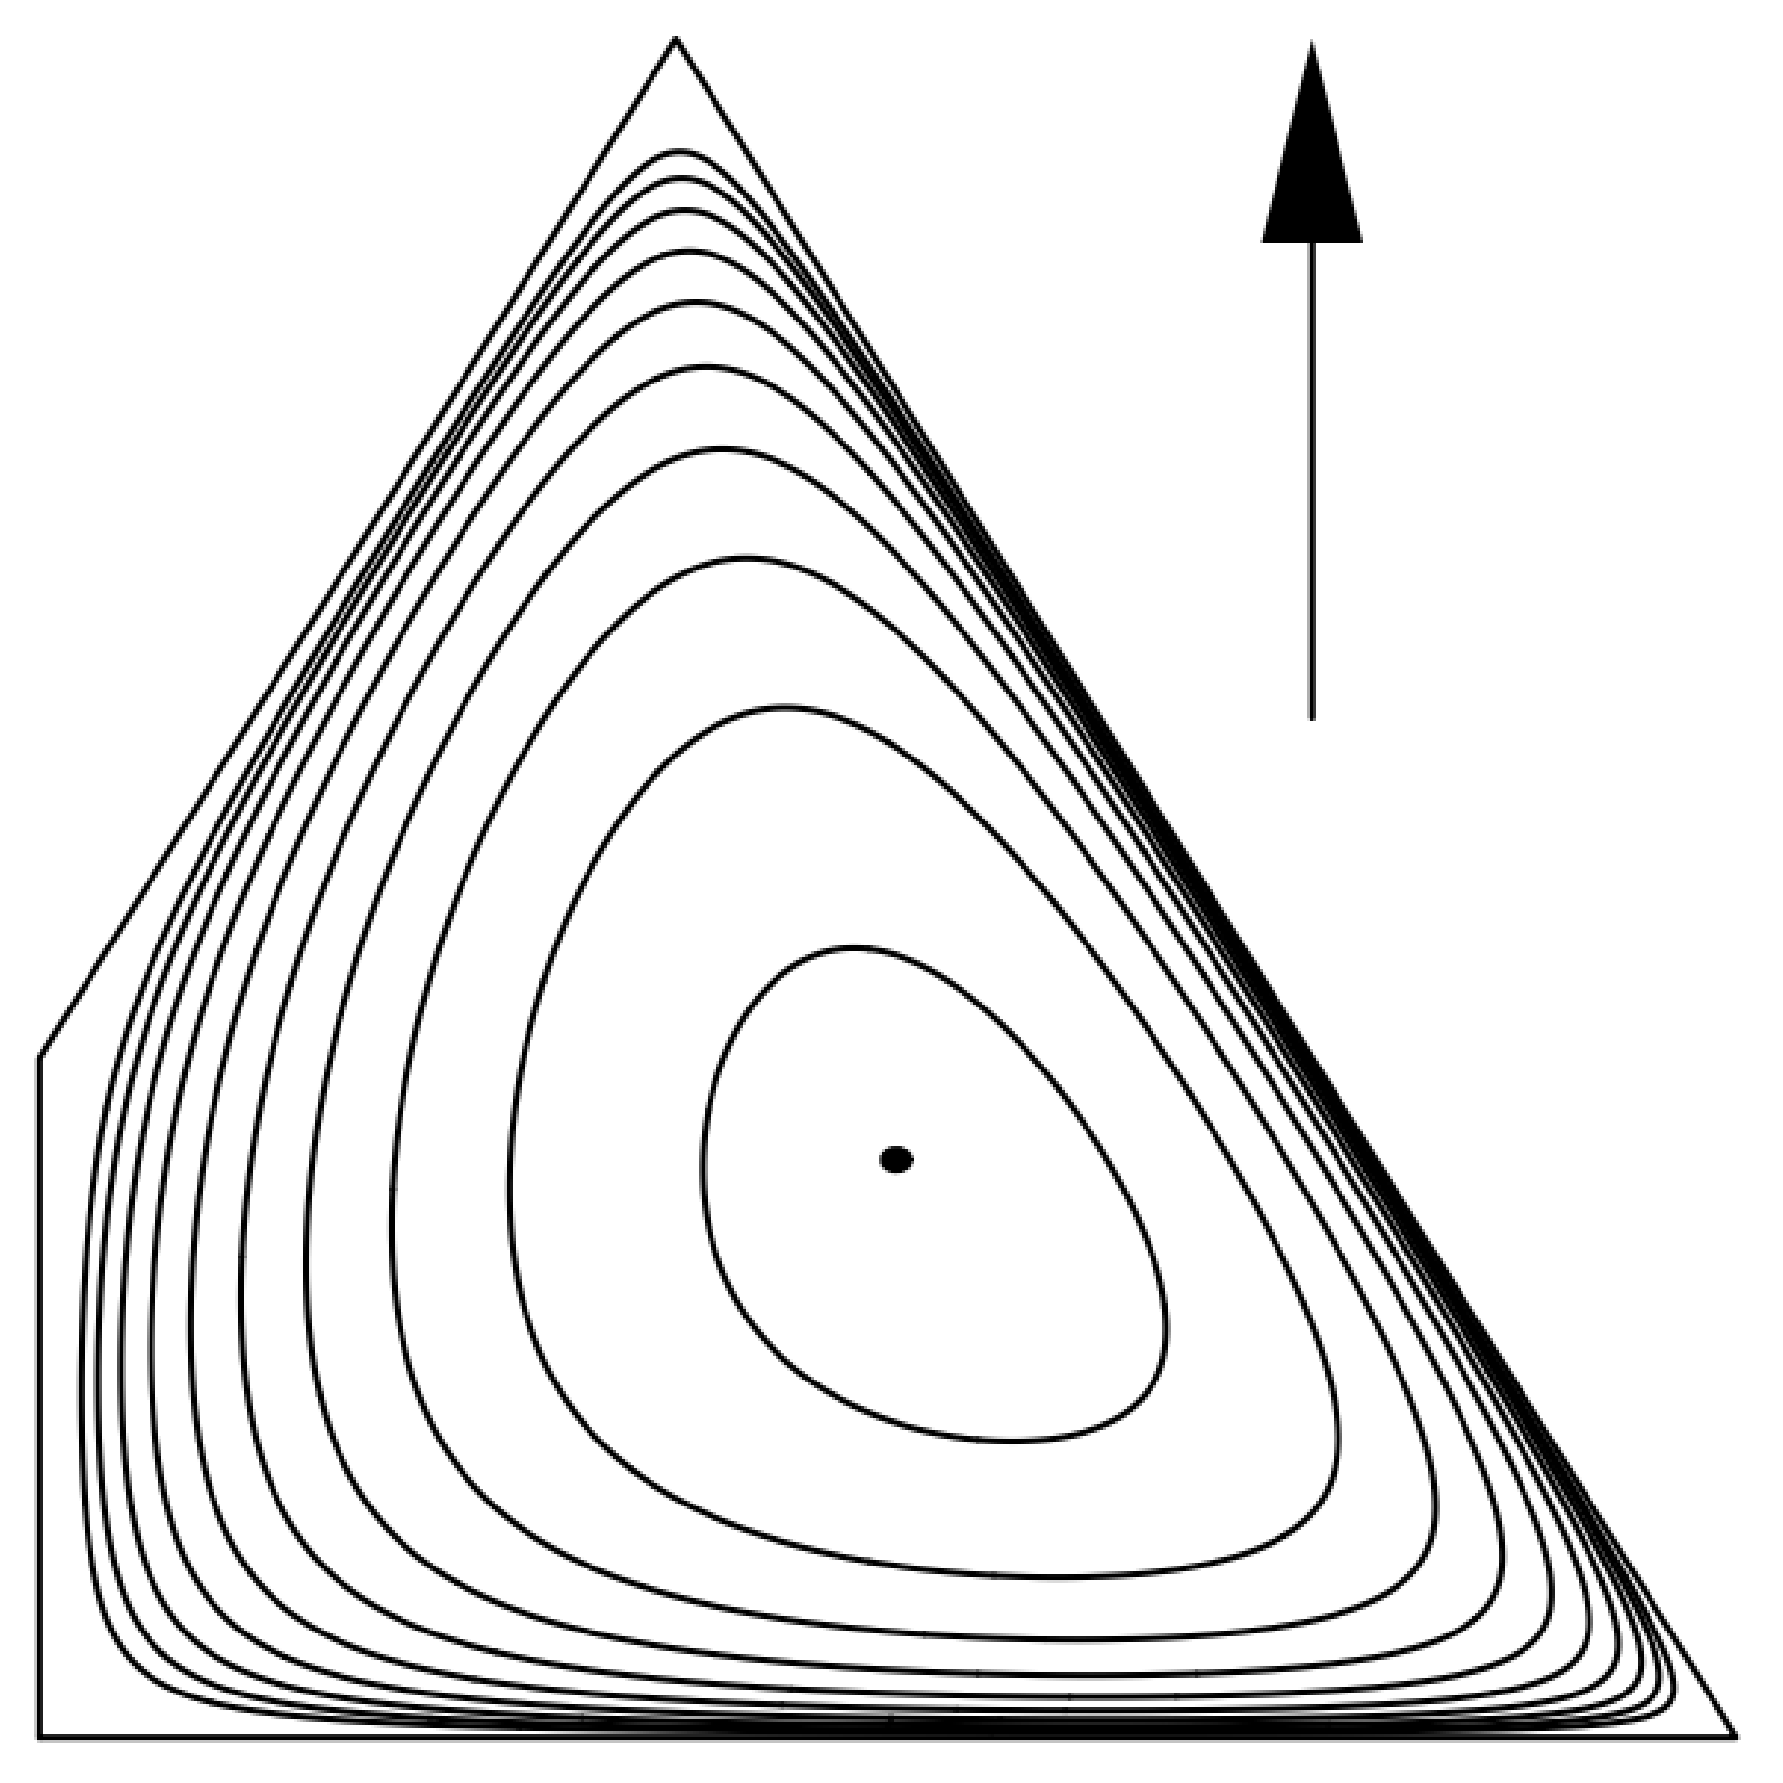
\includegraphics[width=0.25\textwidth]{img-14-1}
\caption*{Der Graph der Funktion $f_\mu(x)$ f�r den Fall $\mu = 100$.}
\end{figure}

\begin{figure}[H]
\centering
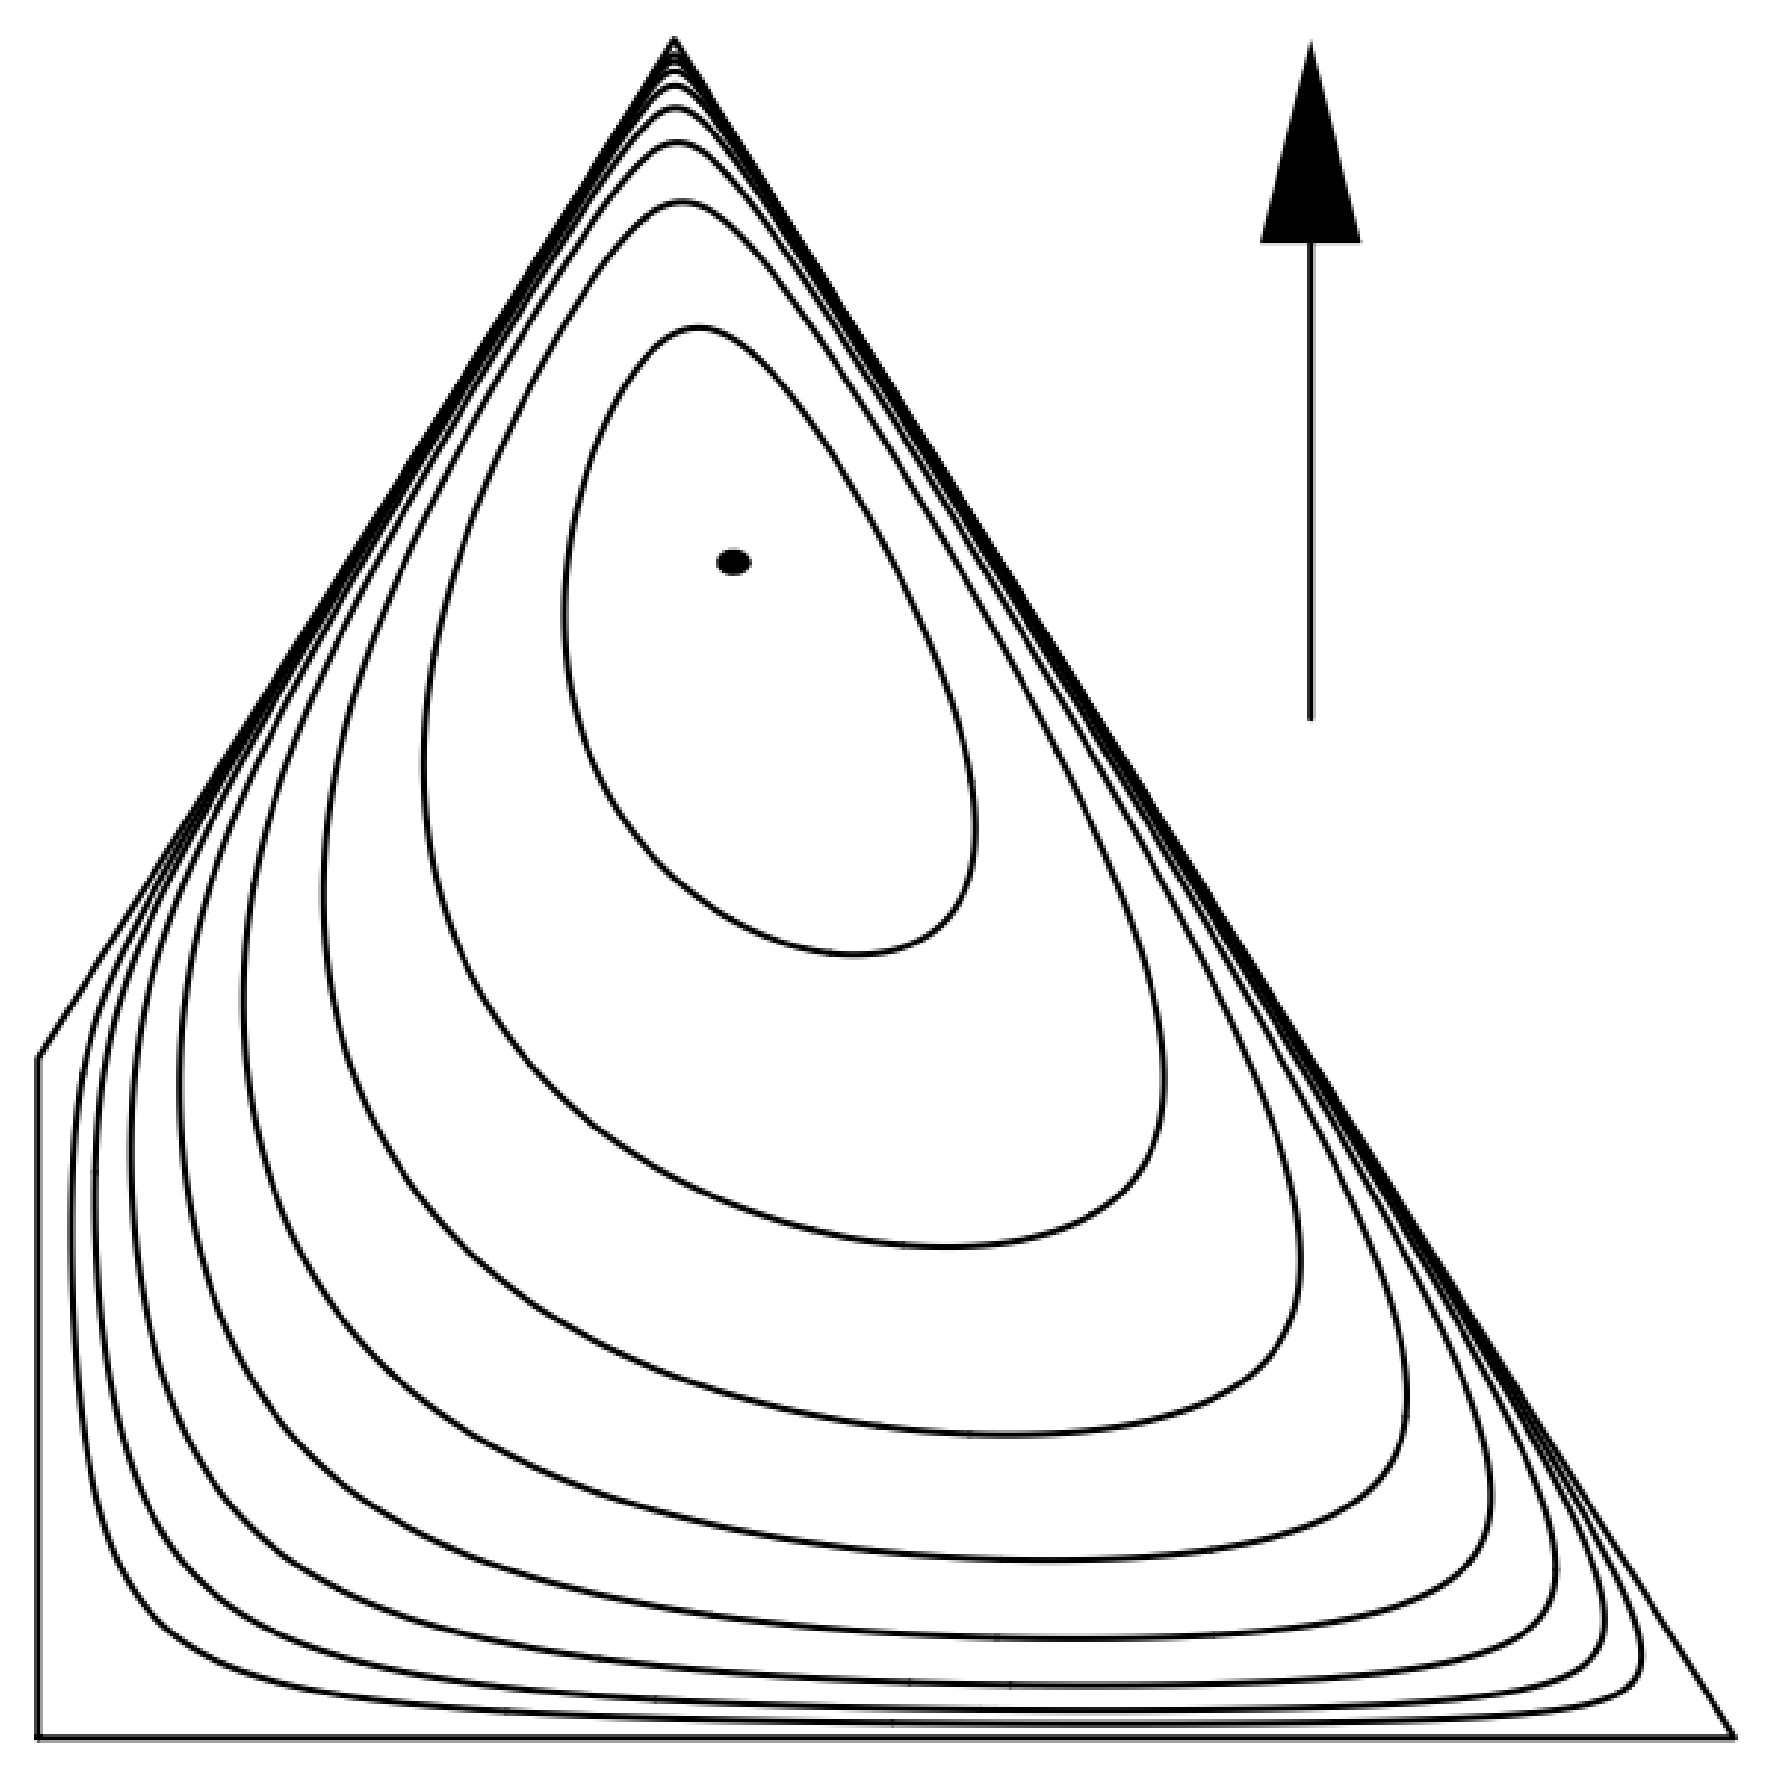
\includegraphics[width=0.25\textwidth]{img-14-2}
\caption*{Der Graph der Funktion $f_\mu(x)$ f�r den Fall $\mu = 0.5$.}
\end{figure}

\begin{figure}[H]
\centering
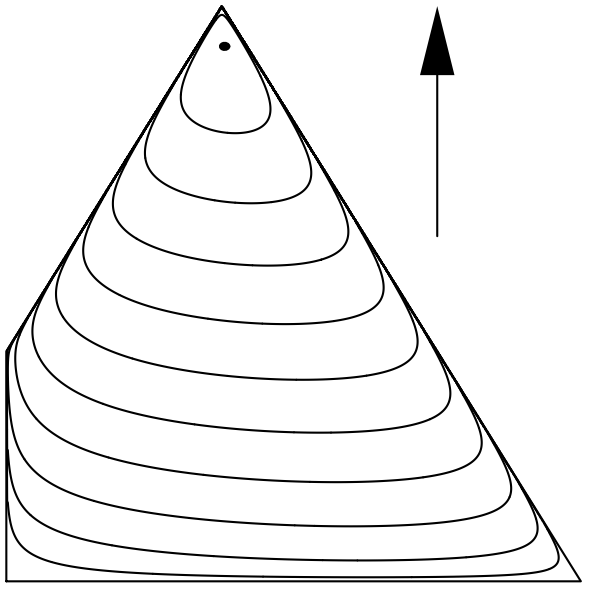
\includegraphics[width=0.25\textwidth]{img-14-3}
\caption*{Der Graph der Funktion $f_\mu(x)$ f�r den Fall $\mu = 0.1$.}
\end{figure}

\begin{Definition}[Definition der H�henlinien]
\index{H�henlinie}
Ist $f: \R^2 \rightarrow \R$ eine Funktion und $\alpha \in \R$, so definiert man die \textit{H�henlinie von $f$ zum Wert $\alpha$} als die Menge der Punkte $(x_1,x_2) \in \R^2$, f�r die $f(x_1,x_2)=\alpha$ gilt. 
\end{Definition}

Anders gesagt: Unter einer H�henlinie versteht man die Menge aller Punkte $(x_1,x_2)$, f�r die die Funktion $f$ einen vorgegebenen Wert (\enquote{H�he}) annimmt\footnote{H�henlinien werden nat�rlich analog definiert, wenn die betrachtete Funktion nur auf einer Teilmenge $D$ von $\R^2$ existiert.}.



\subsection{Der Begriff des zentralen Pfades}

Wir betrachten die im vorangegangenen Abschnitt definierten Maximalpunkte $x^*(\mu)$ und f�hren den Begriff des \enquote{zentralen Pfads} ein: Unter dem \textit{zentralen Pfad}\index{zentraler Pfad}\index{Pfad!zentraler} versteht man die Menge
\[
\Bigl\{ x^*(\mu) : \mu > 0 \Bigr\}.
\]

Der zentrale Pfad ist also die Menge aller Maximalpunkte $x^*(\mu)$ f�r $\mu > 0$. Es sei betont, dass der zentrale Pfad nicht nur von $P$ und der Zielfunktion $c$ abh�ngt, sondern auch von der Darstellung von $P$, d.h. vom Ungleichungssystem $Ax \leq b$, durch das $P$ gegeben ist: Dass dies so ist, erkennt man anhand von (\ref{eq:14:32}). 

Wir sind nun in der Lage, die \textit{Grundidee von Zentralen-Pfad-Methoden} zu formulieren.

\begin{Definition}[Grundidee von Zentralen-Pfad-Methoden]
Man startet mit einem $x^*(\mu)$ f�r ein geeignetes gro�es $\mu$ und folgt dann dem zentralen Pfad, indem man $\mu$ fortlaufend verkleinert.
\end{Definition}

Folgt man dieser Grundidee, so hat man -- wie wir zuvor gesehen haben -- in jedem Schritt ein Hilfsproblem mit einer nichtlinearen Zielfunktion $f_\mu(x)$ zu l�sen. Dadurch erh�lt man fortlaufend verbesserte N�herungswerte f�r die angestrebte L�sung des Problems
\begin{equation}
\label{eq:14:34}
\begin{alignedat}{3}
& \text{maximiere } & c^Tx & & \\
& \rlap{unter den Nebenbedingungen} & & & \\
&& Ax &\leq &\ b.
\end{alignedat}
\end{equation}

Zum Schluss geht es dann darum, wie man aus den gewonnenen N�herungsl�sungen eine exakte L�sung von (\ref{eq:14:34}) gewinnt.

\textit{Es g�be noch viele weitere Details zu besprechen}. Da es uns nur darum ging, die Grundideen darzulegen, brechen wir an dieser Stelle ab und verweisen auf das Buch von Matou\v{s}ek und G�rtner sowie auf die dort genannte Literatur.



%------------------------------------------------------------------------------%
% Skript zu:                                                                   %
% "Mathematik II f�r Studierende der Informatik"                               %
% ======================================================================       %
%                                                                              %
% Kapitel 15:                                                                  %
% "Literatur"                                                                  %
%                                                                              %
% in LaTeX gesetzt von:                                                        %
% Steven K�hler                                                                %
%                                                                              %
% Version:                                                                     %
% 2017-01-31                                                                   %
%------------------------------------------------------------------------------%

\chapter{Literatur}\label{chapter:literatur}

\begin{itemize}

\item D. Bertsimas, J. N. Tsitsiklis:

\textit{Introduction to Linear Optimization}. Athena Scientific. Belmont, Massachusetts. 1997.



\item A. Beutelspacher, M.-A. Zschiegner:

\textit{Diskrete Mathematik f�r Einsteiger}. Vieweg-Verlag. 2014. 5. Auflage.



\item V. Chv�tal:

\textit{Linear Programming}. W. H. Freeman and Company. New York. 2002. 16. Auflage.



\item Th. Cormen, Ch. Leiserson, R. Rivest, C. Stein:

\textit{Algorithmen -- Eine Einf�hrung}. Oldenbourg-Verlag. 2010. 3. Auflage. 



\item S. Dasgupta, C. Papadimitriou, U. Vazirani:

\textit{Algorithms}. McGraw Hill. 2008.



\item R. Diestel:

\textit{Graph Theory}. Springer. 2016. 5. Auflage.



\item M. Gr�tschel, L. Lov�sz, A. Schrijver: 

\textit{Geometric Algorithms and Combinational Optimization}. Springer. 1993. 3. Auflage.


\item D. Jungnickel:

\textit{Graphs, Networks and Algorithms}. Springer-Verlag. Berlin, Heidelberg, New York. 2012. 4. Auflage.



\item J. Kleinberg, �. Tardos:

\textit{Algorithm Design}. Pearson. Boston. 2006.



\item B. Korte, J. Vygen:

\textit{Combinatorial Optimization. Theory and Algorithms}. Springer. 2012. 5. Auflage.



\item N. Lauritzen: 

\textit{Undergraduate Convexity}. World Scientific. 2013.



\item L. Lov�sz, M. D. Plummer:

\textit{Matching Theory}. North-Holland. 1986.


\item D. Luenberger, Yinyu Ye:

\textit{Linear and Nonlinear Programming}. Springer. 2008. 3. Auflage.



\item J. Matou\v{s}ek, B. G�rtner:

\textit{Understanding and Using Linear Programming}. Springer-Verlag. Berlin, Heidelberg, New York. 2007.



\item K. Neumann, M. Morlock:

\textit{Operations Research}. Hanser-Verlag. 2004. 2. Auflage.



\item A. Schrijver:

\textit{Combinatorial Optimization. Polyhedra and Efficiency. Volume A: Paths, Flows, Matchings}. Springer. 2003.


\pagebreak

\item A. Schrijver:

\textit{Theory of Linear and Integer Programming}. Wiley. 1998.



\item A. Steger:

\textit{Diskrete Strukturen}. Band 1. Springer-Verlag. 2007.
\end{itemize}

\bigskip
Weitere n�tzliche Hinweise auf Literatur zur Linearen Optimierung sowie auf Software findet man in

\begin{itemize}
\item M. Gr�tschel:

\textit{Lineare Optimierung}. Skriptum zur Vorlesung im WS 2003/04. Technische Universit�t Berlin.
\end{itemize}


Zu guter Letzt sei der Klassiker auf dem Gebiet der Linearen Optimierung aufgef�hrt:

\begin{itemize}
\item G. B. Dantzig:

\textit{Linear Programming and Extensions}. Princeton University Press. 1963.
\end{itemize}


\printindex

\end{document}
